%-------------------------------------------------------------------------------
% This file provides a skeleton ATLAS document.
%-------------------------------------------------------------------------------
% Specify where ATLAS LaTeX style files can be found.
\newcommand*{\ATLASLATEXPATH}{latex/}
% Use this variant if the files are in a central location, e.g. $HOME/texmf.
% \newcommand*{\ATLASLATEXPATH}{}
%-------------------------------------------------------------------------------
\documentclass[UKenglish,texlive=2013]{\ATLASLATEXPATH atlasdoc}
% The following command is needed by arXiv to ensure use of pdflatex.
% It should be included in the first 5 lines of the preamble.
% \pdfoutput=1
% The language of the document must be set: usually UKenglish or USenglish.
% british and american also work!
% Commonly used options:
%  texlive=YYYY          Specify TeX Live version (2013 is default).
%  atlasstyle=true|false Use ATLAS style for document (default).
%  coverpage             Create ATLAS draft cover page for collaboration circulation.
%                        See atlas-draft-cover.tex for a list of variables that should be defined.
%  cernpreprint          Create front page for a CERN preprint.
%                        See atlas-preprint-cover.tex for a list of variables that should be defined.
%  PAPER                 The document is an ATLAS paper (draft).
%  CONF                  The document is a CONF note (draft).
%  PUB                   The document is a PUB note (draft).
%txfonts=true|false    Use txfonts rather than the default newtx - needed for arXiv submission.
%  paper=a4|letter       Set paper size to A4 (default) or letter.

%-------------------------------------------------------------------------------
% Extra packages:
\usepackage[subcaption,subfigure]{\ATLASLATEXPATH atlaspackage}
\usepackage{multirow}
% Commonly used options:
%  biblatex=true|false   Use biblatex (default) or bibtex for the bibliography.
%  backend=biber         Use the biber backend rather than bibtex.
%  subfigure|subfig|subcaption  to use one of these packages for figures in figures.
%  minimal               Minimal set of packages.
%  default               Standard set of packages.
%  full                  Full set of packages.
%-------------------------------------------------------------------------------
% Style file with biblatex options for ATLAS documents.
\usepackage{\ATLASLATEXPATH atlasbiblatex}

% Package for creating list of authors and contributors to the analysis.
\usepackage{\ATLASLATEXPATH atlascontribute}

\usepackage{rotating}


% Useful macros
\usepackage{\ATLASLATEXPATH atlasphysics}
% See doc/atlas-physics.pdf for a list of the defined symbols.
% Default options are:
%   true:  journal, misc, particle, unit, xref
%   false: BSM, hion, math, process, other, texmf
% See the package for details on the options.

% Files with references for use with biblatex.
% Note that biber gives an error if it finds empty bib files.
\addbibresource{ss3l2015.bib}
\addbibresource{bibtex/bib/ATLAS.bib}
\addbibresource{bibtex/bib/PubNotes.bib}
\addbibresource{bibtex/bib/ConfNotes.bib}

% Paths for figures - do not forget the / at the end of the directory name.
\graphicspath{{logos/}{FIGURES/}}

% Add you own definitions here (file ss3l2015-defs.sty).
\usepackage{ss3l2015-defs}


%-------------------------------------------------------------------------------
% Generic document information
%-------------------------------------------------------------------------------

% Title, abstract and document 
%-------------------------------------------------------------------------------
% This file contains the title, author and abstract.
% It also contains all relevant document numbers used by the different cover pages.
%-------------------------------------------------------------------------------

% Title
\AtlasTitle{Search for strongly produced superpartners in final states with same-sign leptons or three leptons and jets in $pp$ collisions at $\sqrt{s}=13$~TeV (Supporting note)}

% Author - this does not work with revtex (add it after \begin{document})
%\author{The ATLAS Collaboration}

% Authors and list of contributors to the analysis
% \AtlasAuthorContributor also adds the name to the author list
% Include package latex/atlascontribute to use this
% Use authblk package if there are multiple authors, which is included by latex/atlascontribute
\usepackage{authblk}
\renewcommand\Authands{, } % avoid ``. and'' for last author
\renewcommand\Affilfont{\itshape\small} % affiliation formatting
%\AtlasAuthorContributor{The SS/3L analysis team}{a}{Everything}
%\affil[a]{all}

\AtlasAuthorContributor{B.~Abbott}{1}{Supervision of students}
\AtlasAuthorContributor{J.-F.~Arguin}{2}{Charge flip studies, supervision of students}
\AtlasAuthorContributor{S.~Berlendis}{3}{Generation of background MC}
\AtlasAuthorContributor{F.~Cardillo}{4}{Event selection (lepton pairing), trigger strategy, MC15 signal region optimization, tree production with experimental systematic uncertainties, HistFitter statistical interpretation, production of exclusion plots}
\AtlasAuthorContributor{G.~Carrillo-Montoya}{5}{Event selection ($b$-tagging, overlap removal), DPS cross-checks}
\AtlasAuthorContributor{A.~Di~Simone}{4}{HistFitter statistical interpretation, production of exclusion plots, supervision of students}

\AtlasAuthorContributor{O.~Ducu}{6,7}{Event selection (electron acceptance), DC14 signal regions optimization, fake-lepton background estimation and composition studies, validation regions definitions, data/MC comparisons}

\AtlasAuthorContributor{D. Gerbaudo}{8}{Generation of background MC, theory uncertainties}

\AtlasAuthorContributor{F.~Hubaut}{7}{Supervision of students}

\AtlasAuthorContributor{G.~Herten}{4}{Supervision of students}

\AtlasAuthorContributor{S.~Kahn}{7}{Real lepton efficiency studies, study of pMSSSM models}

\AtlasAuthorContributor{A.~Lleres}{3}{Supervision of students}
\AtlasAuthorContributor{J.~Maurer}{6}{Analysis coordination, editor of supporting note, CONF note and paper; signal sample generation, background estimation cross-checks}
\AtlasAuthorContributor{E.~Monnier}{7}{Supervision of students}
\AtlasAuthorContributor{T.~Nguyen}{2}{Charge flip background estimation}

\AtlasAuthorContributor{A.~Paramonov}{9}{Rare processes evaluation, supervision of students}
\AtlasAuthorContributor{J.~Poveda}{5}{Analysis coordination, editor of supporting note, CONF note and paper; ntuple production, event selection (lepton isolation), data/MC comparisons, MC15 signal region optimization}
\AtlasAuthorContributor{P.~Pralavorio}{7}{Supervision of students}

\AtlasAuthorContributor{H.~Ren}{10, 7}{Fake lepton background estimation}
\AtlasAuthorContributor{O.~Rifki}{1}{MC template method, data/MC comparisons, background estimation cross-checks}
\AtlasAuthorContributor{Y.-T.~Shen}{1}{25/50ns MC comparisons, isolation SF studies}
\AtlasAuthorContributor{P.~Skubic}{1}{Supervision of students}

\AtlasAuthorContributor{A.~Taffard}{8}{Supervision of students}

\AtlasAuthorContributor{P.~Tornamb\'{e}}{4}{Event selection (lepton pairing), MC15 signal region optimization, tree production with experimental systematic uncertainties, HistFitter statistical interpretation, production of exclusion plots}

\AtlasAuthorContributor{H.~Tr\'{e}panier}{2}{Charge flip background}
\AtlasAuthorContributor{X.~Zhuang}{10}{Supervision of students}


%\AtlasAuthorContributor{Second AtlasAuthorContributor}{b}{Author's contribution.}
% \AtlasAuthorContributor{Third AtlasAuthorContributor}{a}{Author's contribution.}
% \AtlasContributor{Fourth AtlasContributor}{Contribution to the analysis.}
%\author[a]{The SS/3L analysis team}
% \author[a]{Second Author}
% \author[b]{Third Author}
%\affil[a]{all}
\affil[1]{University of Oklahoma}
\affil[2]{Universit\'e de Montr\'eal}
\affil[3]{Laboratoire de Physique Subatomique et de Cosmologie de Grenoble (LPSC)}
\affil[4]{Albert-Ludwigs-Universit\"at Freiburg}
\affil[5]{European Laboratory for Particle Physics, CERN}
\affil[6]{Horia Hulubei National Institute for R\&D in Physics and Nuclear Engineering (IFIN-HH) Bucharest}
\affil[7]{Centre de Physique des Particules de Marseille (CPPM)}
\affil[8]{University of California, Irvine}
\affil[9]{Argonne National Laboratory}

\affil[10]{Institute of High Energy Physics, Chinese Academy of
Sciences, Beijing}


% If a special author list should be indicated via a link use the following code:
% Include the two lines below if you do not use atlasstyle:
% \usepackage[marginal,hang]{footmisc}
% \setlength{\footnotemargin}{0.5em}
% Use the following lines in all cases:
% \usepackage{authblk}
% \author{The ATLAS Collaboration%
% \thanks{The full author list can be found at:\newline
%   \url{https://atlas.web.cern.ch/Atlas/PUBNOTES/ATL-PHYS-PUB-2014-007/authorlist.pdf}}
% }

% Date: if not given, uses current date
\date{\today}

% Draft version:
% Should be 1.0 for the first circulation, and 2.0 for the second circulation.
% If given, adds draft version on front page, a 'DRAFT' box on top of each other page, 
% and line numbers.
% Comment or remove in final version.
\AtlasVersion{2.1}

% ATLAS reference code, to help ATLAS members to locate the paper
\AtlasRefCode{SUSY-2015-09}

% ATLAS note number. Can be an COM, INT, PUB or CONF note
% \AtlasNote{ATLAS-CONF-2014-XXX}
% \AtlasNote{ATL-PHYS-PUB-2014-XXX}
% \AtlasNote{ATL-COM-PHYS-2014-XXX}

% CERN preprint number
% \PreprintIdNumber{CERN-PH-2014-XX}

% ATLAS date - arXiv submission; to be filled in by the Physics Office
% \AtlasDate{\today}

% arXiv identifier
% \arXivId{14XX.YYYY}

% HepData record
% \HepDataRecord{ZZZZZZZZ}

% Submission journal and final reference
% \AtlasJournal{Phys.\ Lett.\ B.}
% \AtlasJournalRef{\PLB 789 (2014) 123}
% \AtlasDOI{}

% Abstract - % directly after { is important for correct indentation
\AtlasAbstract{%
% This note contains the documentation of the studies performed with MC15 Monte Carlo samples and early data in preparation for the Run-2 search for strongly produced supersymmetric particles using signatures involving multiple energetic jets and either two isolated leptons ($e$ or $\mu$) with the same electric charge, or at least three isolated leptons.
%The analysis also utilises jets originating from $b$-quarks, missing transverse momentum and other observables to extend its sensitivity.
A search for strongly produced supersymmetric particles is conducted using signatures involving multiple energetic jets and either two isolated leptons ($e$ or $\mu$) with the same electric charge, or at least three isolated leptons. The search also utilises jets originating from $b$-quarks, missing transverse momentum and other observables to extend its sensitivity. The analysis uses a data sample corresponding to a total integrated luminosity of XX fb$^{-1}$ of $\sqrt{s}= 13$~TeV proton-proton collisions recorded with the ATLAS detector at the Large Hadron Collider in 2015. (Add results).

}

%-------------------------------------------------------------------------------
% The following information is needed for the cover page. The commands are only defined
% if you use the coverpage option in atlasdoc or use the atlascover package
%-------------------------------------------------------------------------------

% List of supporting notes  (leave as null \AtlasCoverSupportingNote{} if you want to skip this option)
% \AtlasCoverSupportingNote{Short title note 1}{https://cds.cern.ch/record/XXXXXXX}
% \AtlasCoverSupportingNote{Short title note 2}{https://cds.cern.ch/record/YYYYYYY}
%
% OR (the 2nd option is deprecated, especially for CONF and PUB notes)
%
% Supporting material TWiki page  (leave as null \AtlasCoverTwikiURL{} if you want to skip this option)
% \AtlasCoverTwikiURL{https://twiki.cern.ch/twiki/bin/view/Atlas/WebHome}

% Comment deadline
% \AtlasCoverCommentsDeadline{DD Month 2014}

% Analysis team members - contact editors should no longer be specified
% as there is a generic email list name for the editors
% \AtlasCoverAnalysisTeam{Peter Analyser, Susan Editor1, Jenny Editor2, Alphonse Physicien}

% Editorial Board Members - indicate the Chair by a (chair) after his/her name
% Give either all members at once (then they appear on one line), or separately
% \AtlasCoverEdBoardMember{EdBoard~Chair~(chair), EB~Member~1, EB~Member~2, EB~Member~3}
% \AtlasCoverEdBoardMember{EdBoard~Chair~(chair)}
% \AtlasCoverEdBoardMember{EB~Member~1}
% \AtlasCoverEdBoardMember{EB~Member~2}
% \AtlasCoverEdBoardMember{EB~Member~3}

% A PUB note has readers and not an EdBoard -- give their names here (one line or several entries)
% \AtlasCoverReaderMember{Reader~1, Reader~2}
% \AtlasCoverReaderMember{Reader~1}
% \AtlasCoverEdBoardMember{Reader~2}

% Editors egroup
% \AtlasCoverEgroupEditors{atlas-GROUP-2014-XX-editors@cern.ch}

% EdBoard egroup
% \AtlasCoverEgroupEdBoard{atlas-GROUP-2014-XX-editorial-board@cern.ch}


% Author and title for the PDF file
\hypersetup{pdftitle={Supporting note draft},pdfauthor={SUSY SS/3L team}}


%-------------------------------------------------------------------------------
% Content
%-------------------------------------------------------------------------------
\begin{document}

\maketitle

\tableofcontents

% List of contributors - print here or after the Bibliography.
\clearpage
\PrintAtlasContribute{0.30}
\clearpage

%-------------------------------------------------------------------------------
%\setcounter{section}{-1}
%\section{Notes to the reader}
%\label{sec:notesReader}
%Please note that some parts of the note are still work in progress and will be finalized soon.
The Sections where updates are foreseen in the near future will be clearly stated in the text. 
Also note that the results in the note will be updated as more data is available.


\paragraph{Updates and pending items in version 1.1 (ATLAS draft 1 circulation):}
\begin{itemize}
\item Updates included with respect to previous version:
\begin{itemize}
\item Results updated with 3.3~fb$^{-1}$ (EOYE recommendation not included yet)
\item Trigger matching and SF for dilepton trigger
\item More HistFitter details
\end{itemize}

\item Pending items: 
\begin{itemize}
\item EOYE recommendations
\item Trigger SF for muons
\end{itemize}

\end{itemize}

\paragraph{Updates and pending items in version 1.0 (SUSY WG circulation):}
\begin{itemize}
\item Updates included with respect to previous version:
\begin{itemize}
\item Unblinded results for 2.7~fb$^{-1}$, section~\ref{sec:fit}
\item Detailed investigations of the VRs, appendix~\ref{appendix:ttV}
\item Final parametrization of syst uncertainties for real lepton efficiencies (section~\ref{sec:RealRate_DD}, appendix~\ref{App:RealEfficiency})
\item distributions of number of vertices in data/MC after pile-up reweighting, appendix~\ref{appendix:pileup_checks}
\end{itemize}

\item Pending items: 
\begin{itemize}
\item Quantitative description of the systematic uncertainties (experimental and theory-related)
\item Description of the HistFitter setup, and signal model exclusion plots
\item Check for duplicates on MC
\item Add stability tests
\item Trigger matching and SF
\end{itemize}

\end{itemize}

%\paragraph{Updates and pending items in version 0.3:}
%\begin{itemize}
%\item Updates included with respect to previous version:
%\begin{itemize}
%\item Update of section~\ref{subsec:signal_models} (signal models), mostly to add a description of the scenario with gluino two-step decays via sleptons
%\item Added DSIDs info for signal models in section~\ref{sec:SigSamples}
%\item Final definitions and results in the validation regions
%\item New ABCD method cross-check of the fake lepton background estimate in the signal region with 3 $b$-jets, described in section~\ref{sec:bkg_abcd_method}
%\item Unblinded results for 1.7~fb$^{-1}$, section~\ref{sec:fit}
%\item Edited sections~\ref{sec:bkg_fakes} and~\ref{sec:bkg_matrix_method} : description of the fake rate measurement (with latest results) and motivaiton for systematics
%\item Added details on evaluation of contributions from double parton scattering (section~\ref{sec:bkg_neglected}).
%\item Update of real lepton efficiency measurements, evaluation of the systematics (section~\ref{sec:bkg_matrix_method})
%\item Update of charge flip rate measurements, and related systematics, in section~\ref{sec:bkg_chflips}
%\end{itemize}
%
%\item Pending items: 
%\begin{itemize}
%\item Quantitative description of the systematic uncertainties (experimental and theory-related)
%\item Presentation of the observations in the signal regions
%\item Description of the HistFitter setup, and signal model exclusion plots
%\end{itemize}
%
%\end{itemize}

%\paragraph{Updates and pending items in version 0.2:}
%\begin{itemize}
%\item Updates included with respect to previous version:
%\begin{itemize}
%\item Data results extended to 1~fb$^{-1}$ of data
%\item Signal region optimization finalized
%\item Parametrization of real and fake lepton efficiencies
%\item Electron charge flip rates for baseline electrons added
%\item Extend the evaluation of fake efficiencies to $10<\pt<15$~GeV
%\end{itemize}
%\item Pending items: 
%\begin{itemize}
%\item Figures in Section 8.1 are missing due to a SVN conflict, will be added asap 
%\item Systematics for real and fake lepton efficiencies
%\item Evaluation of theory systematics, quantitative presentation of the experimental systematics
%\item Evaluation of sensitivity with HistFitter
%\item Extend the evaluation of real efficiencies to $10<\pt<15$~GeV
%\item Alternative estimation for background with fake $b$-jets
%\end{itemize}
%\end{itemize}

%\paragraph{Pending items in version 0.1:}
%
%\begin{itemize}
%\item Finalize signal region optimization and validation region definition
%\item Parametrization and systematics for real and fake lepton efficiencies
%\item Electron charge flip rates for baseline electrons
%\item Alternative estimation for background with fake $b$-jets
%\item Evaluation of theory systematics, quantitative presentation of the experimental systematics
%\item Evaluation of sensitivity with HistFitter
%\item Extend the evaluation of real and fake efficiencies to $10<\pt<15$~GeV
%\end{itemize}


%-------------------------------------------------------------------------------
\section{Introduction}
\label{sec:intro}
%-------------------------------------------------------------------------------
% why study elementary particles
% the sucess of the standard model
% the need for bsm: supersymmetry
% the tool to do it: LHC and ATLAS 
% the challenge

% How did we get here?

Of what is the universe made? A question that has intrigued the human curiosity since the dawn of time. 
Today, we are confident that we do not know the answer to this question but a lot of progress has been made
The overeaching aim was to reduce the diversity of the physicsal phenomena to a compact set of constituents
and a unified set of principles.
% Unification and symmetry
%Yet, attempts to answer it has gone through many iterations in order to find a compact set of principles
%that offers a syntheis of the phenomena we observe in the world around us. 
%would describe the world we observe.
%where it was deemed solved at times 
%and unreachable at others. 
Over two thousands years ago, the ancient Greeks  postulated that all is made of Earth, Air, Fire and Water. 
The idea behind this picture is to give a description of the world we observe based on a compact set of principles 
Obvisoulsy, the ancients got it wrong.
Fastfoward to the end of the 19th century, Mendeleev and others made the astonishing remark that by organizing the 
relative atomic masses of chemical elements in an ascending order, elements with similar chemical properties followed a pattern.
The periodic table of elements was born. 
The predictive power of the periodic table led to the anticipation of new elements and their properties that were later discovered.
However, the table lacked compactness and necessitated a more fundamental underlying structure that could 
connect the different elements. At the turn of the century, several important discoveries established 
the existence of the atom and its constituents. The mass of the atom lies in its nucleus with electrons bound to it via the 
electromagnetic force. The nucleus itself is formed from 
protons and neutrons that are ``glued'' togehter by the strong nuclear force (or strong force).
These elements formed the underlying substructure that explained qualitatively the systematic organization of the periodic table.
Moreover, quantum ideas were applied to the atom offering a quantitative description of the origin of structure in atoms and molecules, 
including the chemical elements and their properties.
The decades that followed refined our understanding of the composition of matter through a series of experimental results.
By studying the collisions of protons and neutrons in the 50's and 60's, we came to uncover a plethora of new particles from the same 
family as the proton and neutron which interacted via the strong force, called \textit{hadrons}.
These particles could not be all elementary
\footnote{Elementary particles refer to  particles that cannot be decomposed into further constituents.}
, a classic replay of the argument that atoms were composite based on Mendeleev's table.
A new layer of structure was unfolded to reveal the existence of \textit{quarks}, elementary 
particles that interact via the strong force and make up all hadrons. 
Another puzzle of the 20th century was the continuous energy spectra in the radioactive $\beta$ decay of nuclei which pointed to the 
existence of neutrinos to remedy the energy conservation law in the decay. This process proceeds via the weak nuclear force 
repsonsible for the radioactivity and nuclear fusion, the process that powers the stars.
It turns out that electrons and neutrinos had other relatives referred to as \textit{leptons}.
Similarly, several other quarks were discovered.%, with the latest top quark discovered in 1995. 
The quarks and leptons are collectively referred as fermions and
share a half integer spin, an intrinsic property of elementary particles.
The strong, weak, and electromagnetic interactions are mediated by 
gluons, $W$ and $Z$ bosons, and photons. These are 
elementary particles with an integer spin, 
collectively called bosons. Apart from gravity, all aspects of daily life can 
be described in terms of these interactions.
%The gravitational force is so weak that it only acts at the macroscopic scale.
The lastest discovery happened in 2012 of a new boson, the Higgs boson, 
that allows the quarks and leptons and the $W$ and $Z$ bosons to 
acquire mass.

%A success story
The physics of elementary particles became the most ambitious and organized attempt to answer the question of what the universe is 
made out of. 
Through a mixture of both theorertical insight and experimental input, we now 
know that everything we see in our daily life is formed from quarks and leptons
that interact via the strong, weak, and electromagnetic forces. 
The forms of these forces are determined from basic princples of 
symmetry and invariance.
As a result, a theoretical framework was constructed to synthesize all these 
developments in a quantitative 
calculational tool that became known as the \textit{Standard Model of particle physics} (SM). 
The only inputs needed by the SM are the interaction strengths of the forces and quark and lepton masses to make 
very accurate predictions about the behavior of elementary particles.
For example, the magnetic moment of the electron calculated in the SM is found to agree with the experimental measurement to nine(?) decimal places.
Over the past 30 years, the SM has been vigorously tested across the strong, weak, and electromagnetic interactions. 
It came out triumphant every time. Yet, we know it is not the complete story. 

% the dark side
In 1933, an observation of the Coma Cluster by Zwicky suggested that the galaxies in the cluster were moving too fast to be explained 
by the luminous matter present. The same observation was repeated when looking at the rotation speeds of individual galaxies which 
suggested a dark component of mass, Dark Matter. 
Several independent measurements established that 
not only dark matter is not made out of baryons but it is more 
abundant. 
For example, anistropies in the cosmic microwave background, a radiation 
left over from the Big Bang, were consistent with 
quantum fluctuations from an inflationary epoch \cite{Hu:2001bc,2009AIPC}. 
These fluctuations encoded details about the density of matter 
in the form of 
cosmological parameters as they travelled through space and time to reach 
our experiments.
The astonishing conclusion was that the universe has nearly five times 
as much dark matter as ordinary matter \cite{Bertone:2004pz}.
The supernovae surveys gave direct evidence for an accelerating universe
 \cite{Perlmutter:1998np},
a view that was cemented by the measurement of cosmological parameters
\cite{Adam:2015rua,Ade:2015xua}
which led to the startling discovery that most of the energy density of 
the Universe is in the 
form of an unkown negative-pressure, called dark energy \cite{Scranton:2003in}.
There is an extensive program of experiments 
which will probe the dark energy.% and is beyond the scope of this work. 
%Instead, we turn to dark matter. 
Astrophysics and cosmology told us about 
the existence of dark matter and measured its density to a remarkable 
precision. Particle physics holds the hope to uncover what dark matter is.
In short, all experimental evidence are consistent with a universe 
constructed of 
\begin{itemize}
\item baryons (everyday matter): $\sim 5\%$ 
\item dark matter: $\sim 20\%$ 
\item dark energy: $\sim 75\%$ 
\item neutrinos, photons: a tiny fraction
\end{itemize}

Today, we are in front of many puzzles related to our view of the universe.
Everything we know of, including all particles present in the standard model, 
constitutes only 5\% of the energy budget of the universe. 
The universe is also predominatly composed of matter as opposed to 
anti-matter even though at the start of the universe, they were in equal 
amounts%, baryon assymetry
. The standard model describes the content of 
everyday matter 
and how it interacts but without telling us why it is that way.
Moreover, the standard model only describes these phenomena 
up to an energy scale of $\mathcal{O}\left(100\right)$ \GeV, weak scale.
Beyond this scale lies the realm of phenomena not described by the standard 
model that extend all the way to the Planck scale of 
$\mathcal{O}\left(10^{19}\right)$ \GeV, the limit where the known laws of 
physics apply. 
There is no mechanism to generate mass for 
neutrinos in the standard model. Last but not least, the standard model 
does not incorporate gravity, the fourth fundamental force.
The SM has many limitations since it is unable to account for observed 
features in the universe. 
Thus, there is a need for a theory beyond the standard model.

One of the most prominent extensions of the standard model, 
that addresses many of the shortcomings mentioned above, is a theory based on 
a new symmetry, called supersymmetry.
This symmetry is between the matter particles, fermions, and particles whose
exchange mediates the forces, bosons. Our current description of the world
treats fermions and bosons differently. Supersymmetry puts forward the idea
that fermions and bosons can be treated in a fully symmetric way. 
In other words,
if we exchange fermions and bosons in the equations of the theory, the 
equations will still look the same. An immediate consequence of the theory
is that every standard model particle will have a ``superpartner''.
As a result, we can design experiments to search for these 
supersymmetric particles. The work presented in this thesis is about the search for supersymmetric particles with a specific signature.
The many benefits of supersymmetry will be discussed but here it is worth 
mentioning two important features of the theory: it addresses the question 
of why there is a huge gap between the Planck scale and the weak scale, 
and it provides a dark matter candidate particle. 

Now that we understand what we are trying to do, it is time to address 
the question of how to do it.
For this endeavour, we require two key elements: accelerators and detectors.
The Large Hadron Collider (LHC) at CERN is the world's most energetic 
particle accelerator producing the highest intensity beam of protons 
travelling at 99.99993\% the speed of light. 

colliding beams of proton beams at a center of mass 
energy of 13 \TeV. When two protons collide, many new paerticles are 
created out of 


Many years of experience from Tevatron collider at Fermilab\cite{tevatron}, 
HERA at DESY\cite{hera}, and LEP\cite{lep} at CERN improved the understanding of the 
complex strong interaction dynamics 


% complex detectors


%-------------------------------------------------------------------------------
%\section{ATLAS detector}
%\label{sec:detector}
%-------------------------------------------------------------------------------

%The ATLAS detector~\cite{PERF-2007-01} ...
% % Footnote with ATLAS coordinate system
\newcommand{\AtlasCoordFootnote}{%
ATLAS uses a right-handed coordinate system with its origin at the nominal interaction point (IP)
in the centre of the detector and the $z$-axis along the beam pipe.
The $x$-axis points from the IP to the centre of the LHC ring,
and the $y$-axis points upwards.
Cylindrical coordinates $(r,\phi)$ are used in the transverse plane, 
$\phi$ being the azimuthal angle around the $z$-axis.
The pseudorapidity is defined in terms of the polar angle $\theta$ as $\eta = -\ln \tan(\theta/2)$.
Angular distance is measured in units of $\Delta R \equiv \sqrt{(\Delta\eta)^{2} + (\Delta\phi)^{2}}$.}

%-------------------------------------------------------------------------------
\subsection{ATLAS detector example from a Letter}
\label{sec:atlas1}
%-------------------------------------------------------------------------------

The ATLAS experiment~\cite{PERF-2007-01} at the LHC is a multi-purpose particle detector
with a forward-backward symmetric cylindrical geometry and a near $4\pi$ coverage in 
solid angle.\footnote{\AtlasCoordFootnote}
It consists of an inner tracking detector surrounded by a thin superconducting solenoid
providing a \SI{2}{\tesla} axial magnetic field, electromagnetic and hadron calorimeters, and a muon spectrometer.
The inner tracking detector covers the pseudorapidity range $|\eta| < 2.5$.
It consists of silicon pixel, silicon micro-strip, and transition radiation tracking detectors.
Lead/liquid-argon (LAr) sampling calorimeters provide electromagnetic (EM) energy measurements
with high granularity.
A hadron (iron/scintillator-tile) calorimeter covers the central pseudorapidity range ($|\eta| < 1.7$).
The end-cap and forward regions are instrumented with LAr calorimeters
for both EM and hadronic energy measurements up to $|\eta| = 4.9$.
The muon spectrometer surrounds the calorimeters and is based on
three large air-core toroid superconducting magnets with eight coils each.
Its bending power is in the range from \num{2.0} to \SI{7.5}{\tesla\metre}.
It includes a system of precision tracking chambers and fast detectors for triggering.
A three-level trigger system is used to select events.
The first-level trigger is implemented in hardware and uses a subset of the detector information
to reduce the accepted rate to at most \SI{75}{\kilo\hertz}.
This is followed by two software-based trigger levels that
together reduce the accepted event rate to \SI{400}{\hertz} on average
depending on the data-taking conditions during 2012.


%-------------------------------------------------------------------------------
\subsection{ATLAS detector example from a paper making use of the whole detector}
\label{sec:atlas2}
%-------------------------------------------------------------------------------

The ATLAS detector~\cite{PERF-2007-01} at the LHC covers nearly the entire solid angle around the collision point.
It consists of an inner tracking detector surrounded by a thin superconducting solenoid, electromagnetic and hadronic calorimeters,
and a muon spectrometer incorporating three large superconducting toroid magnets.
The inner-detector system (ID) is immersed in a \SI{2}{\tesla} axial magnetic field 
and provides charged particle tracking in the range $|\eta| < 2.5$.

The high-granularity silicon pixel detector covers the vertex region and typically provides three measurements per track, 
the first hit being normally in the innermost layer.
It is followed by the silicon microstrip tracker which usually provides four two-dimensional measurement points per track.
These silicon detectors are complemented by the transition radiation tracker,
which enables radially extended track reconstruction up to $|\eta| = 2.0$. 
The transition radiation tracker also provides electron identification information 
based on the fraction of hits (typically 30 in total) above a higher energy deposit threshold corresponding to transition radiation.

The calorimeter system covers the pseudorapidity range $|\eta| < 4.9$.
Within the region $|\eta|< 3.2$, electromagnetic calorimetry is provided by barrel and 
endcap high-granularity lead/liquid-argon (LAr) electromagnetic calorimeters,
with an additional thin LAr presampler covering $|\eta| < 1.8$,
to correct for energy loss in material upstream of the calorimeters.
Hadronic calorimetry is provided by the steel/scintillating-tile calorimeter,
segmented into three barrel structures within $|\eta| < 1.7$, and two copper/LAr hadronic endcap calorimeters.
The solid angle coverage is completed with forward copper/LAr and tungsten/LAr calorimeter modules
optimised for electromagnetic and hadronic measurements respectively.

The muon spectrometer (MS) comprises separate trigger and
high-precision tracking chambers measuring the deflection of muons in a magnetic field generated by superconducting air-core toroids.
The precision chamber system covers the region $|\eta| < 2.7$ with three layers of monitored drift tubes,
complemented by cathode strip chambers in the forward region, where the background is highest.
The muon trigger system covers the range $|\eta| < 2.4$ with resistive plate chambers in the barrel, and thin gap chambers in the endcap regions.
A three-level trigger system is used to select interesting events~\cite{PERF-2011-02}.
The Level-1 trigger is implemented in hardware and uses a subset of detector information
to reduce the event rate to a design value of at most \SI{75}{\kHz}.
This is followed by two software-based trigger levels which together reduce the event rate to about \SI{200}{\Hz}.




\section{Signal models}
\label{sec:signal}
\subsection{Models already considered in Run-1}
Final states with two same-sign leptons and multiple jets are sensitive to a variety of new physics scenarios. 
In supersymmetric models in particular, such final states can be produced in the decays of heavy superpartners 
involving massive gauge bosons, sleptons or top quarks. 
We list in this section the different simplified models which we use as benchmarks for the choice of signal regions. 


\begin{figure}[h!]
\centering
\subfigure{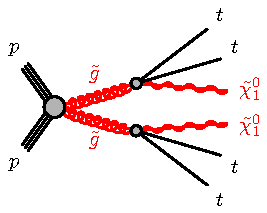
\includegraphics[width=0.24\textwidth]{MODELS/gogo-ttttN1N1}}
\subfigure{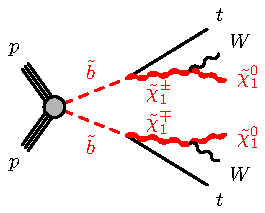
\includegraphics[width=0.24\textwidth]{MODELS/sbsb-ttWWN1N1}}
\caption{Gluino decay via offshell stop (left), and direct sbottom pair production (right).}
\label{fig:feynman_3rdgen}
\end{figure}

\begin{figure}[t]
\centering
\subfigure{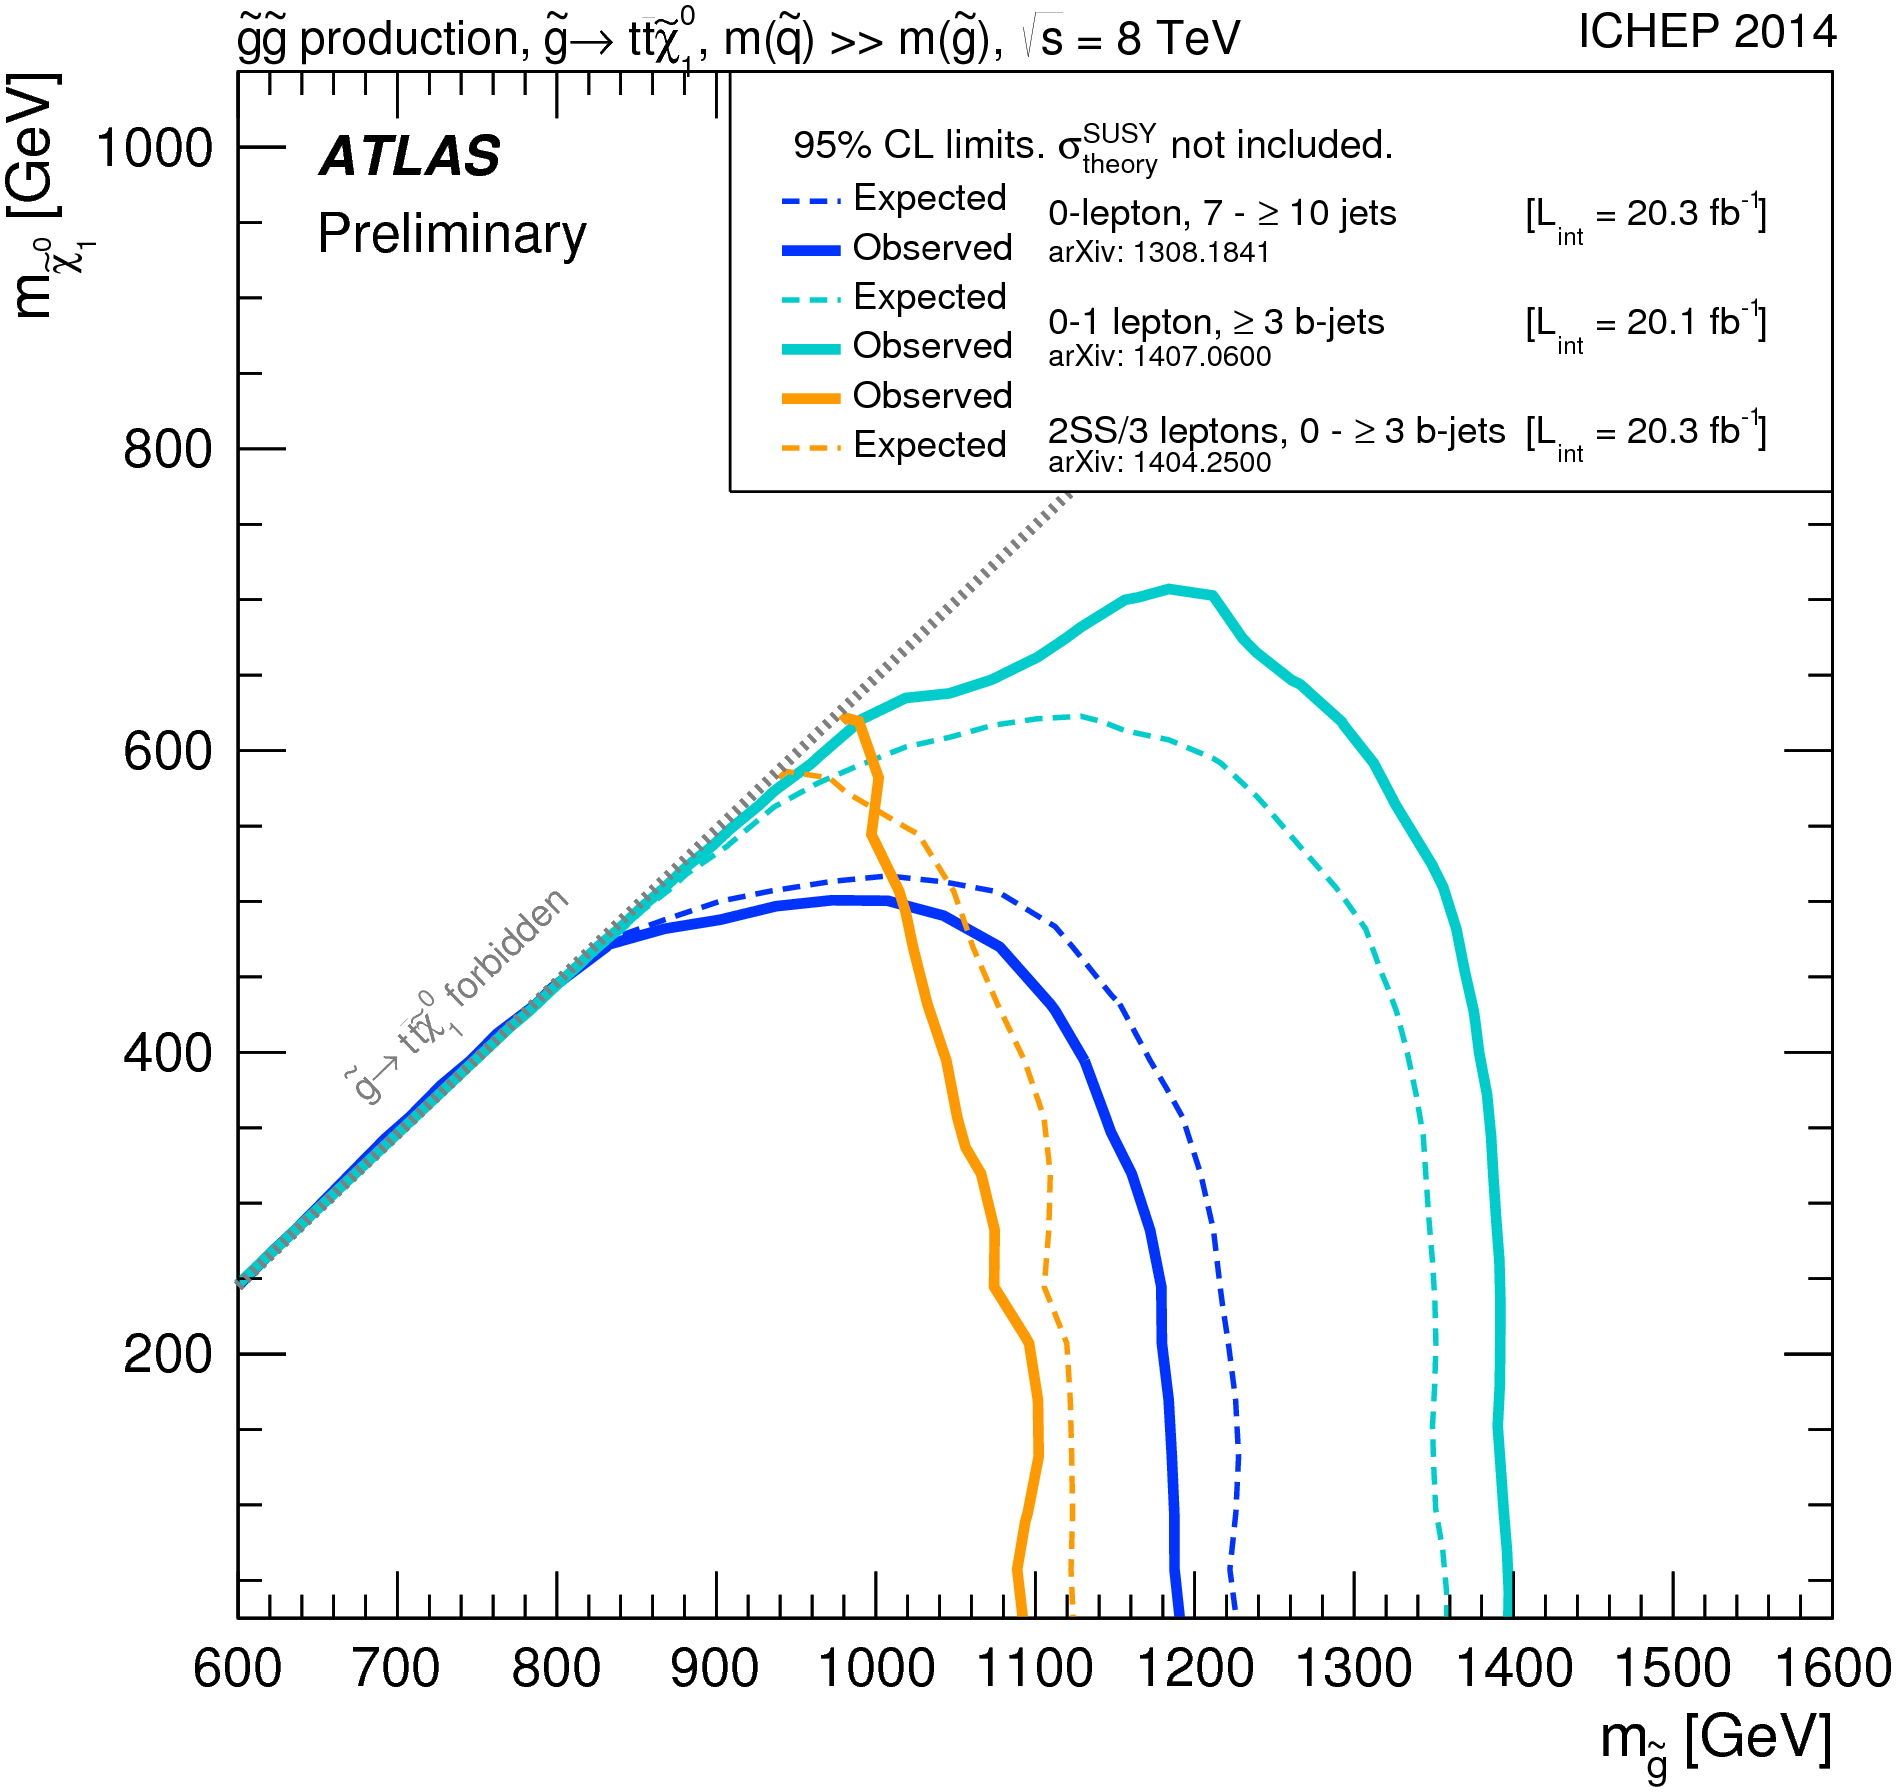
\includegraphics[width=0.49\textwidth]{MODELS/ATLAS_SUSY_Gtt}}
\subfigure{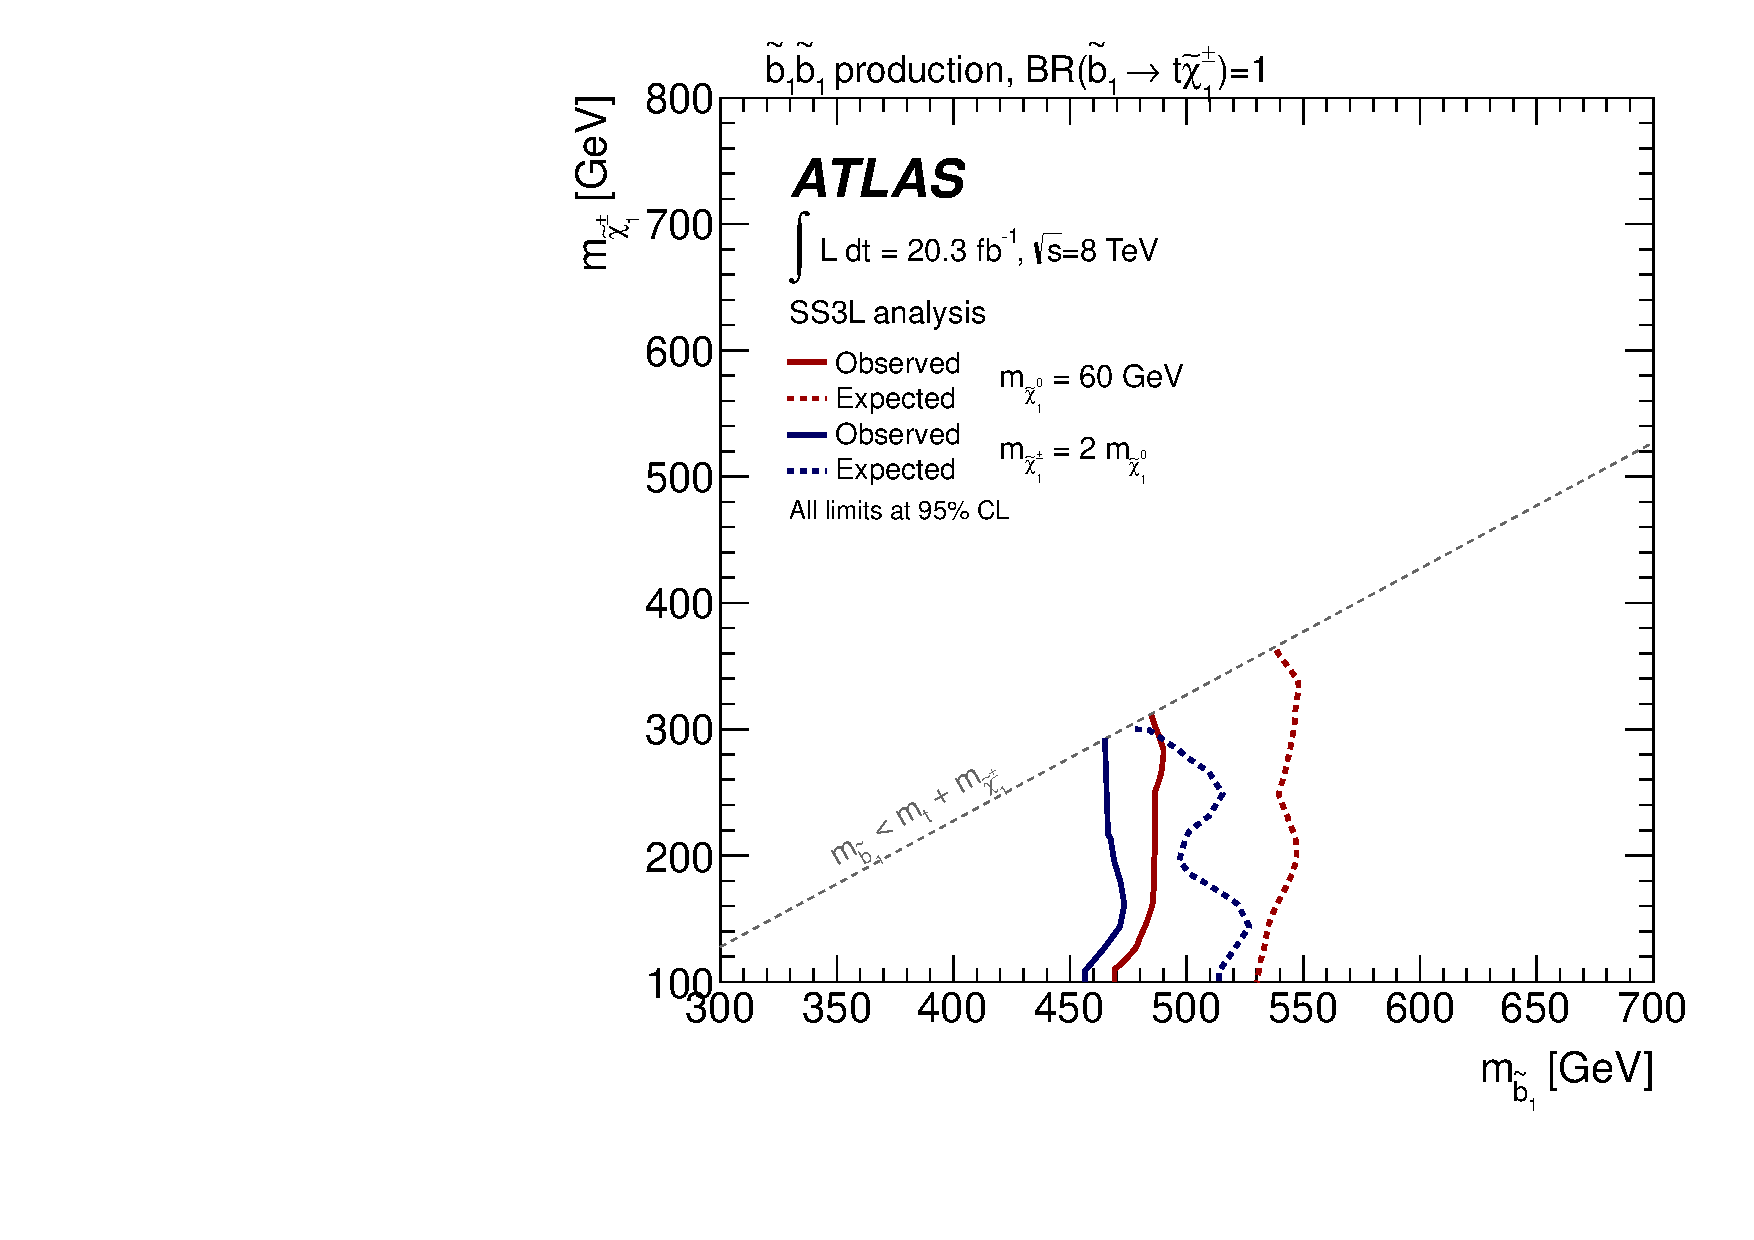
\includegraphics[width=0.49\textwidth]{MODELS/exclusion_sbottom_topC1_both_grids}}
\caption{Exclusion limits on the gluino-stop offshell (left) and direct sbottom (right) scenarios 
set by ATLAS with the 2012 dataset~\cite{DraftSquarkGluinoSummaryPaper}.}
\label{fig:run1excl_3rdgen}
\end{figure}

\par{\bf Gluino-stop offshell $\gluino\to t\bar t\neut$\\}
In this model inspired by naturalness arguments, gluinos are coupling preferentially to stops which are lighter than the other squarks. 
Gluinos are however considered lighter than stops, and decay directly into a $t\bar t\neut$ triplet via a virtual stop (Fig.~\ref{fig:feynman_3rdgen}). 
The pair production of gluinos leads to a final state containing four top quarks and two neutralinos. 
This characteristic final state is accessible through various experimental signatures, which is why this model 
is commonly used as a benchmark to estimate analyses sensitivities. 
The searches performed with run-1 data~\cite{DraftSquarkGluinoSummaryPaper}, 
summarized in Fig.~\ref{fig:run1excl_3rdgen}, showed that the same-sign leptons final state is competitive mainly at large neutralino mass. 
This region of the phase space is consequently given a particular attention in the choice of signal regions described further on. 
In the signal samples referenced in this document, the lightest stop mass is fixed to 10~\TeV and is mostly a $\widetilde{t}_R$ state. 
Only gluino pair production is considered, followed by an exclusive decay in the aforementioned channel. 
\\
\par{\bf Direct sbottom $\sbot\to t\chargino$\\}
In this model, bottom squarks are rather lights and assumed to decay in a top quark and a chargino $\chargino$ (Fig.~\ref{fig:feynman_3rdgen}), 
providing complementarity to the mainstream search which focuses on the channel $\sbot\to b\neut$. 
The final state resulting from the production of a sbottom pair contains pairs of top quarks, of $W$ bosons and of neutralinos. 
While this final state may lead to various experimental signatures, 
the model was considered in run-1~\cite{DraftSquarkGluinoSummaryPaper} 
only by the same-sign leptons and jets search, leading to the exclusion limits presented in Fig.~\ref{fig:run1excl_3rdgen}. 
In the signal samples used by the analysis, the neutralino mass is fixed to 60~\GeV, and the chargino mass to 150~\GeV, while the sbottom mass is varied. 
Only pair production of the lightest sbottom is considered, followed by an exclusive decay in the aforementioned channel. \\


\begin{figure}[h!]
\subfigure{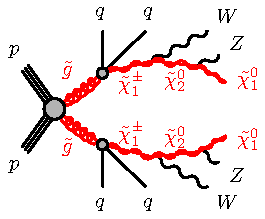
\includegraphics[width=0.24\textwidth]{MODELS/gogo-qqqqWWZZN1N1-C1N2}}
\subfigure{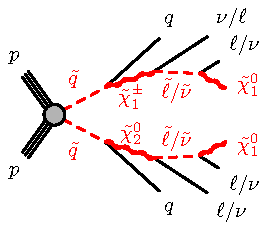
\includegraphics[width=0.24\textwidth]{MODELS/sqsq-qqlllvN1N1-C1N2}}
\subfigure{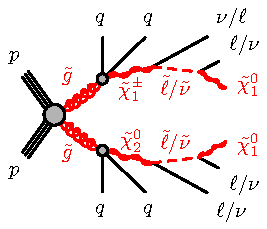
\includegraphics[width=0.24\textwidth]{MODELS/gogo-qqqqlllvN1N1-C1N2}}
\subfigure{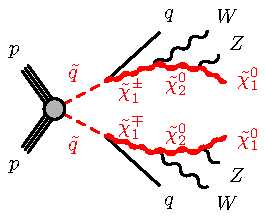
\includegraphics[width=0.24\textwidth]{MODELS/sqsq-qqWWZZN1N1-C1N2}}
\caption{Two-step decays of gluinos and squarks, mediated by gauginos (left) or sleptons (right).}
\label{fig:feynman_1stgen}
\end{figure}

\begin{figure}[t]
\centering
\subfigure{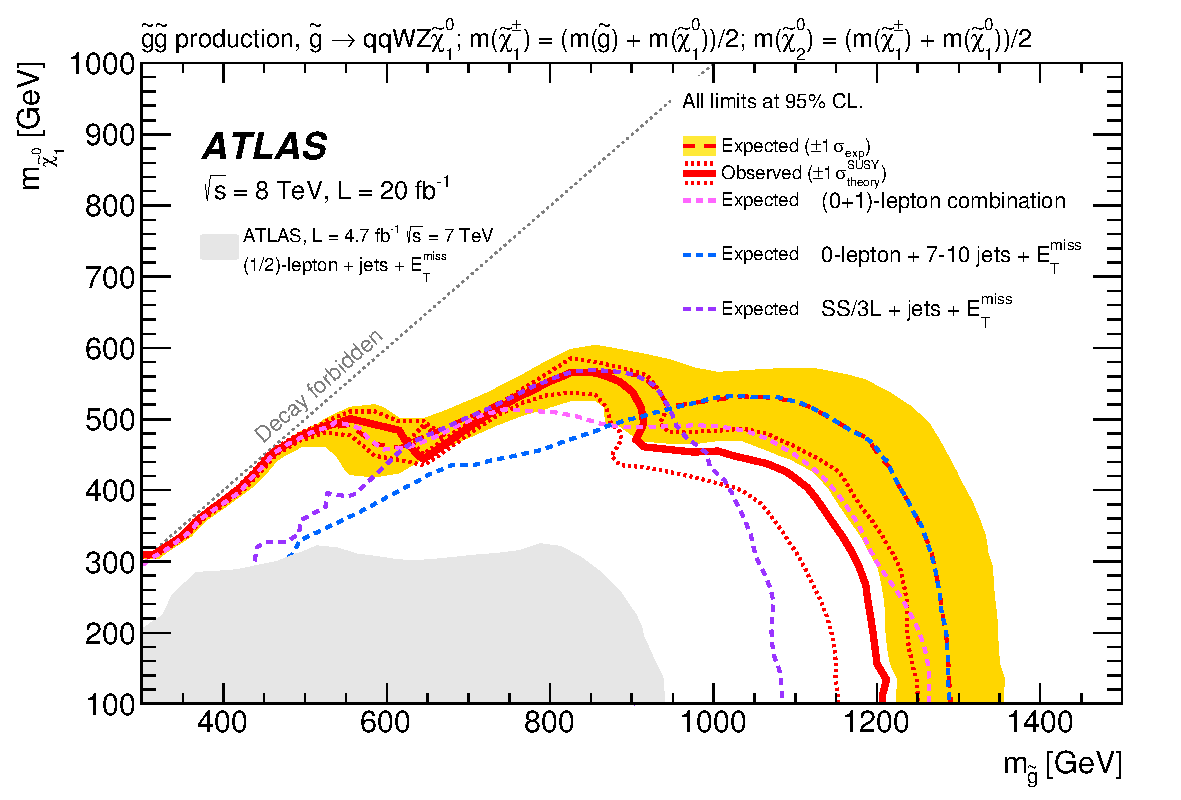
\includegraphics[width=0.49\textwidth]{MODELS/run1excluded_gluino2stepWZ}}
\subfigure{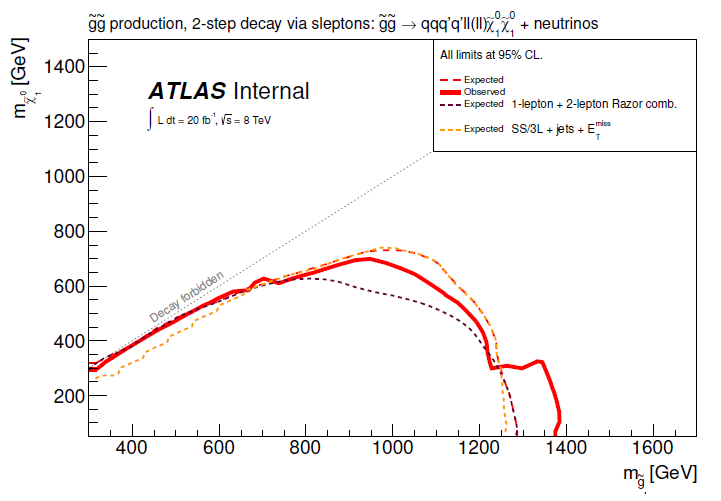
\includegraphics[width=0.49\textwidth]{MODELS/run1excluded_gluino2stepSleptons}}
\subfigure{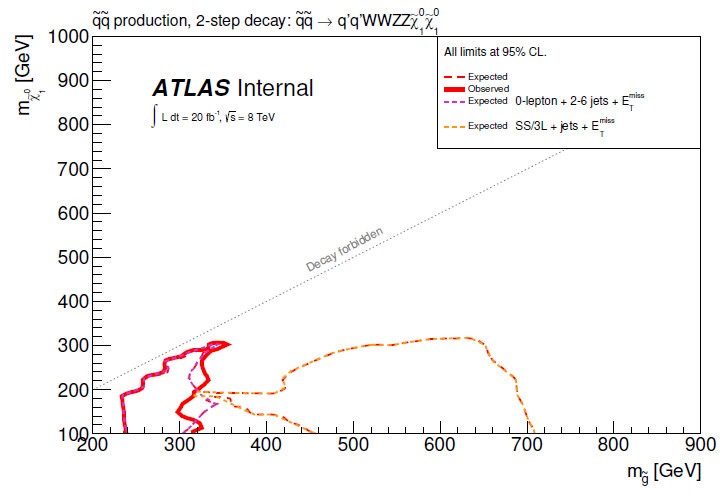
\includegraphics[width=0.49\textwidth]{MODELS/run1excluded_squark2stepWZ}}
\subfigure{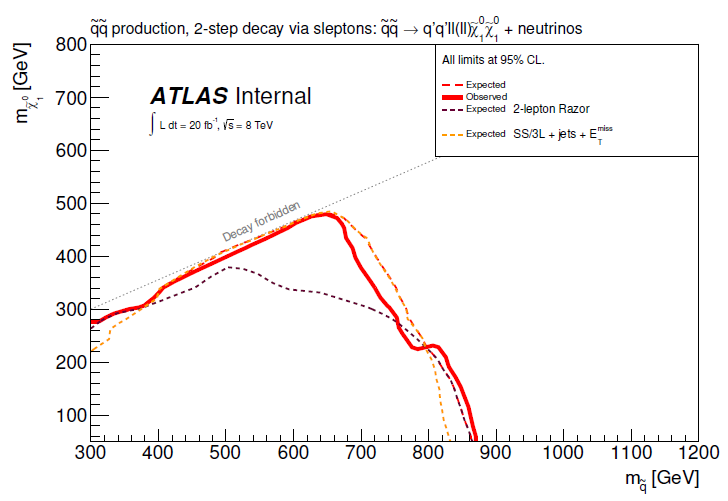
\includegraphics[width=0.49\textwidth]{MODELS/run1excluded_squark2stepSleptons}}
\caption{Exclusion limits on scenarios featuring gluino (top) and squarks (bottom) two-steps decays via gauginos (left) or sleptons (right) 
set by ATLAS with the 2012 dataset~\cite{DraftSquarkGluinoSummaryPaper}.}
\label{fig:run1excluded_1stgen}
\end{figure}

\par{\bf Gluinos and squarks 2-step decays via gauginos\\}
These scenarios feature a less oriented search for gluinos or squarks (save third generation) where gluinos couple preferentially to the latter, 
and squarks decay to charginos (Fig.~\ref{fig:feynman_1stgen} left) with the subsequent cascade $\chargino\to W\tilde{\chi}_{2}^{0} \to WZ\neut$. 
This leads to final states of two light quarks, two $W$ and $Z$ bosons, and two neutralinos 
(with two additional light quarks in the case of gluino pair production). 
Fig.~\ref{fig:run1excluded_1stgen} left shows the exclusion limits obtained with the 2012 dataset~\cite{DraftSquarkGluinoSummaryPaper}; 
in the gluino scenario, the same-sign leptons + jets search provided complementarity at large neutralino mass, 
while its sensitivity in the squark scenario dominated completely. 
In the signal samples used here, the chargino mass is set halfway between the neutralino and squark (or gluino) masses, 
while the neutralino $\tilde{\chi}_{2}^{0}$ mass is set halfway between the chargino and neutralino masses. 
Gluino and squark-antisquark pair production are considered separately in distinct scenarios.  
\\
\par{\bf Gluinos and squarks 2-step decays via sleptons\\}
In these scenarios, gluinos couple preferentially to the squarks of the first two generations, and
the latter decay either to a chargino $\chargino$ or a neutralino $\tilde{\chi}_{2}^{0}$, 
which are assumed to be mass-degenerate, and decay in turn to sleptons (Fig.~\ref{fig:feynman_1stgen} right) 
with $\mathcal{BR}(\chargino\to\nu\tilde\ell) = \mathcal{BR}(\chargino\to\ell\tilde\nu) 
= \mathcal{BR}(\tilde{\chi}_{2}^{0}\to\nu\tilde\nu) = \mathcal{BR}(\tilde{\chi}_{2}^{0}\to\ell\tilde\ell)=50\%$. 
The corresponding final state may contain zero to four charged leptons, neutrinos, two light quarks and two neutralinos 
(with two additional light quarks in the case of gluino pair production). 
Because of the sleptons replacing the gauge bosons featured in the scenarios presented in the previous paragraph, 
these scenarios have comparatively a lower jet multiplicity but a significantly enhanced acceptance in multi-lepton experimental signatures. 
As can be seen on Fig.~\ref{fig:run1excluded_1stgen} right, which presents the exclusion limits obtained with the 2012 dataset~\cite{DraftSquarkGluinoSummaryPaper}, 
the same-sign leptons and jets signature is again very competitive. 
In the signal samples used here, the chargino $\chargino$ and neutralino $\tilde{\chi}_{2}^{0}$ masses are set equal, 
halfway between the neutralino and squark (or gluino) masses, 
while the degenerate sleptons masses are set halfway between these gauginos and the lightest neutralino masses. 
Furthermore, gauginos decay to any slepton flavor with equal probability. 
Gluino and squark-antisquark pair production are considered separately in distinct scenarios. 
\\
\par{\bf Models not considered for the moment\\}
In the publications~\cite{paperSS3L,DraftSquarkGluinoSummaryPaper} of the analysis results obtained with run-1 data, 
exclusion limits were also provided for other signal models, often 
These scenarios included the $\gluino\to tbW\neut$ and $\gluino\to tcW\neut$ simplified models, as well as minimal models featuring 
$R$-parity violation through bilinear terms, gauge-mediated SUSY breaking, or universal extra dimensions. 
These models are not considered here, although interpretations might be proposed for them again in the future. 

\subsection{New models}

%\subsubsection{pMSSM inspired [Sebastien]}

\subsubsection{RPV inspired}
\label{subsec:RPVmodel}

 In supersymmetry, the following superpotential is present :
 \begin{align}
   W = \mu H L + \frac{1}{2} \lambda_{ijk} L_i L_j E_k + \lambda'_{ijk} L_i Q_j D_k + \frac{1}{2} \lambda''_{ijk} U_i D_j D_k
   \label{rpvpotential}
 \end{align}
 where $H$, $L$, $Q$, $E$, $U$ and $D$ are respectively the superpotential associated to the Higgs doublet, the lepton-neutrino doublet, the quark up-down doublet, the right-handed electron, the right-handed up quark and the right-handed down quark.
 The indices $i$, $j$ and $k$ are the flavor indices and $\mu$ , $\lambda_{ijk}$ , $\lambda'_{ijk}$ , $\lambda''_{ijk}$ are the coupling constants.
\\

 The leptonic number violation and the baryonic number violation implied by this potential have an important impact in the physic at low energy
 and do not respect some low energy constraints like the proton decay time limit.
 In $R$-parity conserving (RPC) SUSY models, the $R$-parity is added in order to remove these terms and keep the proton stable.
 However, one can play with the couplings $\mu$ , $\lambda_{ijk}$ , $\lambda'_{ijk}$ and $\lambda''_{ijk}$ in order to violate $R$-parity while respecting the low energy constraints.
 This is called the $R$-parity violation (RPV) SUSY models.
\\

 In this note, we will only consider the case where the coupling constants $\mu$, $\lambda_{ijk}$, $\lambda'_{ijk}$ and $\lambda''_{(i \neq 3) jk}$ are suppressed.
 Therefore, the only non-negligible terms are $\lambda''_{321}TSD$ , $\lambda''_{331}TBD$ and $\lambda''_{323}TSB$ where $T$, $B$, $D$ and $S$ are the superfields associated to the top, bottom, down and strange quark.
 This scenario is predicted by some RPV models like the Minimal Flavor Violation (MFV) scenarios~\cite{Nikolidakis:2007fc,Csaki:2011ge} and leads to the production of same-sign top quarks~\cite{Durieux:2013uqa} (see Fig.~\ref{fig:rpv_diagram}).

\begin{figure}[h!]
\centering
\subfigure{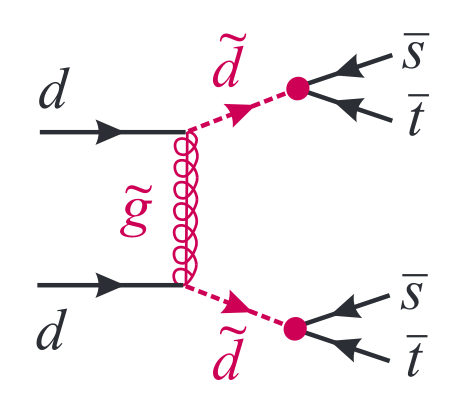
\includegraphics[width=0.24\textwidth]{MODELS/ddfusion.png}}
\subfigure{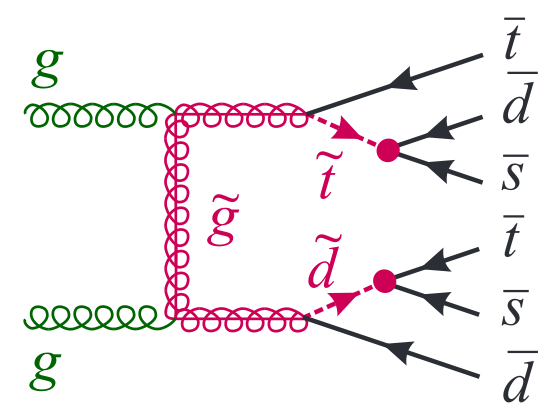
\includegraphics[width=0.27\textwidth]{MODELS/ggfusion.png}}
\caption{Example of diagrams for RPV model for the \textit{d-quark fusion} topology (left), and the \textit{gluon fusion} topology (right) involving the $\lambda''_{321}$ coupling. In both cases, the baryonic number is violated by two units. }
\label{fig:rpv_diagram}
\end{figure}

 In these scenarios, the $R$-parity is not conserved and the LSP is not stable (and therefore cannot be a good dark matter candidate).
 However, the interesting part of this model is that it allows B-violating processes (see Fig.~\ref{fig:rpv_diagram}).
 Actually, the baryonic asymmetry in the universe and the fact that the standard model does not respect this symmetry provides a good motivation for the search for $B$-violation processes at high energy.
 In addition, it was also proved that the violation of the baryonic number by two units involving top quarks could respect the low denergy constraints like the proton decay time limit~\cite{Durieux:2012gj}.
% Therefore, RPV SUSY is good generic model for the search for $B$-violation.
\\

In this analysis, two kind of topologies will be considered:
\begin{itemize}
\item \textbf{d-quark fusion}: Production of two on-shell $d$-squarks with a gluino in $t$-channel and the $d$-squarks decay to an anti-top quark and to one extra jet.
  The squarks will lighter than the gluino and the cross section will mostly depend on the mass of the squark (see Fig.~\ref{fig:rpv_diagram}).
  \begin{align}
    dd \to \tilde{d} \tilde{d}\ ,\ \tilde{d} \to \bar{t}q    
  \end{align}
\item \textbf{gluon fusion}: Production of two on-shell gluinos which decay to a top or an anti-top quark and to two extra jets.
  The gluino will be lighter than the squarks and the cross section will only depend on the mass of the gluino (see Fig.~\ref{fig:rpv_diagram} ).
  \begin{align}
    gg \to \gluino\gluino\ ,\ \gluino \to tqq\ /\ \gluino \to \bar{t}qq'
  \end{align}
\end{itemize}
The extra jets could be either $b$-jet or light jets, depending on the coupling being considered. 
In order to have access to the charge of the top quark, we will only consider the case where the top quark decays leptonically.
At the end, the final states will be composed of two same-sign leptons, at least two $b$-jets, low missing transverse energy (coming from the neutrinos) and extra jets.
\\
% Cross section : soon

 This model was already constrained by ATLAS~\cite{Aad:2014pda} and CMS~\cite{Chatrchyan:2013fea} in Run-1, but those analyses 
 only considered the coupling $\lambda''_{323}$ and the topology of \textit{gluon fusion}.
 A limit of around 900 GeV was found on the mass of the gluino. The full hadronic final state was also exploited in ATLAS~\cite{Aad:2013wta}.



\section{MC samples}
\label{sec:samples}
This section summarizes the signal and background samples used for the
studies presented in this note, as well some details about the Monte Carlo production and analysis framework.
All samples used in this note are part of the DC14 Monte-Carlo campaign which exhibits a number 
of deficiencies~\cite{dc14twiki}, most notably the inaccessibility of detailed trigger information. 

\subsection{Derivation versions and analysis model}
\label{sec:ntuples}

In all cases, the SUSY1 DxAOD derivations are used. 
Derivation tag p1872 (19.1.4.9 cache) is used for most of the samples used in this note, although some signal 
samples were not initially available in that tag and p1863 (19.1.4.8 cache) was used instead. 
Both derivation tags included the fix of lepton isolation 
variables (see Section~\ref{sec:isolation} for more details).

Most of the studies shown in this note were performed using flat ROOT ntuples produced on the grid using code based on the 
{\tt{SUSYAnalysiExample}} EventLoop package and SUSYTools-00-05-00-26 tag. 
They contained basic object information, although no overlap removal 
or isolation cuts were applied to allow flexibility for optimization studies. 
No event skimming or systematic uncertainties were included. 
The total size of these ntuples is 70~GB (both background and signal samples).
These files were shared among the groups participating in the analysis, although some 
of the groups developed their own framework for xAOD analysis.

In addition, dedicated flat ROOT ntuples with all the systematic variations included in the SUSYTools {\tt getSystInfoList()} method 
were also produced for the samples containing prompt SS/3L ($\ttbar+V$, $\ttbar+h$, diboson, signals). To reduce the size of the output files, only events that contained in any of the systematic variations
at least 2 leptons with $\pt>10$~GeV, and either $\et>100$~GeV or at least 3 b-tagged jets ($\pT>20$ GeV) or $H_{\rm T}>300$~GeV were kept.  
In order to benefit from the recently implemented grouping of 
the Egamma systematics, the SUSYTools-00-05-00-29 tag was used for this production, which contains only other minor 
updates with respect to SUSYTools-00-05-00-26. The total size of these ntuples is below 50~GB.


\subsection{Signal Samples}

This section describes the signal samples used for in this note. 
The baseline signal models used are the ones described
in Section~\ref{sec:signal}, and all the signal samples used are listed in Table~\ref{tab:SignalSamples}.

The gluino-stop offshell ($\gluino\to t\bar t\neut$) and direct sbottom ($\sbot\to t\chargino$ with $\tilde{b}_1\to t\tilde{\chi}^{\pm}_1$) samples are produced with {\sc Herwig++}~\cite{Corcella:2000bw}. The UE-EE-4 {\sc Herwig++} tune~\cite{Gieseke:2012ft} is used to describe the underlying event.
%and the generator settings are equivalent to those of the 8 TeV 
%analysis~\cite{noteSS3L} except that the stop mass has been raised to 5
%TeV and the center of mass energy has been adjusted to 13 TeV.
The other signal samples used in this note (gluinos and squarks 2-step decays via gauginos or sleptons) are produced using the {\sc Madgraph v5} generator~\cite{madgraph} using leading-order (LO) matrix elements with up to two additional partons.
{\sc Pythia} 6.425~\cite{Sjostrand:2006za} with the {\sc AUET2B} tune~\cite{pub-2011-009,ATLAS:2011krm} is used for hadronisation and to describe the underlying event. 
In all the signal samples, the {\sc CTEQ6L1}~\cite{Pumplin:2002vw} set of parton distribution functions is used in all the signal samples. The signal samples are normalised to the next-to-next-to-leading order cross-section including the resummation of
soft gluon emission at next-to-next-to-leading-logarithmic accuracy
(NLO+NLL), as detailed in Ref.~\cite{Borschensky:2014cia}. 


\begin{sidewaystable}[htb]
\begin{center}
\resizebox{0.95\textwidth}{!}{
\tiny
\begin{tabular}{lllllll}
\hline
\hline
datasetID & Sample name & $\sigma$ [pb] & $k$-Factor & $\epsilon_{filter}$ & $N_{gen}$ & $L_{equiv}$\\
\hline
\multicolumn{7}{c}{\textbf{Gluino-stop offshell} ($\gluino\to t\bar t\neut$)} \\ \hline
204533  &  mc14\_13TeV.204533.Herwigpp\_UEEE4\_CTEQ6L1\_Gtt\_G1000\_T5000\_L100.merge.DAOD\_SUSY1.e3094\_s1982\_s2008\_r5787\_r5853\_p1872/  &  0.3254  &  1.00  &  1.000  &  20000  &  61.5 \\
204534  &  mc14\_13TeV.204534.Herwigpp\_UEEE4\_CTEQ6L1\_Gtt\_G1300\_T5000\_L100.merge.DAOD\_SUSY1.e3094\_s1982\_s2008\_r5787\_r5853\_p1872/  &  0.0461  &  1.00  &  1.000  &  19500  &  423.0 \\
204535  &  mc14\_13TeV.204535.Herwigpp\_UEEE4\_CTEQ6L1\_Gtt\_G1600\_T5000\_L100.merge.DAOD\_SUSY1.e3094\_s1982\_s2008\_r5787\_r5853\_p1872/  &  0.0081  &  1.00  &  1.000  &  20000  &  2469.1 \\
204536  &  mc14\_13TeV.204536.Herwigpp\_UEEE4\_CTEQ6L1\_Gtt\_G1900\_T5000\_L100.merge.DAOD\_SUSY1.e3094\_s1982\_s2008\_r5787\_r5853\_p1872/  &  0.0016  &  1.00  &  1.000  &  20000  &  12500.0 \\
204537  &  mc14\_13TeV.204537.Herwigpp\_UEEE4\_CTEQ6L1\_Gtt\_G2200\_T5000\_L100.merge.DAOD\_SUSY1.e3094\_s1982\_s2008\_r5787\_r5853\_p1872/  &  0.0004  &  1.00  &  1.000  &  20000  &  50000.0 \\
204539  &  mc14\_13TeV.204539.Herwigpp\_UEEE4\_CTEQ6L1\_Gtt\_G1300\_T5000\_L400.merge.DAOD\_SUSY1.e3094\_s1982\_s2008\_r5787\_r5853\_p1872/  &  0.0461  &  1.00  &  1.000  &  15000  &  325.4 \\
204540  &  mc14\_13TeV.204540.Herwigpp\_UEEE4\_CTEQ6L1\_Gtt\_G1300\_T5000\_L700.merge.DAOD\_SUSY1.e3094\_s1982\_s2008\_r5787\_r5853\_p1872/  &  0.0461  &  1.00  &  1.000  &  20000  &  433.8 \\
204541  &  mc14\_13TeV.204541.Herwigpp\_UEEE4\_CTEQ6L1\_Gtt\_G1300\_T5000\_L900.merge.DAOD\_SUSY1.e3094\_s1982\_s2008\_r5787\_r5853\_p1872/  &  0.0461  &  1.00  &  1.000  &  20000  &  433.8 \\
204912  &  mc14\_13TeV.204912.Herwigpp\_UEEE4\_CTEQ6L1\_Gtt\_G1500\_T5000\_L200.merge.DAOD\_SUSY1.e3328\_s1982\_s2008\_r5787\_r5853\_p1872/  &  0.0142  &  1.00  &  1.000  &  20000  &  1408.5 \\
204913  &  mc14\_13TeV.204913.Herwigpp\_UEEE4\_CTEQ6L1\_Gtt\_G1500\_T5000\_L400.merge.DAOD\_SUSY1.e3328\_s1982\_s2008\_r5787\_r5853\_p1872/  &  0.0142  &  1.00  &  1.000  &  20000  &  1408.5 \\
204914  &  mc14\_13TeV.204914.Herwigpp\_UEEE4\_CTEQ6L1\_Gtt\_G1500\_T5000\_L600.merge.DAOD\_SUSY1.e3328\_s1982\_s2008\_r5787\_r5853\_p1872/  &  0.0142  &  1.00  &  1.000  &  20000  &  1408.5 \\
204915  &  mc14\_13TeV.204915.Herwigpp\_UEEE4\_CTEQ6L1\_Gtt\_G1500\_T5000\_L800.merge.DAOD\_SUSY1.e3328\_s1982\_s2008\_r5787\_r5853\_p1872/  &  0.0142  &  1.00  &  1.000  &  20000  &  1408.5 \\
204916  &  mc14\_13TeV.204916.Herwigpp\_UEEE4\_CTEQ6L1\_Gtt\_G1500\_T5000\_L1000.merge.DAOD\_SUSY1.e3328\_s1982\_s2008\_r5787\_r5853\_p1872/  &  0.0142  &  1.00  &  1.000  &  20000  &  1408.5 \\ \hline
\multicolumn{7}{c}{\textbf{Direct sbottom} ($\sbot\to t\chargino$ with $\tilde{b}_1\to t\tilde{\chi}^{\pm}_1$)} \\ \hline
204973  &  mc14\_13TeV.204973.Herwigpp\_UEEE4\_CTEQ6L1\_sbottom\_tchr\_2lep\_B450\_C150\_N60.merge.DAOD\_SUSY1.e3356\_s1982\_s2008\_r5787\_r5853\_p1863/  &  0.9483  &  0.41  &  0.409  &  20000  &  125.8 \\
204974  &  mc14\_13TeV.204974.Herwigpp\_UEEE4\_CTEQ6L1\_sbottom\_tchr\_2lep\_B550\_C150\_N60.merge.DAOD\_SUSY1.e3356\_s1982\_s2008\_r5787\_r5853\_p1863/  &  0.2961  &  0.43  &  0.432  &  11000  &  200.0 \\
204975  &  mc14\_13TeV.204975.Herwigpp\_UEEE4\_CTEQ6L1\_sbottom\_tchr\_2lep\_B650\_C150\_N60.merge.DAOD\_SUSY1.e3356\_s1982\_s2008\_r5787\_r5853\_p1863/  &  0.1070  &  0.45  &  0.451  &  20000  &  921.0 \\
204976  &  mc14\_13TeV.204976.Herwigpp\_UEEE4\_CTEQ6L1\_sbottom\_tchr\_2lep\_B750\_C150\_N60.merge.DAOD\_SUSY1.e3356\_s1982\_s2008\_r5787\_r5853\_p1863/  &  0.0431  &  0.47  &  0.472  &  20000  &  2091.8 \\
204977  &  mc14\_13TeV.204977.Herwigpp\_UEEE4\_CTEQ6L1\_sbottom\_tchr\_2lep\_B850\_C150\_N60.merge.DAOD\_SUSY1.e3356\_s1982\_s2008\_r5787\_r5853\_p1863/  &  0.0190  &  0.48  &  0.483  &  20000  &  4540.3 \\
\hline
\multicolumn{7}{c}{\textbf{gluino 2-step decays via gauginos}} \\ \hline
204952  &  mc14\_13TeV.204952.MadGraphPythia\_AUET2BCTEQ6L1\_SMGG2WWZZ\_1100\_600\_100.merge.DAOD\_SUSY1.e3345\_s1982\_s2008\_r5787\_r5853\_p1872/  &  0.1635  &  1.00  &  1.000  &  19500  &  119.3 \\
204953  &  mc14\_13TeV.204953.MadGraphPythia\_AUET2BCTEQ6L1\_SMGG2WWZZ\_1300\_700\_100.merge.DAOD\_SUSY1.e3345\_s1982\_s2008\_r5787\_r5853\_p1872/  &  0.0461  &  1.00  &  1.000  &  5000  &  108.5 \\
204954  &  mc14\_13TeV.204954.MadGraphPythia\_AUET2BCTEQ6L1\_SMGG2WWZZ\_1500\_800\_100.merge.DAOD\_SUSY1.e3345\_s1982\_s2008\_r5787\_r5853\_p1872/  &  0.0142  &  1.00  &  1.000  &  20000  &  1408.5 \\
204955  &  mc14\_13TeV.204955.MadGraphPythia\_AUET2BCTEQ6L1\_SMGG2WWZZ\_1700\_900\_100.merge.DAOD\_SUSY1.e3345\_s1982\_s2008\_r5787\_r5853\_p1872/  &  0.0047  &  1.00  &  1.000  &  15000  &  3191.5 \\
204956  &  mc14\_13TeV.204956.MadGraphPythia\_AUET2BCTEQ6L1\_SMGG2WWZZ\_1900\_1000\_100.merge.DAOD\_SUSY1.e3345\_s1982\_s2008\_r5787\_r5853\_p1872/  &  0.0016  &  1.00  &  1.000  &  15500  &  9687.5 \\
204957  &  mc14\_13TeV.204957.MadGraphPythia\_AUET2BCTEQ6L1\_SMGG2WWZZ\_2100\_1100\_100.merge.DAOD\_SUSY1.e3345\_s1982\_s2008\_r5787\_r5853\_p1872/  &  0.0006  &  1.00  &  1.000  &  5000  &  8333.3 \\
204958  &  mc14\_13TeV.204958.MadGraphPythia\_AUET2BCTEQ6L1\_SMGG2WWZZ\_2300\_1200\_100.merge.DAOD\_SUSY1.e3345\_s1982\_s2008\_r5787\_r5853\_p1872/  &  0.0002  &  1.00  &  1.000  &  13500  &  67500.0 \\
204959  &  mc14\_13TeV.204959.MadGraphPythia\_AUET2BCTEQ6L1\_SMGG2WWZZ\_1000\_700\_400.merge.DAOD\_SUSY1.e3345\_s1982\_s2008\_r5787\_r5853\_p1872/  &  0.3254  &  1.00  &  1.000  &  5000  &  15.4 \\
204960  &  mc14\_13TeV.204960.MadGraphPythia\_AUET2BCTEQ6L1\_SMGG2WWZZ\_1000\_750\_500.merge.DAOD\_SUSY1.e3345\_s1982\_s2008\_r5787\_r5853\_p1872/  &  0.3254  &  1.00  &  1.000  &  7500  &  23.0 \\
204961  &  mc14\_13TeV.204961.MadGraphPythia\_AUET2BCTEQ6L1\_SMGG2WWZZ\_1000\_800\_600.merge.DAOD\_SUSY1.e3345\_s1982\_s2008\_r5787\_r5853\_p1872/  &  0.3254  &  1.00  &  1.000  &  20000  &  61.5 \\
204962  &  mc14\_13TeV.204962.MadGraphPythia\_AUET2BCTEQ6L1\_SMGG2WWZZ\_1000\_850\_700.merge.DAOD\_SUSY1.e3345\_s1982\_s2008\_r5787\_r5853\_p1872/  &  0.3254  &  1.00  &  1.000  &  20000  &  61.5 \\
204963  &  mc14\_13TeV.204963.MadGraphPythia\_AUET2BCTEQ6L1\_SMGG2WWZZ\_1000\_900\_800.merge.DAOD\_SUSY1.e3345\_s1982\_s2008\_r5787\_r5853\_p1872/  &  0.3254  &  1.00  &  1.000  &  20000  &  61.5 \\
204964  &  mc14\_13TeV.204964.MadGraphPythia\_AUET2BCTEQ6L1\_SMGG2WWZZ\_1000\_950\_900.merge.DAOD\_SUSY1.e3345\_s1982\_s2008\_r5787\_r5853\_p1872/  &  0.3254  &  1.00  &  1.000  &  10000  &  30.7 \\
\hline
\multicolumn{7}{c}{\textbf{squark 2-step decays via gauginos}} \\ \hline
204965  &  mc14\_13TeV.204965.MadGraphPythia\_AUET2BCTEQ6L1\_SMSS2WWZZ\_650\_375\_100.merge.DAOD\_SUSY1.e3345\_s1982\_s2008\_r5787\_r5853\_p1872/  &  0.0695  &  1.00  &  1.000  &  5000  &  71.9 \\
204966  &  mc14\_13TeV.204966.MadGraphPythia\_AUET2BCTEQ6L1\_SMSS2WWZZ\_750\_425\_100.merge.DAOD\_SUSY1.e3345\_s1982\_s2008\_r5787\_r5853\_p1872/  &  0.0219  &  1.00  &  1.000  &  20000  &  913.2 \\
204967  &  mc14\_13TeV.204967.MadGraphPythia\_AUET2BCTEQ6L1\_SMSS2WWZZ\_850\_475\_100.merge.DAOD\_SUSY1.e3345\_s1982\_s2008\_r5787\_r5853\_p1872/  &  0.0075  &  1.00  &  1.000  &  17500  &  2333.3 \\
204968  &  mc14\_13TeV.204968.MadGraphPythia\_AUET2BCTEQ6L1\_SMSS2WWZZ\_950\_525\_100.merge.DAOD\_SUSY1.e3345\_s1982\_s2008\_r5787\_r5853\_p1872/  &  0.0027  &  1.00  &  1.000  &  19000  &  7037.0 \\
204969  &  mc14\_13TeV.204969.MadGraphPythia\_AUET2BCTEQ6L1\_SMSS2WWZZ\_650\_475\_300.merge.DAOD\_SUSY1.e3345\_s1982\_s2008\_r5787\_r5853\_p1872/  &  0.0695  &  1.00  &  1.000  &  20000  &  287.8 \\
204970  &  mc14\_13TeV.204970.MadGraphPythia\_AUET2BCTEQ6L1\_SMSS2WWZZ\_650\_525\_400.merge.DAOD\_SUSY1.e3345\_s1982\_s2008\_r5787\_r5853\_p1872/  &  0.0695  &  1.00  &  1.000  &  20000  &  287.8 \\
204971  &  mc14\_13TeV.204971.MadGraphPythia\_AUET2BCTEQ6L1\_SMSS2WWZZ\_650\_575\_500.merge.DAOD\_SUSY1.e3345\_s1982\_s2008\_r5787\_r5853\_p1872/  &  0.0695  &  1.00  &  1.000  &  20000  &  287.8 \\
204972  &  mc14\_13TeV.204972.MadGraphPythia\_AUET2BCTEQ6L1\_SMSS2WWZZ\_650\_625\_600.merge.DAOD\_SUSY1.e3345\_s1982\_s2008\_r5787\_r5853\_p1872/  &  0.0695  &  1.00  &  1.000  &  20000  &  287.8 \\
\hline
\hline
\end{tabular}}
\end{center}
\caption{List of simulated samples for the signal models used in this note. The dataset ID, the 
  cross-section $\sigma$, the $k$-Factor, the generator filter
  efficiency $\epsilon_{filter}$, the total number of
  generated events $N_{gen}$ and the equivalent luminosity ($L_{equiv}$) are shown.}
\label{tab:SignalSamples}
\end{sidewaystable}



\subsection{Background Samples}
\label{sec:BGSamples}

All the background samples used are listed in Tables~\ref{tab:BGSamples1}-\ref{tab:BGSamples3}.

Simulated $t\bar{t}$ events are generated using the {\sc Powheg} generator
version r2330.2 ~\cite{Nason:2004rx,Frixione:2007vw,Alioli:2010xd}, which implements
the next-to-leading order matrix element for inclusive $t\bar{t}$
production and uses the
CT10 PDF set~\cite{Lai:2010vv}. {\sc Powheg} is interfaced to {\sc Pythia} 6.427~\cite{Sjostrand:2006za}
with the CTEQ6L1 PDF set using the
Perugia2012 tune~\cite{Skands:2010ak}. The $t\bar{t}$ samples are normalised to their
next-to-next-to-leading order cross-section including the resummation of
soft gluon emission at next-to-next-to-leading-logarithmic accuracy
using Top++2.0 ~\cite{Czakon:2011xx}.

Simulated $W$/$Z$+jets samples are produced using {\sc Sherpa} 1.4.5
~\cite{gleisberg:2008ta} with massive $b$-, $c$-quarks with up to four
additional partons in the matrix element and parton shower and are
normalised to their next-to-next-to-leading order QCD theoretical
cross sections~\cite{Catani:2009sm}.

Samples of single top quark backgrounds corresponding to the $t$-, $s$-
and $Wt$ production mechanisms are generated with {\sc Powheg} version r2330.2
using the CT10 PDF set. All single-top samples are interfaced to {\sc Pythia} 6.427
with the CTEQ6L1 set of parton distribution functions using the
Perugia2012 tune. The leading-order cross-sections obtained from the
generator is used for these samples.

The processes of $t\bar{t}+V$ production are generated with {\sc MadGraph} 5
2.1.1~\cite{madgraph} + {\sc Pythia} 6.427 using the CTEQ6L1 set of parton
distribution functions and the AUET2B underlying event
tune~\cite{ATLAS:2011krm}. The samples are normalised to their
next-to-leading order cross-sections using the $k$-factors computed for $\sqrt{s}=14$~TeV~\cite{Campbell:2012dh,Kardos:2011na}. 

% 
Simulated samples for diboson processes are simulated with {\sc Sherpa} 1.4.5 ($WZ/ZZ\to\ell\ell\nu\nu$ and $W^{\pm}W^{\pm}jj\to\ell^{\pm}\ell^{\pm}\nu\nu jj$ electroweak production), {\sc Powheg} r2330.3 + {\sc Pythia 8} ($WW$, $WZ$ and $ZZ$) and {\tt gg2VV}~\cite{Kauer:2013qba,Kauer:2012hd} in {\sc Powheg} r2330.3 + {\sc Pythia 8} ($gg\to h\to WW$).

QCD multijets are not included in this study since these
backgrounds are expected to be very small.
Note that some background processes that had a non-negligible (despite small) contribution to the analysis in Run-1,
such as tri-boson or $t+Z$ production, were not included in the DC14 productions.

% Processes involving Higgs production are generated with PYTHIA8.
\begin{sidewaystable}[h]
\begin{center}
\resizebox{0.9\textwidth}{!}{
\tiny
\begin{tabular}{lllllll}
\hline
\hline
datasetID & Sample name & $\sigma$ [pb] & $k$-Factor & $\epsilon_{filter}$ & $N_{gen}$ & $L_{equiv}$\\
\hline
110401  &  mc14\_13TeV.110401.PowhegPythia\_P2012\_ttbar\_nonallhad.merge.DAOD\_SUSY1.e2928\_s1982\_s2008\_r5787\_r5853\_p1872/  &  831.7600  &  1.00  &  0.543  &  9970500  &  22.1 \\
119353  &  mc14\_13TeV.119353.MadGraphPythia\_AUET2BCTEQ6L1\_ttbarW.merge.DAOD\_SUSY1.e3214\_s1982\_s2008\_r5787\_r5853\_p1872/  &  0.2014  &  1.22  &  1.000  &  399500  &  1625.9 \\
119355  &  mc14\_13TeV.119355.MadGraphPythia\_AUET2BCTEQ6L1\_ttbarZ.merge.DAOD\_SUSY1.e3214\_s1982\_s2008\_r5787\_r5853\_p1872/  &  0.1857  &  1.56  &  1.000  &  400000  &  1380.8 \\
119583  &  mc14\_13TeV.119583.MadgraphPythia\_AUET2B\_CTEQ6L1\_ttbarWW.merge.DAOD\_SUSY1.e3214\_s1982\_s2008\_r5787\_r5853\_p1872/  &  0.0030  &  1.00  &  1.000  &  10000  &  3333.3 \\
174830  &  mc14\_13TeV.174830.MadGraphPythia\_AUET2BCTEQ6L1\_ttbarWjExcl.merge.DAOD\_SUSY1.e3214\_s1982\_s2008\_r5787\_r5853\_p1872/  &  0.1313  &  1.22  &  1.000  &  399500  &  2494.0 \\
174831  &  mc14\_13TeV.174831.MadGraphPythia\_AUET2BCTEQ6L1\_ttbarWjjIncl.merge.DAOD\_SUSY1.e3214\_s1982\_s2008\_r5787\_r5853\_p1872/  &  0.1627  &  1.22  &  1.000  &  395000  &  1990.0 \\
174832  &  mc14\_13TeV.174832.MadGraphPythia\_AUET2BCTEQ6L1\_ttbarZjExcl.merge.DAOD\_SUSY1.e3214\_s1982\_s2008\_r5787\_r5853\_p1872/  &  0.1663  &  1.56  &  1.000  &  399500  &  1539.9 \\
174833  &  mc14\_13TeV.174833.MadGraphPythia\_AUET2BCTEQ6L1\_ttbarZjjIncl.merge.DAOD\_SUSY1.e3214\_s1982\_s2008\_r5787\_r5853\_p1872/  &  0.2076  &  1.56  &  1.000  &  399500  &  1233.6 \\
110070  &  mc14\_13TeV.110070.PowhegPythia\_P2012\_singletop\_tchan\_lept\_top.merge.DAOD\_SUSY1.e3049\_s1982\_s2008\_r5787\_r5853\_p1872/  &  43.7550  &  1.00  &  1.000  &  999000  &  22.8 \\

110071  &  mc14\_13TeV.110071.PowhegPythia\_P2012\_singletop\_tchan\_lept\_antitop.merge.DAOD\_SUSY1.e3049\_s1982\_s2008\_r5787\_r5853\_p1872/  &  25.7780  &  1.00  &  1.000  &  1000000  &  38.8 \\

110302  &  mc14\_13TeV.110302.PowhegPythia\_P2012\_st\_schan\_lep.merge.DAOD\_SUSY1.e3049\_s1982\_s2008\_r5787\_r5853\_p1872/  &  3.3514  &  1.00  &  1.000  &  999500  &  298.2 \\

110305  &  mc14\_13TeV.110305.PowhegPythia\_P2012\_st\_Wtchan\_incl\_DR.merge.DAOD\_SUSY1.e3049\_s1982\_s2008\_r5787\_r5853\_p1872/  &  68.4590  &  1.00  &  1.000  &  958500  &  14.0 \\
%\hline
%161105 & mc14\_13TeV.161105.Pythia8\_AU2CTEQ6L1\_WH125\_WW2lep.merge.DAOD\_SUSY1.e2743\_s1982\_s2008\_r5787\_r5853\_p1872/ & 0.24 & 1.00 & 0.104 & 0.025 & 100000  \\ 
%161155 & mc14\_13TeV.161155.Pythia8\_AU2CTEQ6L1\_ZH125\_WW2lep.merge.DAOD\_SUSY1.e2743\_s1982\_s2008\_r5787\_r5853\_p1872/ & 0.01 & 1.00 & 1.000 & 0.014 & 100000  \\ 
%161305 & mc14\_13TeV.161305.Pythia8\_AU2CTEQ6L1\_ttH125\_WWinclusive.merge.DAOD\_SUSY1.e2743\_s1982\_s2008\_r5787\_r5853\_p1872/ & 0.07 & 1.00 & 1.000 & 0.071 & 199500  \\ 
\hline
167740  &  mc14\_13TeV.167740.Sherpa\_CT10\_WenuMassiveCBPt0\_BFilter.merge.DAOD\_SUSY1.e2822\_s1982\_s2008\_r5787\_r5853\_p1872/  &  18795.0000  &  1.07  &  0.018  &  497000  &  1.4 \\
167741  &  mc14\_13TeV.167741.Sherpa\_CT10\_WenuMassiveCBPt0\_CJetFilterBVeto.merge.DAOD\_SUSY1.e2822\_s1982\_s2008\_r5787\_r5853\_p1872/  &  18804.0000  &  1.07  &  0.063  &  494500  &  0.4 \\
167742  &  mc14\_13TeV.167742.Sherpa\_CT10\_WenuMassiveCBPt0\_CJetVetoBVeto.merge.DAOD\_SUSY1.e2822\_s1982\_s2008\_r5787\_r5853\_p1872/  &  18843.0000  &  1.07  &  0.919  &  1000000  &  0.1 \\
167743  &  mc14\_13TeV.167743.Sherpa\_CT10\_WmunuMassiveCBPt0\_BFilter.merge.DAOD\_SUSY1.e2822\_s1982\_s2008\_r5787\_r5853\_p1872/  &  18793.0000  &  1.07  &  0.018  &  499500  &  1.4 \\
167744  &  mc14\_13TeV.167744.Sherpa\_CT10\_WmunuMassiveCBPt0\_CJetFilterBVeto.merge.DAOD\_SUSY1.e2822\_s1982\_s2008\_r5787\_r5853\_p1872/  &  18788.0000  &  1.07  &  0.056  &  498000  &  0.4 \\
167745  &  mc14\_13TeV.167745.Sherpa\_CT10\_WmunuMassiveCBPt0\_CJetVetoBVeto.merge.DAOD\_SUSY1.e2822\_s1982\_s2008\_r5787\_r5853\_p1872/  &  18797.0000  &  1.07  &  0.926  &  989500  &  0.1 \\
167746  &  mc14\_13TeV.167746.Sherpa\_CT10\_WtaunuMassiveCBPt0\_BFilter.merge.DAOD\_SUSY1.e2822\_s1982\_s2008\_r5787\_r5853\_p1872/  &  18795.0000  &  1.07  &  0.018  &  500000  &  1.4 \\
167747  &  mc14\_13TeV.167747.Sherpa\_CT10\_WtaunuMassiveCBPt0\_CJetFilterBVeto.merge.DAOD\_SUSY1.e2822\_s1982\_s2008\_r5787\_r5853\_p1872/  &  18808.0000  &  1.07  &  0.060  &  500000  &  0.4 \\
167748  &  mc14\_13TeV.167748.Sherpa\_CT10\_WtaunuMassiveCBPt0\_CJetVetoBVeto.merge.DAOD\_SUSY1.e2822\_s1982\_s2008\_r5787\_r5853\_p1872/  &  18800.0000  &  1.07  &  0.923  &  499500  &  0.0 \\
167761  &  mc14\_13TeV.167761.Sherpa\_CT10\_WenuMassiveCBPt70\_140\_BFilter.merge.DAOD\_SUSY1.e2822\_s1982\_s2008\_r5787\_r5853\_p1872/  &  557.8700  &  1.07  &  0.055  &  349500  &  10.6 \\
167762  &  mc14\_13TeV.167762.Sherpa\_CT10\_WenuMassiveCBPt70\_140\_CJetFilterBVeto.merge.DAOD\_SUSY1.e2822\_s1982\_s2008\_r5787\_r5853\_p1872/  &  557.9200  &  1.07  &  0.227  &  350000  &  2.6 \\
167763  &  mc14\_13TeV.167763.Sherpa\_CT10\_WenuMassiveCBPt70\_140\_CJetVetoBVeto.merge.DAOD\_SUSY1.e2822\_s1982\_s2008\_r5787\_r5853\_p1872/  &  558.3700  &  1.07  &  0.718  &  985500  &  2.3 \\
167764  &  mc14\_13TeV.167764.Sherpa\_CT10\_WmunuMassiveCBPt70\_140\_BFilter.merge.DAOD\_SUSY1.e2822\_s1982\_s2008\_r5787\_r5853\_p1872/  &  557.8700  &  1.07  &  0.055  &  345500  &  10.5 \\
167765  &  mc14\_13TeV.167765.Sherpa\_CT10\_WmunuMassiveCBPt70\_140\_CJetFilterBVeto.merge.DAOD\_SUSY1.e2822\_s1982\_s2008\_r5787\_r5853\_p1872/  &  558.2500  &  1.07  &  0.220  &  350000  &  2.7 \\
167766  &  mc14\_13TeV.167766.Sherpa\_CT10\_WmunuMassiveCBPt70\_140\_CJetVetoBVeto.merge.DAOD\_SUSY1.e2822\_s1982\_s2008\_r5787\_r5853\_p1872/  &  557.4800  &  1.07  &  0.724  &  500000  &  1.2 \\
167767  &  mc14\_13TeV.167767.Sherpa\_CT10\_WtaunuMassiveCBPt70\_140\_BFilter.merge.DAOD\_SUSY1.e2822\_s1982\_s2008\_r5787\_r5853\_p1872/  &  557.9200  &  1.07  &  0.055  &  349500  &  10.6 \\
167768  &  mc14\_13TeV.167768.Sherpa\_CT10\_WtaunuMassiveCBPt70\_140\_CJetFilterBVeto.merge.DAOD\_SUSY1.e2822\_s1982\_s2008\_r5787\_r5853\_p1872/  &  557.6800  &  1.07  &  0.224  &  349500  &  2.6 \\
167769  &  mc14\_13TeV.167769.Sherpa\_CT10\_WtaunuMassiveCBPt70\_140\_CJetVetoBVeto.merge.DAOD\_SUSY1.e2822\_s1982\_s2008\_r5787\_r5853\_p1872/  &  558.5900  &  1.07  &  0.720  &  999500  &  2.3 \\
167770  &  mc14\_13TeV.167770.Sherpa\_CT10\_WenuMassiveCBPt140\_280\_BFilter.merge.DAOD\_SUSY1.e2822\_s1982\_s2008\_r5787\_r5853\_p1872/  &  81.8640  &  1.07  &  0.075  &  198000  &  30.1 \\
167771  &  mc14\_13TeV.167771.Sherpa\_CT10\_WenuMassiveCBPt140\_280\_CJetFilterBVeto.merge.DAOD\_SUSY1.e2822\_s1982\_s2008\_r5787\_r5853\_p1872/  &  81.9180  &  1.07  &  0.255  &  200000  &  8.9 \\
167772  &  mc14\_13TeV.167772.Sherpa\_CT10\_WenuMassiveCBPt140\_280\_CJetVetoBVeto.merge.DAOD\_SUSY1.e2822\_s1982\_s2008\_r5787\_r5853\_p1872/  &  81.7640  &  1.07  &  0.671  &  398000  &  6.8 \\
167773  &  mc14\_13TeV.167773.Sherpa\_CT10\_WmunuMassiveCBPt140\_280\_BFilter.merge.DAOD\_SUSY1.e2822\_s1982\_s2008\_r5787\_r5853\_p1872/  &  81.7750  &  1.07  &  0.074  &  349500  &  54.0 \\
167774  &  mc14\_13TeV.167774.Sherpa\_CT10\_WmunuMassiveCBPt140\_280\_CJetFilterBVeto.merge.DAOD\_SUSY1.e2822\_s1982\_s2008\_r5787\_r5853\_p1872/  &  81.8130  &  1.07  &  0.250  &  349000  &  15.9 \\
167775  &  mc14\_13TeV.167775.Sherpa\_CT10\_WmunuMassiveCBPt140\_280\_CJetVetoBVeto.merge.DAOD\_SUSY1.e2822\_s1982\_s2008\_r5787\_r5853\_p1872/  &  81.9250  &  1.07  &  0.676  &  999500  &  16.9 \\
167776  &  mc14\_13TeV.167776.Sherpa\_CT10\_WtaunuMassiveCBPt140\_280\_BFilter.merge.DAOD\_SUSY1.e2822\_s1982\_s2008\_r5787\_r5853\_p1872/  &  81.8670  &  1.07  &  0.075  &  200000  &  30.4 \\
167777  &  mc14\_13TeV.167777.Sherpa\_CT10\_WtaunuMassiveCBPt140\_280\_CJetFilterBVeto.merge.DAOD\_SUSY1.e2822\_s1982\_s2008\_r5787\_r5853\_p1872/  &  81.7000  &  1.07  &  0.253  &  199927  &  9.0 \\
167778  &  mc14\_13TeV.167778.Sherpa\_CT10\_WtaunuMassiveCBPt140\_280\_CJetVetoBVeto.merge.DAOD\_SUSY1.e2822\_s1982\_s2008\_r5787\_r5853\_p1872/  &  81.7680  &  1.07  &  0.673  &  400000  &  6.8 \\
167779  &  mc14\_13TeV.167779.Sherpa\_CT10\_WenuMassiveCBPt280\_500\_BFilter.merge.DAOD\_SUSY1.e2822\_s1982\_s2008\_r5787\_r5853\_p1872/  &  6.2271  &  1.00  &  0.098  &  399500  &  654.6 \\
167780  &  mc14\_13TeV.167780.Sherpa\_CT10\_WenuMassiveCBPt280\_500\_CJetFilterBVeto.merge.DAOD\_SUSY1.e2822\_s1982\_s2008\_r5787\_r5853\_p1872/  &  6.2128  &  1.07  &  0.273  &  99500  &  54.8 \\
167781  &  mc14\_13TeV.167781.Sherpa\_CT10\_WenuMassiveCBPt280\_500\_CJetVetoBVeto.merge.DAOD\_SUSY1.e2822\_s1982\_s2008\_r5787\_r5853\_p1872/  &  6.2357  &  1.07  &  0.630  &  200000  &  47.6 \\
167782  &  mc14\_13TeV.167782.Sherpa\_CT10\_WmunuMassiveCBPt280\_500\_BFilter.merge.DAOD\_SUSY1.e2822\_s1982\_s2008\_r5787\_r5853\_p1872/  &  6.2188  &  1.07  &  0.097  &  199500  &  309.1 \\
167783  &  mc14\_13TeV.167783.Sherpa\_CT10\_WmunuMassiveCBPt280\_500\_CJetFilterBVeto.merge.DAOD\_SUSY1.e2822\_s1982\_s2008\_r5787\_r5853\_p1872/  &  6.2277  &  1.07  &  0.266  &  199000  &  112.3 \\
167784  &  mc14\_13TeV.167784.Sherpa\_CT10\_WmunuMassiveCBPt280\_500\_CJetVetoBVeto.merge.DAOD\_SUSY1.e2822\_s1982\_s2008\_r5787\_r5853\_p1872/  &  6.2271  &  1.07  &  0.635  &  399500  &  94.4 \\
167785  &  mc14\_13TeV.167785.Sherpa\_CT10\_WtaunuMassiveCBPt280\_500\_BFilter.merge.DAOD\_SUSY1.e2822\_s1982\_s2008\_r5787\_r5853\_p1872/  &  6.2235  &  1.07  &  0.097  &  399500  &  618.5 \\
167786  &  mc14\_13TeV.167786.Sherpa\_CT10\_WtaunuMassiveCBPt280\_500\_CJetFilterBVeto.merge.DAOD\_SUSY1.e2822\_s1982\_s2008\_r5787\_r5853\_p1872/  &  6.2311  &  1.07  &  0.271  &  100000  &  55.3 \\
167787  &  mc14\_13TeV.167787.Sherpa\_CT10\_WtaunuMassiveCBPt280\_500\_CJetVetoBVeto.merge.DAOD\_SUSY1.e2822\_s1982\_s2008\_r5787\_r5853\_p1872/  &  6.2060  &  1.07  &  0.631  &  200000  &  47.7 \\
167788  &  mc14\_13TeV.167788.Sherpa\_CT10\_WenuMassiveCBPt500\_BFilter.merge.DAOD\_SUSY1.e2822\_s1982\_s2008\_r5787\_r5853\_p1872/  &  0.5143  &  1.07  &  0.118  &  10000  &  154.0 \\
167789  &  mc14\_13TeV.167789.Sherpa\_CT10\_WenuMassiveCBPt500\_CJetFilterBVeto.merge.DAOD\_SUSY1.e2822\_s1982\_s2008\_r5787\_r5853\_p1872/  &  0.5208  &  1.07  &  0.289  &  10000  &  62.1 \\
167790  &  mc14\_13TeV.167790.Sherpa\_CT10\_WenuMassiveCBPt500\_CJetVetoBVeto.merge.DAOD\_SUSY1.e2822\_s1982\_s2008\_r5787\_r5853\_p1872/  &  0.5131  &  1.07  &  0.597  &  40000  &  122.0 \\
167791  &  mc14\_13TeV.167791.Sherpa\_CT10\_WmunuMassiveCBPt500\_BFilter.merge.DAOD\_SUSY1.e2822\_s1982\_s2008\_r5787\_r5853\_p1872/  &  0.5149  &  1.07  &  0.118  &  398000  &  6122.0 \\
167792  &  mc14\_13TeV.167792.Sherpa\_CT10\_WmunuMassiveCBPt500\_CJetFilterBVeto.merge.DAOD\_SUSY1.e2822\_s1982\_s2008\_r5787\_r5853\_p1872/  &  0.5132  &  1.07  &  0.280  &  100000  &  650.4 \\
167793  &  mc14\_13TeV.167793.Sherpa\_CT10\_WmunuMassiveCBPt500\_CJetVetoBVeto.merge.DAOD\_SUSY1.e2822\_s1982\_s2008\_r5787\_r5853\_p1872/  &  0.5130  &  1.07  &  0.603  &  199000  &  601.2 \\
167794  &  mc14\_13TeV.167794.Sherpa\_CT10\_WtaunuMassiveCBPt500\_BFilter.merge.DAOD\_SUSY1.e2822\_s1982\_s2008\_r5787\_r5853\_p1872/  &  0.5169  &  1.07  &  0.119  &  10000  &  151.9 \\
167795  &  mc14\_13TeV.167795.Sherpa\_CT10\_WtaunuMassiveCBPt500\_CJetFilterBVeto.merge.DAOD\_SUSY1.e2822\_s1982\_s2008\_r5787\_r5853\_p1872/  &  0.5136  &  1.07  &  0.291  &  10000  &  62.5 \\
167796  &  mc14\_13TeV.167796.Sherpa\_CT10\_WtaunuMassiveCBPt500\_CJetVetoBVeto.merge.DAOD\_SUSY1.e2822\_s1982\_s2008\_r5787\_r5853\_p1872/  &  0.5145  &  1.07  &  0.600  &  40000  &  121.1 \\
180534  &  mc14\_13TeV.180534.Sherpa\_CT10\_WenuMassiveCBPt40\_70\_BFilter.merge.DAOD\_SUSY1.e2822\_s1982\_s2008\_r5787\_r5853\_p1872/  &  1315.7000  &  1.07  &  0.041  &  350000  &  6.1 \\
180535  &  mc14\_13TeV.180535.Sherpa\_CT10\_WenuMassiveCBPt40\_70\_CJetFilterBVeto.merge.DAOD\_SUSY1.e2822\_s1982\_s2008\_r5787\_r5853\_p1872/  &  1316.8000  &  1.07  &  0.191  &  347500  &  1.3 \\
180536  &  mc14\_13TeV.180536.Sherpa\_CT10\_WenuMassiveCBPt40\_70\_CJetVetoBVeto.merge.DAOD\_SUSY1.e2822\_s1982\_s2008\_r5787\_r5853\_p1872/  &  1312.7000  &  1.07  &  0.767  &  499000  &  0.5 \\
180537  &  mc14\_13TeV.180537.Sherpa\_CT10\_WmunuMassiveCBPt40\_70\_BFilter.merge.DAOD\_SUSY1.e2822\_s1982\_s2008\_r5787\_r5853\_p1872/  &  1311.0000  &  1.07  &  0.041  &  10000  &  0.2 \\
180538  &  mc14\_13TeV.180538.Sherpa\_CT10\_WmunuMassiveCBPt40\_70\_CJetFilterBVeto.merge.DAOD\_SUSY1.e2822\_s1982\_s2008\_r5787\_r5853\_p1872/  &  1302.1000  &  1.07  &  0.184  &  10000  &  0.0 \\
180539  &  mc14\_13TeV.180539.Sherpa\_CT10\_WmunuMassiveCBPt40\_70\_CJetVetoBVeto.merge.DAOD\_SUSY1.e2822\_s1982\_s2008\_r5787\_r5853\_p1872/  &  1323.8000  &  1.07  &  0.772  &  40000  &  0.0 \\
180540  &  mc14\_13TeV.180540.Sherpa\_CT10\_WtaunuMassiveCBPt40\_70\_BFilter.merge.DAOD\_SUSY1.e2822\_s1982\_s2008\_r5787\_r5853\_p1872/  &  1316.1000  &  1.07  &  0.041  &  995000  &  17.2 \\
180541  &  mc14\_13TeV.180541.Sherpa\_CT10\_WtaunuMassiveCBPt40\_70\_CJetFilterBVeto.merge.DAOD\_SUSY1.e2822\_s1982\_s2008\_r5787\_r5853\_p1872/  &  1314.2000  &  1.07  &  0.189  &  349500  &  1.3 \\
180542  &  mc14\_13TeV.180542.Sherpa\_CT10\_WtaunuMassiveCBPt40\_70\_CJetVetoBVeto.merge.DAOD\_SUSY1.e2822\_s1982\_s2008\_r5787\_r5853\_p1872/  &  1314.4000  &  1.07  &  0.769  &  349000  &  0.3 \\
\hline
\hline
\end{tabular}}
\end{center}
\caption{List of simulated samples for
  top-related background processes as well as $W$+jets. The dataset ID, the generator
  cross-section $\sigma$, the $k$-Factor, the generator filter
  efficiency $\epsilon_{filter}$, the total number of
  generated events $N_{gen}$ and the equivalent luminosity ($L_{equiv}$) are shown.}
\label{tab:BGSamples1}
\end{sidewaystable}


\begin{sidewaystable}[h]
\begin{center}
\resizebox{\textwidth}{!}{
\tiny
\begin{tabular}{lllllll}
\hline
\hline
datasetID & Sample name & $\sigma$ [pb] & $k$-Factor & $\epsilon_{filter}$ & $N_{gen}$ & $L_{equiv}$\\
\hline
167749  &  mc14\_13TeV.167749.Sherpa\_CT10\_ZeeMassiveCBPt0\_BFilter.merge.DAOD\_SUSY1.e2798\_s1982\_s2008\_r5787\_r5853\_p1872/  &  1928.9000  &  1.09  &  0.038  &  500000  &  6.3 \\
167750  &  mc14\_13TeV.167750.Sherpa\_CT10\_ZeeMassiveCBPt0\_CFilterBVeto.merge.DAOD\_SUSY1.e2798\_s1982\_s2008\_r5787\_r5853\_p1872/  &  1926.8000  &  1.09  &  0.328  &  149500  &  0.2 \\
167751  &  mc14\_13TeV.167751.Sherpa\_CT10\_ZeeMassiveCBPt0\_CVetoBVeto.merge.DAOD\_SUSY1.e2798\_s1982\_s2008\_r5787\_r5853\_p1872/  &  1938.8000  &  1.09  &  0.636  &  150000  &  0.1 \\
167752  &  mc14\_13TeV.167752.Sherpa\_CT10\_ZmumuMassiveCBPt0\_BFilter.merge.DAOD\_SUSY1.e2798\_s1982\_s2008\_r5787\_r5853\_p1872/  &  1929.9000  &  1.09  &  0.038  &  499500  &  6.2 \\
167753  &  mc14\_13TeV.167753.Sherpa\_CT10\_ZmumuMassiveCBPt0\_CFilterBVeto.merge.DAOD\_SUSY1.e2798\_s1982\_s2008\_r5787\_r5853\_p1872/  &  1927.0000  &  1.09  &  0.326  &  150000  &  0.2 \\
167754  &  mc14\_13TeV.167754.Sherpa\_CT10\_ZmumuMassiveCBPt0\_CVetoBVeto.merge.DAOD\_SUSY1.e2798\_s1982\_s2008\_r5787\_r5853\_p1872/  &  1936.4000  &  1.09  &  0.636  &  150000  &  0.1 \\
167755  &  mc14\_13TeV.167755.Sherpa\_CT10\_ZtautauMassiveCBPt0\_BFilter.merge.DAOD\_SUSY1.e2798\_s1982\_s2008\_r5787\_r5853\_p1872/  &  1929.7000  &  1.09  &  0.038  &  499500  &  6.2 \\
167756  &  mc14\_13TeV.167756.Sherpa\_CT10\_ZtautauMassiveCBPt0\_CFilterBVeto.merge.DAOD\_SUSY1.e2798\_s1982\_s2008\_r5787\_r5853\_p1872/  &  1928.4000  &  1.09  &  0.327  &  150000  &  0.2 \\
167757  &  mc14\_13TeV.167757.Sherpa\_CT10\_ZtautauMassiveCBPt0\_CVetoBVeto.merge.DAOD\_SUSY1.e2798\_s1982\_s2008\_r5787\_r5853\_p1872/  &  1925.5000  &  1.09  &  0.634  &  149500  &  0.1 \\
167797  &  mc14\_13TeV.167797.Sherpa\_CT10\_ZeeMassiveCBPt70\_140\_BFilter.merge.DAOD\_SUSY1.e2798\_s1982\_s2008\_r5787\_r5853\_p1872/  &  66.7490  &  1.09  &  0.102  &  300000  &  40.4 \\
167798  &  mc14\_13TeV.167798.Sherpa\_CT10\_ZeeMassiveCBPt70\_140\_CFilterBVeto.merge.DAOD\_SUSY1.e2798\_s1982\_s2008\_r5787\_r5853\_p1872/  &  66.8320  &  1.09  &  0.394  &  99500  &  3.5 \\
167799  &  mc14\_13TeV.167799.Sherpa\_CT10\_ZeeMassiveCBPt70\_140\_CVetoBVeto.merge.DAOD\_SUSY1.e2798\_s1982\_s2008\_r5787\_r5853\_p1872/  &  66.7900  &  1.09  &  0.505  &  100000  &  2.7 \\
167800  &  mc14\_13TeV.167800.Sherpa\_CT10\_ZmumuMassiveCBPt70\_140\_BFilter.merge.DAOD\_SUSY1.e2798\_s1982\_s2008\_r5787\_r5853\_p1872/  &  66.7440  &  1.09  &  0.102  &  299500  &  40.4 \\
167801  &  mc14\_13TeV.167801.Sherpa\_CT10\_ZmumuMassiveCBPt70\_140\_CFilterBVeto.merge.DAOD\_SUSY1.e2798\_s1982\_s2008\_r5787\_r5853\_p1872/  &  66.6270  &  1.09  &  0.395  &  100000  &  3.5 \\
167802  &  mc14\_13TeV.167802.Sherpa\_CT10\_ZmumuMassiveCBPt70\_140\_CVetoBVeto.merge.DAOD\_SUSY1.e2798\_s1982\_s2008\_r5787\_r5853\_p1872/  &  66.9090  &  1.09  &  0.506  &  99500  &  2.7 \\
167803  &  mc14\_13TeV.167803.Sherpa\_CT10\_ZtautauMassiveCBPt70\_140\_BFilter.merge.DAOD\_SUSY1.e2798\_s1982\_s2008\_r5787\_r5853\_p1872/  &  66.8420  &  1.09  &  0.102  &  299500  &  40.3 \\
167804  &  mc14\_13TeV.167804.Sherpa\_CT10\_ZtautauMassiveCBPt70\_140\_CFilterBVeto.merge.DAOD\_SUSY1.e2798\_s1982\_s2008\_r5787\_r5853\_p1872/  &  66.8820  &  1.09  &  0.393  &  99500  &  3.5 \\
167805  &  mc14\_13TeV.167805.Sherpa\_CT10\_ZtautauMassiveCBPt70\_140\_CVetoBVeto.merge.DAOD\_SUSY1.e2798\_s1982\_s2008\_r5787\_r5853\_p1872/  &  66.9950  &  1.09  &  0.506  &  100000  &  2.7 \\
167809  &  mc14\_13TeV.167809.Sherpa\_CT10\_ZeeMassiveCBPt140\_280\_BFilter.merge.DAOD\_SUSY1.e2798\_s1982\_s2008\_r5787\_r5853\_p1872/  &  10.6360  &  1.09  &  0.118  &  200000  &  146.2 \\
167810  &  mc14\_13TeV.167810.Sherpa\_CT10\_ZeeMassiveCBPt140\_280\_CFilterBVeto.merge.DAOD\_SUSY1.e2798\_s1982\_s2008\_r5787\_r5853\_p1872/  &  10.6210  &  1.09  &  0.407  &  50000  &  10.6 \\
167811  &  mc14\_13TeV.167811.Sherpa\_CT10\_ZeeMassiveCBPt140\_280\_CVetoBVeto.merge.DAOD\_SUSY1.e2798\_s1982\_s2008\_r5787\_r5853\_p1872/  &  10.6170  &  1.09  &  0.473  &  50000  &  9.1 \\
167812  &  mc14\_13TeV.167812.Sherpa\_CT10\_ZmumuMassiveCBPt140\_280\_BFilter.merge.DAOD\_SUSY1.e2798\_s1982\_s2008\_r5787\_r5853\_p1872/  &  10.6290  &  1.09  &  0.118  &  199500  &  145.9 \\
167813  &  mc14\_13TeV.167813.Sherpa\_CT10\_ZmumuMassiveCBPt140\_280\_CFilterBVeto.merge.DAOD\_SUSY1.e2798\_s1982\_s2008\_r5787\_r5853\_p1872/  &  10.6500  &  1.09  &  0.411  &  50000  &  10.5 \\
167814  &  mc14\_13TeV.167814.Sherpa\_CT10\_ZmumuMassiveCBPt140\_280\_CVetoBVeto.merge.DAOD\_SUSY1.e2798\_s1982\_s2008\_r5787\_r5853\_p1872/  &  10.6750  &  1.09  &  0.476  &  50000  &  9.0 \\
167815  &  mc14\_13TeV.167815.Sherpa\_CT10\_ZtautauMassiveCBPt140\_280\_BFilter.merge.DAOD\_SUSY1.e2798\_s1982\_s2008\_r5787\_r5853\_p1872/  &  10.6260  &  1.09  &  0.118  &  200000  &  146.3 \\
167816  &  mc14\_13TeV.167816.Sherpa\_CT10\_ZtautauMassiveCBPt140\_280\_CFilterBVeto.merge.DAOD\_SUSY1.e2798\_s1982\_s2008\_r5787\_r5853\_p1872/  &  10.6270  &  1.09  &  0.409  &  50000  &  10.6 \\
167817  &  mc14\_13TeV.167817.Sherpa\_CT10\_ZtautauMassiveCBPt140\_280\_CVetoBVeto.merge.DAOD\_SUSY1.e2798\_s1982\_s2008\_r5787\_r5853\_p1872/  &  10.6690  &  1.09  &  0.475  &  50000  &  9.1 \\
167821  &  mc14\_13TeV.167821.Sherpa\_CT10\_ZeeMassiveCBPt280\_500\_BFilter.merge.DAOD\_SUSY1.e2798\_s1982\_s2008\_r5787\_r5853\_p1872/  &  0.8306  &  1.09  &  0.134  &  99000  &  816.0 \\
167822  &  mc14\_13TeV.167822.Sherpa\_CT10\_ZeeMassiveCBPt280\_500\_CFilterBVeto.merge.DAOD\_SUSY1.e2798\_s1982\_s2008\_r5787\_r5853\_p1872/  &  0.8350  &  1.09  &  0.423  &  40000  &  103.9 \\
167823  &  mc14\_13TeV.167823.Sherpa\_CT10\_ZeeMassiveCBPt280\_500\_CVetoBVeto.merge.DAOD\_SUSY1.e2798\_s1982\_s2008\_r5787\_r5853\_p1872/  &  0.8326  &  1.09  &  0.445  &  40000  &  99.0 \\
167824  &  mc14\_13TeV.167824.Sherpa\_CT10\_ZmumuMassiveCBPt280\_500\_BFilter.merge.DAOD\_SUSY1.e2798\_s1982\_s2008\_r5787\_r5853\_p1872/  &  0.8309  &  1.09  &  0.133  &  100000  &  830.2 \\
167825  &  mc14\_13TeV.167825.Sherpa\_CT10\_ZmumuMassiveCBPt280\_500\_CFilterBVeto.merge.DAOD\_SUSY1.e2798\_s1982\_s2008\_r5787\_r5853\_p1872/  &  0.8321  &  1.09  &  0.425  &  40000  &  103.8 \\
167826  &  mc14\_13TeV.167826.Sherpa\_CT10\_ZmumuMassiveCBPt280\_500\_CVetoBVeto.merge.DAOD\_SUSY1.e2798\_s1982\_s2008\_r5787\_r5853\_p1872/  &  0.8351  &  1.09  &  0.445  &  40000  &  98.7 \\
167827  &  mc14\_13TeV.167827.Sherpa\_CT10\_ZtautauMassiveCBPt280\_500\_BFilter.merge.DAOD\_SUSY1.e2798\_s1982\_s2008\_r5787\_r5853\_p1872/  &  0.8314  &  1.09  &  0.133  &  99500  &  825.5 \\
167828  &  mc14\_13TeV.167828.Sherpa\_CT10\_ZtautauMassiveCBPt280\_500\_CFilterBVeto.merge.DAOD\_SUSY1.e2798\_s1982\_s2008\_r5787\_r5853\_p1872/  &  0.8334  &  1.09  &  0.424  &  40000  &  103.9 \\
167829  &  mc14\_13TeV.167829.Sherpa\_CT10\_ZtautauMassiveCBPt280\_500\_CVetoBVeto.merge.DAOD\_SUSY1.e2798\_s1982\_s2008\_r5787\_r5853\_p1872/  &  0.8301  &  1.09  &  0.443  &  40000  &  99.8 \\
167833  &  mc14\_13TeV.167833.Sherpa\_CT10\_ZeeMassiveCBPt500\_BFilter.merge.DAOD\_SUSY1.e2798\_s1982\_s2008\_r5787\_r5853\_p1872/  &  0.0684  &  1.09  &  0.146  &  9500  &  872.7 \\
167834  &  mc14\_13TeV.167834.Sherpa\_CT10\_ZeeMassiveCBPt500\_CFilterBVeto.merge.DAOD\_SUSY1.e2798\_s1982\_s2008\_r5787\_r5853\_p1872/  &  0.0684  &  1.09  &  0.434  &  10000  &  309.0 \\
167835  &  mc14\_13TeV.167835.Sherpa\_CT10\_ZeeMassiveCBPt500\_CVetoBVeto.merge.DAOD\_SUSY1.e2798\_s1982\_s2008\_r5787\_r5853\_p1872/  &  0.0685  &  1.09  &  0.419  &  40000  &  1278.6 \\
167836  &  mc14\_13TeV.167836.Sherpa\_CT10\_ZmumuMassiveCBPt500\_BFilter.merge.DAOD\_SUSY1.e2798\_s1982\_s2008\_r5787\_r5853\_p1872/  &  0.0683  &  1.09  &  0.144  &  10000  &  932.8 \\
167837  &  mc14\_13TeV.167837.Sherpa\_CT10\_ZmumuMassiveCBPt500\_CFilterBVeto.merge.DAOD\_SUSY1.e2798\_s1982\_s2008\_r5787\_r5853\_p1872/  &  0.0690  &  1.09  &  0.441  &  10000  &  301.5 \\
167838  &  mc14\_13TeV.167838.Sherpa\_CT10\_ZmumuMassiveCBPt500\_CVetoBVeto.merge.DAOD\_SUSY1.e2798\_s1982\_s2008\_r5787\_r5853\_p1872/  &  0.0687  &  1.09  &  0.417  &  40000  &  1281.0 \\
167839  &  mc14\_13TeV.167839.Sherpa\_CT10\_ZtautauMassiveCBPt500\_BFilter.merge.DAOD\_SUSY1.e2798\_s1982\_s2008\_r5787\_r5853\_p1872/  &  0.0685  &  1.09  &  0.144  &  10000  &  930.1 \\
167840  &  mc14\_13TeV.167840.Sherpa\_CT10\_ZtautauMassiveCBPt500\_CFilterBVeto.merge.DAOD\_SUSY1.e2798\_s1982\_s2008\_r5787\_r5853\_p1872/  &  0.0688  &  1.09  &  0.441  &  10000  &  302.4 \\
167841  &  mc14\_13TeV.167841.Sherpa\_CT10\_ZtautauMassiveCBPt500\_CVetoBVeto.merge.DAOD\_SUSY1.e2798\_s1982\_s2008\_r5787\_r5853\_p1872/  &  0.0679  &  1.09  &  0.415  &  40000  &  1302.3 \\
\hline
\hline
\end{tabular}}
\end{center}
\caption{List of simulated samples for
   $Z\to\ell\ell$+jets. The dataset ID, the generator
  cross-section $\sigma$, the $k$-Factor, the generator filter
  efficiency $\epsilon_{filter}$, the total number of
  generated events $N_{gen}$ and the equivalent luminosity ($L_{equiv}$) are shown.}
\label{tab:BGSamples2}
\end{sidewaystable}


\begin{sidewaystable}[h]
\begin{center}
\resizebox{\textwidth}{!}{
\tiny
\begin{tabular}{lllllll}
\hline
\hline
datasetID & Sample name & $\sigma$ [pb] & $k$-Factor & $\epsilon_{filter}$ & $N_{gen}$ & $L_{equiv}$\\
\hline
187150  &  mc14\_13TeV.187150.PowhegPythia8\_AU2CT10\_WpWm\_ee.merge.DAOD\_SUSY1.e3059\_s1982\_s2008\_r5787\_r5853\_p1872/  &  1.1792  &  1.00  &  1.000  &  100000  &  84.8 \\
187151  &  mc14\_13TeV.187151.PowhegPythia8\_AU2CT10\_WpWm\_mue.merge.DAOD\_SUSY1.e3059\_s1982\_s2008\_r5787\_r5853\_p1872/  &  1.1790  &  1.00  &  1.000  &  200000  &  169.6 \\
187152  &  mc14\_13TeV.187152.PowhegPythia8\_AU2CT10\_WpWm\_taue.merge.DAOD\_SUSY1.e3059\_s1982\_s2008\_r5787\_r5853\_p1872/  &  1.1790  &  1.00  &  1.000  &  199500  &  169.2 \\
187153  &  mc14\_13TeV.187153.PowhegPythia8\_AU2CT10\_WpWm\_emu.merge.DAOD\_SUSY1.e3059\_s1982\_s2008\_r5787\_r5853\_p1872/  &  1.1790  &  1.00  &  1.000  &  199500  &  169.2 \\
187154  &  mc14\_13TeV.187154.PowhegPythia8\_AU2CT10\_WpWm\_mumu.merge.DAOD\_SUSY1.e3059\_s1982\_s2008\_r5787\_r5853\_p1872/  &  1.1792  &  1.00  &  1.000  &  100000  &  84.8 \\
187155  &  mc14\_13TeV.187155.PowhegPythia8\_AU2CT10\_WpWm\_taumu.merge.DAOD\_SUSY1.e3059\_s1982\_s2008\_r5787\_r5853\_p1872/  &  1.1790  &  1.00  &  1.000  &  199500  &  169.2 \\
187156  &  mc14\_13TeV.187156.PowhegPythia8\_AU2CT10\_WpWm\_etau.merge.DAOD\_SUSY1.e3059\_s1982\_s2008\_r5787\_r5853\_p1872/  &  1.1790  &  1.00  &  1.000  &  198500  &  168.4 \\
187157  &  mc14\_13TeV.187157.PowhegPythia8\_AU2CT10\_WpWm\_mutau.merge.DAOD\_SUSY1.e3059\_s1982\_s2008\_r5787\_r5853\_p1872/  &  1.1790  &  1.00  &  1.000  &  194500  &  165.0 \\
187158  &  mc14\_13TeV.187158.PowhegPythia8\_AU2CT10\_WpWm\_tautau.merge.DAOD\_SUSY1.e3059\_s1982\_s2008\_r5787\_r5853\_p1872/  &  1.1792  &  1.00  &  1.000  &  100000  &  84.8 \\
187401  &  mc14\_13TeV.187401.gg2vvPythia8\_AU2CT10\_WpWmenuenu.merge.DAOD\_SUSY1.e3131\_s1982\_s2008\_r5787\_r5853\_p1872/  &  0.3981  &  1.00  &  1.000  &  30000  &  75.4 \\
187402  &  mc14\_13TeV.187402.gg2vvPythia8\_AU2CT10\_WpWmenumunu.merge.DAOD\_SUSY1.e3131\_s1982\_s2008\_r5787\_r5853\_p1872/  &  0.3981  &  1.00  &  1.000  &  29500  &  74.1 \\
187403  &  mc14\_13TeV.187403.gg2vvPythia8\_AU2CT10\_WpWmenutaunu.merge.DAOD\_SUSY1.e3131\_s1982\_s2008\_r5787\_r5853\_p1872/  &  0.3981  &  1.00  &  1.000  &  29500  &  74.1 \\
187404  &  mc14\_13TeV.187404.gg2vvPythia8\_AU2CT10\_WpWmmunuenu.merge.DAOD\_SUSY1.e3131\_s1982\_s2008\_r5787\_r5853\_p1872/  &  0.3981  &  1.00  &  1.000  &  30000  &  75.4 \\
187405  &  mc14\_13TeV.187405.gg2vvPythia8\_AU2CT10\_WpWmmunumunu.merge.DAOD\_SUSY1.e3131\_s1982\_s2008\_r5787\_r5853\_p1872/  &  0.3981  &  1.00  &  1.000  &  30000  &  75.4 \\
187406  &  mc14\_13TeV.187406.gg2vvPythia8\_AU2CT10\_WpWmmunutaunu.merge.DAOD\_SUSY1.e3131\_s1982\_s2008\_r5787\_r5853\_p1872/  &  0.3981  &  1.00  &  1.000  &  30000  &  75.4 \\
187407  &  mc14\_13TeV.187407.gg2vvPythia8\_AU2CT10\_WpWmtaunuenu.merge.DAOD\_SUSY1.e3131\_s1982\_s2008\_r5787\_r5853\_p1872/  &  0.3981  &  1.00  &  1.000  &  30000  &  75.4 \\
187408  &  mc14\_13TeV.187408.gg2vvPythia8\_AU2CT10\_WpWmtaunumunu.merge.DAOD\_SUSY1.e3131\_s1982\_s2008\_r5787\_r5853\_p1872/  &  0.3981  &  1.00  &  1.000  &  30000  &  75.4 \\
187409  &  mc14\_13TeV.187409.gg2vvPythia8\_AU2CT10\_WpWmtaunutaunu.merge.DAOD\_SUSY1.e3131\_s1982\_s2008\_r5787\_r5853\_p1872/  &  0.3981  &  1.00  &  1.000  &  30000  &  75.4 \\ \hline
187160  &  mc14\_13TeV.187160.PowhegPythia8\_AU2CT10\_WmZ\_3e\_mll0p25\_DiLeptonFilter.merge.DAOD\_SUSY1.e3059\_s1982\_s2008\_r5787\_r5853\_p1872/  &  1.6880  &  1.00  &  0.285  &  198500  &  412.6 \\
187161  &  mc14\_13TeV.187161.PowhegPythia8\_AU2CT10\_WmZ\_e2mu\_mll0p4614\_DiLeptonFilter.merge.DAOD\_SUSY1.e3059\_s1982\_s2008\_r5787\_r5853\_p1872/  &  1.1680  &  1.00  &  0.341  &  158500  &  398.0 \\
187162  &  mc14\_13TeV.187162.PowhegPythia8\_AU2CT10\_WmZ\_e2tau\_mll3p804\_DiLeptonFilter.merge.DAOD\_SUSY1.e3059\_s1982\_s2008\_r5787\_r5853\_p1872/  &  0.2141  &  1.00  &  0.163  &  100000  &  2865.5 \\
187163  &  mc14\_13TeV.187163.PowhegPythia8\_AU2CT10\_WmZ\_mu2e\_mll0p25\_DiLeptonFilter.merge.DAOD\_SUSY1.e3059\_s1982\_s2008\_r5787\_r5853\_p1872/  &  1.7690  &  1.00  &  0.286  &  197500  &  390.4 \\
187164  &  mc14\_13TeV.187164.PowhegPythia8\_AU2CT10\_WmZ\_3mu\_mll0p4614\_DiLeptonFilter.merge.DAOD\_SUSY1.e3059\_s1982\_s2008\_r5787\_r5853\_p1872/  &  1.1510  &  1.00  &  0.342  &  199500  &  506.8 \\
187165  &  mc14\_13TeV.187165.PowhegPythia8\_AU2CT10\_WmZ\_mu2tau\_mll3p804\_DiLeptonFilter.merge.DAOD\_SUSY1.e3059\_s1982\_s2008\_r5787\_r5853\_p1872/  &  0.2141  &  1.00  &  0.164  &  100000  &  2848.0 \\
187166  &  mc14\_13TeV.187166.PowhegPythia8\_AU2CT10\_WmZ\_tau2e\_mll0p25\_DiLeptonFilter.merge.DAOD\_SUSY1.e3059\_s1982\_s2008\_r5787\_r5853\_p1872/  &  1.7690  &  1.00  &  0.147  &  99500  &  382.6 \\
187167  &  mc14\_13TeV.187167.PowhegPythia8\_AU2CT10\_WmZ\_tau2mu\_mll0p4614\_DiLeptonFilter.merge.DAOD\_SUSY1.e3059\_s1982\_s2008\_r5787\_r5853\_p1872/  &  1.1680  &  1.00  &  0.185  &  98500  &  455.8 \\
187168  &  mc14\_13TeV.187168.PowhegPythia8\_AU2CT10\_WmZ\_3tau\_mll3p804\_DiLeptonFilter.merge.DAOD\_SUSY1.e3059\_s1982\_s2008\_r5787\_r5853\_p1872/  &  0.2104  &  1.00  &  0.060  &  100000  &  7921.4 \\
187170  &  mc14\_13TeV.187170.PowhegPythia8\_AU2CT10\_WpZ\_3e\_mll0p25\_DiLeptonFilter.merge.DAOD\_SUSY1.e3059\_s1982\_s2008\_r5787\_r5853\_p1872/  &  2.3540  &  1.00  &  0.272  &  198500  &  310.0 \\
187171  &  mc14\_13TeV.187171.PowhegPythia8\_AU2CT10\_WpZ\_e2mu\_mll0p4614\_DiLeptonFilter.merge.DAOD\_SUSY1.e3059\_s1982\_s2008\_r5787\_r5853\_p1872/  &  1.5590  &  1.00  &  0.326  &  199500  &  392.5 \\
187172  &  mc14\_13TeV.187172.PowhegPythia8\_AU2CT10\_WpZ\_e2tau\_mll3p804\_DiLeptonFilter.merge.DAOD\_SUSY1.e3059\_s1982\_s2008\_r5787\_r5853\_p1872/  &  0.3129  &  1.00  &  0.164  &  100000  &  1948.7 \\
187173  &  mc14\_13TeV.187173.PowhegPythia8\_AU2CT10\_WpZ\_mu2e\_mll0p25\_DiLeptonFilter.merge.DAOD\_SUSY1.e3059\_s1982\_s2008\_r5787\_r5853\_p1872/  &  2.3710  &  1.00  &  0.272  &  198000  &  307.0 \\
187174  &  mc14\_13TeV.187174.PowhegPythia8\_AU2CT10\_WpZ\_3mu\_mll0p4614\_DiLeptonFilter.merge.DAOD\_SUSY1.e3059\_s1982\_s2008\_r5787\_r5853\_p1872/  &  1.5910  &  1.00  &  0.327  &  199500  &  383.5 \\
187175  &  mc14\_13TeV.187175.PowhegPythia8\_AU2CT10\_WpZ\_mu2tau\_mll3p804\_DiLeptonFilter.merge.DAOD\_SUSY1.e3059\_s1982\_s2008\_r5787\_r5853\_p1872/  &  0.3129  &  1.00  &  0.163  &  99500  &  1950.9 \\
187176  &  mc14\_13TeV.187176.PowhegPythia8\_AU2CT10\_WpZ\_tau2e\_mll0p25\_DiLeptonFilter.merge.DAOD\_SUSY1.e3059\_s1982\_s2008\_r5787\_r5853\_p1872/  &  2.3710  &  1.00  &  0.138  &  100000  &  305.6 \\
187177  &  mc14\_13TeV.187177.PowhegPythia8\_AU2CT10\_WpZ\_tau2mu\_mll0p4614\_DiLeptonFilter.merge.DAOD\_SUSY1.e3059\_s1982\_s2008\_r5787\_r5853\_p1872/  &  1.5590  &  1.00  &  0.174  &  100000  &  368.6 \\
187178  &  mc14\_13TeV.187178.PowhegPythia8\_AU2CT10\_WpZ\_3tau\_mll3p804\_DiLeptonFilter.merge.DAOD\_SUSY1.e3059\_s1982\_s2008\_r5787\_r5853\_p1872/  &  0.3081  &  1.00  &  0.060  &  99500  &  5382.5 \\ \hline
187180  &  mc14\_13TeV.187180.PowhegPythia8\_AU2CT10\_ZZ\_4e\_mll4\_DiLeptonFilter.merge.DAOD\_SUSY1.e3059\_s1982\_s2008\_r5787\_r5853\_p1872/  &  0.1324  &  1.00  &  0.919  &  293500  &  2412.2 \\
187181  &  mc14\_13TeV.187181.PowhegPythia8\_AU2CT10\_ZZ\_2e2mu\_mll4\_DiLeptonFilter.merge.DAOD\_SUSY1.e3059\_s1982\_s2008\_r5787\_r5853\_p1872/  &  0.2961  &  1.00  &  0.849  &  294500  &  1171.5 \\
187182  &  mc14\_13TeV.187182.PowhegPythia8\_AU2CT10\_ZZ\_2e2tau\_mll4\_DiLeptonFilter.merge.DAOD\_SUSY1.e3059\_s1982\_s2008\_r5787\_r5853\_p1872/  &  0.2961  &  1.00  &  0.609  &  300000  &  1663.7 \\
187183  &  mc14\_13TeV.187183.PowhegPythia8\_AU2CT10\_ZZ\_4mu\_mll4\_DiLeptonFilter.merge.DAOD\_SUSY1.e3059\_s1982\_s2008\_r5787\_r5853\_p1872/  &  0.1324  &  1.00  &  0.923  &  300000  &  2454.9 \\
187184  &  mc14\_13TeV.187184.PowhegPythia8\_AU2CT10\_ZZ\_2mu2tau\_mll4\_DiLeptonFilter.merge.DAOD\_SUSY1.e3059\_s1982\_s2008\_r5787\_r5853\_p1872/  &  0.2961  &  1.00  &  0.616  &  299500  &  1642.0 \\
187185  &  mc14\_13TeV.187185.PowhegPythia8\_AU2CT10\_ZZ\_4tau\_mll4\_DiLeptonFilter.merge.DAOD\_SUSY1.e3059\_s1982\_s2008\_r5787\_r5853\_p1872/  &  0.1324  &  1.00  &  0.113  &  300000  &  20051.9 \\
187186  &  mc14\_13TeV.187186.PowhegPythia8\_AU2CT10\_ZZ\_2e2nu\_mll4.merge.DAOD\_SUSY1.e3059\_s1982\_s2008\_r5787\_r5853\_p1872/  &  0.1032  &  1.00  &  1.000  &  100000  &  969.0 \\
187187  &  mc14\_13TeV.187187.PowhegPythia8\_AU2CT10\_ZZ\_2mu2nu\_mll4.merge.DAOD\_SUSY1.e3059\_s1982\_s2008\_r5787\_r5853\_p1872/  &  0.1032  &  1.00  &  1.000  &  100000  &  969.0 \\
187188  &  mc14\_13TeV.187188.PowhegPythia8\_AU2CT10\_ZZ\_2tau2nu\_mll4.merge.DAOD\_SUSY1.e3059\_s1982\_s2008\_r5787\_r5853\_p1872/  &  0.1032  &  1.00  &  1.000  &  99500  &  964.1 \\ \hline
200920  &  mc14\_13TeV.200920.Sherpa\_CT10\_llll.merge.DAOD\_SUSY1.e3213\_s1982\_s2008\_r5787\_r5853\_p1872/  &  1.0467  &  1.00  &  1.000  &  1000000  &  955.4 \\
200982  &  mc14\_13TeV.200982.Sherpa\_CT10\_lllvjj\_EW6.merge.DAOD\_SUSY1.e3618\_s1982\_s2008\_r5787\_r5853\_p1872/  &  0.04184  &  1.00  &  1.000  &  99500  &  2378.1 \\
200983  &  mc14\_13TeV.200983.Sherpa\_CT10\_lllljj\_EW6.merge.DAOD\_SUSY1.e3618\_s1982\_s2008\_r5787\_r5853\_p1872/  &  0.01307  &  1.00  &  1.000  &  96000  &  7345.1 \\
200922  &  mc14\_13TeV.200922.Sherpa\_CT10\_llvv.merge.DAOD\_SUSY1.e3213\_s1982\_s2008\_r5787\_r5853\_p1872/  &  13.8200  &  1.00  &  1.000  &  4972000  &  359.8 \\
200980  &  mc14\_13TeV.200980.Sherpa\_CT10\_llvvjj\_ss\_EW4.merge.DAOD\_SUSY1.e3618\_s1982\_s2008\_r5787\_r5853\_p1872/  &  0.02595  &  1.00  &  1.000  &  100000  &  3853.6 \\
200981  &  mc14\_13TeV.200981.Sherpa\_CT10\_llvvjj\_ss\_EW6.merge.DAOD\_SUSY1.e3618\_s1982\_s2008\_r5787\_r5853\_p1872/  &  0.04295  &  1.00  &  1.000 &  100000  &  2328.3\\
\hline
\hline
\end{tabular}}
\end{center}
\caption{List of simulated samples for
  di-boson background processes. The dataset ID, the generator
  cross-section $\sigma$, the $k$-Factor, the generator filter
  efficiency $\epsilon_{filter}$, the total number of
  generated events $N_{gen}$ and the equivalent luminosity ($L_{equiv}$) are shown.}
\label{tab:BGSamples3}
\end{sidewaystable}

\subsection{Detector simulation}

The detector simulation is performed with a full ATLAS detector
simulation~\cite{Aad:2010ah} based on {\sc Geant4}~\cite{Agostinelli:2002hh}. All
simulated samples are generated with a range of minimum-bias
interactions using {\sc Pythia 8}~\cite{Sjostrand:2007gs} with the MSTW2008LO PDF set~\cite{Sherstnev:2007nd} and the AUET2B tune 
overlaid on the hard-scattering event to
account for the multiple $pp$ interactions in the same bunch
crossing (in-time pileup) and neighbouring bunch crossing (out-of-time pileup). 
A bunch spacing of 25~ns is assumed, and for the bulk of the events a flat probability 
distribution for the average number of
interactions per bunch crossing is assumed with values ranging from
20 to 40 at most~\cite{dc14twiki}.


\FloatBarrier

\section{Object definition}
\label{sec:objects}
This section presents the definitions of the objects used in the analysis: jets, electrons, muons and $\met$. 
%Unless otherwise stated, the recommendations implemented in SUSYTools-00-05-06-23-03 tag and analysis release SUSY,2.3.24a 
Unless otherwise stated, the recommendations implemented in SUSYTools-00-07-17 tag and analysis release SUSY,2.3.38b 
are used for all the objects; most of the studies that led to these definitions were however performed with earlier tags. 
Note that the electron identification scale factors released on 15/01/16 within the ElectronEfficiencyCorrection-00-01-39 
package are used for AtlFast2 samples in the final results since they differ by up to 10\% in the barrel region with respect 
to those included in analysis release SUSY,2.3.38b.

\subsection{Jets}
\label{sec:objects_jets}

The jet selection is summarized in Table~\ref{tab:jetsdef}. 
Jets are reconstructed using the anti-$k_{t}$ jet algorithm~\cite{Cacciari:2008gp} 
with the distance parameter $R$ set to $0.4$ and topological clusters as input. 
Jets are calibrated with the EMTopo scheme applying the jet area pile up corrections. 
The jets are kept only if they have $p_\mathrm{T}>20$~GeV and lie within $|\eta|<2.8$. 
To mitigate the effects of pileup, Jet Vertex Tagger ({\sc JVT})~\cite{ATLAS-CONF-2014-018} requirements 
are applied to the selected jets as recommended by the JetEtMiss group (reject jets after the overlap removal procedure with $\pt<50$~GeV, $|\eta|<2.4$ and JVT$<$0.64). 
The gain in stability with respect to pile-up after
applying this set of cut is illustrated in Figure~\ref{Figure:JVF_Dependency_Run2}.
In order to remove events with fake \met, an event is vetoed 
when a jet ($|\eta|<4.9$) with quality judged as bad according to the {\tt VeryLoose} criterion is present. 

%%%%%%%%%%%%%%%%%%%%%%%%%%%%%%%%%%%%%%%%%%%%%%%%%%%%%%%%%%%%%
\begin{table}[htb!]
\caption{Summary of the jet selection criteria. }
\label{tab:jetsdef}
\begin{center}
    \begin{tabular}{|l|c|}
      \hline
      \hline
      \multicolumn{2}{|c|}{\textbf{Pre-selected jet}}\\
    \hline
      \hline
      Collection     & AntiKt4EMTopo \\
      \hline
      Acceptance     & $\pt > 20\,\GeV, |\eta | < 2.8$ \\
      \hline
      Overlap        & see section~\ref{sec:objects_overlap_removal} \\ % $\Delta{}R({\mathrm jet},e)$~$>$~0.2
\hline
 Jet vertex tagger  &  reject jets with $\pt<50$ GeV, $|\eta|<2.4$ \\
                    &   and JVT$<$0.64 after overlap removal\\
      \hline\hline
%      \multicolumn{2}{|c|}{\textbf{Signal jet}}\\
%      \hline
%     Acceptance     & $\pt > 40\,\GeV,$ \\
%      & $|\eta | < 2.8$ \\ 
%     \hline
%      \hline
      \multicolumn{2}{|c|}{\textbf{b-jets}}\\
    \hline
      \hline
     Acceptance     & $\pt > 20\,\GeV,$ \\
      & $|\eta | < 2.5$ \\ 
      \hline
   $b$-tagging  &  MV2c20 algorithm 70\% OP\\
                &  MV2c20 algorithm 80\% OP for overlap removal\\

      \hline   
\end{tabular}
\end{center}
\end{table}

\begin{figure}[h!]
\begin{center}
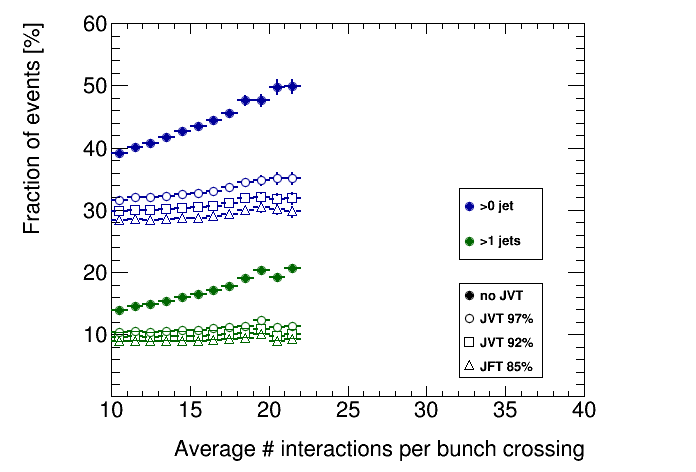
\includegraphics[trim=0.0cm 0cm 0cm 0cm,width=0.47\columnwidth]{FIGURES/Frac_njets_1and2}
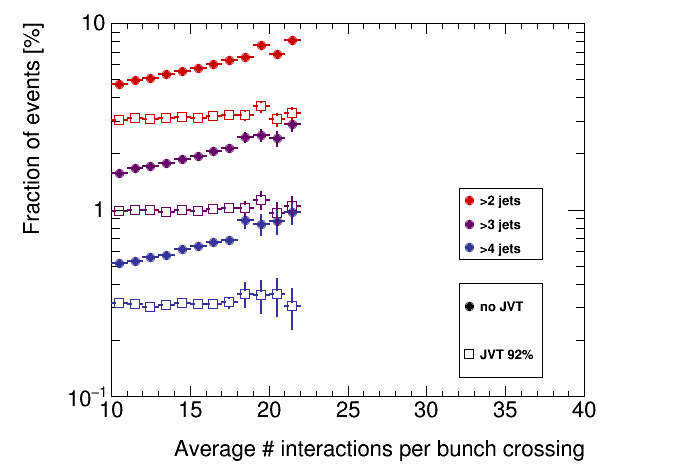
\includegraphics[trim=0.0cm 0cm 0cm 0cm,width=0.47\columnwidth]{FIGURES/Frac_njets_3to5}
\vspace{-0.2cm}
\end{center}
\caption{Fraction of events [\%] in data with at least 1 or 2 jets (left) and with at least 3, 4 or 5 jets (right) with respect to average number of interactions per bunch crossing with and without a cut on the JVT. Event selection requires a pair of leptons, and all jets have \pt~$>$~25\GeV. $L$~=~3.2~fb$^{-1}$ and $\sqrt s$~=~13\TeV.}
\label{Figure:JVF_Dependency_Run2} 
\end{figure}
%%%%%%%%%%%%%%%%%%%%%%%%%%%%%%%%%%%%%%%%%%%%%%%%%%%%%%%%%%%%

\subsubsection{$b$-tagging}

Tagging of $b$-jets is done using the MV2c20 algorithm with the 70\% efficiency 
operating point. This algorithm is based on a neural network using 
the output weights of the JetFitter+IP3D, IP3D and SV1 algorithms as input.
This efficiency working point was favored by optimisation studies performed with MC15 simulated signal and background samples as described below.
Figure~\ref{fig:btagging} shows the $b$-jet multiplicity for the three tagging efficiency working points. 
Monte Carlo background distributions are shown after same-sign lepton pair requirement.

\begin{figure}[htb!!]
\begin{center}
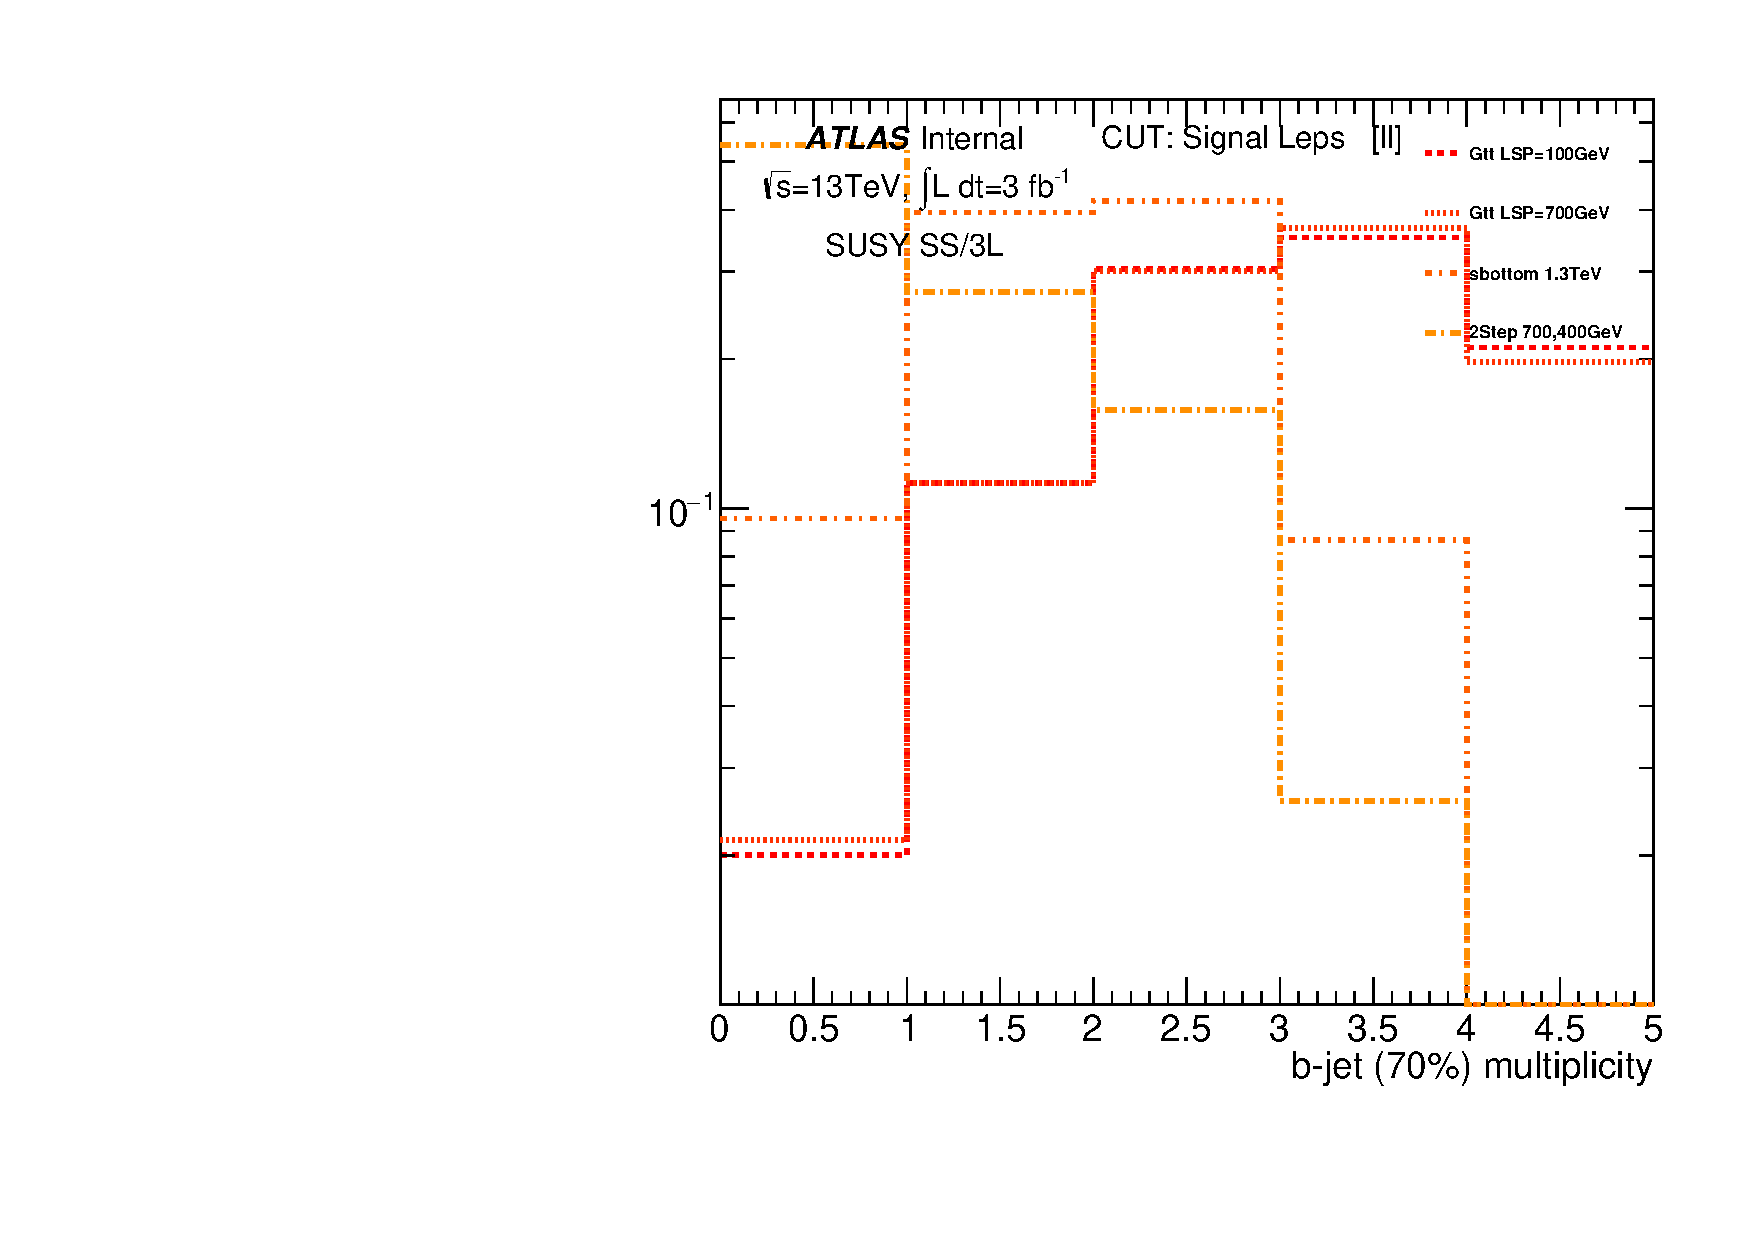
\includegraphics[width=0.3\textwidth]{FIGURES/BTAGGING/02_CutLEP_ll_NB1JET_signals.pdf} 
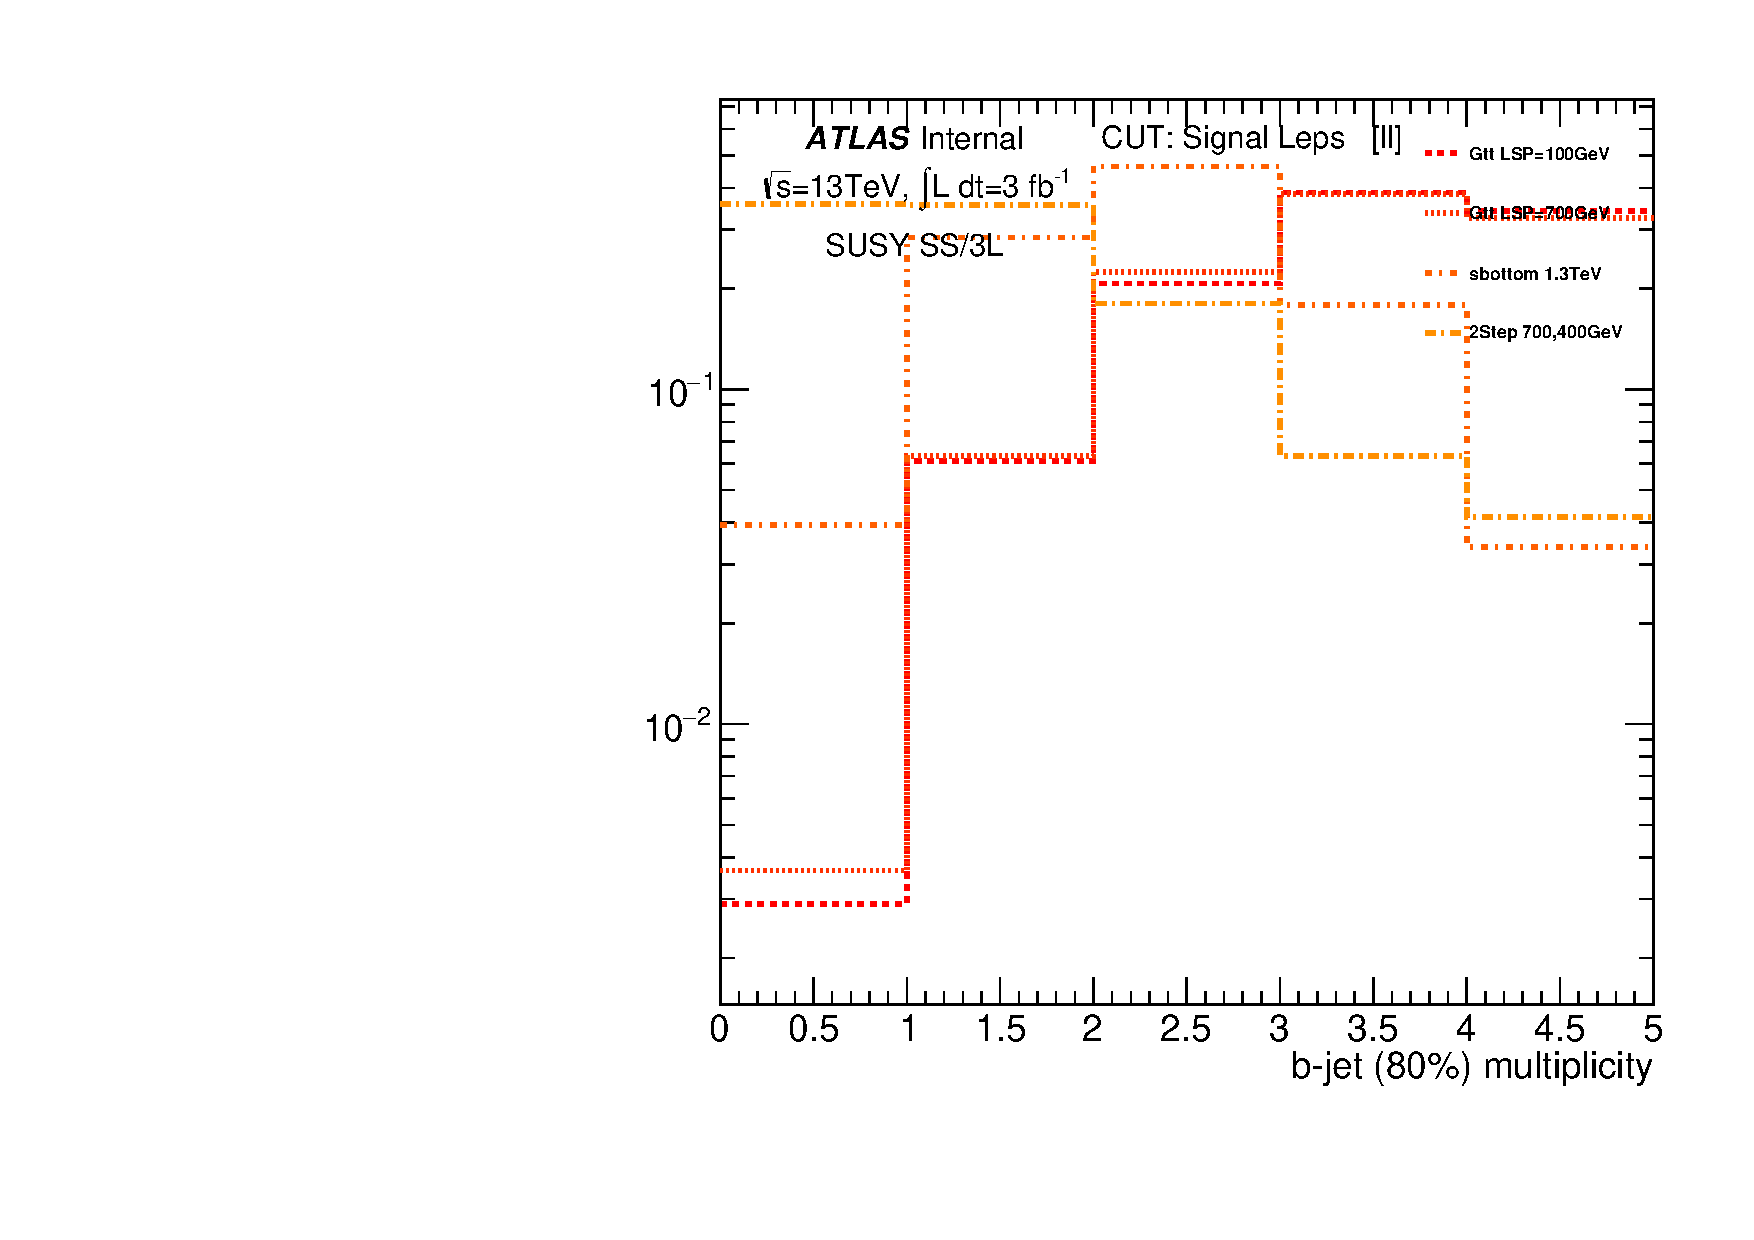
\includegraphics[width=0.3\textwidth]{FIGURES/BTAGGING/02_CutLEP_ll_NB2JET_signals.pdf}
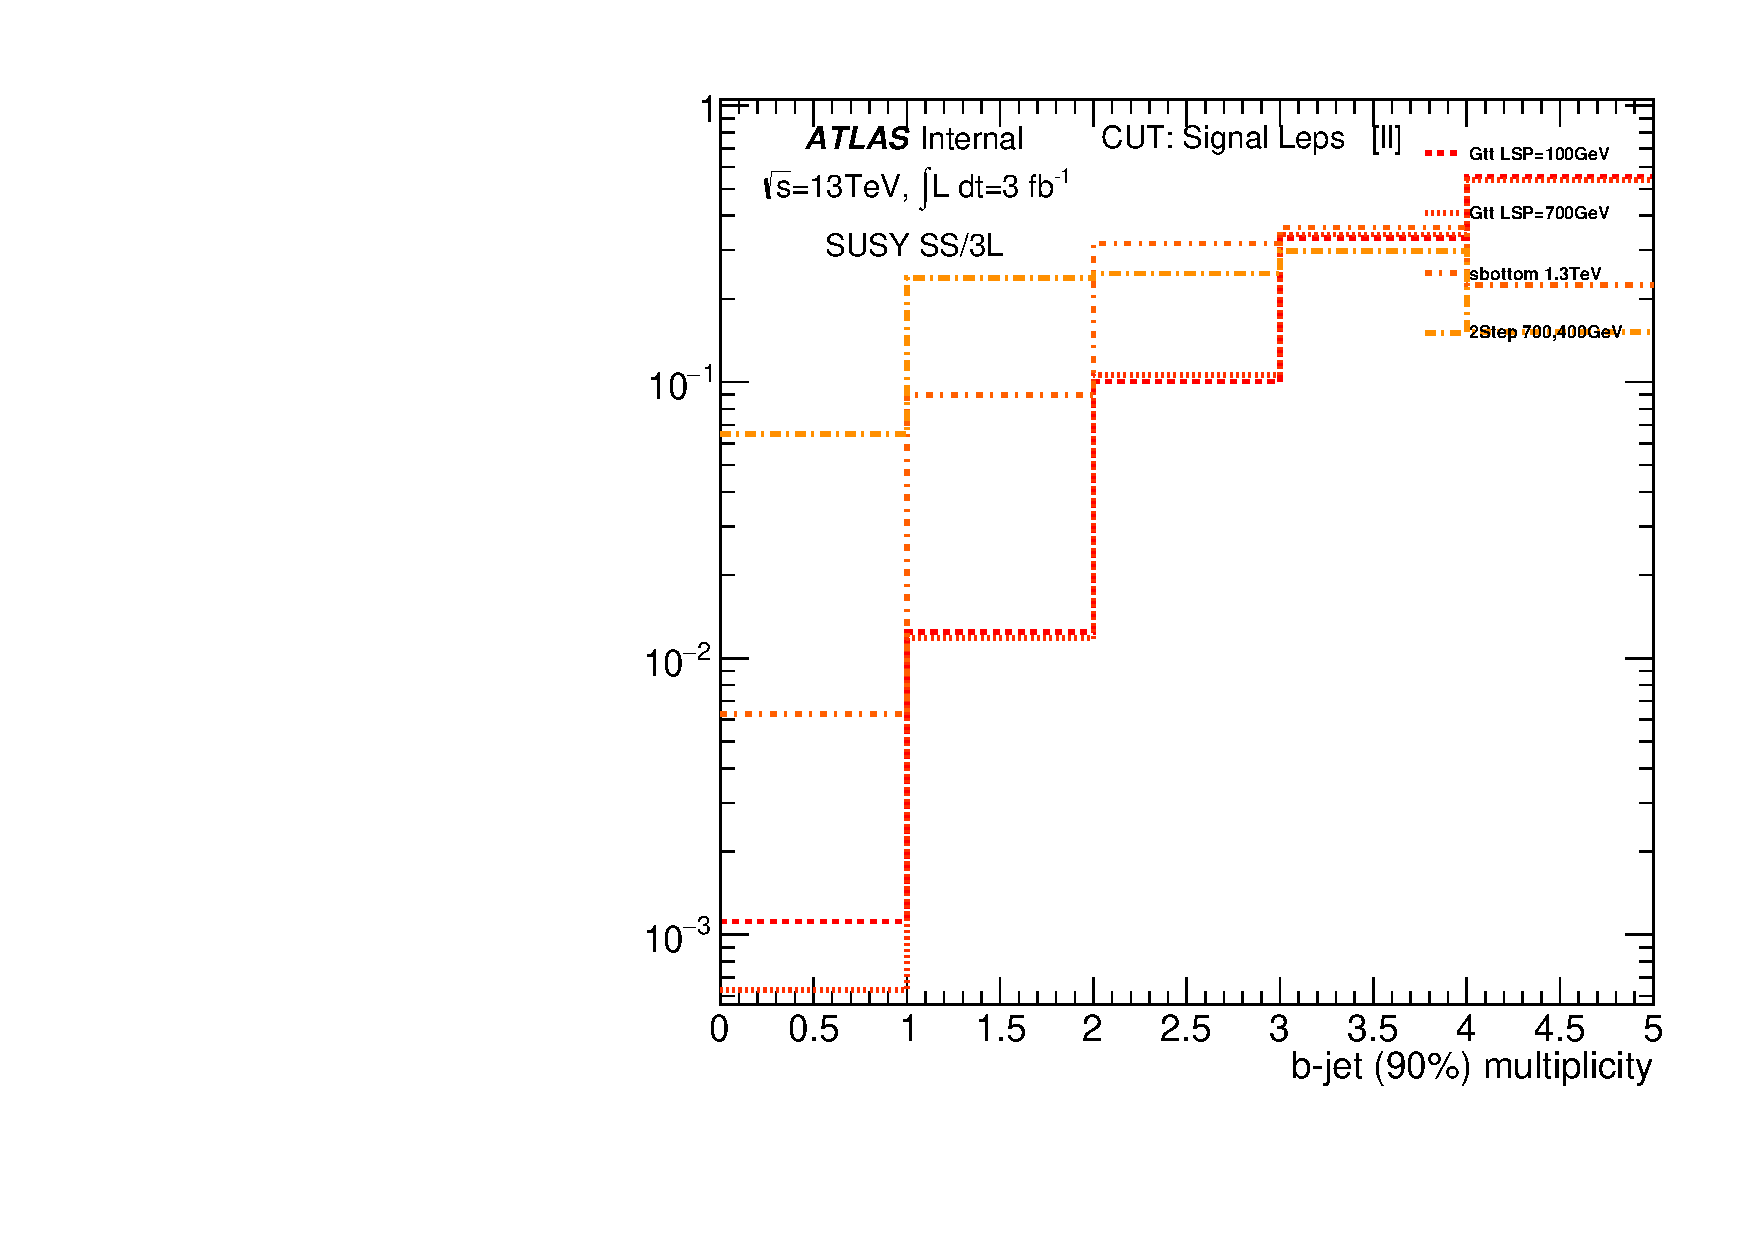
\includegraphics[width=0.3\textwidth]{FIGURES/BTAGGING/02_CutLEP_ll_NB3JET_signals.pdf}\\ 
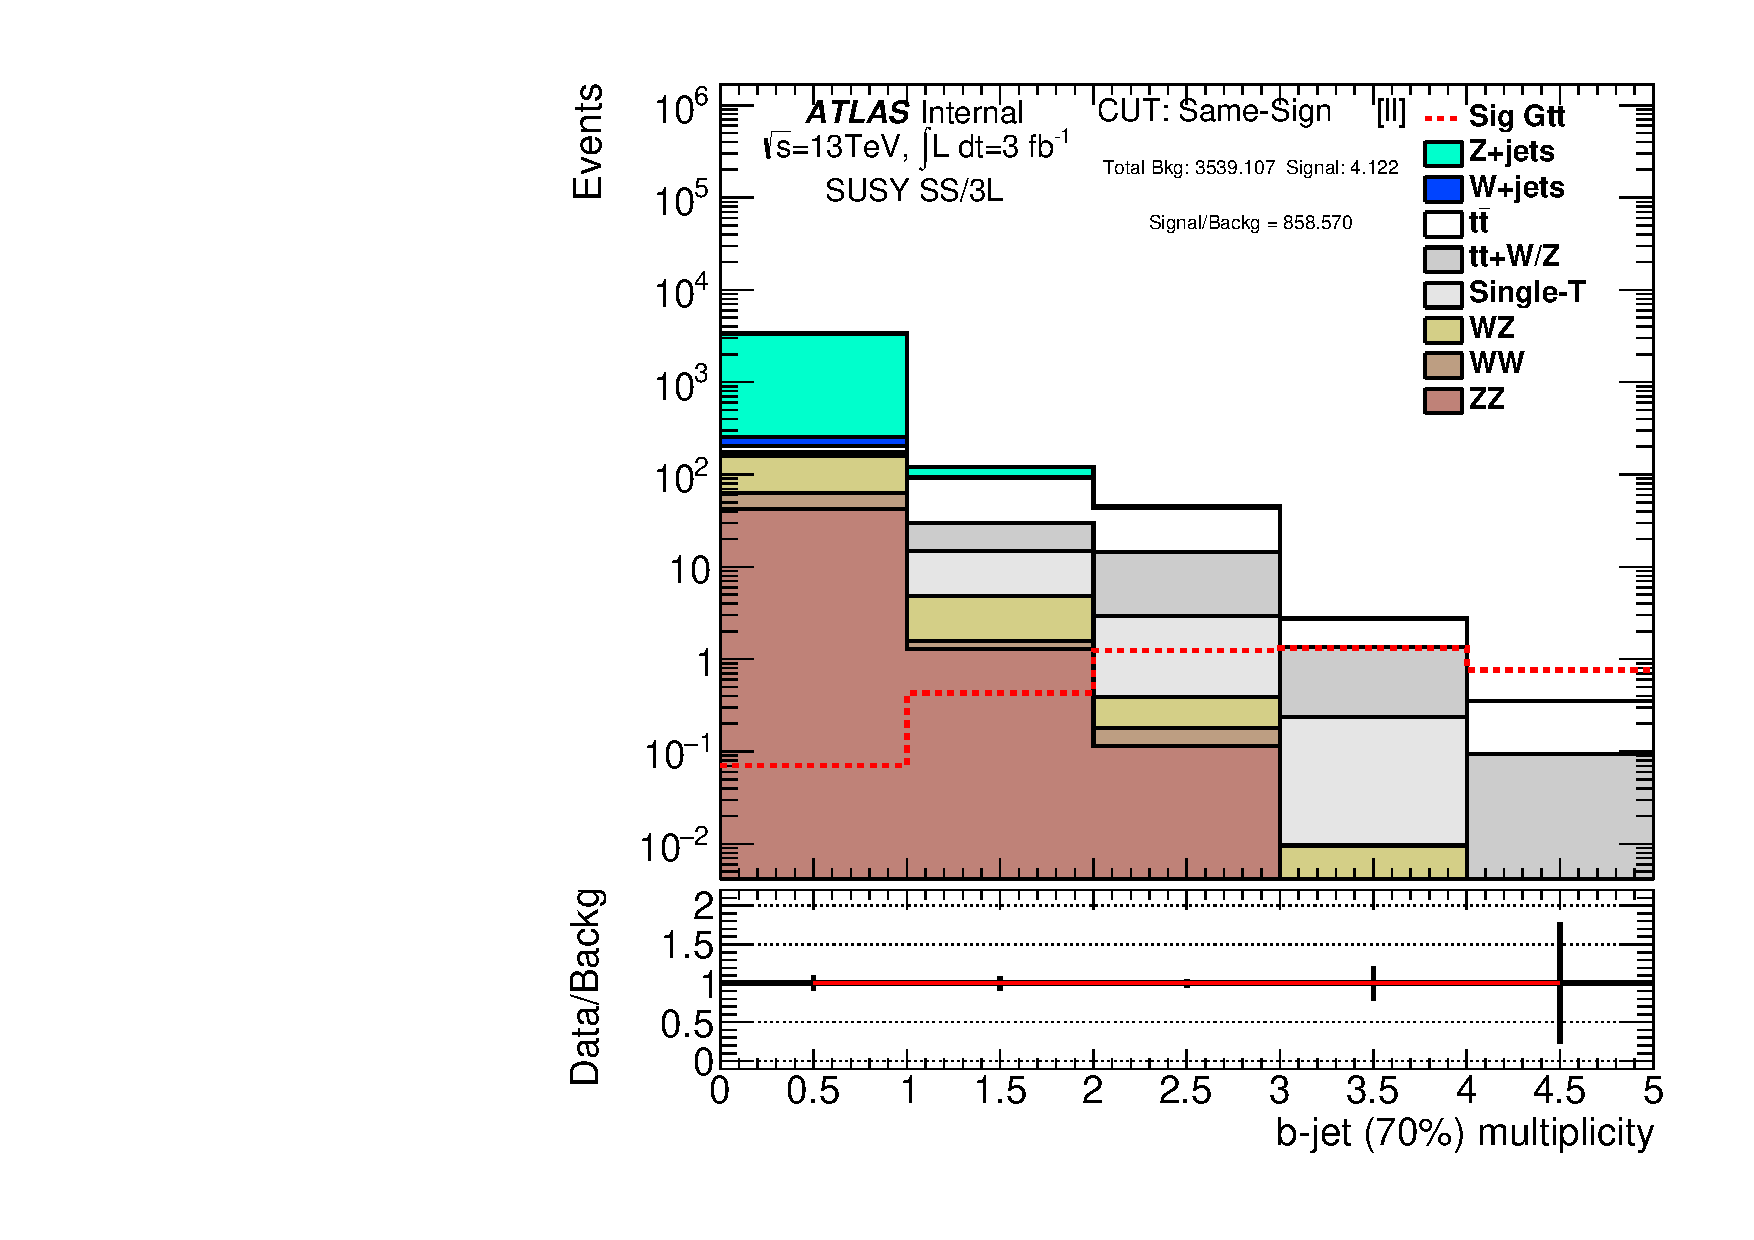
\includegraphics[width=0.3\textwidth]{FIGURES/BTAGGING/05_CutSS_ll_NB1JET.pdf}
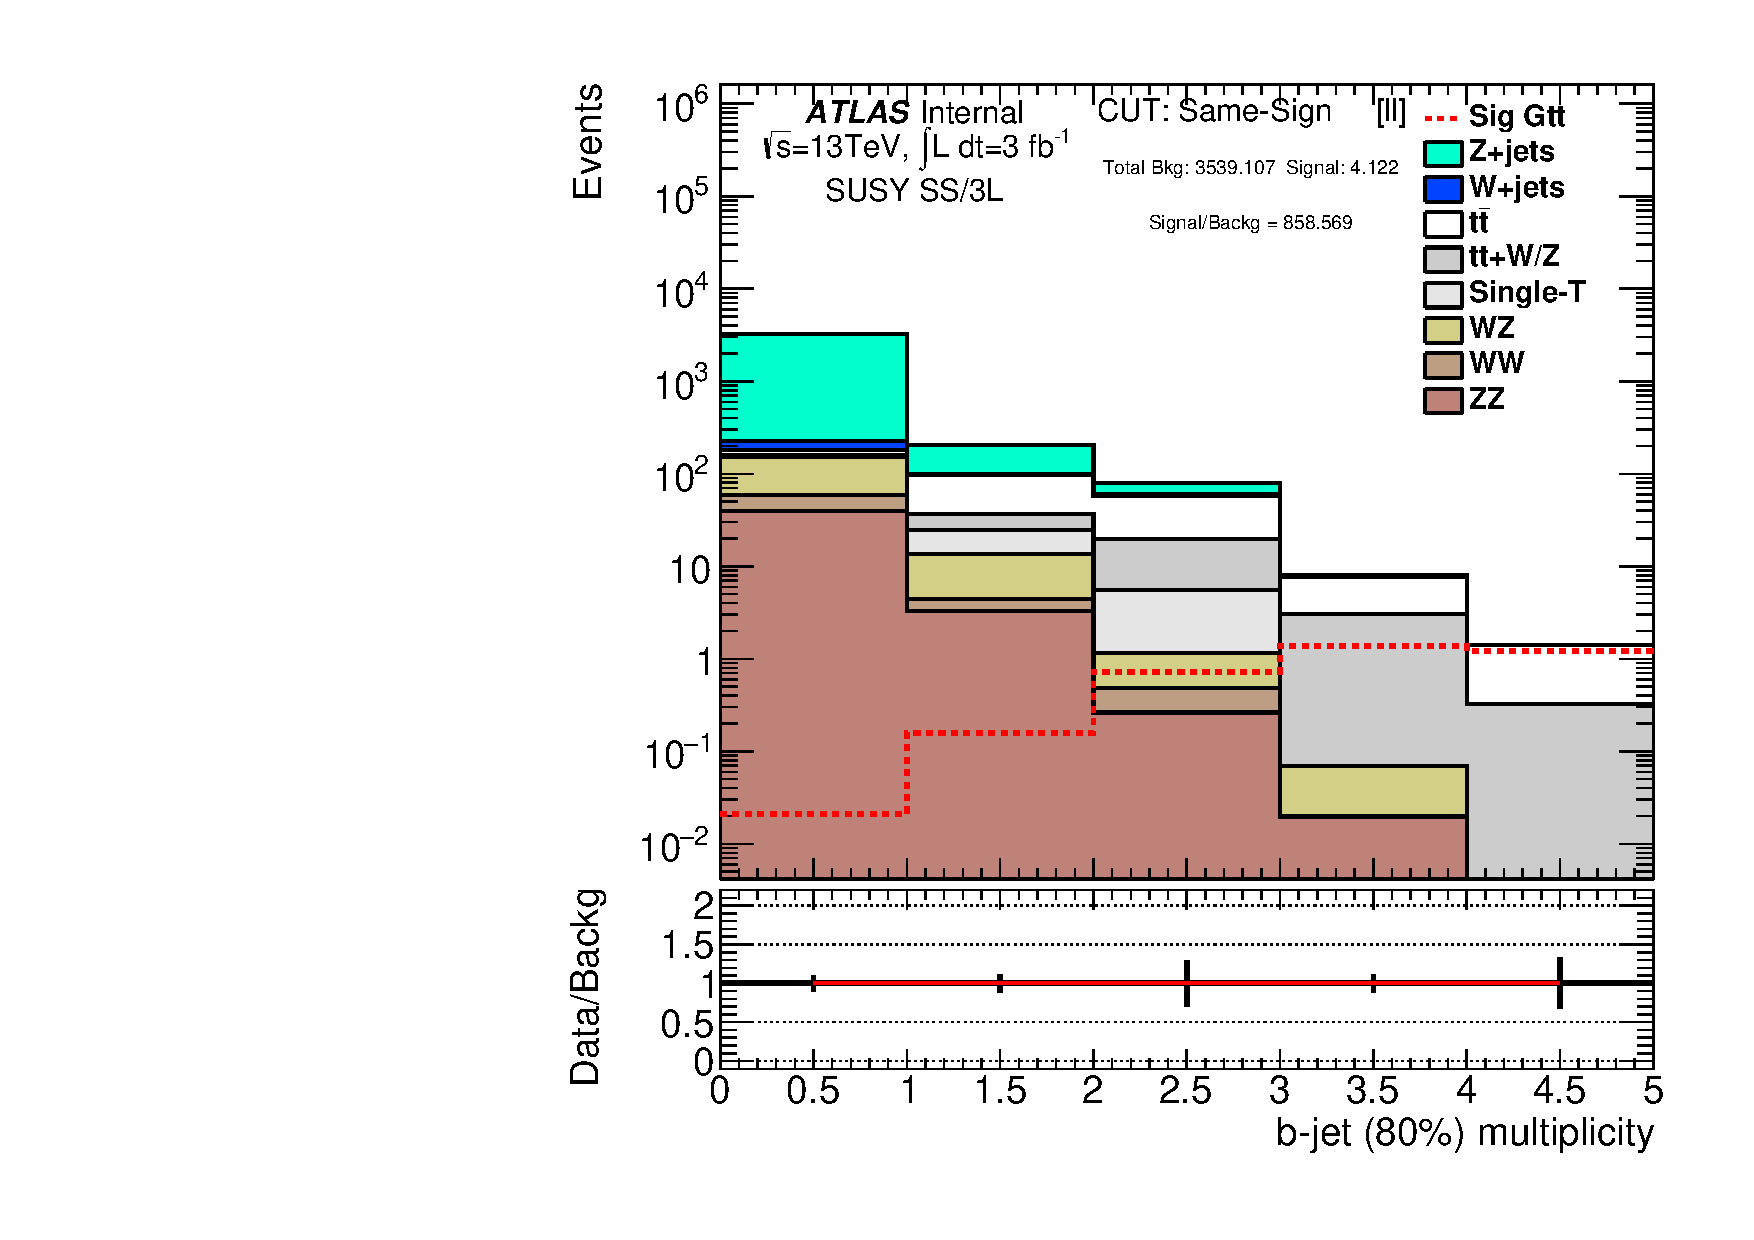
\includegraphics[width=0.3\textwidth]{FIGURES/BTAGGING/05_CutSS_ll_NB2JET.pdf}
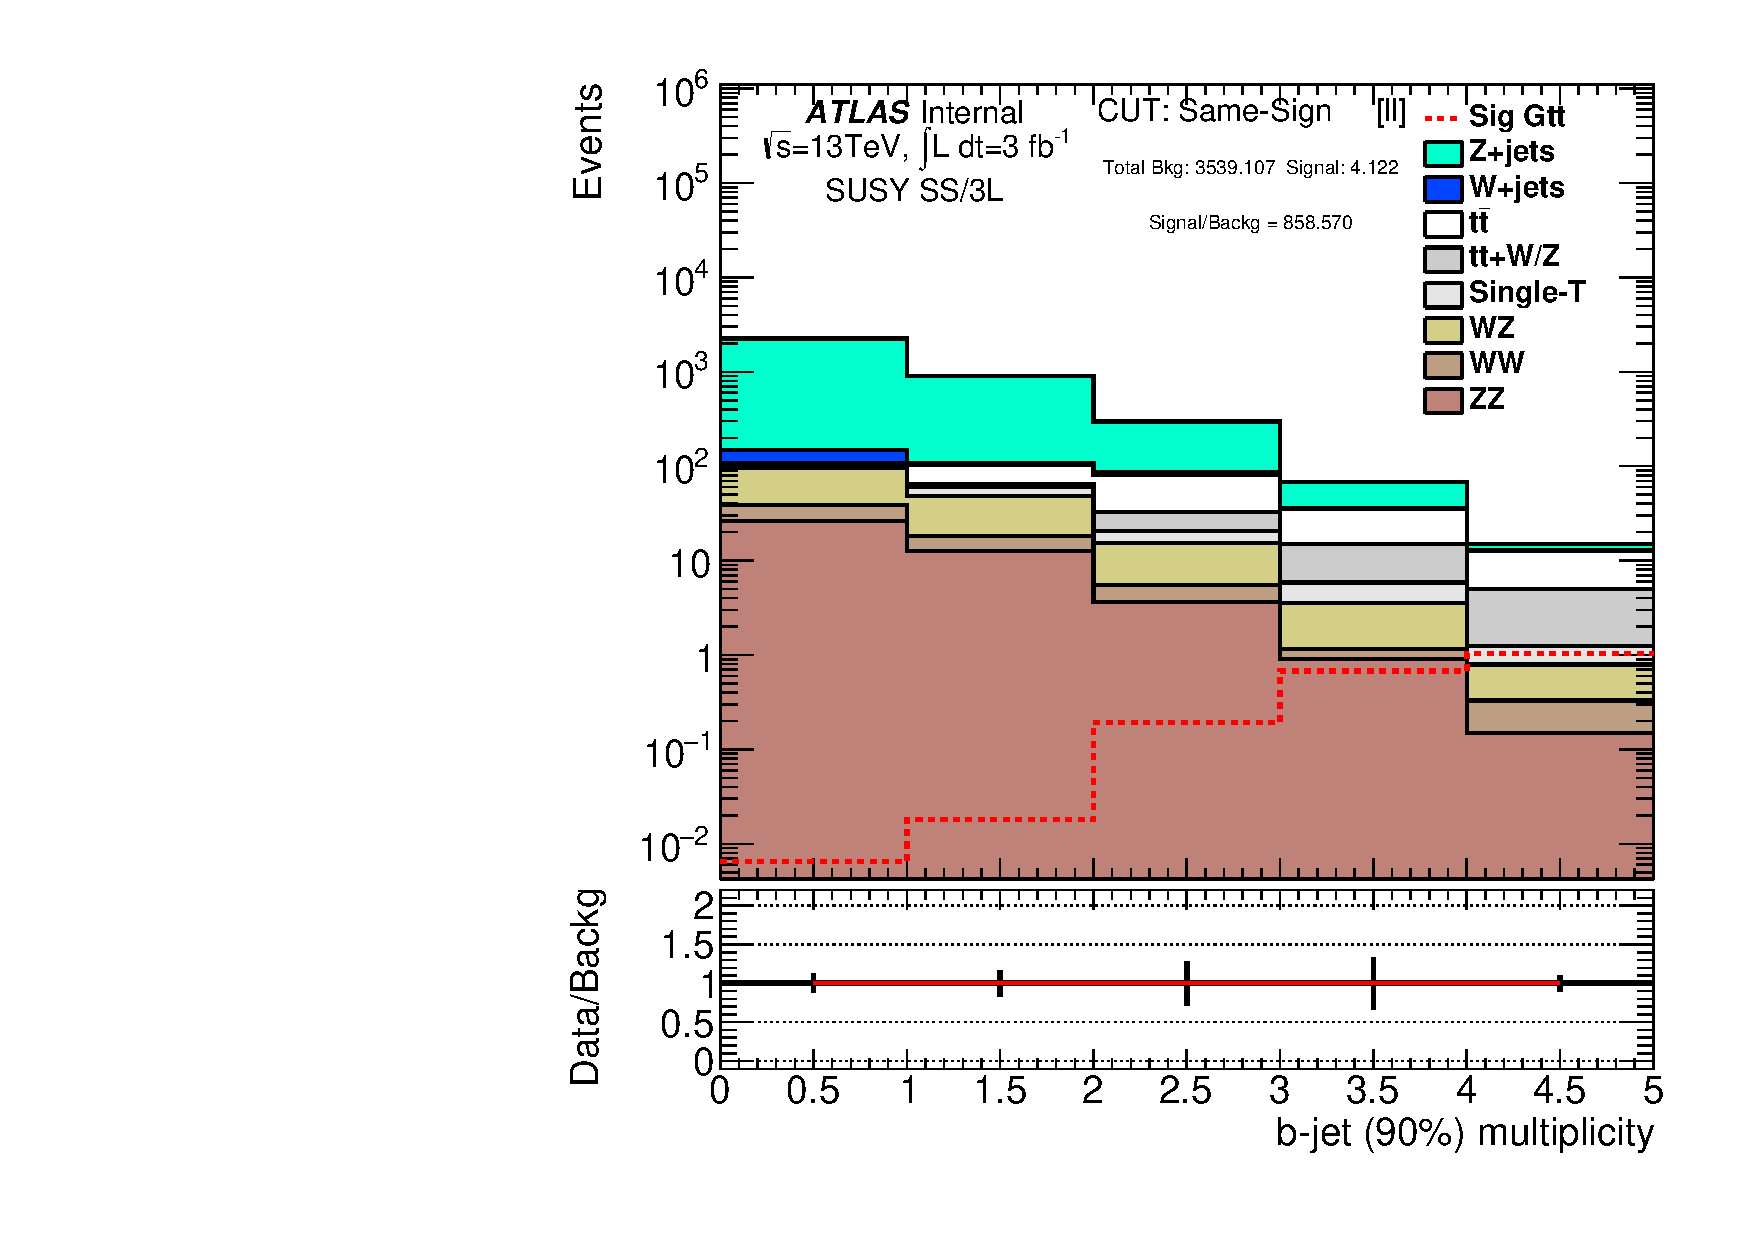
\includegraphics[width=0.3\textwidth]{FIGURES/BTAGGING/05_CutSS_ll_NB3JET.pdf} 
\end{center}
\vspace{-0.2cm}
\caption{$b$-jet multiplicity for three different tagging efficiency working points, left 70\%, center 80\%, right 90\%.
Signals shapes are shown on the top figures, and stacked background expectations for an integrated luminosity of 3~fb$^{-1}$ are shown on the bottom plots.}
\label{fig:btagging}
\end{figure}

Different signal models described earlier on this document are expected to contain different heavy flavour jet multiplicities.
Therefore the choice of the most performant $b$-jet tagging efficiency working point was made by looking into regions that emulate the signal regions that would eventually be used in the analysis.
Table~\ref{tab:btaggingSR} describes the six different signal-like regions used on this optimisation. 

%%%%%%%%%%%%%%%%%%%%%%%%%%%%%%%%%%%%%%%%%%%%%%%%%%%%%%%%%%%%%
\begin{table}[htb!]
\caption{Signal-like region selections used for the $b$-jet efficiency working point optimisation.}
\label{tab:btaggingSR}
\begin{center}
\begin{tabular}{l|c|c|l}
                & \#$\ell$ & \#$b$-jets & Other cuts                          \\ \hline \hline
  SR-3$b$       & $\geq 2$ & $\geq 3$   & $N^{40}_j \geq 6$                    \\
  SR-3$b$ Soft  & $\geq 2$ & $\geq 3$   & $N^{20}_j \geq 7$ \&\& MET$>$150~GeV \\\hline
  SR-1$b$       & $\geq 2$ & $\geq 1$   & $N^{50}_j \geq 4$ \&\& MET$>$150~GeV (!SR3b)\\
  SR-1$b$ Incl  & $\geq 2$ & $\geq 1$   & $N^{40}_j \geq 4$ \&\& MET$>$150~GeV \\\hline
  SR-0$b$- 5j   & $\geq 2$ & $== 0$     & $N^{50}_j \geq 5$ \&\& MET$>$100~GeV \\
  SR-0$b$- 3j   & $\geq 2$ & $== 0$     & $N^{40}_j \geq 3$ \&\& MET$>$200~GeV \\ \hline
\end{tabular}
\end{center}
\end{table}
%%%%%%%%%%%%%%%%%%%%%%%%%%%%%%%%%%%%%%%%%%%%%%%%%%%%%%%%%%%%
         
\begin{figure}[htb!!]
\begin{center}
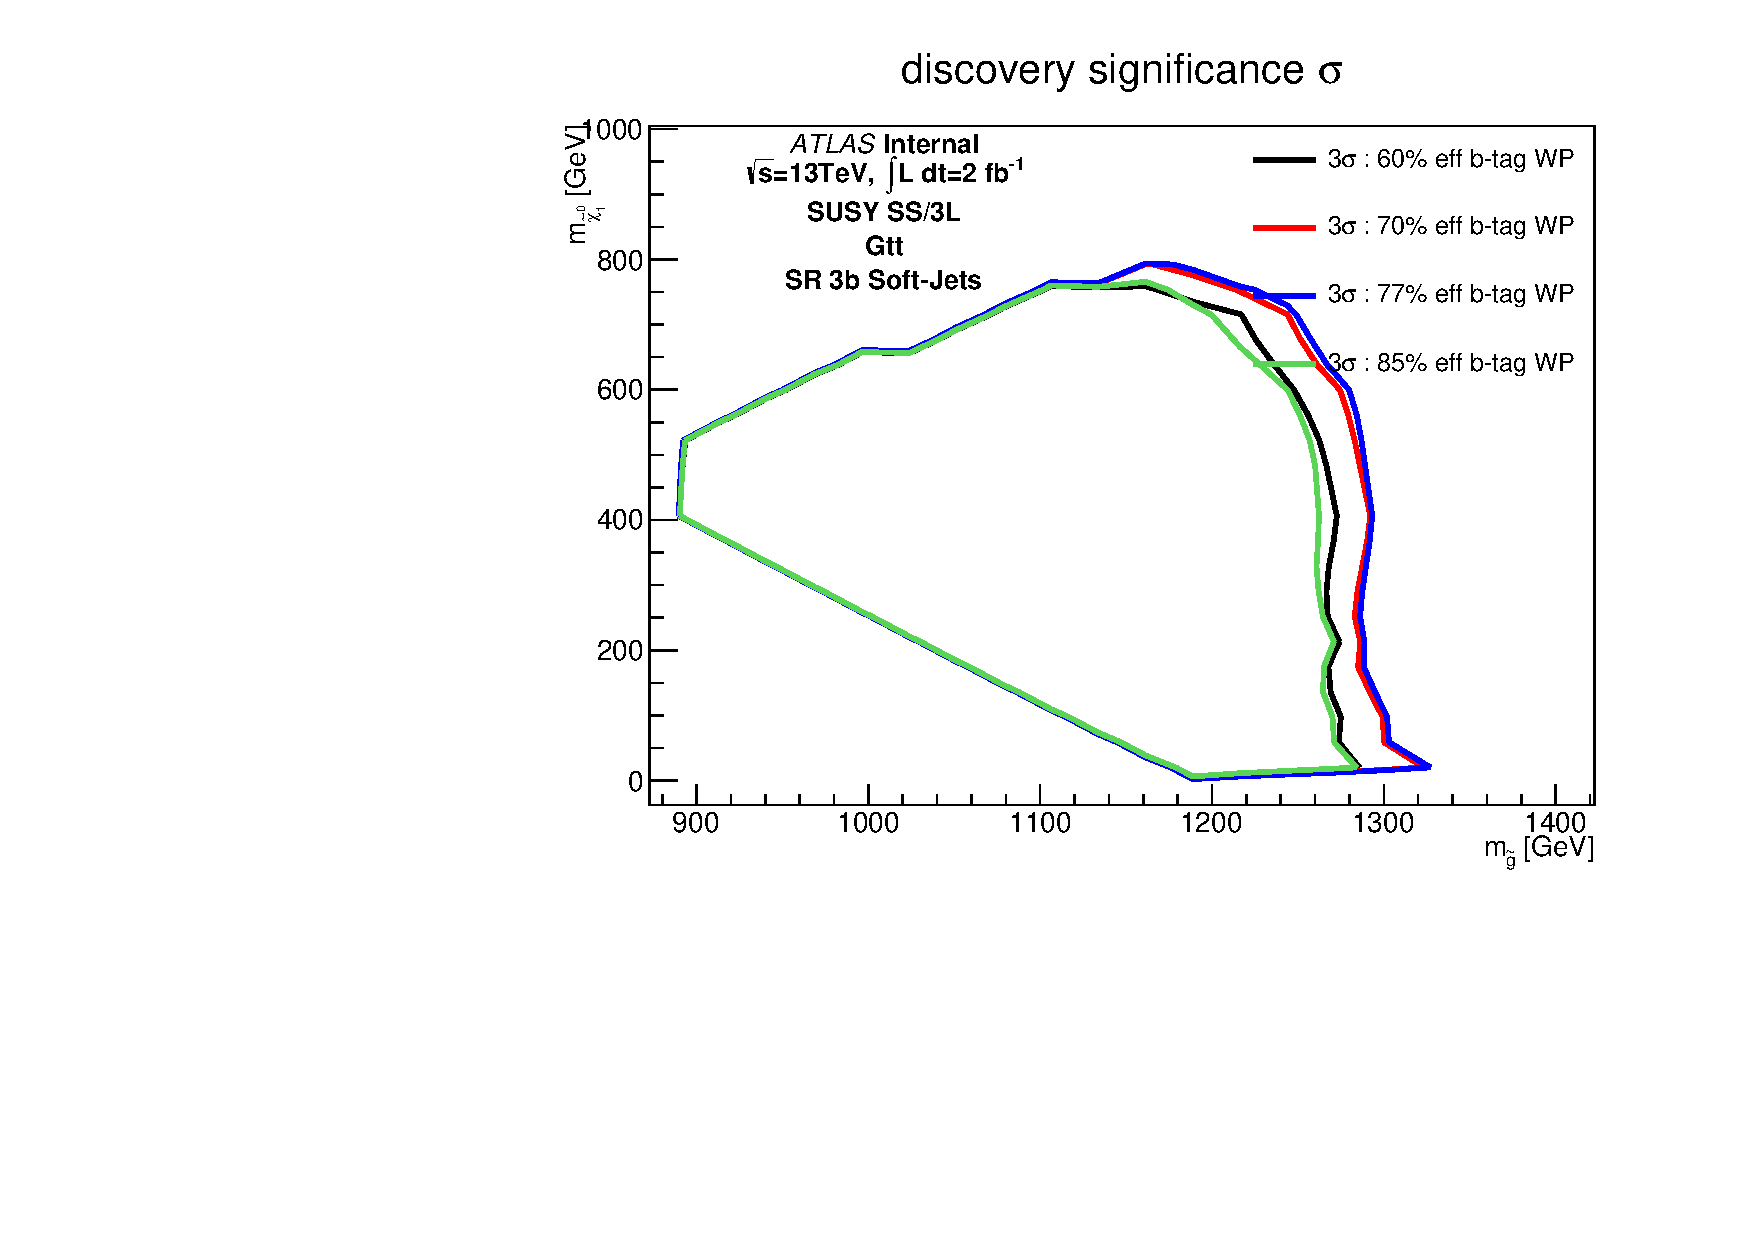
\includegraphics[width=0.45\textwidth]{FIGURES/BTAGGINGMC15/L2fb/plot_significance_gtt_CutSR3BS60_all.pdf}\\
%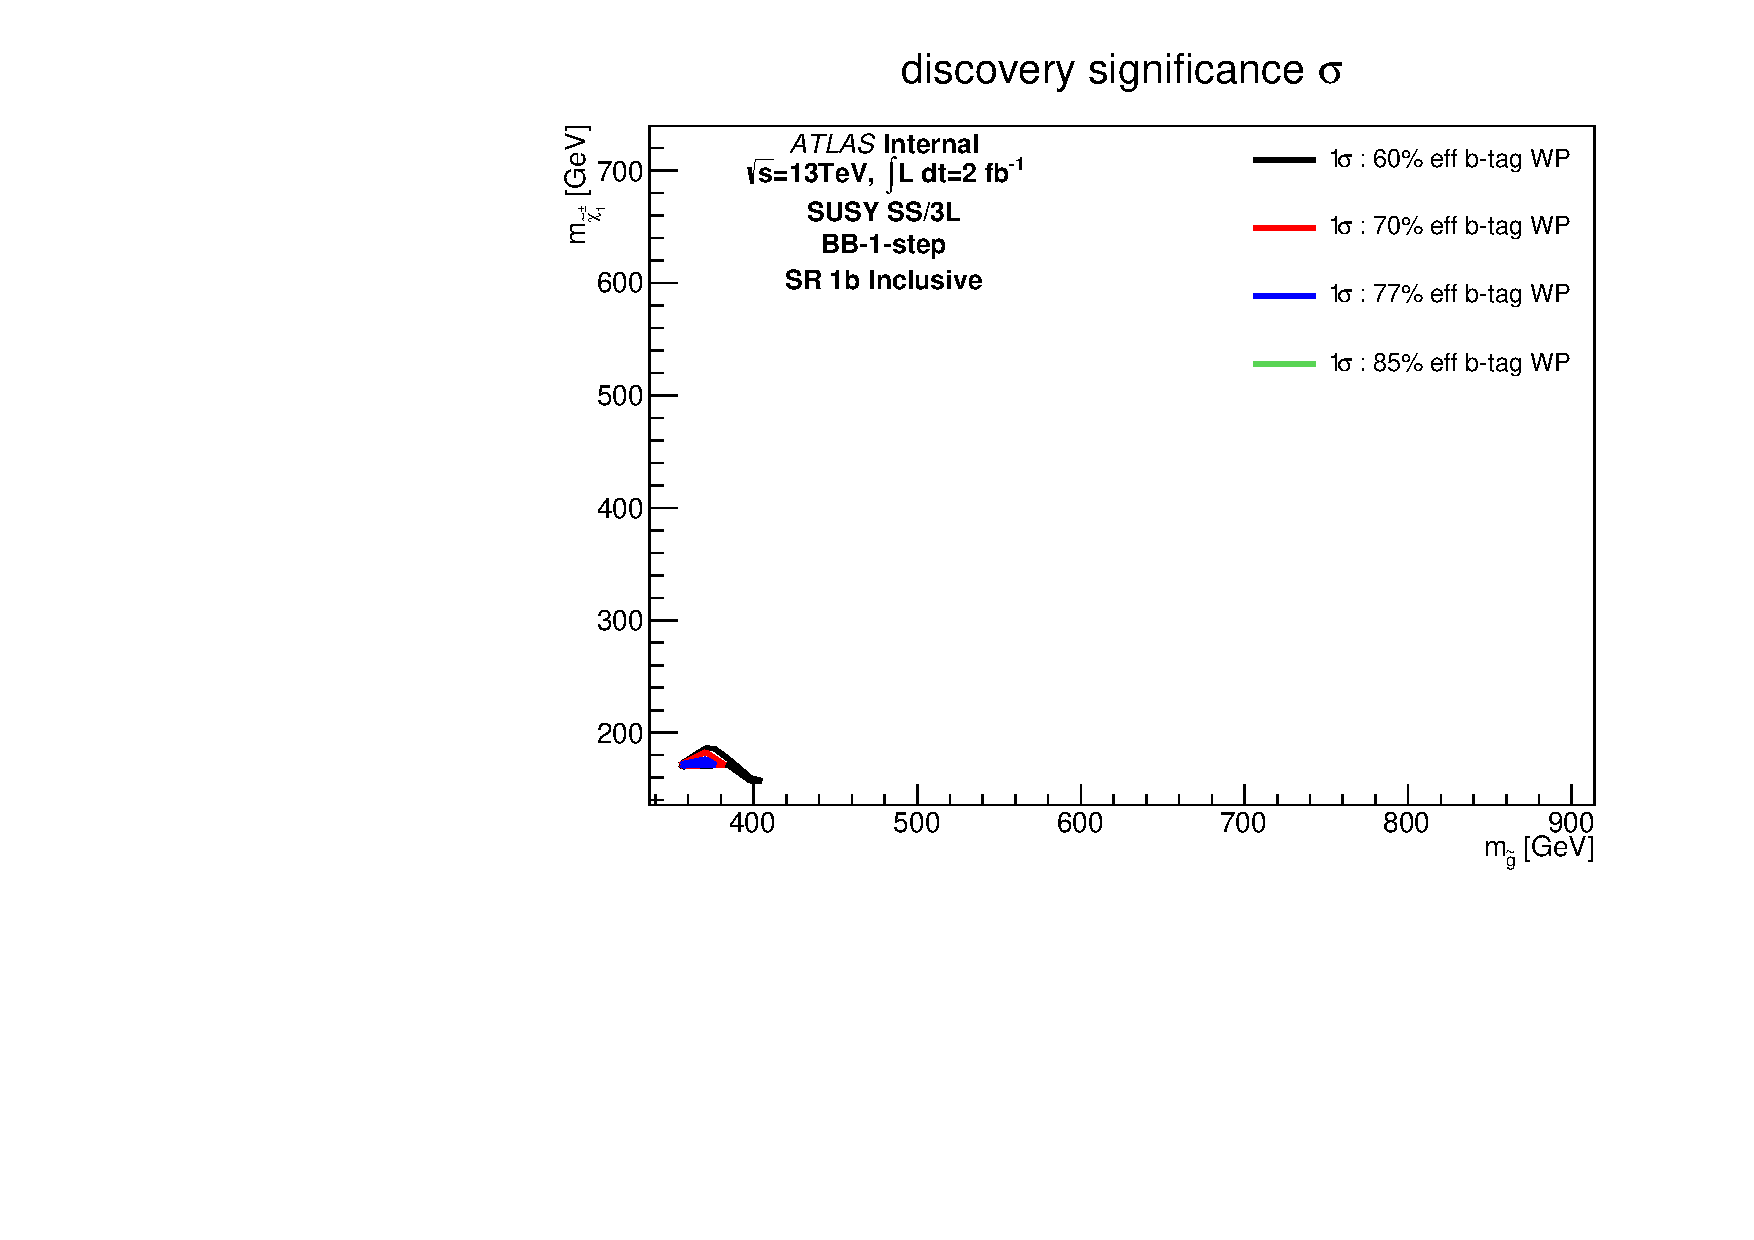
\includegraphics[width=0.3\textwidth]{FIGURES/BTAGGINGMC15/L2fb/plot_significance_bb1step_CutSR1BI60_all.pdf}\\
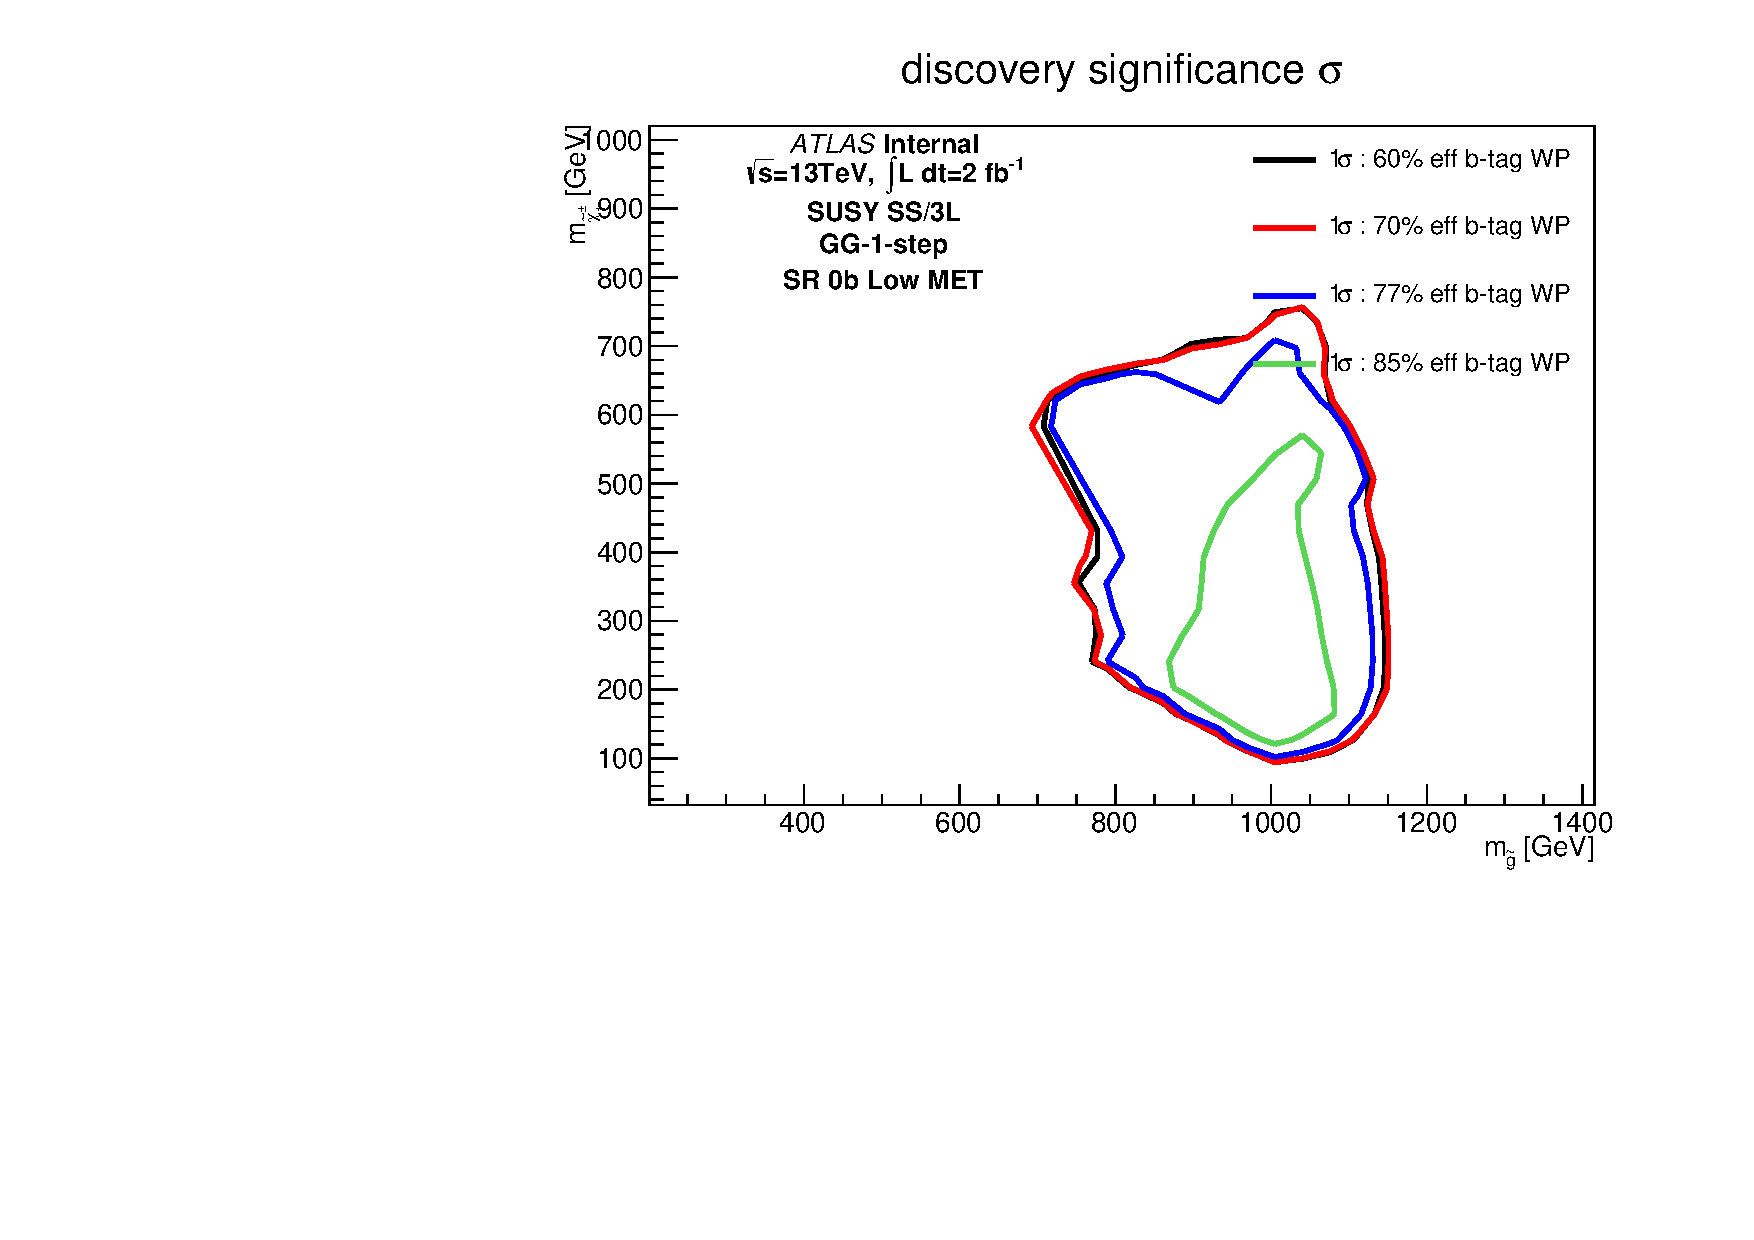
\includegraphics[width=0.45\textwidth]{FIGURES/BTAGGINGMC15/L2fb/plot_significance_gg1step_CutSR0BL60_all.pdf}        
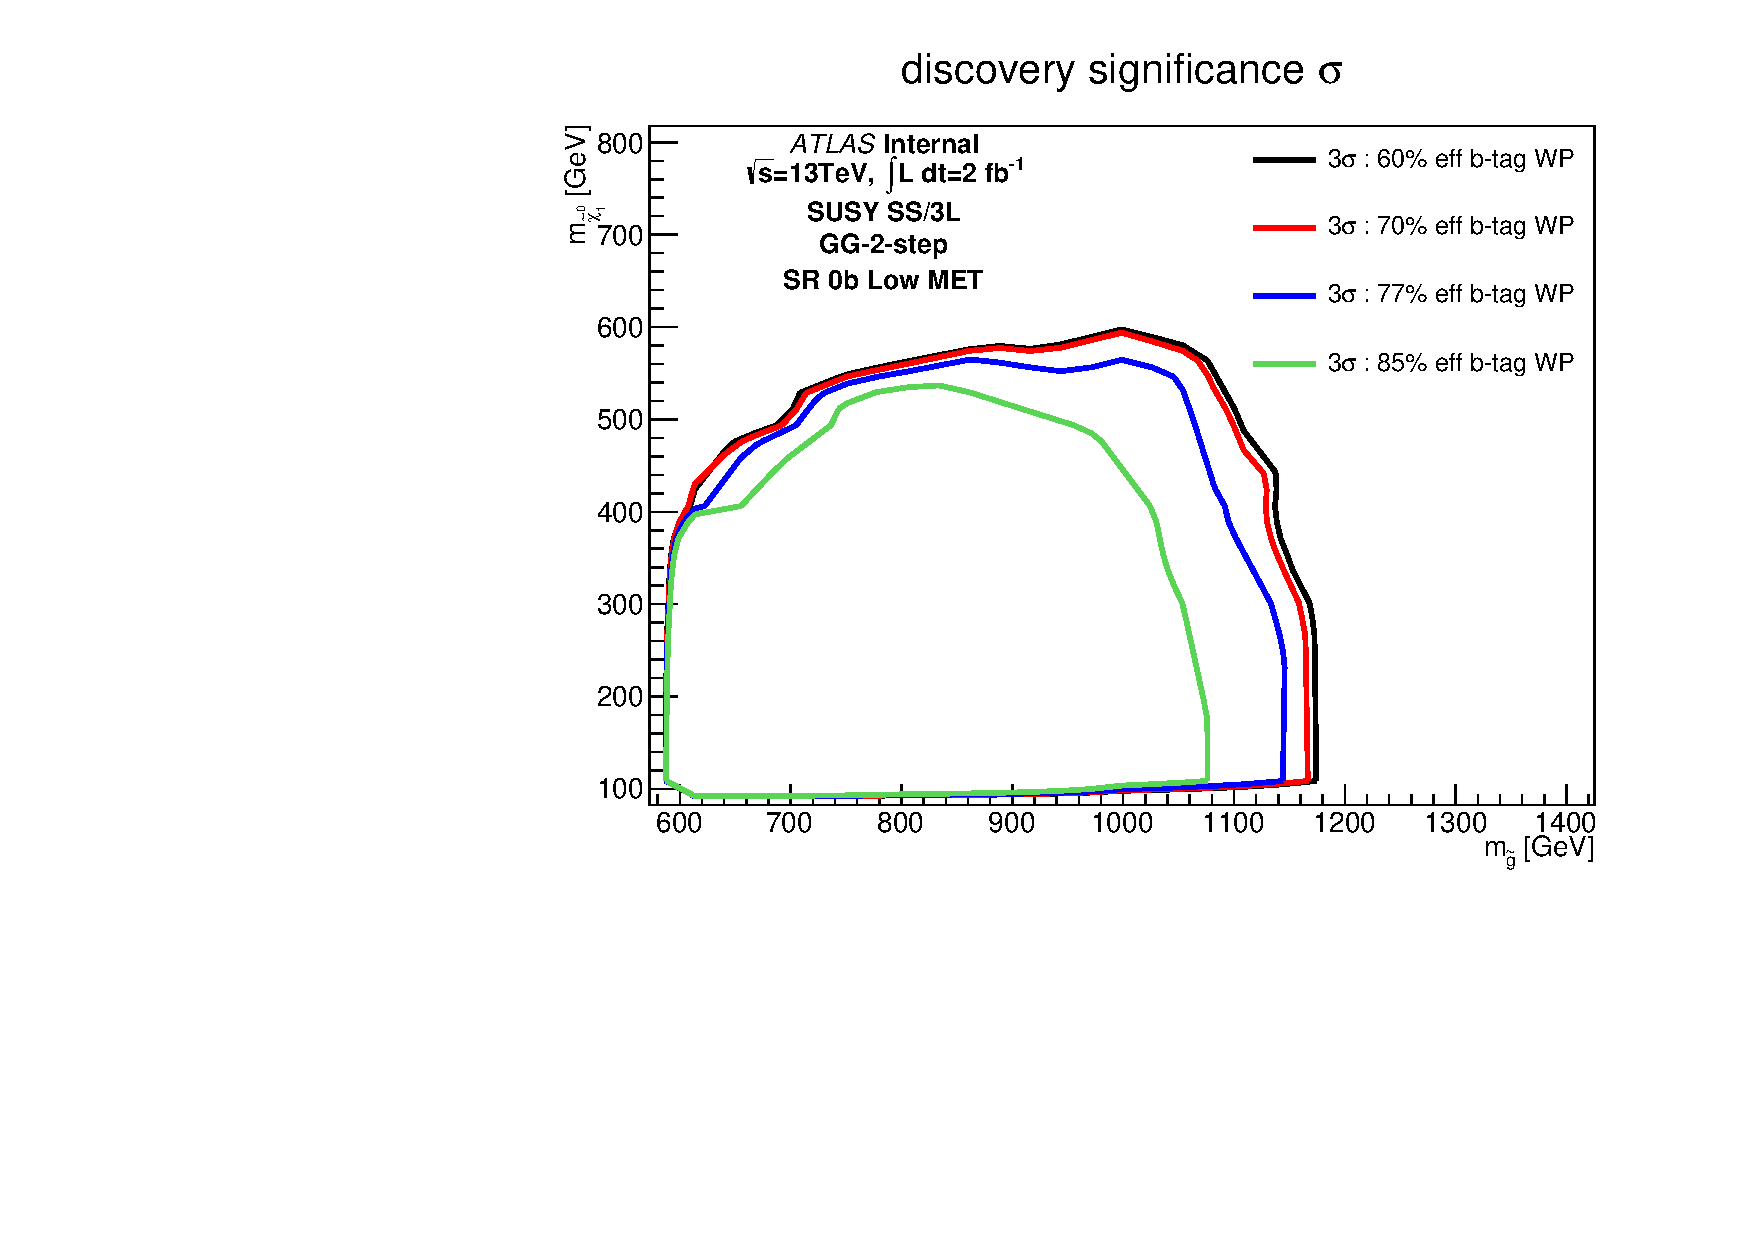
\includegraphics[width=0.45\textwidth]{FIGURES/BTAGGINGMC15/L2fb/plot_significance_gg2step_CutSR0BL60_all.pdf}          
\end{center}
\vspace{-0.2cm}
\caption{Gaussian discovery signal significance for the various signal-like regions where the different models are sensitive.
Three signal models are tested: the gluino-stop off-shell (top), the gluino production mediated by charginos (bottom left) and the 2-step gluinos via charginos (bottom right).
$b$-jet tagging efficiency working points supported by the heavy flavour working group are 60\%(black), 70\%(red), 77\%(blue) and 85\%(green).
Expectations are estimated assuming an integrated luminosity of 2~fb$^{-1}$ of 13~TeV.}
\label{fig:btaggingGrid}
\end{figure}

Figure~\ref{fig:btaggingGrid} shows the discovery signal significance using a simple Gaussian approximation ($S/\sqrt{S+(\Delta B)^2}$) for different choices of the $b$-tagging working point (60\%, 70\%, 77\% and 85\%) with a flat assumption on the background uncertainty of 40\%. The signal region for each of the models was chosen based on the highest sensitivity.
The 3$b$ Soft signal-like region was found to be the most performant for the gluino-stop off-shell production, 
and the 0$b$-5j signal-like region for the gluino production mediated by charginos as well as the 2-step 
gluino production mediated by gauginos. 
%As more signal simulations become available similar studies would be performed for sbottom direct production and gluinos (and squarks) 2-step models mediated via sleptons.
The 70\% $b$-tagging efficiency working point is chosen since it is the best compromise allowing to reach good sensitivity in the different tested signal models.

%Similar studies with detailed information comparing the performance of previous MV1 (rel-19) tagger and MV2c20 (rel-20) are shown in Appendix~\ref{app_btagging}.

\subsection{Leptons}
\label{sec:objects_leptons}

This section summarizes the electron and muon object selection, as well as developments done in the optimization of the
lepton isolation and electron acceptance cuts.

\subsubsection{Electrons}
\label{sec:objects_electrons}

The electron selection is summarized in Table~\ref{tab:lepdef}. The Egamma CP group recommends the likelihood-based electron identification~\cite{ATLAS-CONF-2014-032} for Run-2, since it provides a factor of two better background rejection than the cut-based identification.
Four working points ({\tt VeryLooseLH}, {\tt LooseLH}, {\tt MediumLH}, {\tt TightLH}) are available for LH electrons.

Pre-selected electrons must satisfy the {\tt LooseLH} requirements and have $E_\mathrm{T}>10$~GeV and $|\eta|<2.47$. 
Electrons in the LAr crack region ($1.37<|\eta|<1.52$) are rejected to reduce the contribution from non-prompt electrons. 
A requirement on the transverse impact parameter of $|d_0/\sigma(d_0)|<5$ (as recommended by TrackingCP) is also applied to pre-selected electrons and helps reducing the contribution from charge mis-identification. 
Signal electrons are additionally required to pass the isolation cuts defined in~\ref{sec:isolation} 
as well as the {\tt TightLH} identification criteria and standard requirements of the longitudinal impact parameter ($|z_0 \cdot sin(\theta)|<$ 0.5 mm, as recommended by TrackingCP).

A multiplicative event weight is applied for each signal electron in MC to the overall event weight 
in order to correct for differences in efficiency between data and MC as recommended by the Egamma group.

\subsubsection{Muons}
\label{sec:objects_muons}

The muon selection is summarized in Table~\ref{tab:lepdef}. The Run-2 muon reconstruction is performed by the so-called \textit{third chain}: 
it has been designed to combine the best features of the Run-1 STACO and MUID chains to provide the best performance. 
The following muon selection working points are supported:
{\tt Tight}, {\tt Medium}, {\tt Loose} and {\tt VeryLoose}. 

Pre-selected muon candidates must pass the {\tt Medium} muon quality cuts and have  $p_\mathrm{T} > 10\GeV$ and $|\eta| < 2.4$.
A smearing procedure is applied to the muon $p_\mathrm{T}$.  
A multiplicative event weight is applied for each selected muon in MC to the overall event weight in order to correct for differences in efficiency between data and MC as recommended by the Muon CP group. 

Finally, signal muon candidates are required to pass the isolation cuts defined in~\ref{sec:isolation} as well as the requirements on the impact parameter of $|d_0/\sigma(d_0)|<3$ and $|z_0 \cdot sin(\theta)|<$ 0.5 mm, as recommended by TrackingCP.


Note that events with ``cosmic'' muons, or ``Bad'' muon are vetoed as described in Section~\ref{sec:presel}.


%%%%%%%%%%%%%%%%%%%%%%%%%%%%%%%%%%%%%%%%%%%%%%%%%%%%%%%%%%%%%
\begin{table}[htb!]
\caption{Summary of the electron and muon selection criteria. The signal
  selection requirements are applied on top of the preselection. The
  lepton-jet isolation requirement is applied after electron-jet overlap
  removal.}
\label{tab:lepdef}
\begin{center}
    \begin{tabular}{|l|c|c|}
      \hline
      \hline
       & \textbf{Pre-selected Electron} & \textbf{Pre-selected Muon} \\
      \hline
      \hline
      Acceptance     & $\pt > 10\,\GeV, |\eta^\mathrm{clust}| < 2.47$  & $\pt > 10\,\GeV, |\eta| < 2.5$ \\
                     &  except $1.37<|\eta^\mathrm{clust}|<1.52$       & \\
      \hline
      Quality & {\tt LooseLLH} & {\tt{xAOD::Muon::Medium}} \\
%      \hline
%      Impact parameter &  $|d_0/\sigma(d_0)|<$ 5.0 & - \\
      \hline
      $\ell$-jet Isolation      & $\Delta{}R(e,jet)$~$>$~0.4 & $\Delta{}R(\mu,jet)$~$>$~0.4 \\
      \hline
      Impact parameter & $|d_0/\sigma(d_0)|<5.0$  & \\
      \hline\hline
       & \textbf{Signal Electron} & \textbf{Signal Muon} \\
      \hline
      \hline
      Quality & {\tt TightLLH} & -\\
       & $|\eta|<2.0$  & -\\
            \hline
      Isolation                & ``FixedCutTight '' & ``FixedCutTightTrackOnly'' \\
      \hline
      Impact parameter & $|z_0 \cdot sin(\theta)|<$ 0.5 mm   & $|z_0 \cdot sin(\theta)|<$ 0.5 mm \\ 
                       &                                     & $|d_0/\sigma(d_0)| < 3.0$\\
     \hline
\end{tabular}
\end{center}
\end{table}
%%%%%%%%%%%%%%%%%%%%%%%%%%%%%%%%%%%%%%%%%%%%%%%%%%%%%%%%%%%%


\subsubsection{Lepton isolation}
\label{sec:isolation}

The isolation working points proposed from this analysis were accepted by the ATLAS Isolation forum and implemented as officially supported working points in the {\tt IsolationSelectionTool}. Unless otherwise stated, the following isolation working points are used in the analysis:
\begin{itemize}
\item Electrons: {\tt TightLLH}, ptvarcone20/\pt$<$0.06 and topoetcone20/\pt$<$0.06 (``FixedCutTight'')
\item Muons: ptvarcone30/\pt\ $<0.06$ (``FixedCutTightTrackOnly'')
\end{itemize}
%Note that no isolation scale factors are used so far in the analysis, but will be released by the EGamma and Muon combined performance groups with the whole 2015 dataset.
Isolation scale factors determined by the CP groups for these working points are applied. 

More details on the isolation studies performed in the context of this analysis can be found in Appendix~\ref{app:iso}.



\subsubsection{Electron acceptance}
\label{sec:eleAcceptance}

Dedicated studies have been conducted to evaluate the impact of a reduction of the $|\eta|$ coverage for electrons. 
This is motivated by the fact that the largest contributions from charge-flip and fake lepton backgrounds 
are observed at $|\eta|>2$ and in the LAr crack region ($1.37<|\eta|<1.52$), 
due to poorer detector resolution or increased amount of material in these regions. 

Table~\ref{tab:eleEta} shows the impact on the expected event yields when reducing the electron $|\eta|$ acceptance 
for the two leading electrons (taking a reference the case of $|\eta|<2.3$). The event selection applied to compute those numbers 
requires SS/3L, at least 3 jets with $\pt > 30$~GeV and $m_{ee}$ outside the 84-98~GeV range to reduce the contribution 
from charge flips. 

%%%%%%%%%%%%%%%%%%%%%%%%%%%%%%%%%%%%%%%%%%%%%%%%%%%%%%%%%%%%%
\begin{table}[htb]
\caption{Relative decrease in the event yield when reducing the $|\eta|$ acceptance for the two leading electrons with respect to $|\eta|<2.3$. The reference is considered to be $|\eta|$~$<$~2.47, and the crack region is excluded in all the cases. Numbers are shown for the event selection described in the text and separately for events with 1 or more $b$-jets.}
\label{tab:eleEta}
\begin{center}
    \begin{tabular}{|l|c|c|c|c|c|} \hline
                   & Prompt SS & $\ttbar +W$ & Gtt (G900\_L100) & Non-prompt leptons & Charge flip \\ \hline\hline
==1$b$, $|\eta|<1.37$ & 14\% & 16\% & 12\%  & 28\% & 69\% \\
==1$b$, $|\eta|<2.0$  & 5.4\%  & 6\%  & 7\%&  11\% & 37\% \\ 
==1$b$, $|\eta|<2.3$  & 0.4\%  & 1.5\%  & 4.7\%&  3.6\% &  11\% \\ \hline
$>$1$b$, $|\eta|<1.37$ & 13\% & 18\% & 10\%  & 44\% & 66\% \\
$>$1$b$, $|\eta|<2.0$  & 4.3\%  & 6.5\%  & 2.9\%&  21\% &  30\% \\ 
$>$1$b$, $|\eta|<2.3$  & 1.3\%  & 1.5\%  & 0.3\%&  8\% &  5.8\% \\  \hline
\end{tabular}
\end{center}
\end{table}
%%%%%%%%%%%%%%%%%%%%%%%%%%%%%%%%%%%%%%%%%%%%%%%%%%%%%%%%%%%%

As shown, reducing the acceptance to $|\eta|<2.0$ would reduce the contribution from processes with prompt 
SS/3L by 6.5\% or less, but the reduction in non-prompt leptons (11-21\%) and charge flip (30-37\%) is quite larger. 
Reducing the acceptance more severely for the two leading electrons to $|\eta|<1.37$ would reduce the non-prompt and 
charge flip components by 28-44\% and $\sim$69\%, respectively, with a reduction of only 13-18\% for prompt SS/3L processes. 

Therefore, this study proves that additional rejection against some of the main backgrounds affecting the analysis can be achieved 
by reducing the $|\eta|$ acceptance of the electrons. 
As illustrated in Table~\ref{tab:lepdef} we chose in conclusion to reject electrons with $|\eta|>2.0$ or in the EM calorimeter cracks ($1.37<|\eta_\text{cluster}|<1.52$). 
Note that these requirements are applied to electrons regardless of the lepton multiplicity of the event.

\subsection{Overlap removal}
\label{sec:objects_overlap_removal}

According to the above definitions, one single final state object may fall in more than one category, being therefore effectively double-counted. 
For example, one isolated electron is typically reconstructed both as an electron and as a jet. A procedure to remove overlaps between final state objects was therefore put in place, and applied on pre-selected objects. 
For this iteration, recommendations from the Harmonization effort~\cite{Harmonization} have been fully adopted. 
%The only exception is the usage a narrower cone for the muon-jet overlap removal (0.2 instead of 0.4).
%A gain of a few \% on signal acceptance and background rejection was observed with respect to the previous overlap-removal definitions, where no $b$-jet information, neither jet-track counting was used.
%The small gain is more evident on the muon channels, with up to 9\% higher acceptance for a Gtt sample, more details can be found in the appendix~\ref{app_overlapremoval} 

The procedure performed is described as follows:

\begin{itemize}

\item First, jets that are angularly close (cone of $\Delta R_y < 0.2$, note the usage of rapidity instead of pseudo-rapidity) 
to a pre-selected (non-isolated) electron are removed from the jet list, 
except if the $b$-tagging weight satisfies the 80\% working point (the electron is then likely coming from a semileptonic $b$-quark decay, so it is removed and the jet is kept). 
%Otherwise both the electron and the jet are kept. 

\item Following this, pre-selected electrons are removed if their distance to the closest jet is $\Delta R_y < 0.4$. 
Then if the $\Delta R_y$ between a jet and a muon is less than 0.4, 
one looks at the number of tracks associated to the jet ({\tt xAOD::JetAttribute::NumTrkPt500}): 
if strictly less than 3 the jet is removed (and the muon is kept),  
otherwise the muon is removed (and the jet is kept).
 
\item If there are an electron and a muon with $\Delta R_y<0.01$, the former is likely to originate from a bremsstrahlung 
of the muon. Such a muon momentum is not measured correctly so that in this case, both the electron
and the muon are removed.

\item Finally, if there are two electrons with $\Delta R_y<0.05$,  the electron with the highest \pT is kept and the other one is discarded.

\end{itemize}

Note that preliminary studies with DC14 data showed a few percent gain in sensitivity if using a narrower cone for the muon-jet overlap removal ($\Delta R_y<0.2$), 
but this was found to introduce features in the muon real and fake efficiency used in the matrix method (see Appendix~\ref{App:RealEfficiency}). 
Therefore, for simplicity and robustness in the analysis, it was decided to used the default value of $\Delta R_y<0.4$. 

%If the distance between two electrons is $\Delta R<0.1$, it is most likely to be that two
%tracks are associated with one calorimeter cluster mistakenly. In this case, lower $E_{\rm T}$ electron 
%is removed. Also 
% OLD TEXT:
%If there are an electron and muon with $\Delta R<0.1$, it is likely to be the bremsstrahlung
%of the muon, and it is therefore removed.

%Studies supporting the update to the latest recommendations (and choice of narrower cone mentioned above) are described below.
%
%Since signal samples in MC15 were not available at the time the study was performed, DC14 samples (signal and background) were used.
%Various signals models were used (Gtt 1300~GeV, $\tilde{\chi_0}$=100~GeV, Gtt 1300~GeV, $\tilde{\chi^0_1}$=700~GeV, sbottom 1300~TeV, 2-step (gluino) 700,400GeV) 
%to obtain significance estimates for different cone-distance used in the overlap-removal between jets and muons.
%Figure~\ref{fig:OR_significance} show the significance (using a Poissonian estimator) for the various flavour channels as well as their combination, after full event selection requirements.
% 
%\begin{figure}[htb!!]
%\begin{center}
%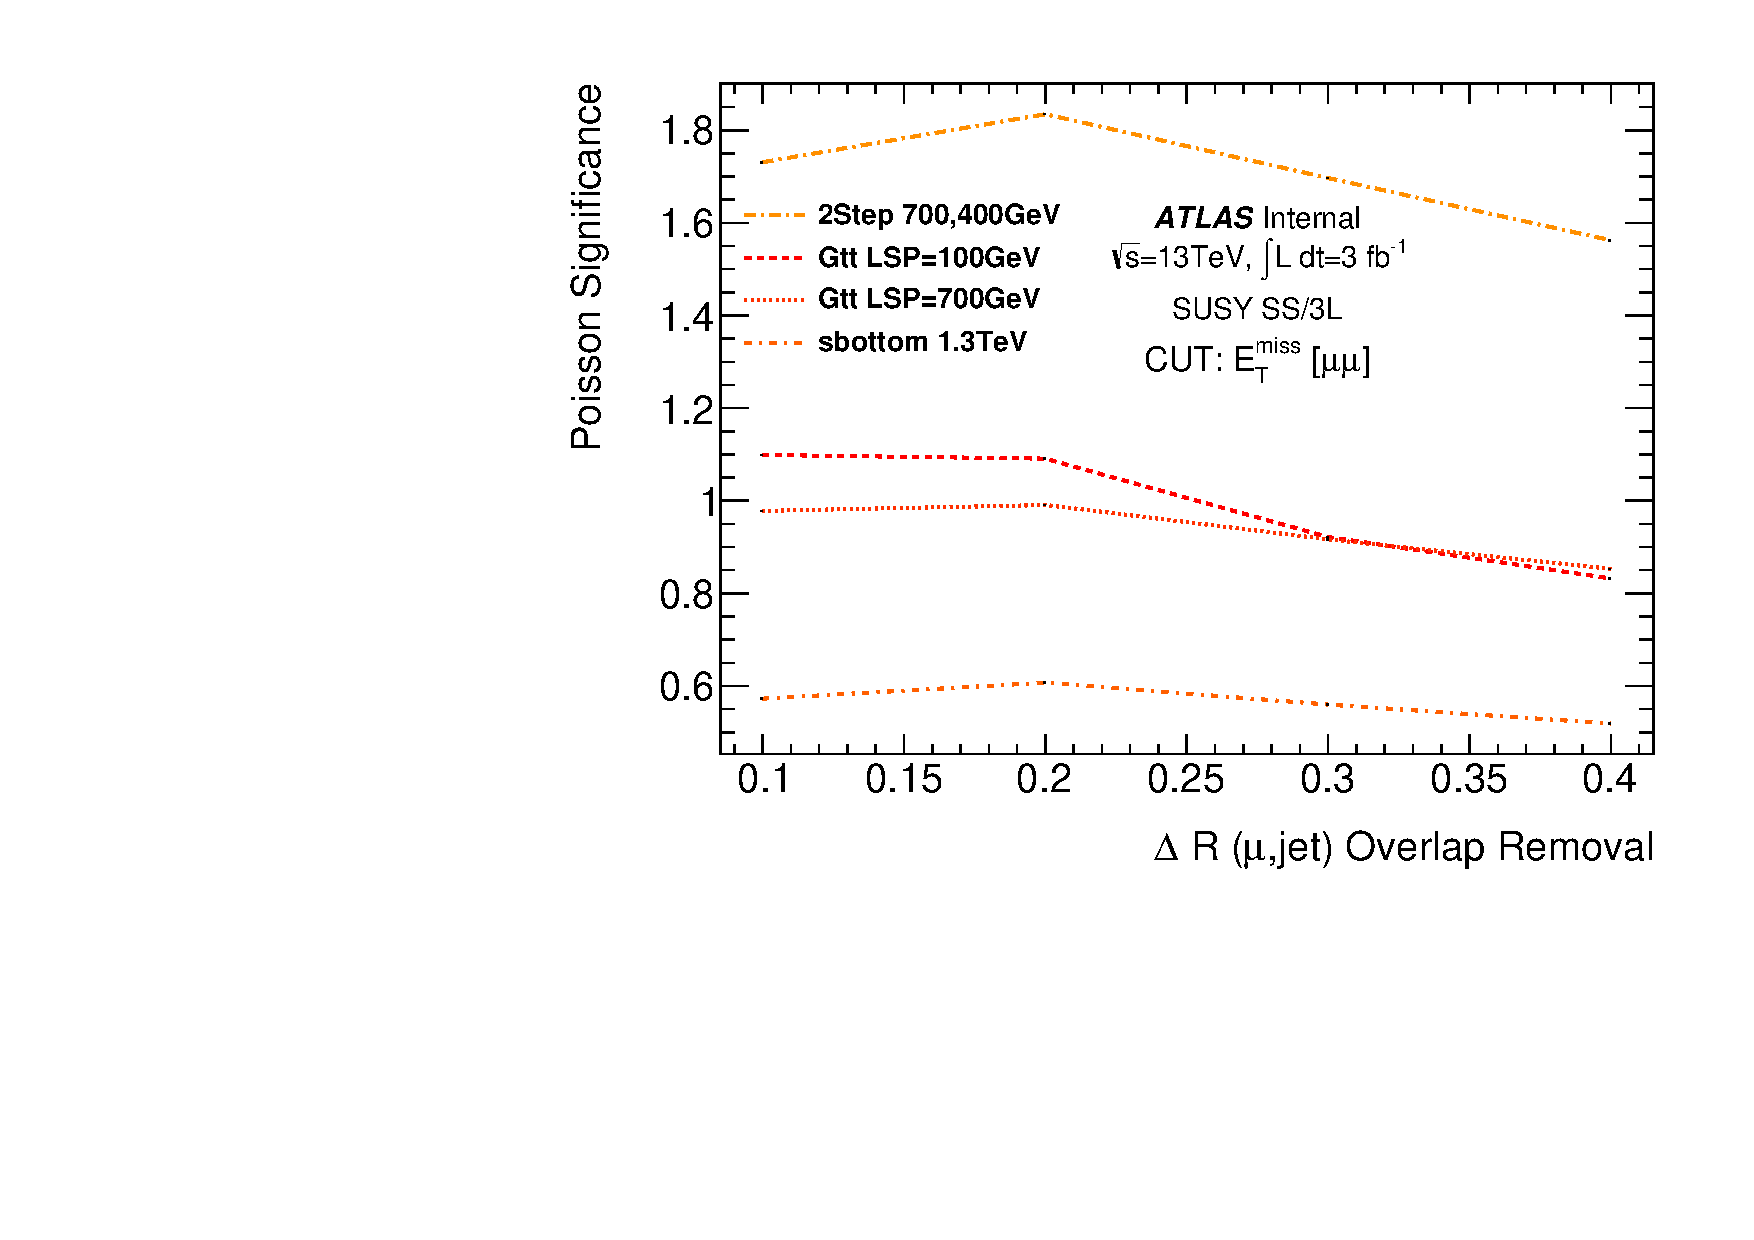
\includegraphics[width=0.45\textwidth]{OVERLAPREMOVAL/plot_significance_mm.pdf} 
%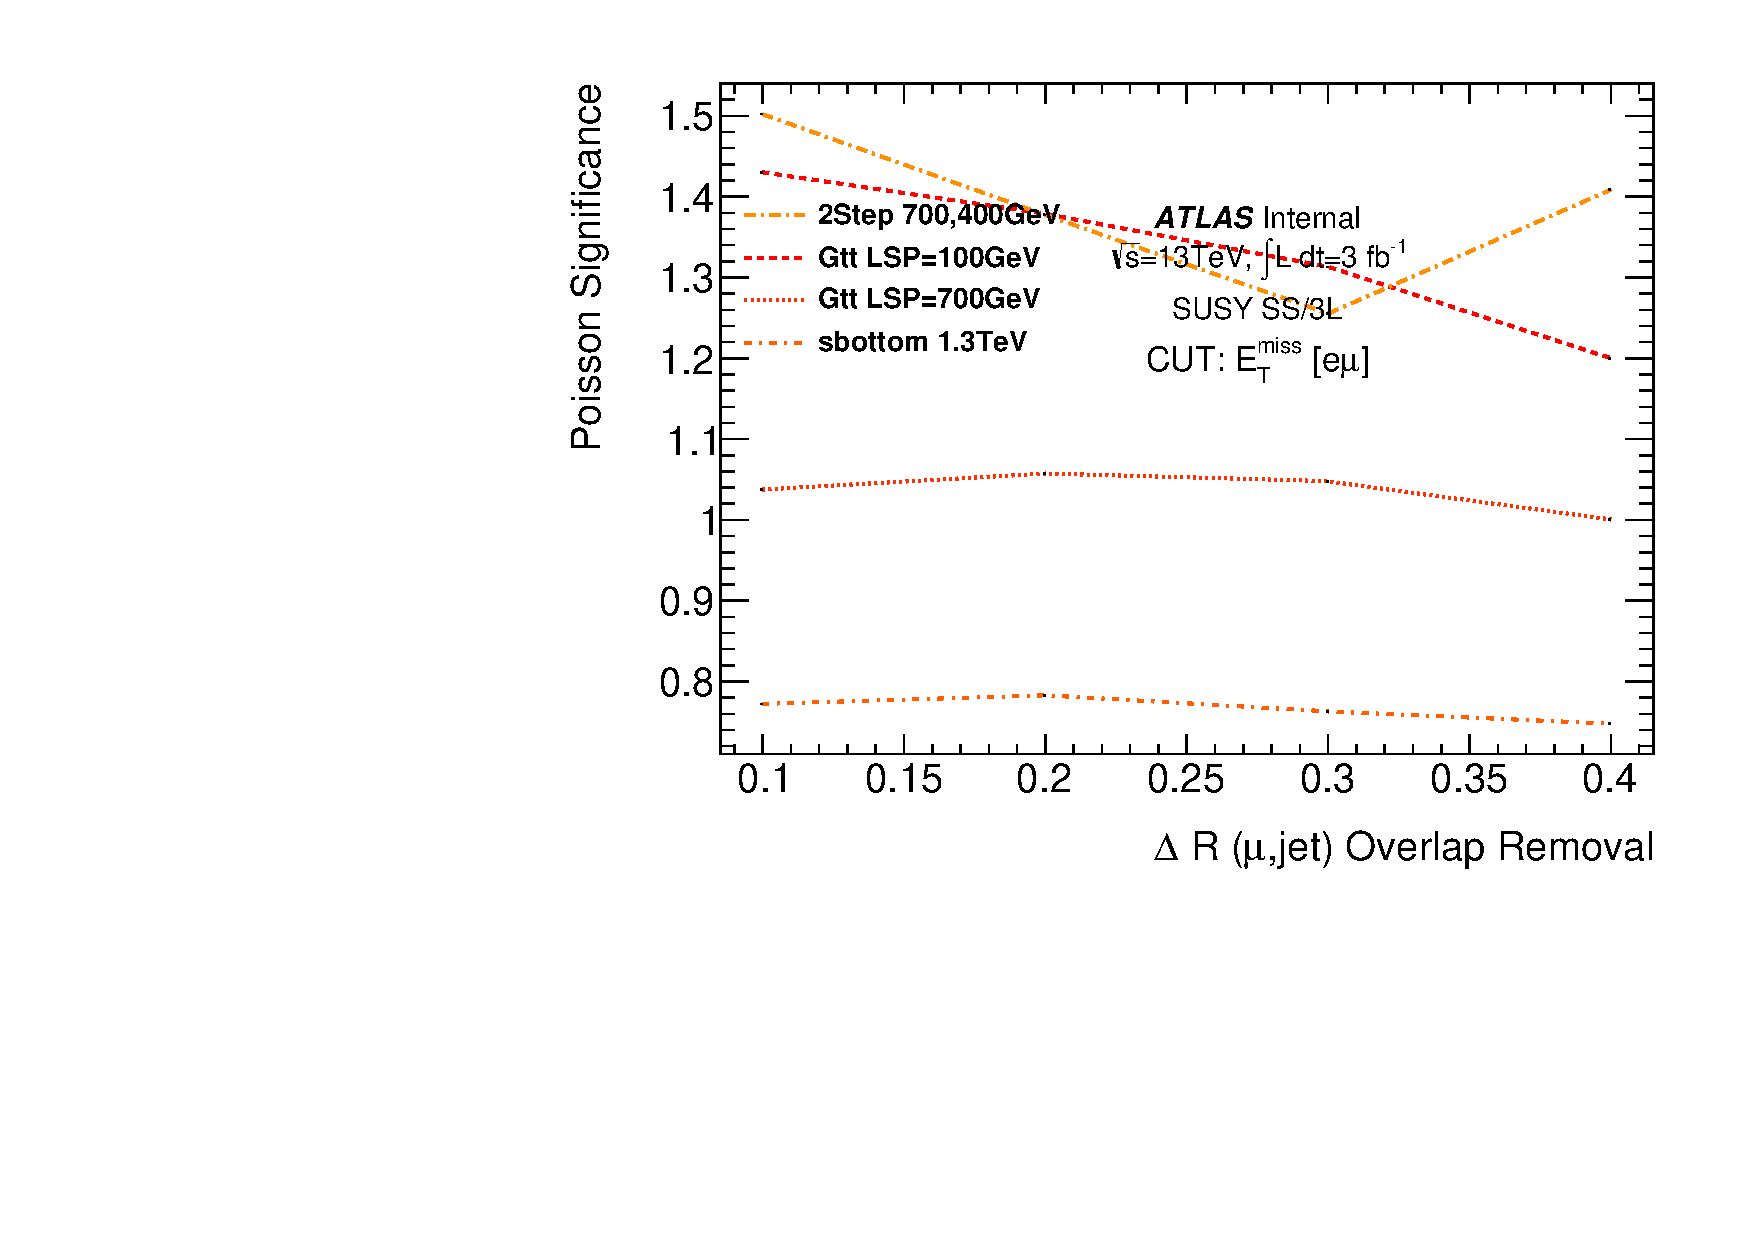
\includegraphics[width=0.45\textwidth]{OVERLAPREMOVAL/plot_significance_em.pdf} 
%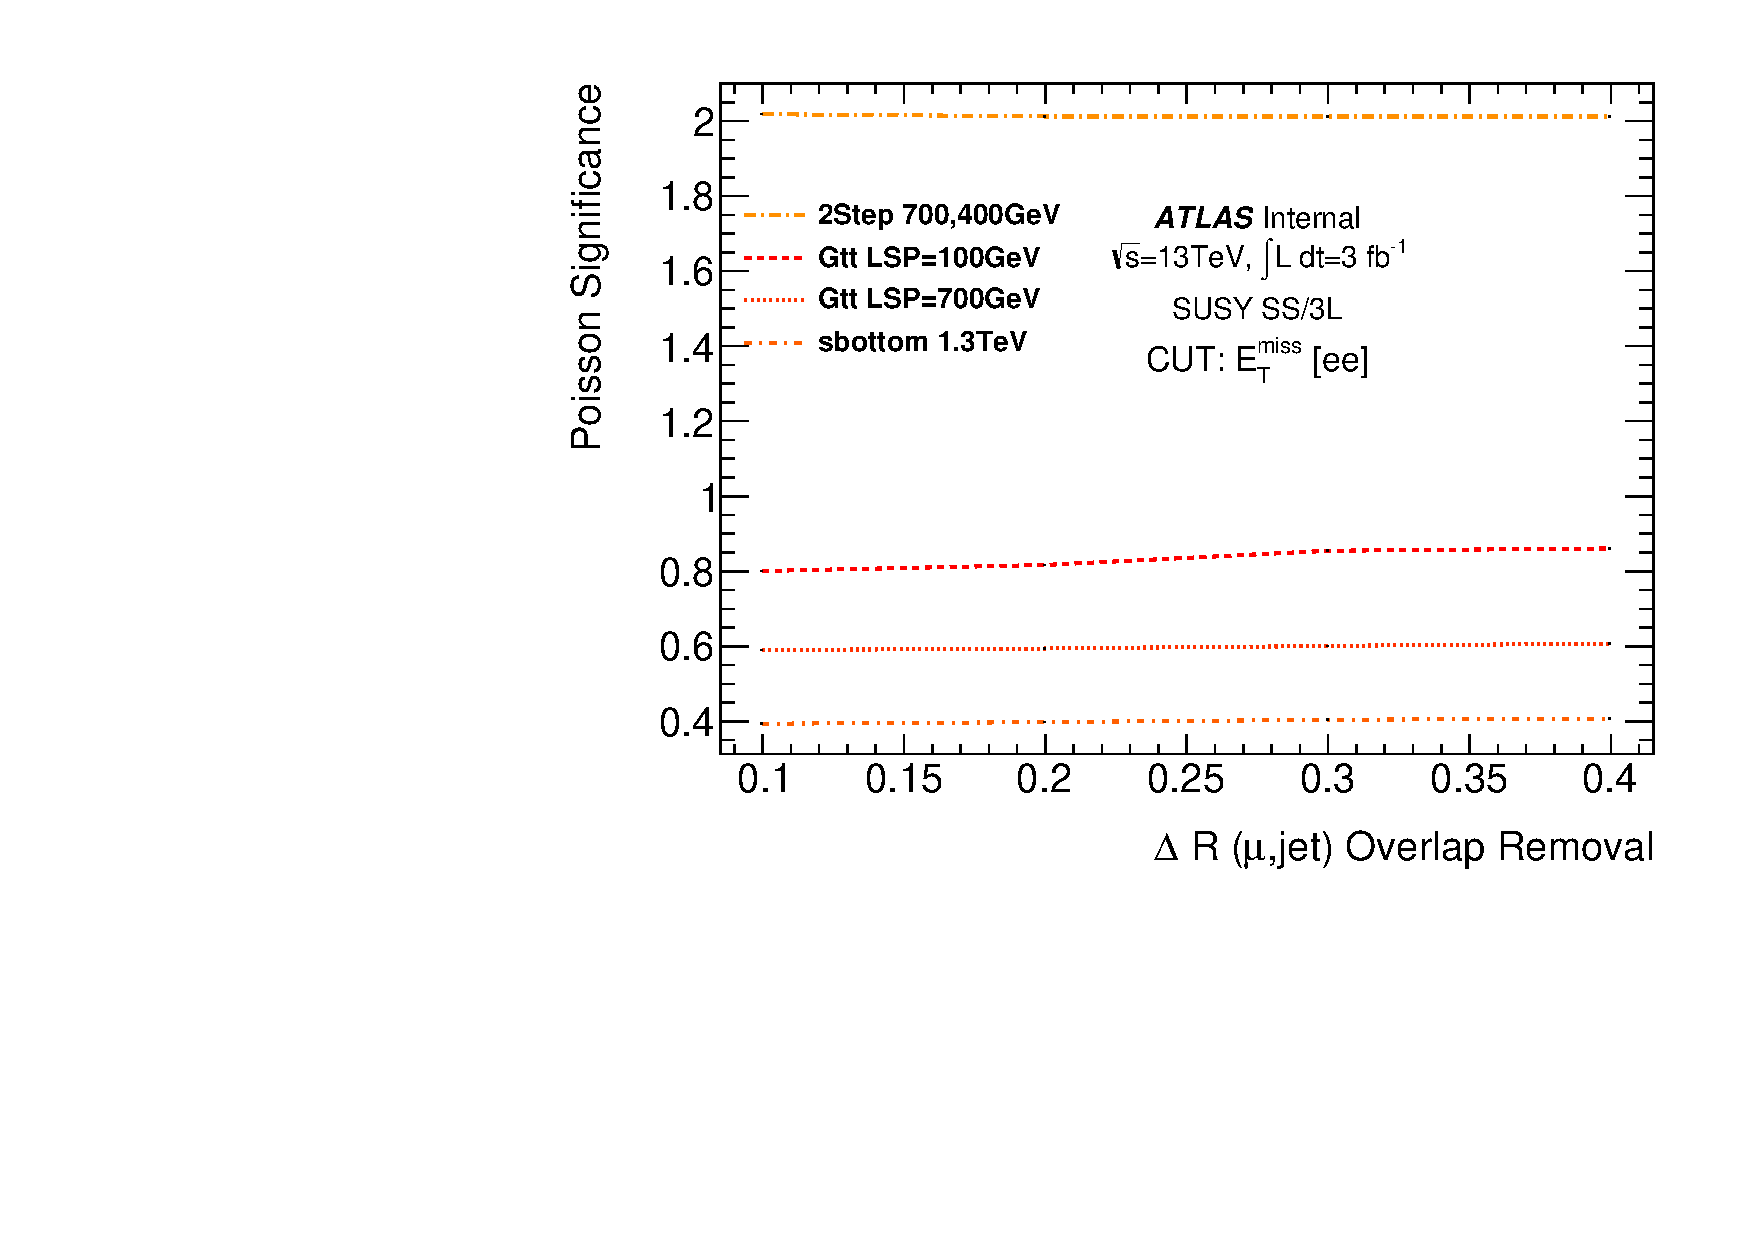
\includegraphics[width=0.45\textwidth]{OVERLAPREMOVAL/plot_significance_ee.pdf} 
%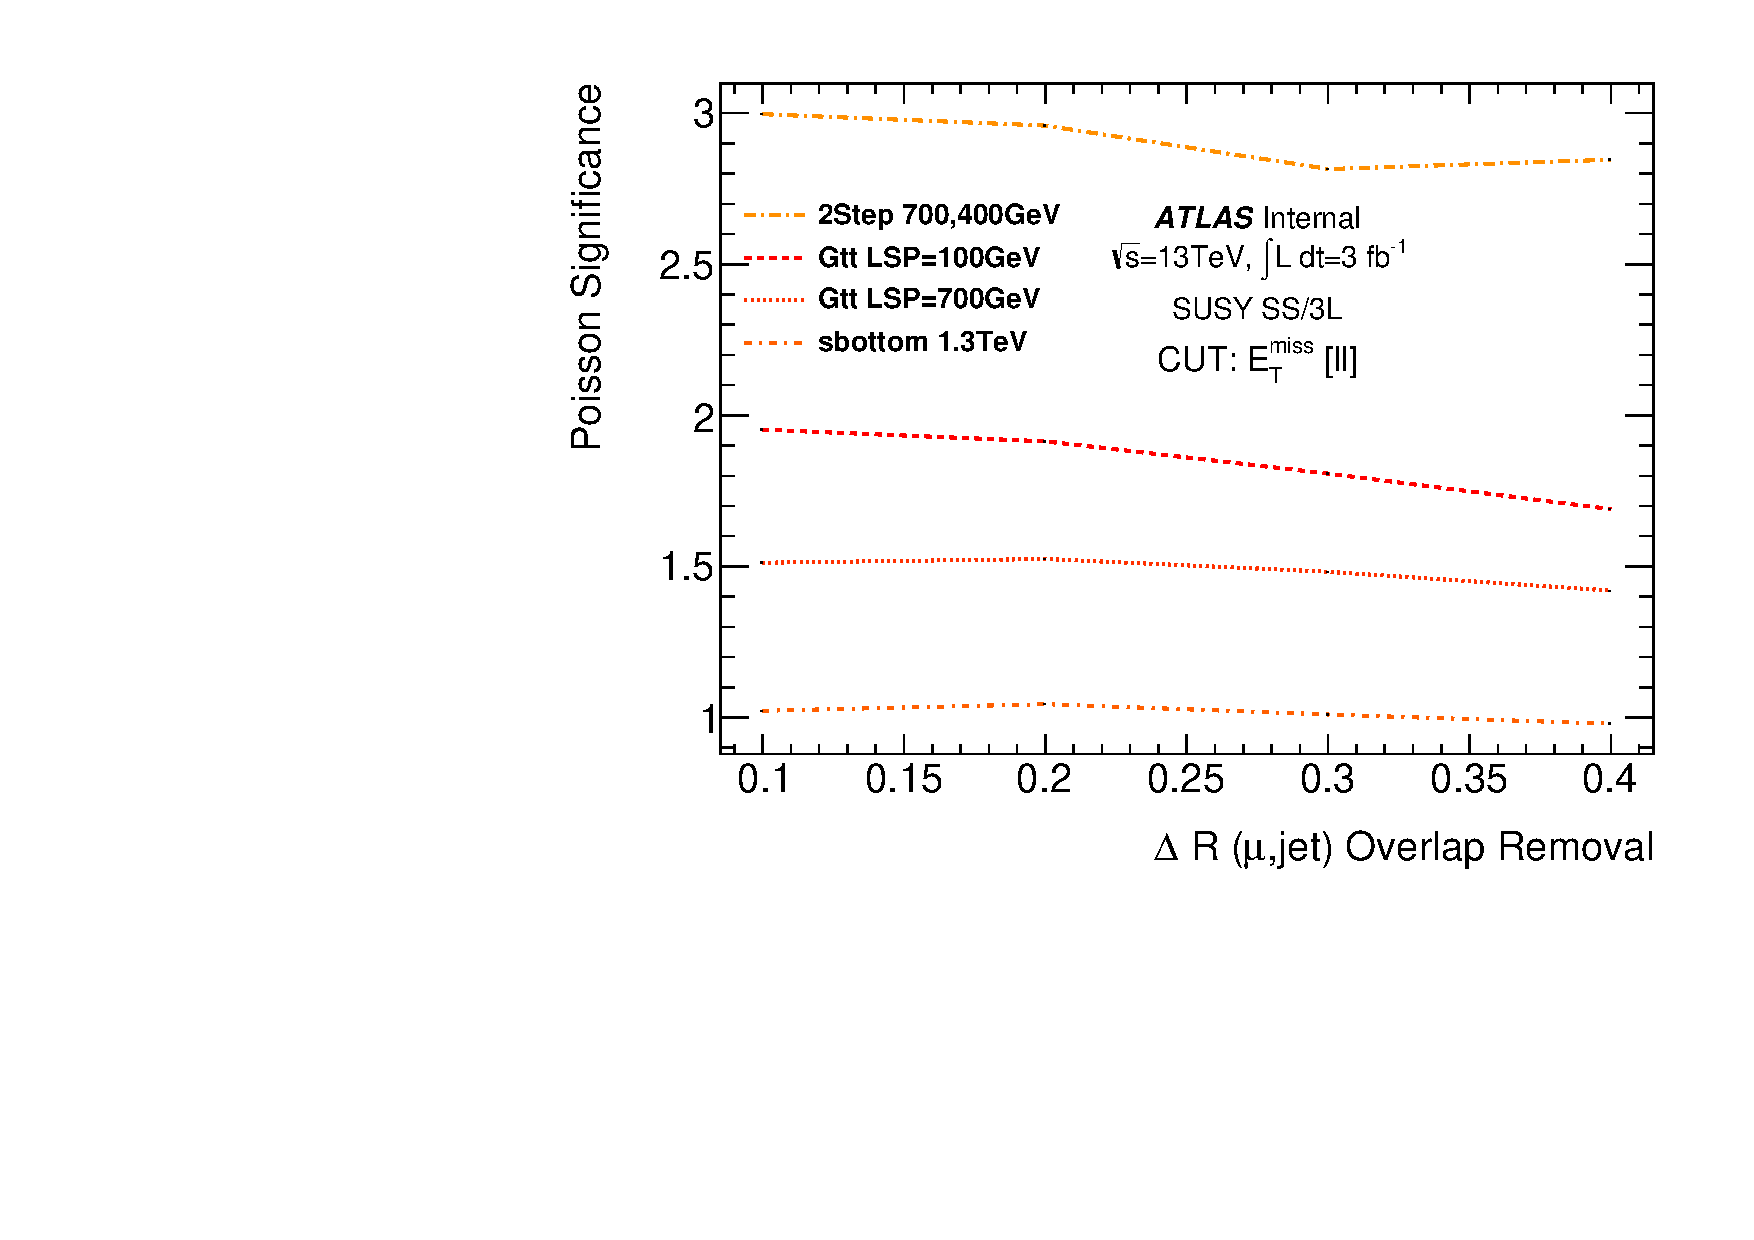
\includegraphics[width=0.45\textwidth]{OVERLAPREMOVAL/plot_significance_ll.pdf} 
%\end{center}
%\vspace{-0.2cm}
%\caption{Discovery significance for an assumed integrated luminosity of 3~fb$^{-1}$, for different choices of cone separation used for the muon-jet object overlap removal in various signal models. 
%Top figures display the significance for the muon-related channels ($\mu\mu$ and $e\mu$) and bottom figues illustrate the effect on the $ee$ channel as well as the flavour combination.}
%\label{fig:OR_significance}
%\end{figure}
%
%The studies seem to favor a choice of a $\Delta R$ of 0.2.  


\subsection{Missing transverse energy}
\label{sec:objects_met}

The missing transverse energy (\met) is rebuilt using the xAOD container ``MET\_RefFinal'' as input and using the calibrated electron, muon and jet objects 
(and baseline photons according to SUSYTools definitions). 
In this version of the analysis, the track soft term is used for building the \met\ following the defaults in SUSYTools-00-07-17.


\subsection{Lepton truth matching}
\label{sec:truth_matching}

In several studies presented in this document, 
a lepton truth matching strategy is applied to distinguish the lepton originating from prompt decays of gauge boson or SUSY particles 
from non-prompt leptons originating from semileptonic $b$-decays, photon conversions or fakes. 
This strategy largely relies on the information from the {\tt MCTruthClassifier} tool. 
However, the latter does not always allow to properly classify electrons originating from a photon conversion, 
where it is important to fully understand the origin of the photon and its possible proximity to a prompt electron 
(FSR, brehmsstrahlung, which is the main mechanism leading to charge-flip electrons). 
In these cases, we complete this information by a matching within a cone of $\Delta R <0.1$ with truth prompt electrons, 
which are identified as the decays of heavy bosons ($W$, $Z$, $h$) or SUSY particles. 
This is however only possible in MC generators storing intermediate resonances in the event record, 
i.e. notably MC samples in which decay chains are handled by Pythia. 

\FloatBarrier



\section{Event selection}
\label{sec:evtsel}

\subsection{Trigger studies}
\label{sec:trigger}
The trigger strategy for the analysis in Run-2 is similar to the one used in the Run-1 version. There, a combination of \met , 
single-lepton and di-lepton triggers was used for the selection of events in the signal region and control distributions. The triggers were checked consecutively starting with the \met\ trigger, followed by the single lepton trigger and the dilepton triggers, until one of the triggers is passed by the event. Offline cuts on the missing energy and the \pt\ of the triggered objects were applied to ensure to be on the efficiency \textit{plateau} of the corresponding trigger.

For Run-2 the triggers to be used are also missing energy and single- and di-lepton triggers. The lepton trigger menu includes triggers selecting isolated and non-isolated leptons as well as dilepton triggers selecting mixed-flavor lepton events. 
The following triggers have been regarded as important for this analysis and were used for further studies on performance and efficiency:

\begin{itemize}
\item Single-lepton triggers: \texttt{HLT\_mu26, HLT\_mu50, HLT\_mu24\_imedium, HLT\_mu26\_imedium}, 

\texttt{HLT\_e20\_medium, HLT\_e60\_medium, HLT\_e24\_tight\_iloose, HLT\_e26\_tight\_iloose}

\item Di-lepton triggers: \texttt{HLT\_2m10, HLT\_2mu14, HLT\_2e12\_loose\_L12EM10VH, HLT\_2e17\_loose, HLT\_e17\_loose\_mu14}

\item Multi-lepton triggers \texttt{HLT\_3m6, HLT\_e12\_loose\_2mu10}

\item \met\ triggers: \texttt{HLT\_xe60, HLT\_xe70, HLT\_xe100, HLT\_xe100\_cell}

\end{itemize}

The performance of these triggers has been investigated by running the analysis 
on dedicated $Z \rightarrow \mu \mu$, $Z \rightarrow ee$ and $t \bar{t}$ Monte 
Carlo samples with several trigger applications.
For each object triggered, an offline cut on the object \pt\ or the \met\ is applied to ensure the full efficiency of the trigger in the selected event. A geometrical $\Delta R$ matching between the lepton triggers fired and the signal leptons reconstructed in each event is applied in order to confirm that the according trigger was activated by one of the signal leptons found in the analysis. 


\subsubsection{Monte Carlo samples and software framework}

The trigger studies were performed with the latest available releases of the ATLAS software framework and the latest Monte Carlo productions. The analysis code was setup with the \texttt{AnalysisBase} framework (2.3.8 branch for rel.20 ATLAS software). The object selection was done by using the \texttt{SUSYTools-00-06-03} package which provides the current recommendations for selection of signal and baseline objetcs. 

The Monte Carlo samples used for these studies are validation samples produced with the 20.1.4.3 MC15 ATLAS software release (no pileup). 

\begin{itemize}

\item $t \bar{t}$ sample: 

\texttt{valid3.110401.PowhegPythia\_P2012\_ttbar\_nonallhad.recon.AOD.e3099\_s2578\_r6540}

\item $Z \rightarrow \mu \mu$ sample:  

\texttt{valid3.167826.Sherpa\_CT10\_ZmumuMassiveCBPt280\_500\_CVetoBVeto.recon.AOD.e3099\_s2578\_r6540}

\item $Z \rightarrow e e$ sample: 

\texttt{valid3.147406.PowhegPythia8\_AZNLO\_Zee.recon.AOD.e3099\_s2578\_r6540}

\end{itemize}

\subsubsection{Total event yields}

The total event yields for the test MC samples and different trigger configurations was measured. The yields are shown in Fig.~\ref{fig:events} for the $t \bar{t}$ Monte Carlo sample and for the $Z \rightarrow \mu \mu$, $Z \rightarrow ee$ samples respectively. The trigger performance is as expected: while for $Z \rightarrow \mu \mu$ Monte Carlo, the muon triggers select most of the events, for $Z \rightarrow ee$ the electron triggers do. For $t \bar{t}$ Monte Carlo, the muon- and electron triggers have similar selection rates, and most events are selected by applying \met\ triggers.

\begin{figure}[htb!]
\centering
\subfigure{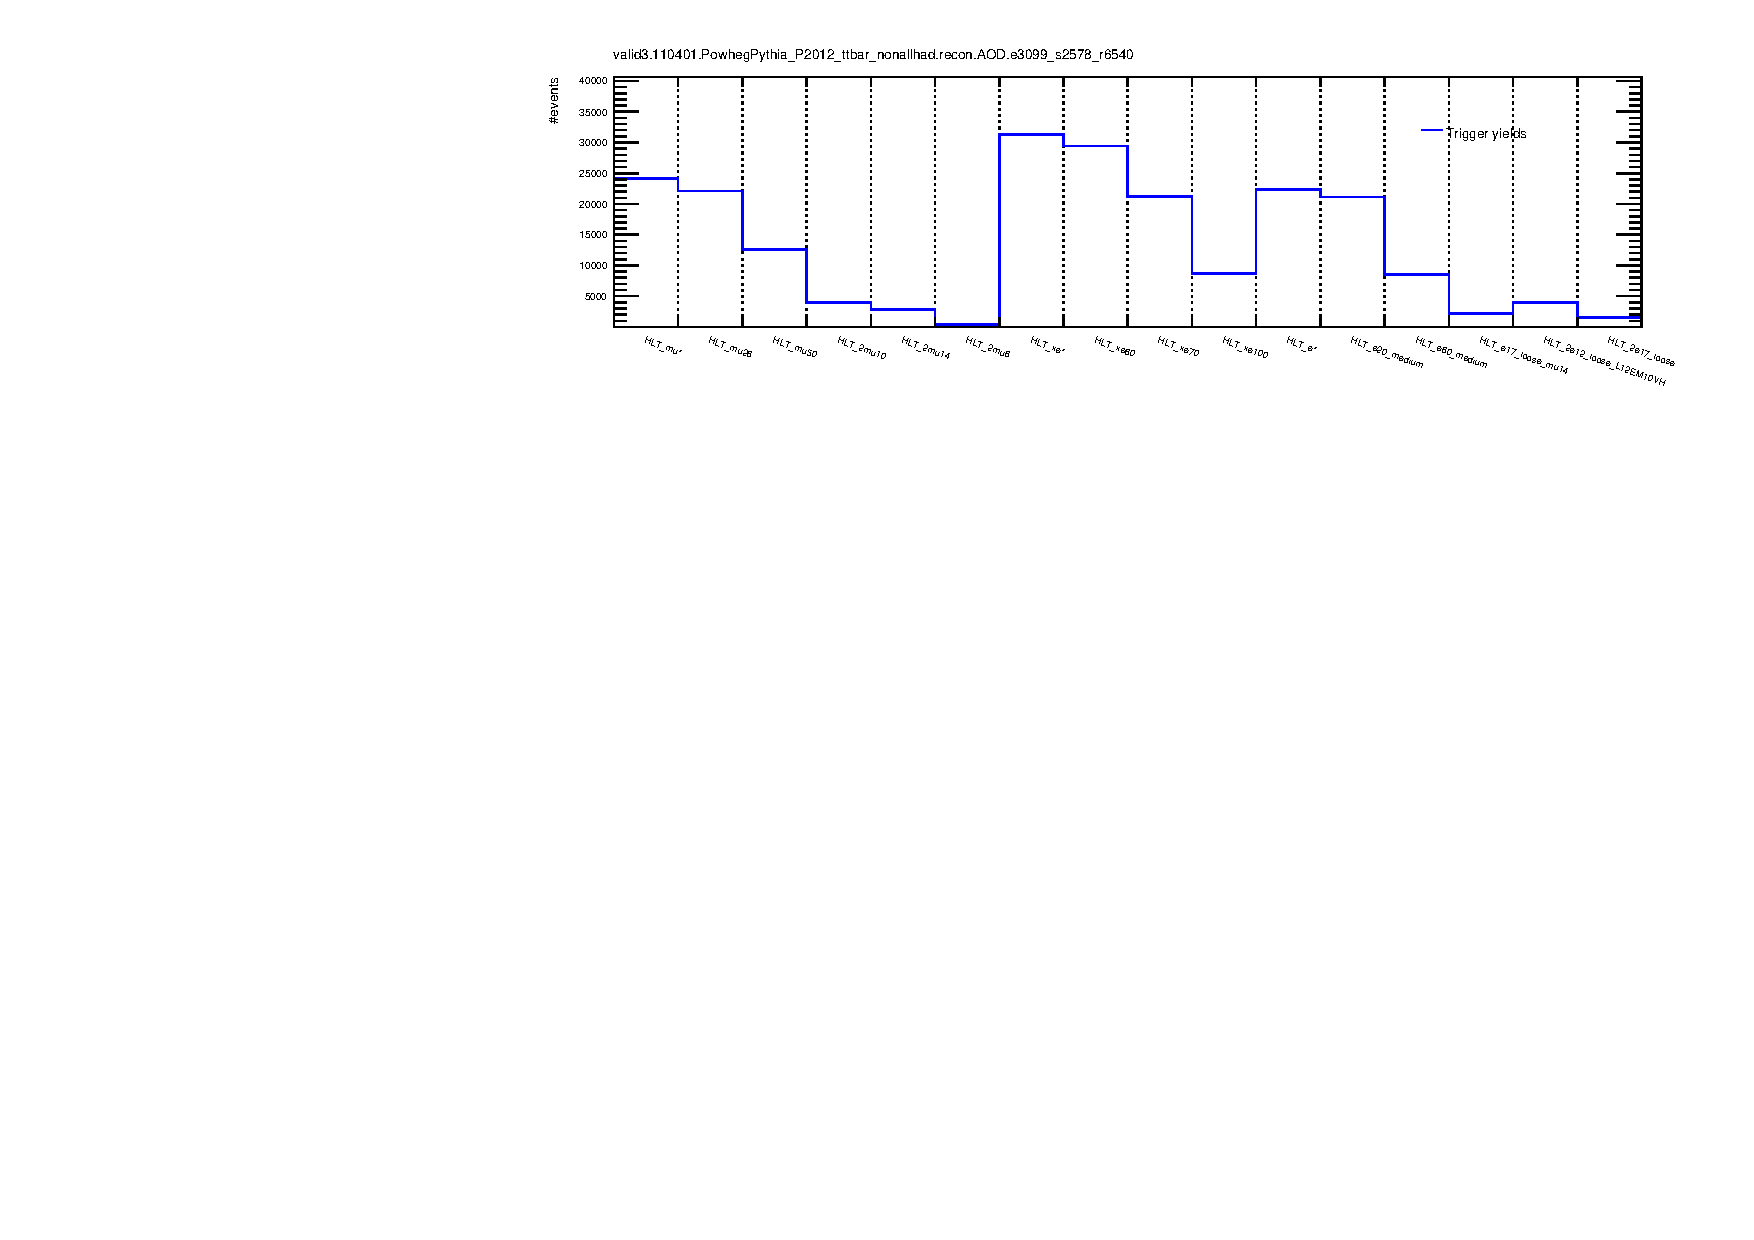
\includegraphics[width=1.\textwidth]{TRIGGER/Events_ttbar}}
\subfigure{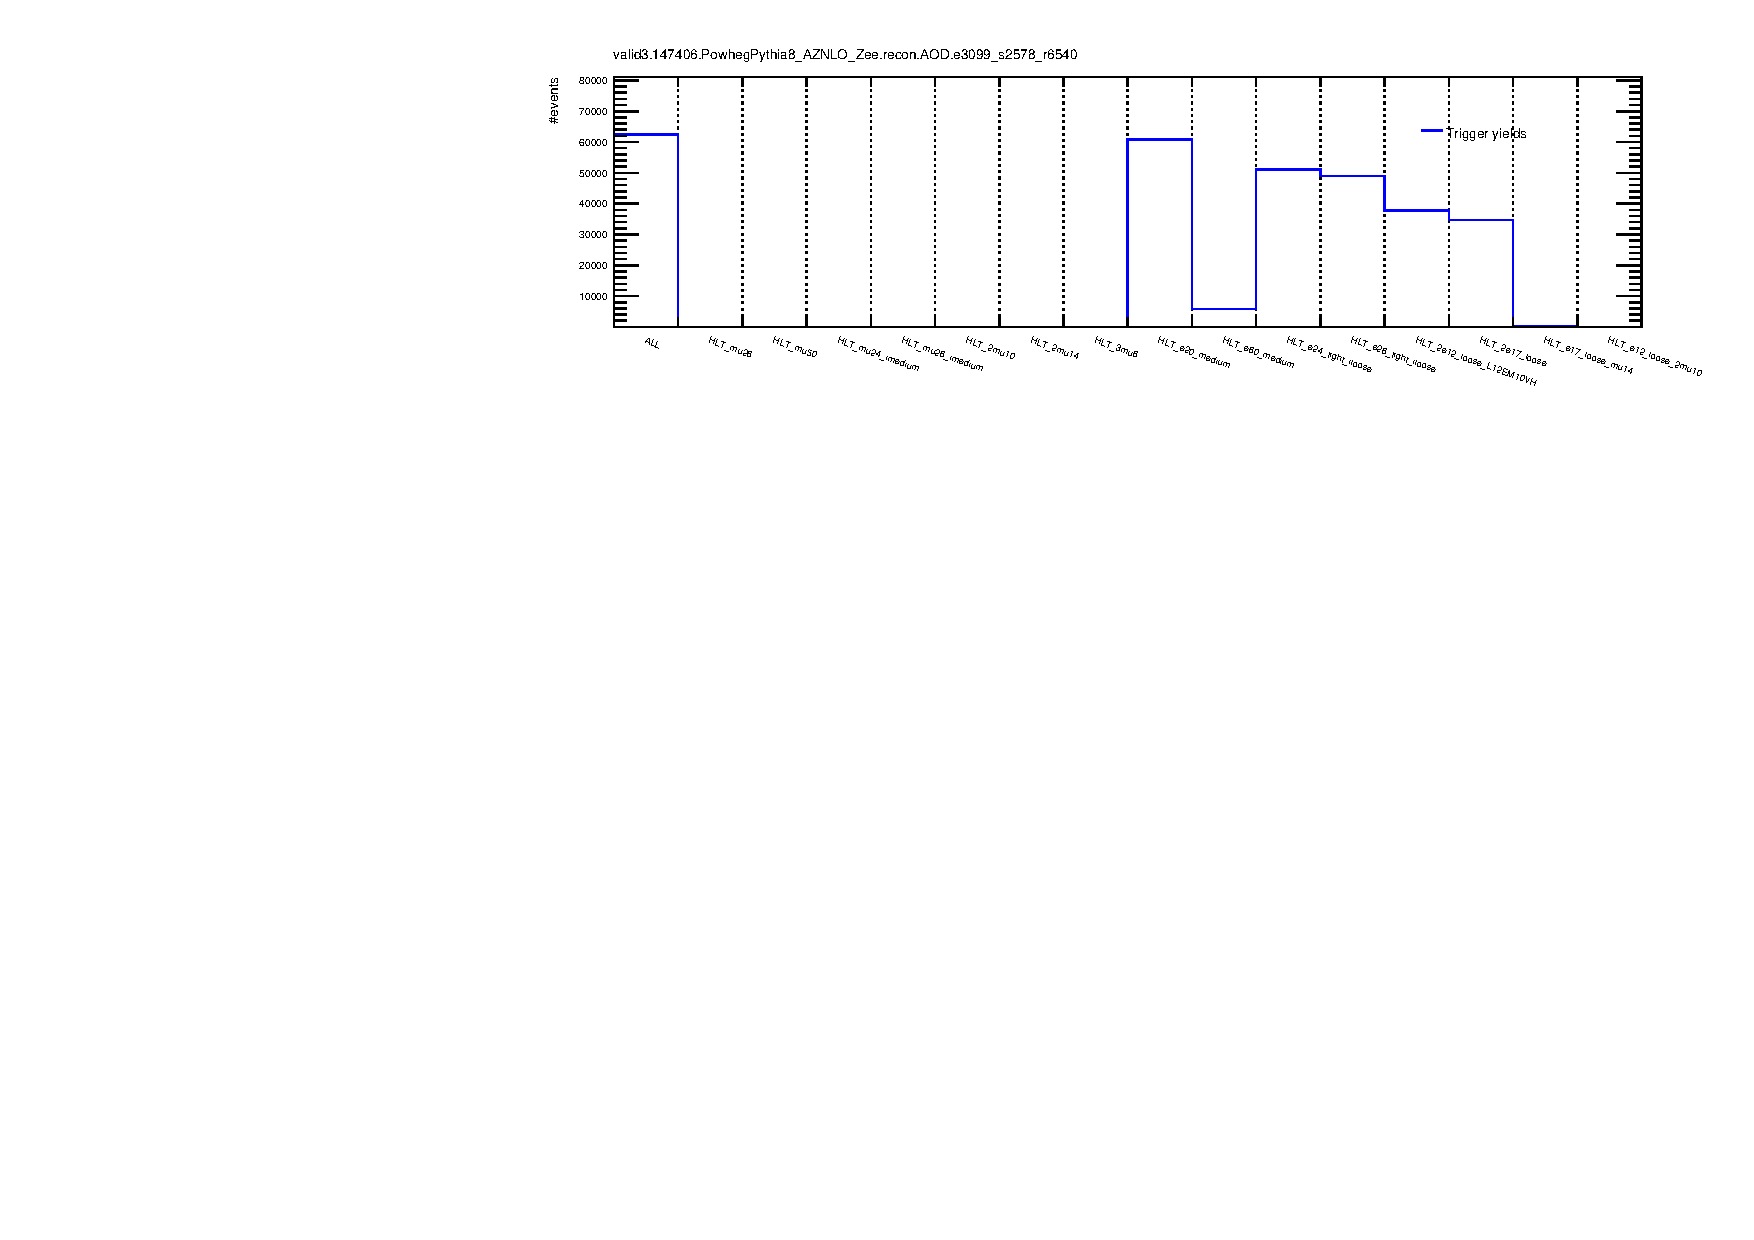
\includegraphics[width=1.\textwidth]{TRIGGER/Events_Zee}}
\subfigure{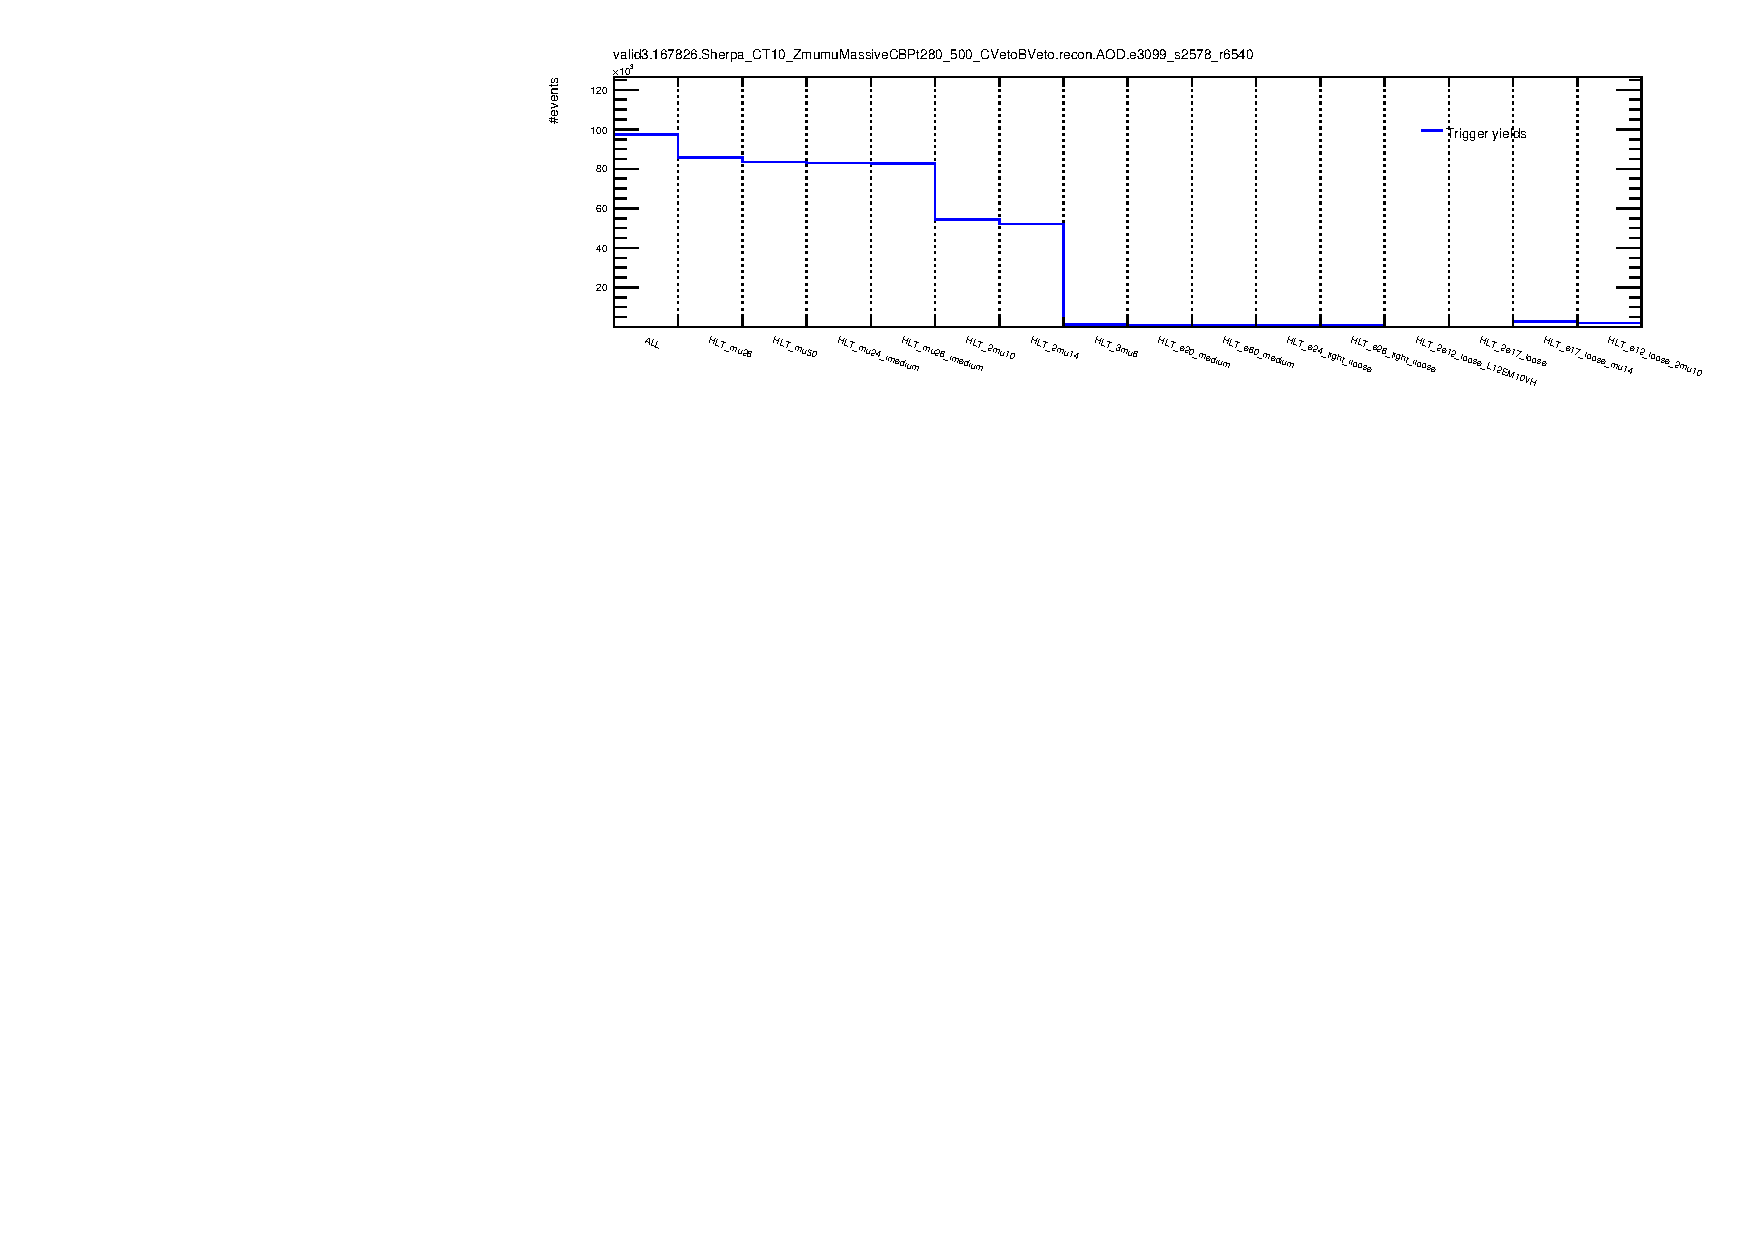
\includegraphics[width=1.\textwidth]{TRIGGER/Events_Zmumu}}
\caption{Total event yields for the $t \bar{t}$ sample (top) and for the $Z \rightarrow \mu \mu$ (middle), $Z \rightarrow ee$ (bottom) samples. On the x-axis the different triggers (or trigger configurations) are shown.}
\label{fig:events}
\end{figure}

\subsubsection{Efficiencies}

The trigger efficiency in Monte Carlo can be obtained by dividing the number of triggered events by the total number of events. The efficiencies have been calculated separately for single-lepton, dilepton triggers and for \met\ triggers. The results for some examples are shown in Fig.~\ref{fig:eff_singlelepton} for single lepton triggers and for dilepton and \met\ triggers on Fig.~\ref{fig:eff_dilepton_met}. Further efficiency plots can be found in Appendix~\ref{app_trigger}. The turn-on curves for the single-lepton and dilepton triggers show the expected evolution. The efficiency at the trigger plateau is between 95\% - 98\% for single-lepton and around 90\% for dilepton triggers. For the \met\ trigger, the turn-on is slower with respect to the quoted online threshold. It reaches its efficiency plateau if \met\ $>$ 250 GeV and the efficiency value in plateau is around 80\%.  

\begin{figure}[htb!]
\centering
\subfigure{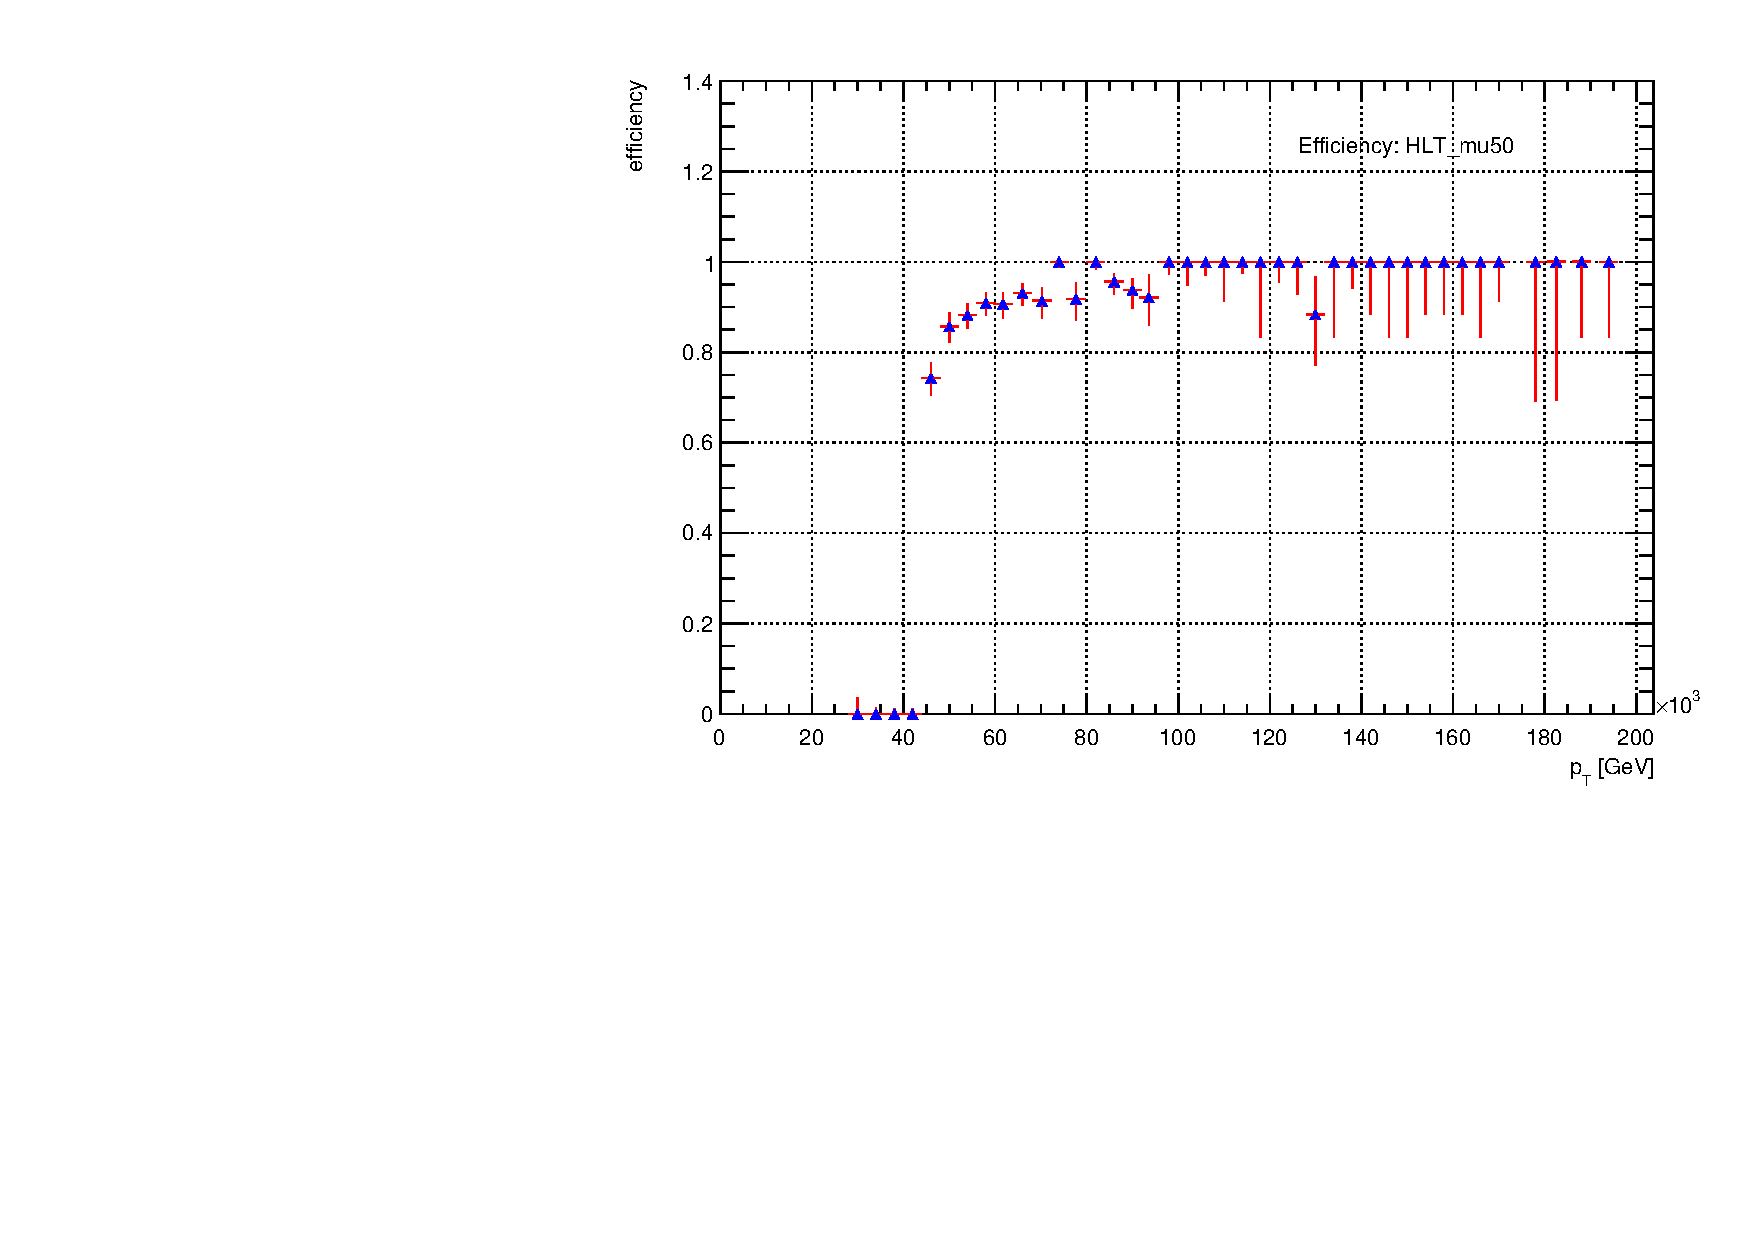
\includegraphics[width=0.48\textwidth]{TRIGGER/Eff_HLT_mu50}}
\subfigure{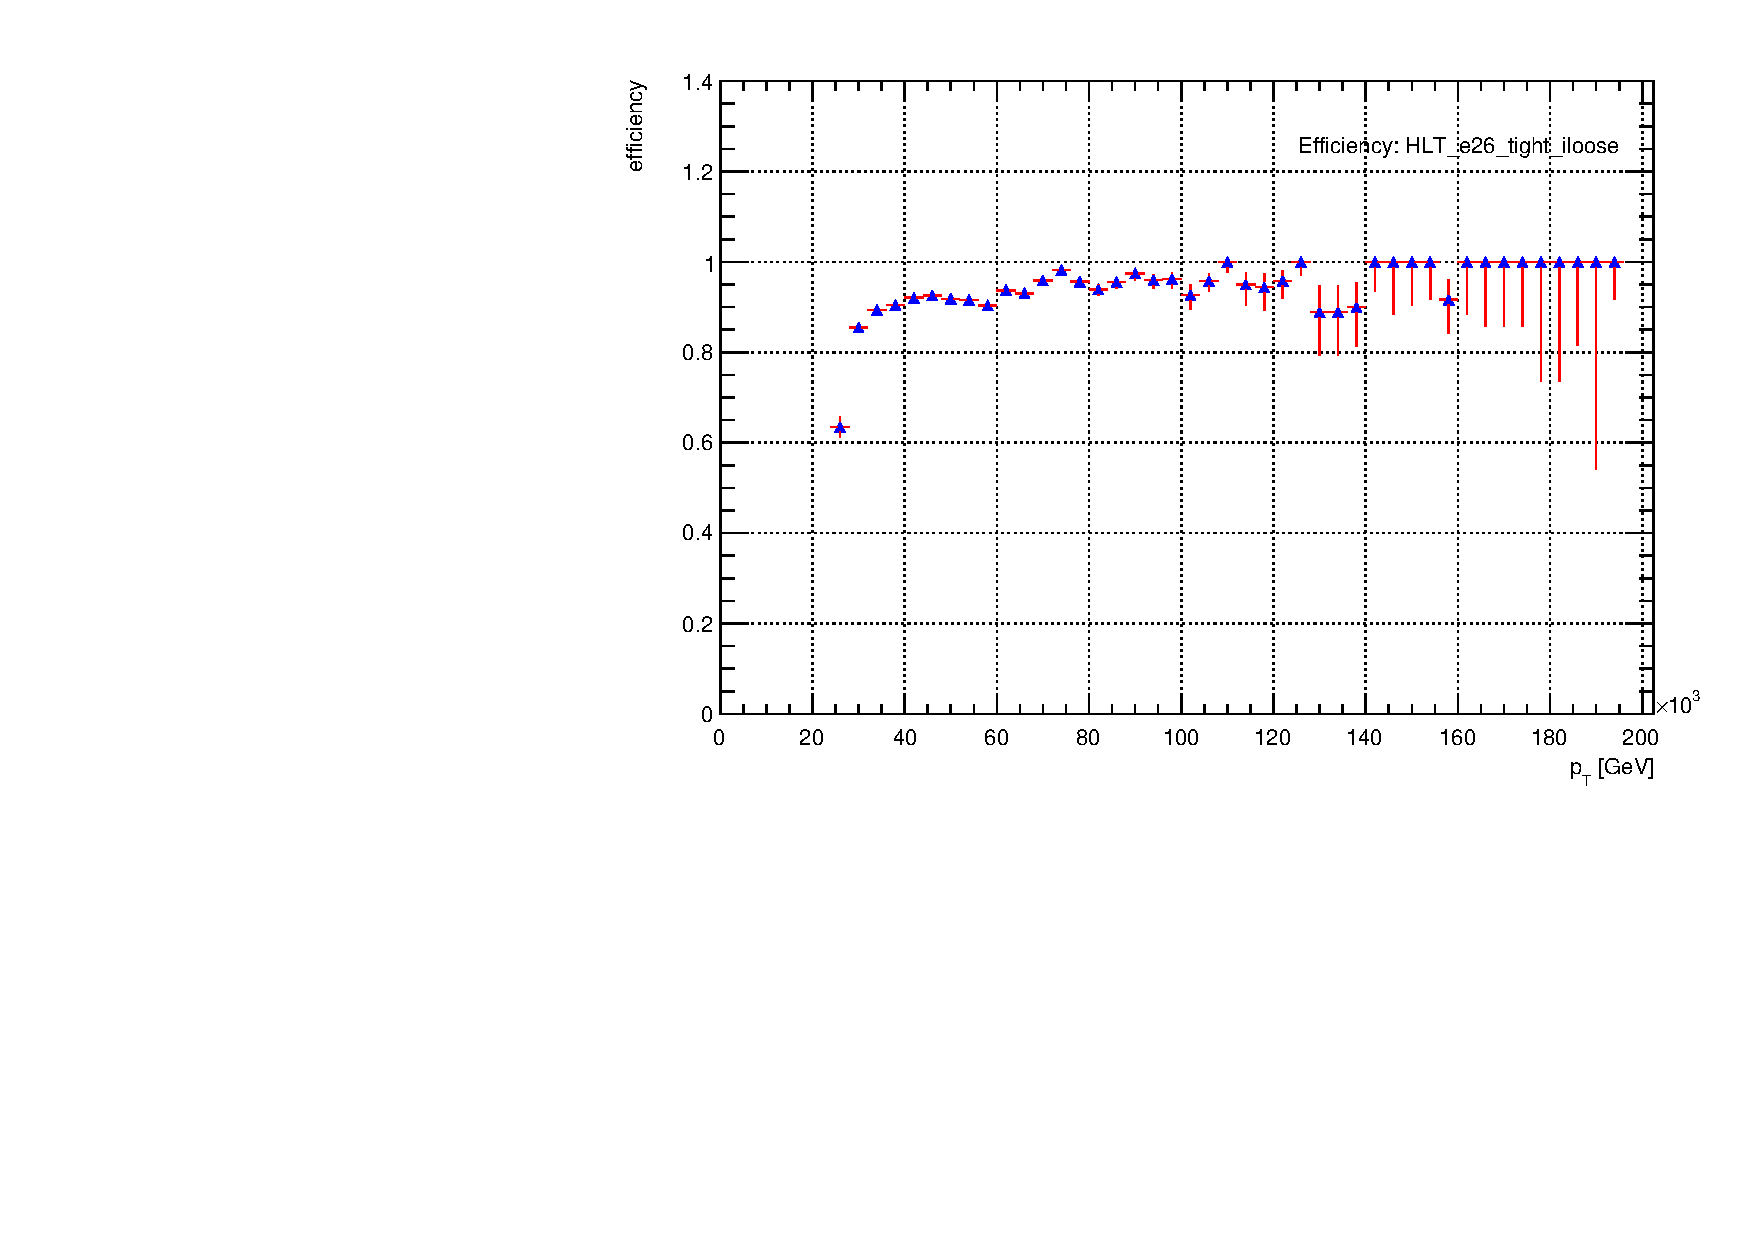
\includegraphics[width=0.48\textwidth]{TRIGGER/Eff_HLT_e26_tight_iloose}}
\caption{Trigger efficiencies for \texttt{HLT\_mu50} and \texttt{HLT\_e26\_tight\_iloose} versus \pt\ of the leading lepton. 
%The turn-on curves of the triggers are close to the expected threshold of the online efficiency. The efficiency on the trigger plateau is around 95\%.
}
\label{fig:eff_singlelepton}
\end{figure}

\begin{figure}[htb!]
\centering
\subfigure{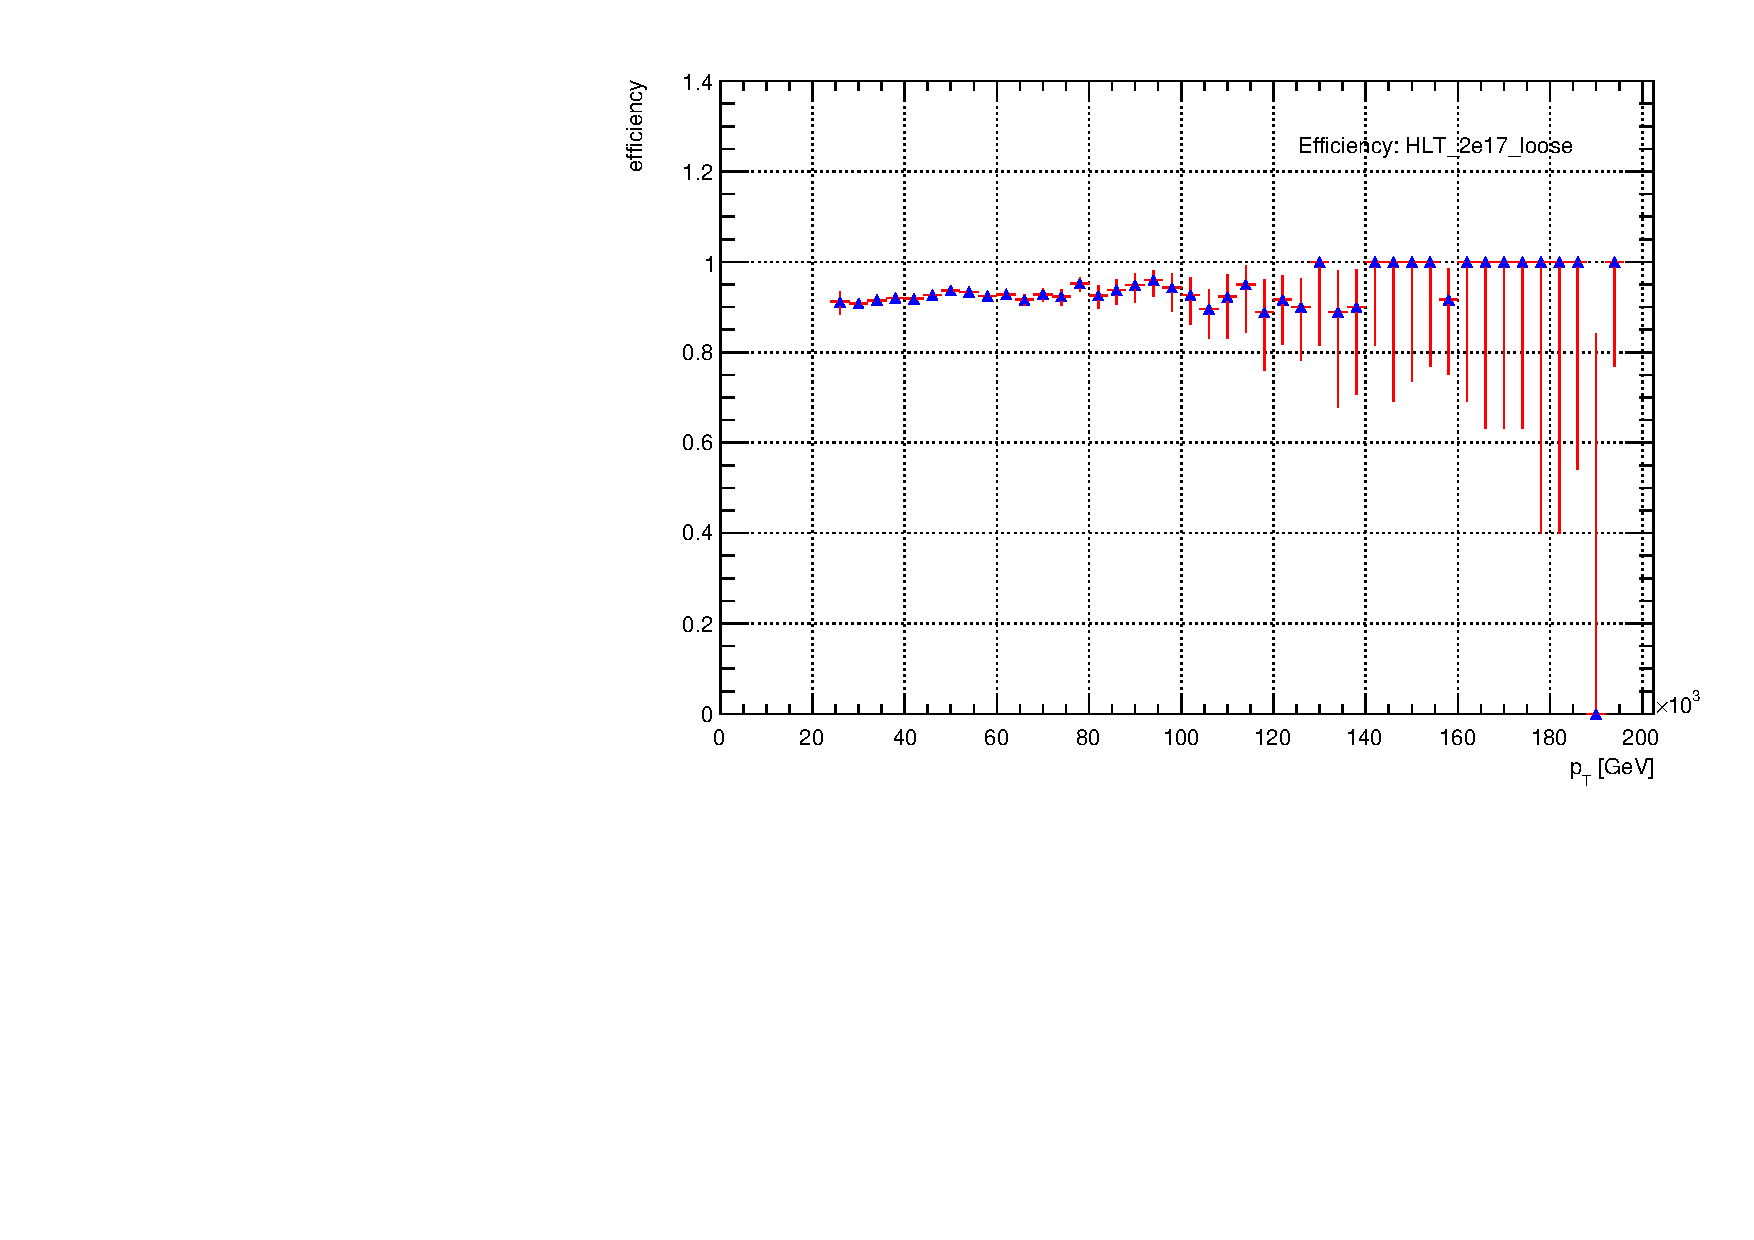
\includegraphics[width=0.48\textwidth]{TRIGGER/Eff_HLT_2e17_loose}}
\subfigure{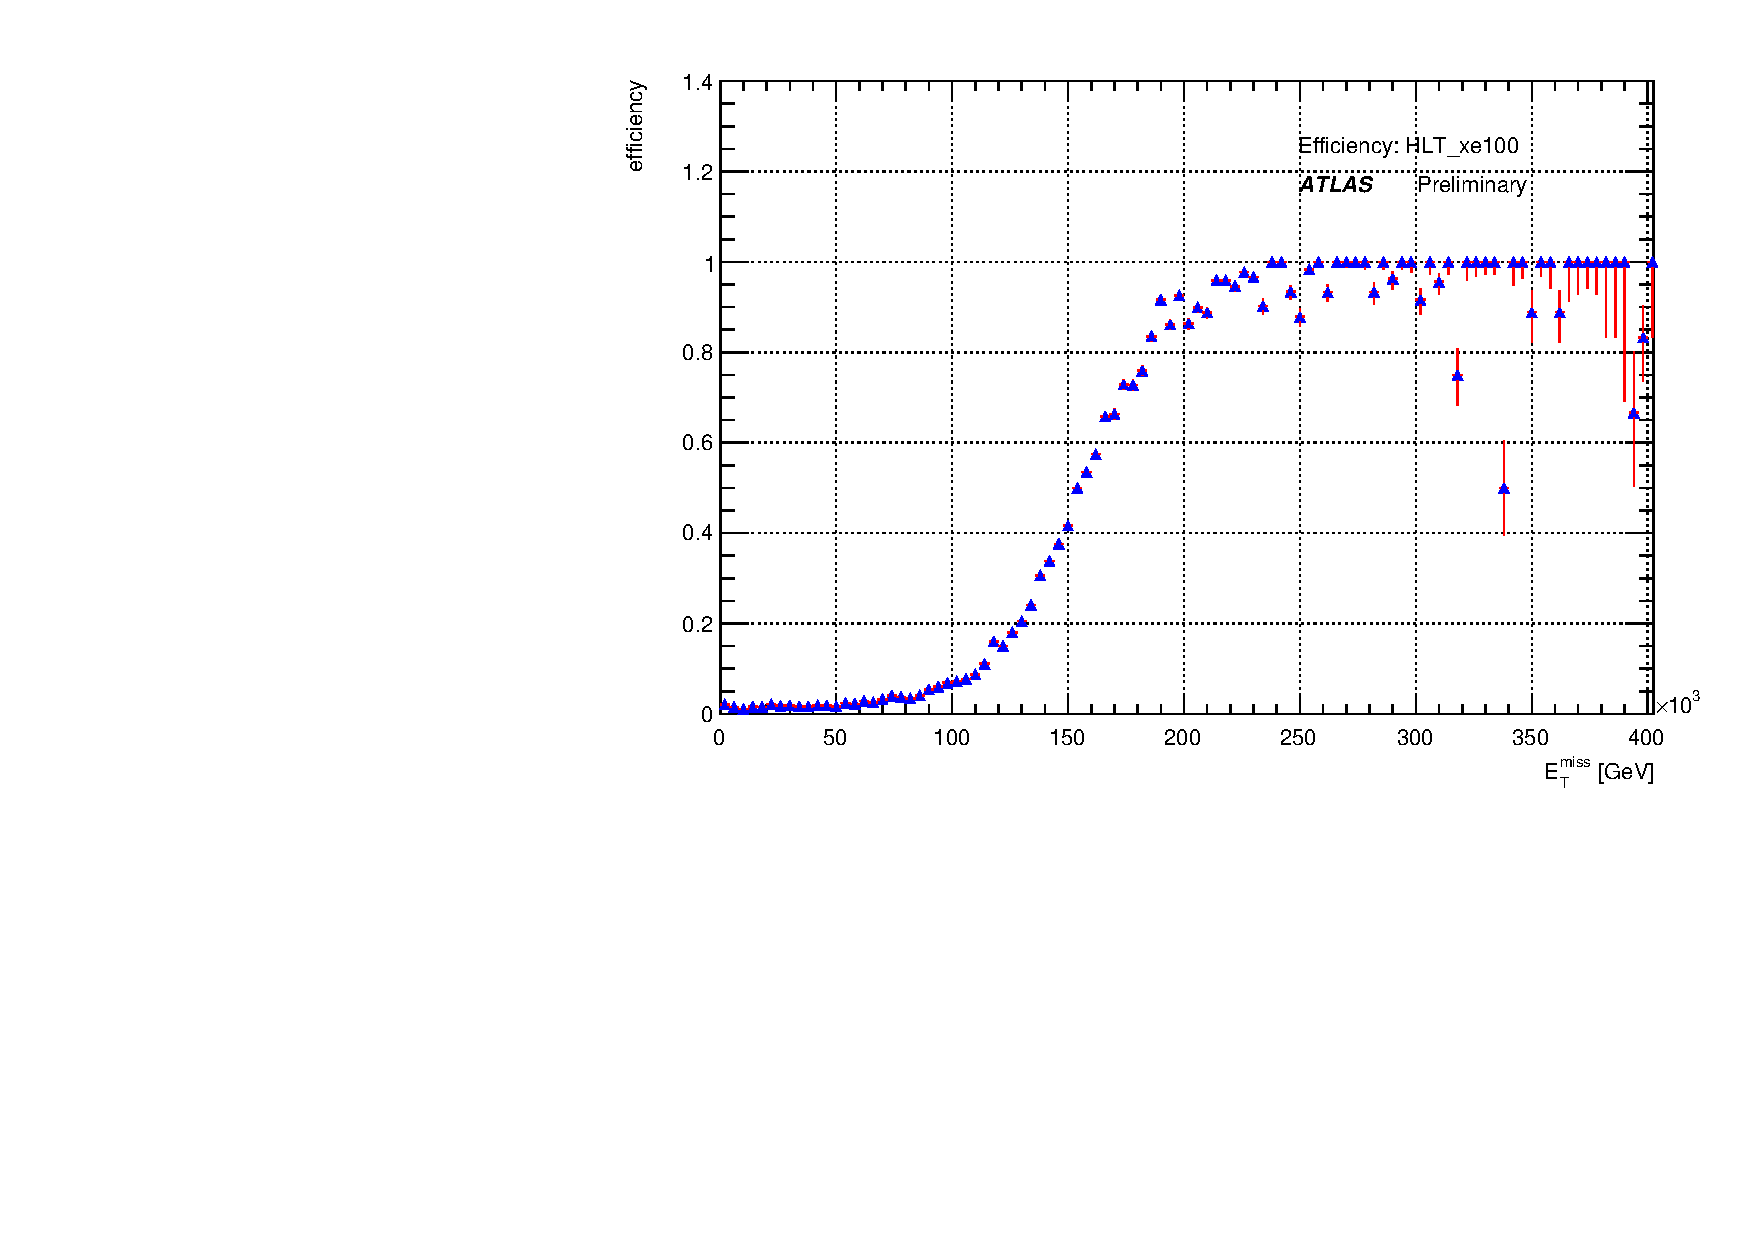
\includegraphics[width=0.48\textwidth]{TRIGGER/Eff_HLT_xe100}}
\caption{Trigger efficiencies for \texttt{HLT\_2e17\_loose} (left) and \texttt{HLT\_xe100} (right). The efficiency for the dilepton trigger is plotted against the \pt\ of the leading electron while the efficiency of the \met\ trigger is plotted against the corrected missing energy value. %Both triggers show the expected performance on the efficiency plateau. The dilepton trigger reaches an efficiency of around 90\%. For the \met\  trigger, the turn-on is slower. At the plateau it reaches also an efficiency of around 90\%.
}
\label{fig:eff_dilepton_met}
\end{figure}



\subsection{Event pre-selection}
\label{sec:presel}

%A few general selection criteria based on data quality, detector quality flags are the following:
\par A sample of two same-sign or three leptons is selected applying the following criteria:
\begin{itemize}
%\item{ \textbf{GRL}: The used GoodRunsList, providing a total
%    luminosity of $\lumi$~\ifb, was \newline
%\small{\texttt{data12\_8TeV.periodAllYear\_DetStatus-v58-pro14-01\_DQDefects-00-00-33\_PHYS\_StandardGRL\_All\_Good.xml}}.}
%\item{ \textbf{Trigger}: The data have been collected using lepton and \met\ triggers, as described in Section \ref{section:trigger}.}
%\item{ \textbf{LAr and Tile Error}: Impact from the noise bursts and data corruption in the LAr and
% Tile calorimeter is reduced by selecting events without an error from
% the quality checks (larError!=2 and tileError!=2). } 
%\item{ \textbf{Incomplete events}: Incomplete events due to the TTC restart procedure are rejected.}

%\item{ \textbf{Fake \met\ Veto}: Events with fake \met\ due to jets
%    pointing to dead TileCal and HEC regions are rejected. This is
%    achieved by vetoing events with at least one
%    jet~\footnote{Anti-k$_{\rm T}$ jets with $R=0.4$ before
%      electron-jet overlap removal are considered for the veto. } satisfying:
%    \newline 
%$\pt > 40\,\GeV\ \&\&\ C_{jet}  > 0.05\ \&\&\ \Delta\phi (\met,jet) <
%    0.3$ \newline where  $C_{jet}$ is the estimated correction factor  
%    for the energy losses estimated using the jet profile. The veto is applied
%    to all events in data and simulation.}
    
\item{ \textbf{Jet Cleaning}: Events are required to pass the
  {\tt{VeryLooseBad}} set of cleaning requirements recommended by Jet-\met\ group \cite{jetcctwiki} 
  and implemented in the {\tt{JetCleaningTool}}. 
An event is rejected if at least one of the pre-selected jets (thus
after jet-electron overlap removal) fails the jet quality criteria. 
The cleaning requirements are intended to remove events where significant energy was deposited in
  the calorimeters due to instrumental effects such as cosmic rays,
  beam-induced (non-collision) particles, and noise. } 
  
\item{ \textbf{Primary Vertex}: events are required to have a primary vertex, that is, one of the reconstructed vertices
   must be labeled as {\tt{xAOD::VxType::PriVtx}}. No additional requirements on the number of tracks in the 
   vertex should be applied as recommended by the Tracking CP group~\cite{vertex_twiki}.
}

\item{ \textbf{Bad Muon Veto}:  Events containing at least one pre-selected muon satisfying $\sigma(q/p)/|q/p| >$ 0.2 before the overlap removal are rejected.}

\item{ \textbf{Cosmic Muon Veto}: Events containing a cosmic muon candidate are rejected. Cosmic muon candidates are selected among pre-selected muons, if they fail the requirements $|z_0| <$ 1.0\,mm and $|d_0| <$ 0.2\,mm, where the longitudinal and transverse impact paramaters $z_0$ and $d_0$ are calculated with respect to the primary vertex.}

\item{ \textbf{At least two leptons}: Events are required to contain
    at least two signal leptons (see Section~\ref{sec:objects} and
    Table \ref{tab:lepdef}) with $p_{\mathrm{T}}
    > 20\,\GeV$ and $p_{\mathrm{T}} > 15\,\GeV$ for the leading and subleading lepton, respectively. 
    If the lepton contains a third lepton with $p_{\mathrm{T}} > 15\,\GeV$ the event is regarded as three-lepton
    event otherwise as a two-lepton event. Once the trigger is fully operative in the MC samples, 
    one or two of the three leptons will be 
    matched to the trigger object
    if the event is classified as passing a single or dilepton trigger.
    The data sample obtained is then divided into three channels depending on the flavor of the two 
    leading leptons ($ee$, $\mu\mu$, $e\mu$).}

\item \textbf{Electron-muon overlap}: For any events containing at least one of
  each of a signal electron and muon, the event is vetoed if $\Delta R(e, \mu) < 0.1$.

\item{ \textbf{Same sign}: If the event is a two-lepton event the two leading leptons have to be of 
    same charge (same-sign).}
\item{ \textbf{Z-veto}: If the event is a three-lepton event all possible opposite-charge same-flavor lepton
    combinations are combined to calculate a mass $M_{\ell\ell}$. The event is rejected if one of the calculated mass
    is close to the $Z$-mass, i.e.~$84 < M_{\ell\ell} <  98\,\mathrm{GeV}$.}
\item{ \textbf{Invariant mass}: Events with $M_{\ell\ell} < 12\,\GeV$ are
    rejected to avoid heavy flavor meson resonances. In three-lepton events, the invariant mass $M_{\ell\ell}$ is calculated from the 
    two leading leptons. }
\end{itemize}


The following event variables are also used in the definition of the signal and validation regions in the analysis:

\begin{itemize}
\item The inclusive effective mass \meff~ defined as the scalar sum of
  the signal leptons \pt (see Table~\ref{tab:lepdef}), all signal jets \pt\ (see Table~\ref{tab:jetsdef}) and \met;
\item The transverse mass \mt\ computed from the leading lepton and
\met\ as \newline $\mt = \sqrt{2 \cdot \pt^l \cdot \met \cdot (1 - cos(\Delta \phi(l, \met )))}$;
\end{itemize}

\section{Signal region definition}
\label{sec:sr}
\label{sec:SignalRegDef}

The definitions of the signal regions have been studied to provide an optimal performance for $\sqrt s=13$ TeV collisions and a low integrated luminosity (2-4~\ifb). 
This optimization process was first performed with DC14 MC samples, and was then refined with the more accurate MC15 samples and close-to-final object definitions. 
We chose to categorize the signal regions based on their $b$-jet multiplicity, in continuation of the approach sustained in the Run-1 analysis: 
\begin{itemize}
\item[$\bullet$] Signal region(s) with at least one $b$-jet (``SR1b''): these selections target signal scenarios involving top or bottom quarks, 
mostly related to third-generation squarks, such as the benchmark process $\sbot\sbot^*\to t\bar t\tilde\chi_1^+\tilde\chi_1^-$. 
\item[$\bullet$] Signal region(s) with at least three $b$-jets (``SR3b''): these selections target signal scenarios involving many top or bottom quarks, 
such as the benchmark process $\gluino\gluino\to t\bar tt\bar t\ninoone\ninoone$, 
and with their intrinsically very low background are particularly well suited for scenarios with compressed mass spectra. 
\item[$\bullet$] Signal region(s) with a $b$-jet veto (``SR0b''): these selections allow to increase the sensitivity to signal scenarios without bottom quarks, 
by suppressing most of the top background -- the selections are then dominated by diboson background. 
\end{itemize}
One can notice that there is no dedicated selection for final states with $\ge 2$ $b$-jets: 
it is found to not be particularly useful, as the background is generally dominated by $t\bar t+X$ processes, 
which does not change substantially between $\ge 1$ and $\ge 2$ $b$-jets selections. 
By contrast the difference between $\ge 1$ and $\ge 3$ $b$-jets selections is very important. 

To this first classification we add minimal requirements on the inclusive jet multiplicity: 
\begin{center}
\begin{tabular}{c|c|c|c|c}
Signal region(s) & \multicolumn{2}{c|}{SR0b} & SR1b & SR3b\\\hline
Jets req. & $\ge 3$ ($p_T>50$~GeV) & $\ge 5$ ($p_T>50$~GeV) & $\ge 4$ ($p_T>50$~GeV) & $-$\\
\end{tabular}
\end{center}
As one can see, the SR0b selections were subdivided into two overlapping selections ($\ge 3$ or $\ge 5$ jets, 
also denoted as SR0b5j and SR0b3j) to cover various signal scenarios that lead to differently jet-enriched final states. 
The optimal minimal number of jets and the jet $p_T$ thresholds were defined as part of the DC14-based optimization, through a (\meff, \met, \#jets, jet $p_T$) scan similar to the one described below 
and focused on the few benchmark signal scenarios that were produced for DC14 studies. Only the $\pt$ threshold for SR0b3j was raised from 40 to 50~GeV for homogenization among the SRs since this change had very small impact in the sensitivity.

All these selections are inclusive in terms of leptons (``at least two same-sign leptons''), 
it was found that for these early results no substantial gain would be achieved by considering trilepton final states separately (as was done in the Run-1 analysis) except for SR0b3j, where a $\geq$3 lepton requirement was found to improve the sensitivity to slepton-mediated signals ($\gluino\to q\bar{q}(\ell\ell/\ell\nu)\ninoone$).

To complete the definition of the signal regions, we added requirements on the effective mass \meff{} and missing transverse momentum \met. 
We rely only on these two discriminant variables, well suited for generic SUSY searches, 
as one of the analysis strengths is to be sensitive to a broad range of BSM scenarios and we do not want to overtune it to a restricted set of benchmarks. 

\subsection{Optimization procedure and results}

The optimization of the signal region definitions was carried on with the MC15 samples. % (resp. the 50/25 ns configuration for background/signal). 
We scanned the $(\meff,\met)$ plane for the four selections detailed above, 
looking at the impact of the cuts on various signal benchmarks. 
We used as figure of merit the signal discovery significance (Zn), calculated with {\tt RooStats::NumberCountingUtils::BinominalObsZ} 
assuming an overall $40\%$ systematic uncertainty on the background prediction (as a compromise to the 50\% expected uncertainty on the fake-lepton background and 30\% on the prompt-lepton background). 
We discarded the cut configurations where the background projection was too imprecise, due to limited MC statistics; 
more precisely when the statistical error on the projected background exceeded $30\%$. 
We also focused on signal benchmarks that would provide at least 2 signal events for the considered luminosity. 

Figure~\ref{fig:OptimScan} shows as an example the $(\meff, \met)$ planes for two different signal regions and models.
The resulting maximum discovery significance across the signal grids and the corresponding $(\meff,\met)$ configurations 
are shown in Figure~\ref{fig:OptimSig1} for SR1b, SR3b and SR0b5j. As shown, with 2~\ifb\ of data we can have sensitivity beyond the existing Run-1 limits in some of the models. Note that the Run-1 limits shown in the figures correspond to the best ATLAS limit, not necessarily obtained by the SS/3L analysis.

\begin{figure}[!htb]
\centering
  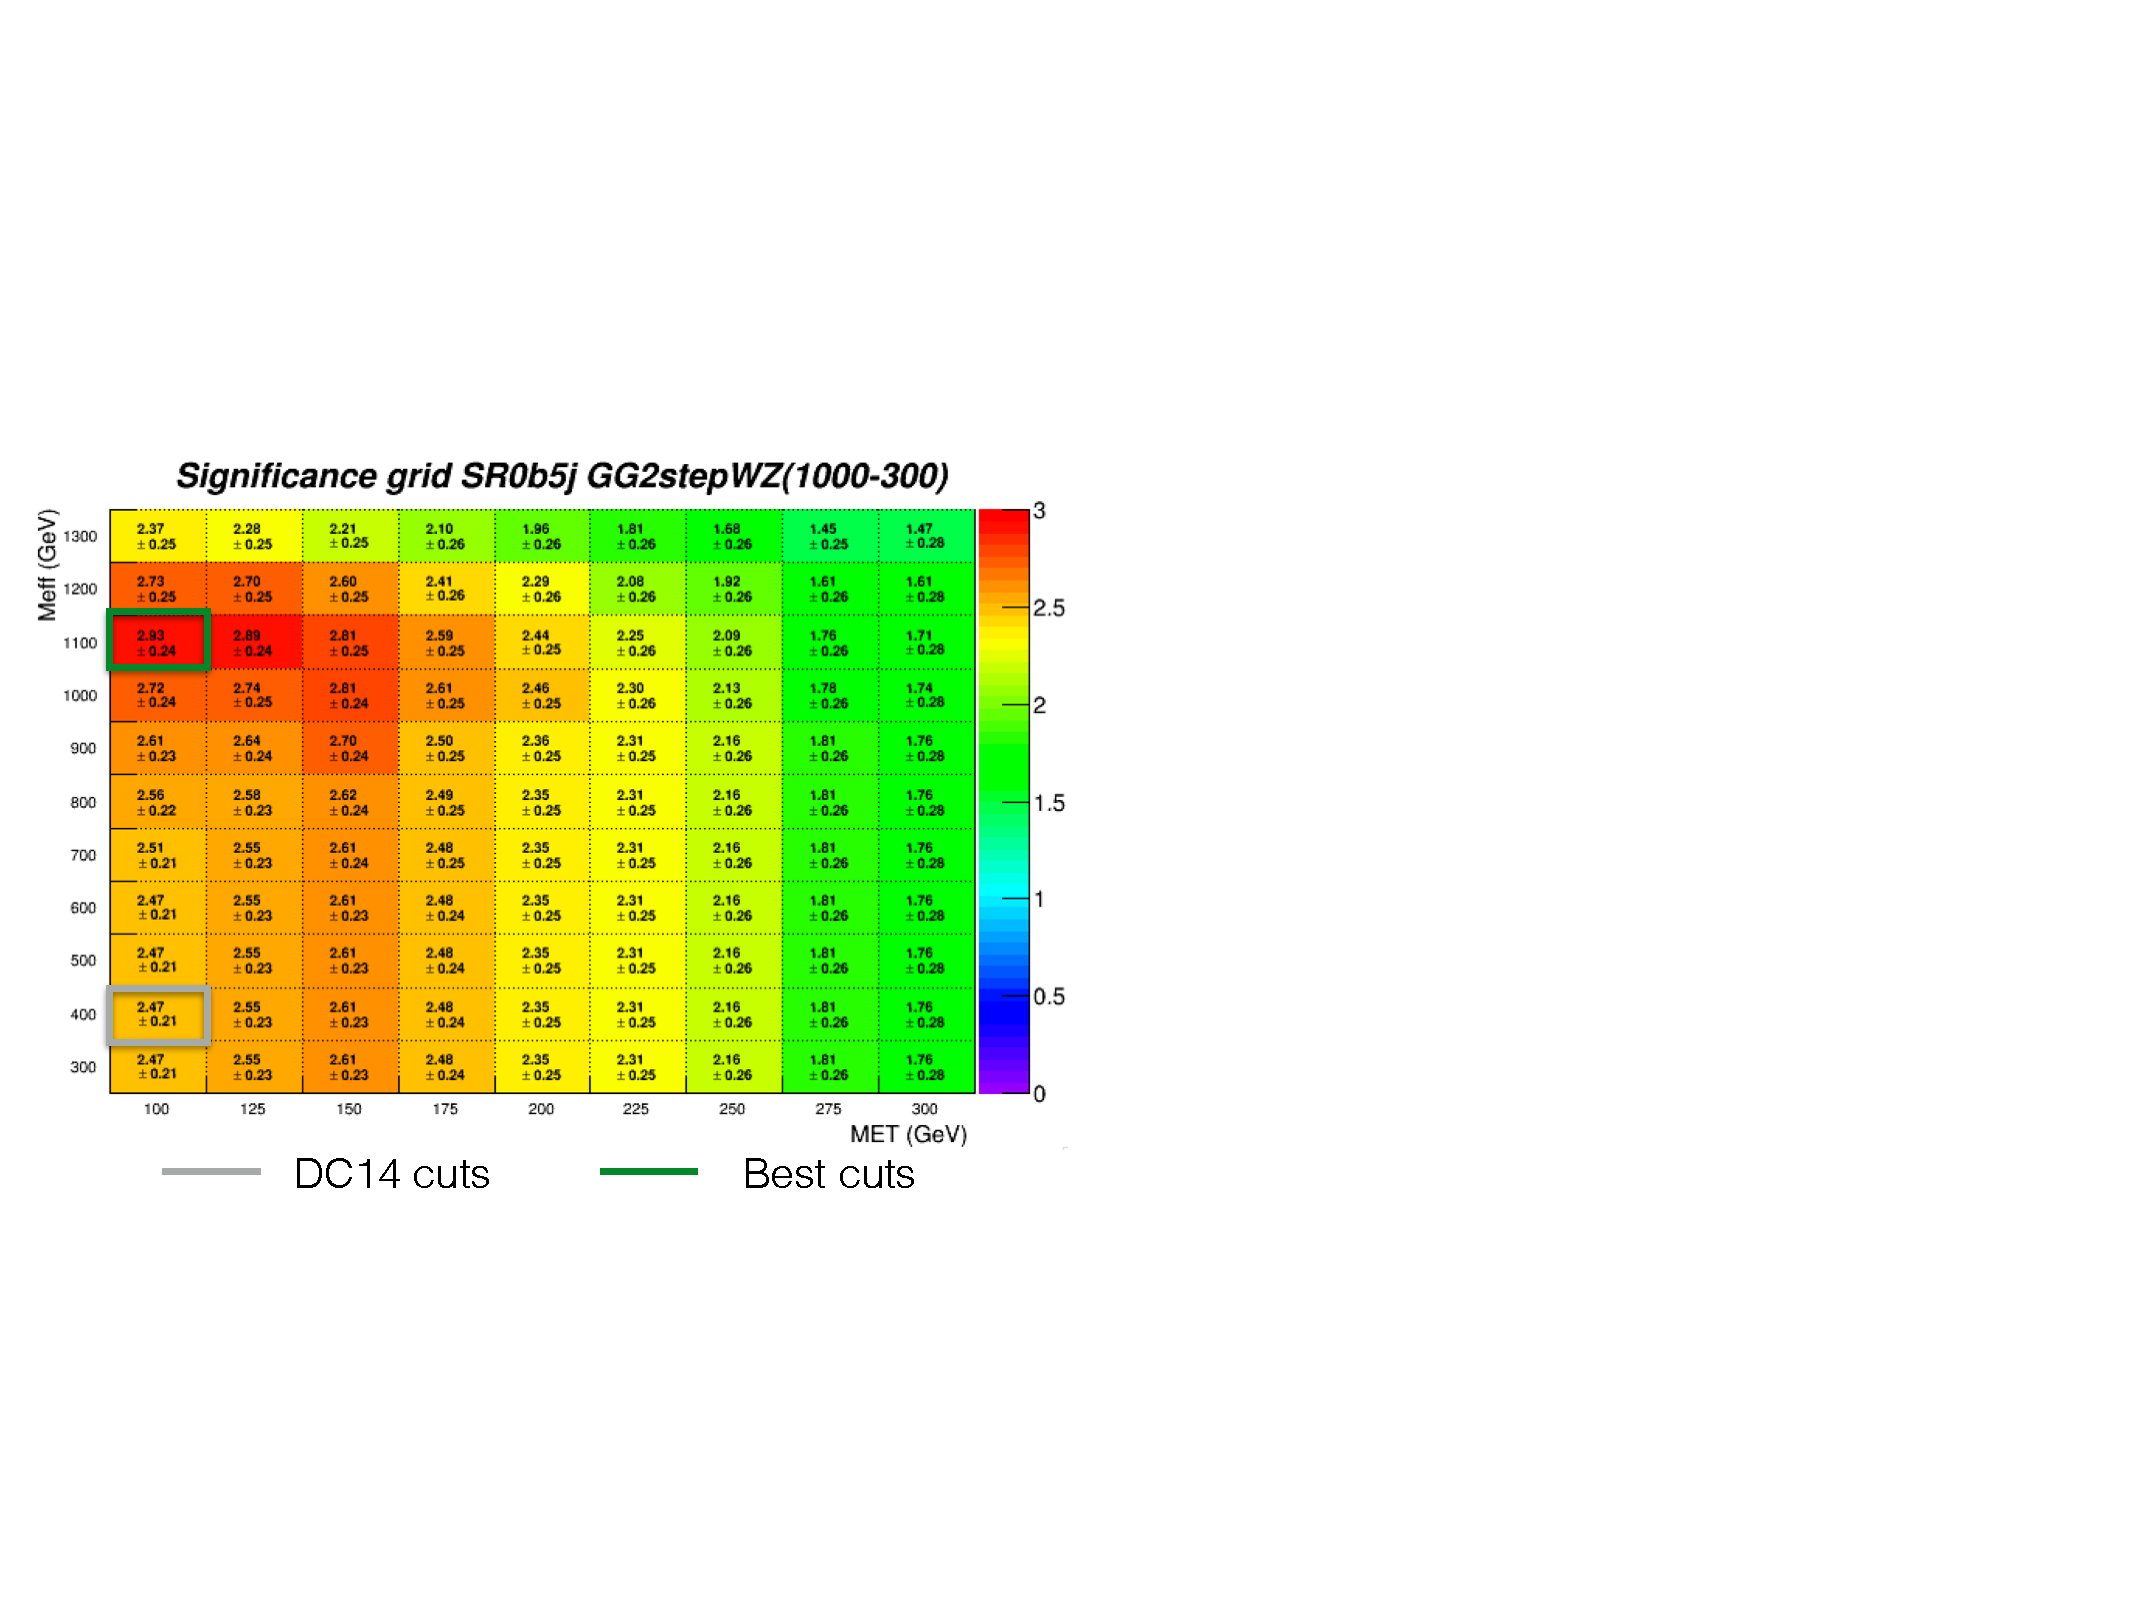
\includegraphics[width=0.49\textwidth]{OPTIMIZATION/Scan1.pdf}
  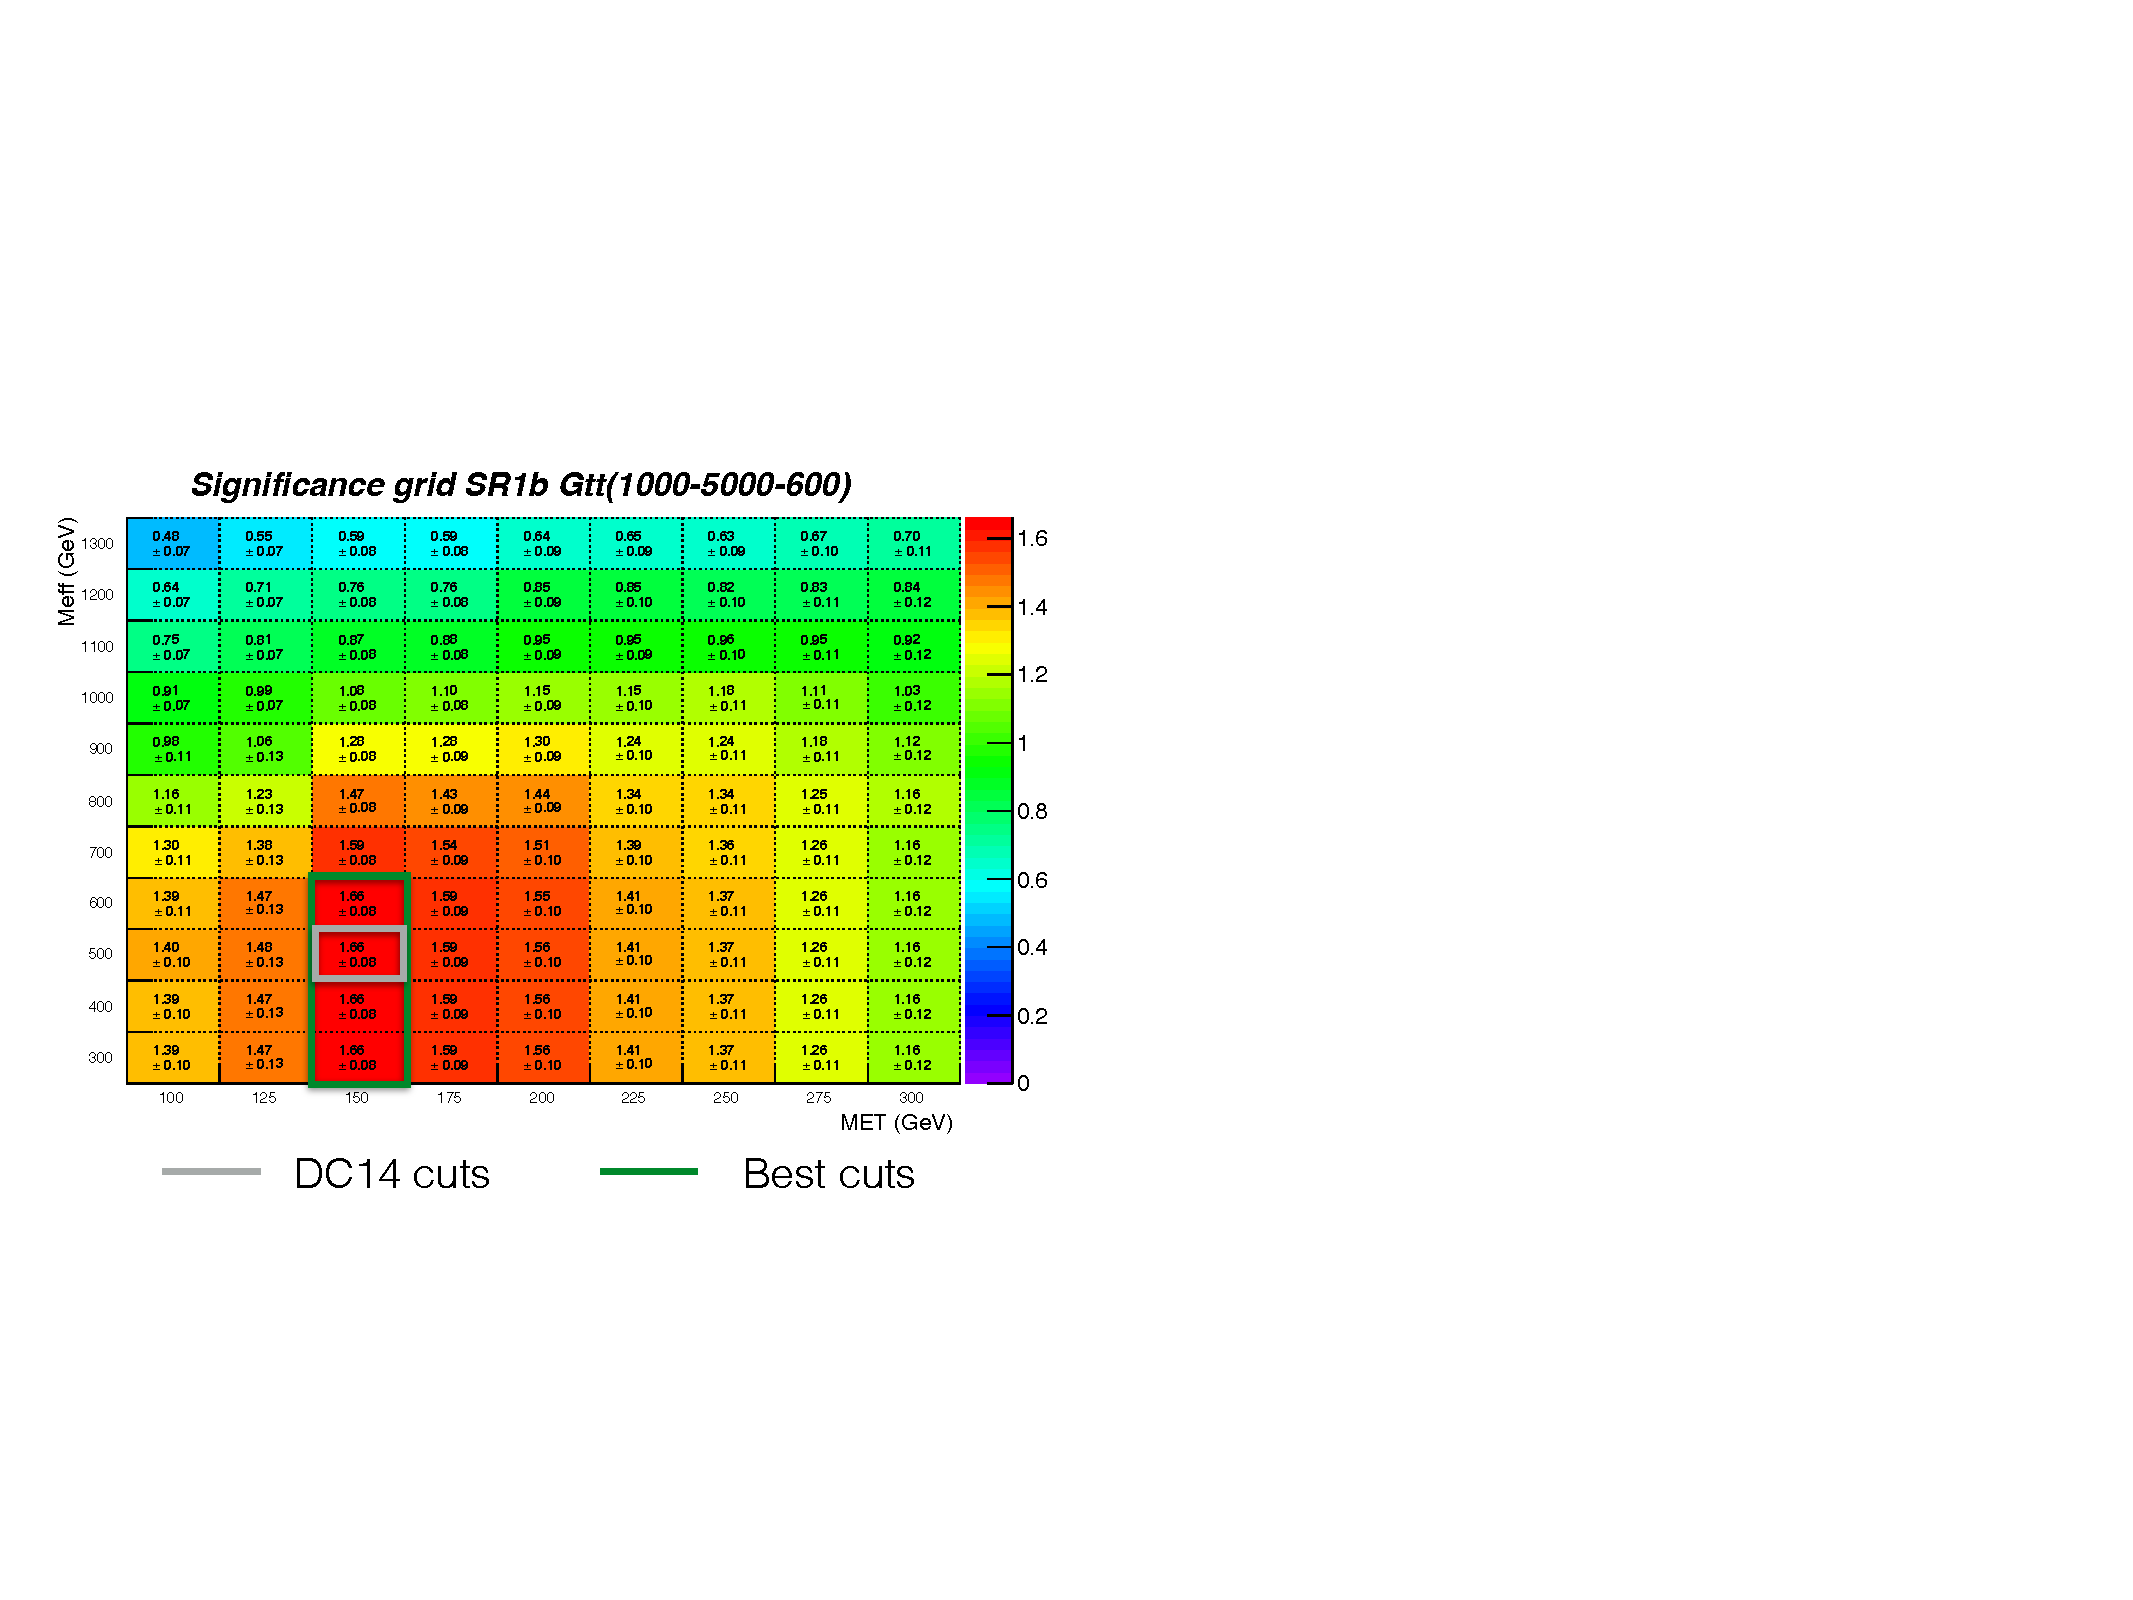
\includegraphics[width=0.49\textwidth]{OPTIMIZATION/Scan2.pdf}
  \caption{Example of (\met, \meff) scans for SR0b5j (left) and SR3b (right). The configurations with maximum significance are highlighted as well as the outcome of the DC14 optimization studies.}
\label{fig:OptimScan}


\end{figure}


%\begin{figure}[!htb]
%\centering
%  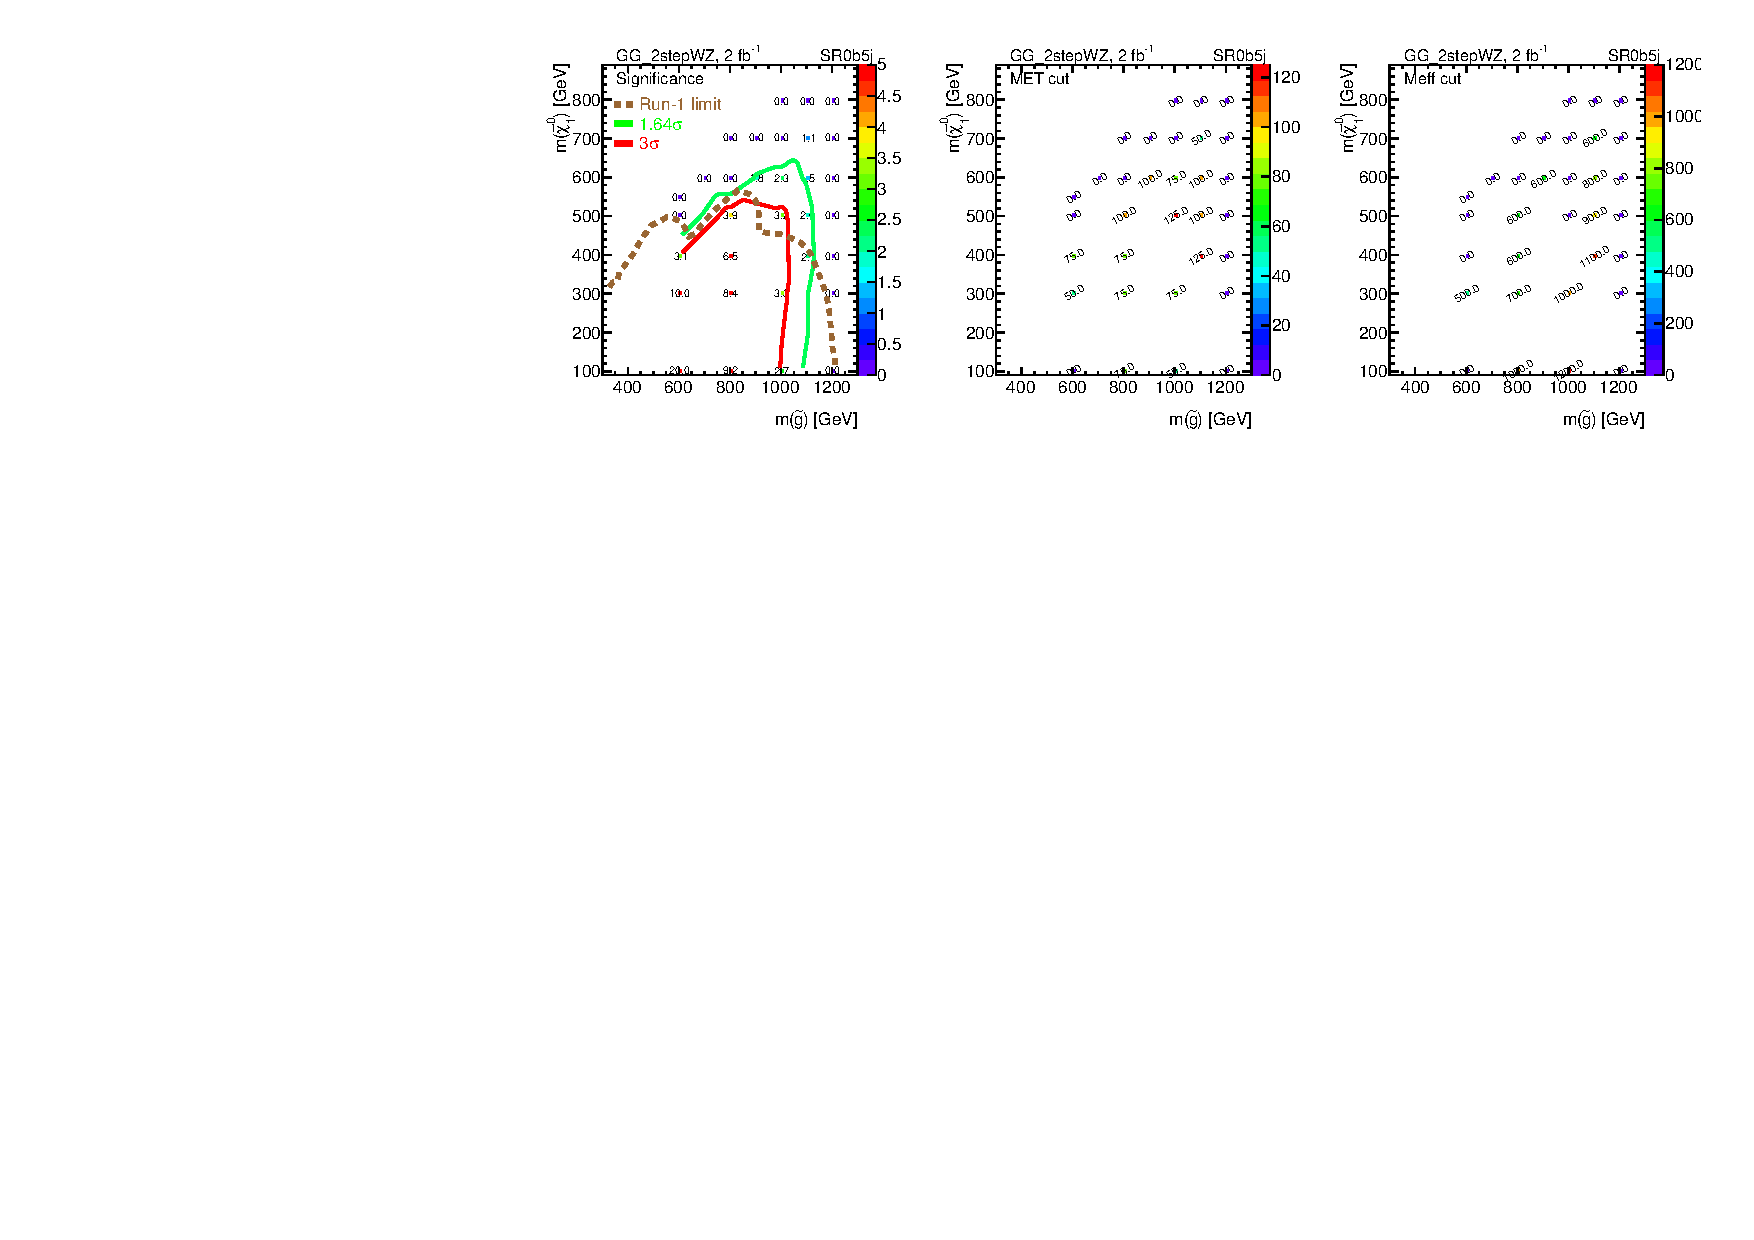
\includegraphics[width=\textwidth]{OPTIMIZATION/Optimiz_SR0b5j_2fb.pdf}
%  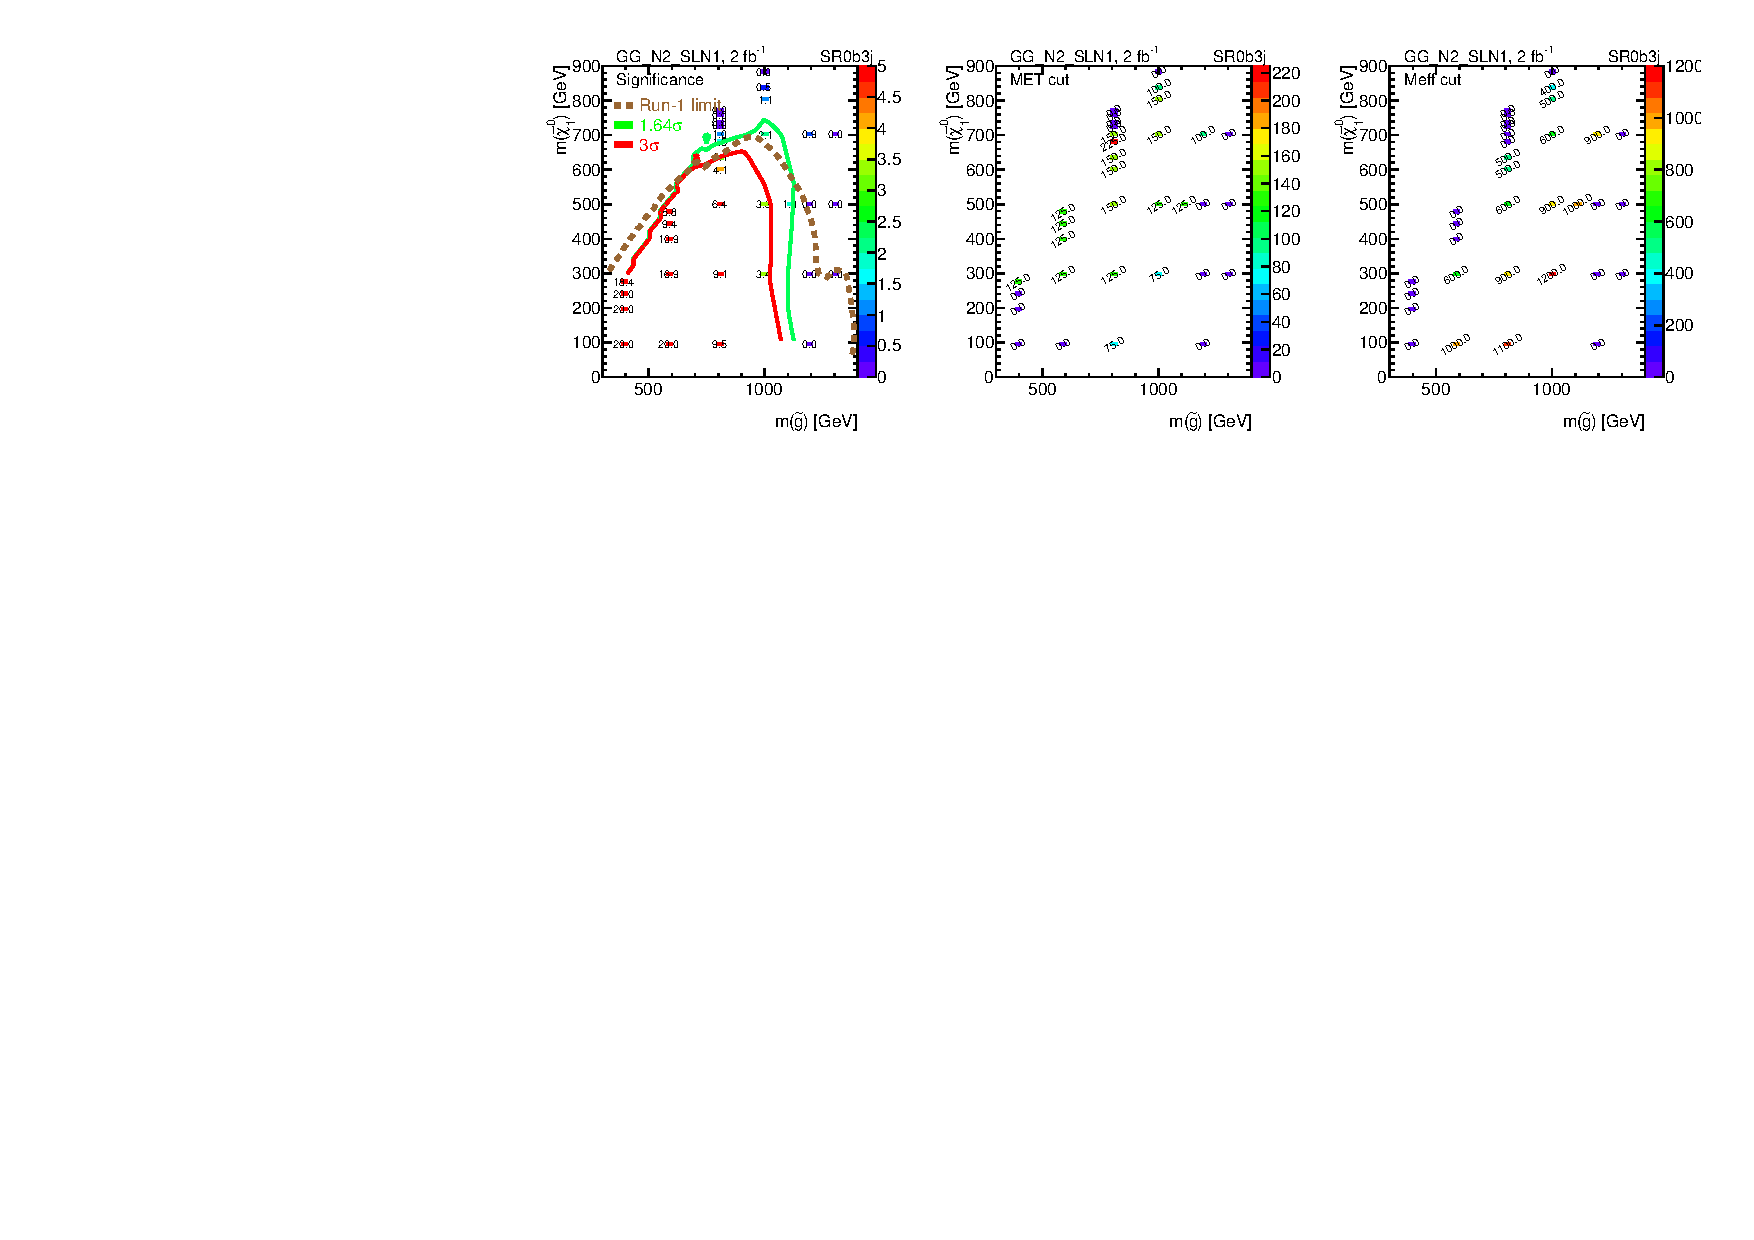
\includegraphics[width=\textwidth]{OPTIMIZATION/Optimiz_SR0b3j_2fb.pdf}
%\caption{Maximum discovery significance (left) for 2~\ifb\, as well as the $\met$ (center) and $\meff$ (right) cuts needed to maximize the significance for SR0b5j in the $\gluino\gluino$ 2-step grid (top) and SR0b3j in the $\gluino\gluino$ 1-step grid (bottom). The Run-1 limits in those models are shown with a brown line.}
%\label{fig:OptimSig2}
%\end{figure}


\subsection{Signal regions}
 
The definition of the exact SR was done as a good compromise across the signal grids shown in 
Figure~\ref{fig:OptimSig1} with a single ($\met$, $\meff$) configuration. 
Tables~\ref{tab:SRdef2}-\ref{tab:SRdef4} show the optimized signal region definitions for scenarios with 2, 3 and 4~\ifb\, respectively. 
The final SR to be used for the 2015 analysis was determined by the luminosity available at the end of the data-taking period: 
if less than 2.5~\ifb\ had been available for analysis after GRL, we would have used the SRs for the 2~\ifb\ scenario; 
if more than 3.5~\ifb\ had been available, we would have used the SRs for the 4~\ifb\ scenario. 
But with the 3.2~\ifb\ eventually collected, we used the definitions corresponding to the intermediate scenario of 3~\ifb.
Figures~\ref{fig:OptimSig2} and \ref{fig:OptimSig4} show the significance values obtained for those signal regions in the SUSY models considered, 
with the 1.64$\sigma$ discovery contours extending beyond the Run-1 exclusions, even achieving a 3$\sigma$ sensitivity in certain regions of the mass parameter space.
 
 
\begin{table}[htb!]
\caption{Signal regions definition for the 2~\ifb\ scenario (to be used for $L <2.5$~fb$^{-1}$). The two leading leptons are required to have \pt~$>$~20~\GeV.}
\hspace{0.5cm}
\label{tab:SRdef2}
\centering
\begin{tabular}{|c|c|c|c|c|c|}
\hline 
\hline
Signal region  &  $N_{\rm{lept}}$   & $N_{b\rm{-jets}}^{20}$    & $N_{\rm{jets}}^{50}$  & \met\ [GeV] & \meff\ [GeV]   \\
\hline\hline
SR3b     &   $\ge$2  &   $\ge$3  &  - & $>$100 & $>$600   \\
\hline
SR1b     &  $\ge$2  &    $\ge$1  &  $\ge$4 &  $>$125 & $>$500 \\
\hline
SR0b5j &  $\ge$2  &    $==$0 &  $\ge$5 &  $>$100 & $>$600 \\
\hline
SR0b3j &  $\ge$3  &    $==$0 &  $\ge$3 &  $>$150 & $>$500 \\
\hline\hline
\end{tabular}
\end{table}

\begin{table}[htb!]
\caption{Signal regions definition for the 3~\ifb\ scenario (to be used for $2.5 \leq L <3.5$~fb$^{-1}$), 
the one eventually used in this analysis. The two leading leptons are required to have \pt~$>$~20~\GeV.}
\hspace{0.5cm}
\label{tab:SRdef3}
\centering
\begin{tabular}{|c|c|c|c|c|c|}
\hline 
\hline
Signal region  &  $N_{\rm{lept}}$   & $N_{b\rm{-jets}}^{20}$    & $N_{\rm{jets}}^{50}$  & \met\ [GeV] & \meff\ [GeV]   \\
\hline\hline
SR3b     &   $\ge$2  &   $\ge$3  &  - & $>$125 & $>$650   \\
\hline
SR1b     &  $\ge$2  &    $\ge$1  &  $\ge$4 &  $>$150 & $>$550 \\
\hline
SR0b5j &  $\ge$2  &    $==$0 &  $\ge$5 &  $>$125 & $>$650 \\
\hline
SR0b3j &  $\ge$3  &    $==$0 &  $\ge$3 &  $>$200 & $>$550 \\
\hline\hline
\end{tabular}
\end{table}

\begin{table}[htb!]
\caption{Signal regions definition for the 4~\ifb\ scenario (to be used for $L \geq 3.5$~fb$^{-1}$). The two leading leptons are required to have \pt~$>$~20~\GeV.}
\hspace{0.5cm}
\label{tab:SRdef4}
\centering
\begin{tabular}{|c|c|c|c|c|c|}
\hline 
\hline
Signal region  &  $N_{\rm{lept}}$   & $N_{b\rm{-jets}}^{20}$    & $N_{\rm{jets}}^{50}$  & \met\ [GeV] & \meff\ [GeV]   \\
\hline\hline
SR3b     &   $\ge$2  &   $\ge$3  &  - & $>$125 & $>$700   \\
\hline
SR1b     &  $\ge$2  &    $\ge$1  &  $\ge$4 &  $>$150 & $>$600 \\
\hline
SR0b5j &  $\ge$2  &    $==$0 &  $\ge$5 &  $>$125 & $>$700 \\
\hline
SR0b3j &  $\ge$3  &    $==$0 &  $\ge$3 &  $>$200 & $>$600 \\
\hline\hline
\end{tabular}
\end{table}

\begin{figure}[!htb]
\centering
  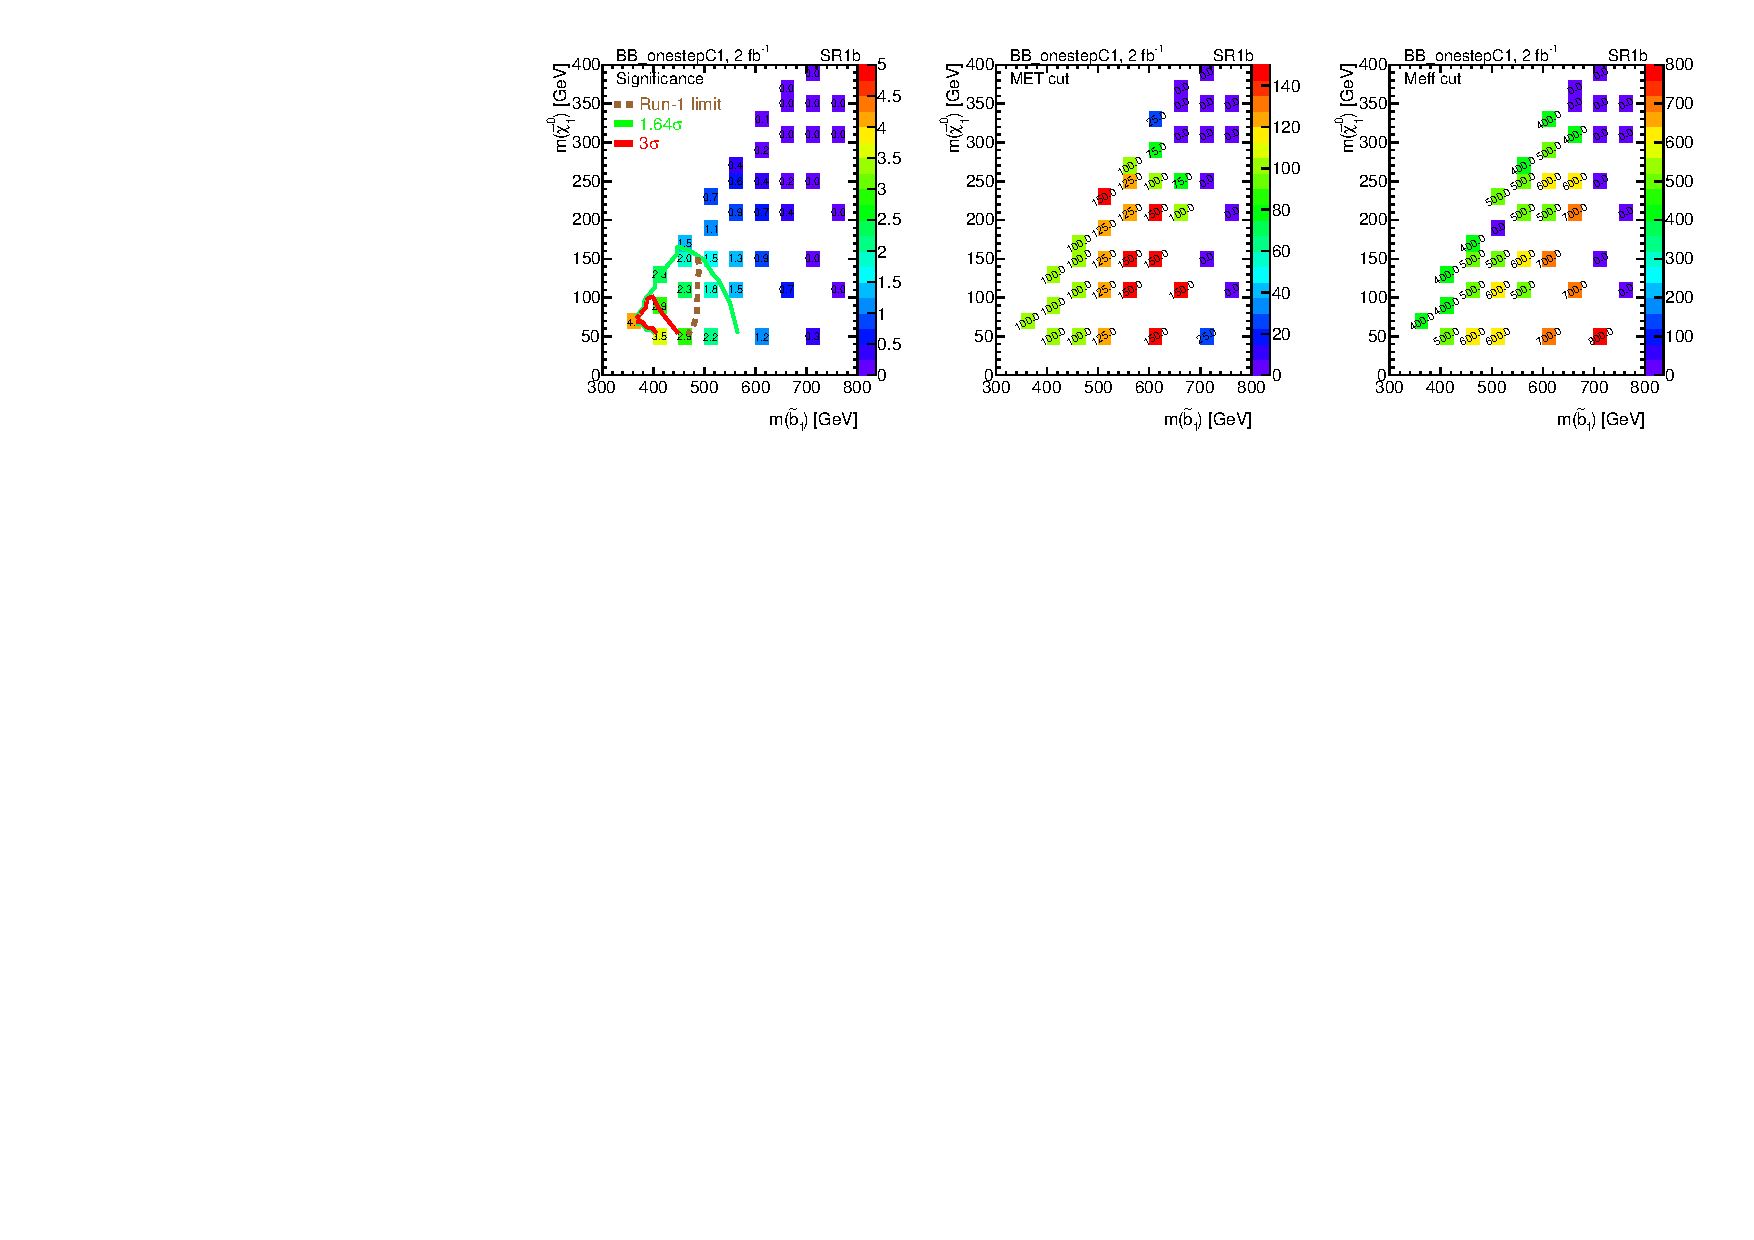
\includegraphics[width=0.9\textwidth]{OPTIMIZATION/Optimiz_SR1b_2fb.pdf}
  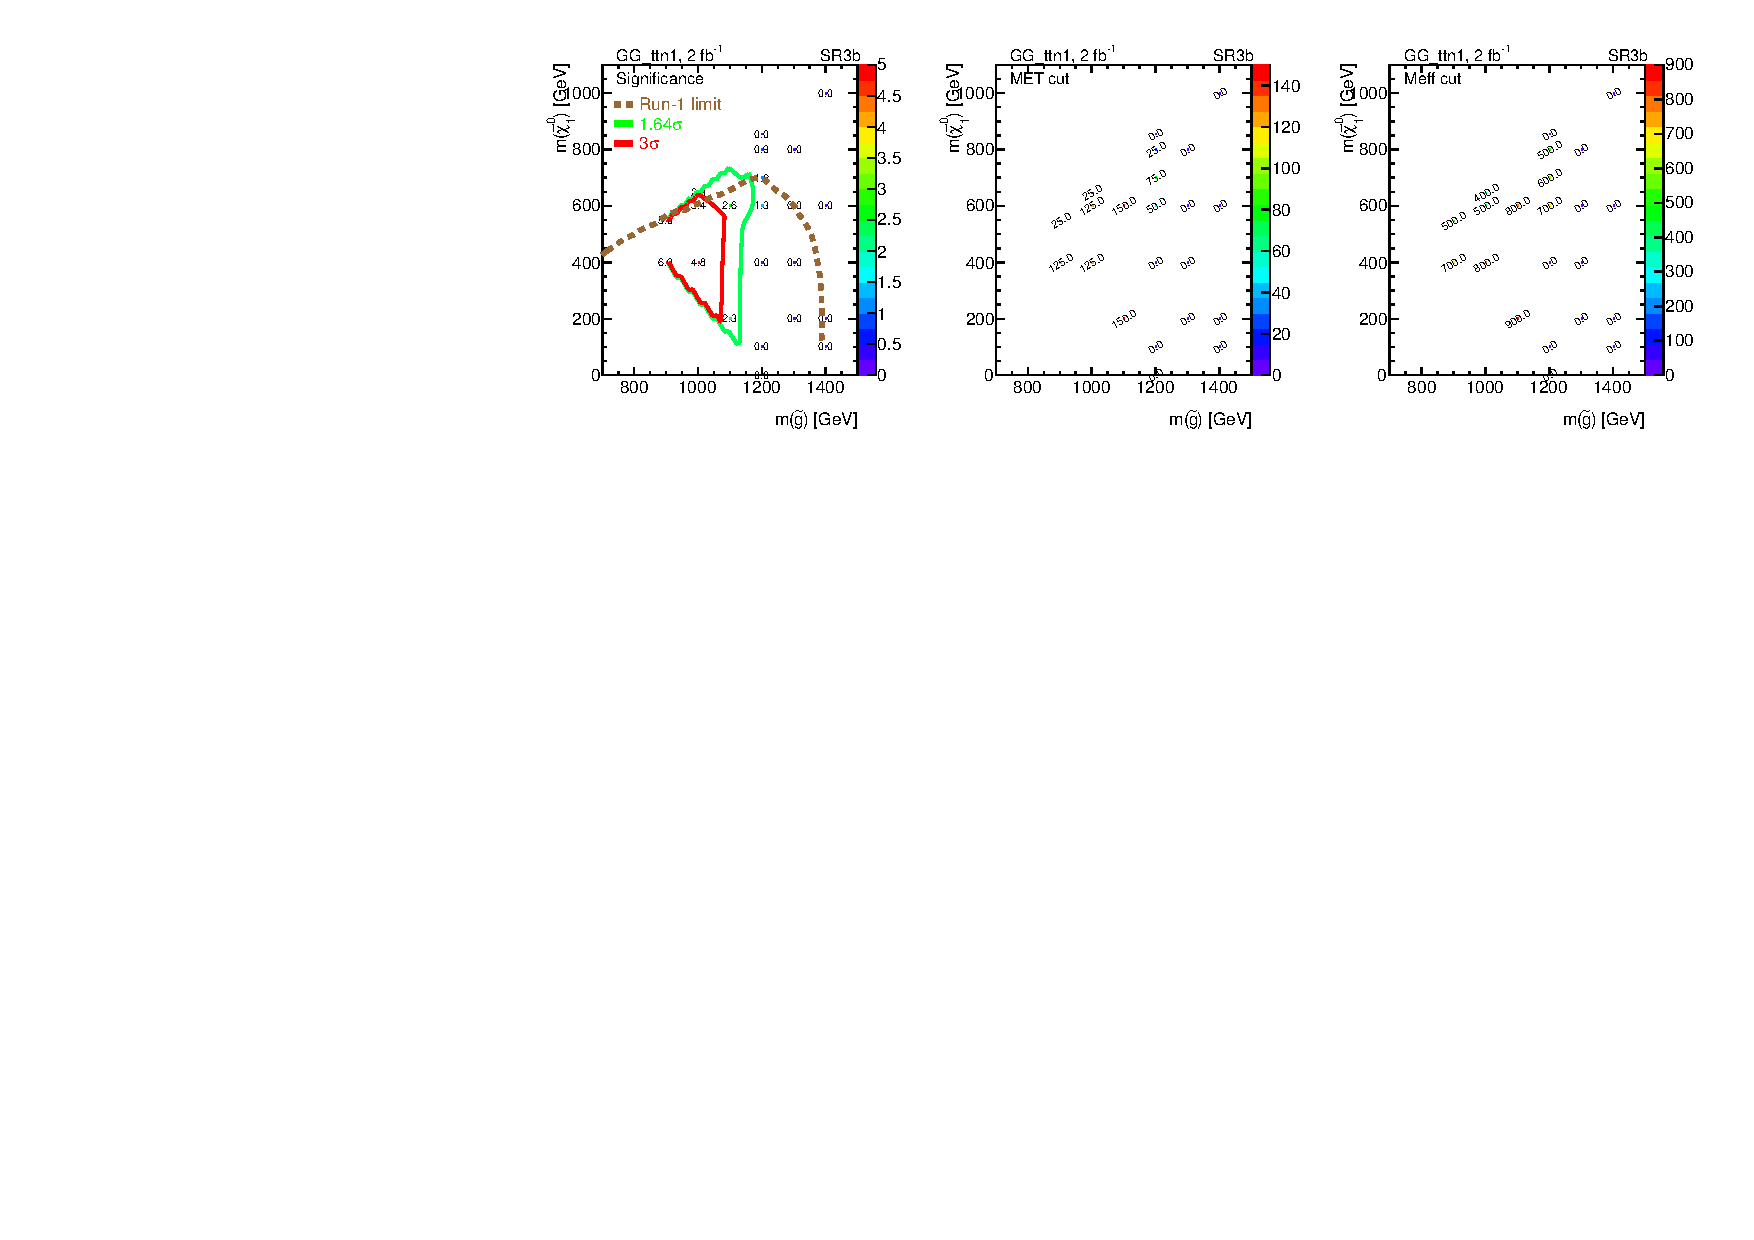
\includegraphics[width=0.9\textwidth]{OPTIMIZATION/Optimiz_SR3b_2fb.pdf}
  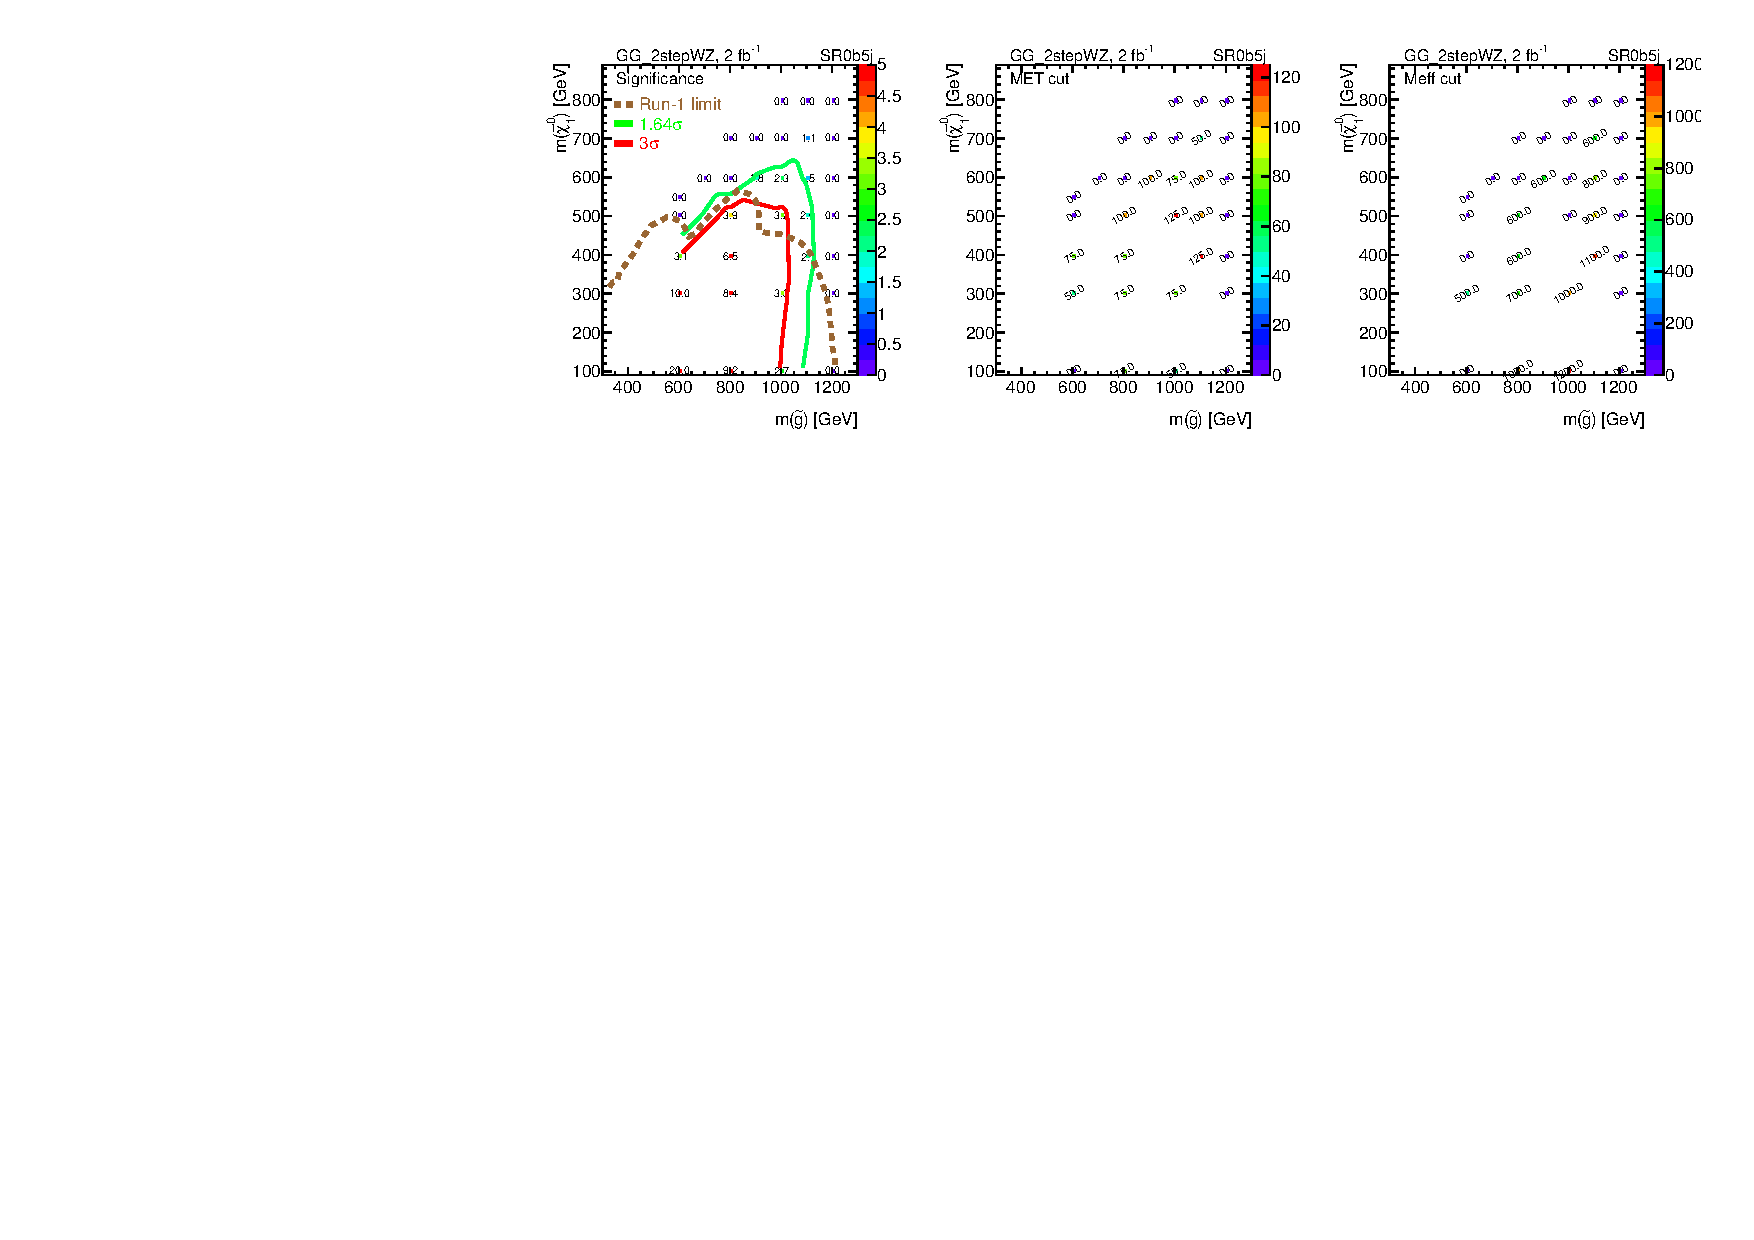
\includegraphics[width=0.9\textwidth]{OPTIMIZATION/Optimiz_SR0b5j_2fb.pdf}
  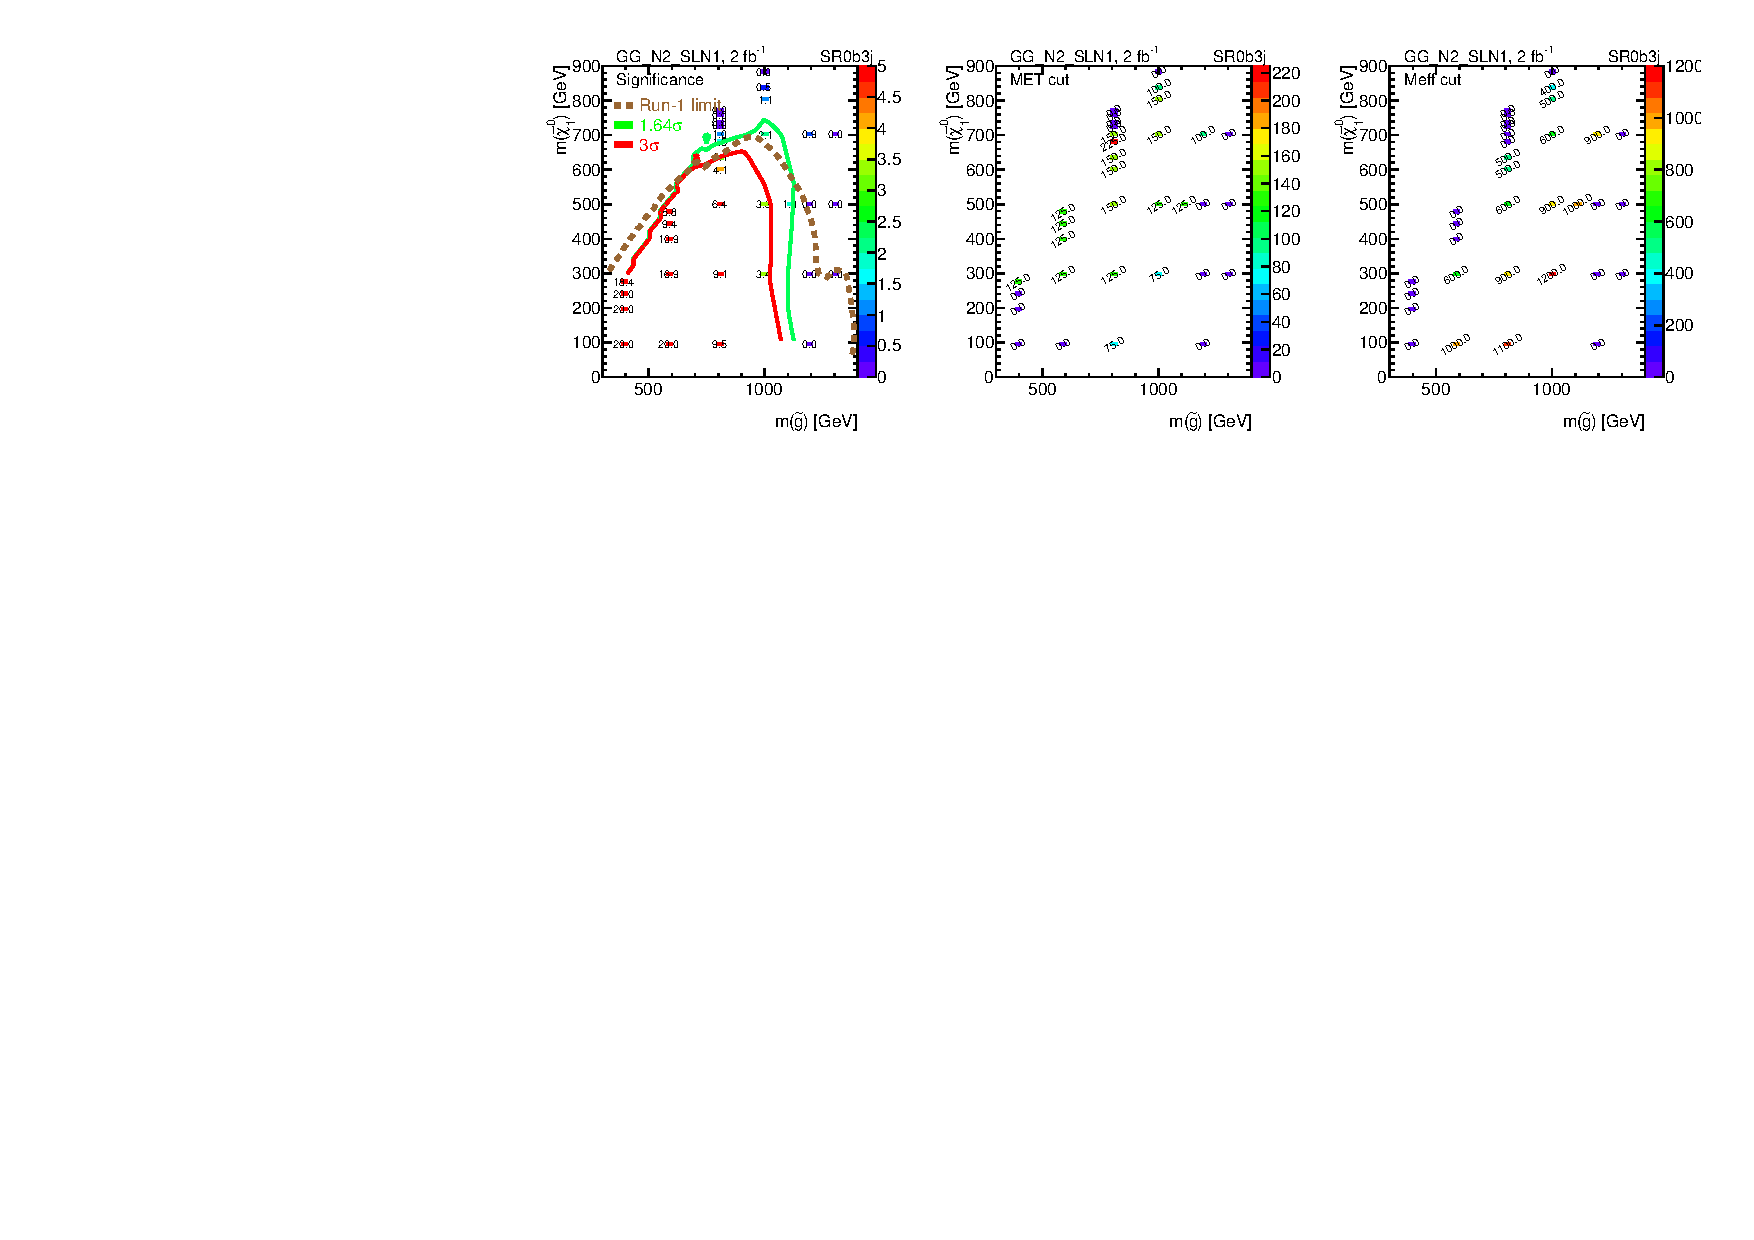
\includegraphics[width=0.9\textwidth]{OPTIMIZATION/Optimiz_SR0b3j_2fb.pdf}
  \caption{Maximum discovery significance (left) for 2~\ifb, as well as the $\met$ (center) and $\meff$ (right) cuts needed to maximize the significance for: (from top to bottom) SR1b in the $\sbot\sbot^*\to t\bar t\tilde\chi_1^+\tilde\chi_1^-$ grid, SR3b in the $\gluino\gluino\to t\bar tt\bar t\ninoone\ninoone$ grid, SR0b5j in the $\gluino\gluino$ with $\gluino\to q\bar{q}'WZ\ninoone$ grid and SR0b3j in the $\gluino\gluino$ with $\gluino\to q\bar{q}(\ell\ell/\ell\nu)\ninoone$ grid. The Run-1 limits in those models are shown with a brown line, and the 1.64$\sigma$ and 3$\sigma$ discovery contours from the proposed signal regions are shown in green and red, respectively.}
\label{fig:OptimSig1}
\end{figure}



\begin{figure}[!htb]
\centering
  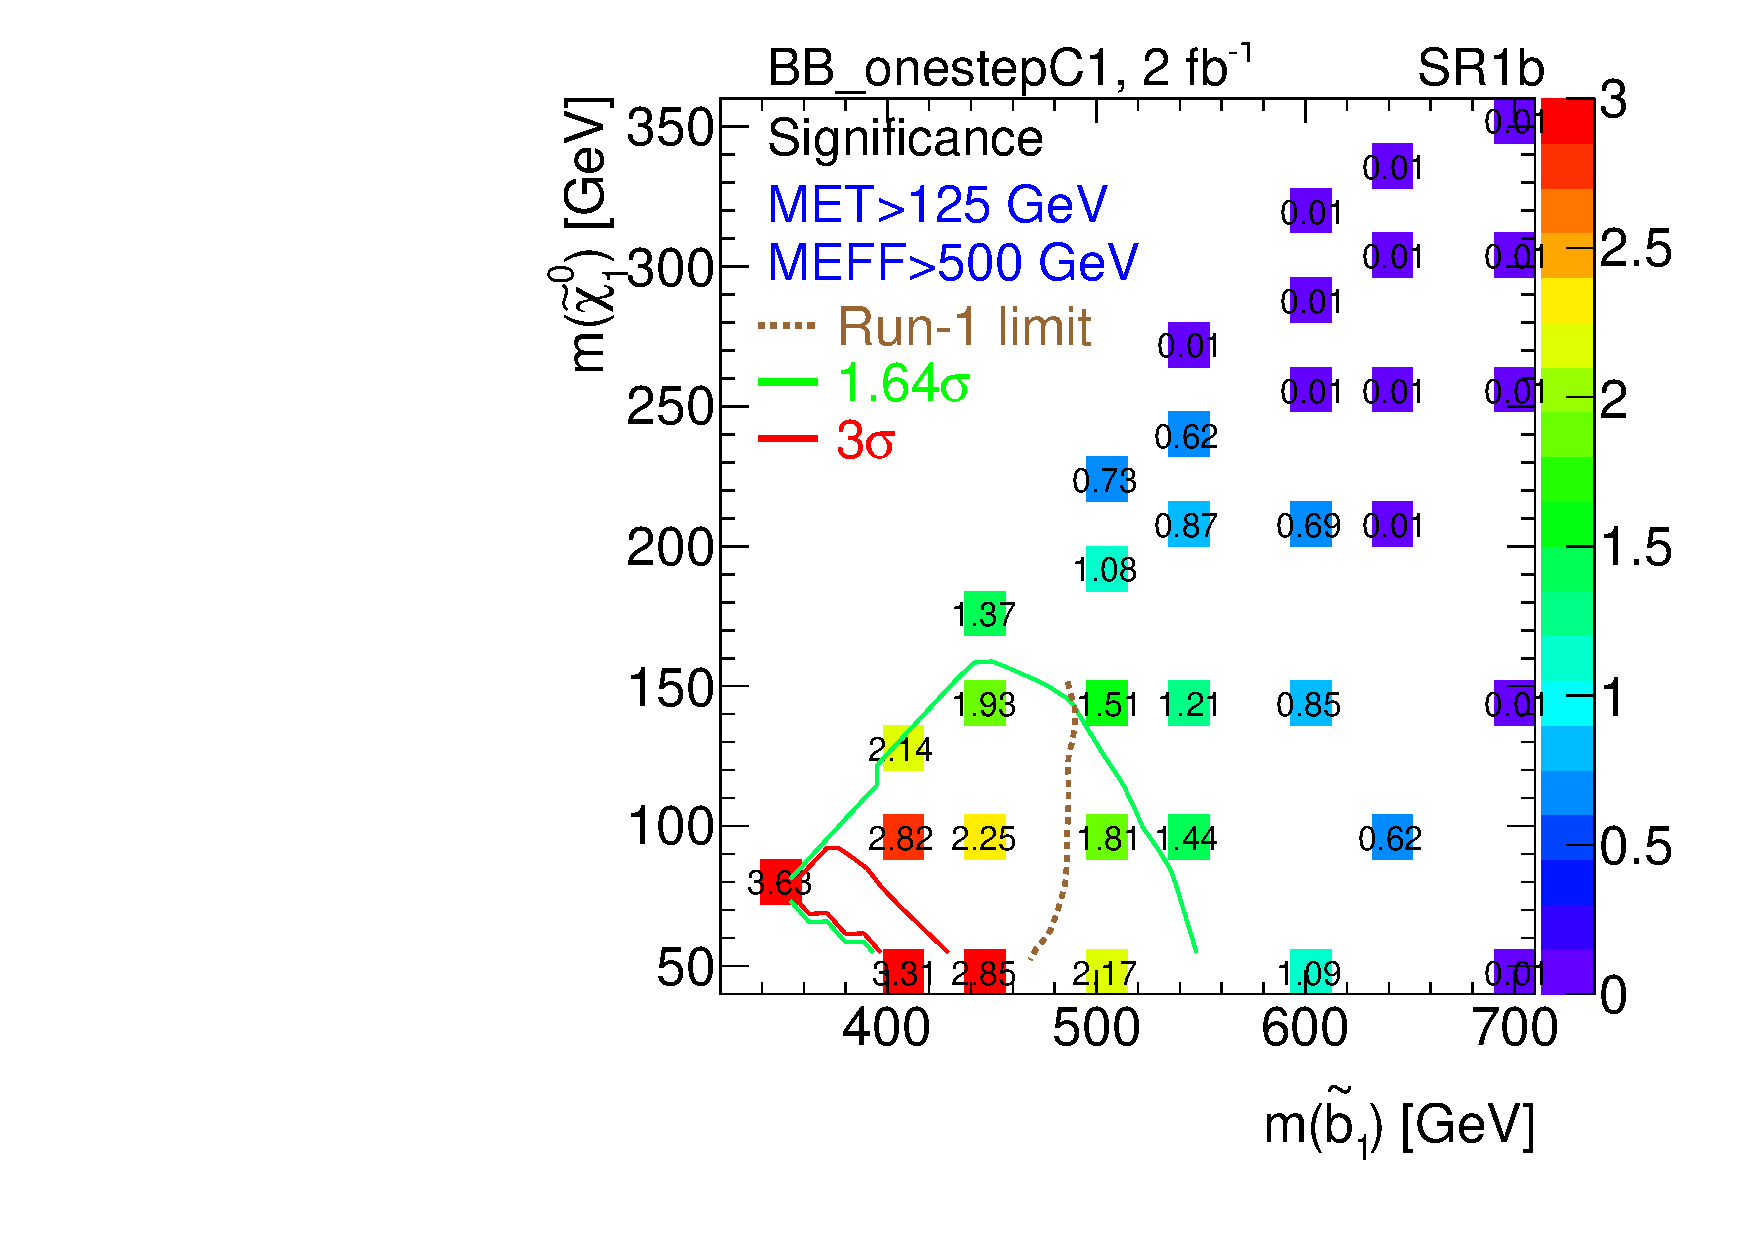
\includegraphics[width=0.4\textwidth]{OPTIMIZATION/Optimiz_SR1b_2fb_125_500.pdf}
  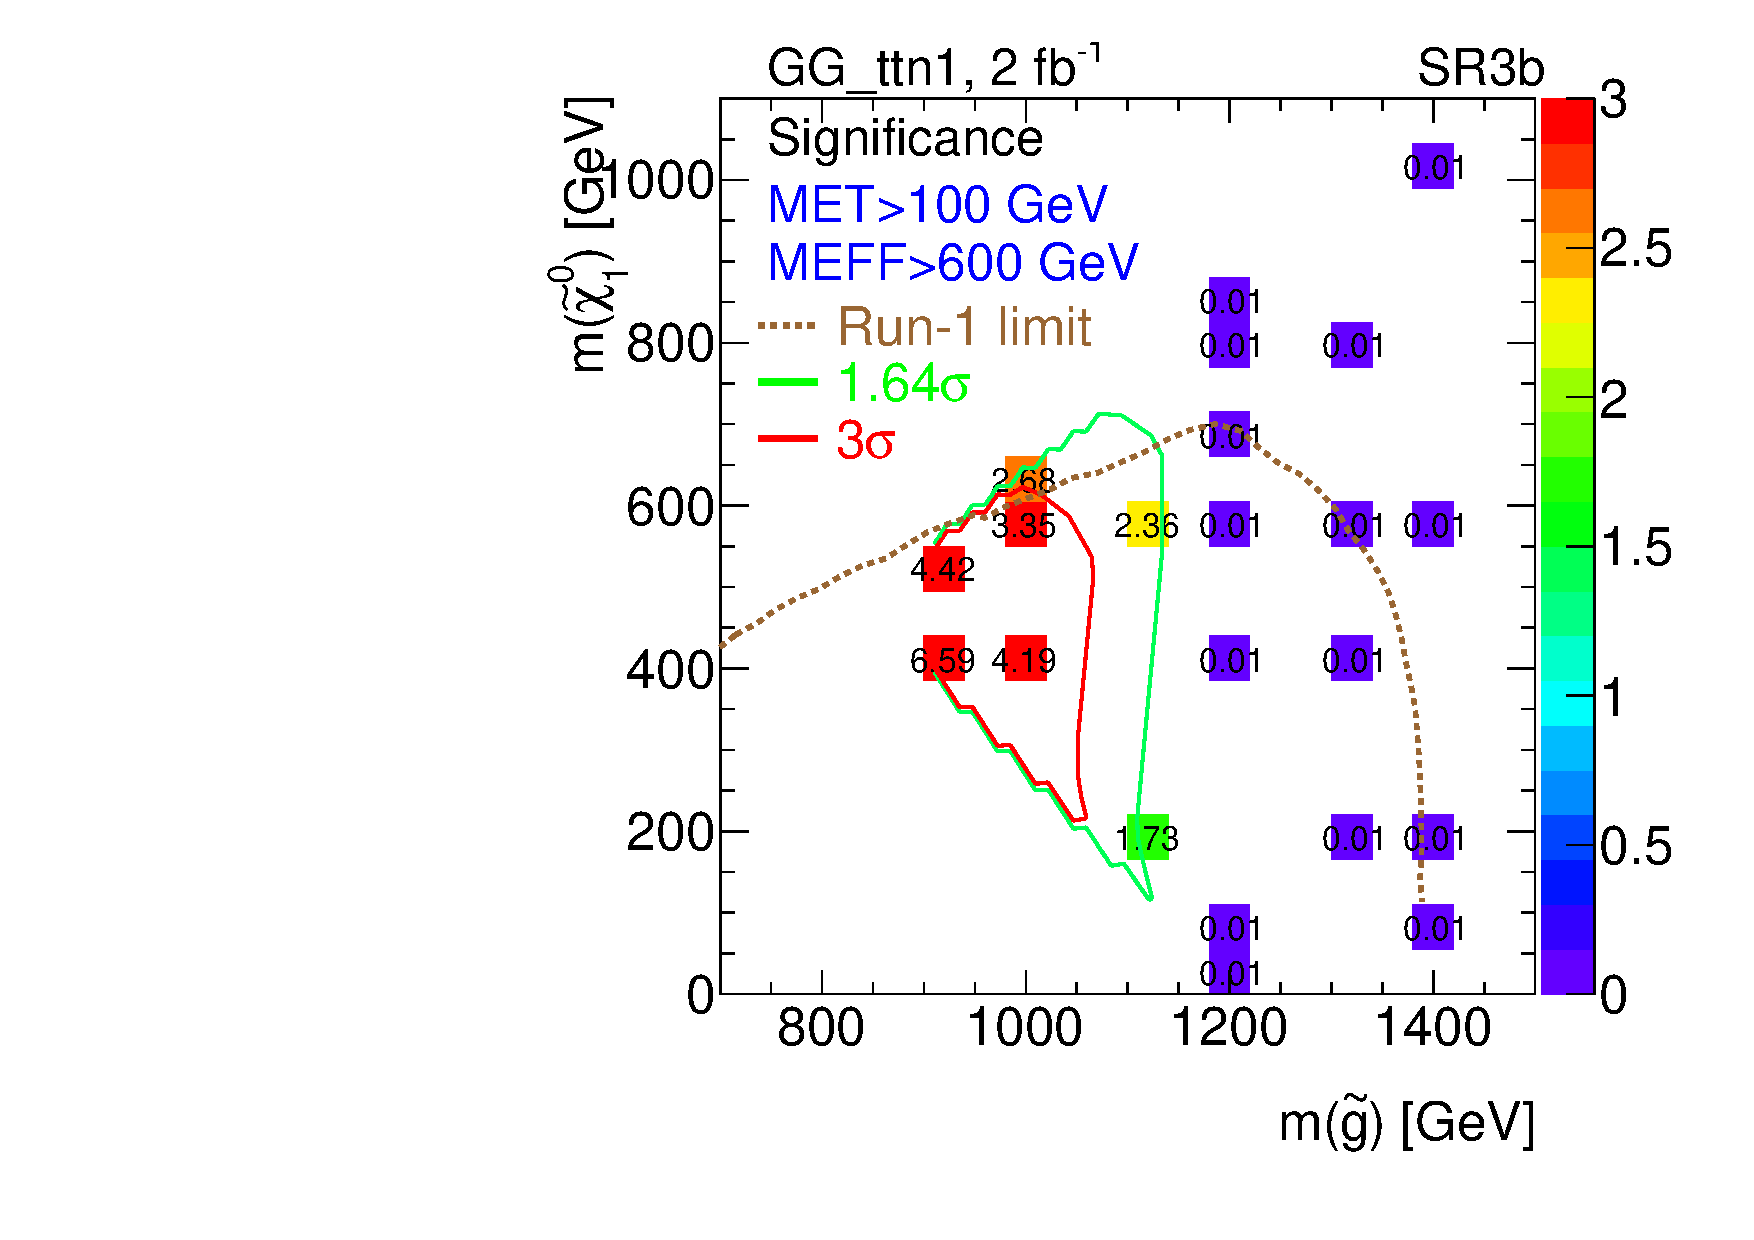
\includegraphics[width=0.4\textwidth]{OPTIMIZATION/Optimiz_SR3b_2fb_100_600.pdf}\\
  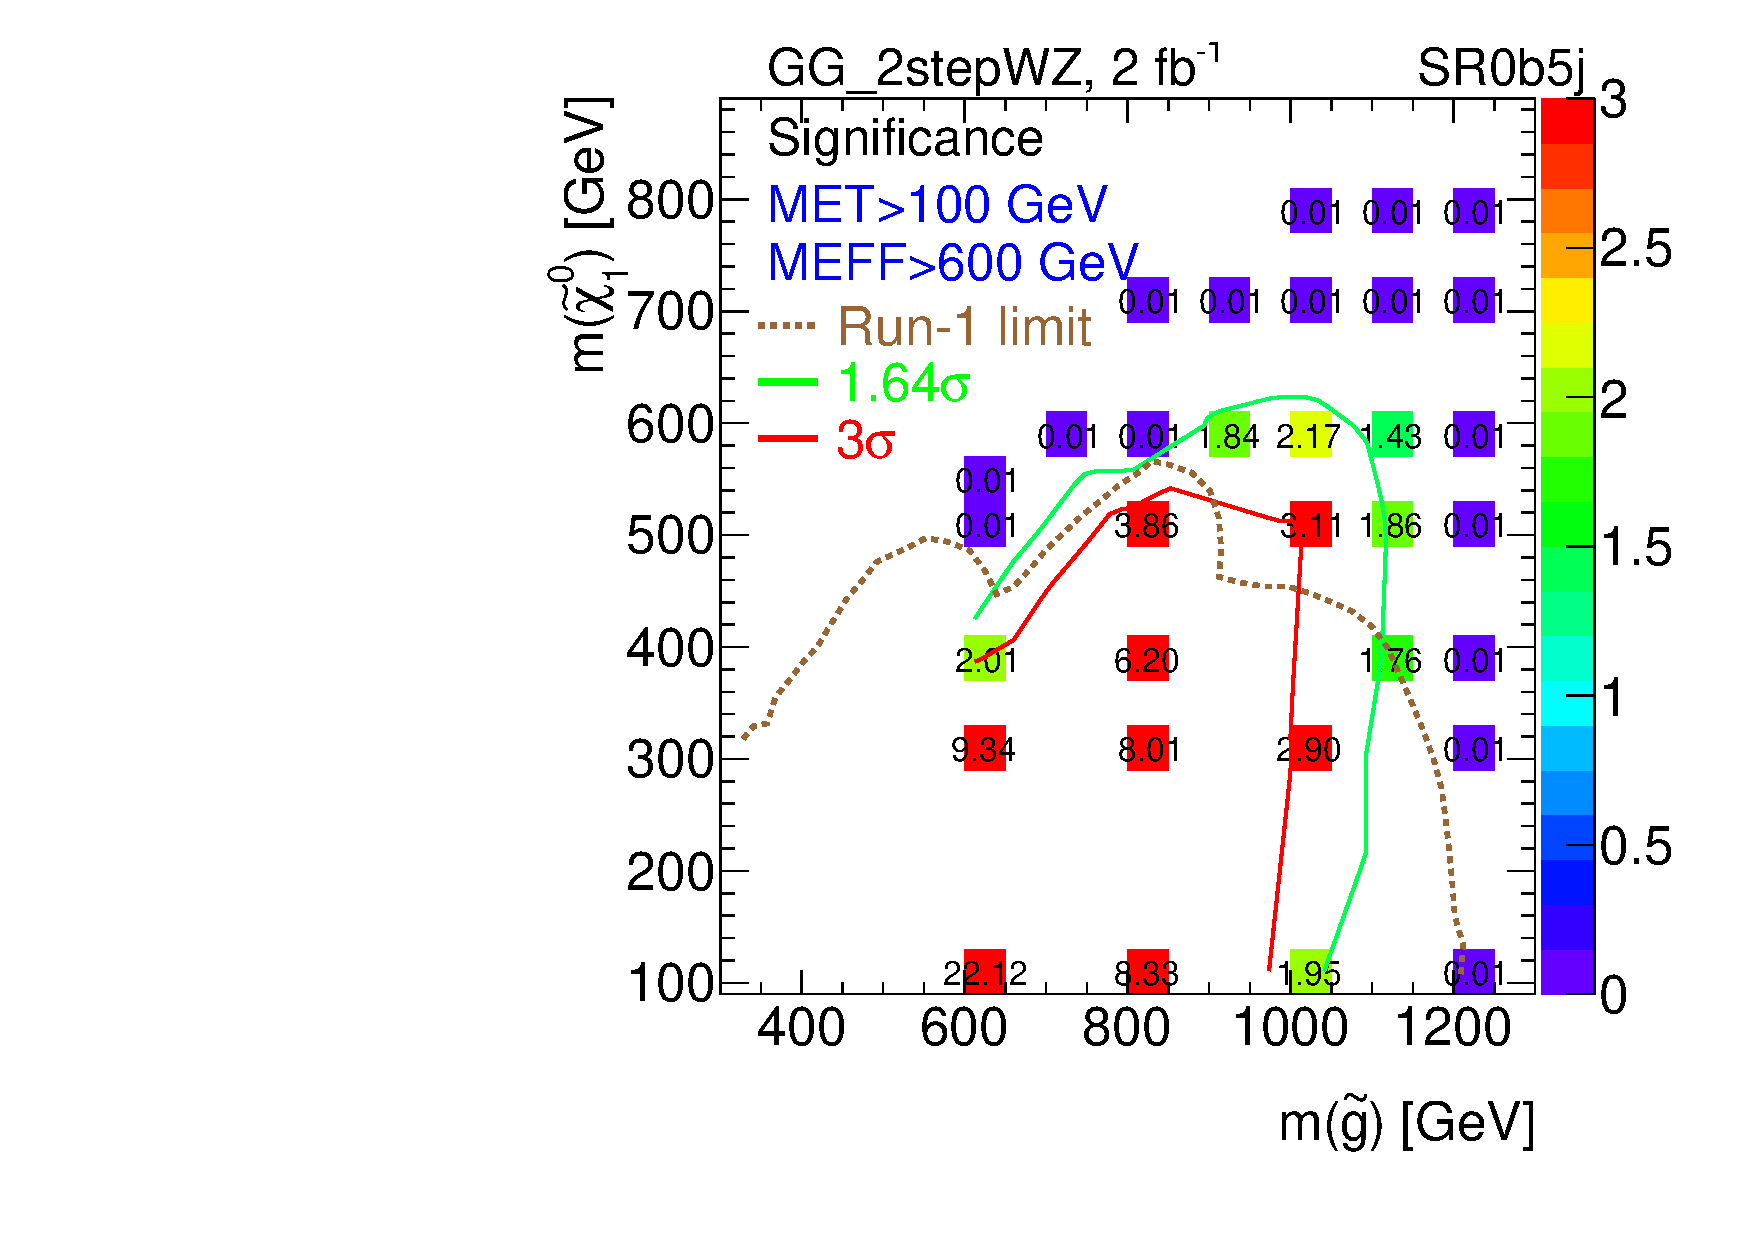
\includegraphics[width=0.4\textwidth]{OPTIMIZATION/Optimiz_SR0b5j_2fb_100_600.pdf}
  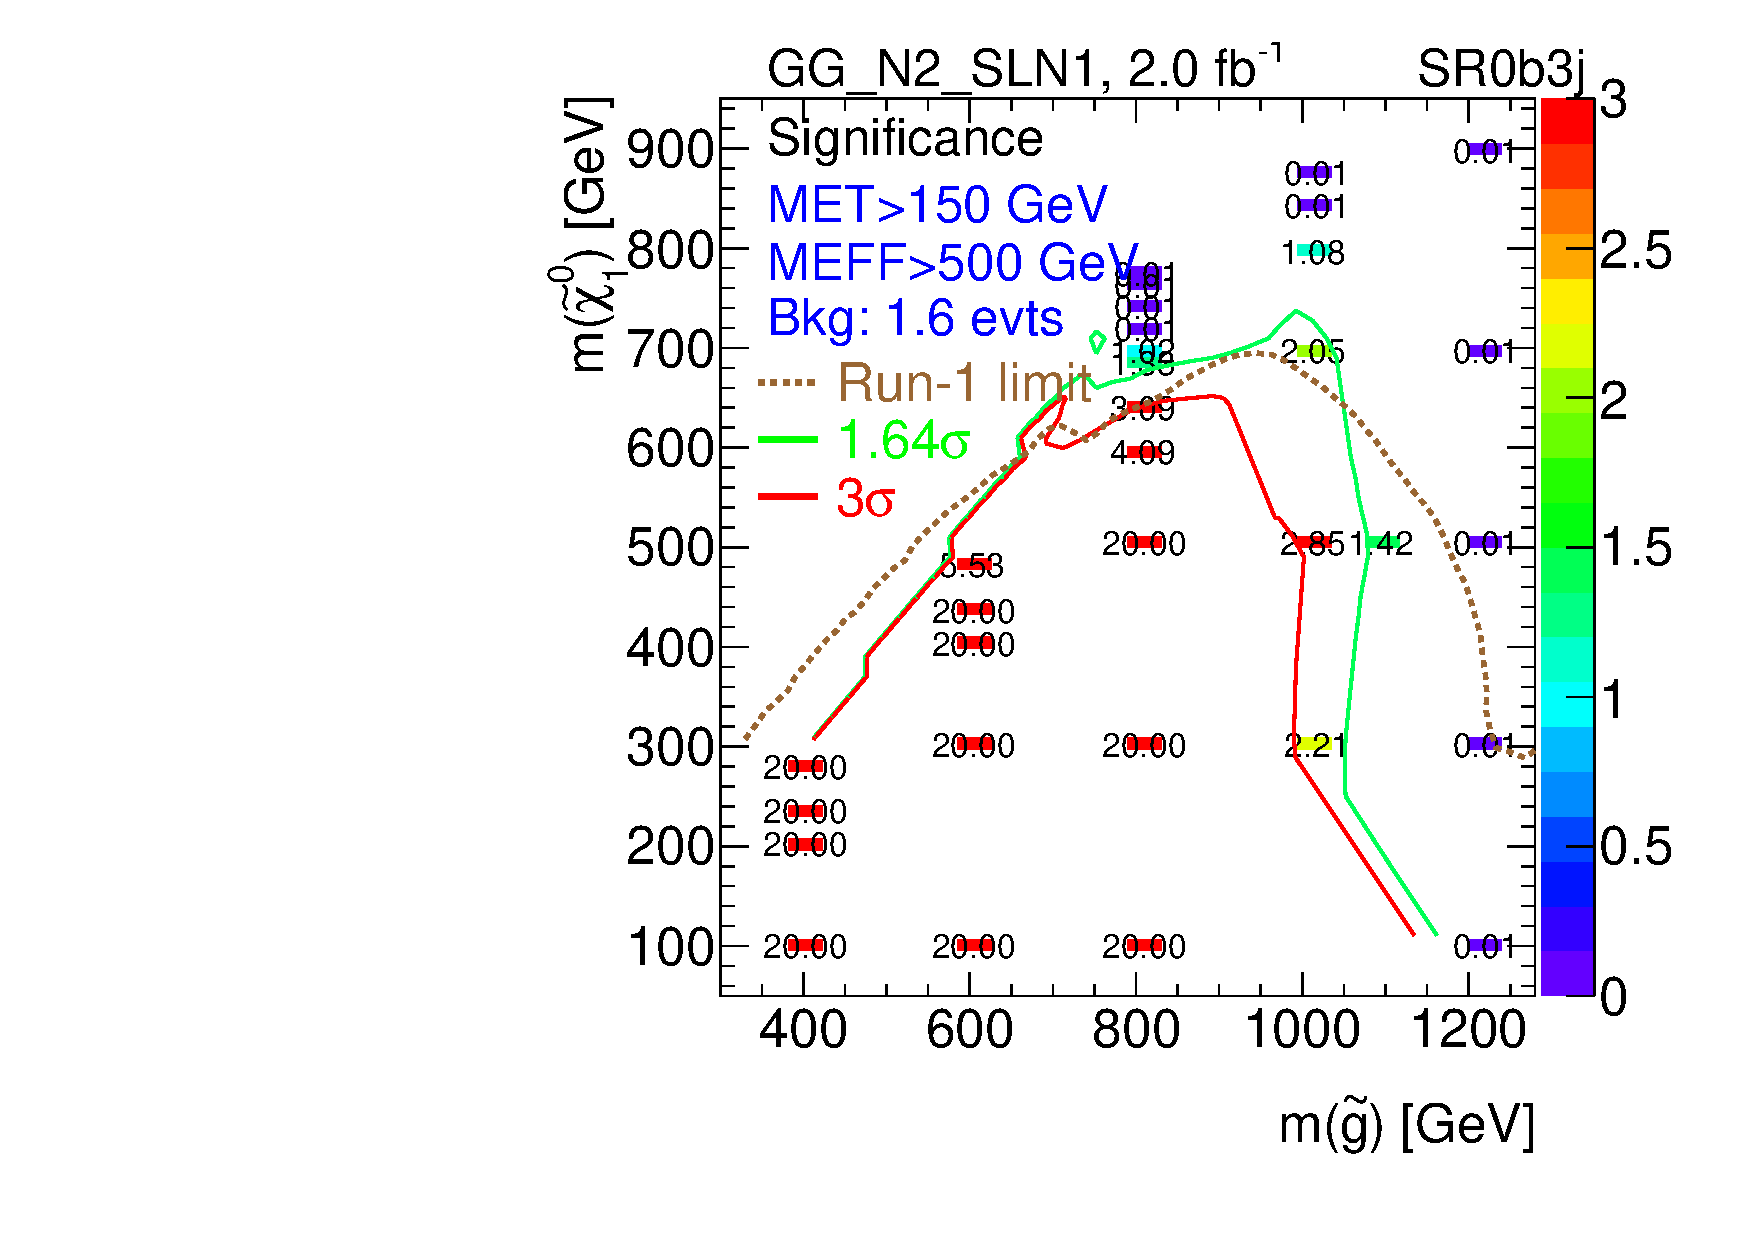
\includegraphics[width=0.4\textwidth]{OPTIMIZATION/Optimiz_SR0b3j_2fb_150_500.pdf}
  \caption{Discovery significance for the SRs defined in Table~\ref{tab:SRdef2} (2~\ifb) for SR1b in the $\sbot\sbot^*\to t\bar t\tilde\chi_1^+\tilde\chi_1^-$ grid (top left), SR3b in the $\gluino\gluino\to t\bar tt\bar t\ninoone\ninoone$ grid (top right), SR0b5j in the $\gluino\gluino$ with $\gluino\to q\bar{q}'WZ\ninoone$ grid (bottom left) and SR0b3j in the $\gluino\gluino$ with $\gluino\to q\bar{q}(\ell\ell/\ell\nu)\ninoone$ grid (bottom right). The Run-1 limits in those models are shown with a brown line, and the 1.64$\sigma$ and 3$\sigma$ discovery contours from the proposed signal regions are shown in green and red, respectively.}
\label{fig:OptimSig2}
\end{figure}


\begin{figure}[!htb]
\centering
  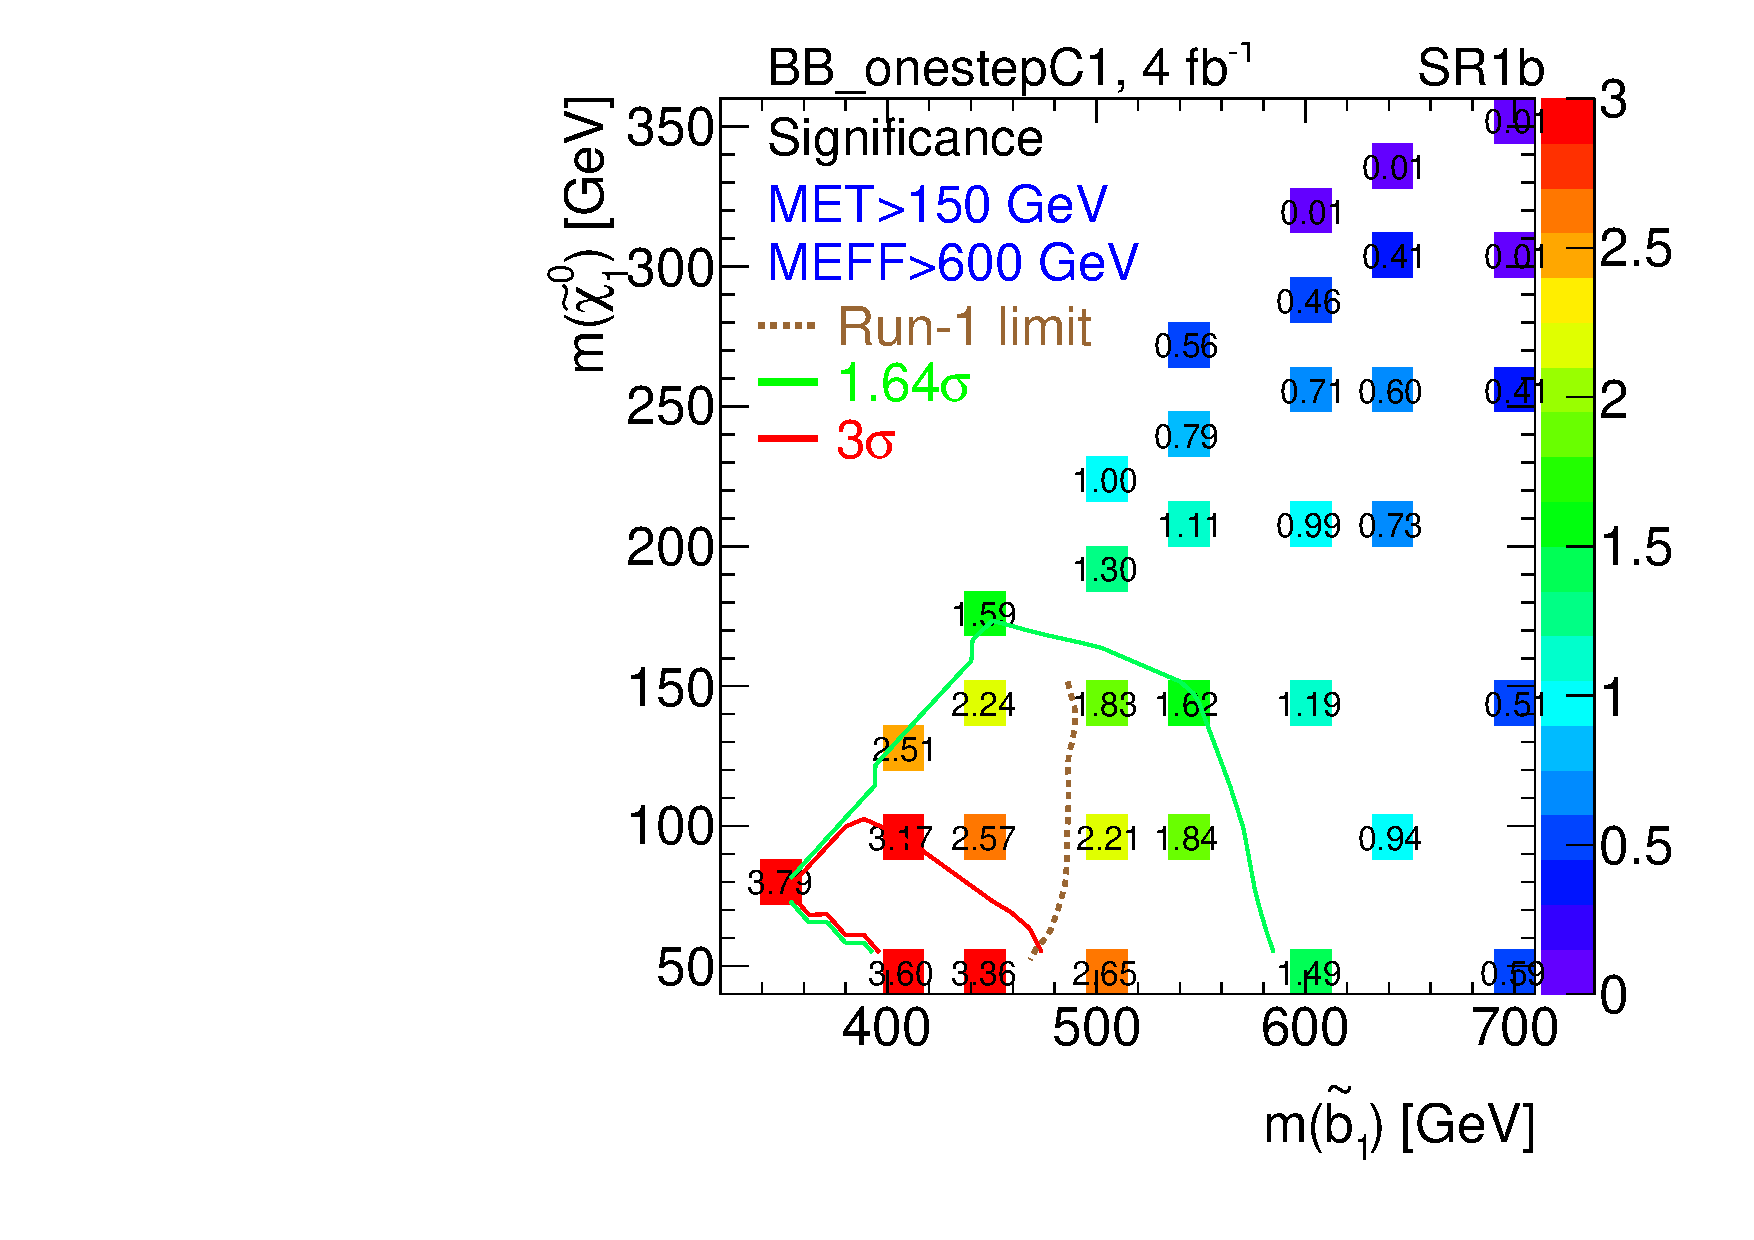
\includegraphics[width=0.4\textwidth]{OPTIMIZATION/Optimiz_SR1b_4fb_150_600.pdf}
  \includegraphics[width=0.4\textwidth]{OPTIMIZATION/Optimiz_SR3b_4fb_125_700.pdf}\\
  \includegraphics[width=0.4\textwidth]{OPTIMIZATION/Optimiz_SR0b5j_4fb_125_700.pdf}
  \includegraphics[width=0.4\textwidth]{OPTIMIZATION/Optimiz_SR0b3j_4fb_200_600.pdf}
  \caption{Discovery significance for the SRs defined in Table~\ref{tab:SRdef4} (4~\ifb) for SR1b in the $\sbot\sbot^*\to t\bar t\tilde\chi_1^+\tilde\chi_1^-$ grid (top left), SR3b in the $\gluino\gluino\to t\bar tt\bar t\ninoone\ninoone$ grid (top right), SR0b5j in the $\gluino\gluino$ with $\gluino\to q\bar{q}'WZ\ninoone$ grid (bottom left) and SR0b3j in the $\gluino\gluino$ with $\gluino\to q\bar{q}(\ell\ell/\ell\nu)\ninoone$ grid (bottom right). The Run-1 limits in those models are shown with a brown line, and the 1.64$\sigma$ and 3$\sigma$ discovery contours from the proposed signal regions are shown in green and red, respectively.}
\label{fig:OptimSig4}
\end{figure}


%\FloatBarrier



\section{Background estimation}
\label{sec:bkg}
Two main sources of SM background can be distinguished in this analysis. 
The first category is the reducible or detector background which includes 
events containing electrons with mis-measured charge, mainly from the production of top quark pairs, and events 
containing at least one non-prompt or fake lepton (FNP), which mainly originate from hadron decays in events containing 
top quarks, $W$ or $Z$ bosons. Data-driven methods used for the estimation
of this background are described in Section~\ref{sec:DD_bkg}. The second category consists of events 
with two same-sign prompt leptons or at least three prompt leptons and is 
estimated using the MC samples described in Section~\ref{sec:dataMC}. 
Since diboson and $\ttbar V$ events are the main backgrounds in the signal regions, 
dedicated validation regions (VR) with an enhanced contribution from these processes 
are defined to verify the background predictions from the simulation (see Section~\ref{sec:valid}).


\subsection{Detector background estimation methods} 
\label{sec:DD_bkg}

Background events due to charge mis-identification concerns only the electron. The probability of mis-identifying the 
charge of a muon is checked in both data and MC simulation, and found to be negligible in the kinematic range relevant to this analysis.
The contribution of charge-flip events to the SR/VR yields is estimated using the data. 
The electron charge-flip probability is extracted in a $Z/\gamma^{*}\to ee$ data sample using a likelihood fit 
which takes as input the numbers of same-sign and opposite-sign electron pairs observed in a window around the $Z$ mass. 
The charge-flip probability is a free parameter of the fit and is extracted as a function of the electron $\pt$ and $\eta$. 
These probabilities are in the range \textcolor{red}{UPDATE:1--5\%} and \textcolor{red}{UPDATE:0.1--1\%} for the candidate 
and signal electrons respectively.
The event yield of this background in the signal or validation regions is obtained by applying the measured charge-flip probability 
to the data regions with the same kinematic requirements as the signal or validation regions but with opposite-sign lepton pairs. 

The contribution from fake or non-prompt leptons (such as hadrons mis-identified as leptons, 
leptons originating from heavy-flavour decays, and electrons from photon conversions) 
is also estimated from the data with a matrix method similar to that described in Ref.~\cite{SUSY3bjetsRun1}. 
In this method, two types of lepton identification criteria are defined: ``tight'', 
corresponding to the signal lepton criteria described in Section~\ref{sec:selection}, 
and ``loose'', corresponding to candidate leptons after overlap removal. 
The matrix method relates the number of events containing prompt or FNP leptons 
to the number of observed events with tight or loose-not-tight leptons 
using the probability for loose prompt or FNP leptons to satisfy the tight criteria. 
The probability for loose prompt leptons to satisfy the tight selection criteria ($\epsilon$)
is obtained using a $Z/\gamma^*\to\ell\ell$ data sample 
and is modelled as a function of the lepton $\pt$ and $\eta$. 
The probability for loose FNP leptons to satisfy the tight selection criteria (FNP fake rate, $f$) is determined from data 
in SS and three lepton control regions enriched in non-prompt leptons originating from heavy-flavour decays, mostly coming from 
semileptonic $\ttbar$ events. This region contains events with at least one $b$-jet, 
one well-isolated ``tag'' muon, and an additional loose electron or muon on which the measurement is performed. 
The efficiencies are measured as function of \pt ($\eta$ binning is also used for low \pt muons) 
after subtracting the small contribution from prompt lepton processes. 

\textcolor{red}{[UPDATE: rewrite/inflate this paragraph]}The estimated FNP yields in the SRs are consistent with those 
predicted by two alternative methods: the first one relies on MC simulation of processes with FNP leptons or charge-flipped electrons 
($\ttbar$, $V$+jets)~\cite{paperSS3L,ATLAS-CONF-2012-151}, 
corrected to match the observed data in dedicated control regions. 
The second method relies on data events with only one lepton, which are the processes leading to FNP leptons, 
to extrapolate from low-\met\ control regions to the SRs.

%The data-driven background estimates are cross-checked with an MC-based technique. 
%In this method, the contributions from processes with FNP leptons and electron charge mis-identification 
%are obtained from MC simulation and normalised to data in dedicated control regions at low jet multiplicity, low $\met$, and 
%either with or without $b$-jets. 
%The normalisation is performed using five multipliers: one to correct 
%the electron charge mis-identification rate, and four to correct the contributions from FNP 
%electrons or muons originating from $b$-jets or light-flavour jets, respectively.
%In addition to the MC samples listed in Section~\ref{sec:dataMC}, this method employs samples of top quark pair production generated with the \POWHEG-Box v2 generator interfaced to \PYTHIA 6.428~\cite{Sjostrand:2006za}, 
%as well as samples of simulated $W$+jets and $Z$+jets events generated with \POWHEG-Box v2 interfaced to \PYTHIA 8.186.

% not the best place, but otherwise it's not well positionned wrt the text...
\begin{figure}[th!]
\centering
\begin{subfigure}[t]{0.49\textwidth}\includegraphics[width=\textwidth]{DILEP_2JMET50_njets25}\caption{}\end{subfigure}
\begin{subfigure}[t]{0.49\textwidth}\includegraphics[width=\textwidth]{DILEP_2JMET50_nbjets}\caption{}\end{subfigure}
\begin{subfigure}[t]{0.49\textwidth}\includegraphics[width=\textwidth]{EE_2JMET50_meff}\caption{}\end{subfigure}
\begin{subfigure}[t]{0.49\textwidth}\includegraphics[width=\textwidth]{TRILEP_2JMET50_meff}\caption{}\end{subfigure}
\caption{
Distributions of the number of jets, of $b$-tagged jets and the effective mass after requiring at least two jets ($\pT>\SI{25}{GeV}$) and $\met>\SI{50}{GeV}$, 
as well as at least two same-sign leptons (a,b) or two same-sign electrons (c) or three leptons (d). 
The statistical uncertainties in the background prediction are included in the uncertainty band, 
as well as the full systematic uncertainties for backgrounds with fake or non-prompt leptons, or charge-flip. 
The light blue bands in the ratio plots show contributions from statistical uncertainties alone while the hashed area shows the total uncertainty.. 
The ``Rare'' category contains the contributions from associated production $\ttbar+WW/WZ$, 
as well as $t+Z/WZ/\ttbar$, $H+W/Z$, and triboson production. \textcolor{red}{[UPDATE: Remove numbers in the legend 
and move from upper case to lower case.]}
}
\label{fig:Bkg_distribs} 
\end{figure} 


\subsection{Validation of background estimates}
\label{sec:valid}

To check the validity and robustness of the background estimates, 
the distributions of several discriminating variables in data are compared 
with the predicted background after various requirements on the number of jets and $b$-jets. 
%Events are categorised based on the flavours of the selected leptons, and the different flavour channels are compared separately. 
Examples of such distributions are shown in Fig.~\ref{fig:Bkg_distribs}, 
and illustrate that the predictions and data agree fairly well. 

Dedicated validation regions are defined to test the estimate of the $\ttbar V$, $WZ$ and $W^\pm W^\pm$ SM processes contributing to the signal regions. The corresponding selections are summarized in Table~\ref{tab:VRdef}. 
In these regions, the overlap with the signal regions is resolved by vetoing events that contribute to the signal regions.  
%To further reduce contributions from electron charge mis-identification,  events are also vetoed in VR-$\ttbar W$ and VR-$W^\pm W^{\pm}jj$ if one of the two leading leptons is an electron with $|\eta|>1.37$\textcolor{red}{[UPDATE:Still true]}, since contributions from charge-flip electrons are smaller in the central region due to the lower amount of detector material in front of the calorimeters. 
The purity of the targeted processes in these regions ranges from about \textcolor{red}{[UPDATE:20\% to $50\%$]}. 

The observed yields in these validation regions, compared with the background predictions and uncertainties, 
can be seen in Table~\ref{tab:VR_yields}.
%, and the effective mass distributions are shown in Fig.~\ref{fig:VRd}--\ref{fig:VRf}.
There is good agreement between data and the estimated background for the validation regions.

\begin{table}[t!]
\hspace{0.5cm}
\def\arraystretch{1.1}
\centering
\resizebox{\textwidth}{!}
{\small
\begin{tabular}{|c|c|c|c|c|c|c|l|}
\hline    
Validation        &  $N_{\rm{lepton}}^{\rm{signal}}$ ($N_{\rm{lepton}}^{\rm{cand}}$)   & $N_{b\rm{-jets}}$  &  $N_{\rm{jets}}$  & $p^{}_{\rm{T,jet}}$  & \met\ & \meff\  & Other \\
Region Name       &  &  &  & [GeV]  & [GeV] & [GeV]  & \\
\hline\hline
$W^{\pm} W^{\pm}jj$ & $=2$ ($=2$)    &  $=0$ & $\geq 2$ &   $>50$ & $> 55$  & $> 650$ & veto $81<\mee<101$~GeV  \\
               	  & $=1$ SS pair  &	  &	     &         &   	&	  & $\pt^{\ell_2}>30$~GeV \\
               	  &		  &	  &	     &         &   	&	  & min$\left\{\Delta R(\ell_{1,2},j)\right\}>0.7$ \\
               	  &		  &	  &	     &         &   	&	  & min$\left\{\Delta R(\ell_1, \ell_2)\right\}>1.3$ \\
\hline
$WZ$4j            & $=3$ ($=3$)    &  $=0$ & $\geq 4$ &  $>25$   & --    & $> 450$ & $\met/\sum p_T^{\ell} < 0.7$ \\
\hline
$WZ$5j            & $=3$ ($=3$)    &  $=0$ & $\geq 5$ &  $>25$   & --    & $> 450$ & $\met/\sum p_T^{\ell} < 0.7$  \\ 
\hline
$\ttbar W$   	&$=2$ ($=2$)    &$\geq 1$   & $\geq 4$ ($e^\pm e^\pm$, $e^\pm \mu^\pm$) & $>40$ & $> 45$  & $> 550$   & $\pt(\ell_2)>40$~GeV\\
              	& $=1$ SS pair  &       &  $\geq 3$ ($\mu^\pm \mu^\pm$)   &  $>25$ &      &          & $\sum p_T^{b-jet}/\sum p_T^{jet}>0.25$ \\ 
\hline
$\ttbar Z$    	&$\geq 3$ (-) & $\geq 1$ & $\geq 3$ &  $>35$ &  --    & $> 450$  & $81<m_\text{SFOS}<101$~GeV \\
                &$\geq 1$ SFOS pair&     &          &       &         &         &  \\
\hline
All VRs & \multicolumn{7}{c|}{Veto events belonging to any SR} \\
\hline
\end{tabular}
}
\caption{Summary of the event selection in the validation regions (VRs). 
Requirements are placed on the number of signal leptons ($N_{\rm{lept}}^{\rm{signal}}$) 
and candidate leptons ($N_{\rm{lept}}^{\rm{cand}}$), the number of jets ($N_{\rm{jets}}$) 
or the number of $b$-jets with $\pt>\SI{20}{GeV}$ ($N_{b\rm{-jets}}$). The two leading-\pt 
leptons are referred to as $\ell_{1,2}$ with decreasing \pt. Additional requirements are set 
on \met, \meff, the invariant mass of the two leading electrons $m_{ee}$, the presence of SS 
leptons or a pair of same-flavour opposite-sign leptons (SFOS) and its invariant mass $m_\text{SFOS}$. 
A minimum angular separation between the leptons and the jets ($\Delta R (\ell, j)$) and between the two 
leptons ($\Delta R (\ell_{1}, \ell_2)$) is imposed in $W^\pm W^\pm$ VR. For the two $WZ$ VRs an upper cut 
on the ratio between the \met in the event and the sum of all selected leptons \pt (\met/$\sum{p_T^\ell}$) is required. 
An upper cut on the ratio between the sum of the \pt of all $b$-jets and that of all jets in the event ($\sum p_T^{b-j} / \sum{p_T^{j}}$) is 
considered only in the $\ttbar W$ VR.
}
\label{tab:VRdef}
\end{table}

\begin{table}[t!]
\hspace{0.5cm}
\def\arraystretch{1.1}
\centering
%\resizebox{\textwidth}{!}
%{\small
\begin{tabular}{|l|c|c|c|c|c|}
\hline    
 Validation Regions       & $WZ$4j & $WZ$5j  & $W^\pm W^{\pm}jj$& $\ttbar W$   & $\ttbar Z$  \\
\hline\hline
$t\bar{t}Z/\gamma^*$     & $  \pm  $ & $  \pm  $      & $  \pm  $  & $  \pm  $    & $  \pm  $  \\
$t\bar{t}W$              & $  \pm $  & $  \pm  $      & $  \pm  $  & $  \pm  $    & $  \pm  $  \\
$t\bar{t}H$              & $  \pm $  & $  \pm  $      & $  \pm  $  & $  \pm  $    & $  \pm  $  \\
$t\bar{t}t\bar{t}$       & $  \pm $  & $  \pm  $      & $  \pm  $  & $  \pm  $    & $  \pm  $  \\
$WW$                     & $  \pm $  & $  \pm  $      & $  \pm  $  & $  \pm  $    & $  \pm  $  \\
$WZ$                     & $  \pm $  & $  \pm  $      & $  \pm  $  & $  \pm  $    & $  \pm  $  \\
$ZZ$                     & $  \pm $  & $  \pm  $      & $  \pm  $  & $  \pm  $    & $  \pm  $  \\
Rare                     & $  \pm  $ & $  \pm  $      & $  \pm  $  & $  \pm  $    & $  \pm  $  \\
Fake/non-prompt leptons  & $  \pm  $ & $  \pm  $      & $  \pm  $  & $  \pm  $    & $  \pm $  \\
Charge-flip              & $-$       & $  \pm  $      & $  \pm  $  & $  \pm  $    & $-$  \\
\hline
Total SM  background   	& $-$        & $  \pm  $      & $  \pm  $  & $  \pm  $    & $-$  \\
\hline
Observed	   	& $-$        & $  \pm  $      & $  \pm  $  & $  \pm  $    & $-$  \\
\hline
\end{tabular}
%}
\caption{The numbers of observed data and expected background events in the validation regions. 
The ``Rare'' category contains the contributions from associated production $\ttbar+WW/WZ$, 
as well as $t+Z/WZ/\ttbar$, $H+W/Z$, and triboson production. Background categories shown as a ``$-$'' 
denote that they cannot contribute to a given region (e.g. charge flips in 3-lepton regions). 
The displayed yields include all sources of statistical and systematic uncertainties, 
except for the theoretical uncertainties which only affect the inclusive production cross-sections.}
\label{tab:VR_yields}
\end{table}

\section{Systematic uncertainties on the background estimation}
\label{sec:syst}

Figure~\ref{fig:PlotSR} summarises the contributions of the different sources of systematic uncertainty 
on the total SM background predictions in the signal regions.

The systematic uncertainties related to the same-sign prompt leptons background estimation 
arise from the accuracy of the theoretical and experimental modelling in the MC simulation.
The primary sources of systematic uncertainties are related to the jet energy scale calibration, 
jet energy resolution, $b$-tagging efficiency, and MC modelling and theoretical cross-section uncertainties. 
The statistical uncertainty of the simulated event samples is also taken into account.

The cross-sections used to normalise the MC samples are varied according to the uncertainty in the 
cross-section calculation, that is, 13\% for $\ttbar W$, 12\% for $\ttbar Z$ production~\cite{YR4}, 6\% for diboson
production~\cite{pubnote_mc_multiboson}, 8\% for $\ttbar H$~\cite{YR4} and 30\% for $\ttbar\ttbar$~\cite{Alwall:2014hca}. 
Additional uncertainties are assigned to some of these backgrounds to account for the theoritical modelling of the kinematic 
distributions in the MC simulation. For $\ttbar W$ and $\ttbar Z$, the predictions from the \AMCATNLO and \SHERPA generators are compared, 
and the renormalisation and factorisation scales used to generate these samples are varied, 
leading to a $\sim$\textcolor{red}{[UPDATE:30\%]} uncertainty on the expected SR yields for these processes. 
For dibosons, uncertainties are estimated by varying the renormalisation, factorisation and resummation scales, 
leading to a $\sim$\textcolor{red}{[UPDATE:40-50\%]} uncertainty for these processes after the SR selections. 
For $\ttbar H$, $\ttbar \ttbar$ and Rare production processes, a conservative 50\% uncertainty 
on their total contribution is assigned. 

Uncertainties in the FNP lepton background estimate are assigned due to the limited number 
of data events in the loose and tight lepton control regions.
In addition, systematic uncertainties of \textcolor{red}{[UPDATE:50-60\%]} are assigned to the FNP fake rate to account 
for potentially different 
compositions (heavy flavour, light flavour or conversions) between the regions used to measure these probabilities and the SRs, 
as well as the contamination from prompt leptons in the former regions. Similarly a \textcolor{red}{[UPDATE:5\%]} systematic is assigned to 
$\epsilon$ determination. This leads to overall FNP background uncertainties in the total background estimates 
of \textcolor{red}{[UPDATE:5--32\%]} depending on the signal region.

The uncertainty on the electron charge-flip probability mainly originates from the limited number of events used in 
the charge-flip probability measurement regions and the uncertainty related to the background subtraction 
beyond the $Z$ peak. The relative error on the charge-flip is below \textcolor{red}{[UPDATE:20\%]} for lepton \pt above 20 GeV.

\begin{figure}[H]
\begin{center}
\begin{subfigure}[t]{0.95\textwidth}\includegraphics[width=\textwidth]{SystematicsSummary}\caption{}\end{subfigure} \\
\begin{subfigure}[t]{0.87\textwidth}\includegraphics[width=\textwidth]{SRsummary}\caption{}\end{subfigure}
\end{center}
\caption{Relative systematic uncertainties and comparison of the observed and expected event yields in each signal region. 
The background expectations are those obtained from the background-only fits, presented in Table~\ref{tab:SR_yields}. 
\textcolor{red}{[UPDATE: Put all signal regions with final notations. Add ratio plot below SR Event Yields]}} 
\label{fig:PlotSR}
\end{figure}

%\begin{table}[h!]
%\begin{center}
%\caption{The main sources of systematic uncertainty on the SM background estimates for the four signal regions are shown 
%and their values given as relative uncertainties in the expected signal region background event yields. 
%The individual components can be correlated and therefore do not necessarily add up in quadrature to the total systematic uncertainty.
%For reference, the total number of expected background events is also shown.
%}
%\label{tab:SR_syst}
%{\small
%\begin{tabular}{lrrrr}
%\noalign{\smallskip}\hline\hline\noalign{\smallskip}
%         & SR0b3j         & SR0b5j     & SR1b & SR3b     \\[-0.05cm]
%\noalign{\smallskip}\hline\hline\noalign{\smallskip}
%Diboson theoretical uncertainties    & 23\%  &  16\%   &  1\%  &$<$1\%   \\
%$\ttbar V$ theoretical uncertainties & 3\%   &  4\%    & 13\%  &  9\%   \\
%Other theoretical uncertainties      & 5\%   &  3\%    &  9\%  & 15\%   \\
%\noalign{\smallskip}\hline\noalign{\smallskip}
%MC statistical uncertainties         & 11\%  &  14\%   &  3\%  &  6\%   \\
%\noalign{\smallskip}\hline\noalign{\smallskip}
%Jet energy scale        & 12\%   &  11\%  & 6\%    & 5\%   \\
%Jet energy resolution   & 3\%    &  9\%   & 2\%    & 3\%   \\
%$b$-tagging             & 4\%    &  6\%   & 3\%    & 10\%   \\
%PDF                     & 6\%    &  6\%   & 6\%    & 8\%   \\
%Fake/non-prompt leptons & 18\%    &  20\%   & 18\%   & 21\%   \\
%Charge flip             & --     & 1\% & 3\%    & 8\%   \\
%\noalign{\smallskip}\hline\noalign{\smallskip}
%Total background uncertainties & 30\%   & 34\%   & 22\%   & 31\%   \\
%\noalign{\smallskip}\hline\hline\noalign{\smallskip}
%Total background events & $1.5$ & $0.88$ & $4.5$ & $0.80$\\
%\noalign{\smallskip}\hline\hline\noalign{\smallskip}
%\end{tabular}
%}
%\end{center}
%\end{table}
	


\section{Validation of the background estimates}
\label{sec:bkg_validation}
The data-driven background estimates described previously are based on control regions that are kinematically different than the signal regions, as they contain less stringent requirements on the jet multiplicity, \met or \meff. 
It is therefore very important to validate them in busier and more energetic events. 
To do so we compare the background estimates to the data in regions where several kinematic variables are probed, after applying a certain selection~:
\begin{itemize}
	\item{Loose: requiring at least two same-sign signal leptons in the event.}
	\item{Intermediate: adding soft cuts i.e. at least one or two signal jets or $b$ jets.}
	\item{Hard: increase the number of jets in the event.} 
\end{itemize}  
These distributions are shown in section~\ref{sec:bkg_VP_DD_estimates}.  

%In section~\ref{sec:bkg_VP_3b_MC} we show another validation of background estimates in regions with 3 $b$-jets and opposite-sign leptons.

Beside these ``data-to-MC'' plots, several validation regions are also designed, and their definition is a balance between high purity, large statistics and low signal contamination. Their definition and the obtained results are presented in section~\ref{sec:bkg_VR}. 

Finally, section~\ref{subs:Results_AuxSR} presents the results in the auxiliary signal regions.
   
%%%%%%%%%%%%%%%%%%%%%%%
\subsection{Validation of the data-driven estimates} 
\label{sec:bkg_VP_DD_estimates}

Several distributions are shown for $L=3.2$ fb$^{-1}$ in combined or separate lepton channels, for a complete validation of the background estimates.The statistical uncertainties on the background prediction are included in the uncertainty band, as well as the theory uncertainties for the backgrounds with prompt SS/3L, and the full systematic uncertainties for data-driven backgrounds. The lepton selection implies that the signal definitions presented in Table~\ref{tab:lepdef} are satisfied. At least two light jets with \pt~$>$~25~\GeV and \met~$>$~60~\GeV are required to reduce the contributions from $Z$ and $W$ plus jets processes which are not present in the signal regions. 

\par {\bf Distributions in the $ee+e\mu+\mu\mu$ channel \\}
Figure~\ref{Fig:VP_allCh_bIncl_Njets_and_other} show several kinematic distributions 
after lepton selection, without any requirement on the number of $b$-jets. It shows the number of ($b$-) jets with \pt~$>$~50~GeV (20~GeV), the transverse mass computed with the leading lepton, 
the $H_T$ computed with all signal leptons and signal jets with \pt~$>$~20~\GeV in the event and the leading (subleading) lepton \pt.

\par {\bf Distributions in the $ee$ channel \\} 
Several distributions are shown in the $ee$ channel after the lepton selection with at least one $b$-jet (Figures~\ref{Fig:VP_ee_1b_Met}-\ref{Fig:VP_ee_1b_Njets_and_other}) 
and with a $b$-jet veto (Figures~\ref{Fig:VP_ee_0b_Met}-\ref{Fig:VP_ee_0b_Njets_and_other}). 
Additional cuts on the number of jets are added for some distributions to vary the fake lepton composition, and be closer to the signal regions. 

For the selections enriched in $b$-jets, the effective mass distribution is shown in Figure~\ref{Fig:VP_ee_1b_Meff} 
and the missing transverse energy distribution in Figure~\ref{Fig:VP_ee_1b_Met}. 
The distributions of the number of ($b$-) jets with \pt~$>$~25~GeV, the transverse mass computed with the leading lepton, the selected leptons \pt and the leading (subleading) lepton \pt are illustrated in Figure~\ref{Fig:VP_ee_1b_Njets_and_other}. 
Same distributions (following the same order) are shown also for the case with a $b$-jet veto.

\par {\bf Distributions in the $e\mu$ channel \\}
The kinematic distributions in the $e\mu$ channel are shown in Figures~\ref{Fig:VP_em_1b_Met}-\ref{Fig:VP_em_0b_Njets_and_other} after the lepton selection with at least one $b$-jet and with a $b$-jet veto. As in the previous case, additional cuts on the number of jets are added for the \meff\ and \met\ distributions. Same plots as in the $ee$ channel (retaining the same order) are shown. 

\par {\bf Distributions in the $\mu\mu$ channel \\}
Figures~\ref{Fig:VP_mm_1b_Met}-\ref{Fig:VP_mm_0b_Njets_and_other} present the distributions of the key kinematic variables in the $\mu\mu$ channel, 
similarly to the other channels. 

\par{\bf Discussion\\}
One can observe (mostly from the $ee$ channel) that the charge flip estimate agrees well with observed data. 
The fake lepton estimate agrees reasonably well with data in event selections requiring at least one $b$-jet; 
however the selections with a $b$-jet veto show a poor agreement (mostly the $e\mu$ channel), as the estimated yields of fake leptons clearly overshoot observed data. 

For a better validation of the background estimation in events with three leptons, the agreement between the observed number of data events and SM background is checked in regions with at least three leptons, at least two light jets with \pt~$>$~25~\GeV and \met~$>$~60~\GeV. Figures~\ref{Fig:VP_Nlep_3Lep}-\ref{Fig:VP_PtLep_3Lep} show the distribution of number of leptons, and the \pt of the third lepton in a region with at least one $b$-jet and at least 0 $b$-jets. Overall, the agreement is good. 


%%%%% all channels combined, no b-jet cut
%% 
\begin{figure}[h!]
\centering
\subfigure{
\includegraphics[width=0.45\textwidth]{BKG/validationPLots/NJETS50_LEP}
\includegraphics[width=0.45\textwidth]{BKG/validationPLots/NBJETS20_LEP}
}
\subfigure{
\includegraphics[width=0.45\textwidth]{BKG/validationPLots/MT_LEP_NOBJETCUT}
\includegraphics[width=0.45\textwidth]{BKG/validationPLots/HT_LEP_NOBJETCUT}
}
\subfigure{
\includegraphics[width=0.45\textwidth]{BKG/validationPLots/PTLEP_LEAD_NOBJETCUT}
\includegraphics[width=0.45\textwidth]{BKG/validationPLots/PTLEP_SUBLEAD_NOBJETCUT}
}
\caption{$ee+e\mu+\mumu$ channel, \met $>$ 60\GeV and $N_{jets}^{25}$~$\ge$2: Distributions of  jet multiplicity (\pt~$>$~50~GeV) (top-left), $b$-jet multiplicity (\pt~$>$~20~GeV) (top-right), \mt (middle-left), $H_T$ (middle-right), leading lepton \pt (bottom-left) and subleading lepton \pt (bottom-right) after lepton selections.}
\label{Fig:VP_allCh_bIncl_Njets_and_other}
\end{figure} 

\FloatBarrier


%%%%% ee channel, >= 1 b-jet
\begin{figure}[h!]
\centering
\subfigure{
\includegraphics[width=0.5\textwidth]{BKG/validationPLots/MEFF_EE_LEP}
\includegraphics[width=0.5\textwidth]{BKG/validationPLots/MEFF_EE_L1JET}
}
\subfigure{
\includegraphics[width=0.5\textwidth]{BKG/validationPLots/MEFF_EE_L2JET}
\includegraphics[width=0.5\textwidth]{BKG/validationPLots/MEFF_EE_L3JET}
}
\caption{$ee$ channel, \met $>$ 60\GeV and $N_{jets}^{25}$~$\ge$2: Effective mass distribution after lepton selections with at least one $b$-jet (\pt~$>$~20~GeV) and with at least 0, 1, 2 and 3 jets with \pt~$>$~40~GeV (from top-left to bottom-right).}
\label{Fig:VP_ee_1b_Meff}
\end{figure}
%%
\begin{figure}[h!]
\centering
\subfigure{
\includegraphics[width=0.5\textwidth]{BKG/validationPLots/MET_EE_LEP}
\includegraphics[width=0.5\textwidth]{BKG/validationPLots/MET_EE_L1JET}
}
\subfigure{
\includegraphics[width=0.5\textwidth]{BKG/validationPLots/MET_EE_L2JET}
\includegraphics[width=0.5\textwidth]{BKG/validationPLots/MET_EE_L3JET}
}
\caption{$ee$ channel, \met $>$ 60\GeV and $N_{jets}^{25}$~$\ge$2: Missing transverse energy distribution after lepton selections with at least one $b$-jet (\pt~$>$~20~GeV) and with at least 0, 1, 2 and 3 jets with \pt~$>$~40~GeV (from top-left to bottom-right).}
\label{Fig:VP_ee_1b_Met}
\end{figure}
%%
\begin{figure}[h!]
\centering
\subfigure{
\includegraphics[width=0.45\textwidth]{BKG/validationPLots/NJETS40_EE_LEP}
\includegraphics[width=0.45\textwidth]{BKG/validationPLots/NBJETS20_EE_LEP}
}
\subfigure{
\includegraphics[width=0.45\textwidth]{BKG/validationPLots/MT_EE_LEP}
\includegraphics[width=0.45\textwidth]{BKG/validationPLots/PTLEP_EE_LEP}
}
\subfigure{
\includegraphics[width=0.45\textwidth]{BKG/validationPLots/PTLEP_EE_LEAD}
\includegraphics[width=0.45\textwidth]{BKG/validationPLots/PTLEP_EE_SUBLEAD}
}
\caption{$ee$ channel, \met $>$ 60\GeV and $N_{jets}^{25}$~$\ge$2: Distributions of  jet multiplicity (\pt~$>$~25~GeV) (top-left) and $b$-jet multiplicity (\pt~$>$~20~GeV) (top-right) after lepton selection, and of \mt (middle-left), selected leptons \pt (middle-right), leading lepton \pt (bottom-left) and subleading lepton \pt (bottom-right) after lepton selections with at least one $b$-jet (\pt~$>$~20~GeV).}
\label{Fig:VP_ee_1b_Njets_and_other}
\end{figure} 




%%%%% ee channel, ==0 b-jet
\begin{figure}[h!]
\centering
\subfigure{
\includegraphics[width=0.5\textwidth]{BKG/validationPLots/MEFF_EE_BVETOLEP}
\includegraphics[width=0.5\textwidth]{BKG/validationPLots/MEFF_EE_BVETOL1JET}
}
\subfigure{
\includegraphics[width=0.5\textwidth]{BKG/validationPLots/MEFF_EE_BVETOL2JET}
\includegraphics[width=0.5\textwidth]{BKG/validationPLots/MEFF_EE_BVETOL3JET}
}
\caption{$ee$ channel, \met $>$ 60\GeV and $N_{jets}^{25}$~$\ge$2: Effective mass distribution after lepton selections with a $b$-jet veto (\pt~$>$~20~GeV) and with at least 0, 1, 2 and 3 jets with \pt~$>$~40~GeV (from top-left to bottom-right).}
\label{Fig:VP_ee_0b_Meff}
\end{figure}
%%
\begin{figure}[h!]
\centering
\subfigure{
\includegraphics[width=0.5\textwidth]{BKG/validationPLots/MET_EE_BVETOLEP}
\includegraphics[width=0.5\textwidth]{BKG/validationPLots/MET_EE_BVETOL1JET}
}
\subfigure{
\includegraphics[width=0.5\textwidth]{BKG/validationPLots/MET_EE_BVETOL2JET}
\includegraphics[width=0.5\textwidth]{BKG/validationPLots/MET_EE_BVETOL3JET}
}
\caption{$ee$ channel, \met $>$ 60\GeV and $N_{jets}^{25}$~$\ge$2: Missing transverse energy distribution after lepton selections with a $b$-jet veto (\pt~$>$~20~GeV) and with at least 0, 1, 2 and 3 jets with \pt~$>$~40~GeV (from top-left to bottom-right).}
\label{Fig:VP_ee_0b_Met}
\end{figure}
%%
\begin{figure}[h!]
\centering
\subfigure{
\includegraphics[width=0.5\textwidth]{BKG/validationPLots/MT_EE_BVETOLEP}
\includegraphics[width=0.5\textwidth]{BKG/validationPLots/PTLEP_EE_BVETOLEP}
}
\subfigure{
\includegraphics[width=0.5\textwidth]{BKG/validationPLots/PTLEP_EE_BVETOLEAD}
\includegraphics[width=0.5\textwidth]{BKG/validationPLots/PTLEP_EE_BVETOSUBLEAD}
}
\caption{$ee$ channel, \met $>$ 60\GeV and $N_{jets}^{25}$~$\ge$2: Distributions of \mt (top-left), selected leptons \pt (top-right), leading lepton \pt (bottom-left) and subleading lepton \pt (bottom-right) after lepton selections with with a $b$-jet veto (\pt~$>$~20~GeV).}
\label{Fig:VP_ee_0b_Njets_and_other}
\end{figure} 

\FloatBarrier


%%%%% emu channel, >= 1 b-jet
\begin{figure}[h!]
\centering
\subfigure{
\includegraphics[width=0.5\textwidth]{BKG/validationPLots/MEFF_EM_LEP}
\includegraphics[width=0.5\textwidth]{BKG/validationPLots/MEFF_EM_L1JET}
}
\subfigure{
\includegraphics[width=0.5\textwidth]{BKG/validationPLots/MEFF_EM_L2JET}
\includegraphics[width=0.5\textwidth]{BKG/validationPLots/MEFF_EM_L3JET}
}
\caption{$e\mu$ channel, \met $>$ 60\GeV and $N_{jets}^{25}$~$\ge$2: Effective mass distribution after lepton selections with at least one $b$-jet (\pt~$>$~20~GeV) and with at least 0, 1, 2 and 3 jets with \pt~$>$~40~GeV (from top-left to bottom-right).}
\label{Fig:VP_em_1b_Meff}
\end{figure}
%%
\begin{figure}[h!]
\centering
\subfigure{
\includegraphics[width=0.5\textwidth]{BKG/validationPLots/MET_EM_LEP}
\includegraphics[width=0.5\textwidth]{BKG/validationPLots/MET_EM_L1JET}
}
\subfigure{
\includegraphics[width=0.5\textwidth]{BKG/validationPLots/MET_EM_L2JET}
\includegraphics[width=0.5\textwidth]{BKG/validationPLots/MET_EM_L3JET}
}
\caption{$e\mu$ channel, \met $>$ 60\GeV and $N_{jets}^{25}$~$\ge$2: Missing transverse energy distribution after lepton selections with at least one $b$-jet (\pt~$>$~20~GeV) and with at least 0, 1, 2 and 3 jets with \pt~$>$~40~GeV (from top-left to bottom-right).}
\label{Fig:VP_em_1b_Met}
\end{figure}
%%
\begin{figure}[h!]
\centering
\subfigure{
\includegraphics[width=0.45\textwidth]{BKG/validationPLots/NJETS40_EM_LEP}
\includegraphics[width=0.45\textwidth]{BKG/validationPLots/NBJETS20_EM_LEP}
}
\subfigure{
\includegraphics[width=0.45\textwidth]{BKG/validationPLots/MT_EM_LEP}
\includegraphics[width=0.45\textwidth]{BKG/validationPLots/PTLEP_EM_LEP}
}
\subfigure{
\includegraphics[width=0.45\textwidth]{BKG/validationPLots/PTLEP_EM_LEAD}
\includegraphics[width=0.45\textwidth]{BKG/validationPLots/PTLEP_EM_SUBLEAD}
}
\caption{$e\mu$ channel, \met $>$ 60\GeV and $N_{jets}^{25}$~$\ge$2: Distributions of  jet multiplicity (\pt~$>$~25~GeV) (top-left) and $b$-jet multiplicity (\pt~$>$~20~GeV) (top-right) after lepton selection, and of \mt (middle-left), selected leptons \pt (middle-right), leading lepton \pt (bottom-left) and subleading lepton \pt (bottom-right) after lepton selections with at least one $b$-jet (\pt~$>$~20~GeV).}
\label{Fig:VP_em_1b_Njets_and_other}
\end{figure} 




%%%%% emu channel, ==0 b-jet
\begin{figure}[h!]
\centering
\subfigure{
\includegraphics[width=0.5\textwidth]{BKG/validationPLots/MEFF_EM_BVETOLEP}
\includegraphics[width=0.5\textwidth]{BKG/validationPLots/MEFF_EM_BVETOL1JET}
}
\subfigure{
\includegraphics[width=0.5\textwidth]{BKG/validationPLots/MEFF_EM_BVETOL2JET}
\includegraphics[width=0.5\textwidth]{BKG/validationPLots/MEFF_EM_BVETOL3JET}
}
\caption{$e\mu$ channel, \met $>$ 60\GeV and $N_{jets}^{25}$~$\ge$2: Effective mass distribution after lepton selections with a $b$-jet veto (\pt~$>$~20~GeV) and with at least 0, 1, 2 and 3 jets with \pt~$>$~40~GeV (from top-left to bottom-right).}
\label{Fig:VP_em_0b_Meff}
\end{figure}
%%
\begin{figure}[h!]
\centering
\subfigure{
\includegraphics[width=0.5\textwidth]{BKG/validationPLots/MET_EM_BVETOLEP}
\includegraphics[width=0.5\textwidth]{BKG/validationPLots/MET_EM_BVETOL1JET}
}
\subfigure{
\includegraphics[width=0.5\textwidth]{BKG/validationPLots/MET_EM_BVETOL2JET}
\includegraphics[width=0.5\textwidth]{BKG/validationPLots/MET_EM_BVETOL3JET}
}
\caption{$e\mu$ channel, \met $>$ 60\GeV and $N_{jets}^{25}$~$\ge$2: Missing transverse energy distribution after lepton selections with a $b$-jet veto (\pt~$>$~20~GeV) and with at least 0, 1, 2 and 3 jets with \pt~$>$~40~GeV (from top-left to bottom-right).}
\label{Fig:VP_em_0b_Met}
\end{figure} 
%%
\begin{figure}[h!]
\centering
\subfigure{
\includegraphics[width=0.5\textwidth]{BKG/validationPLots/MT_EM_BVETOLEP}
\includegraphics[width=0.5\textwidth]{BKG/validationPLots/PTLEP_EM_BVETOLEP}
}
\subfigure{
\includegraphics[width=0.5\textwidth]{BKG/validationPLots/PTLEP_EM_BVETOLEAD}
\includegraphics[width=0.5\textwidth]{BKG/validationPLots/PTLEP_EM_BVETOSUBLEAD}
}
\caption{$e\mu$ channel, \met $>$ 60\GeV and $N_{jets}^{25}$~$\ge$2: Distributions of \mt (top-left), selected leptons \pt (top-right), leading lepton \pt (bottom-left) and subleading lepton \pt (bottom-right) after lepton selections with with a $b$-jet veto (\pt~$>$~20~GeV).}
\label{Fig:VP_em_0b_Njets_and_other}
\end{figure} 

\FloatBarrier


%%%%% mumu channel, >= 1 b-jet
\begin{figure}[h!]
\centering
\subfigure{
\includegraphics[width=0.5\textwidth]{BKG/validationPLots/MEFF_MM_LEP}
\includegraphics[width=0.5\textwidth]{BKG/validationPLots/MEFF_MM_L1JET}
}
\subfigure{
\includegraphics[width=0.5\textwidth]{BKG/validationPLots/MEFF_MM_L2JET}
\includegraphics[width=0.5\textwidth]{BKG/validationPLots/MEFF_MM_L3JET}
}
\caption{$\mu\mu$ channel, \met $>$ 60\GeV and $N_{jets}^{25}$~$\ge$2: Effective mass distribution after lepton selections with a $b$-jet veto (\pt~$>$~20~GeV) and with at least 0, 1, 2 and 3 jets with \pt~$>$~40~GeV (from top-left to bottom-right).}
\label{Fig:VP_mm_1b_Meff}
\end{figure}
%%
\begin{figure}[h!]
\centering
\subfigure{
\includegraphics[width=0.5\textwidth]{BKG/validationPLots/MET_MM_LEP}
\includegraphics[width=0.5\textwidth]{BKG/validationPLots/MET_MM_L1JET}
}
\subfigure{
\includegraphics[width=0.5\textwidth]{BKG/validationPLots/MET_MM_L2JET}
\includegraphics[width=0.5\textwidth]{BKG/validationPLots/MET_MM_L3JET}
}
\caption{$\mu\mu$ channel, \met $>$ 60\GeV and $N_{jets}^{25}$~$\ge$2: Missing transverse energy distribution after lepton selections with a $b$-jet veto (\pt~$>$~20~GeV) and with at least 0, 1, 2 and 3 jets with \pt~$>$~40~GeV (from top-left to bottom-right).}
\label{Fig:VP_mm_1b_Met}
\end{figure}
%%
\begin{figure}[h!]
\centering
\subfigure{
\includegraphics[width=0.45\textwidth]{BKG/validationPLots/NJETS40_MM_LEP}
\includegraphics[width=0.45\textwidth]{BKG/validationPLots/NBJETS20_MM_LEP}
}
\subfigure{
\includegraphics[width=0.45\textwidth]{BKG/validationPLots/MT_MM_LEP}
\includegraphics[width=0.45\textwidth]{BKG/validationPLots/PTLEP_MM_LEP}
}
\subfigure{
\includegraphics[width=0.45\textwidth]{BKG/validationPLots/PTLEP_MM_LEAD}
\includegraphics[width=0.45\textwidth]{BKG/validationPLots/PTLEP_MM_SUBLEAD}
}
\caption{$\mu\mu$ channel, \met $>$ 60\GeV and $N_{jets}^{25}$~$\ge$2: Distributions of  jet multiplicity (\pt~$>$~25~GeV) (top-left) and $b$-jet multiplicity (\pt~$>$~20~GeV) (top-right) after lepton selection, and of \mt (middle-left), selected leptons \pt (middle-right), leading lepton \pt (bottom-left) and subleading lepton \pt (bottom-right) after lepton selections with at least one $b$-jet (\pt~$>$~20~GeV).}
\label{Fig:VP_mm_1b_Njets_and_other}
\end{figure} 



%%%%% mumu channel, ==0 b-jet
\begin{figure}[h!]
\centering
\subfigure{
\includegraphics[width=0.5\textwidth]{BKG/validationPLots/MEFF_MM_BVETOLEP}
\includegraphics[width=0.5\textwidth]{BKG/validationPLots/MEFF_MM_BVETOL1JET}
}
\subfigure{
\includegraphics[width=0.5\textwidth]{BKG/validationPLots/MEFF_MM_BVETOL2JET}
\includegraphics[width=0.5\textwidth]{BKG/validationPLots/MEFF_MM_BVETOL3JET}
}
\caption{$\mu\mu$ channel, \met $>$ 60\GeV and $N_{jets}^{25}$~$\ge$2: Effective mass distribution after lepton selections with a $b$-jet veto (\pt~$>$~20~GeV) and with at least 0, 1, 2 and 3 jets with \pt~$>$~40~GeV (from top-left to bottom-right).}
\label{Fig:VP_mm_0b_Meff}
\end{figure}
%%
\begin{figure}[h!]
\centering
\subfigure{
\includegraphics[width=0.5\textwidth]{BKG/validationPLots/MET_MM_BVETOLEP}
\includegraphics[width=0.5\textwidth]{BKG/validationPLots/MET_MM_BVETOL1JET}
}
\subfigure{
\includegraphics[width=0.5\textwidth]{BKG/validationPLots/MET_MM_BVETOL2JET}
\includegraphics[width=0.5\textwidth]{BKG/validationPLots/MET_MM_BVETOL3JET}
}
\caption{$\mu\mu$ channel, \met $>$ 60\GeV and $N_{jets}^{25}$~$\ge$2: Missing transverse energy distribution after lepton selections with a $b$-jet veto (\pt~$>$~20~GeV) and with at least 0, 1, 2 and 3 jets with \pt~$>$~40~GeV (from top-left to bottom-right).}
\label{Fig:VP_mm_0b_Met}
\end{figure}
%%
\begin{figure}[h!]
\centering
\subfigure{
\includegraphics[width=0.5\textwidth]{BKG/validationPLots/MT_MM_BVETOLEP}
\includegraphics[width=0.5\textwidth]{BKG/validationPLots/PTLEP_MM_BVETOLEP}
}
\subfigure{
\includegraphics[width=0.5\textwidth]{BKG/validationPLots/PTLEP_MM_BVETOLEAD}
\includegraphics[width=0.5\textwidth]{BKG/validationPLots/PTLEP_MM_BVETOSUBLEAD}
}
\caption{$\mu\mu$ channel, \met $>$ 60\GeV and $N_{jets}^{25}$~$\ge$2: Distributions of \mt (top-left), selected leptons \pt (top-right), leading lepton \pt (bottom-left) and subleading lepton \pt (bottom-right) after lepton selections with with a $b$-jet veto (\pt~$>$~20~GeV).}
\label{Fig:VP_mm_0b_Njets_and_other}
\end{figure} 


%%%%%%%%%%%%%%%% 3 leptons %%%%%%%%%%%%%%%%%%%%%
\clearpage
\begin{figure}[h!]
\centering
\subfigure{
\includegraphics[width=0.5\textwidth]{BKG/validationPLots/NLEP20_EE_LEP}
\includegraphics[width=0.5\textwidth]{BKG/validationPLots/NLEP20_EM_LEP}
}
\subfigure{
\includegraphics[width=0.5\textwidth]{BKG/validationPLots/NLEP20_MM_LEP}}
\caption{\met $>$ 60\GeV and $N_{jets}^{25}$~$\ge$2 : Number of leptons distribution after lepton selection in $ee$ (left), $e\mu$ (middle) and $\mu\mu$ (right) channels.}
\label{Fig:VP_Nlep_3Lep}
\end{figure}
%%
\clearpage
\begin{figure}[h!]
\centering
\subfigure{
\includegraphics[width=0.5\textwidth]{BKG/validationPLots/PTLEP_EE_THIRDLEAD}
\includegraphics[width=0.5\textwidth]{BKG/validationPLots/PTLEP_EE_BVETOTHIRDLEAD}
}
\subfigure{
\includegraphics[width=0.5\textwidth]{BKG/validationPLots/PTLEP_EM_THIRDLEAD}
\includegraphics[width=0.5\textwidth]{BKG/validationPLots/PTLEP_EM_BVETOTHIRDLEAD}
}
\subfigure{
\includegraphics[width=0.5\textwidth]{BKG/validationPLots/PTLEP_MM_THIRDLEAD}
\includegraphics[width=0.5\textwidth]{BKG/validationPLots/PTLEP_MM_BVETOTHIRDLEAD}
}
\caption{3leptons, \met $>$ 60\GeV and $N_{jets}^{25}$~$\ge$2 : Third lepton \pt distribution after lepton selection with at least one $b$-jet (left) and 0 $b$-jets (right). Results are shown in $ee$ (left), $e\mu$ (middle) and $\mu\mu$ (right) channels.}
\label{Fig:VP_PtLep_3Lep}
\end{figure} 
  

\FloatBarrier

%%%%%%%%%%%%%%%%%%%%%%%%
%\subsection{Validation of background estimates with 3 $b$-jets}
%\label{sec:bkg_VP_3b_MC}
%
%We have a signal region, SR3b, which requires $\ge$3 $b$-jets of \pt~$>$~20~GeV, the background for which is determined both by data-driven estimates and Monte Carlo samples. In order to demonstrate that the $b$-tagging efficiencies in data are well modeled by Monte Carlo, including the mistag rate of light flavor jets, a higher statistics opposite-sign dilepton region with $\ge$3 $b$-jets is considered. Compared to the Monte Carlo samples used to obtain the validation plots from Section~\ref{sec:bkg_VP_DD_estimates}, extra samples have been considered to model the \ttbar, single top and $Z$+jets backgrounds.The (low) fake lepton background is estimated using Monte Carlo.
%
%Distributions were made with $b$-tagging calibration weights and shown in Figures~\ref{fig:3b_OS_MC_estim:meff_met}-\ref{fig:3b_OS_MC_estim:pt_jet}. 
%Generally the agreement between data and MC is rather good, although the statistics is very low. 
%
%% Distributions were made both with (Figure~\ref{}) and without (Figure~\ref{}) b-tagging calibration weights. The first important observation is that little changes between the two figures – thus we do not appear to be vulnerable to problems in the calibration that are known to exist for some samples. Further, it is seen that agreement is generally good. There are some kinematic discrepancies at large ** multiplicity, where the background over-predicts the data, however these can be safely ignored, as they are most likely due to issues in the ** Monte Carlo sample, which is not required for estimating the same-sign background. It is particularly encouraging that the b-jet pT distributions appear to agree well for low through to high \pt, and the b-jet multiplicity distribution indicates excellent agreement for exactly 3 b-jets.
%
%\begin{figure}[h!]
%\centering
%\subfigure{
%\includegraphics[width=0.5\textwidth]{fig_3b_OS_MC_Estim/MEFF_afterlepton_3b_0_physics}
%\includegraphics[width=0.5\textwidth]{fig_3b_OS_MC_Estim/MET_afterlepton_3b_0_physics}
%}
%\subfigure{
%\includegraphics[width=0.5\textwidth]{fig_3b_OS_MC_Estim/PTLEP1_afterlepton_3b_0_physics}
%\includegraphics[width=0.5\textwidth]{fig_3b_OS_MC_Estim/PTLEP2_afterlepton_3b_0_physics}
%}
%\caption{Distributions of effective mass (top-left), missing transverse momentum (top-right), leading lepton \pt (bottom-left) and subleading lepton \pt (bottom-right) after opposite-sign leptons selection with at least three $b$-jets. Only luminosity and MC statistical uncertainties are included.}
%\label{fig:3b_OS_MC_estim:meff_met}
%\end{figure} 
%%%
%\begin{figure}[h!]
%\centering
%\subfigure{
%\includegraphics[width=0.5\textwidth]{fig_3b_OS_MC_Estim/NLEP_afterlepton_3b_0_physics}
%\includegraphics[width=0.5\textwidth]{fig_3b_OS_MC_Estim/NBJET70_20_afterlepton_3b_0_physics}
%}
%\subfigure{
%\includegraphics[width=0.5\textwidth]{fig_3b_OS_MC_Estim/NJET30_afterlepton_3b_0_physics}
%\includegraphics[width=0.5\textwidth]{fig_3b_OS_MC_Estim/NJET40_afterlepton_3b_0_physics}
%}
%\caption{Distributions of number of leptons (top-left), number of $b$-jets with \pt~$>$~20~GeV (top-right), number of jets with \pt~$>$~30~GeV (bottom-left) and number of jets with \pt~$>$~40~GeV (bottom-right) after opposite-sign leptons selection with at least three $b$-jets. Only luminosity and MC statistical uncertainties are included.}
%\label{fig:3b_OS_MC_estim:nlep_njets}
%\end{figure} 
%%%
%\begin{figure}[h!]
%\centering
%\subfigure{
%\includegraphics[width=0.5\textwidth]{fig_3b_OS_MC_Estim/PTJET1_afterlepton_3b_0_physics}
%\includegraphics[width=0.5\textwidth]{fig_3b_OS_MC_Estim/PTBJET70_1_afterlepton_3b_0_physics}
%}
%\subfigure{
%\includegraphics[width=0.5\textwidth]{fig_3b_OS_MC_Estim/PTBJET70_2_afterlepton_3b_0_physics}
%\includegraphics[width=0.5\textwidth]{fig_3b_OS_MC_Estim/PTBJET70_3_afterlepton_3b_0_physics}
%}
%\caption{Distributions of number of leading jet \pt (top-right), leading $b$-jet \pt (top-left), subleading $b$-jet \pt (bottom-left) and third $b$-jet \pt (bottom-right) after opposite-sign leptons selection with at least three $b$-jets. Only luminosity and MC statistical uncertainties are included.}
%\label{fig:3b_OS_MC_estim:pt_jet}
%\end{figure} 
%

   
%%%%%%%%%%%%%%%%%%%%%%%
\subsection {Validation regions}
\label{sec:bkg_VR}
In this section the validation regions (VR) defined to check the prompt SS background are described. The observed number of data events and the corresponding background estimation are also shown at the end of the section. The definition of these validation regions is 
summarized in Table~\ref{tab:VRdef} and is detailed below. 
In all validation regions the signal regions defined in Table~\ref{tab:SRdef3} are vetoed to minimize the signal contamination and any overlap between the regions. As a \ttbar\ + $V$ validation region is very sensitive to models including third generation squarks (like direct sbottom pair production) we choose to veto any event passing SR2b defined in Table~\ref{tab:SRdefAux}. Given the excess observed in Run-1, we choose to veto also any event passing the SR3L3b (Table~\ref{tab:SRdefAux}) selection. The latter cut is applied in all validation regions. The ``signal removal'' cuts are shown with ``!SR'' in the tables.


\begin{table}[htb!]
\caption{Summary of the event selection in the validation regions. 
Requirements are placed on the number of signal leptons ($N_{\rm{lept}}^{\rm{signal}}$) and candidate leptons ($N_{\rm{lept}}^{\rm{cand}}$), 
%the number of jets with $\pt>\SI{25}{GeV}$ $\left(N_{\rm{jets}}^{25}\right)$ or the number of $b$-jets $\left(N_{b\rm{ jets}}^{20}\right)$. 
the number of jets with $\pt>\SI{25}{GeV}$ ($N_{\rm{jets}}^{25}$) or the number of $b$-jets with $\pt>\SI{20}{GeV}$ ($N_{b\rm{-jets}}^{20}$). 
The three leading \pt leptons are referred to as $\ell_{1,2,3}$ with decreasing \pt and the two leading jets as $j_{1,2}$.
Additional requirements are set on the invariant mass of the two leading electrons $m_{ee}$, 
the presence of SS leptons or a pair of same-flavour opposite-sign leptons (SFOS) and its invariant mass $m_\text{SFOS}$. 
}
\hspace{0.5cm}
\def\arraystretch{1.1}
\label{tab:VRdef}
\centering
\resizebox{\textwidth}{!}
{\small
\begin{tabular}{c|c|c|c|c|c|l}
\hline 
\hline    
          &  $N_{\rm{lept}}^{\rm{signal}}$ ($N_{\rm{lept}}^{\rm{cand}}$)   & $N_{b\rm{-jets}}^{20}$  &  $N_{\rm{jets}}^{25}$  & \met\ [GeV] & \meff\ [GeV]  & Other \\
\hline\hline
VR-WW   & =2 (=2) &  =0  &  $\geq$2 & 35--200  & 300--900 & $m(j_1 j_2)>500$~GeV\\
          & =1 SS pair    &      &             &         &         & $\pt(j_2)>40$~GeV\\
          &      &      &             &         &         & $\pt(\ell_2)>30$~GeV\\
%          &      &      &             &         &         & $|\eta(e_{1,2})|<1.37$\\
          &      &      &             &         &         & veto $80<m_{ee}<100$~GeV \\\hline
VR-WZ     & =3 (=3) &  =0  &  1--3     & 30--200  & $<$900 & $\pt(\ell_3)>30$~GeV \\ \hline
VR-ttV    &$\geq$2 (-) &$\geq$2&  $\geq$5 ($e^\pm e^\pm$,$e^\pm \mu^\pm$) & 20--200  & 200--900 & $\pt(\ell_2)>25$~GeV\\
          & $\geq$1 SS pair  &         &  $\geq$3 ($\mu^\pm \mu^\pm$)             &          &         & veto $\{\met>125$ and $\meff>\SI{650}{GeV}\}$\\ \hline %$|\eta(e_{1,2})|<1.37$\\ \hline
VR-ttZ    &$\geq$3 (-) & $\geq$1 & $\geq$4 ($=$1 $b$-jet)         & 20--150  & 100--900 & $\pt(\ell_2)>25$~GeV\\
          &$\geq$1 SFOS pair &         & $\geq$3 ($\geq$2 $b$-jets) &           &     & $\pt(\ell_3)>20$~GeV (if $e$)\\
%          &        &         &                           &          &         & $|\eta(e_{1,2})|<1.37$ \\
          &        &         &                           &          &         & $80<m_\text{SFOS}<100$~GeV \\
\hline\hline
All VRs & \multicolumn{6}{c}{Veto events belonging to any SR, or if $\ell_1$ or $\ell_2$ is an electron with $|\eta|>1.37$ (except in VR-WZ)}\\
\hline\hline
\end{tabular}
}
\end{table}


%%
\par{\bf \ttbar\ + $V$ background validation\\}
To validate the \ttbar\ + $Z$ and \ttbar\ + $W$ background estimation, several tentative regions defined with at least 1 or 2 $b$-jets in the event are optimized. Given the low statistics expected for 2-4\ifb no \ttbar\ + $W$ validation region could be proposed. A \ttbar\ + $Z$ enriched validation region ($ttZ$ 1bIncl) is defined in Table~\ref{tab:ttZ_VR} as a combination of two orthogonal regions, ``==1 $b$'' ($ttZ$ 1bExcl) and ``$\ge$2 $b$-jets'' ($ttZ$ 2bIncl). Beside the $b$-jet(s), at least three energetic signal leptons and at least 3 (4) soft jets (\pt~$>$~25~\GeV) are required in the event. A cut on the $Z$ boson mass ($80 < m^{SFOS}_{\ell\ell} < 100$~GeV) ensures a high purity, rejecting multi-boson processes. The fake lepton background is reduced with minimum cuts on \met\ and \meff, and with tight constraints on the electron acceptance ($|\eta|_{e1,2}$~$<$~1.37). The reached purity is 70\%. 

A second \ttbar\ + $V$ validation region ($ttV$ 2bIncl) is defined in Table~\ref{tab:ttV_VR} with at least two $b$-jets and at least two energetic signal leptons. The highest purity is found with at least five soft jets in the $ee$ and $e\mu$ channels, and at least three soft jets in the $\mu\mu$ channel. Cuts on \meff\  and electron acceptance ($|\eta|_{e1,2}$~$<$~1.37) are applied to reduce the detector background. The obtained purity is 50\%. 

In both validation regions the signal contamination is reduced by vetoing the signal regions (including SR2b and SR3L3b) and by 
applying upper cuts on \meff\ (900~GeV) and \met\ (150-200~GeV). 
Note that the \meff\ cut can be tighten to further decrease the SUSY contamination from models like direct sbottom. Using DC14 MC samples, in \ttbar\ + $Z$ VR it was found to be up to 27$\%$ when the direct-sbottom model was considered (sbottom mass of 550 \GeV) and up to 20$\%$ for direct squark (2 step) via sleptons with $W/Z$ bosons in the cascade decay, otherwise smaller than 10$\%$.   

\begin{table}[htb!]
\caption{\ttbar\ + $Z$ validation region definition ($ttZ$ 1bIncl = $ttZ$ 1bExcl || $ttZ$ 2bIncl).}
\label{tab:ttZ_VR}
\begin{center}
 \resizebox{\textwidth}{!}{
    \begin{tabular}{|c|c|c|c|}
      \hline 
      \hline
     VR& $ N_{lept}^{signal}$ & $N_{b-jets}^{20}$   & Other variables \\ \hline
    $ttZ$ 1bExcl & $\ge$3, \pt : (l1, l2, e3 ($\mu3$)) = (25, 25, 20 (10)) GeV & ==1  & 20 $<$ \met $<$ 150 \GeV, 100 $<$ \meff $<$ 900 \GeV,  \\
   &  & & $N_{jets}^{25}$ $\ge$ 4, $|\eta|_{e1,2}$~$<$~1.37, $80 < m^{SFOS}_{\ell\ell} < 100$~GeV, !SR\\\hline
    $ttZ$ 2bIncl& $\ge$3, \pt : (l1, l2, e3 ($\mu3$)) = (25, 25, 20 (10)) GeV & $\ge$2  & 20 $<$ \met $<$ 150 \GeV, 100 $<$ \meff $<$ 900 \GeV, \\
   &  & & $N_{jets}^{25}$ $\ge$ 3, $|\eta|_{e1,2}$~$<$~1.37, $80 < m^{SFOS}_{\ell\ell} < 100$~GeV, !SR\\\hline\hline
\end{tabular}}
\end{center}
\end{table}
%%
\begin{table}[htb!]
\caption{\ttbar\ + $V$ validation region definition ($ttV$ 2bIncl). }
\label{tab:ttV_VR}
\begin{center}
\resizebox{\textwidth}{!}{
    \begin{tabular}{|c|c|c|c|}
      \hline 
      \hline
     VR& $ N_{lept}^{signal}$ & $N_{b-jets}^{20}$     & Other variables \\ \hline
    $ttV$ 2bIncl& $\ge 2$, \pt : (l1, l2, l3) = (25, 25, 10) GeV & $\ge$2  & 20 $<$ \met $<$ 200 \GeV, 200 $<$ \meff $<$ 900 \GeV, $|\eta|_{e1,2}$~$<$~1.37, \\
   &  && $N_{jets}^{25}$ $\ge$ 5 in $ee$ and $e\mu$, $N_{jets}^{25}$ $\ge$ 3 in $\mu\mu$ channels, !SR\\\hline	\hline
\end{tabular}}
\end{center}
\end{table}

%%
\par{\bf $WZ$ + jets validation region\\}
Even if this type of background is minor in several of the defined signal regions, its contribution can be significant in regions with no $b$ jet requirement and three leptons. Therefore, a validation region ($WZ$1j 0bExcl) is defined as shown in Table~\ref{tab:WZ_VR}. It requires exactly three leptons and a veto on the fourth-leading baseline lepton in order to reduce the $ZZ$ background contamination. The lower cut on \met\ (30~\GeV) is mainly reducing the charge flip. At least one and at most three jets with \pt~$>$~25 \GeV are required in the event. The purity is around 81$\%$. The signal contamination was studied with DC14 samples, and it was found to be below 1$\%$.

\begin{table}[htb!]
\caption{$WZ$ + jets validation region definition ($WZ$1j 0bExcl).}
\label{tab:WZ_VR}
\begin{center}
   \resizebox{\textwidth}{!}{
    \begin{tabular}{|c|cc|c|c|}
      \hline
      \hline
     VR & $N_{lept}^{signal}$ & $N_{lept}^{baseline}$ &  $N_{b-jets}^{20}$     & Other variables \\ \hline
     $WZ$1j 0bExcl& $==$3,  \pt : (l1, l2, l3) = (30, 30, 30) GeV& $<4$  & $==$0  & 30 $<$ \met $<$ 200 \GeV, 100 $<$ \meff $<$ 900 GeV, 1 $\leq$ $N_{jets}^{25}$ $<$ 4, !SR \\\hline\hline
\end{tabular}}
\end{center} 
\end{table}

%%
\par{\bf $W^\pm W^\pm$ + jets validation region\\}
Similarly to other diboson processes, the $W^{\pm}W^{\pm}$ + jets events contribute mainly in the signal regions with no $b$ jet requirement. The defined validation region ($W^\pm W^{\pm}$mjj  0bExcl) is presented in Table~\ref{tab:WW_VR}. A cut on the invariant mass of the first two leading jets in the event is considered to remove most of the $WZ$ + jets processes. Even if it selects forward jets from VBS processes, which are not necessary populating the signal regions defined in the analysis, it gives a confidence on this type of background. No other validation region (i.e with two energetic jets) could be defined, because of the high background contamination. The reached purity is around 44\%.  The signal contamination is reduced by applying an upper cut on \met\ (200~\GeV) -- with the DC14 samples, it was found to be around 15$\%$.

\begin{table}[htb!]
\caption{$W^\pm W^\pm$ validation region definition ($W^\pm W^{\pm}$mjj  0bExcl).}
\label{tab:WW_VR}
\begin{center}
 \resizebox{\textwidth}{!}{
    \begin{tabular}{|c|cc|c|c|}
      \hline
      \hline
     VR & $N_{lept}^{signal}$ & $N_{lept}^{baseline}$ &  $N_{b-jets}^{20}$     & Other variables \\ \hline
     $W^\pm W^{\pm}$mjj 0bExcl & $==$2, \pt : (l1, l2) = (30, 30) GeV & $==2$  & $==$0  & 35 $<$ \met $<$ 200 \GeV, $80 < m^{SS}_{ee} < 100$~GeV, $m_{jj}$ $>$ 500 \GeV,\\ 
     &&&&300 $<$ \meff $<$ 900 GeV, $N_{jets}^{40}$ $\ge$ 2, $|\eta|_{e1,2}$~$<$~1.37, !SR\\\hline	 \hline
\end{tabular}}
\end{center} 
\end{table}


%%
\par{\bf Results in the validation regions with 3.2~\ifb\ of data\\}

The event yields in the defined validation regions are shown in Table~\ref{tab:Results_VR_allCh}. 
The effective mass distribution in the validation regions is shown in Figure~\ref{fig:Results_VR}. 
A comparison between the purely data driven estimation of the detector background (DD-Total) and the estimation using the MC-based method (MC-Total) is shown in Table~\ref{tab:Results_VR_allCh_Comparison}. Generally a good agreement is observed, within the uncertainties, although the ttV and ttZ regions show some tension (data excess) at the level of $1.7\sigma$. More about this excess in Appendix~\ref{appendix:ttV}.

In the plots, the prompt SS background uncertainties include the statistical component and the theoretical systematic uncertainties as described in Section~\ref{sec:syst_theo}. For the detector background estimation the uncertainties include all sources presented in section~\ref{sec:bkg}.

\begin{table}[htb!]
\caption{The numbers of observed data and expected background events for the validation regions. 
The ``Rare'' category contains the contributions from $\ttbar \ttbar$, $\ttbar t$, $\ttbar h$ and $\ttbar WW$ production. Background categories shown as ``$-$'' denote that they cannot contribute to a given region (charge flips or $W^\pm W^\pm jj$ in 3-lepton regions).}
\label{tab:Results_VR_allCh}
\begin{center}
\setlength{\tabcolsep}{0.0pc}
{\small
%%
\begin{tabular*}{\textwidth}{@{\extracolsep{\fill}}lrrrr}
\noalign{\smallskip}\hline\noalign{\smallskip}
			& $W^\pm W^\pm jj$        & $WZj$     & $t\bar t V$ & $t\bar tZ$     \\[-0.05cm]
\noalign{\smallskip}\hline\noalign{\smallskip}
%%
Observed events          & $4$       &  $82$   & $19$  & $14$             \\
\noalign{\smallskip}\hline\noalign{\smallskip}
%%
Total bkg events & $3.4 \pm 0.8$ & $98 \pm 15$ & $12.1 \pm 2.7$ & $9.7 \pm 2.5$\\
\noalign{\smallskip}\hline\noalign{\smallskip}
Fake/non-prompt leptons & $0.6 \pm 0.5$ & $8 \pm 6$ & $2.1 \pm 1.4$ & $0.6\pm 1.0$\\ % syst+stat % NB: no error on rounding 
Charge-flip & $0.26 \pm 0.05$ & $-$ & $1.14 \pm 0.15$ & $-$\\ % syst+stat
$t\bar{t}W$ & $0.05 \pm 0.03$ & $0.25 \pm 0.09$ & $2.4 \pm 0.8$ & $0.10 \pm 0.03$\\
$t\bar{t}Z$ & $0.02 \pm 0.01$ & $0.72 \pm 0.26$ & $3.9 \pm 1.3$ & $6.3 \pm 2.1$\\
$WZ$ & $1.0 \pm 0.4$ & $78 \pm 13$ & $0.19 \pm 0.10$ & $1.2 \pm 0.4$\\ % 
$W^\pm W^\pm jj$ & $1.3 \pm 0.5$ & $-$ & $0.02 \pm 0.03$ & $-$\\
$ZZ$ & $0.02 \pm 0.01$ & $8.2 \pm 2.8$ & $0.12 \pm 0.15$ & $0.30 \pm 0.19$\\ %
Rare & $0.10 \pm 0.05$ & $2.8 \pm 1.4$ & $2.3 \pm 1.2$ & $1.1 \pm 0.6$\\
\noalign{\smallskip}\hline\hline\noalign{\smallskip}
\end{tabular*}
%%%
}
\end{center}
\end{table}

     
\begin{figure}[h!]
\centering
\subfigure{
\includegraphics[width=0.5\textwidth]{BKG/validationPLots/WWmjj_CR0bExcl}
\includegraphics[width=0.5\textwidth]{BKG/validationPLots/WZ_CR0bExcl}
}
\subfigure{
\includegraphics[width=0.5\textwidth]{BKG/validationPLots/TTZ_CR1bIncl_MEFF}
\includegraphics[width=0.5\textwidth]{BKG/validationPLots/TTV_CR2bIncl_MEFF}
}
\caption{Effective mass distribution in $W^\pm W^{\pm}mjj$ 0bExcl (top-left), $WZ1j$ 0bExcl (top-right), $ttZ$ 1bIncl (bottom-left) and $ttV$ 2bIncl (bottom-right) validation regions.}
\label{fig:Results_VR}
\end{figure} 

%%
\begin{table}[htb!]
\caption{Results in the defined validation regions using the data driven (DD-Total) and MC-based (MC-Total) methods to estimate the detector backgrounds. The quoted uncertainties are both statistical and systematical.}
\label{tab:Results_VR_allCh_Comparison}
\begin{center}
 %\resizebox{\textwidth}{!}{
\begin{tabular}{|c|cccc|}
      \hline
      \hline
         & $WZ$1j 0bExcl & $W^\pm W^{\pm}$mjj 0bExcl & $ttV$ 2bIncl & $ttZ$ 1bIncl\\\hline
           DD-Total & $98 \pm 15$ & $3.4 \pm 0.8$ & $12.1 \pm 2.7$ & $9.7 \pm 2.5$\\
          MC-Total &   $ 100 \pm 48$ & $ 3.1 \pm 1.5$ & $ 10.0\pm 2.6$ & $ 8.9 \pm 2.3$ \\\hline  
             Data  &   $82$ &   $4$       & $19$  & $14$    \\\hline\hline
\end{tabular}%}
\end{center}
\end{table}   



%%
\subsection{Results in the auxiliary signal regions}
\label{subs:Results_AuxSR}
The event yields in the auxiliary signal regions defined in Table~\ref{tab:SRdefAux}, section~\ref{sec:SignalRegDef}, are shown in Table~\ref{tab:Results_auxiliarySR}. The agreement between the observed number of events and the number of expected background events is very good. For illustration, the missing transverse energy distribution close by and in the auxiliary signal regions is shown in Figure~\ref{fig:Results_auxSR_metD}; the results in the signal regions correspond to the last bin (inclusive) of each plot. 

%%
\begin{table}[htb!]
\caption{Results in the auxiliary signal regions. Only the total uncertainty is quoted.}
\label{tab:Results_auxiliarySR}
\begin{center}
\begin{tabular}{|c|cc|} 
\hline\hline
 & SR2b & SR3l3b\\\hline
  Fakes & $1.30 \pm 0.84$ & $0.46 \pm 0.49$ \\
 Charge flip & $1.66 \pm 0.22$ & $0.00 \pm 0.00$ \\
  ttZ, ttW & $3.58 \pm 1.08$ & $0.11 \pm 0.04$ \\
  Di-Boson & $0.10 \pm 0.05$ & $0.00 \pm 0.00$ \\
 Rare & $1.04 \pm 0.50$ & $0.08 \pm 0.05$ \\\hline
 Total & $7.67 \pm 1.82$ & $0.66 \pm 0.50$ \\
Data & $6  $ & $1  $ \\\hline
\end{tabular}
\end{center}
\end{table}   

\begin{figure}[h!]
\centering
\subfigure{
\includegraphics[width=0.5\textwidth]{BKG/validationPLots/SR2br} 
\includegraphics[width=0.5\textwidth]{BKG/validationPLots/SR3l3br} 
}
\caption{Missing transverse momentum distribution after SR2b (left) and SR3l3b (bottom-right) selection, beside the \met cut. The results in the auxiliary signal regions are shown in the last (inclusive) bin of each plot.}
\label{fig:Results_auxSR_metD} 
\end{figure}

\FloatBarrier


\section{Systematic Uncertainties}
\label{sec:systematics}

\subsection{Experimental systematics}
\label{sec:syst_exp}

All the  experimental systematics provided by the SUSYTools {\tt getSystInfoList()} method have been considered. 
The list of sources of uncertainty and the corresponding names of the variations are:

\paragraph{Jet energy scale ({\tt{JET\_GroupedNP\_\{1-3\}\_\_1\{up,down\}}})}  
One of the strongly reduced uncertainty sets provided by the JetEtMiss group for early Run-2 searches is used in this note. These sets are intended for use by analyses which are not sensitive to jet-by-jet correlations arising from changes to the jet energy scale (as expected for many early SUSY searches). Although the recommendation is to evaluate 4 different reduced sets, only one of them is used for the moment: {\tt InsituJES2012\_3NP\_Scenario1.config} (as included in the JetUncertainties-00-09-19 package tag).
The jet energy is scaled up and down (in a fully correlated way) by the $\pm 1\sigma$ uncertainty of each nuisance parameter.

\paragraph{Jet energy resolution ({\tt{JER\_\_1up}})}  An extra $\pt$ smearing is added to the jets based on their $\pt$ and $\eta$ to account for a possible underestimate of the jet energy resolution in the MC simulation. This is done by the {\tt JERSmearingTool} in the JetResolution-03-00-28 package tag.

\paragraph{Egamma resolution ({\tt{EG\_RESOLUTION\_ALL\_\_1\{up,down\}}})} A nuisance filtering scheme to reduce the $\sim$8 NPs used to electron and photon resolution to only one as implemented in SUSYTools is used.

\paragraph{Egamma scale ({\tt{EG\_SCALE\_ALL\_\_1\{up,down\}}})}
A nuisance filtering scheme to reduce the $\sim$16 NPs used to electron and photon resolution to only one as implemented in SUSYTools is used.

\paragraph{Electron efficiency ({\tt{EL\_EFF\_UncorrUncertainty\_\_1\{up,down\}}})} 
This is uncertainty is associated with the electron efficiency scale factors provided by the Egamma CP group.

\paragraph{Muon efficiency ({\tt{MUONSFSTAT\_\_1\{up,down\}}}, {\tt{MUONSFSYS\_\_1\{up,down\}}})}
This is uncertainty corresponds to the statiscal and systematic uncertainties in the muon efficiency scale factors provided by the Muon CP group.

\paragraph{Muon resolution uncertainty  ({\tt{MUONS\_ID\_\_1\{up,down\}}}, {\tt{MUONS\_MS\_\_1\{up,down\}}})} 
This is evaluated as variations in the smearing of the inner detector and muon spectrometer tracks associated to the muon objects by $\pm 1\sigma$ their uncertainty

\paragraph{Muon momentum scale ({\tt{MUONS\_SCALE\_\_1\{up,down\}}})} 
This is evaluated as variations in the scale of the momentum of the muon objects

\paragraph{\met\ calorimeter soft term uncertainties  ({\tt{MET\_SoftCalo\_Reso}}, {\tt{MET\_SoftCalo\_Scale\{Up,Down\}}})}
Note that the effect of the hard object uncertainties (most notably JES and JER) are also propagated to the $\met$.

\paragraph{Flavor tagging ({\tt{FT\_Eigen\_B\_\{0-9\}\_\_1\{up,down\}}}, {\tt{FT\_Eigen\_C\_\{0-3\}\_\_1\{up,down\}}},\\ {\tt{FT\_Eigen\_Light\_\{0-11\}\_\_1\{up,down\}}})} 
The full eigenvector variation approach~\cite{flavTagg} is used for all jet flavours ($B$, $C$ and light), while keeping track of uncertainties that are common to multiple jet flavours. Similarly to the case of the JES, a significant reduction in the number of nuisance parameters (currently 52 variations) is expected to be provided by the Flavour Tagging CP group before the start of data taking.\\

All these experimental systematics have been included in the production of flat ROOT ntuples, as mentioned in Section~\ref{sec:ntuples}, although due to time limitations at the moment of writing this note, its effect was not included 
in the results shown in Section~\ref{sec:fit}, where flat uncertainty values were used instead.

\subsection{Theoretical systematics}
\label{sec:syst_theo}

In Run-1~\cite{paperSS3L,noteSS3L}, the systematic uncertainties associated with the $t \bar{t} + V$ and
diboson MC were assessed by using samples where the factorization and
renormalization scales have been varied. We plan to follow a similar approach once 
scale variation samples are available in mc15 productions.
Other theoretical uncertainties were evaluated by comparing different generators and samples produced with different
number of partons. A similar approach will be used in 2015, following the recommendations by the Physics Modeling Group.

In addition, the theoretical uncertainties on the cross-sections were $22\%$ for $t\bar{t}W$ \cite{Campbell:2012dh} 
and $t\bar{t}Z$ \cite{Garzelli:2012bn} and $7\%$ for 	diboson production (computed with MCFM \cite{Campbell:2011bn}, 
considering scales, parton distribution functions and $\alpha_s$ uncertainties). 
Normalisation uncertainties between 35\% and 100\% were applied to processes with smaller contributions (triboson 
production, $t+Z$, etc.).


 
\section{Simultaneous fit method and results}
\label{sec:fit}

Tables~\ref{tab:sr_yields}~-~\ref{tab:sr_yields_perCh} provides the observed and expected number of events in the signal regions, for the data sample corresponding to an integrated luminosity of $\mathcal L=3.21$ fb$^{-1}$. The debug stream was checked with 1.7~fb$^{-1}$ an no SS/3L events were found. 
No excess over Standard Model prediction is observed. More details about the data events can be found in appendix, section~\ref{app:candidates}.

For illustration, the missing transverse energy distribution close by and in the signal regions is shown in Figure~\ref{fig:Results_SR_metD}; 
the results in the signal regions correspond to the last bin (inclusive) of each plot. 
 
\begin{table}[t!]
\begin{center}
\setlength{\tabcolsep}{0.0pc}
{\small
%%
\begin{tabular*}{\textwidth}{@{\extracolsep{\fill}}lrrrr}
\noalign{\smallskip}\hline\noalign{\smallskip}
         & SR0b3j         & SR0b5j     & SR1b & SR3b     \\[-0.05cm]
\noalign{\smallskip}\hline\noalign{\smallskip}
%%
Observed events         & $3$       &  $3$   & $7$  & $1$             \\
\noalign{\smallskip}\hline\noalign{\smallskip}
%%
Total bkg events & $1.5 \pm 0.4$ & $0.88 \pm 0.29$ & $4.5 \pm 1.0$ & $0.80 \pm 0.25$\\
$p(s = 0)$                &  0.13  &  0.04  &  0.15  &   0.36   \\
\noalign{\smallskip}\hline\noalign{\smallskip}
%Fake/non-prompt leptons & $<0.2$ & $0.05\pm 0.06$ & $0.8 \pm 0.6$ & $0.13 \pm 0.09$\\ % syst only
Fake/non-prompt leptons & $<0.2$ & $0.05\pm 0.18$ & $0.8 \pm 0.8$ & $0.13 \pm 0.17$\\ % syst+stat
%Charge-flip & $-$ & $0.02 \pm 0.01$ & $0.60 \pm 0.09$ & $0.19 \pm 0.04$\\ % syst only
Charge-flip & $-$ & $0.02 \pm 0.01$ & $0.60 \pm 0.12$ & $0.19 \pm 0.06$\\ % syst+stat
$t\bar{t}W$ & $0.02 \pm 0.01$ & $0.08 \pm 0.04$ & $1.1 \pm 0.4$ & $0.10 \pm 0.05$\\
$t\bar{t}Z$ & $0.10 \pm 0.04$ & $0.05 \pm 0.03$ & $0.92 \pm 0.31$ & $0.14 \pm 0.06$\\ % 
$WZ$ & $1.2 \pm 0.4$ & $0.48 \pm 0.20$ & $0.18 \pm 0.11$ & $<0.02$\\
$W^\pm W^\pm jj$ & $-$ & $0.12 \pm 0.07$ & $0.03 \pm 0.02$ & $<0.01$\\
$ZZ$ & $<0.03$ & $<0.04$ & $<0.03$ & $<0.03$\\
Rare & $0.14 \pm 0.08$ & $0.07 \pm 0.05$ & $0.8 \pm 0.4$ & $0.24 \pm 0.14$\\
%%
\noalign{\smallskip}\hline\noalign{\smallskip}
\end{tabular*}
}

\end{center}
\caption{Observed and predicted number of events in the four signal regions for $\mathcal L=3.2 $fb$^{-1}$. }
\label{tab:sr_yields}
\end{table}

\begin{table}[t!]
\centering
\begin{tabular}{c|cccc}
 & SR0b3j & SR0b5j & SR1b & SR3b\\\hline
\hline\multicolumn{5}{c}{\bf $ee$ channel}\\\hline
Fakes       & $-0.07 \pm 0.26$ & $-0.02 \pm 0.03$ & $-0.07 \pm 0.28$ & $0.001 \pm 0.004$\\
Charge-flip & $-$ & $0.007 \pm 0.007$ & $0.29 \pm 0.08$ & $0.11 \pm 0.06$\\
           Data & $2$ & $1$ & $3$ & $0$ \\
\hline\multicolumn{5}{c}{\bf $e\mu$ channel}\\\hline
Fakes       & $-0.03 \pm 0.05$ & $0.07 \pm 0.17$ & $0.5 \pm 0.5$ & $0.13 \pm 0.17$\\
Charge-flip & $-$ & $0.02 \pm 0.01$ & $0.31 \pm 0.08$ & $0.09 \pm 0.02$\\
           Data & $1$ & $2$ & $1$ & $1$ \\
\hline\multicolumn{5}{c}{\bf $\mu\mu$ channel}\\\hline
Fakes       & $-0.02 \pm 0.03$ & $0 \pm 0$ & $0.35 \pm 0.33$ & $0 \pm 0$\\
Charge-flip & $-$ & $-$ & $-$ & $-$\\
           Data & $0$ & $0$ & $3$ & $0$ \\
\end{tabular}
\caption{Observed and predicted number of events in the four signal regions for $\mathcal L=3.2 $fb$^{-1}$. 
Results are shown in $ee$ (top), $e\mu$ (middle) and $\mu\mu$ channels.}
\label{tab:sr_yields_perCh}
\end{table} 

\begin{figure}[h!]
\centering
\subfigure{
\includegraphics[width=0.5\textwidth]{FIGURES/SR/CONF_SR0b3j}
\includegraphics[width=0.5\textwidth]{FIGURES/SR/CONF_SR0b5j}
}
\subfigure{
\includegraphics[width=0.5\textwidth]{FIGURES/SR/CONF_SR1b}
\includegraphics[width=0.5\textwidth]{FIGURES/SR/CONF_SR3b}
}
\caption{Missing transverse energy distribution close by and in the SR0b3j, SR0b5j, SR1b and SR3b signal regions (from top-left to bottom-right). The results in the signal regions correspond to the last bin (inclusive) of each plot.}
\label{fig:Results_SR_metD}
\end{figure}  

The sensitivity of the signal regions proposed in Section~\ref{sec:sr} is evaluated with more refined statistical tools in this section, 
by using the HistFitter framework~\cite{HistFitter} to perform hypothesis tests for the different signal scenarios of interest. 
The event yields assumed in these test are the ones predicted by the set of Monte-Carlo samples described in section~\ref{sec:samples}, 
and the object selections detailed in Sections~\ref{sec:objects} and~\ref{sec:evtsel}. In all of the following, the fits use simple counting experiments,
i.e. no binning in any kinematic variable is considered. This choice was made in order to reduce the number of nuisance parameters in the fits.

\subsection{Non-combination of signal regions}

A set of dedicated studies has been performed to assess if, with an integrated luminosity between 2 and 3 fb$^{-1}$, a significant
extension of the reach of the analysis could be achieved by combining different signal regions.
For each of the four signal grid unders study, a ``golden'' signal region is selected as the one with the best expected performance. 
This is used as baseline result for each grid. In addition, an additional fit is also performed, where all signal regions are combined together.

The results of this study are reported in Figure \ref{fig:histfitter_combination}, where the signal region definitions in Table \ref{tab:SRdef2} have been used.
The fits are performed on MC only (i.e. blinding the data).
All experimental systematics are considered, and the only theory systematic included are the PDF error and a 30\% flat uncertainty on the background cross sections.
As shown in the plots, the gain from combining the signal regions is overall modest, and the decision was taken to perform simpler fits, i.e. without SR combination.

\begin{figure}[htb!]
\centering
\subfigure{\includegraphics[width=0.49\textwidth]{HISTFITTER/{exclusion2015SameSignMc15SusyGtt_nom_IntNote_2.47fb_V02_Excl_winter2015SameSign_output_hypotest__1_harvest_fix_list}.pdf}}
\subfigure{\includegraphics[width=0.49\textwidth]{HISTFITTER/{exclusion2015SameSignMc15SusyBtt_nom_IntNote_2.47fb_V02_Excl_winter2015SameSign_output_hypotest__1_harvest_fix_list}.pdf}}
\subfigure{\includegraphics[width=0.49\textwidth]{HISTFITTER/{exclusion2015SameSignMc15SusyGG2StepWZ_nom_IntNote_2.47fb_V02_Excl_winter2015SameSign_output_hypotest__1_harvest_fix_list}.pdf}}
\subfigure{\includegraphics[width=0.49\textwidth]{HISTFITTER/{exclusion2015SameSignMc15SusyGSL_nom_IntNote_2.47fb_V02_Excl_winter2015SameSign_output_hypotest__1_harvest_fix_list}.pdf}}
	
\caption{Comparison of the analysis sensitivities for different signal grids assuming 2.47~fb$^{-1}$.
The exclusion curve obtained combining all the signal regions is only marginally
better than the result obtained using only the best-performing signal region. Data is blinded in this plot.}
\label{fig:histfitter_combination}
\end{figure}
	



%\subsection{Impact of systematic errors}
%
%In order to verify that no individual systematic error is having a large impact on the performance of the analysis, a second set of blind fits has been perfrmed in which,
%together with the main result, the expected exclusion curves with different systematic uncertainties are considered.
%The combinations of systematic undertainties shown in the following are
%\begin{itemize}
% \item \textit{No systematics}: no systematic errors are considered
% \item \textit{Only experimental systematics}: this includes the systematics related to lepton/jet trigger/reconstruction/identification, as well as
% all the systematics on momentum/energy scales and resolutions.
% \item \textit{Experimental systematics with Fakes}: in addition to the experimental systematics, the systematic on the data-driven fake lepton background is also considered.
%  \item \textit{Experimental systematics with Fakes and Charge MisID}: in addition to the experimental systematics and the one on the data-driven fake lepton background,
%  the systematic on the data-driven charge mis-id background is added to the fit configuration.
%\end{itemize}
%
%
%Figure \ref{fig:histfitter_systematics} summarizes the results of these tests. The fits use the signal region definitions in Table \ref{tab:SRdef2},
%and are performed on MC only (i.e. blinding the data).
%As shown in the plots, the 
%
%\begin{figure}[htb!]
%\centering
%\subfigure{\includegraphics[width=0.49\textwidth]{HISTFITTER/{exclusion2015SameSignMc15SusyGtt_nom_IntNote_2.47fb_V10_Excl_winter2015SameSign_output_hypotest__1_harvest_fix_list}.pdf}}
%\subfigure{\includegraphics[width=0.49\textwidth]{HISTFITTER/{exclusion2015SameSignMc15SusyBtt_nom_IntNote_2.47fb_V10_Excl_winter2015SameSign_output_hypotest__1_harvest_fix_list}.pdf}}
%\subfigure{\includegraphics[width=0.49\textwidth]{HISTFITTER/{exclusion2015SameSignMc15SusyGG2StepWZ_nom_IntNote_2.47fb_V10_Excl_winter2015SameSign_output_hypotest__1_harvest_fix_list}.pdf}}
%\subfigure{\includegraphics[width=0.49\textwidth]{HISTFITTER/{exclusion2015SameSignMc15SusyGSL_nom_IntNote_2.47fb_V10_Excl_winter2015SameSign_output_hypotest__1_harvest_fix_list}.pdf}}
%
%\caption{Impact of the systematic errors on the performance of the analysis. The result with all systematics is compared to different combination of systematic errors. No single
%systematic appears to dominate the performance, with the exception of the sbottom 1-step decays, where the systematic due to fakes appears to modify significantly the
%of the expected exclusion.}
%\label{fig:histfitter_systematics}
%\end{figure}

\subsection{Background-only fits}

The following tables show the event yields for background-only fits with \textit{blinded} data. The purpose of these studies is to evaluate the overall consistency of
the fit setup and to have an idea of the impact of the systematic uncertainties on the fit results. Tables \ref{tab:histfitter:yields:bgonly:SR0b3j},
\ref{tab:histfitter:yields:bgonly:SR0b5j}, \ref{tab:histfitter:yields:bgonly:SR1b} and \ref{tab:histfitter:yields:bgonly:SR3b} show the event yields before and after the fits. 
These numbers are identical to the (condensed) ones presented in table~\ref{tab:sr_yields}. 
The systematic errors after the fits are reported in Tables \ref{tab:histfitter:syst:bgonly:SR0b3j}, \ref{tab:histfitter:syst:bgonly:SR0b5j}, \ref{tab:histfitter:syst:bgonly:SR1b}
and \ref{tab:histfitter:syst:bgonly:SR3b}

\begin{table}
\begin{center}
\setlength{\tabcolsep}{0.0pc}
{\small
%%
\begin{tabular*}{\textwidth}{@{\extracolsep{\fill}}lr}
\noalign{\smallskip}\hline\noalign{\smallskip}
\noalign{\smallskip}\hline\noalign{\smallskip}
{\bf Yields}           & SR0b3j              \\[-0.05cm]
\noalign{\smallskip}\hline\noalign{\smallskip}
%%
Observed events          & $1$                    \\
\noalign{\smallskip}\hline\noalign{\smallskip}
%%
Fitted bkg events         & $1.47 \pm 0.44$              \\
\noalign{\smallskip}\hline\noalign{\smallskip}
%%
        Fitted WWjj events         & $0.00 \pm 0.00$              \\
%%
        Fitted WZ events         & $1.20 \pm 0.40$              \\
%%
        Fitted ttZ events         & $0.10 \pm 0.04$              \\
%%
        Fitted ttW events         & $0.02 \pm 0.01$              \\
%%
        Fitted Rare events         & $0.14 \pm 0.08$              \\
%%
        Fitted OtherMultiBoson events         & $0.01 \pm 0.01$              \\
%%
        Fitted Fakes events         & $0.00 \pm 0.00$              \\
%%
        Fitted MisCharge events         & $0.00 \pm 0.00$              \\
%%     
 \noalign{\smallskip}\hline\noalign{\smallskip}
%%
MC exp. SM events              & $1.47$              \\
\noalign{\smallskip}\hline\noalign{\smallskip}
%%
        MC exp. WWjj events         & $0.00$              \\
%%
        MC exp. WZ events         & $1.20$              \\
%%
        MC exp. ttZ events         & $0.10$              \\
%%
        MC exp. ttW events         & $0.02$              \\
%%
        MC exp. Rare events         & $0.14$              \\
%%
        MC exp. OtherMultiBoson events         & $0.01$              \\
%%
        MC exp. Fakes events         & $0.00$              \\
%%
        MC exp. MisCharge events         & $0.00$              \\
%%     \\
\noalign{\smallskip}\hline\noalign{\smallskip}
\end{tabular*}
%%%
}

\end{center}

\caption{Event yields for a background-only blind fit for SR0b3j, at an integrated luminosity of 3.21 fb$^{-1}$. Only systematic uncertainties are displayed for the individual processes, but the uncertainty on the total background also includes the statistical component. }
\label{tab:histfitter:yields:bgonly:SR0b3j}
\end{table}


\begin{table}
\begin{center}
\setlength{\tabcolsep}{0.0pc}
{\small
%%
\begin{tabular*}{\textwidth}{@{\extracolsep{\fill}}lr}
\noalign{\smallskip}\hline\noalign{\smallskip}
{\bf Yields}           & SR0b5j              \\[-0.05cm]
\noalign{\smallskip}\hline\noalign{\smallskip}
%%
Observed events          & $0$                    \\
\noalign{\smallskip}\hline\noalign{\smallskip}
%%
Fitted bkg events         & $0.88 \pm 0.29$              \\
\noalign{\smallskip}\hline\noalign{\smallskip}
%%
        Fitted WWjj events         & $0.12 \pm 0.06$              \\
%%
        Fitted WZ events         & $0.49 \pm 0.20$              \\
%%
        Fitted ttZ events         & $0.05 \pm 0.03$              \\
%%
        Fitted ttW events         & $0.08 \pm 0.04$              \\
%%
        Fitted Rare events         & $0.07 \pm 0.05$              \\
%%
        Fitted OtherMultiBoson events         & $0.00_{-0.00}^{+0.04}$              \\
%%
        Fitted Fakes events         & $0.05_{-0.05}^{+0.06}$              \\
%%
        Fitted MisCharge events         & $0.02 \pm 0.01$              \\
%%     
 \noalign{\smallskip}\hline\noalign{\smallskip}
%%
MC exp. SM events              & $0.88$              \\
\noalign{\smallskip}\hline\noalign{\smallskip}
%%
        MC exp. WWjj events         & $0.12$              \\
%%
        MC exp. WZ events         & $0.49$              \\
%%
        MC exp. ttZ events         & $0.05$              \\
%%
        MC exp. ttW events         & $0.08$              \\
%%
        MC exp. Rare events         & $0.07$              \\
%%
        MC exp. OtherMultiBoson events         & $0.00$              \\
%%
        MC exp. Fakes events         & $0.05$              \\
%%
        MC exp. MisCharge events         & $0.02$              \\
%%     \\
\noalign{\smallskip}\hline\noalign{\smallskip}
\end{tabular*}
%%%
}

\end{center}
\caption{Event yields for a background-only blind fit for SR0b5j, at an integrated luminosity of 3.21 fb$^{-1}$. Only systematic uncertainties are displayed for the individual processes, but the uncertainty on the total background also includes the statistical component.}
\label{tab:histfitter:yields:bgonly:SR0b5j}
\end{table}
%


\begin{table}
\begin{center}
\setlength{\tabcolsep}{0.0pc}
{\small
%%
\begin{tabular*}{\textwidth}{@{\extracolsep{\fill}}lr}
\noalign{\smallskip}\hline\noalign{\smallskip}
{\bf Yields}           & SR1b              \\[-0.05cm]
\noalign{\smallskip}\hline\noalign{\smallskip}
%%
Observed events          & $4$                    \\
\noalign{\smallskip}\hline\noalign{\smallskip}
%%
Fitted bkg events         & $4.48 \pm 1.02$              \\
\noalign{\smallskip}\hline\noalign{\smallskip}
%%
        Fitted WWjj events         & $0.03 \pm 0.01$              \\
%%
        Fitted WZ events         & $0.18 \pm 0.09$              \\
%%
        Fitted ttZ events         & $0.92 \pm 0.31$              \\
%%
        Fitted ttW events         & $1.14 \pm 0.38$              \\
%%
        Fitted Rare events         & $0.81 \pm 0.42$              \\
%%
        Fitted OtherMultiBoson events         & $0.00_{-0.00}^{+0.00}$              \\
%%
        Fitted Fakes events         & $0.79 \pm 0.57$              \\
%%
        Fitted MisCharge events         & $0.60 \pm 0.09$              \\
%%     
 \noalign{\smallskip}\hline\noalign{\smallskip}
%%
MC exp. SM events              & $4.48$              \\
\noalign{\smallskip}\hline\noalign{\smallskip}
%%
        MC exp. WWjj events         & $0.03$              \\
%%
        MC exp. WZ events         & $0.18$              \\
%%
        MC exp. ttZ events         & $0.92$              \\
%%
        MC exp. ttW events         & $1.14$              \\
%%
        MC exp. Rare events         & $0.81$              \\
%%
        MC exp. OtherMultiBoson events         & $0.00$              \\
%%
        MC exp. Fakes events         & $0.79$              \\
%%
        MC exp. MisCharge events         & $0.60$              \\
%%     \\
\noalign{\smallskip}\hline\noalign{\smallskip}
\end{tabular*}
%%%
}
\end{center}
\caption{Event yields for a background-only blind fit for SR1b, at an integrated luminosity of 3.21 fb$^{-1}$. Only systematic uncertainties are displayed for the individual processes, but the uncertainty on the total background also includes the statistical component.}
\label{tab:histfitter:yields:bgonly:SR1b}

\end{table}



\begin{table}
\begin{center}
\setlength{\tabcolsep}{0.0pc}
{\small
%%
\begin{tabular*}{\textwidth}{@{\extracolsep{\fill}}lr}
\noalign{\smallskip}\hline\noalign{\smallskip}
{\bf Yields}           & SR3b              \\[-0.05cm]
\noalign{\smallskip}\hline\noalign{\smallskip}
{\bf Yields}           & SR3b              \\[-0.05cm]
\noalign{\smallskip}\hline\noalign{\smallskip}
%%
Observed events          & $0$                    \\
\noalign{\smallskip}\hline\noalign{\smallskip}
%%
Fitted bkg events         & $0.80 \pm 0.25$              \\
\noalign{\smallskip}\hline\noalign{\smallskip}
%%
        Fitted WWjj events         & $0.00 \pm 0.00$              \\
%%
        Fitted WZ events         & $0.00 \pm 0.00$              \\
%%
        Fitted ttZ events         & $0.14 \pm 0.06$              \\
%%
        Fitted ttW events         & $0.10 \pm 0.05$              \\
%%
        Fitted Rare events         & $0.24 \pm 0.14$              \\
%%
        Fitted OtherMultiBoson events         & $0.00 \pm 0.00$              \\
%%
        Fitted Fakes events         & $0.13 \pm 0.09$              \\
%%
        Fitted MisCharge events         & $0.19 \pm 0.04$              \\
%%     
 \noalign{\smallskip}\hline\noalign{\smallskip}
%%
MC exp. SM events              & $0.80$              \\
\noalign{\smallskip}\hline\noalign{\smallskip}
%%
        MC exp. WWjj events         & $0.00$              \\
%%
        MC exp. WZ events         & $0.00$              \\
%%
        MC exp. ttZ events         & $0.14$              \\
%%
        MC exp. ttW events         & $0.10$              \\
%%
        MC exp. Rare events         & $0.24$              \\
%%
        MC exp. OtherMultiBoson events         & $0.00$              \\
%%
        MC exp. Fakes events         & $0.13$              \\
%%
        MC exp. MisCharge events         & $0.19$              \\
%%     \\
\noalign{\smallskip}\hline\noalign{\smallskip}
\end{tabular*}
%%%
}
\end{center}
\caption{Event yields for a background-only blind fit for SR3b, at an integrated luminosity of 3.21 fb$^{-1}$. Only systematic uncertainties are displayed for the individual processes, but the uncertainty on the total background also includes the statistical component.}
\label{tab:histfitter:yields:bgonly:SR3b}
\end{table}
%



\begin{table}
\begin{center}
\setlength{\tabcolsep}{0.0pc}
\begin{tabular*}{\textwidth}{@{\extracolsep{\fill}}lc}
\noalign{\smallskip}\hline\noalign{\smallskip}
{\bf Uncertainty of channel}                                    & SR0b3j            \\
\noalign{\smallskip}\hline\noalign{\smallskip}
%%
Total background expectation             &  $1.47$       \\
%% \\
\noalign{\smallskip}\hline\noalign{\smallskip}
%%
Total statistical $(\sqrt{N_{\rm exp}})$              & $\pm 1.21$       \\
%%
Total background systematic               & $\pm 0.44\ [29.65\%] $             \\
\noalign{\smallskip}\hline\noalign{\smallskip}
\noalign{\smallskip}\hline\noalign{\smallskip}
%%
alpha\_theoryUncertWZ\_SR0b3j         & $\pm 0.34$       \\
%%
alpha\_JET\_scale\_NP1         & $\pm 0.17$       \\
%%
gamma\_stat\_SR0b3j\_cuts\_bin\_0         & $\pm 0.16$       \\
%%
alpha\_PDF         & $\pm 0.09$       \\
%%
Lumi         & $\pm 0.07$       \\
%%
alpha\_theoryUncertRare         & $\pm 0.07$       \\
%%
alpha\_pileupBKG         & $\pm 0.07$       \\
%%
alpha\_FT\_B         & $\pm 0.06$       \\
%%
alpha\_JET\_scale\_NP2         & $\pm 0.05$       \\
%%
alpha\_JET\_reso         & $\pm 0.04$       \\
%%
alpha\_JET\_scale\_NP3         & $\pm 0.04$       \\
%%
alpha\_theoryUncertTTbarV\_SR0b3j         & $\pm 0.04$       \\
%%
alpha\_elID         & $\pm 0.02$       \\
%%
alpha\_MET\_Soft\_reso\_Para         & $\pm 0.02$       \\
%%
alpha\_muSys         & $\pm 0.02$       \\
%%
alpha\_FT\_Light         & $\pm 0.01$       \\
%%
alpha\_FT\_C         & $\pm 0.01$       \\
%%
alpha\_muIsoSys         & $\pm 0.01$       \\
%%
alpha\_elReco         & $\pm 0.01$       \\
%%
alpha\_Mu\_ID         & $\pm 0.01$       \\
%%
alpha\_MET\_Soft\_Scale         & $\pm 0.01$       \\
%%
alpha\_muStat         & $\pm 0.01$       \\
%%
alpha\_FT\_Extra1         & $\pm 0.00$       \\
%%
alpha\_theoryUncertOtherMB         & $\pm 0.00$       \\
%%
alpha\_muIsoStat         & $\pm 0.00$       \\
%%
alpha\_EG\_Resolution         & $\pm 0.00$       \\
%%
alpha\_MET\_Soft\_reso\_Perp         & $\pm 0.00$       \\
%%
alpha\_Mu\_MS         & $\pm 0.00$       \\
%%
alpha\_elTrig         & $\pm 0.00$       \\
%%
alpha\_FT\_Extra2         & $\pm 0.00$       \\
%%
alpha\_Mu\_Scale         & $\pm 0.00$       \\
%%
alpha\_EG\_Scale         & $\pm 0.00$       \\
%%
alpha\_JET\_AFII         & $\pm 0.00$       \\
%%
\noalign{\smallskip}\hline\noalign{\smallskip}
\end{tabular*}
\end{center}
\caption{Systematics for a background-only blind fit in SR0b3j, at an integrated luminosity of 3.21 fb$^{-1}$.}
\label{tab:histfitter:syst:bgonly:SR0b3j}
\end{table}
%


\begin{table}
\begin{center}
\setlength{\tabcolsep}{0.0pc}
\begin{tabular*}{\textwidth}{@{\extracolsep{\fill}}lc}
\noalign{\smallskip}\hline\noalign{\smallskip}
{\bf Uncertainty of channel}                                    & SR0b5j            \\
\noalign{\smallskip}\hline\noalign{\smallskip}
%%
Total background expectation             &  $0.88$       \\
%% \\
\noalign{\smallskip}\hline\noalign{\smallskip}
%%
Total statistical $(\sqrt{N_{\rm exp}})$              & $\pm 0.94$       \\
%%
Total background systematic               & $\pm 0.29\ [33.52\%] $             \\
\noalign{\smallskip}\hline\noalign{\smallskip}
\noalign{\smallskip}\hline\noalign{\smallskip}
%%
gamma\_stat\_SR0b5j\_cuts\_bin\_0         & $\pm 0.20$       \\
%%
alpha\_theoryUncertWZ\_SR0b5j         & $\pm 0.14$       \\
%%
alpha\_JET\_reso         & $\pm 0.08$       \\
%%
alpha\_pileupBKG         & $\pm 0.06$       \\
%%
alpha\_FT\_B         & $\pm 0.06$       \\
%%
alpha\_PDF         & $\pm 0.06$       \\
%%
alpha\_JET\_scale\_NP1         & $\pm 0.06$       \\
%%
alpha\_JET\_scale\_NP3         & $\pm 0.06$       \\
%%
alpha\_syst\_fake\_SR0b5j         & $\pm 0.06$       \\
%%
alpha\_JET\_scale\_NP2         & $\pm 0.05$       \\
%%
Lumi         & $\pm 0.04$       \\
%%
alpha\_theoryUncertTTbarV\_SR0b5j         & $\pm 0.04$       \\
%%
alpha\_theoryUncertWWjj\_SR0b5j         & $\pm 0.04$       \\
%%
alpha\_theoryUncertRare         & $\pm 0.03$       \\
%%
alpha\_Mu\_MS         & $\pm 0.02$       \\
%%
alpha\_MET\_Soft\_reso\_Perp         & $\pm 0.01$       \\
%%
alpha\_FT\_C         & $\pm 0.01$       \\
%%
alpha\_elID         & $\pm 0.01$       \\
%%
alpha\_FT\_Light         & $\pm 0.01$       \\
%%
alpha\_MET\_Soft\_Scale         & $\pm 0.01$       \\
%%
alpha\_muSys         & $\pm 0.01$       \\
%%
alpha\_muIsoSys         & $\pm 0.00$       \\
%%
alpha\_elReco         & $\pm 0.00$       \\
%%
alpha\_FT\_Extra1         & $\pm 0.00$       \\
%%
alpha\_syst\_misch\_SR0b5j         & $\pm 0.00$       \\
%%
alpha\_elTrig         & $\pm 0.00$       \\
%%
alpha\_muStat         & $\pm 0.00$       \\
%%
alpha\_FT\_Extra2         & $\pm 0.00$       \\
%%
alpha\_MET\_Soft\_reso\_Para         & $\pm 0.00$       \\
%%
alpha\_muIsoStat         & $\pm 0.00$       \\
%%
alpha\_EG\_Scale         & $\pm 0.00$       \\
%%
alpha\_Mu\_ID         & $\pm 0.00$       \\
%%
alpha\_Mu\_Scale         & $\pm 0.00$       \\
%%
alpha\_theoryUncertOtherMB         & $\pm 0.00$       \\
%%
alpha\_EG\_Resolution         & $\pm 0.00$       \\
%%
alpha\_JET\_AFII         & $\pm 0.00$       \\
%%
\noalign{\smallskip}\hline\noalign{\smallskip}
\end{tabular*}
\end{center}
\caption{Systematics for a background-only blind fit in SR0b5j, at an integrated luminosity of 3.21 fb$^{-1}$.}
\label{tab:histfitter:syst:bgonly:SR0b5j}
\end{table}
%



\begin{table}
\begin{center}
\setlength{\tabcolsep}{0.0pc}
\begin{tabular*}{\textwidth}{@{\extracolsep{\fill}}lc}
\noalign{\smallskip}\hline\noalign{\smallskip}
{\bf Uncertainty of channel}                                    & SR1b            \\
\noalign{\smallskip}\hline\noalign{\smallskip}
%%
Total background expectation             &  $4.48$       \\
%% \\
\noalign{\smallskip}\hline\noalign{\smallskip}
%%
Total statistical $(\sqrt{N_{\rm exp}})$              & $\pm 2.12$       \\
%%
Total background systematic               & $\pm 1.02\ [22.83\%] $             \\
\noalign{\smallskip}\hline\noalign{\smallskip}
\noalign{\smallskip}\hline\noalign{\smallskip}
%%
alpha\_theoryUncertTTbarV\_SR1b         & $\pm 0.59$       \\
%%
alpha\_syst\_fake\_SR1b         & $\pm 0.56$       \\
%%
gamma\_stat\_SR1b\_cuts\_bin\_0         & $\pm 0.52$       \\
%%
alpha\_theoryUncertRare         & $\pm 0.40$       \\
%%
alpha\_PDF         & $\pm 0.29$       \\
%%
alpha\_JET\_scale\_NP1         & $\pm 0.25$       \\
%%
Lumi         & $\pm 0.15$       \\
%%
alpha\_FT\_B         & $\pm 0.13$       \\
%%
alpha\_JET\_scale\_NP2         & $\pm 0.12$       \\
%%
alpha\_JET\_reso         & $\pm 0.09$       \\
%%
alpha\_pileupBKG         & $\pm 0.07$       \\
%%
alpha\_JET\_scale\_NP3         & $\pm 0.06$       \\
%%
alpha\_theoryUncertWZ\_SR1b         & $\pm 0.05$       \\
%%
alpha\_syst\_misch\_SR1b         & $\pm 0.05$       \\
%%
alpha\_FT\_C         & $\pm 0.04$       \\
%%
alpha\_elID         & $\pm 0.04$       \\
%%
alpha\_MET\_Soft\_reso\_Para         & $\pm 0.03$       \\
%%
alpha\_muSys         & $\pm 0.02$       \\
%%
alpha\_elReco         & $\pm 0.02$       \\
%%
alpha\_muIsoSys         & $\pm 0.01$       \\
%%
alpha\_MET\_Soft\_Scale         & $\pm 0.01$       \\
%%
alpha\_FT\_Extra1         & $\pm 0.01$       \\
%%
alpha\_Mu\_MS         & $\pm 0.01$       \\
%%
alpha\_theoryUncertWWjj\_SR1b         & $\pm 0.01$       \\
%%
alpha\_elTrig         & $\pm 0.01$       \\
%%
alpha\_Mu\_ID         & $\pm 0.01$       \\
%%
alpha\_muStat         & $\pm 0.01$       \\
%%
alpha\_MET\_Soft\_reso\_Perp         & $\pm 0.01$       \\
%%
alpha\_Mu\_Scale         & $\pm 0.00$       \\
%%
alpha\_EG\_Resolution         & $\pm 0.00$       \\
%%
alpha\_muIsoStat         & $\pm 0.00$       \\
%%
alpha\_EG\_Scale         & $\pm 0.00$       \\
%%
alpha\_JET\_AFII         & $\pm 0.00$       \\
%%
alpha\_FT\_Extra2         & $\pm 0.00$       \\
%%
alpha\_FT\_Light         & $\pm 0.00$       \\
%%
alpha\_theoryUncertOtherMB         & $\pm 0.00$       \\
%%
\noalign{\smallskip}\hline\noalign{\smallskip}
\end{tabular*}
\end{center}
\caption{Systematics for a background-only blind fit in SR1b, at an integrated luminosity of 3.21 fb$^{-1}$.}
\label{tab:histfitter:syst:bgonly:SR1b}
\end{table}
%



\begin{table}
\begin{center}
\setlength{\tabcolsep}{0.0pc}
\begin{tabular*}{\textwidth}{@{\extracolsep{\fill}}lc}
\noalign{\smallskip}\hline\noalign{\smallskip}
{\bf Uncertainty of channel}                                    & SR3b            \\
\noalign{\smallskip}\hline\noalign{\smallskip}
%%
Total background expectation             &  $0.80$       \\
%% \\
\noalign{\smallskip}\hline\noalign{\smallskip}
%%
Total statistical $(\sqrt{N_{\rm exp}})$              & $\pm 0.90$       \\
%%
Total background systematic               & $\pm 0.25\ [30.66\%] $             \\
\noalign{\smallskip}\hline\noalign{\smallskip}
\noalign{\smallskip}\hline\noalign{\smallskip}
%%
gamma\_stat\_SR3b\_cuts\_bin\_0         & $\pm 0.16$       \\
%%
alpha\_theoryUncertRare         & $\pm 0.12$       \\
%%
alpha\_syst\_fake\_SR3b         & $\pm 0.09$       \\
%%
alpha\_theoryUncertTTbarV\_SR3b         & $\pm 0.07$       \\
%%
alpha\_FT\_B         & $\pm 0.07$       \\
%%
alpha\_PDF         & $\pm 0.06$       \\
%%
alpha\_FT\_C         & $\pm 0.04$       \\
%%
alpha\_JET\_scale\_NP1         & $\pm 0.03$       \\
%%
Lumi         & $\pm 0.02$       \\
%%
alpha\_FT\_Light         & $\pm 0.02$       \\
%%
alpha\_syst\_misch\_SR3b         & $\pm 0.02$       \\
%%
alpha\_JET\_reso         & $\pm 0.02$       \\
%%
alpha\_JET\_scale\_NP2         & $\pm 0.02$       \\
%%
alpha\_pileupBKG         & $\pm 0.01$       \\
%%
alpha\_elID         & $\pm 0.01$       \\
%%
alpha\_MET\_Soft\_reso\_Perp         & $\pm 0.01$       \\
%%
alpha\_FT\_Extra1         & $\pm 0.01$       \\
%%
alpha\_MET\_Soft\_reso\_Para         & $\pm 0.00$       \\
%%
alpha\_Mu\_MS         & $\pm 0.00$       \\
%%
alpha\_FT\_Extra2         & $\pm 0.00$       \\
%%
alpha\_muSys         & $\pm 0.00$       \\
%%
alpha\_elReco         & $\pm 0.00$       \\
%%
alpha\_JET\_scale\_NP3         & $\pm 0.00$       \\
%%
alpha\_muIsoSys         & $\pm 0.00$       \\
%%
alpha\_MET\_Soft\_Scale         & $\pm 0.00$       \\
%%
alpha\_EG\_Resolution         & $\pm 0.00$       \\
%%
alpha\_elTrig         & $\pm 0.00$       \\
%%
alpha\_muStat         & $\pm 0.00$       \\
%%
alpha\_EG\_Scale         & $\pm 0.00$       \\
%%
alpha\_muIsoStat         & $\pm 0.00$       \\
%%
alpha\_JET\_AFII         & $\pm 0.00$       \\
%%
alpha\_Mu\_ID         & $\pm 0.00$       \\
%%
alpha\_Mu\_Scale         & $\pm 0.00$       \\
%%
\noalign{\smallskip}\hline\noalign{\smallskip}
\end{tabular*}
\end{center}
\caption{Systematics for a background-only blind fit in SR3b, at an integrated luminosity of 3.2 fb$^{-1}$.}
\label{tab:histfitter:syst:bgonly:SR3b}
\end{table}
%

\subsection{Discovery fits}
A first estimate of the level of agreement between data and MC can be obtained using \textit{discovery} fits. 
These are model-independent discovery fits in which an extra contribution is added to the SM backgrounds and a fit to data in the signal regions is performed. 
The result of the fit is the ``signal-strength'' of the additional contribution. 
The resulting event yields are shown in Tables \ref{tab:histfitter:yields:disc:SR0b3j}, \ref{tab:histfitter:yields:disc:SR0b5j}, 
\ref{tab:histfitter:yields:disc:SR1b} and \ref{tab:histfitter:yields:disc:SR3b}.

\begin{table}
\begin{center}
\setlength{\tabcolsep}{0.0pc}
{\small
%%
\begin{tabular*}{\textwidth}{@{\extracolsep{\fill}}lr}
\noalign{\smallskip}\hline\noalign{\smallskip}
{\bf Yields}           & SR0b3j              \\[-0.05cm]
\noalign{\smallskip}\hline\noalign{\smallskip}
%%
Observed events          & $3$                    \\
\noalign{\smallskip}\hline\noalign{\smallskip}
%%
Fitted bkg events         & $3.01 \pm 1.61$              \\
\noalign{\smallskip}\hline\noalign{\smallskip}
%%
        Fitted WWjj events         & $0.00 \pm 0.00$              \\
%%
        Fitted WZ events         & $1.20 \pm 0.43$              \\
%%
        Fitted ttZ events         & $0.10 \pm 0.04$              \\
%%
        Fitted ttW events         & $0.02 \pm 0.01$              \\
%%
        Fitted Rare events         & $0.14 \pm 0.08$              \\
%%
        Fitted OtherMultiBoson events         & $0.01 \pm 0.01$              \\
%%
        Fitted DiscoveryMode\_SR0b3j events         & $1.54_{-1.54}^{+1.66}$              \\
%%
        Fitted Fakes events         & $0.00 \pm 0.00$              \\
%%
        Fitted MisCharge events         & $0.00 \pm 0.00$              \\
%%     
 \noalign{\smallskip}\hline\noalign{\smallskip}
%%
MC exp. SM events              & $2.47$              \\
\noalign{\smallskip}\hline\noalign{\smallskip}
%%
        MC exp. WWjj events         & $0.00$              \\
%%
        MC exp. WZ events         & $1.20$              \\
%%
        MC exp. ttZ events         & $0.10$              \\
%%
        MC exp. ttW events         & $0.02$              \\
%%
        MC exp. Rare events         & $0.14$              \\
%%
        MC exp. OtherMultiBoson events         & $0.01$              \\
%%
        MC exp. DiscoveryMode\_SR0b3j events         & $1.00$              \\
%%
        MC exp. Fakes events         & $0.00$              \\
%%
        MC exp. MisCharge events         & $0.00$              \\
%%     \\
\noalign{\smallskip}\hline\noalign{\smallskip}
\end{tabular*}
%%%
}
\end{center}
\caption{Event yields for a discovery fit SR0b3j, at an integrated luminosity of 3.21 fb$^{-1}$. Only systematic uncertainties are displayed for the individual processes, but the uncertainty on the total background also includes the statistical component.}
\label{tab:histfitter:yields:disc:SR0b3j}
\end{table}
%

\begin{table}
\begin{center}
\setlength{\tabcolsep}{0.0pc}
{\small
%%
\begin{tabular*}{\textwidth}{@{\extracolsep{\fill}}lr}
\noalign{\smallskip}\hline\noalign{\smallskip}
{\bf Yields}           & SR0b5j              \\[-0.05cm]
\noalign{\smallskip}\hline\noalign{\smallskip}
%%
Observed events          & $3$                    \\
\noalign{\smallskip}\hline\noalign{\smallskip}
%%
Fitted bkg events         & $3.02 \pm 1.73$              \\
\noalign{\smallskip}\hline\noalign{\smallskip}
%%
        Fitted WWjj events         & $0.12 \pm 0.06$              \\
%%
        Fitted WZ events         & $0.49 \pm 0.21$              \\
%%
        Fitted ttZ events         & $0.05 \pm 0.03$              \\
%%
        Fitted ttW events         & $0.08 \pm 0.04$              \\
%%
        Fitted Rare events         & $0.07 \pm 0.05$              \\
%%
        Fitted OtherMultiBoson events         & $0.00_{-0.00}^{+0.04}$              \\
%%
        Fitted DiscoveryMode\_SR0b5j events         & $2.14 \pm 1.76$              \\
%%
        Fitted Fakes events         & $0.05_{-0.05}^{+0.06}$              \\
%%
        Fitted MisCharge events         & $0.02 \pm 0.01$              \\
%%     
 \noalign{\smallskip}\hline\noalign{\smallskip}
%%
MC exp. SM events              & $1.88$              \\
\noalign{\smallskip}\hline\noalign{\smallskip}
%%
        MC exp. WWjj events         & $0.12$              \\
%%
        MC exp. WZ events         & $0.49$              \\
%%
        MC exp. ttZ events         & $0.05$              \\
%%
        MC exp. ttW events         & $0.08$              \\
%%
        MC exp. Rare events         & $0.07$              \\
%%
        MC exp. OtherMultiBoson events         & $0.00$              \\
%%
        MC exp. DiscoveryMode\_SR0b5j events         & $1.00$              \\
%%
        MC exp. Fakes events         & $0.05$              \\
%%
        MC exp. MisCharge events         & $0.02$              \\
%%     \\
\noalign{\smallskip}\hline\noalign{\smallskip}
\end{tabular*}
%%%
}
\end{center}
\caption{Event yields for a discovery fit SR0b5j, at an integrated luminosity of 3.21 fb$^{-1}$. Only systematic uncertainties are displayed for the individual processes, but the uncertainty on the total background also includes the statistical component.}
\label{tab:histfitter:yields:disc:SR0b5j}
\end{table}
%

\begin{table}
\begin{center}
\setlength{\tabcolsep}{0.0pc}
{\small
%%
\begin{tabular*}{\textwidth}{@{\extracolsep{\fill}}lr}
\noalign{\smallskip}\hline\noalign{\smallskip}
{\bf Yields}           & SR1b              \\[-0.05cm]
\noalign{\smallskip}\hline\noalign{\smallskip}
%%
Observed events          & $7$                    \\
\noalign{\smallskip}\hline\noalign{\smallskip}
%%
Fitted bkg events         & $7.03 \pm 2.46$              \\
\noalign{\smallskip}\hline\noalign{\smallskip}
%%
        Fitted WWjj events         & $0.03 \pm 0.01$              \\
%%
        Fitted WZ events         & $0.18 \pm 0.09$              \\
%%
        Fitted ttZ events         & $0.93 \pm 0.34$              \\
%%
        Fitted ttW events         & $1.15 \pm 0.41$              \\
%%
        Fitted Rare events         & $0.82 \pm 0.44$              \\
%%
        Fitted OtherMultiBoson events         & $0.00_{-0.00}^{+0.00}$              \\
%%
        Fitted DiscoveryMode\_SR1b events         & $2.51_{-2.51}^{+2.70}$              \\
%%
        Fitted Fakes events         & $0.81 \pm 0.60$              \\
%%
        Fitted MisCharge events         & $0.60 \pm 0.09$              \\
%%     
 \noalign{\smallskip}\hline\noalign{\smallskip}
%%
MC exp. SM events              & $5.48$              \\
\noalign{\smallskip}\hline\noalign{\smallskip}
%%
        MC exp. WWjj events         & $0.03$              \\
%%
        MC exp. WZ events         & $0.18$              \\
%%
        MC exp. ttZ events         & $0.92$              \\
%%
        MC exp. ttW events         & $1.14$              \\
%%
        MC exp. Rare events         & $0.81$              \\
%%
        MC exp. OtherMultiBoson events         & $0.00$              \\
%%
        MC exp. DiscoveryMode\_SR1b events         & $1.00$              \\
%%
        MC exp. Fakes events         & $0.79$              \\
%%
        MC exp. MisCharge events         & $0.60$              \\
%%     \\
\noalign{\smallskip}\hline\noalign{\smallskip}
\end{tabular*}
%%%
}
\end{center}
\caption{Event yields for a discovery fit SR1b, at an integrated luminosity of 3.21 fb$^{-1}$. Only systematic uncertainties are displayed for the individual processes, but the uncertainty on the total background also includes the statistical component.}
\label{tab:histfitter:yields:disc:SR1b}
\end{table}
%

\begin{table}
\begin{center}
\setlength{\tabcolsep}{0.0pc}
{\small
%%
\begin{tabular*}{\textwidth}{@{\extracolsep{\fill}}lr}
\noalign{\smallskip}\hline\noalign{\smallskip}
{\bf Yields}           & SR3b              \\[-0.05cm]
\noalign{\smallskip}\hline\noalign{\smallskip}
%%
Observed events          & $1$                    \\
\noalign{\smallskip}\hline\noalign{\smallskip}
%%
Fitted bkg events         & $1.04 \pm 0.67$              \\
\noalign{\smallskip}\hline\noalign{\smallskip}
%%
        Fitted WWjj events         & $0.00 \pm 0.00$              \\
%%
        Fitted WZ events         & $0.00 \pm 0.00$              \\
%%
        Fitted ttZ events         & $0.14 \pm 0.06$              \\
%%
        Fitted ttW events         & $0.10 \pm 0.05$              \\
%%
        Fitted Rare events         & $0.24 \pm 0.14$              \\
%%
        Fitted OtherMultiBoson events         & $0.00 \pm 0.00$              \\
%%
        Fitted DiscoveryMode\_SR3b events         & $0.23_{-0.23}^{+0.68}$              \\
%%
        Fitted Fakes events         & $0.13 \pm 0.09$              \\
%%
        Fitted MisCharge events         & $0.19 \pm 0.04$              \\
%%     
 \noalign{\smallskip}\hline\noalign{\smallskip}
%%
MC exp. SM events              & $1.80$              \\
\noalign{\smallskip}\hline\noalign{\smallskip}
%%
        MC exp. WWjj events         & $0.00$              \\
%%
        MC exp. WZ events         & $0.00$              \\
%%
        MC exp. ttZ events         & $0.14$              \\
%%
        MC exp. ttW events         & $0.10$              \\
%%
        MC exp. Rare events         & $0.24$              \\
%%
        MC exp. OtherMultiBoson events         & $0.00$              \\
%%
        MC exp. DiscoveryMode\_SR3b events         & $1.00$              \\
%%
        MC exp. Fakes events         & $0.13$              \\
%%
        MC exp. MisCharge events         & $0.19$              \\
%%     \\
\noalign{\smallskip}\hline\noalign{\smallskip}
\end{tabular*}
%%%
}
\end{center}
\caption{Event yields for a discovery fit SR3b, at an integrated luminosity of 3.21 fb$^{-1}$. Only systematic uncertainties are displayed for the individual processes, but the uncertainty on the total background also includes the statistical component.}
\label{tab:histfitter:yields:disc:SR3b}
\end{table}
%


\subsection{Model-independent upper limits}
Upper limits are set on possible BSM contributions to the signal region by fitting each of them independently with a free toy signal, similarly to the previous section. 
To improve the stability of the test statistic, we however use a simplified likelihood expressed as function of the total expected background together 
with its total associated uncertainty, so that only one nuisance parameter and the arbitrary signal strength remain free in the fit. 
We evaluate said upper limits with 10k toys and using a division of the scanned signal strength range into 75 intervals. 
The resulting upper limits are presented in Table~\ref{tab:upperlimits}. 

\begin{table}[htb!]
\centering
\caption{Signal model-independent upper limits on 
  the visible signal cross-section ($\sigma_{\rm{vis}}=\sigma_{\rm{prod}}\times A \times\epsilon$) 
  and on the number of BSM events ($N_{\rm{BSM}}$)  
  in the four SRs. 
  The numbers (in parentheses) give the observed (expected under the SM hypothesis) 95\% CL upper
  limits. Calculations are performed with pseudo-experiments.
  The $\pm$1$\sigma$ variations on the expected limit due to the statistical and systematic uncertainties on the background prediction are also shown. 
%  The equivalent limits on the visible cross section calculated using an asymptotic
%    method are given inside the square brackets.
}
\label{tab:upperlimits}
{\small
\renewcommand{\arraystretch}{1.4}
\begin{tabular*}{\textwidth}{@{\extracolsep{\fill}}lrrrr}
\noalign{\smallskip}\hline\hline\noalign{\smallskip}
         & SR0b3j         & SR0b5j     & SR1b & SR3b     \\[-0.05cm]
\noalign{\smallskip}\hline\hline\noalign{\smallskip}
$\sigma_{\rm{vis}}^{\rm{obs}}$ [fb] & 1.8 & 2.0 & 2.8 & 1.2\\
$N_{\rm{BSM}}^{\rm{obs}}$ ($N_{\rm{BSM}}^{\rm{exp}}$) 
 & $5.9$  $({4.1}^{+1.6}_{-0.8})$
 & $6.4$ $({3.6}^{+1.2}_{-1.1})$
 & $8.8$ $({6.0}^{+2.6}_{-1.6})$ 
 & $3.8$ $({3.7}^{+1.1}_{-0.5})$ \\
\noalign{\smallskip}\hline\hline\noalign{\smallskip}
  \end{tabular*}
}
\end{table} 

\FloatBarrier

\subsection{Exclusion plots}

The exclusion limits for the models of interest are shown in Figure~\ref{fig:histfitter_final}.
The new limits set by this analysis can be compared to the existing limits set by the combination of ATLAS SUSY searches with 8 TeV data. 
The sensitivity reached with this first 13 TeV dataset is already at the level of the entire 8 TeV dataset, 
and in all cases additional parameter space regions can be excluded, especially for large neutralino masses. 

Signal models featuring gluino pair production and light sleptons in their decay ($\gluino\to q\bar q\ninotwo\to q\bar q \ell\slepton^*\to q\bar q\ell^+\ell^-\ninoone$) 
are probed using SR0b3j, excluding gluino masses of up to $m_{\gluino}\approx\SI{1.3}{TeV}$ for a massless LSP 
and excluding \ninoone masses of up to $m_{\ninoone}\approx\SI{850}{GeV}$ for gluinos with $m_{\gluino}\approx\SI{1}{TeV}$. 
Similarly, models with gluino production  with a subsequent two-step gluino decay via $\chinoonepm$ and $\ninotwo$ 
($\gluino\to q\bar q \chinoonepm \to q\bar q W\ninotwo \to  q\bar q W Z \ninoone$) 
are probed with SR0b5j with exclusion limits reaching $m_{\gluino}\approx\SI{1.1}{TeV}$ (for massless $\ninoone$) and $m_{\ninoone}\approx\SI{500}{GeV}$ (for $m_{\gluino}\approx\SI{0.9}{TeV}$).

Exclusion limits in a simplified model of bottom squark production with chargino-mediated $\sbottomone\to tW^-\ninoone$ decays are 
obtained with SR1b and can reach mass values of $m_{\sbottomone}\approx\SI{550}{GeV}$ for a massless $\ninoone$, while $m_{\ninoone}\approx\SI{130}{GeV}$ are also excluded for $m_{\sbottomone}\approx\SI{450}{GeV}$. Finally, SR3b is used to set limits on the $\gluino\gluino$ simplified model with $\gluino\to t\bar t\ninoone$ decays via an off-shell top squark. 
In that case, gluino masses of $m_{\gluino}<\SI{1.2}{TeV}$ are excluded for $m_{\ninoone}\approx\SI{500}{GeV}$, 
with $m_{\ninoone}<\SI{700}{GeV}$ also being excluded for $m_{\gluino}\approx\SI{1.05}{TeV}$.

\begin{figure}[t!]
\centering
\subfigure{\includegraphics[width=0.49\textwidth]{PUB/FIGURES/exclusion2015SameSign_SR0b3j.pdf}}
\subfigure{\includegraphics[width=0.49\textwidth]{PUB/FIGURES/exclusion2015SameSign_SR0b5j.pdf}}
\subfigure{\includegraphics[width=0.49\textwidth]{PUB/FIGURES/exclusion2015SameSign_SR1b.pdf}}
\subfigure{\includegraphics[width=0.49\textwidth]{PUB/FIGURES/exclusion2015SameSign_SR3b.pdf}}

\caption{Observed and expected exclusion limits on the \gluino, \sbottomone and \ninoone masses 
in the context of SUSY scenarios with simplified mass spectra 
featuring $\gluino\gluino$ or $\sbottomone \tilde{b}_{1}^{*}$ pair production with exclusive decay modes. 
The signal region used to obtain the limits is specified for each scenario. 
The contours of the band around the expected limit are the $\pm$1$\sigma$ results, 
  including all uncertainties except theoretical uncertainties on the signal cross-section. The dotted lines around the observed
    limit illustrate the change in the observed limit as the nominal signal cross-section is scaled up and down
    by the theoretical uncertainty. All limits are computed at 95\% CL.
Results are compared with the limits obtained by previous ATLAS searches
}
\label{fig:histfitter_final}
\end{figure}


%\label{fig:Results_SR_metD} 
%\end{figure} 
%
%
%\begin{figure}[htb!]
%\centering
%\subfigure{\includegraphics[width=0.49\textwidth]{HISTFITTER/{exclusion2015SameSignMc15SusyGtt_nom_IntNote_2.47fb_V02_Excl_winter2015SameSign_output_hypotest__1_harvest_fix_list}.pdf}}
%\subfigure{\includegraphics[width=0.49\textwidth]{HISTFITTER/{exclusion2015SameSignMc15SusyBtt_nom_IntNote_2.47fb_V02_Excl_winter2015SameSign_output_hypotest__1_harvest_fix_list}.pdf}}
%\subfigure{\includegraphics[width=0.49\textwidth]{HISTFITTER/{exclusion2015SameSignMc15SusyGG2StepWZ_nom_IntNote_2.47fb_V02_Excl_winter2015SameSign_output_hypotest__1_harvest_fix_list}.pdf}}
%\subfigure{\includegraphics[width=0.49\textwidth]{HISTFITTER/{exclusion2015SameSignMc15SusyGSL_nom_IntNote_2.47fb_V10_Excl_winter2015SameSign_output_hypotest__1_harvest_fix_list}.pdf}}
%
%\caption{Comparison of the analysis sensitivities for different signal grids.
%The exclusion curve obtained combining all the signal regions is only marginally
%better than the result obtained using only the best-berforming signal region. Data is blinded in this plot.}

The exclusion limits for the models of interest with their cross-section upper limits are shown in Figure~\ref{fig:Results_Limits_GN}.

\begin{figure}[htb!]
\centering
\subfigure{\includegraphics[width=0.48\textwidth]{PUB/FIGURES/exclusion2015SameSign_SR0b3jGN.pdf}}
\subfigure{\includegraphics[width=0.48\textwidth]{PUB/FIGURES/exclusion2015SameSign_SR0b5jGN.pdf}}\\
\subfigure{\includegraphics[width=0.48\textwidth]{PUB/FIGURES/exclusion2015SameSign_SR1bGN.pdf}}
\subfigure{\includegraphics[width=0.48\textwidth]{PUB/FIGURES/exclusion2015SameSign_SR3bGN.pdf}}
\caption{Observed and expected exclusion limits on the \gluino, \sbottomone and \ninoone masses 
in the context of SUSY scenarios with simplified mass spectra 
featuring $\gluino\gluino$ or $\sbottomone \tilde{b}_{1}^{*}$ pair production with exclusive decay modes. 
The contours of the band around the expected limit are the $\pm$1$\sigma$ results, 
  including all uncertainties except theoretical uncertainties on the signal cross-section. The dotted lines around the observed
    limit illustrate the change in the observed limit as the nominal signal cross-section is scaled up and down
    by the theoretical uncertainty. All limits are computed at 95\% CL.
The grey numbers show 95\% CL upper limits on cross-sections (in fb) obtained using the signal efficiency and acceptance specific to each model.}
\label{fig:Results_Limits_GN} 
\end{figure}


\FloatBarrier

\section{Conclusion}
\label{sec:conclusion}


A search for supersymmetry in events with exactly two same-sign leptons or at least three leptons, multiple jets and $\met$ is presented. 
The analysis is performed with proton-proton collision data at $\sqrt{s}=13\TeV$ collected with the ATLAS detector at the Large Hadron Collider corresponding to an integrated luminosity of 3.2~fb$^{-1}$. 
With no significant excess over the Standard Model background expectation,
results are interpreted in the framework of simplified models featuring gluino and bottom squark production.
In the $\gluino\gluino$ simplified models considered, $m_{\gluino}<1.1-1.3~\TeV$ and $m_{\ninoone}<550-850~\GeV$ 
are excluded at 95\% confidence level depending on the model parameters. Bottom squark masses of $m_{\sbottomone}<550~\GeV$ 
are also excluded for a light $\ninoone$ in a $\sbottomone$ simplified model with $\sbottomone\to tW^-\ninoone$.
These results are complementary to and extend the exclusion limits by previous searches.


%This note summarized the Run-2 preparation activities for the SUSY search using same-sign dileptons or three leptons, 
%and the current status as of the end of April 2015 for the ``SUSY walkthroughs'' to be held on April 28th. 
%These studies were conducted with DC14 Monte Carlo samples, and despite the known caveats in these samples (missing samples 
%for some backgrounds, sub-optimal $b$-tagging, etc), progress has been reported about object selection, trigger studies, 
%signal region optimization, background estimation strategy and validation regions, as well as first sensitivity results 
%including experimental systematics. 


\FloatBarrier
\clearpage

%-------------------------------------------------------------------------------
% If you use biblatex and either biber or bibtex to process the bibliography
% just say \printbibliography here
\printbibliography[title=References]
% If you want to use the traditional BibTeX you need to use the syntax below.
%\bibliographystyle{bibtex/bst/atlasBibStyleWithTitle}
%\bibliography{ss3l2015,bibtex/bib/ATLAS}
%-------------------------------------------------------------------------------

%-------------------------------------------------------------------------------
\clearpage
%\appendix
\part*{Appendix}
\addcontentsline{toc}{part}{Appendix}
\clearpage 
\section{Details on the overlap removal comparisons of rel19 and rel20}
\label{app_overlapremoval}

This appendix contains yield and significance comparisons for the release 19 and release 20 defintions of the object overlap removal~\cite{Harmonization}. DC14 samples were used for this study.
An integrated luminosisty of 3~fb$^{-1}$ was assumed, and the example signal sample used was Herwigpp\_UEEE4\_CTEQ6L1\_Gtt\_G1000\_T5000\_L100.
Tables~\ref{tab:OverlapRemovalR19} and~~\ref{tab:OverlapRemovalR20} show the expected event yields for the different pocesses at different stages of the cutflow for the $ee$, $e\mu$ and $\mu\mu$ channels for the rel-19 (i.e previous) and rel-20 (new) overlap-removal definitions.
Last column displays the signal significance calcualated witha a Poissonian estimator ($Z=\sqrt{2((S+B)\log(1+S/B)-S)}$) robust in the low statistical regime. Systematic uncertanties have been ignored for this comparison.

%%%%%%%%%%%%%%%%%%%%%%%%%%%%%%%%%%%%%%%%%%%%%%%%%%%%%%%%%%%%%
\begin{table}[htb]
\caption{Expected event yields for the object overlap-removal definition in rel-19 assuming 3~fb$^{-1}$ of integrated luminosity.} 
\label{tab:OverlapRemovalR19}
\begin{center}{\scriptsize
       \begin{tabular}{l|c|   |ccc|ccc|cc|c||c}
            Selection 	& 	   Signal &  	   Top &     	   Top+V &   	Single-Top &      $WZ$ &      	  $WW$ &      	  $ZZ$ &     	   $W$+jets &  	   $Z$+jets &  	   Total &  Significance \\ \hline \hline
           \multicolumn{11}{c}{$ee$} \\ \hline
           Lep Flavour  &  	   71.10 &  	   5334 &  	   630084 &  	   148.5 &  	   53.44 &  	   891.5 &  	   102.7 &  	   1145 &  	   124.84 &  	   637885 & 	 0.09 \\
           $m_{\ell\ell}$ &  	   71.10 &  	   5312 &  	   630083 &  	   134.0 &  	   53.38 &  	   889.2 &  	   101.4 &  	   1138 &  	   124.29 &  	   637836 & 	 0.09 \\
           b-Jets       &  	   68.40 &  	   4512 &  	   11560 &  	   2.32 &  	   46.63 &  	   622.6 &  	   5.38 &  	   40.19 &  	   5.97 &  	   16796 & 	 0.53 \\
           4-Jets 50GeV &  	   63.00 &  	   225.8 &  	   68.38 &  	   0.00 &  	   14.66 &  	   13.93 &  	   0.09 &  	   0.52 &  	   0.04 &  	   323.4 & 	 3.40 \\
           Same-Sign    &  	   21.75 &  	   2.95 &  	   0.98 &  	   0.00 &  	   1.79 &  	   0.43 &  	   0.01 &  	   0.00 &  	   0.00 &  	   6.16 & 	 6.39 \\
           Missing $E_{T}$ &  	   18.60 &  	   0.37 &  	   0.00 &  	   0.00 &  	   0.39 &  	   0.00 &  	   0.00 &  	   0.00 &  	   0.00 &  	   0.76 & 	 9.38 \\
           \hline\multicolumn{11}{c}{$e\mu$} \\ \hline
           Lep Flavour  &  	   115.35 &  	   11008 &  	   1909 &  	   249.3 &  	   61.12 &  	   1814 &  	   98.91 &  	   2497 &  	   41.82 &  	   17681 & 	 0.87 \\
           $m_{\ell\ell}$ &  	   115.35 &  	   10973 &  	   1909 &  	   190.5 &  	   60.99 &  	   1810 &  	   97.43 &  	   2483 &  	   41.59 &  	   17565 & 	 0.87 \\
           b-Jets       &  	   112.20 &  	   9346 &  	   28.20 &  	   5.47 &  	   53.31 &  	   1270 &  	   4.62 &  	   84.96 &  	   1.62 &  	   10794 & 	 1.08 \\
           4-Jets 50GeV &  	   99.75 &  	   457.4 &  	   0.16 &  	   0.00 &  	   12.37 &  	   19.51 &  	   0.08 &  	   0.92 &  	   0.01 &  	   490.4 & 	 4.36 \\
           Same-Sign    &  	   33.45 &  	   3.91 &  	   0.00 &  	   0.00 &  	   3.21 &  	   0.00 &  	   0.04 &  	   0.02 &  	   0.01 &  	   7.20 & 	 8.59 \\
           Missing $E_{T}$ &  	   28.20 &  	   0.30 &  	   0.00 &  	   0.00 &  	   0.69 &  	   0.00 &  	   0.01 &  	   0.00 &  	   0.00 &  	   1.00 & 	 11.85 \\
           \hline\multicolumn{11}{c}{$\mu\mu$} \\ \hline
           Lep Flavour  &  	   46.65 &  	   5668 &  	   667954 &  	   58.50 &  	   50.33 &  	   963.8 &  	   133.0 &  	   1378 &  	   160.41 &  	   676368 & 	 0.06 \\
           $m_{\ell\ell}$ &  	   46.50 &  	   5654 &  	   667953 &  	   58.50 &  	   50.26 &  	   962.1 &  	   132.0 &  	   1371 &  	   159.96 &  	   676342 & 	 0.06 \\
           b-Jets       &  	   45.90 &  	   4843 &  	   8952 &  	   0.03 &  	   44.27 &  	   671.9 &  	   6.69 &  	   46.46 &  	   7.02 &  	   14572 & 	 0.38 \\
           4-Jets 50GeV &  	   40.35 &  	   231.1 &  	   50.04 &  	   0.00 &  	   13.70 &  	   12.64 &  	   0.09 &  	   0.41 &  	   0.04 &  	   308.1 & 	 2.25 \\
           Same-Sign    &  	   13.95 &  	   0.22 &  	   0.00 &  	   0.00 &  	   1.65 &  	   0.00 &  	   0.02 &  	   0.00 &  	   0.00 &  	   1.89 & 	 6.28 \\
           Missing $E_{T}$ &  	   11.70 &  	   0.00 &  	   0.00 &  	   0.00 &  	   0.35 &  	   0.00 &  	   0.01 &  	   0.00 &  	   0.00 &  	   0.36 & 	 7.84 \\
           \hline
        \end{tabular}}
\end{center}
\end{table}
%%%%%%%%%%%%%%%%%%%%%%%%%%%%%%%%%%%%%%%%%%%%%%%%%%%%%%%%%%%%


%%%%%%%%%%%%%%%%%%%%%%%%%%%%%%%%%%%%%%%%%%%%%%%%%%%%%%%%%%%%%
\begin{table}[htb]
\caption{Expected event yields for the object overlap-removal definition in rel-20 assuming 3~fb$^{-1}$ of integrated luminosity.} 
\label{tab:OverlapRemovalR20}
\begin{center}{\scriptsize
          \begin{tabular}{l|c||ccc|ccc|cc|c||c}
            Selection 	& 	   Signal &  	   Top &     	   Top+V &   	Single-Top &      $WZ$ &      	  $WW$ &      	  $ZZ$ &     	   $W$+jets &  	   $Z$+jets &  	   Total &  Significance \\ \hline \hline
           \multicolumn{11}{c}{$ee$} \\ \hline
           Lep Flavour  &  	   66.30 &  	   5234 &  	   626767 &  	   147.4 &  	   51.70 &  	   876.3 &  	   100.2 &  	   1139 &  	   122.8 &  	   634439 & 	 0.08 \\
           $m_{\ell\ell}$ &  	   66.30 &  	   5213 &  	   626766 &  	   132.9 &  	   51.64 &  	   874.0 &  	   99.02 &  	   1132 &  	   122.2 &  	   634391 & 	 0.08 \\
           b-Jets       &  	   64.05 &  	   4455 &  	   11478 &  	   2.24 &  	   45.44 &  	   619.8 &  	   5.53 &  	   39.62 &  	   6.18 &  	   16652 & 	 0.50 \\
           4-Jets 50GeV &  	   59.55 &  	   222.9 &  	   67.44 &  	   0.00 &  	   14.47 &  	   13.50 &  	   0.10 &  	   0.52 &  	   0.04 &  	   318.9 & 	 3.24 \\
           Same-Sign    &  	   21.00 &  	   2.81 &  	   0.98 &  	   0.00 &  	   1.77 &  	   0.21 &  	   0.01 &  	   0.00 &  	   0.00 &  	   5.79 & 	 6.33 \\
           Missing $E_{T}$ &  	   18.15 &  	   0.37 &  	   0.00 &  	   0.00 &  	   0.39 &  	   0.00 &  	   0.00 &  	   0.00 &  	   0.00 &  	   0.76 & 	 9.24 \\
           \hline\multicolumn{11}{c}{$e\mu$} \\ \hline
           Lep Flavour  &  	   120.15 &  	   11879 &  	   2036 &  	   312.0 &  	   65.48 &  	   1975 &  	   102.0 &  	   2708 &  	   41.61 &  	   19121 & 	 0.87 \\
           $m_{\ell\ell}$ &  	   120.15 &  	   11843 &  	   2035 &  	   252.4 &  	   65.35 &  	   1971 &  	   100.5 &  	   2694 &  	   41.39 &  	   19004 & 	 0.87 \\
           b-Jets       &  	   116.85 &  	   10140 &  	   32.78 &  	   5.43 &  	   57.35 &  	   1395 &  	   5.08 &  	   92.89 &  	   1.77 &  	   11731 & 	 1.08 \\
           4-Jets 50GeV &  	   106.05 &  	   500.1 &  	   0.18 &  	   0.00 &  	   13.51 &  	   22.51 &  	   0.08 &  	   1.04 &  	   0.01 &  	   537.4 & 	 4.44 \\
           Same-Sign    &  	   36.00 &  	   4.28 &  	   0.00 &  	   0.00 &  	   3.44 &  	   0.00 &  	   0.05 &  	   0.02 &  	   0.01 &  	   7.80 & 	 8.90 \\
           Missing $E_{T}$ &  	   30.75 &  	   0.30 &  	   0.00 &  	   0.00 &  	   0.76 &  	   0.00 &  	   0.01 &  	   0.00 &  	   0.00 &  	   1.07 & 	 12.43 \\
           \hline\multicolumn{11}{c}{$\mu\mu$} \\ \hline
           Lep Flavour  &  	   55.35 &  	   6750 &  	   792289 &  	   18.12 &  	   60.55 &  	   1151 &  	   149.6 &  	   1636 &  	   183.7 &  	   802239 & 	 0.06 \\
           $m_{\ell\ell}$ &  	   55.20 &  	   6735 &  	   792288 &  	   18.12 &  	   60.47 &  	   1149 &  	   148.6 &  	   1628 &  	   183.2 &  	   802211 & 	 0.06 \\
           b-Jets       &  	   54.90 &  	   5787 &  	   10788 &  	   0.10 &  	   53.44 &  	   813.0 &  	   7.75 &  	   55.16 &  	   8.40 &  	   17514 & 	 0.41 \\
           4-Jets 50GeV &  	   49.05 &  	   279.5 &  	   60.96 &  	   0.00 &  	   16.76 &  	   14.78 &  	   0.10 &  	   0.54 &  	   0.05 &  	   372.7 & 	 2.49 \\
           Same-Sign    &  	   17.25 &  	   0.59 &  	   0.00 &  	   0.00 &  	   1.89 &  	   0.00 &  	   0.02 &  	   0.00 &  	   0.00 &  	   2.50 & 	 6.86 \\
           Missing $E_{T}$ &  	   14.85 &  	   0.00 &  	   0.00 &  	   0.00 &  	   0.42 &  	   0.00 &  	   0.00 &  	   0.00 &  	   0.00 &  	   0.42 & 	 8.95 \\           
           \hline
        \end{tabular}}
\end{center}
\end{table}
%%%%%%%%%%%%%%%%%%%%%%%%%%%%%%%%%%%%%%%%%%%%%%%%%%%%%%%%%%%%

%\clearpage 
\section{Details on comparisons of MV1 and MV2c20 $b$-tagging}
\label{app_btagging}

This appendix contains some further details, namely plots, event yields and significances, of the studies comparing the various $b$-tagging efficiency working points of the heavy flavour tagger MV2c20, 
as well as a comparison with respect to the tagger previously used (i.e. MV1).
In this latter case only the default 80\% working point is used, and is simply labeled as MV1. See Figure~\ref{fig:btagging_mv2_mv1} for a comparison of $b$-jet multiplicity of these two tagging algorithm.

Table~\ref{tab:btagging_yields} contains expected signal and background yields for an assumed integrated luminosity of 3~fb$^{-1}$.
Similar information is shown in Table~\ref{tab:btagging_yields_flavour} for each of the lepton flavour combination.
Signal significances are shown in Table~\ref{tab:btagging_significance_flavours}. In most cases a 70\% tagging efficiency working points is favored.
An improvement of up to 50\% on significance can be achieved with this new generation of $b$-tagging algorithm.  


%%%%%%%%%%%%%%%%%%%%%%%%%%%%%%%%%%%%%%%%%%%%%%%%%%%%%%%%%%%%%
\begin{sidewaystable}[h]
\caption{Expected signal and background yields as function of selection requirements, and for signal-region like cuts, with one, three or no $b$-jets.}
\label{tab:btagging_yields}
\begin{center}{\scriptsize
          \begin{tabular}{l||cccc||cc|ccc|ccc||c }
            Selection     &       SigGtt &    SigGtt    & Sbottom      & Sig2stepG    &  $Z$+jets    &  $W$+jets    &  $t\bar t$   & $t\bar t$+V  & SingleTop    & $WZ$         & $WW$         & $ZZ$         & Total-Bkg      \\ 
                          &   700GeV     &    100GeV    &  750GeV      &  1.7TeV      &              &              &              &              &              &              &              &              &                 \\ \hline 
            \multicolumn{14}{c}{$\ell\ell$} \\ \hline 
            ALL Events    &      138.3   &      138.3   &       61.03  &     976.2    & 27434544     & 166151425    &   736164     &     4441     &   424030     &     4288     &    42583     &     1985     & 194799448       \\ 
            2 Base Leps   &       25.35  &       26.40  &       23.26  &     124.7    &  2255038     &    78835     &    54419     &      379.5   &    10234     &     1446     &    11054     &      841.2   &  2412248        \\
            Signal Leps   &       11.96  &       12.66  &       11.73  &      55.06   &  1401592     &      422.4   &    23345     &      174.2   &     3799     &      351.4   &     5470     &      348.3   &  1435503        \\
            $m_{ll}$      &       11.96  &       12.62  &       11.72  &       55.06    & 1401590     &      353.6   &    23278     &      174.0   &     3791     &      347.7   &     5440     &      347.1   &  1435323        \\
            Same-Sign     &        4.122 &        4.159 &        3.912 &       15.82  &     3142     &       52.76  &      123.3   &       32.77  &       22.50  &      100.7   &       21.00  &       43.49  &     3539        \\ \hline\hline       
            \\
            \multicolumn{14}{c}{ $b-$jet tagging}  \\ \hline                                                                                                           
            1 b-jet MV1   &        4.071 &        4.119 &        3.683 &              &        112.2 &       3.196  &      104.5   &       29.93  &       15.17  &        6.352 &        0.884 &        2.432 &      274.7      \\        
            3 b-jets MV1  &        2.743 &        2.737 &        0.648 &              &        0.100 &        0.000 &        3.214 &        3.169 &        0.306 &        0.020 &        0.000 &        0.012 &        6.821    \\\hline  
                                                                                                                                                                                                                     
            1 b-jet  70\% &        4.052 &        4.092 &        3.577 &              &       28.87  &        0.998 &       93.68  &       27.52  &       12.89  &        3.487 &        0.359 &        1.401 &      169.2      \\        
            3 b-jets 70\% &        2.384 &        2.395 &        0.333 &              &        0.016 &        0.001 &        1.667 &        1.212 &        0.226 &        0.010 &        0.000 &        0.000 &        3.132    \\\hline  
                                                                                                                                                                                                                     
            1 b-jet 80\%  &        4.101 &        4.135 &        3.759 &              &      123.1   &        3.605 &      104.9   &       29.81  &       15.32  &        9.929 &        1.411 &        3.546 &      291.7      \\        
            3 b-jets 80\% &        3.219 &        2.999 &        0.856 &              &        0.435 &        0.001 &        5.637 &        3.370 &        0.000 &        0.052 &        0.000 &        0.020 &        9.515    \\\hline  
                                                                                                                                                                                                                     
            1 b-jet 90\%  &        4.116 &        4.159 &        3.889 &              &     1039     &       11.97  &      116.1   &       31.94  &       19.16  &       43.14  &        8.183 &       17.34  &     1287        \\        
            3 b-jets 90\% &        3.904 &        3.831 &        2.501 &              &       34.359 &        1.187 &       30.681 &       14.14  &        2.942 &        3.048 &        0.466 &        1.112 &       87.939    \\\hline\hline       
            \\
            \multicolumn{14}{c}{ $b-$jet veto} \\ \hline                                        
            b-jet veto MV1 &             &              &              &        5.214 &     3030     &       49.56  &       18.77  &        2.845 &        7.326 &       94.38  &       20.11  &       41.05  &     3264        \\       
            b-j Veto 70\% &              &              &              &        9.564 &     3078     &       51.69  &       27.77  &        5.143 &        8.639 &       97.27  &       20.50  &       42.11  &     3332        \\       
            b-j Veto 80\% &              &              &              &        4.947 &     2983     &       49.93  &       19.44  &        2.793 &        7.496 &       90.74  &       19.19  &       39.84  &     3213        \\       
            b-j Veto 90\% &              &              &              &        0.875 &     2024     &       34.70  &        6.462 &        0.786 &        3.244 &       57.27  &       12.42  &       26.56  &     2166        \\\hline                   
       \end{tabular}
}
\end{center}
\end{sidewaystable}
%%%%%%%%%%%%%%%%%%%%%%%%%%%%%%%%%%%%%%%%%%%%%%%%%%%%%%%%%%%%


%%%%%%%%%%%%%%%%%%%%%%%%%%%%%%%%%%%%%%%%%%%%%%%%%%%%%%%%%%%%%
\begin{sidewaystable}[h]
\caption{Expected signal and background yields for various signal-region like cuts, with one, three or no $b$-jets, for each of the different lepton flavour combination.}
\label{tab:btagging_yields_flavour}
\begin{center}{\scriptsize
        \begin{tabular}{l||cccc||cc|ccc|ccc||c }
            Selection     &          Gtt &       Gtt    & Sbottom      & 2stepG    &  $Z$+jets    &  $W$+jets    &  $t\bar t$   & $t\bar t$+V  & SingleTop    & $WZ$         & $WW$         & $ZZ$         & Total-Bkg      \\ 
                          &   700GeV     &    100GeV    &  750GeV      &  1.7TeV      &              &              &              &              &              &              &              &              &                 \\ \hline 
            \multicolumn{14}{c}{$ee$} \\ \hline                                                                                                                                                                                                                                   
            Lep Flavour   &        2.646 &        2.751 &        2.565 &     16.619 &   598443     &      123.9   &     4708     &       45.33  &      780.2   &       95.87  &     1102     &      117.4   &   605417        \\
            $m_{ll}$      &        2.646 &        2.736 &        2.560 &     16.619 &   598442     &      110.7   &     4689     &       45.28  &      778.2   &       94.69  &     1096     &      116.9   &   605374        \\        
            Same-Sign     &        0.900 &        0.877 &        0.880 &      4.560 &     3115     &       21.07  &       45.53  &        6.977 &        8.464 &       21.56  &        9.617 &       10.86  &     3239        \\\hline  

            b-jet MV1     &        0.894 &        0.874 &        0.808 &      1.170 &      111.5   &        0.564 &       39.65  &        6.381 &        5.735 &        1.476 &        0.354 &        0.699 &      166.4      \\        
            3 b-jets MV1  &        0.600 &        0.550 &        0.117 &            &        0.099 &        0.000 &        1.615 &        0.690 &        0.306 &        0.003 &        0.000 &        0.004 &        2.717    \\\hline  
                                                                                                                                                                                                                      
            b-jet  70\%   &        0.881 &        0.861 &        0.808 &      2.471 &       28.57  &        0.184 &       36.18  &        5.887 &        5.457 &        0.757 &        0.158 &        0.353 &       77.55     \\        
            3 b-jets 70\% &        0.448 &        0.511 &        0.048 &            &        0.016 &        0.000 &        0.774 &        0.285 &        0.226 &        0.000 &        0.000 &        0.000 &        1.301    \\\hline  
                                                                                                                                                                                                                      
            b-jet 80\%    &        0.889 &        0.872 &        0.833 &      1.383 &      121.4   &        2.630 &       40.26  &        6.331 &        5.940 &        2.171 &        0.455 &        0.877 &      180.1      \\        
            3 b-jets 80\% &        0.687 &        0.594 &        0.178 &            &        0.435 &        0.000 &        2.767 &        0.666 &        0.000 &        0.010 &        0.000 &        0.001 &        3.880    \\\hline  
                                                                                                                                                                                                                      
            b-jet 90\%    &        0.900 &        0.877 &        0.867 &      0.393 &     1029     &        2.836 &       43.71  &        6.808 &        7.435 &        9.211 &        3.633 &        4.289 &     1107        \\        
            3 b-jets 90\% &        0.842 &        0.782 &        0.545 &            &       33.857 &        0.180 &       11.951 &        3.014 &        1.299 &        0.607 &        0.171 &        0.277 &       51.35     \\\hline\hline      
            \multicolumn{14}{c}{$e\mu$} \\ \hline                                                                                                                                                                                                                       
            Lep Flavour   &        5.954 &        6.190 &        5.891 &     12.925 &     1897     &      280.1   &    11545     &       64.00  &     1864     &      101.1   &     2693     &       41.11  &    18487        \\
            $m_{ll}$      &        5.954 &        6.161 &        5.891 &     12.925 &     1897     &      224.6   &    11512     &       63.89  &     1860     &       99.69  &     2679     &       40.90  &    18378        \\        
            Same-Sign     &        2.058 &        2.056 &        2.019 &      7.448 &       27.03  &       29.38  &       65.87  &       16.25  &       10.61  &       50.74  &       11.38  &       20.44  &      231.7      \\\hline  
                                                                                                                                                                                                                                     
            b-jet MV1     &        2.023 &        2.033 &        1.923 &      3.154 &        0.684 &        2.597 &       55.94  &       14.86  &        7.639 &        3.239 &        0.530 &        1.200 &       86.69     \\        
            3 b-jets MV1  &        1.414 &        1.392 &        0.345 &            &        0.000 &        0.000 &        1.478 &        1.575 &        0.000 &        0.009 &        0.000 &        0.007 &        3.069    \\\hline  
                                                                                                                                                                                                                                     
            b-jet  70\%   &        2.028 &        2.028 &        1.844 &      4.650 &        0.285 &        0.785 &       49.78  &       13.559 &        6.375 &        1.723 &        0.201 &        0.651 &       73.36     \\        
            3 b-jets 70\% &        1.271 &        1.210 &        0.185 &            &        0.000 &        0.000 &        0.727 &        0.598 &        0.000 &        0.009 &        0.000 &        0.000 &        1.335    \\\hline  
                                                                                                                                                                                                                                     
            b-jet 80\%    &        2.054 &        2.047 &        1.956 &      2.790 &        1.619 &        0.877 &       55.46  &       14.807 &        7.603 &        4.858 &        0.955 &        1.686 &       87.87     \\        
            3 b-jets 80\% &        1.620 &        1.538 &        0.443 &            &        0.000 &        0.000 &        2.525 &        1.696 &        0.000 &        0.024 &        0.000 &        0.016 &        4.260    \\\hline  
                                                                                                                                                                                                                                     
            b-jet 90\%    &        2.058 &        2.056 &        2.011 &      0.482 &       10.12  &        8.953 &       61.62  &       15.843 &        9.193 &       21.64  &        4.550 &        8.184 &      140.1      \\        
            3 b-jets 90\% &        1.970 &        1.909 &        1.310 &            &        0.500 &        0.960 &       16.28  &        6.936 &        1.473 &        1.521 &        0.295 &        0.520 &       28.48     \\\hline\hline  
            \multicolumn{14}{c}{$\mu\mu$} \\ \hline 
            Lep Flavour   &        3.365 &        3.722 &        3.274 &     25.518 &   801251     &       18.29  &     7091     &       64.93  &     1154     &      154.4   &     1673     &      189.7   &   811598        \\        
            $m_{ll}$      &        3.365 &        3.722 &        3.274 &     25.518 &   801250     &       18.29  &     7075     &       64.85  &     1152     &      153.4   &     1665     &      189.2   &   811570        \\        
            Same-Sign     &        1.164 &        1.226 &        1.014 &      3.820 &        0.088 &        2.303 &       11.90  &        9.543 &        3.423 &       28.43  &        0.000 &       12.17  &       67.87     \\\hline  
                                                                                                                                                                                                                                     
            b-jet MV1     &        1.154 &        1.212 &        0.952 &      0.890 &        0.004 &        0.035 &        8.937 &        8.685 &        1.805 &        1.638 &        0.000 &        0.533 &       21.63     \\        
            3 b-jets MV1  &        0.729 &        0.795 &        0.186 &            &        0.001 &        0.000 &        0.122 &        0.905 &        0.000 &        0.008 &        0.000 &        0.000 &        1.035    \\\hline  
                                                                                                                                                                                                                                     
            b-jet  70\%   &        1.143 &        1.203 &        0.925 &      2.443 &        0.014 &        0.029 &        7.716 &        8.081 &        1.058 &        1.007 &        0.000 &        0.397 &       18.30     \\        
            3 b-jets 70\% &        0.665 &        0.674 &        0.100 &            &        0.000 &        0.001 &        0.166 &        0.329 &        0.000 &        0.000 &        0.000 &        0.000 &        0.496    \\\hline  
                                                                                                                                                                                                                                     
            b-jet 80\%    &        1.158 &        1.217 &        0.969 &      0.774 &        0.004 &        0.098 &        9.249 &        8.677 &        1.785 &        2.900 &        0.000 &        0.983 &       23.69     \\        
            3 b-jets 80\% &        0.912 &        0.866 &        0.236 &            &        0.000 &        0.001 &        0.345 &        1.008 &        0.000 &        0.018 &        0.000 &        0.003 &        1.375    \\\hline  
                                                                                                                                                                                                                                     
            b-jet 90\%    &        1.158 &        1.226 &        1.010 &      0.000 &        0.047 &        0.184 &       10.82  &        9.292 &        2.536 &       12.29  &        0.000 &        4.868 &       40.04     \\        
            3 b-jets 90\% &        1.092 &        1.140 &        0.645 &            &        0.003 &        0.046 &        2.446 &        4.193 &        0.170 &        0.920 &        0.000 &        0.315 &        8.093    \\\hline             
        \end{tabular}
}
\end{center}
\end{sidewaystable}
%%%%%%%%%%%%%%%%%%%%%%%%%%%%%%%%%%%%%%%%%%%%%%%%%%%%%%%%%%%%

\begin{figure}[htb!!]
\begin{center}
\includegraphics[width=0.45\textwidth]{FIGURES/BTAGGING/02_CutLEP_ll_NBJET_signals.pdf}
\includegraphics[width=0.45\textwidth]{FIGURES/BTAGGING/05_CutSS_ll_NBJET.pdf}\\
\includegraphics[width=0.45\textwidth]{FIGURES/BTAGGING/02_CutLEP_ll_NB1JET_signals.pdf} 
\includegraphics[width=0.45\textwidth]{FIGURES/BTAGGING/05_CutSS_ll_NB1JET.pdf}
\end{center}
\vspace{-0.2cm}
\caption{Signal and background $b$-jet multiplicity distributions for the MV1 and MV2c20 taggers.}
\label{fig:btagging_mv2_mv1}
\end{figure}

%%%%%%%%%%%%%%%%%%%%%%%%%%%%%%%%%%%%%%%%%%%%%%%%%%%%%%%%%%%%%
\begin{table}[h]
\caption{Signal significance for various signal-region like cuts, with one, three or no $b$-jets, for each of the different lepton flavour combination.}
\label{tab:btagging_significance_flavours}
\begin{center}{\scriptsize
          \begin{tabular}{l|cccc }     
            Selection     &    Gtt &    Gtt &    Sbottom & 2stepG \\               
                          & 700~GeV & 100~GeV &            &  ($b$-veto) \\ \hline \hline 
            \multicolumn{5}{c}{$\ell\ell$} \\ \hline        

            b-jet MV1     & 0.245 & 0.248 & 0.222 & 0.091 \\        
            3 b-jets MV1  & 0.990 & 0.988 & 0.244 &       \\\hline  
                                                                    
            b-jet  70\%   & 0.310 & 0.313 & 0.274 & 0.166 \\        
            3 b-jets 70\% & 1.215 & 1.220 & 0.185 &       \\\hline  
                                                                    
            b-jet 80\%    & 0.240 & 0.242 & 0.220 & 0.087 \\        
            3 b-jets 80\% & 0.992 & 0.927 & 0.274 &       \\\hline  
                                                                         
            b-jet 90\%    & 0.115 & 0.116 & 0.108 & 0.019 \\        
            3 b-jets 90\% & 0.413 & 0.406 & 0.265 &       \\\hline  
                                                                    
            \multicolumn{5}{c}{$ee$} \\ \hline        

            b-jet MV1     & 0.069 & 0.068 & 0.063 & 0.021 \\        
            3 b-jets MV1  & 0.352 & 0.323 & 0.071 &       \\\hline  
                                                                    
            b-jet  70\%   & 0.100 & 0.098 & 0.092 & 0.044 \\        
            3 b-jets 70\% & 0.373 & 0.423 & 0.042 &       \\\hline  
                                                                    
            b-jet 80\%    & 0.066 & 0.065 & 0.062 & 0.025 \\        
            3 b-jets 80\% & 0.339 & 0.295 & 0.090 &       \\\hline  
                                                                    
            b-jet 90\%    & 0.027 & 0.026 & 0.026 & 0.009 \\        
            3 b-jets 90\% & 0.117 & 0.109 & 0.076 &       \\\hline  
                                                                    
            \multicolumn{5}{c}{$e\mu$} \\ \hline 

            b-jet MV1     & 0.216 & 0.218 & 0.206 & 0.261 \\        
            3 b-jets MV1  & 0.755 & 0.744 & 0.193 &       \\\hline  
                                                                    
            b-jet  70\%   & 0.236 & 0.236 & 0.214 &  0.370 \\        
            3 b-jets 70\% & 0.972 & 0.929 & 0.157 &       \\\hline  
                                                                    
            b-jet 80\%    & 0.218 & 0.218 & 0.208 & 0.233 \\        
            3 b-jets 80\% & 0.742 & 0.706 & 0.211 &       \\\hline  
                                                                    
            b-jet 90\%    & 0.173 & 0.173 & 0.170 & 0.051 \\        
            3 b-jets 90\% & 0.365 & 0.354 & 0.244 &       \\\hline  
                                                                    
            \multicolumn{5}{c}{$\mu\mu$} \\ \hline                                                       
                                                                    
            b-jet MV1     & 0.246 & 0.258 & 0.203 & 0.130 \\        
            3 b-jets MV1  & 0.651 & 0.704 & 0.178 &       \\\hline  
                                                                    
            b-jet  70\%   & 0.264 & 0.278 & 0.214 &  0.348 \\        
            3 b-jets 70\% & 0.803 & 0.813 & 0.138 &       \\\hline  
                                                                    
            b-jet 80\%    & 0.236 & 0.248 & 0.198 & 0.116 \\        
            3 b-jets 80\% & 0.710 & 0.676 & 0.196 &       \\\hline  
                                                                    
            b-jet 90\%    & 0.182 & 0.193 & 0.159 & 0.001 \\        
            3 b-jets 90\% & 0.376 & 0.392 & 0.224 &       \\\hline  
\end{tabular}
}
\end{center}
\end{table}
%%%%%%%%%%%%%%%%%%%%%%%%%%%%%%%%%%%%%%%%%%%%%%%%%%%%%%%%%%%%


\clearpage 
\section{Details about the isolation thresholds in {\tt IsolationSelectionTool}}
\label{app:iso}
 

\begin{figure}[phtb!]
\begin{center}
\includegraphics[width=\textwidth]{FIGURES/ISOLATION/Electron_ptvarcone20.pdf}
\end{center}
\vspace{-0.2cm}
\caption{Thresholds on the ptvarcone20/\pt used for the electron isolation working points in the DC14 pre-pre-recommendations (top) and in the MC15 pre-recommendations(bottom). These thresholds are shown as a function of the electron \pt and \eta for isolation efficiency of 96-99\%.}
\label{fig:isoThresholdsEleTrk}
\end{figure}


\begin{figure}[phtb!]
\begin{center}
\includegraphics[width=\textwidth]{FIGURES/ISOLATION/Electron_topoetcone20.pdf}
\end{center}
\vspace{-0.2cm}
\caption{Thresholds on the topoetcone20/\pt used for the electron isolation working points in the DC14 pre-pre-recommendations (top) and in the MC15 pre-recommendations(bottom). These thresholds are shown as a function of the electron \pt and \eta for isolation efficiency of 96-99\%.}
\label{fig:isoThresholdsEleCalo}
\end{figure}



\begin{figure}[phtb!]
\begin{center}
\includegraphics[width=\textwidth]{FIGURES/ISOLATION/Electron_ptvarcone20.pdf}
\end{center}
\vspace{-0.2cm}
\caption{Thresholds on the ptvarcone30/\pt used for the muon isolation working points in the DC14 pre-pre-recommendations (top) and in the MC15 pre-recommendations(bottom). These thresholds are shown as a function of the muon \pt and \eta for isolation efficiency of 96-99\%. }
\label{fig:isoThresholdsMuTrk}
\end{figure}


\begin{figure}[phtb!]
\begin{center}
\includegraphics[width=\textwidth]{FIGURES/ISOLATION/Electron_topoetcone20.pdf}
\end{center}
\vspace{-0.2cm}
\caption{Thresholds on the topoetcone20/\pt used for the muon isolation working points in the DC14 pre-pre-recommendations (top) and in the MC15 pre-recommendations(bottom). These thresholds are shown as a function of the muon \pt and \eta for isolation efficiency of 96-99\%. }
\label{fig:isoThresholdsMuCalo}
\end{figure}

\clearpage 
\section{Charge flip details}
\label{app:flips}
\subsection{Comparison of charge flip rates in different MC productions}

\par{\bf Monte Carlo comparison study}

To validate our choice of control region, we apply the likelihood fit method to a pure $Z \to e^+e^-$ MC sample in order to compare the results with the ones obtain by running on data. This study compares the charge flip rates extracted from different MC samples especially MC12 and MC15 ones, at $\sqrt{s}=8$ TeV and $\sqrt{s}=13$ TeV respectively. The goal of such study is to look if the amount of mis-identified electrons increased in Run 2 with respect to Run 1. The reproduction of Run 1 results is also a good way to cross-check our new likelihood fit method.

A total of 4 different samples will be use in this study: MC12, DC14, MC15, MC12r20. The MC12 and MC15 samples are the most important ones and they correspond official Monte Carlo simulated events, respectively for Run 1 and Run 2 analyses. The DC14 sample is similar to MC15 one, but it was mainly used to produce some Run 2 projection results. Finally, the MC12r20 sample (standing for \textit{MC12 release 20}) is a sample using the Run 1 energy ($\sqrt{s}=8$ TeV) and detector geometry (no IBL), but using a Run 2 reconstruction based on the latest recommendations included in release 20. The purpose of such a sample is to disentangle the combined effects due to detector geometry and reconstruction by using the same geometry as the MC12 sample but the same reconstruction as the MC15 sample. The motivations to study a sample like that will be explained below.

%------------------------------------------------
\begin{table}[!htb]
\centering
\begin{tabular}{|l|c|c|}
\hline
 & Electrons & Jets \\
\hline \hline
Acceptance & $\pt$ > 10 GeV & $\pt$ > 20 GeV \\
		   & $\eta$ < 2.47 & $\eta$ < 2.8 (< 2.5 for b-jets) \\ 
\hline
PID 		   & \texttt{mediumPP} \small (MC12) & \_ \\
  		   & \texttt{LooseLLH} \small (DC14, MC15, MC12r20) &  \\
\hline
b-tagging	   & \_ & \small MV1 > 0.98, 70\% (MC12, DC14) \\
           	   &  & \small MV2c20 > -0.5911, 80\% (MC15, MC12r20) \\
\hline
\end{tabular}
\caption{\label{tab:baseline} Electrons, jets and b-jets baseline selection cuts for different MC samples.}
\end{table}
%------------------------------------------------

The baseline selection cuts for different objects (electrons, jets and $b$-jets) are described in Table \ref{tab:baseline}. The fact that PID requirements for electrons as well as $b$-tagging requirements for $b$-jets are not the same between different MC samples is due to the improvement of some variables between the Run 1 and Run 2 configurations. In Table~\ref{tab:baseline} the efficiency associated to the MV1 variable is 70\% and 80\% for MV2c20 variable. 

%------------------------------------------------
\begin{table}[!htb]
\centering
\begin{tabular}{|l|c|c|}
\hline
 & MC12 & DC14, MC15, MC12r20 \\
\hline \hline
PID  & \texttt{TightPP}  & \texttt{TightLLH} \\
\hline
Track isolation & $pTcone20/\pt<0.06$ & $pTvarcone20/\pt<0.06$ \\
\hline
Calorimeter isolation & \multicolumn{2}{|c|}{$topoETcone20/\pt<0.06$} \\
\hline
Impact parameter & \multicolumn{2}{|c|}{$\left | z_0 \cdot \sin{\theta} \right |<0.4 mm $} \\
 &  \multicolumn{2}{|c|}{$\left | d_0 / \sigma(d_0) \right |<3.0$} \\
\hline
\end{tabular}
\caption{\label{tab:signal} Signal selection cuts applied on $Z\to e^+e^-$ events on top of overlap removal procedure for different MC samples.}
\end{table}
%------------------------------------------------

Using the pair formed by the two signal leading electrons, one can now count the number of SS and OS pairs along all $Z\to e^+e^-$ events and used those numbers as inputs in the likelihood method defined above in order to extract the nominal charge flip rates in different MC samples.

The left plot on Fig.~\ref{fig:12vs15} compares the charge flip rates between three MC samples: MC12, DC14 and MC15 for 6 different $\eta$ bins and $30<\pt<40$ GeV, while the right plot shows the ratios between MC15 and MC12 charge flip rates with the same binning. Similar plots corresponding to 8 other $\pt$ bins can be found in Appendix~\ref{app:CFrates1}. For both plots, only statistical errors are shown. For the majority of the 54 total bins the ratio is positive and greater than 2.0 (vary between 0.5 and 8.0), meaning that the charge flip rates from MC15 are often twice as large as charge flip rates from MC12 sample.

%------------------------------------------------
\begin{figure}[!htb]
\begin{center}
\includegraphics[width=0.4\linewidth]{FIGURES/BKG/chargeFlip/APPENDIX/fliprates_MC12/fliprates_3samples_30.png}
\includegraphics[width=0.4\linewidth]{FIGURES/BKG/chargeFlip/APPENDIX/ratio_MC15vsMC12/ratio_plot_30.png}
\end{center}
\caption{\label{fig:12vs15} Left plot: Charge flip rates extracted from MC12 sample in blue, DC14 sample in red and MC15 in green. The rates are computed for 6 different $\eta$ bins and one $\pt$ bin ($30<\pt<40$ GeV), only statistical uncertainties are shown. Right plot: Ratios between MC15 and MC12 charge flip rates with the same binning of left plot, only statistical uncertainties are shown.}
\end{figure}
%------------------------------------------------

The right plot on Fig.~\ref{fig:12vs15} clearly shows that the charge flip rates extracted from an MC15 sample are generally greater than the ones extracted from an MC12 sample. The two main effects that may have changes from MC12 to MC15 are the reconstruction of the event (object definition, variables, etc.) and the geometry of the ATLAS detector, which is different with the new IBL tracking system installed for Run 2. The amount of material added in Run 2 (IBL and services), but also the position of the IBL, may have increased the charge mis-measurement rate because if the track curvature change direction early (near to the collision point) the odds of mis-identified the charge are greater than in the case where the track curvature is modified later during its path. To be able to distinguish between those two possible effects, a new MC sample was used (MC12r20), a sample based on Run 1 geometry (no IBL) but with Run 2 reconstruction. By comparing this sample to the MC12 and/or MC15 ones, it was easier to distinguish whether geometry or reconstruction was the most influential on the charge flip rate measurement.

%------------------------------------------------
\begin{figure}[!htb]
\begin{center}
\includegraphics[width=0.4\linewidth]{FIGURES/BKG/chargeFlip/APPENDIX/fliprates_MC12r20/fliprates_3samples_30.png}
\includegraphics[width=0.4\linewidth]{FIGURES/BKG/chargeFlip/APPENDIX/ratio_MC15vsMC12r20/ratio_plot_30.png}
\end{center}
\caption{\label{fig:12r20vs15} Left plot: Charge flip rates extracted from MC12 sample in blue, MC12r20 sample in red and MC15 in green. The rates are computed for 6 different $\eta$ bins and one $\pt$ bin ($30<\pt<40$ GeV), only statistical uncertainties are shown. Right plot: Ratios between MC15 and MC12r20 charge flip rates with the same binning of left plot, only statistical uncertainties are shown.}
\end{figure}
%------------------------------------------------

This comparison is shown in Fig.~\ref{fig:12r20vs15}, again for 6 different $\eta$ bins are and one $\pt$ bin ($30<\pt<40$ GeV), comparing the charge flip rates extracted from MC12, MC12r20 and MC15 samples on left plot and the charge flip rates ratio between MC15 and MC12r20 on right plot. Again, similar plots corresponding to 8 other $\pt$ bins can be found in Appendix~\ref{app:CFrates2}. On those plots, one can see that the computed ratio varies between 0.5 and 2.0 over the 54 total possible bins but in most cases the ratio is $\approx 1.0$. By comparing those two samples which use the same reconstruction, we disentangled geometry and reconstruction and with the results shown on the right plot of Fig.~\ref{fig:12r20vs15}, it is possible to conclude that the new geometry is not the main cause creating an increase in the charge flip rates as seen on left plot in Fig.~\ref{fig:12vs15}. Nevertheless, we cannot assume that difference in geometry has no effect at all on the charge mis-measurement rates since the ratios between MC12r20 and MC15 samples are not in perfect agreement with 1.0, but it is clearly less relevant compared to difference in reconstruction.

The origin of a disagreement between MC12 and MC15 samples coming from the reconstruction can be studied by looking at different variables used in the signal selection cuts in Table~\ref{tab:signal}. In order to understand which variables among PID, track and calorimeter isolation, longitudinal and transverse impact parameter are associated to the disagreement, one can compute the charge flip rates by applying only one of the cuts presented in Table~\ref{tab:signal}, rather than applying all the signal selection cuts on both electrons forming the pair. This was done for two specific binning, the first one composed of 9 $\pt$ bins between the range [20, 150] GeV and only one $\eta$ bin ([0, 2.47]), while the second composed of 6 $\eta$ bins between the range [0, 2.47] and only one $\pt$ bin ([20, 150] GeV). 

The top plots of Fig.~\ref{fig:all} show the charge flip rates for those two sets of bins when all signal cuts are applied. One can easily see that the rates computed with MC12 sample are lower in each bin than the one computed with MC15 sample. The middle and bottom plots present the same results but only when the PID or $d_0$ requirements are applied. It is clear that the $d_0$ significance variable strongly affect the charge flip rate measures. This effect leads to an increase in the MC15 results with respect to MC12 ones of a factor $\sim 2$ in the $\pt$ binned bottom left plot. The middle plots show a different behavior while the MC12 charge flip rates are almost always greater than the one from other samples in each $\pt$ or $\eta$ bins. This could be understood as the fact that the PID requirement used in MC15 sample (\texttt{TightLLH}) is tighter than the one used in MC12 sample (\texttt{TightPP}), which reduces the rates. The increasing rates in MC12 sample for $\pt$ bellow 60 GeV in the middle left plot was not an expected feature and it is not clear yet why there is such a pattern at low $\pt$. Other similar plots using whether only track isolation, calorimeter isolation or longitudinal impact parameter as signal selection variables have been done and are presented in Appendix \ref{app:CFrates3}. In those plots, one can still see an increase between MC15 and MC12 charge flip rates, but the difference is rather small compared to the one due to $d_0$ significance cut (bottom left plot on Fig. \ref{fig:all}).

%------------------------------------------------
\begin{figure}[!htbp]
\begin{center}
\includegraphics[width=0.4\linewidth]{FIGURES/BKG/chargeFlip/APPENDIX/fliprates_pT_allcuts.png}
\includegraphics[width=0.4\linewidth]{FIGURES/BKG/chargeFlip/APPENDIX/fliprates_eta_allcuts_ETA.png}
\vfill
\includegraphics[width=0.4\linewidth]{FIGURES/BKG/chargeFlip/APPENDIX/fliprates_pT_PID.png}
\includegraphics[width=0.4\linewidth]{FIGURES/BKG/chargeFlip/APPENDIX/fliprates_eta_PID_ETA.png}
\vfill
\includegraphics[width=0.4\linewidth]{FIGURES/BKG/chargeFlip/APPENDIX/fliprates_pT_d0.png}
\includegraphics[width=0.4\linewidth]{FIGURES/BKG/chargeFlip/APPENDIX/fliprates_eta_d0_ETA.png}
\end{center}
\caption{\label{fig:all} Charge flip rates extracted from different MC samples with a $\pt$ binning for the left handed plots and with an $\eta$ binning for the right handed plots (only statistical uncertainties are shown). On the top plots, all the cuts presented in Table \ref{tab:signal} are considered as signal selection cuts, on the middle ones, only PID (\texttt{TightPP}  or \texttt{TightLLH}) and transverse momentum ($\pt>20$ GeV) cuts are considered as signal selection cuts and on the bottom plots only transverse impact parameter ($\left | d_0 / \sigma(d_0) \right |<3.0$) and transverse momentum ($\pt>20$ GeV) cuts considered as signal selection cuts.}
\end{figure}
%------------------------------------------------

Figure~\ref{fig:nosigd0} shows the charge flip rates extracted again for different MC samples and with all signal selection cuts applied except the $d_0$ significance in order to understand in a better way its influence on the rates. The feature at low $\pt$ for MC12 sample is still present, meaning that the $d_0$ significance cut could be the one that compensate the effect coming from the PID requirements (shown on the middle left plot of Fig. \ref{fig:all}). Furthermore, the MC12 and MC15 charge flip rates are closer to each other in comparison of the distribution shown on the top left plot in Fig. \ref{fig:all}. This comparison shows again that cutting or not on the $d_0$ significance have a large impact on the disagreement between charge flip rates coming from MC12 and MC15 results. This study is still ongoing and one of the main future hypothesis is that the $d_0$ definitions used in MC12 and MC15 samples are not the same: $d_0$ could be defined with respect to the primary vertex in MC12 sample and with respect to the beam spot in MC15. Nevertheless, this study has shown that the charge mis-measurement rates were increased between the old MC12 samples used in Run 1 and the new MC15 samples used during Run 2.

%------------------------------------------------
\begin{figure}[htb!]
\centering
\includegraphics[width=0.5\linewidth]{FIGURES/BKG/chargeFlip/APPENDIX/fliprates_pT_NOsigd0.png}
\caption{\label{fig:nosigd0} Charge flip rates extracted from different MC samples with a $\pt$ binning and for the case where all signal selections cuts  from Table \ref{tab:signal} are applied except the $d_0$ significance cut (only statistical uncertainties are shown).}
\end{figure}
%------------------------------------------------


\FloatBarrier

\subsection{Charge flip rates plots: MC12 vs. DC14 vs. MC15}
\label{app:CFrates1}

\begin{figure}[!htbp]
\centering
\includegraphics[width=0.33\linewidth]{FIGURES/BKG/chargeFlip/APPENDIX/fliprates_MC12/fliprates_3samples_15.png}
\includegraphics[width=0.33\linewidth]{FIGURES/BKG/chargeFlip/APPENDIX/ratio_MC15vsMC12/ratio_plot_20.png}
\vfill
\includegraphics[width=0.33\linewidth]{FIGURES/BKG/chargeFlip/APPENDIX/fliprates_MC12/fliprates_3samples_40.png}
\includegraphics[width=0.33\linewidth]{FIGURES/BKG/chargeFlip/APPENDIX/ratio_MC15vsMC12/ratio_plot_40.png}
\vfill
\includegraphics[width=0.33\linewidth]{FIGURES/BKG/chargeFlip/APPENDIX/fliprates_MC12/fliprates_3samples_50.png}
\includegraphics[width=0.33\linewidth]{FIGURES/BKG/chargeFlip/APPENDIX/ratio_MC15vsMC12/ratio_plot_50.png}
\vfill
\includegraphics[width=0.33\linewidth]{FIGURES/BKG/chargeFlip/APPENDIX/fliprates_MC12/fliprates_3samples_60.png}
\includegraphics[width=0.33\linewidth]{FIGURES/BKG/chargeFlip/APPENDIX/ratio_MC15vsMC12/ratio_plot_60.png}
\caption{\label{fig:12vs15_2030} On the left, charge flip rates extracted from MC12 sample in blue, DC14 sample in red and MC15 in green. On the right, ratios between MC15 and MC12 charge flip rates. Only statistical uncertainties are shown. The rates and ratios are computed for 6 different $\eta$ bins and one $\pt$ bin (from top-to bottom): $20<\pt<30$ GeV, $40<\pt<50$ GeV, $50<\pt<60$ GeV, $60<\pt<70$ GeV.}
\end{figure}

\begin{figure}[!htbp]
\centering
\includegraphics[width=0.33\linewidth]{FIGURES/BKG/chargeFlip/APPENDIX/fliprates_MC12/fliprates_3samples_70.png}
\includegraphics[width=0.33\linewidth]{FIGURES/BKG/chargeFlip/APPENDIX/ratio_MC15vsMC12/ratio_plot_70.png}
\vfill
\includegraphics[width=0.33\linewidth]{FIGURES/BKG/chargeFlip/APPENDIX/fliprates_MC12/fliprates_3samples_80.png}
\includegraphics[width=0.33\linewidth]{FIGURES/BKG/chargeFlip/APPENDIX/ratio_MC15vsMC12/ratio_plot_80.png}
\vfill
\includegraphics[width=0.33\linewidth]{FIGURES/BKG/chargeFlip/APPENDIX/fliprates_MC12/fliprates_3samples_90.png}
\includegraphics[width=0.33\linewidth]{FIGURES/BKG/chargeFlip/APPENDIX/ratio_MC15vsMC12/ratio_plot_90.png}
\vfill
\includegraphics[width=0.33\linewidth]{FIGURES/BKG/chargeFlip/APPENDIX/fliprates_MC12/fliprates_3samples_100.png}
\includegraphics[width=0.33\linewidth]{FIGURES/BKG/chargeFlip/APPENDIX/ratio_MC15vsMC12/ratio_plot_100.png}
\caption{\label{fig:12vs15_7080} On the left, charge flip rates extracted from MC12 sample in blue, DC14 sample in red and MC15 in green. On the right, ratios between MC15 and MC12 charge flip rates. Only statistical uncertainties are shown. The rates and ratios are computed for 6 different $\eta$ bins and one $\pt$ bin (from top-to bottom): $70<\pt<80$ GeV, $80<\pt<90$ GeV, $90<\pt<100$ GeV, $100<\pt<150$ GeV.}
\end{figure}

\FloatBarrier

\subsection{Charge flip rates plots: MC12 vs. MC15 vs. MC12r20}
\label{app:CFrates2}

\begin{figure}[!htbp]
\centering
\includegraphics[width=0.33\linewidth]{FIGURES/BKG/chargeFlip/APPENDIX/fliprates_MC12r20/fliprates_3samples_20.png}
\includegraphics[width=0.33\linewidth]{FIGURES/BKG/chargeFlip/APPENDIX/ratio_MC15vsMC12r20/ratio_plot_20.png}
\vfill
\includegraphics[width=0.33\linewidth]{FIGURES/BKG/chargeFlip/APPENDIX/fliprates_MC12r20/fliprates_3samples_40.png}
\includegraphics[width=0.33\linewidth]{FIGURES/BKG/chargeFlip/APPENDIX/ratio_MC15vsMC12r20/ratio_plot_40.png}
\vfill
\includegraphics[width=0.33\linewidth]{FIGURES/BKG/chargeFlip/APPENDIX/fliprates_MC12r20/fliprates_3samples_50.png}
\includegraphics[width=0.33\linewidth]{FIGURES/BKG/chargeFlip/APPENDIX/ratio_MC15vsMC12r20/ratio_plot_50.png}
\vfill
\includegraphics[width=0.33\linewidth]{FIGURES/BKG/chargeFlip/APPENDIX/fliprates_MC12r20/fliprates_3samples_60.png}
\includegraphics[width=0.33\linewidth]{FIGURES/BKG/chargeFlip/APPENDIX/ratio_MC15vsMC12r20/ratio_plot_60.png}
\caption{\label{fig:12r20vs15_2030} On the left, charge flip rates extracted from MC12 sample in blue, MC12r20 sample in red and MC15 in green. On the right, ratios between MC15 and MC12r20 charge flip rates. Only statistical uncertainties are shown.
The rates and ratios are computed for 6 different $\eta$ bins and one $\pt$ bin (from top-to bottom): $20<\pt<30$ GeV, $40<\pt<50$ GeV, $50<\pt<60$ GeV, $60<\pt<70$ GeV.}
\end{figure}

\begin{figure}[!htbp]
\centering
\includegraphics[width=0.33\linewidth]{FIGURES/BKG/chargeFlip/APPENDIX/fliprates_MC12r20/fliprates_3samples_70.png}
\includegraphics[width=0.33\linewidth]{FIGURES/BKG/chargeFlip/APPENDIX/ratio_MC15vsMC12r20/ratio_plot_70.png}
\vfill
\includegraphics[width=0.33\linewidth]{FIGURES/BKG/chargeFlip/APPENDIX/fliprates_MC12r20/fliprates_3samples_80.png}
\includegraphics[width=0.33\linewidth]{FIGURES/BKG/chargeFlip/APPENDIX/ratio_MC15vsMC12r20/ratio_plot_80.png}
\vfill
\includegraphics[width=0.33\linewidth]{FIGURES/BKG/chargeFlip/APPENDIX/fliprates_MC12r20/fliprates_3samples_90.png}
\includegraphics[width=0.33\linewidth]{FIGURES/BKG/chargeFlip/APPENDIX/ratio_MC15vsMC12r20/ratio_plot_90.png}
\vfill
\includegraphics[width=0.33\linewidth]{FIGURES/BKG/chargeFlip/APPENDIX/fliprates_MC12r20/fliprates_3samples_100.png}
\includegraphics[width=0.33\linewidth]{FIGURES/BKG/chargeFlip/APPENDIX/ratio_MC15vsMC12r20/ratio_plot_100.png}
\caption{\label{fig:12r20vs15_7080} On the left, charge flip rates extracted from MC12 sample in blue, MC12r20 sample in red and MC15 in green. On the right, ratios between MC15 and MC12r20 charge flip rates. Only statistical uncertainties are shown. 
The rates and ratios are computed for 6 different $\eta$ bins and one $\pt$ bin (from top-to bottom): $70<\pt<80$ GeV, $80<\pt<90$ GeV, $90<\pt<100$ GeV, $100<\pt<150$ GeV.}
\end{figure}


\FloatBarrier

\subsection{Charge flip rates plots using variables $z_0$, $ptvarcone20/pT$ or $topoETcone20/pT$ as signal selection cuts}
\label{app:CFrates3}

\begin{figure}[!htbp]
\centering
\includegraphics[width=0.4\linewidth]{FIGURES/BKG/chargeFlip/APPENDIX/fliprates_pT_z0.png}
\includegraphics[width=0.4\linewidth]{FIGURES/BKG/chargeFlip/APPENDIX/fliprates_eta_z0_ETA.png}
\vfill
\includegraphics[width=0.4\linewidth]{FIGURES/BKG/chargeFlip/APPENDIX/fliprates_pT_ptcone.png}
\includegraphics[width=0.4\linewidth]{FIGURES/BKG/chargeFlip/APPENDIX/fliprates_eta_ptcone_ETA.png}
\vfill
\includegraphics[width=0.4\linewidth]{FIGURES/BKG/chargeFlip/APPENDIX/fliprates_pT_topoEtcone.png}
\includegraphics[width=0.4\linewidth]{FIGURES/BKG/chargeFlip/APPENDIX/fliprates_eta_topoEtcone_ETA.png}
\caption{\label{fig:ptcone} Charge flip rates extracted from different MC samples with a $\pt$ binning (left) and $\eta$ binning (right). Only statistical uncertainties are shown. On the top plots, only longitudinal impact parameter ($\left | z_0 \cdot \sin{\theta} \right |<0.4 mm $) and transverse momentum ($\pt>20$ GeV) cuts considered as signal selection cuts. On the middle ones, only track isolation ($ptvarcone20/\pt<0.06$) and transverse momentum ($\pt>20$ GeV) cuts considered as signal selection cuts and on the bottom plots only calorimeter isolation ($topoETcone20/\pt<0.06$) and transverse momentum ($\pt>20$ GeV) cuts considered as signal selection cuts.}
\end{figure}

\clearpage
\section{Real leptons efficiencies}
\label{App:RealEfficiency}
        This appendix presents more details on the measurement of the real lepton efficiency in data selecting either $Z$ or $t\overline{t}$ events. A general description is given in Section~\ref{App:RealEff_Intro}. The methods and the obtained results are presented in Section \ref{App:RealEff_Z_TandP} ($Z$-measurement) and \ref{App:RealEff_ttbar_TandP} ($t\overline{t}$-measurement). As shown in Section~\ref{sec:RealRate_DD}, the efficiency measured in a sample enriched in $Z$ events is used as input to the matrix method; more details on the evaluation of the associated systematic uncertainties are presented in Section \ref{App:RealEff_Z_Syst}.


%%%%%%%%%%%%%%%%%%
% SUBSECTION 1 
%%%%%%%%%%%%%%%%%%
	\subsection{Description of the real lepton efficiencies}
	\label{App:RealEff_Intro}
	
	The real lepton efficiency is defined as the ratio between the number of (prompt) leptons passing the signal lepton definition and the number of (prompt) leptons passing the baseline definition. Thus, it measures the efficiency of the signal lepton definition cuts with respect to the baseline ones. Table~\ref{tab:lepton_def_appR} shows these definitions. The efficiency associated to each signal cut (given the baseline definition) is shown in Figure \ref{fig:CutEff_MC}, considering either $Z\rightarrow \ell\ell$ (top) or $t\overline{t}$ (bottom) simulated events.  
	
	
%% Definition of the baseline and signal leptons	
%%%%%%%%%%%%%%%%%%%%%%%%%%%%%%%%%%%%%%%%%%%%%%%%%%%%%%%%%%%%%
\begin{table}[htb!] 
	\begin{center}
	    \begin{tabular}{|l|c|c|}
	     \hline
	     \hline
	       & \textbf{Baseline electron} & \textbf{Baseline muon} \\
	     \hline
	     \hline
	     Acceptance     & $\pt > 10\,\mathrm{GeV}\, |\eta^\mathrm{clust}| < 2.47$  & $\pt > 10\,\mathrm{GeV}, |\eta| < 2.5$ \\
	                     &  except $1.37<|\eta^\mathrm{clust}|<1.52$       & \\
	     \hline
	     Quality & {\tt LooseLLH} & {\tt{xAOD::Muon::Medium}} \\
%      \hline
%      Impact parameter &  $|d_0/\sigma(d_0)|<$ 5.0 & - \\
         \hline
         $\ell$-jet Isolation      & $\Delta{}R(e,jet)$~$>$~0.4 & $\Delta{}R(\mu,jet)$~$>$~0.4 \\
         \hline
         Impact parameter & $|d_0/\sigma(d_0)|<5.0$  & \\
         \hline\hline
         & \textbf{Signal Electron} & \textbf{Signal Muon} \\
         \hline
         \hline
         Quality & {\tt TightLLH} & -\\
         & $|\eta|<2.0$  & -\\
         \hline
         Isolation                & $E_{\mathrm{T}}^{\mathrm{topocone20}} / \pt < 0.06$ & $\pt^{\mathrm{varcone30}} / \pt < 0.06$ \\
                                  & $\pt^{\mathrm{varcone20}} / \pt < 0.06$  & \\
         \hline
         Impact parameter & $|z_0 \cdot sin(\mathrm{\theta})|<$ 0.4 mm   & $|z_0 \cdot sin(\mathrm{\theta})|<$ 0.4 mm \\ 
                       &                                     & $|d_0/\sigma(d_0)| < 3.0$\\
         \hline
		\end{tabular}
	\end{center}
\caption{Summary of the electron and muon selection criteria. The signal
  selection requirements are applied on top of the baseline selection. The
  lepton-jet isolation requirement is applied after electron-jet overlap
  removal.}
\label{tab:lepton_def_appR}
\end{table}
%%%%%%%%%%%%%%%%%%%%%%%%%%%%%%%%%%%%%%%%%%%%%%%%%%%%%%%%%%%%	
	
	
%% Efficiencies of the differents cuts as a function of pT
%%%%%%%%%%%%%%%%%%%%%%%%%%%%%%%%%%%%%%%%%%%%%%%%%%%%%%%%%%%%	
\begin{figure}[!htb]
  \begin{center} 
	   \includegraphics[width=0.45\textwidth]{BKG/realEff/CutEff/TruthMatch_Zee_electrons_CutEff_Vs_pt.pdf} 
	   \includegraphics[width=0.45\textwidth]{BKG/realEff/CutEff/TruthMatch_Zmumu_muons_CutEff_Vs_pt.pdf} 
	   \includegraphics[width=0.45\textwidth]{BKG/realEff/CutEff/TruthMatch_ttbar_electrons_CutEff_Vs_pt.pdf} 
	   \includegraphics[width=0.45\textwidth]{BKG/realEff/CutEff/TruthMatch_ttbar_muons_CutEff_Vs_pt.pdf} 
	   \caption{\label{fig:CutEff_MC} Efficiencies of the signal electrons (left) and muons (right) definition cuts as a function of $\pt$. The leptons are selected from $Z+jets$ (top) and $t\overline{t}$ (bottom) simulated events using a loose truth match. The black points correspond to the total real lepton efficiency, the purple (dark blue) to the calorimeter (track) isolation criteria, the light blue (green) to the cut on transverse (longitudinal) impact parameter and the red points to the tight likelihood electron identification efficiency with respect to the loose likelihood electron identification.}
  \end{center}
\end{figure}				
%%%%%%%%%%%%%%%%%%%%%%%%%%%%%%%%%%%%%%%%%%%%%%%%%%%%%%%%%%%%	

	
	\par{\bf Discussion on real electron efficiency \\}
        The left plots from Figure \ref{fig:CutEff_MC} shows that the prompt electron efficiency increase from $\sim 45\%$ in the [10-25] GeV \pt range to $\sim 95\%$ when $\pt > 80$ GeV. The dominant contribution to the electron efficiency losses is the tight likelihood (LH) identification cut in the $\pt > 25$ GeV range and the calorimeter isolation requirement in the  $\pt < 25$ GeV range. The loose LH to tight LH efficiency increase form $\sim 75\%$ to $\sim 84\%$ in the [10-25] GeV \pt range to reach a plateau at $\sim 84\%$ in the [25-50] range and increase again to reach a $\sim 95\%$ efficiency plateau at 80 GeV. The calorimeter isolation cut efficiency increase form $\sim 58\%$ at low \pt to a $\sim 99\%$ plateau at $\pt > 80$ GeV for the $Z+jets$ ($t\overline{t}$) processes. The efficiency associated to the track isolation cut is $\sim 93\%$ in the [10-15] GeV \pt range and the increase up to a $\sim 100\%$ efficiency plateau at $\pt > 60$ GeV. The contribution of the longitudinal impact parameter cut to the real efficiency is negligible. Only few percent efficiencies differences are observed between $Z\rightarrow ee$ and $t\overline{t}$ electron efficiencies mostly driven by the calorimeter isolation at high \pt. 

	\par{\bf Discussion on real muon efficiency \\}
        As the same muon identification is used for the baseline and the signal definitions, the muon efficiencies are much higher than the electron ones. The associated efficiencies computed using $Z\rightarrow\mu\mu$ events increases from $\sim 85\%$ at low \pt to a $\sim 99\%$ efficiency plateau at $\pt > 60$. The dominant contribution to the muon efficiency is the track isolation cut. The associated efficiency increases from $\sim 85\%$ at low \pt up to a $\sim 99\%$ efficiency plateau at $\pt > 50$ GeV. An other difference with electrons is that a tight longitudinal impact parameter cut is used in the muons signal definition while this cut it is already used at baseline level in the electron case. The impact of this cut on muon efficiency is negligible for $Z\rightarrow\mu\mu$ events but is sizeable in $t\overline{t}$ as $b$-jets are present in the final state. The associated efficiencies for $t\overline{t}$ processes vary from $\sim 93\%$ at low \pt to $\sim 99\%$ at $\pt > 80$ GeV and become the dominant cut $\pt >$ 50 GeV. As a result, the $t\overline{t}$ efficiencies are lower than the $Z\rightarrow\mu\mu$ ones by $\sim 5\%$ at low \pt and $\sim 1\%$ for $\pt > 80$ GeV.


	
%%%%%%%%%%%%%%%%%%
% SUBSECTION 2 
%%%%%%%%%%%%%%%%%%
	\subsection{Real leptons efficiency measured using $Z$ events}  
	\label{App:RealEff_Z_TandP}
\par{\bf Presentation of the method \\}
         The leptons used for the efficiencies measurements are extracted from data using $Z\rightarrow ee/\mu\mu$ events with a tag-and-probe method. The tag lepton is imposed to pass the signal lepton requirement, $\pt > 25$ GeV and to be matched to the relevant primary single lepton trigger. In the case of the $Z\rightarrow ee$ events a additional $|\eta| < 2$ requirement is used for the tag selection. The probe lepton, used for the real efficiencies measurements, should pass the baseline lepton requirements. The invariant mass of the two leptons should satisfy 80 $ < m_{\ell\ell} < $ 100 GeV and the two leptons are requested to have opposite charge and same flavour. For each tag-and-probe lepton pairs, both leptons are alternatively considered as the possible tag to avoid any bias in the choice of the tag and to increase the statistics. Data to Monte Carlo comparison of the tag-and-probe electron pair invariant mass distributions ($m_{ll}$) shown in Figure \ref{fig:Data_Vs_MC_mll_distributions} shows that background subtraction is only needed for electron with $\pt < 20$ GeV. Similar plots dedicated to muons shows that the muon background contamination is marginal over the whole \pt range.\\


%% MC to Data distributions mll comparison
%%%%%%%%%%%%%%%%%%%%%%%%%%%%%%%%%%%%%%%%%%%%%%%%%%%%%%%%%%%%	
     \begin{figure}[!htb]
	  \begin{center} 
	   \includegraphics[width=0.4\textwidth]{BKG/realEff/Background_subtraction/DataMergedData_Vs_MC15_electrons_baseline_mll_10_15_ZTandP.pdf}
	   \includegraphics[width=0.4\textwidth]{BKG/realEff/Background_subtraction/DataMergedData_Vs_MC15_electrons_baseline_mll_20_25_ZTandP.pdf} 
	   \caption{\label{fig:Data_Vs_MC_mll_distributions} Distributions of the electron tag-and-probe pairs invariant mass ($m_{\ell\ell}$) computed using $Z$+$jets$ Monte Carlo simulations (light blue) and 2015 run~2 data (black points). The left (right) plot shows the $m_{\ell\ell}$ computed with probe electrons in the [10-15] ([20-25]) GeV \pt range. The Monte Carlo distributions are normalized to the data using a Gaussian fit of the Z mass peak ($85 < m_{\ell\ell} < 95$ GeV).}
	  \end{center}
	\end{figure}	
%%%%%%%%%%%%%%%%%%%%%%%%%%%%%%%%%%%%%%%%%%%%%%%%%%%%%%%%%%%%

The background contamination associated to these low \pt electrons is estimated using a background template method similar to the one used by the $e/\gamma$ performance group for their efficiency measurements~\cite{ATLAS-CONF-2014-018}. The following formula summarize the real lepton efficiencies definition computed with the number of probe electron passing the baseline ($N_{\mathrm{Baseline}}$), signal ($N_{\mathrm{Signal}}$) lepton definitions and the estimated baseline probe lepton background contamination ($N^{\mathrm{Bkg}}_{\mathrm{Baseline}}$)\footnote{As the background contamination is found to be negligible for signal electrons, no background subtraction is done for signal electrons.}.

                                    $$ \epsilon = \frac{ N_{\mathrm{Signal}} }{ N_{\mathrm{Baseline}} - N^{\mathrm{Bkg}}_{\mathrm{Basline}} } $$  
 

\par{\bf Evaluation of the background contamination\\}

        The background contamination has been evaluated on data using a background template method. A sample enriched in background is obtained by reverted loose calorimeter and track isolation cuts and requesting the electron object to fail the medium LH identification. Two variation of the background template definition has been also defined to asses a systematic on the template definition. Table \ref{tab:bkg_templates_def} summarize the background template definitions. The $m_{\ell\ell}^{\mathrm{Temp}}$ distribution associated to the template is then used to estimate the amount of background in the measurement region ($80 < m_{\ell\ell} < 100$ GeV). \\


%% Background template definitions table
%%%%%%%%%%%%%%%%%%%%%%%%%%%%%%%%%%%%%%%%%%%%%%%%%%%%%%%%%%%%
\begin{table}[htb!]
        \begin{center}
        \begin{tabular}{|l|c|c|c|}
        \hline 
        \textbf{cuts \textbackslash{} template} & \textbf{Variation 1} & \textbf{baseline} & \textbf{Variation 2}\tabularnewline
        \hline 
        \hline 
        \textbf{Identification} & - & fail $\texttt{mediumLH}$ & fail $\texttt{mediumLH}$\tabularnewline
        \hline 
        \textbf{Calorimeter Isolation} & $E_{\mathrm{T}}^{\mathrm{topocone20}}/\pt>20\%$  & $E_{\mathrm{T}}^{\mathrm{topocone20}}/\pt>15\%$ & $E_{\mathrm{T}}^{\mathrm{topocone20}}/\pt>20\%$\tabularnewline
        \hline 
        \textbf{Track Isolation} & $\pt^{\mathrm{varcone20}}/\pt>15\%$ & $\pt^{\mathrm{varcone20}}/\pt>8\%$ & $\pt^{\mathrm{varcone20}}/\pt>15\%$\tabularnewline
        \hline 
        \end{tabular}
        \caption{\label{tab:bkg_templates_def} Definitions of the the background templates cuts used to estimate the background contamination associated to the $Z$ tag-and-probe method.} 
        \end{center}
\end{table}
%%%%%%%%%%%%%%%%%%%%%%%%%%%%%%%%%%%%%%%%%%%%%%%%%%%%%%%%%%%%

 As the templates cuts also removes background objects, the templates has to be normalized to provide the correct background estimates. The $120 < m_{\ell\ell} < 150$ GeV region is used for this normalisation as less prompt electrons contribution is expected in the upper $m_{\ell\ell}$ tail. The background in the tail is estimated by integrating the baseline $m_{\ell\ell}$ distributions in this region after subtracting the prompt electron contribution. As the signal electron definitions allows to get a pure sample of prompt lepton, the prompt lepton contamination is estimated by integrating the signal $m_{\ell\ell}^{\mathrm{Sig}}$ distribution divided by the real electron efficiency computed using Monte Carlo simulation. \\
    The baseline electron selection already provides a relatively pure sample of prompt electrons. Therefore the background template suffers from low statistics in the tails. To avoid any bias in the normalisation factor due to statistical fluctuations, the template is fitted using an exponential using the following $m_{\ell\ell}^{\mathrm{Temp}}$ range : $m_{\ell\ell}^{\mathrm{Temp}} [60-80]\cup[100-120]$ GeV. The $80 < m_{\ell\ell} < 100$ range is removed from the fit to get rid of eventual prompt lepton contamination arising from $Z\rightarrow ee$ events. As the low $m_{\ell\ell}$ tail of the templates is statistically dominating, the fit is mostly driven by the $m_{\ell\ell}^{\mathrm{Temp}} [60-80]$ range. The background contamination is then :

$$ N^{\mathrm{Bkg}}_{\mathrm{Baseline}}=\int_{80}^{100}N_{\mathrm{Temp}}~dm_{\ell\ell} \cdot \frac{N_{\mathrm{Baseline}}^{\mathrm{Tail}}-N_{\mathrm{Signal}}^{\mathrm{Tail}}/\epsilon_{Z\rightarrow ee}^{\mathrm{MC}}}{N_{\mathrm{Temp}}^{\mathrm{Tail}}} $$

   The background estimates are summarized in table \ref{tab:efficiency_bkg_estimates}. The estimated background contribution in the [10-15] GeV \pt range is relatively small as it represents less than $1\%$ of the baseline statistics. Low background contamination is also observed in the central region ($|\eta| < 0.8$) with less than $1\%$ of the baseline statistics. This is expected as the electron identification is better in central region of the calorimeter and the hadronic background contribution decreases with \pt.


%% Background estimates table
%%%%%%%%%%%%%%%%%%%%%%%%%%%%%%%%%%%%%%%%%%%%%%%%%%%%%%%%%%%%
\begin{table}[htb!]
        \begin{center}
        \begin{tabular}{|l|c|c|c|} 
        \hline 
        \hline 
        \textbf{$\pt$ \textbackslash{} $|\eta|$} & \textbf{{[}0-0.8{]}} & \textbf{{[}0.8-1.37{]}} & \textbf{{[}1.52-2.0{]}}\tabularnewline
        \hline 
        \hline 
        \textbf{{[}10-15{]} GeV} & $0.9\pm0.7$ & $3.2\pm0.7$ & $4.6\pm0.5$\tabularnewline
        \hline 
        \textbf{{[}15-20{]} GeV} & $0.1\pm0.1$ & $0.7\pm0.2$ & $0.9\pm0.2$\tabularnewline
        \hline 
        \end{tabular}
        \end{center}
        \caption{\label{tab:efficiency_bkg_estimates} Background contamination (in $\%$) estimated using the template method. The \pt and $\eta$ binning corresponds to the ones used for the final measurements.}
\end{table}        
%%%%%%%%%%%%%%%%%%%%%%%%%%%%%%%%%%%%%%%%%%%%%%%%%%%%%%%%%%%%


Figure \ref{fig:bkg_templates_closure} shows the baseline $m_{\ell\ell}$ distributions before and after background template subtraction. The data after background subtraction is compared to Monte Carlo simulations and the template distribution and their corresponding fit are also shown. The simulated $m_{\ell\ell}$ distributions are normalized to the data after background subtraction using a Gaussian fit in the $85 < m_{\ell\ell} < 95$ GeV range. The top and the bottom plots corresponds to the $10 < \pt < 15$ GeV range and the $15 < \pt < 20$ GeV range respectively. The left, middle and right plots correspond to the $|\eta| < 0.8$, $0.8 < |\eta| < 1.37$ and $1.52 < |\eta| < 2.$ ranges respectively. After background subtraction, the data agree well with the Monte Carlo simulation within the statistical uncertainties and a flat data to MC ratio is observed for all the \pt and $|\eta|$ ranges. The largest improvements are observed in the $\pt[10-15] \cup |\eta|[0.8-2.0]$ range where a sizeable background contamination is subtracted.

        

%% Background estimates 'closure test'
%%%%%%%%%%%%%%%%%%%%%%%%%%%%%%%%%%%%%%%%%%%%%%%%%%%%%%%%%%%%	
\begin{figure}[!htb]
  \begin{center} 
	   \includegraphics[width=0.30\textwidth]{BKG/realEff/Background_subtraction/Data_background_template_electrons_ZTandP_logScale_10_15_00_08_closure_test.pdf} 
	   \includegraphics[width=0.30\textwidth]{BKG/realEff/Background_subtraction/Data_background_template_electrons_ZTandP_logScale_10_15_08_137_closure_test.pdf} 
	   \includegraphics[width=0.30\textwidth]{BKG/realEff/Background_subtraction/Data_background_template_electrons_ZTandP_logScale_10_15_152_20_closure_test.pdf}
	   \includegraphics[width=0.30\textwidth]{BKG/realEff/Background_subtraction/Data_background_template_electrons_ZTandP_logScale_15_20_00_08_closure_test.pdf} 
	   \includegraphics[width=0.30\textwidth]{BKG/realEff/Background_subtraction/Data_background_template_electrons_ZTandP_logScale_15_20_08_137_closure_test.pdf} 
	   \includegraphics[width=0.30\textwidth]{BKG/realEff/Background_subtraction/Data_background_template_electrons_ZTandP_logScale_15_20_152_20_closure_test.pdf}
	   \caption{\label{fig:bkg_templates_closure} Plots illustrating the background subtraction procedure. The top (bottom) plots corresponds to the [10-15] ([15-20]) GeV \pt range and the left, medium and right ones to the [0-0.8], [0.8-1.37] and [1.52-2] $|\eta|$ range respectively. The $m_{\ell\ell}$ distributions from data (full points) before (black) and after (blue) background subtraction are shown along with the corresponding Monte Carlo distributions (open points). The Monte Carlo distribution is normalized to the data after background subtraction using a Gaussian fit of the $Z$ peak region. The ratio corresponds to the comparisons of the data (after background subtraction) with the Monte Carlo. The corresponding background templates (red) and their respective fit (green lines) are also shown.}
  \end{center}
\end{figure}				
%%%%%%%%%%%%%%%%%%%%%%%%%%%%%%%%%%%%%%%%%%%%%%%%%%%%%%%%%%%%


     
       \par{\bf Measurements systematics\\}
       A systematic uncertainty associated to the electron tag-and-probe measurement method has been set varying the background template definition, the template fit range and the $m_{\ell\ell}$ window used for the efficiency measurement. The variation of the templates definitions cuts are presented in table \ref{tab:efficiency_bkg_estimates} and the additional template fit ranges are the following : $[60-70]\cup[100-120]$ and $[65-75]\cup[100-120]$. The two other measurement $m_{\ell\ell}$ windows considered are the following : $[75-105]$ and $[85-95]$. In total 27 variations of the measurement method are considered in the $\pt < 20$ GeV range and 3 in the $\pt > 20$ GeV range. The largest contribution to the systematic uncertainties arises from the $m_{\ell\ell}$ window variations. This result is expected as electrons extracted from the lower $m_{\ell\ell}$ tail are affected by bremsstrahlung effects. Thus, the efficiency computed with electrons extracted with a large $m_{\ell\ell}$ window will be lower than the ones computed using a tight window. In the $10 < \pt < 15$ GeV range, the order of magnitude of the $m_{\ell\ell}$ window variation is $6\%$ whereas the background subtraction one is $1\%$. This result shows the robustness of the background subtraction method.\\
       The track isolation efficiency requirement used in the signal muons definitions has been measured by the muon CP group using a very similar method. As the real muon efficiency is fully dominated by the track isolation cut (see top right plot from Figure \ref{fig:CutEff_MC}), the systematic uncertainties associated to the efficiency measurement of this cut is used to asses the measurement systematic of the muons.


       \par{\bf Data to Monte Carlo comparisons\\}
       In this section, for information only (only the data measurements are used for the fake estimates) real lepton efficiencies computed with the $Z$ tag-and-probe method in data are compared to the ones using simulated $Z\rightarrow \ell\ell$ processes. All 2015 run~2 data is considered which corresponds to an integrated luminosity of $\sim3.2~\mathrm{fb}^{-1}$ after good run list requirements. All the Monte Carlo lepton scale factors provided by the CP group are applied and the simulation is reweighed to the pile-up observed in data. Besides, an additional loose truth match is added for the Monte Carlo lepton selection.
			
	% Real efficiencies Vs pt		
	The left plots from Figure \ref{fig:Data_Vs_MC_Real_Eff} shows the electron (top) and the muon (bottom) real leptons efficiencies as a function of $\pt$ measured on data and with simulated $Z\rightarrow ee$ and $Z\rightarrow\mu\mu$ processes. The associated uncertainties corresponds to the quadratic sum of the statistical and the measurement systematic uncertainties. The statistical uncertainties take both the background subtraction statistical uncertainties and the ones from the measurements into account\footnote{The measurement statistic uncertainties are driven by the statistical fluctuations in the [80-100] $m_{\ell\ell}$ range and the background subtraction ones by the fluctuations in the [120-150] GeV range where the background template normalisation is estimated.}. A reasonable data to Monte Carlo agreement is observed with $\sim2\%$ real efficiencies differences in the $\pt < 40$ GeV range and within the percent level in the $\pt > 40$ GeV range. These differences are covered by the measurement systematic uncertainties. The real muon efficiencies computed on Monte Carlo agree with the ones computed on data within $2\%$ in the $\pt <$ 20 GeV range, within the percent level in the $20 < \pt < 35$ GeV range and smaller than $0.5\%$ in the $\pt > 35$ GeV range.
				 
				 
%% MC to Data RealEfficiency comparisons
%%%%%%%%%%%%%%%%%%%%%%%%%%%%%%%%%%%%%%%%%%%%%%%%%%%%%%%%%%%%	
	\begin{figure}[!htb]
	  \begin{center} 
	   \includegraphics[width=0.3\textwidth]{BKG/realEff/Data_To_MC/Data_Vs_MC15_RealEfficiencies_Vs_pt_electrons_ZTandP.pdf} 
	   \includegraphics[width=0.3\textwidth]{BKG/realEff/Data_To_MC/Data_Vs_MC15_RealEfficiencies_Vs_eta_electrons_ZTandP.pdf} 
	   \includegraphics[width=0.3\textwidth]{BKG/realEff/Data_To_MC/Data_Vs_MC15_RealEfficiencies_Vs_DRjet_electrons_ZTandP.pdf} 
	   \includegraphics[width=0.3\textwidth]{BKG/realEff/Data_To_MC/Data_Vs_MC15_RealEfficiencies_Vs_pt_muons_ZTandP.pdf} 	
	   \includegraphics[width=0.3\textwidth]{BKG/realEff/Data_To_MC/Data_Vs_MC15_RealEfficiencies_Vs_eta_muons_ZTandP.pdf}
	   \includegraphics[width=0.3\textwidth]{BKG/realEff/Data_To_MC/Data_Vs_MC15_RealEfficiencies_Vs_DRjet_muons_ZTandP.pdf}
	   \caption{\label{fig:Data_Vs_MC_Real_Eff} Real lepton efficiencies as a function of lepton $p_{T}$ (left), $\eta$ (middle) and $\Delta R(\ell,Jet)$ (right) measured using the $Z$ tag-and-probe method described bellow. The top (bottom) plot corresponds to the electron (muon) real efficiencies. The black points corresponds to the efficiency computed using 2015 data. The blue points corresponds to the real leptons efficiency computed using $Z\rightarrow \ell\ell$ simulated events with lepton loose truth match reweighed to the data pile-up. The uncertainties shown in the left plots corresponds to the quadratic sum of the statistical and the measurement method uncertainties, whereas only statistical uncertainties are shown in the middle and the right plots. The binning used for the electron real efficiency measurement as a function of $\eta$ corresponds to the geometry of the electromagnetic calorimeter.}
	  \end{center}
	\end{figure}	
%%%%%%%%%%%%%%%%%%%%%%%%%%%%%%%%%%%%%%%%%%%%%%%%%%%%%%%%%%%%	
	
	% Real efficiencies Vs eta		
	The middle plots from Figure \ref{fig:Data_Vs_MC_Real_Eff} shows the electron (top) and the muon (bottom) real efficiencies as a function of $|\eta|$ measured using data and Monte Carlo. The shown errors corresponds to the statistics only. The efficiencies computed on Monte Carlo are $2\%$ lower that the data ones, which corresponds to the efficiencies differences observed in the 40 GeV \pt range that dominates the statistics. The muon efficiencies agree within $0.5\%$ and improves at high $|\eta|$.
        % Real efficiencies Vs DRjet
	The right plots from Figure \ref{fig:Data_Vs_MC_Real_Eff} shows the electron (top) and the muon (bottom) real efficiencies as a function of $\Delta R(l,jets)$ measured on data and Monte Carlo. The Data and Monte Carlo real electron efficiencies agree within $2\%$, whereas the muon real efficiencies agrees within the percent level.
	
	
\par{\bf Results\\}
	Figure \ref{fig:Real_Eff_Data_Vs_pt_eta} shows the leptons real efficiencies ($\epsilon$) computed as a function of $p_{T}$ and $\eta$ used by the the matrix method. The electron $\eta$ binning is driven the electromagnetic calorimeter geometry removing the crack region ($|\eta|[1.37-1.52]$) not considered in the analysis. The error bars show the quadratic sum of the statistic and the tag-and-probe measurement systematic uncertainties. 
				
%% Real letpton efficiency computed on Data
%%%%%%%%%%%%%%%%%%%%%%%%%%%%%%%%%%%%%%%%%%%%%%%%%%%%%%%%%%%%		
\begin{figure}[!htb]
  \begin{center} 
   \includegraphics[width=0.45\textwidth]{BKG/realEff/Data_To_MC/Data_MergedData_RealEfficiencies_Vs_pt_eta_electrons_ZTandP.pdf} 
   \includegraphics[width=0.45\textwidth]{BKG/realEff/Data_To_MC/Data_MergedData_RealEfficiencies_Vs_pt_eta_muons_ZTandP.pdf} 
   \caption{\label{fig:Real_Eff_Data_Vs_pt_eta} Real lepton efficiencies as a function of lepton $p_{T}$ and $\eta$ measured using the $Z$ tag-and-probe method described bellow. The left (right) plot corresponds to the electron (muon) real efficiencies. The binning used for the electron real efficiency measurement corresponds to the geometry of the electromagnetic calorimeter removing the calorimeter crack region (1.37 $< |\eta| <$ 1.52) and homogeneous $\eta$ binning has been chosen for the muons.}
  \end{center}
\end{figure}
%%%%%%%%%%%%%%%%%%%%%%%%%%%%%%%%%%%%%%%%%%%%%%%%%%%%%%%%%%%%	



%%%%%%%%%%%%%%%%%%
% SUBSECTION 3
%%%%%%%%%%%%%%%%%%
	\subsection{Z tag-and-probe systematics uncertainties}
	\label{App:RealEff_Z_Syst}
        Besides the systematics from the $Z$ tag-and-probe measurement other sources of systematics have been considered.
	
		\par{\bf Trigger systematics\\}
		Following the analysis trigger strategy, the electrons entering in the Signal Regions might be required to have fired one of the di-lepton triggers or not. For example if the event is fired with the $E_{\mathrm{T}}^{miss}$ trigger or if the considered lepton is the $3^{\mathrm{rd}}$ leading lepton, no trigger match should be applied for the efficiency computations. On the other hand, if the event is triggered by the di-lepton and the considered lepton is the leading or the sub-leading one, a trigger matching should be applied before the real lepton efficiency computation.
                Figure \ref{fig:Syst_Trigger_Dep} shows the real lepton efficiencies computed with and without the relevant real lepton trigger as a function of $\pt$. The right plot dedicated to the muon efficiencies show that the trigger strategy does not affect the muon efficiency measurement, whereas the left plot, dedicated to electrons shows a sizeable bias is induced by the di-electron trigger. As the di-electron trigger is using a 12 GeV $E_{\mathrm{T}}$ threshold, this bias is expected in the $10 < \pt < 15$ GeV range. The unexpected bias seen in the $\pt > 15$ GeV range is understood to be due to the $\texttt{e12\_lhloose}$ trigger inefficiencies reported by the egamma trigger group. As the real lepton efficiencies are measured with events triggered by a single lepton trigger\footnote{The tag is matched to the single lepton trigger in order to provide unbiased probe leptons for the efficiency measurements.}, an additional systematic is assigned as the differences between the efficiencies measured with leptons matched with the $\texttt{e12\_lhloose}$ trigger and the lepton without trigger match. Moreover as a $\pt > 20$ GeV requirement is applied on the two leading leptons, the leptons with $\pt < 20$ will never be trigger matched to the di-lepton trigger. Therefore no systematics is assigned in the $10 < \pt < 20$ GeV range. A relative systematic uncertainty of $4\%$ is assigned to electrons in the $20 < \pt < 30$ GeV range, $2\%$ in the $30 < \pt < 50$ GeV range, $1\%$ in the $50 < \pt < 60$ GeV range and $0.5\%$ for electrons in the $\pt > 60$ GeV range.
					
%%%%%%%%%%%%%%%%%%%%%%%%%%%%%%%%%%%%%%%%%%%%%%%%%%%%%%%%%%%%	
	\begin{figure}[!h]
	  \begin{center} 
	   \includegraphics[width=0.4\textwidth]{BKG/realEff/Syst/Trigger_MC_RealEfficiencies_Vs_ptelectrons_ZTandP.pdf} 
	   \includegraphics[width=0.4\textwidth]{BKG/realEff/Syst/Trigger_MC_RealEfficiencies_Vs_ptmuons_ZTandP.pdf}
	   \caption{\label{fig:Syst_Trigger_Dep} Real electron (left) and muon (right) efficiency computed with and without di-lepton trigger applied using $Z\rightarrow ll$ simulated events. The full dots shows the real lepton efficiencies computed with a trigger match on the tag lepton and the open ones correspond to the efficiencies computed with a Z tag-and-probe method with trigger match on the tag lepton. The blue points correspond to the efficiency measurements with the di-lepton trigger and the red ones with the single lepton trigger only. As only $Z\rightarrow ll$ events with two baseline leptons are used to compute these efficiencies, applying the di-lepton trigger is equivalent to match the probe lepton to the $e12\_lhloose$ lepton trigger.}
	  \end{center}
	\end{figure}	
%%%%%%%%%%%%%%%%%%%%%%%%%%%%%%%%%%%%%%%%%%%%%%%%%%%%%%%%%%%%	
		
	\par{\bf SUSY signal topology extrapolation systematics\\}
	The real lepton efficiencies are measured with a sample enriched in $Z\rightarrow ll$ events characterized by well isolated leptons. The different processes entering in the signal region are accompanied by many (b)jets and with a different event topology\footnote{Some SUSY processes can lead to events with very boosted top quarks reducing the angular distance between the physical objects.}. Thus, the leptons present in the final state are not necessary well isolated. As tight isolation cuts are used for the signal lepton definitions, their associated real efficiency can be smaller. These potential efficiencies differences are assigned as a systematic uncertainty by comparing the real lepton efficiencies computed with $Z\rightarrow ll$ processes and the ones computed considering several SUSY benchmark model : $\tilde{g}\tilde{g} \rightarrow t\overline{t}t\overline{t} \tilde{\chi}^0_1 \tilde{\chi}^0_1$. Boosted topologies are selected by applying the following requirement to select the models $m_{\tilde{g}} - m_{\tilde{\chi}^0_1} > 1000$ GeV. As the topology of one of the main irreducible backgrounds $t\overline{t}V$ is close to the $t\overline{t}$ one, the efficiencies measured with leptons from $t\overline{t}$ are also considered. The efficiencies comparisons are made for each measurements \pt bins considering two $\Delta R(\ell,\mathrm{Jets})$ ranges : [0.4-0.6] and $\Delta R(\ell,\mathrm{Jets}) > 0.6$. The obtained efficiencies ratios are then used to define the systematics.\\
	Figure \ref{fig:Syst_kinematics} shows kinematic distributions of the baseline truth matched leptons from the processes considered for the systematic study. The top and the bottom plots, dedicated to the lepton $\pt$ and $|\eta|$ distributions, show that the leptons from the SUSY process are more boosted and more central than the ones from $Z$ and $t\overline{t}$ processes.\\
	
%%%%%%%%%%%%%%%%%%%%%%%%%%%%%%%%%%%%%%%%%%%%%%%%%%%%%%%%%%%%	
	\begin{figure}[!h]
	  \begin{center} 
	   \includegraphics[width=0.4\textwidth]{BKG/realEff/Syst/Syst_Topo_baseline_pt_distribution_electrons.pdf} 
	   \includegraphics[width=0.4\textwidth]{BKG/realEff/Syst/Syst_Topo_baseline_pt_distribution_muons.pdf}
	   \includegraphics[width=0.4\textwidth]{BKG/realEff/Syst/Syst_Topo_baseline_eta_distribution_electrons.pdf} 
	   \includegraphics[width=0.4\textwidth]{BKG/realEff/Syst/Syst_Topo_baseline_eta_distribution_muons.pdf}
	   \caption{\label{fig:Syst_kinematics} $\pt$ (top) and $\eta$ baseline electron (left) and muons (right) distributions. Three processes are considered, $Z\rightarrow ll$ (blue), $t\overline{t}$ (green) and  $\tilde{g}\tilde{g} \rightarrow t\overline{t}t\overline{t} \tilde{\chi}^0_1 \tilde{\chi}^0_1$ with $m_{\tilde{g}} - m_{\tilde{\chi}^0_1} > 1000$ GeV (orange). A truth match on the leptons is applied.}
	  \end{center}
	\end{figure}	
%%%%%%%%%%%%%%%%%%%%%%%%%%%%%%%%%%%%%%%%%%%%%%%%%%%%%%%%%%%%	

	
	Figure \ref{fig:Syst_topo} shows the $\Delta R(\ell,\mathrm{jet})$ (top) and $n_{\mathrm{Jets}}$ (bottom) distribution of truth matched baseline lepton extracted from $Z \rightarrow ll$, $t\overline{t}$ and the SUSY benchmark processes. The $\Delta R(\ell,\mathrm{jet})$ distribution associated to the SUSY signals peaks at 0.3 and most of the statistics is contained in the $\Delta R(\ell,\mathrm{jet}) < 1$ range. In comparison $\sim 60\%$ of the electrons from $Z \rightarrow ll$, $t\overline{t}$ are not accompanied with a signal jet and the $\Delta R(\ell,\mathrm{jet})$ distribution of remaining leptons peaks at $\pi$. The jet multiplicity of the $Z\rightarrow ll$ electrons peaks at 0 jets whereas the benchmark SUSY signal ones at 8 jets. These plots confirm that the leptons produced in the SUSY benchmarks are accompanied with much more jets and are therefore less isolated than the ones form $Z\rightarrow \ell\ell$ processes. Considering this extreme topology enables to assess a conservative SUSY signal topology extrapolation systematic that should cover all SUSY signal processes considered by the analysis.
	
	
%%%%%%%%%%%%%%%%%%%%%%%%%%%%%%%%%%%%%%%%%%%%%%%%%%%%%%%%%%%	
\begin{figure}[!h]
	\begin{center} 
	   \includegraphics[width=0.4\textwidth]{BKG/realEff/Syst/Syst_Topo_baseline_DRjet_distribution_electrons.pdf} 
	   \includegraphics[width=0.4\textwidth]{BKG/realEff/Syst/Syst_Topo_baseline_DRjet_distribution_muons.pdf}
	   \includegraphics[width=0.4\textwidth]{BKG/realEff/Syst/Syst_Topo_baseline_nJets_distribution_electrons.pdf} 
	   \includegraphics[width=0.4\textwidth]{BKG/realEff/Syst/Syst_Topo_baseline_nJets_distribution_muons.pdf}
	   \caption{\label{fig:Syst_topo} $\Delta R(\ell,\mathrm{jet})$ (top) and $n_{Jets}$ (bottom) baseline electron (left) and muons (right) distributions. Three processes are considered, $Z\rightarrow ll$ (blue), $t\overline{t}$ (green) and  $\tilde{g}\tilde{g} \rightarrow t\overline{t}t\overline{t} \tilde{\chi}^0_1 \tilde{\chi}^0_1$ with $m_{\tilde{g}} - m_{\tilde{\chi}^0_1} > 1000$ GeV (orange). A truth match on the leptons is applied.}
	\end{center}
\end{figure}	
%%%%%%%%%%%%%%%%%%%%%%%%%%%%%%%%%%%%%%%%%%%%%%%%%%%%%%%%%%%%	


	Figure \ref{fig:Syst_Eff_Vs_pt} shows the real lepton efficiencies as a function of $\pt$. These efficiencies are computed with truth matched lepton from $Z \rightarrow ll$, $t\overline{t}$ and $\tilde{g}\tilde{g} \rightarrow t\overline{t}t\overline{t} \tilde{\chi}^0_1 \tilde{\chi}^0_1$. The $Z \rightarrow ll$ and $t\overline{t}$ leptons are reweighed to the signal \pt distributions as large difference were found in the \pt distributions. The ratio shown in the efficiencies plots corresponds to the $\tilde{g}\tilde{g} \rightarrow t\overline{t}t\overline{t} \tilde{\chi}^0_1 \tilde{\chi}^0_1$ efficiencies divided the $Z \rightarrow ll$ ones. 
	The left plot, dedicated to the electron efficiencies as a function of $\pt$, shows that the $Z\rightarrow ll$ to SUSY signal efficiency ratio is $\pt$ dependent in the $\pt < 40$ GeV range and stabilize in the $\pt > 40$ GeV range. The observed differences are mostly due to the calorimeter isolation cut and the track isolation in a lesser extent at low \pt. The right plot dedicated to muons efficiencies shows that the $\pt$ dependency of ratio is more pronounced in the muon case because of the $d_{0}/\sigma_{d_{0}}$ cut (which induces \pt dependent differences). The associated relative efficiencies differences starts with $13\%$ at low $\pt$ and decrease down to $\sim 1\%$ in the $\pt > 80$ GeV range. In a lesser extent, the track isolation cut also induces efficiency differences at low \pt. \\ 
	

%%%%%%%%%%%%%%%%%%%%%%%%%%%%%%%%%%%%%%%%%%%%%%%%%%%%%%%%%%%%	
\begin{figure}[!h]
	\begin{center} 
	   \includegraphics[width=0.4\textwidth]{BKG/realEff/Syst/Syst_Topo_RealEfficiencies_Vs_pt_electrons.pdf} 
	   \includegraphics[width=0.4\textwidth]{BKG/realEff/Syst/Syst_Topo_RealEfficiencies_Vs_pt_muons.pdf}
	   \caption{\label{fig:Syst_Eff_Vs_pt} Real electron (left) and muon (right) efficiencies as a function $\pt$. Three processes are considered, $Z\rightarrow ll$ (blue), $t\overline{t}$ (green) and  $\tilde{g}\tilde{g} \rightarrow t\overline{t}t\overline{t} \tilde{\chi}^0_1 \tilde{\chi}^0_1$ with $m_{\tilde{g}} - m_{\tilde{\chi}^0_1} > 1000$ GeV (orange). A truth match on the leptons is applied and a $\pt$ reweighing to the SUSY signal electron $\pt$ is used to compute the efficiencies.}
	\end{center}
\end{figure}	
%%%%%%%%%%%%%%%%%%%%%%%%%%%%%%%%%%%%%%%%%%%%%%%%%%%%%%%%%%%		


	As tight isolation cuts are use to define signal electrons, the very different (b-)jet multiplicity of the process is expected to induce $\Delta R(\ell,\mathrm{jet})$ dependent efficiencies differences. Figure \ref{fig:Syst_Eff_Vs_DRjet} shows the real electron (top) and muon (bottom) efficiencies as a function of $\Delta R(l,jets)$ considering three characteristic \pt ranges : [15-20], [40-50] and [70-80] GeV. As expected a large SUSY signal efficiency decrease is observed in the $\Delta R(\ell,\mathrm{jet})[0.4-0.6]$ range for all the \pt range and for both electrons and muons. The efficiency losses are smaller for $Z\rightarrow \ell\ell$ events in almost all the configurations, therefore larger efficiencies differences are observed at low $\Delta R(\ell,\mathrm{jet})$ range. Nevertheless, for electrons with $\pt > 60$ GeV, the ratio between $Z$ and $\tilde{g}\tilde{g} \rightarrow t\overline{t}t\overline{t} \tilde{\chi}^0_1 \tilde{\chi}^0_1$ efficiencies are flat as a function of $\Delta R(\ell,\mathrm{jet})$. As already observed in Figure \ref{fig:Syst_Eff_Vs_pt} the $Z$ to signal muon efficiencies differences decreases as a function of \pt.


%%%%%%%%%%%%%%%%%%%%%%%%%%%%%%%%%%%%%%%%%%%%%%%%%%%%%%%%%%%%	
\begin{figure}[!h]
	\begin{center} 
	   \includegraphics[width=0.3\textwidth]{BKG/realEff/Syst/Syst_Topo_RealEfficiencies_Vs_DRjet_electronspt_range_15_20.pdf} 
	   \includegraphics[width=0.3\textwidth]{BKG/realEff/Syst/Syst_Topo_RealEfficiencies_Vs_DRjet_electronspt_range_40_50.pdf} 
	   \includegraphics[width=0.3\textwidth]{BKG/realEff/Syst/Syst_Topo_RealEfficiencies_Vs_DRjet_electronspt_range_70_80.pdf}
	   \includegraphics[width=0.3\textwidth]{BKG/realEff/Syst/Syst_Topo_RealEfficiencies_Vs_DRjet_muonspt_range_15_20.pdf}
	   \includegraphics[width=0.3\textwidth]{BKG/realEff/Syst/Syst_Topo_RealEfficiencies_Vs_DRjet_muonspt_range_40_50.pdf} 
	   \includegraphics[width=0.3\textwidth]{BKG/realEff/Syst/Syst_Topo_RealEfficiencies_Vs_DRjet_muonspt_range_70_80.pdf}
	   \caption{\label{fig:Syst_Eff_Vs_DRjet} Real electron electrons (top) and muons (bottom) efficiencies as a function of $\Delta R(\ell,\mathrm{jet})$ computed for three different $\pt$ ranges. The left plots correspond to the [15-20] GeV range, the middle to the [40-50] GeV, and the right ones to the [70-80] GeV $\pt$ range. Three processes are considered, $Z\rightarrow ll$ (blue), $t\overline{t}$ (green) and  $\tilde{g}\tilde{g} \rightarrow t\overline{t}t\overline{t} \tilde{\chi}^0_1 \tilde{\chi}^0_1$ with $m_{\tilde{g}} - m_{\tilde{\chi}^0_1} > 1000$ GeV (orange). Prompt leptons are selected using a loose truth match and no \pt reweighing is applied. }
	\end{center}
\end{figure}	
%%%%%%%%%%%%%%%%%%%%%%%%%%%%%%%%%%%%%%%%%%%%%%%%%%%%%%%%%%%		
		
        The efficiency differences as a function of $\Delta R(\ell,\mathrm{jet})$ are then considered for each measurement \pt bin without \pt reweighing to get as close as possible to the efficiency measurement configuration. A $Z\rightarrow \ell\ell$ to SUSY signal extrapolation systematic uncertainty depending on \pt and $\Delta R(\ell,\mathrm{jet})$ is then proposed and presented in Table \ref{tab:Real_Eff_Syst_DRjet}. The systematic proposal has been validated by verifying that the systematic uncertainties assigned as a function $\pt$ and $\Delta R(\ell,\mathrm{jet})$ covers the $Z\rightarrow ll$ to boosted SUSY signal efficiencies differences seen as a function of $|\eta|$ and $n_{Jets}$\footnote{It it is not the case, the systematic uncertainties are enlarged.}.


%%%%%%%%%%%%%%%%%%%%%%%%%%%%%%%%%%%%%%%%%%%%%%%%%%%%%%%%%%%%
\begin{table}[htb!]
	\begin{center}
	    \begin{tabular}{|l|c|c|}
	     \hline
	     \multicolumn{3}{|c|} {\textbf{electrons}}\\
	     \hline 
	     \hline
         &$0.4 < \Delta R(\ell,\mathrm{jet}) < 0.6$ & $\Delta R(\ell,\mathrm{jet}) > 0.6$\\ 
	     \hline
		 $\pt < 60$ GeV & $8\%$ & $4\%$\\
	     \hline
		 $\pt > 60$ GeV	& $5\%$  & $5\%$\\
	     \hline		 
	     \hline
	     \multicolumn{3}{|c|} {\textbf{muons}} \\  
         \hline
         \hline
         &$0.4 < \Delta R(l,\mathrm{Jet}) < 0.6$ & $\Delta R(\ell,\mathrm{jet}) > 0.6$\\ 
         \hline
         $\pt < 15$ GeV      &    $28\%$  &  $10\%$ \\
         \hline
         $15 < \pt < 35$ GeV &    $18\%$  &  $7\%$ \\ 
         \hline
         $35 < \pt < 50$ GeV &    $10\%$  &  $5\%$  \\  
         \hline
         $50 < \pt < 80$ GeV &    $5\%$   &  $3\%$  \\  
         \hline
         $\pt > 80$ GeV      &    $1\%$   &  $1\%$  \\ 
         \hline
		\end{tabular}
	\end{center}
	\caption{ \label{tab:Real_Eff_Syst_DRjet} Real lepton efficiencies $Z+$Jets to SUSY signal extrapolation systematics. These numbers are computed comparing lepton efficiencies computed on $Z+$Jets events with one computed on gtt signals with $m_{g} - m_{\chi^0_1} > 1000$ GeV (boosted topology).}
\end{table}
%%%%%%%%%%%%%%%%%%%%%%%%%%%%%%%%%%%%%%%%%%%%%%%%%%%%%%%%%%%	
						

		\par{\bf Summary of the real lepton efficiencies systematics \\}
		Table \ref{tab:Real_Eff_Syst_tot} summarizes the relative contributions of the different systematic uncertainties for electron (right column) and muons (left column). The first systematic uncertainty corresponds to the measurement. In the electron case, the three numbers corresponds to the measurements $\eta$ ranges ([0-0.8]/[0.8-1.37]/[1.52-2]), shows that larger measurement uncertainties are observed at large pseudorapidity. As the impact of the bremsstrahlung decreases with \pt, the measurement systematic decreases with \pt. The second electron systematic uncertainty corresponds to the trigger one. As the $\texttt{e12\_lhloose}$ trigger efficiency increases with \pt the trigger systematic decreases with \pt. The last systematic uncertainties corresponds to the signal extrapolation ones, more detail is given in the previous paragraph.

% Comparisons of the differents uncertainties sources
%%%%%%%%%%%%%%%%%%%%%%%%%%%%%%%%%%%%%%%%%%%%%%%%%%%%%%%%%%%%
\begin{table}[htb!]
	\begin{center}
	    \begin{tabular}{|l|c|c|}
	     \hline
	                              & \textbf{electrons}                                    &  \textbf{muons}                   \\
	     \hline
	     \hline
		 $\pt < 15$ GeV       & $5.3/5.2/6.7~(meas) \pm 0~(trig) \pm 8/4~(signal)~\%$ & $1~(meas)   \pm 28/10 ~(signal)~\%$\\
	     \hline                                                                
		 $15 < \pt < 20$ GeV  & $3.0/3.5/4.5~(meas) \pm 0~(trig) \pm 8/4~(signal)~\%$ & $0.5~(meas) \pm 18/7 ~(signal)~\%$\\
	     \hline                                                                                            
		 $20 < \pt < 25$ GeV  & $2.5/2.7/3.4~(meas) \pm 4~(trig) \pm 8/4~(signal)~\%$ & $0.1~(meas) \pm 18/7 ~(signal)~\%$\\
	     \hline                                                                                            
		 $25 < \pt < 30$ GeV  & $1.6/1.7/2.4~(meas) \pm 4~(trig) \pm 8/4~(signal)~\%$ & $0.1~(meas) \pm 18/7 ~(signal)~\%$\\
	     \hline                                                                                            
		 $30 < \pt < 35$ GeV  & $0.9/1.3/1.7~(meas) \pm 2~(trig) \pm 8/4~(signal)~\%$ & $0.1~(meas) \pm 18/7 ~(signal)~\%$\\
	     \hline                                                                            
		 $35 < \pt < 40$ GeV  & $0.5/0.8/1.0~(meas) \pm 2~(trig) \pm 8/4~(signal)~\%$ & $0.1~(meas) \pm 10/5 ~(signal)~\%$\\
	     \hline                                                                                            
		 $40 < \pt < 50$ GeV  & $0.2/0.3/0.4~(meas) \pm 2~(trig) \pm 8/4~(signal)~\%$ & $0.1~(meas) \pm 10/5 ~(signal)~\%$\\
	     \hline                                                                            
		 $50 < \pt < 60$ GeV  & $0.2/0.1/0.2~(meas) \pm 1~(trig) \pm 8/4~(signal)~\%$ & $0.1~(meas) \pm 5/3 ~(signal)~\%$\\
	     \hline                                                                                            
		 $60 < \pt < 80$ GeV  & $0/0/0.4~(meas)     \pm 0.5~(trig) \pm 5~(signal)~\%$ & $0.1~(meas) \pm 5/3 ~(signal)~\%$\\
	     \hline                                                                            
		 $\pt > 80$ GeV       & $0.1/0.20.3/~(meas) \pm 0.5~(trig) \pm 5~(signal)~\%$ & $0.1~(meas) \pm 1 ~(signal)~\%$\\
	     \hline
	\end{tabular}
        \end{center}
	\caption{ \label{tab:Real_Eff_Syst_tot} Summary of the systematic uncertainties. The first uncertainties corresponds to the tag-and-probe method measurement method ($meas$). Thee values are given for electrons as corresponding to the three $|\eta|$ measurements ranges ([0-0.8]/[0.8-1.37]/[1.52-2]). The second electron uncertainty correspond to the di-electron trigger bias ($trig$). And the last ones to the $Z\rightarrow \ell\ell$ to SUSY signal extrapolation uncertainty ($signal$). Two values are given corresponding to the following $\Delta R(\ell,\mathrm{jet})$ : [0.4-0.6] / $\Delta R(\ell,\mathrm{jet}) > 0.6$}
\end{table}
%%%%%%%%%%%%%%%%%%%%%%%%%%%%%%%%%%%%%%%%%%%%%%%%%%%%%%%%%%%	

                                                                   

       \par{\bf $Z$ tag-and-probe efficiencies tables \\}

       Tables \ref{tab:Real_Eff_electrons}, \ref{tab:Real_Eff_muons} shows the summary of the electron and muons efficiencies used for the matrix method fake estimates. The first systematic uncertainties corresponds to the statistical ones and are negligible with respect to the seconds ones that corresponds to the systematic ones. 


% Electron efficiency tables
%%%%%%%%%%%%%%%%%%%%%%%%%%%%%%%%%%%%%%%%%%%%%%%%%%%%%%%%%%%%
\begin{table}[htb!]
	\begin{center}
\begin{tabular}{|c|c|c|c|}
\hline 
\textbf{\textbackslash{}pt (GeV) \textbackslash{} $|\eta|$} & \textbf{{[}0-0.8{]}} & \textbf{{[}0.8-1.37{]}} & \textbf{{[}1.52-2{]}}\tabularnewline
\hline 
\hline 
\textbf{{[}10-15{]}} & $43.7\pm0.8\pm4.2/2.9~\%$ & $53.6\pm0.8\pm5.1/3.5~\%$ & $49.6\pm0.8\pm5.2/3.9~\%$\tabularnewline
\hline 
\textbf{{[}15-20{]}} & $56.0\pm0.4\pm4.8/2.8~\%$ & $59.4\pm0.5\pm5.2/3.2~\%$ & $59.8\pm0.5\pm5.5/3.6~\%$\tabularnewline
\hline 
\textbf{{[}20-25{]}} & $64.7\pm0.3\pm6.0/4.0~\%$ & $64.7\pm0.3\pm6.1/4.1~\%$ & $68.0\pm0.3\pm6.5/4.5~\%$\tabularnewline
\hline 
\textbf{{[}25-30{]}} & $70.7\pm0.2\pm6.4/4.2~\%$ & $70.8\pm0.2\pm6.4/4.2~\%$ & $73.6\pm0.2\pm6.8/4.5~\%$\tabularnewline
\hline 
\textbf{{[}30-35{]}} & $75.9\pm0.1\pm6.3/3.5~\%$ & $74.6\pm0.2\pm6.2/3.5~\%$ & $78.7\pm0.2\pm6.8/3.7~\%$\tabularnewline
\hline 
\textbf{{[}35-40{]}} & $80.0\pm0.1\pm6.6/3.6~\%$ & $76.8\pm0.1\pm6.4/3.5~\%$ & $79.8\pm0.2\pm6.6/3.7~\%$\tabularnewline
\hline 
\textbf{{[}40-50{]}} & $82.9\pm0.1\pm6.8/3.7~\%$ & $79.8\pm0.1\pm6.6/3.6~\%$ & $84.1\pm0.1\pm6.9/3.8~\%$\tabularnewline
\hline 
\textbf{{[}50-60{]}} & $86.9\pm0.1\pm7.0/3.6~\%$ & $83.9\pm0.2\pm6.8/3.5~\%$ & $87.0\pm0.2\pm7.0/3.6~\%$\tabularnewline
\hline 
\textbf{{[}60-80{]}} & $90.7\pm0.2\pm4.6/4.6~\%$ & $89.2\pm0.2\pm4.5/4.5~\%$ & $89.6\pm0.4\pm4.5/4.5~\%$\tabularnewline
\hline 
\textbf{$\pt>80$}    & $93.8\pm0.2\pm4.7/4.7~\%$ & $90.3\pm0.5\pm4.7/4.7~\%$ & $92.4\pm0.5\pm4.6/4.6~\%$\tabularnewline
\hline 
\end{tabular}
        \end{center}
	\caption{ \label{tab:Real_Eff_electrons} Electron efficiencies tables. The first and the second uncertainties are the statistical and the systematic one respectively. The shown systematic uncertainties ($syst$) corresponds to the quadratic sum of the tag-and-probe, trigger and the signal extrapolation systematic uncertainties. Two values are given corresponding to the two signal extrapolation systematic  $\Delta R(\ell,\mathrm{jet})$ ranges : [0.4-0.6] (left) / $\Delta R(\ell,\mathrm{jet}) > 0.6$ (right) range.}
\end{table}
%%%%%%%%%%%%%%%%%%%%%%%%%%%%%%%%%%%%%%%%%%%%%%%%%%%%%%%%%%%	


% Muon efficiency tables
%%%%%%%%%%%%%%%%%%%%%%%%%%%%%%%%%%%%%%%%%%%%%%%%%%%%%%%%%%%%
\begin{table}[htb!]
	\begin{center} {\scriptsize
\begin{tabular}{|c|c|c|c|c|}
\hline 
\textbf{\textbackslash{}pt (GeV) \textbackslash{} $|\eta|$} & \textbf{{[}0-0.6{]}} & \textbf{{[}0.6-1.2{]}} & \textbf{{[}1.2-1.8{]}} & \textbf{{[}1.8-2.5{]}}\tabularnewline
\hline 
\hline 
\textbf{{[}10-15{]}} & $84.6\pm0.4~\pm24/8.5~\%$ & $84.6\pm0.4~\pm24/8.5~\%$ & $84.7\pm0.4~\pm24/8.5~\%$ & $83.6\pm0.4~\pm23/8.4~\%$\tabularnewline
\hline 
\textbf{{[}15-20{]}} & $86.4\pm0.2~\pm16/6.1~\%$ & $86.4\pm0.2~\pm16/6.1~\%$ & $85.8\pm0.3~\pm15/6.0~\%$ & $86.1\pm0.3~\pm16/6.0~\%$\tabularnewline
\hline 
\textbf{{[}20-25{]}} & $90.8\pm0.1~\pm16/6.4~\%$ & $90.9\pm0.2~\pm16/6.4~\%$ & $90.6\pm0.2~\pm16/6.3~\%$ & $90.3\pm0.2~\pm16/6.3~\%$\tabularnewline
\hline 
\textbf{{[}25-30{]}} & $93.9\pm0.1~\pm17/6.6~\%$ & $93.7\pm0.1~\pm17/6.6~\%$ & $93.2\pm0.1~\pm17/6.5~\%$ & $93.2\pm0.1~\pm17/6.5~\%$\tabularnewline
\hline 
\textbf{{[}30-35{]}} & $95.6\pm0.1~\pm17/6.7~\%$ & $95.3\pm0.1~\pm17/6.7~\%$ & $95.0\pm0.1~\pm17/6.7~\%$ & $94.6\pm0.1~\pm17/6.6~\%$\tabularnewline
\hline 
\textbf{{[}35-40{]}} & $97.2\pm O(0.1)~\pm9.7/4.9~\%$ & $97.3\pm O(0.1)~\pm9.7/4.9~\%$ & $97.0\pm O(0.1)~\pm9.7/4.8~\%$ & $96.5\pm0.1~\pm9.6/4.8~\%$\tabularnewline
\hline 
\textbf{{[}40-50{]}} & $98.4\pm O(0.1)~\pm9.8/4.9~\%$ & $98.5\pm O(0.1)~\pm9.9/4.9~\%$ & $98.3\pm O(0.1)~\pm9.8/4.9~\%$ & $98.0\pm O(0.1)~\pm9.8/4.9~\%$\tabularnewline
\hline 
\textbf{{[}50-60{]}} & $98.9\pm O(0.1)~\pm4.9/3.0~\%$ & $99.0\pm O(0.1)~\pm5.0/3.0~\%$ & $98.9\pm O(0.1)~\pm4.9/3.0~\%$ & $98.7\pm O(0.1)~\pm4.9/3.0~\%$\tabularnewline
\hline 
\textbf{{[}60-70{]}} & $99.2\pm O(0.1)~\pm5.0/3.0~\%$ & $99.3\pm O(0.1)~\pm5.0/3.0~\%$ & $99.2\pm O(0.1)~\pm5.0/3.0~\%$ & $99.0\pm O(0.1)~\pm5.0/3.0~\%$\tabularnewline
\hline 
\textbf{{[}70-80{]}} & $99.5\pm O(0.1)~\pm5.0/3.0~\%$ & $99.5\pm O(0.1)~\pm5.0/3.0~\%$ & $99.4\pm O(0.1)~\pm5.0/3.0~\%$ & $99.2\pm0.1~\pm5.0/3.0~\%$\tabularnewline
\hline 
$\pt>80$ & $99.5\pm0.1\pm1.0/1.0~\%$ & $99.5\pm0.1\pm1.0/1.0~\%$ & $99.5\pm0.1\pm1.0/1.0~\%$ & $99.5\pm0.1\pm1.0/1.0~\%$\tabularnewline
\hline 
\end{tabular}}
	\caption{ \label{tab:Real_Eff_muons} Muon efficiencies tables. The first and the second uncertainties are the statistical and the systematic one respectively. The shown systematic uncertainties ($syst$) corresponds to the quadratic sum of the tag-and-probe and the signal extrapolation systematic uncertainties. Two values are given corresponding to the two signal extrapolation systematic  $\Delta R(\ell,\mathrm{jet})$ ranges : [0.4-0.6] (left) / $\Delta R(\ell,\mathrm{jet}) > 0.6$ (right) range.}
        \end{center}
\end{table}
%%%%%%%%%%%%%%%%%%%%%%%%%%%%%%%%%%%%%%%%%%%%%%%%%%%%%%%%%%%


%%%%%%%%%%%%%%%%%%
% SUBSECTION 4
%%%%%%%%%%%%%%%%%%
	\subsection{Real leptons efficiency measured using $t\overline{t}$ events}
	\label{App:RealEff_ttbar_TandP}	
	\par{\bf Presentation of the method \\}
	In order to have an efficiency measurement as close to the signal region as possible, a tag-and-probe method has been put in place to select leptons from $t\overline{t}$ events. \\
	The selection of the $t\overline{t}$ events is based on the following criteria :
	\begin{itemize}
		\item Exactly two baseline leptons with a $p_{T}$ larger than 30 GeV are requested. This brings rejection against $W+jets$, $t\overline{t}Z$, tri-bosons or other complex processes.		
		\item A least one b-jet (using the b-jet definitions from the analysis) is required. This brings rejection against $Z$/$W+jets$ and $VV$ events.
		\item A $E_{T}^{miss} >$ 30 GeV requirement is added if the two selected leptons are $ee$ or $\mu\mu$. This brings further rejection against $Z$+$jets$ events and other background events.
		\item A $Z$ veto removing lepton pairs with 70 $< m_{ll} <$ 100 GeV is also applied if the two selected leptons are $ee$ or $\mu\mu$ to bring further rejection against $Z$+$jets$ and $t\overline{t}Z$ events.
	\end{itemize}
	One of the two leptons is requested to pass the signal lepton requirements (tag lepton) and the other to pass the baseline requirements (probe lepton). The two leptons are alternatively considered as possible tag with no restrictions on the lepton flavour. 
		
		
	\par{\bf Validation of the method \\}
	The effect of $t\overline{t}$ event selection cuts are shown in Table \ref{tab:ttbar_TandP_Cutflow}. This table shows that the W+jet events are mainly rejected by the exactly 2 leptons with $p_{T} >$ 30 GeV requirement and the at least one b-jet requirements. On the other hand the $Z+jet$ background is rejected by the at least one b-jet, the $E_T^{miss}$ and the $m_{\mathrm{ll}}$ veto requirements. After all selection cuts, the contribution from the V+jets events represents $\sim2\%$ of the $t\overline{t}$ statistics assessing a good purity in the $t\overline{t}$ tag-and-probe events selection. $VV$ and $t\overline{t}V$ are contributing much less due to their lower cross sections. The exactly two baseline lepton requirement is further reducing the contribution from $VV$ and $t\overline{t}V$ by selecting events with two lepton in the final state. The contribution from $VV$ processes is further rejected with the at least one $b-jet$ requirement. The contribution from $t\overline{t}Z$ processes is further reduced by the $m_{\mathrm{ll}}$ veto. Marginal contribution are expected from $t\overline{t}t\overline{t}$ due to their low cross section and the at exactly two baseline lepton requirement.
		
%%%%%%%%%%%%%%%%%%%%%%%%%%%%%%%%%%%%%%%%%%%%%%%%%%%%%%%%%%%%	
\begin{table}[htb!]
  	\begin{center} 
    		\begin{tabular}{|l|c|c|c|} \hline
				Processes    &   $t\overline{t}$  &  $W$+$jets$   &  $Z$+$jets$ \\ \hline \hline
				At least 2 baseline leptons & 82106 & 38181  & 3519252 \\ 
				Exactly 2 baseline leptons with $p_T >$ 30 GeV & 39375 ($48\%$) & 3451 ($9\%$) & 2861459 ($81\%$) \\
				At least 1 b-jet            & 32242 ($82\%$) & 70 ($2\%$) & 36174 ($1.2\%$) \\
				$E_T^{miss} >$ 30 GeV ($ee$/$\mu\mu$)   & 29950 ($93\%$) & 63 ($90\%$) &9 514 ($26\%$)\\
				$m_{\mathrm{ll}}$ veto                           & 26969 ($90\%$) & 54 ($86\%$) & 766 ($8\%$)\\ \hline
				Yields normalized to $t\overline{t}$ events& 100$\%$ & 0.06$\%$ & 2$\%$\\ \hline
		    \end{tabular}
			\caption{\label{tab:ttbar_TandP_Cutflow} Expected number of events for 3 $\textnormal{fb}^{-1}$ computed that passes the $t\overline{t}$ tag-and-probe events cuts. The yields corresponding to the $t\overline{t}$ processes (first column) are computed using a $t\overline{t}$ Monte Carlo simulation with filter that removes all hadronic decays, the ones corresponding to the W+jets processes (second column) are computed using $W \rightarrow e/\mu/\tau~\nu_{e/\mu/\tau}$ Monte Carlo simulations and ones corresponding to the $Z$+$jets$ (third column) are computed using $Z \rightarrow ee/\mu\mu/\tau\tau$ Monte Carlo simulations. The last row corresponds to the final number of events for the different processes normalized to the number of remaining $t\overline{t}$ events.}
    	\end{center}
    \end{table}		
%%%%%%%%%%%%%%%%%%%%%%%%%%%%%%%%%%%%%%%%%%%%%%%%%%%%%%%%%%%%	

% 	$p_{T}$, $\eta$ and the $\Delta R(\ell,\mathrm{jet})$ distributions with and without additional loose truth match has been compared using a $t\overline{t}$ Monte Carlo sample. good agreement is observed.\\			
% 	
% 	% T&P+truth & T&P Real eff comparison ttbar
% 	The top (middle) plots from Figure \ref{fig:CheckTandP_RealEff_ttbar} show the real efficiencies as a function of the $p_T$ ($\eta$) of the electron (left) and the muons (right). The real electrons efficiencies computed without truth match are $1-2\%$ lower than the ones computed with truth match depending on the $p_T$ and $\eta$ range. The real electron efficiencies differences are larger at low $p_T$ and large $\eta$. The real muon efficiencies agree within $\sim1\%$ for $p_T >$ 40 GeV and perfect agreement is reached for $p_T >$ 60 GeV. The electron and muons real efficiencies differences are mainly due to non-prompt leptons identified as probe leptons (ex : an electron coming from a b-jet).
% 			
% %%%%%%%%%%%%%%%%%%%%%%%%%%%%%%%%%%%%%%%%%%%%%%%%%%%%%%%%%%%%					
% 	\begin{figure}[!htb]
% 	  \begin{center} 
% 	   \includegraphics[width=0.4\textwidth]{BKG/realEff/Truth_Checks/25ns_ttbar_CheckTandP_RealEfficiencies_Vs_pt_electrons.pdf} 
% 	   \includegraphics[width=0.4\textwidth]{BKG/realEff/Truth_Checks/25ns_ttbar_CheckTandP_RealEfficiencies_Vs_pt_muons.pdf} 
% 	   \includegraphics[width=0.4\textwidth]{BKG/realEff/Truth_Checks/25ns_ttbar_CheckTandP_RealEfficiencies_Vs_eta_electrons.pdf} 
% 	   \includegraphics[width=0.4\textwidth]{BKG/realEff/Truth_Checks/25ns_ttbar_CheckTandP_RealEfficiencies_Vs_eta_muons.pdf} 
% 	   \caption{\label{fig:CheckTandP_RealEff_ttbar} Real leptons efficiencies computed using the $t\overline{t}$ tag-and-probe method as a function of $p_{T}$ (top), $\eta$ (bottom). These efficiencies has been computed using a $t\overline{t}$ Monte Carlo sample, with (dark blue) and without (dark blue) a lepton truth match. The left plots are corresponding to electrons and the right plots to muons. A loose truth match has been used for the electron to recover the contributions from FSR and electrons that has emitted a converted bremsstrahlung photon.}
% 	  \end{center}
% 	\end{figure}	
% %%%%%%%%%%%%%%%%%%%%%%%%%%%%%%%%%%%%%%%%%%%%%%%%%%%%%%%%%%%%	

	
	\par{\bf Results \\}	
	The distributions and the real lepton efficiencies computed with probes leptons extracted in data using the $t\overline{t}$ tag-and-probe method have been compared to the ones from simulated $t\overline{t}$ processes. All scale factors, the pile-up reweighing have been applied for Monte Carlo and the Monte Carlo distributions are normalised to the data. The full 2015 data is used for those measurements which corresponds to an integrated luminosity of $\sim3.2~\mathrm{fb}^{-1}$ after good run list requirements.
	Figure \ref{fig:Data_Vs_MC_RealEff_ttbar} shows the comparison between the real lepton efficiency computed with the $t\overline{t}$ tag-and-probe using data and $t\overline{t}$ simulated events. The real efficiency is computed for different bins in $\pt$ (top), $|\eta|$ (middle) and $\Delta R(\ell,\mathrm{jet})$ (bottom). These plots shows that the real lepton efficiencies computed on data agrees within the statistical errors to the ones computed on Monte Carlo. The Monte Carlo efficiencies are very close to the Data ones. The validates the measurement method.


%%%%%%%%%%%%%%%%%%%%%%%%%%%%%%%%%%%%%%%%%%%%%%%%%%%%%%%%%%%%	
	\begin{figure}[!htb]
	  \begin{center} 
	   \includegraphics[width=0.3\textwidth]{BKG/realEff/Data_To_MC/Data_Vs_MC15_RealEfficiencies_Vs_pt_electrons_ttbarTandP.pdf} 
	   \includegraphics[width=0.3\textwidth]{BKG/realEff/Data_To_MC/Data_Vs_MC15_RealEfficiencies_Vs_eta_electrons_ttbarTandP.pdf} 
	   \includegraphics[width=0.3\textwidth]{BKG/realEff/Data_To_MC/Data_Vs_MC15_RealEfficiencies_Vs_DRjet_electrons_ttbarTandP.pdf} 
	   \includegraphics[width=0.3\textwidth]{BKG/realEff/Data_To_MC/Data_Vs_MC15_RealEfficiencies_Vs_pt_muons_ttbarTandP.pdf} 
	   \includegraphics[width=0.3\textwidth]{BKG/realEff/Data_To_MC/Data_Vs_MC15_RealEfficiencies_Vs_eta_muons_ttbarTandP.pdf} 
	   \includegraphics[width=0.3\textwidth]{BKG/realEff/Data_To_MC/Data_Vs_MC15_RealEfficiencies_Vs_DRjet_muons_ttbarTandP.pdf} 
	   \caption{\label{fig:Data_Vs_MC_RealEff_ttbar} Real lepton efficiencies as a function of $p_{T}$ (left), $\eta$ (middle) and $\Delta R(\ell,\mathrm{jet})$ (right) computed using $t\overline{t}$ probe leptons extracted from $t\overline{t}$ Monte Carlo simulations with truth match (light blue) and 2015 data (black points).}
	  \end{center}
	\end{figure}	
%%%%%%%%%%%%%%%%%%%%%%%%%%%%%%%%%%%%%%%%%%%%%%%%%%%%%%%%%%%%	


	\par{\bf Comparison between $Z$ and the $t\overline{t}$ real leptons efficiencies measurements\\}
		The $t\overline{t}$ tag-and-probe method was first developed to enrich the statistics at large $p_T$ and low $\Delta R(\ell,\mathrm{jet})$ for the real leptons efficiency measurements on data. Figure \ref{fig:Z_Vs_ttbar_Cumul_pt_distributions} shows the total number of probe leptons expected to be extracted with the $Z$ and the $t\overline{t}$ tag-and-probe method for $3\textnormal{fb}^{-1}$ of collision data for different $p_T$ threshold. Those plots show that the number of lepton extracted from $Z$ events are 10 times larger than the number of lepton extracted from $t\overline{t}$ at large $\pt$ for both muons and electrons. 
		
%%%%%%%%%%%%%%%%%%%%%%%%%%%%%%%%%%%%%%%%%%%%%%%%%%%%%%%%%%%%	
	\begin{figure}[!htb]
	  \begin{center} 
	   \includegraphics[width=0.4\textwidth]{BKG/realEff/Z_To_ttbar/ZTandP_Vs_ttbarTandP_baseline_electrons_Stat_Vs_PtThresh.pdf} 
	   \includegraphics[width=0.4\textwidth]{BKG/realEff/Z_To_ttbar/ZTandP_Vs_ttbarTandP_baseline_muons_Stat_Vs_PtThresh.pdf}
	   \caption{\label{fig:Z_Vs_ttbar_Cumul_pt_distributions} Total number of probe leptons normalized to $3\textnormal{fb}^{-1}$ luminosity as a function of the considered $p_T$ threshold. The leptons are extracted with the $Z$ (dark blue) and $t\overline{t}$ (light blue) tag-and-probe method from their relevant Monte Carlo samples.}
	  \end{center}
	\end{figure}	
%%%%%%%%%%%%%%%%%%%%%%%%%%%%%%%%%%%%%%%%%%%%%%%%%%%%%%%%%%%%
		
		Figure \ref{fig:Z_Vs_ttbar_DRjet_distributions} shows the $\Delta R(\ell,\mathrm{jet})$ distribution extracted from $Z$ and $t\overline{t}$ events normalized to $3\textnormal{fb}^{-1}$ of luminosity. No statistical gain is seen at low $\Delta R(\ell,\mathrm{jet})$. This show that the statistical gain for the real lepton efficiency measurement induced by the $t\overline{t}$ tag-and-probe is marginal.\\ 
		
		
%%%%%%%%%%%%%%%%%%%%%%%%%%%%%%%%%%%%%%%%%%%%%%%%%%%%%%%%%%%%	
	\begin{figure}[!htb]
	  \begin{center} 
	   \includegraphics[width=0.4\textwidth]{BKG/realEff/Z_To_ttbar/ZTandP_Vs_ttbarTandP_baseline_DRjet_electrons_distributions} 
	   \includegraphics[width=0.4\textwidth]{BKG/realEff/Z_To_ttbar/ZTandP_Vs_ttbarTandP_baseline_DRjet_muons_distributions.pdf}
	   \caption{\label{fig:Z_Vs_ttbar_DRjet_distributions} $\Delta R(\ell,\mathrm{jet})$ Distribution of the probe leptons extracted with the $Z$ and the $t\overline{t}$ tag-and-probe method from relevant Monte Carlo samples normalized to $3\textnormal{fb}^{-1}$ luminosity. The left plot corresponds to the probe electrons and the the right one to the probe muons.}
	  \end{center}
	\end{figure}	
%%%%%%%%%%%%%%%%%%%%%%%%%%%%%%%%%%%%%%%%%%%%%%%%%%%%%%%%%%%%	


	\par{\bf Real efficiency comparisons\\}	
	
	The top plots from Figure \ref{fig:Z_Vs_ttbar_RealEff} show the real lepton efficiency computed with either the $Z$ or the $t\overline{t}$ tag-and-probe method. The top plots shows the real lepton efficiency as a function the lepton $p_T$. The real electron efficiency computed with the $t\overline{t}$ tag-and-probe method is $\sim 4\%$ lower that the one computed with the $Z$ tag-and-probe method for $p_T <$ 60 GeV and $\sim 2\%$ lower for $p_T >$ 60 GeV range. The real muon efficiency computed with the $t\overline{t}$ tag-and-probe method is $\sim6\%$ lower that the one computed with the $Z$ tag-and-probe method in the 30 $< p_T <$ 35 GeV range and decreases with $p_T$. Almost no efficiency differences is see for the $p_T >$ 80 GeV range.\\ 
	As the topology of the $t\overline{t}$ events is closer to the ones selected by the signal regions of the analysis than the $Z\rightarrow ll$ ones, a better estimation of the real lepton efficiency can be performed using the $t\overline{t}$ tag-and-probe method. The error bars from Figure \ref{fig:Z_Vs_ttbar_RealEff} are corresponding the estimation of the statistical errors with 3 $\mathrm{fb}^{-1}$ of data. This shows that with $~10~\mathrm{fb}^{-1}$ of statistics, the statistics will be large enough for a efficiency measurement using leptons from $t\overline{t}$. This will then reduce the SUSY signal topology extrapolation systematic described in Section \ref{App:RealEff_Z_Syst}.
	
	
%%%%%%%%%%%%%%%%%%%%%%%%%%%%%%%%%%%%%%%%%%%%%%%%%%%%%%%%%%%%	
	\begin{figure}[!htb]
	  \begin{center} 
	   \includegraphics[width=0.4\textwidth]{BKG/realEff/Z_To_ttbar/ZTandP_Vs_ttbarTandP_RealEfficiencies_Vs_pt_electrons.pdf} 
	   \includegraphics[width=0.4\textwidth]{BKG/realEff/Z_To_ttbar/ZTandP_Vs_ttbarTandP_RealEfficiencies_Vs_pt_muons.pdf}
	   \includegraphics[width=0.4\textwidth]{BKG/realEff/Z_To_ttbar/ZTandP_Vs_ttbarTandP_RealEfficiencies_Vs_eta_electrons.pdf} 
	   \includegraphics[width=0.4\textwidth]{BKG/realEff/Z_To_ttbar/ZTandP_Vs_ttbarTandP_RealEfficiencies_Vs_eta_muons.pdf}
	   \caption{\label{fig:Z_Vs_ttbar_RealEff} Real electron (left) and muon (right) efficiency efficiency computed using the $Z$ (dark blue) and the $t\overline{t}$ (light blue) tag-and-probe method using relevant Monte Carlo samples. The top (bottom) plot shows the real lepton efficiency computed as a function $p_T$ ($|\eta|$). The real efficiencies as a function of $|\eta|$ are computed considering only electron with $\pt > 30$ GeV. The statistical error bars are computed with the expected statistics at $3 fb^{-1}$. }
	  \end{center}
	\end{figure}	
%%%%%%%%%%%%%%%%%%%%%%%%%%%%%%%%%%%%%%%%%%%%%%%%%%%%%%%%%%%%	

\clearpage 
\section{Further details on background estimation}
\label{App:FakeLep}
	
	
%%%%
\par{\bf Fake electron sources close to the signal regions \\}
Fig~\ref{Fig:truthComposition_EL_by_source_vs_pt_MORE} shows the number of events and the associated statistical uncertainties for the different fake electrons, for different $p_T$ cuts, in the relaxed signal regions defined in Table~\ref{tab:TruthComposition_SR}. 

Truth composition as a function of fake electron $\eta$, \meff and \met are shown in Fig~\ref{Fig:truthComposition_EL_by_source_vs_eta_MORE}-\ref{Fig:truthComposition_EL_by_source_vs_met_MORE}.

\begin{figure}[p]  
\centering
\subfigure[Baseline electrons, ``relaxed'' SR0b]
{\includegraphics[width=0.49\textwidth]{Truth_Composition/Baseline/NR_Vj_1EL_pT_Var_DEF4.pdf}}
\subfigure[Signal electrons, ``relaxed'' SR0b]{
\includegraphics[width=0.49\textwidth]{Truth_Composition/Signal/NR_Vj_1EL_pT_Var_DEF4.pdf}
}
\subfigure[Baseline electrons, ``relaxed'' SR1b]
{\includegraphics[width=0.49\textwidth]{Truth_Composition/Baseline/NR_Vj_1EL_pT_Var_DEF5.pdf}}
\subfigure[Signal electrons, ``relaxed'' SR1b]{
\includegraphics[width=0.49\textwidth]{Truth_Composition/Signal/NR_Vj_1EL_pT_Var_DEF5.pdf}
}
\subfigure[Baseline electrons, ``relaxed'' SR2b]
{\includegraphics[width=0.49\textwidth]{Truth_Composition/Baseline/NR_Vj_1EL_pT_Var_DEF6.pdf}}
\subfigure[Signal electrons, ``relaxed'' SR2b]{
\includegraphics[width=0.49\textwidth]{Truth_Composition/Signal/NR_Vj_1EL_pT_Var_DEF6.pdf}
} 
\caption   
{Sources of fake electrons as a function of the electron $p_T$, as predicted by MC simulations (combined $t\bar t$ and $V+$ jets) 
in the relaxed signal regions defined in Table~\ref{tab:TruthComposition_SR}. The results are shown for baseline (left) or signal electrons (right). Only the statistical uncertainty are shown.}
\label{Fig:truthComposition_EL_by_source_vs_pt_MORE}
\end{figure}  
	
	
\begin{figure}[p]
\centering
\subfigure[Baseline electrons, ``relaxed'' SR0b]
{\includegraphics[width=0.49\textwidth]{Truth_Composition/Baseline/Vj_1EL_pt15_eta_Var_DEF4.pdf}}
\subfigure[Signal electrons, ``relaxed'' SR0b]{
\includegraphics[width=0.49\textwidth]{Truth_Composition/Signal/Vj_1EL_pt15_eta_Var_DEF4.pdf}
}
\subfigure[Baseline electrons, ``relaxed'' SR1b]
{\includegraphics[width=0.49\textwidth]{Truth_Composition/Baseline/Vj_1EL_pt15_eta_Var_DEF5.pdf}}
\subfigure[Signal electrons, ``relaxed'' SR1b]{
\includegraphics[width=0.49\textwidth]{Truth_Composition/Signal/Vj_1EL_pt15_eta_Var_DEF5.pdf}
}
\subfigure[Baseline electrons, ``relaxed'' SR2b]
{\includegraphics[width=0.49\textwidth]{Truth_Composition/Baseline/Vj_1EL_pt15_eta_Var_DEF6.pdf}}
\subfigure[Signal electrons, ``relaxed'' SR2b]{
\includegraphics[width=0.49\textwidth]{Truth_Composition/Signal/Vj_1EL_pt15_eta_Var_DEF6.pdf}
}
\caption
{Sources of fake electrons as a function of the electron $\eta$, as predicted by MC simulations (combined $t\bar t$ and $V+$ jets) 
in the relaxed signal regions defined in Table~\ref{tab:TruthComposition_SR}. The results are shown for baseline (left) or signal electrons (right).}
\label{Fig:truthComposition_EL_by_source_vs_eta_MORE}
\end{figure} 
%%
\begin{figure}[p]
\centering
\subfigure[Baseline electrons, ``relaxed'' SR0b]
{\includegraphics[width=0.49\textwidth]{Truth_Composition/Baseline/Vj_1EL_pt15_meff_Var_DEF4.pdf}}
\subfigure[Signal electrons, ``relaxed'' SR0b]{
\includegraphics[width=0.49\textwidth]{Truth_Composition/Signal/Vj_1EL_pt15_meff_Var_DEF4.pdf}
}
\subfigure[Baseline electrons, ``relaxed'' SR1b]
{\includegraphics[width=0.49\textwidth]{Truth_Composition/Baseline/Vj_1EL_pt15_meff_Var_DEF5.pdf}}
\subfigure[Signal electrons, ``relaxed'' SR1b]{
\includegraphics[width=0.49\textwidth]{Truth_Composition/Signal/Vj_1EL_pt15_meff_Var_DEF5.pdf}
}
\subfigure[Baseline electrons, ``relaxed'' SR2b]
{\includegraphics[width=0.49\textwidth]{Truth_Composition/Baseline/Vj_1EL_pt15_meff_Var_DEF6.pdf}}
\subfigure[Signal electrons, ``relaxed'' SR2b]{
\includegraphics[width=0.49\textwidth]{Truth_Composition/Signal/Vj_1EL_pt15_meff_Var_DEF6.pdf}
}
\caption
{Sources of fake electrons as a function of \meff, as predicted by MC simulations (combined $t\bar t$ and $V+$ jets) 
in the relaxed signal regions defined in Table~\ref{tab:TruthComposition_SR}. The results are shown for baseline (left) or signal electrons (right).}
\label{Fig:truthComposition_EL_by_source_vs_meff_MORE}
\end{figure} 
%%
\begin{figure}[p]
\centering
\subfigure[Baseline electrons, ``relaxed'' SR0b]
{\includegraphics[width=0.49\textwidth]{Truth_Composition/Baseline/Vj_1EL_pt15_met_Var_DEF4.pdf}}
\subfigure[Signal electrons, ``relaxed'' SR0b]{
\includegraphics[width=0.49\textwidth]{Truth_Composition/Signal/Vj_1EL_pt15_met_Var_DEF4.pdf}
}
\subfigure[Baseline electrons, ``relaxed'' SR1b]
{\includegraphics[width=0.49\textwidth]{Truth_Composition/Baseline/Vj_1EL_pt15_met_Var_DEF5.pdf}}
\subfigure[Signal electrons, ``relaxed'' SR1b]{
\includegraphics[width=0.49\textwidth]{Truth_Composition/Signal/Vj_1EL_pt15_met_Var_DEF5.pdf}
}
\subfigure[Baseline electrons, ``relaxed'' SR2b]
{\includegraphics[width=0.49\textwidth]{Truth_Composition/Baseline/Vj_1EL_pt15_met_Var_DEF6.pdf}}
\subfigure[Signal electrons, ``relaxed'' SR2b]{
\includegraphics[width=0.49\textwidth]{Truth_Composition/Signal/Vj_1EL_pt15_met_Var_DEF6.pdf}
}
\caption
{Sources of fake electrons as a function of \met, as predicted by MC simulations (combined $t\bar t$ and $V+$ jets) 
in the relaxed signal regions defined in Table~\ref{tab:TruthComposition_SR}. The results are shown for baseline (left) or signal electrons (right).}
\label{Fig:truthComposition_EL_by_source_vs_met_MORE}
\end{figure} 


	
	
	
	
%%%
\par{\bf Fake muon sources close to the signal regions \\}
Fig~\ref{Fig:truthComposition_MU_by_source_vs_pt_MORE} shows the number of events and the associated statistical uncertainties for the different fake muon sources, for different $p_T$ cuts, in the relaxed signal regions defined in Table~\ref{tab:TruthComposition_SR}. 

Truth composition as a function of fake muon \meff and \met are shown in Fig~\ref{Fig:truthComposition_MU_by_source_vs_meff_MORE}-\ref{Fig:truthComposition_MU_by_source_vs_met_MORE}.

\begin{figure}[p]
\centering
\subfigure[Baseline muons, ``relaxed'' SR0b]
{\includegraphics[width=0.49\textwidth]{Truth_Composition/Baseline/NR_Vj_1MU_pT_Var_DEF4.pdf}}
\subfigure[Signal muons, ``relaxed'' SR0b]{
\includegraphics[width=0.49\textwidth]{Truth_Composition/Signal/NR_Vj_1MU_pT_Var_DEF4.pdf}
}
\subfigure[Baseline muons, ``relaxed'' SR1b]
{\includegraphics[width=0.49\textwidth]{Truth_Composition/Baseline/NR_Vj_1MU_pT_Var_DEF5.pdf}}
\subfigure[Signal muons, ``relaxed'' SR1b]{
\includegraphics[width=0.49\textwidth]{Truth_Composition/Signal/NR_Vj_1MU_pT_Var_DEF5.pdf}
}
\subfigure[Baseline muons, ``relaxed'' SR2b]
{\includegraphics[width=0.49\textwidth]{Truth_Composition/Baseline/NR_Vj_1MU_pT_Var_DEF6.pdf}}
\subfigure[Signal muons, ``relaxed'' SR2b]{
\includegraphics[width=0.49\textwidth]{Truth_Composition/Signal/NR_Vj_1MU_pT_Var_DEF6.pdf}
}
\caption
{Sources of fake muons as a function of the muon $p_T$, as predicted by MC simulations (combined $t\bar t$ and $V+$ jets) 
in the relaxed signal regions defined in Table~\ref{tab:TruthComposition_SR}. The results are shown for baseline (left) or signal muons (right). Only the statistical uncertainty are shown.}
\label{Fig:truthComposition_MU_by_source_vs_pt_MORE}
\end{figure} 


\begin{figure}[p]
\centering
\subfigure[Baseline muon, ``relaxed'' SR0b]
{\includegraphics[width=0.49\textwidth]{Truth_Composition/Baseline/Vj_1MU_pt15_meff_Var_DEF4.pdf}}
\subfigure[Signal muons, ``relaxed'' SR0b]{
\includegraphics[width=0.49\textwidth]{Truth_Composition/Signal/Vj_1MU_pt15_meff_Var_DEF4.pdf}
}
\subfigure[Baseline muons, ``relaxed'' SR1b]
{\includegraphics[width=0.49\textwidth]{Truth_Composition/Baseline/Vj_1MU_pt15_meff_Var_DEF5.pdf}}
\subfigure[Signal muons, ``relaxed'' SR1b]{
\includegraphics[width=0.49\textwidth]{Truth_Composition/Signal/Vj_1MU_pt15_meff_Var_DEF5.pdf}
}
\subfigure[Baseline muons, ``relaxed'' SR2b]
{\includegraphics[width=0.49\textwidth]{Truth_Composition/Baseline/Vj_1MU_pt15_meff_Var_DEF6.pdf}}
\subfigure[Signal muons, ``relaxed'' SR2b]{
\includegraphics[width=0.49\textwidth]{Truth_Composition/Signal/Vj_1MU_pt15_meff_Var_DEF6.pdf}
}
\caption
{Sources of fake muons as a function of \meff, as predicted by MC simulations (combined $t\bar t$ and $V+$ jets) 
in the relaxed signal regions defined in Table~\ref{tab:TruthComposition_SR}. The results are shown for baseline (left) or signal electrons (right).}
\label{Fig:truthComposition_MU_by_source_vs_meff_MORE}
\end{figure} 
%%
\begin{figure}[p]
\centering
\subfigure[Baseline muons, ``relaxed'' SR0b]
{\includegraphics[width=0.49\textwidth]{Truth_Composition/Baseline/Vj_1MU_pt15_met_Var_DEF4.pdf}}
\subfigure[Signal muons, ``relaxed'' SR0b]{
\includegraphics[width=0.49\textwidth]{Truth_Composition/Signal/Vj_1MU_pt15_met_Var_DEF4.pdf}
}
\subfigure[Baseline muons, ``relaxed'' SR1b]
{\includegraphics[width=0.49\textwidth]{Truth_Composition/Baseline/Vj_1MU_pt15_met_Var_DEF5.pdf}}
\subfigure[Signal muons, ``relaxed'' SR1b]{
\includegraphics[width=0.49\textwidth]{Truth_Composition/Signal/Vj_1MU_pt15_met_Var_DEF5.pdf}
}
\subfigure[Baseline muons, ``relaxed'' SR2b]
{\includegraphics[width=0.49\textwidth]{Truth_Composition/Baseline/Vj_1MU_pt15_met_Var_DEF6.pdf}}
\subfigure[Signal muons, ``relaxed'' SR2b]{
\includegraphics[width=0.49\textwidth]{Truth_Composition/Signal/Vj_1MU_pt15_met_Var_DEF6.pdf}
}
\caption
{Sources of fake muons as a function of \met, as predicted by MC simulations (combined $t\bar t$ and $V+$ jets) 
in the relaxed signal regions defined in Table~\ref{tab:TruthComposition_SR}. The results are shown for baseline (left) or signal electrons (right).}
\label{Fig:truthComposition_MU_by_source_vs_met_MORE}
\end{figure} 
\clearpage 
\section{MC closure test for detector backgrounds}
\label{app:ClosureTest}

%\subsection{MC clusure test for the fake leptons}
\par{\bf}
\par{\bf MC clusure test for the fake leptons}

We did MC closure test to check if the estimated fake rate and the charge-flip rate are valid in the CRs where $t\overline{t}$ and $V+jets$ process are dominant.
In the test for the fake leptons, charge-flip background is estimated using OS events reweighted using the charge-flip weight.
The SS baseline lepton pair events are then selected from $t\overline{t}$ and $V+jets$ sample, weighted using matrix-method weight.
Events with SS signal lepton pair are selected to make comparison with the weighted baseline-lepton pair events.
The Matrix Method weight applied to the SS events are considered respectively, with the input-fake-rate estimated from MC and data.
Also, two regions are defined for the closure test in different $b-jet$ multiplicity, shown on Table \ref{tab:region_closure_test_fake}.
The fake-rate from MC and data are shown on Table \ref{tab:ct_fr_el} and Table \ref{tab:ct_fr_mu}.
Number of jet distribution was shown on figure Figure~\ref{fig:fake_closure_test} for the test.
Reasonable agreement is obtained in this closure test(within 10$\%$).

%------------------------------------------------
\begin{table}[!htb]
\centering
\begin{tabular}{|l|c|c|c|}
\hline
 & Leptons & Jets & MET \\
\hline \hline
0-$b$jet region      & \texttt{$\geq$2 signal lepton} &  \texttt{exactly 0 $b-jet$} & \texttt{$\geq$40GeV}  \\
                   & $p^{T}$ $>$ 10GeV & $p^{T}$$>$20GeV  & \\
\hline
1-$b$jet region      & \texttt{$\geq$2 signal lepton} &  \texttt{$\geq$1 $b-jet$} & \texttt{$\geq$40GeV}  \\
                   & $p^{T}$ $>$ 10GeV & $p^{T}$$>$20GeV  & \\
\hline
\end{tabular}
\caption{Lepton and $b-jet$s selection cuts of the region for fake closure test.}
\label{tab:region_closure_test_fake}
\end{table}
%------------------------------------------------


%------------------------------------------------
\begin{table}[!htb]
\caption{
\label{tab:ct_fr_el}
The electron fake rate used in the closure test from MC.
%\textcolor{red}{To be updated}
}
\begin{center}
\begin{tabular}{|c|c|c|}
\hline
  $p^{T}$               &                  data                   &                  MC       \\
\hline\hline
10GeV $<$ pt $<$ 20GeV  &    0.076 $\pm$ 0.014 $\pm$ 0.038       &     0.047 $\pm$ 0.001 $\pm$ 0.023  \\
 pt $>$  20GeV          &    0.118 $\pm$ 0.033 $\pm$ 0.063       &     0.046 $\pm$ 0.001 $\pm$ 0.023   \\
\hline
\hline
\end{tabular}
\end{center}
\end{table}
%------------------------------------------------

%------------------------------------------------
\begin{table}[!htb]
\caption{
\label{tab:ct_fr_mu}
The muon fake rate used in the closure test from MC.
%\textcolor{red}{To be updated}
}
\begin{center}
\begin{tabular}{|c|c|c|}
\hline
  $p^{T}$               &                  data                   &                  MC       \\
\hline\hline
10GeV $<$ pt $<$ 15GeV  &    0.187 $\pm$ 0.026 $\pm$ 0.094      &     0.131 $\pm$ 0.002 $\pm$ 0.065  \\
15GeV $<$ pt $<$ 20GeV  &    0.132 $\pm$ 0.034 $\pm$ 0.066      &     0.103 $\pm$ 0.002 $\pm$ 0.051   \\
 pt $>$  20GeV          &    0.117 $\pm$ 0.035 $\pm$ 0.059      &     0.113 $\pm$ 0.002 $\pm$ 0.056   \\
\hline
\hline
\end{tabular}
\end{center}
\end{table}
%------------------------------------------------


%------------------------------------------------
\begin{figure}[!htb]
\begin{center}
\subfigure[]{\includegraphics[width=0.4\linewidth]{BKG/closure_test/closure_test_fake_0b_njet_ee.png}}
\subfigure[]{\includegraphics[width=0.4\linewidth]{BKG/closure_test/closure_test_fake_0b_njet_em.png}}
\subfigure[]{\includegraphics[width=0.4\linewidth]{BKG/closure_test/closure_test_fake_0b_njet_mm.png}}
\subfigure[]{\includegraphics[width=0.4\linewidth]{BKG/closure_test/closure_test_fake_1b_njet_ee.png}}
\subfigure[]{\includegraphics[width=0.4\linewidth]{BKG/closure_test/closure_test_fake_1b_njet_em.png}}
\subfigure[]{\includegraphics[width=0.4\linewidth]{BKG/closure_test/closure_test_fake_1b_njet_mm.png}}
\end{center}
\caption{\label{fig:fake_closure_test}
Distributions of number of jets for $t\overline{t}$ and $V+jets$ sample: e-e channel, region $0-bjet$ (a),
e-$\mu$ channel, region $0-bjet$ (b),
$\mu$-$\mu$ channel, region $0-bjet$ (c),
e-e channel, region $1-bjet$ (d),
e-$\mu$ channel, region $1-bjet$ (e),
$\mu$-$\mu$ channel, region $1-bjet$ (f)
Comparisons are shown among: Events with 2 same-sign leptons (red histogram);
Events with 2 same-sign baseline leptons, applying Matrix-Method weight using fake-rate from MC (blue);
Events with 2 same-sign baseline leptons, applying Matrix-Method weight usin using rate from data (golden).
}
\end{figure}
%------------------------------------------------


%\subsection{Closure test for the charge-flip}

\par{\bf Closure test for the charge-flip}

The charge-flip background should be subtracted in the fake-rate estimation.
A closure test for the subtraction is indispensable, as a validation of the charge-flip rate in $t\overline{t}$ and $V+jets$ sample.
Two regions in different $b-jet$ multiplicity was considered for the charge-flip closure test, definition shown on Table \ref{tab:region_closure_test_cf}.

%------------------------------------------------
\begin{table}[!htb]
\centering
\begin{tabular}{|l|c|c|}
\hline
 & Leptons & Jets \\
\hline \hline
0-$b$jet region      & \texttt{$\geq$2 signal lepton} &  \texttt{exactly 0 $b-jet$}   \\
                   & $p^{T}$$>$10GeV & $p^{T}$$>$20GeV  \\
\hline
1-$b$jet region      & \texttt{$\geq$2 signal lepton} &  \texttt{$\geq$1 $b-jet$}   \\
                   & $p^{T}$$>$ 10GeV & $p^{T}$$>$ 20GeV  \\
\hline
\end{tabular}
\caption{ Lepton and $b-jet$s selection cuts of the region for charge-flip closure test.}
\label{tab:region_closure_test_cf}
\end{table}
%------------------------------------------------




SS events and OS events are selected separately in the charge-flip closure test. 
The OS events are applied with charge-flip weight using rate estimated based on data or MC15 respectively.
The contribution of chage-flip lepton backround can also be estimated directly using the truth information from the SS events.
Number of jets distributions are used to perform the comparison between the two estimations of charge-flip, shown on Figure~\ref{fig:CF_closure_test}.
The SS distribution should be consistent with the OS distribution using MC charge-flip rate.
This is observed from the distribution, showing a good charge-flip subtraction in the fake-rate CR.

%------------------------------------------------
\begin{figure}[!htb]
\begin{center}
\subfigure[]{\includegraphics[width=0.45\linewidth]{BKG/closure_test/closure_test_CF_0b_njet_ee.png}}
\subfigure[]{\includegraphics[width=0.45\linewidth]{BKG/closure_test/closure_test_CF_0b_njet_em.png}}
\subfigure[]{\includegraphics[width=0.45\linewidth]{BKG/closure_test/closure_test_CF_1b_njet_ee.png}}
\subfigure[]{\includegraphics[width=0.45\linewidth]{BKG/closure_test/closure_test_CF_1b_njet_em.png}}
\end{center}
\caption{\label{fig:CF_closure_test}
Distributions of number of jets for $t\overline{t}$ and $V+jets$ sample: e-e channel, region 0-$b$jet (a),
e-$\mu$ channel, region 0-$b$jet (b),
e-e channel, region 1-$b$jet (c),
e-$\mu$ channel, region 1-$b$jet (d).
Comparisons are shown among: SS charge-flip events with truth selection (green histogram); 
OS events with charge-flip weight using rate from MC (blue); 
OS events with charge-flip weight using rate from data (golden).
 }
\end{figure}
%------------------------------------------------







\clearpage 
\section{Studies on the excess observed in \ttbar\ + $X$ validation regions}
[NOTE: These results are obtained with the the old (mc15) \ttbar~+~$V$ samples, and are not updated with the mc15b samples, latest cross-sections and k-factors.]
\label{appendix:ttV}

In this appendix we summarize the studies performed to understand the excess observed in the \ttbar~+~$Z$ and \ttbar~+~$V$ validation regions. Results are obtained with 3.2~\ifb of data and using the latest recommendations.

In the tables presenting the results, the systematic uncertainty assigned to the fake lepton estimation is obtained using the ``conservative'' approach (i.e it can be reduced up to a factor 2). To account for this and for the missing sources of systematics (i.e JES, JER, etc) the discovery significance is computed using {\tt RooStats::NumberCountingUtils::BinominalObsZ} function with background uncertainty set to stat + 50\% syst. 
 
 %%%%%
\par{\bf Results in \ttbar\ + $Z$ validation regions\\}
In Table~\ref{tab:ttZ_VR_app} we recall the definition of the \ttbar\ + $Z$ validation region ($ttZ$ 1bIncl), which is a combination of 1$b$-jet exclusive ($ttZ$ 1bExcl) and 2$b$-jet inclusive ($ttZ$ 2bIncl) regions. For completeness, the results obtained in the three regions are presented in Table~\ref{tab:ttz_results} (combined channels) and in Table~\ref{tab:ttz_results_perCh} (per channel). The discovery significance of the excess in the combined channel is 0.79$\sigma$. Figure~\ref{fig:Results_VRttZ_ttV} (top and bottom-left) presents the \meff\ distribution in these regions. It can be noticed that the excess tends to be more in the low \meff\ region ($<$~500~\GeV). Looking separately at the $ttZ$ 1bExcl and $ttZ$ 2bIncl regions it is clear that the excess is driven by the latter region selection. The discovery significance in this region is 2.08$\sigma$. 

\begin{table}[htb!]
\begin{center}
 \resizebox{\textwidth}{!}{
    \begin{tabular}{|c|c|c|c|}
      \hline 
      \hline
      VR& $ N_{lept}^{signal}$ & $N_{b-jets}^{20}$   & Other variables \\ \hline
    $ttZ$ 1bExcl & $\ge$3, \pt : (l1, l2, e3 ($\mu3$)) = (25, 25, 20 (10)) GeV & ==1  & 20 $<$ \met $<$ 150 \GeV, 100 $<$ \meff $<$ 900 \GeV,  \\
   &  & & $N_{jets}^{25}$ $\ge$ 4, $|\eta|_{e1,2}$~$<$~1.37, $80 < m^{SFOS}_{\ell\ell} < 100$~GeV, !SR\\\hline
    $ttZ$ 2bIncl& $\ge$3, \pt : (l1, l2, e3 ($\mu3$)) = (25, 25, 20 (10)) GeV & $\ge$2  & 20 $<$ \met $<$ 150 \GeV, 100 $<$ \meff $<$ 900 \GeV, \\
   &  & & $N_{jets}^{25}$ $\ge$ 3, $|\eta|_{e1,2}$~$<$~1.37, $80 < m^{SFOS}_{\ell\ell} < 100$~GeV, !SR\\\hline
\end{tabular}}
\end{center} 
\vspace{-0.5cm}
\caption{\ttbar\ + $Z$ validation region definition ($ttZ$ 1bIncl = $ttZ$ 1bExcl || $ttZ$ 2bIncl).}
\label{tab:ttZ_VR_app}
\end{table}
%%
\begin{table}[htb!]
\begin{center}
\resizebox{\textwidth}{!}{
    \begin{tabular}{|c|c|c|c|}
      \hline 
      \hline
     VR& $ N_{lept}^{signal}$ & $N_{b-jets}^{20}$     & Other variables \\ \hline
    $ttV$ 2bIncl& $\ge 2$, \pt : (l1, l2, l3) = (25, 25, 10) GeV & $\ge$2  & 20 $<$ \met $<$ 200 \GeV, 200 $<$ \meff $<$ 900 \GeV, $|\eta|_{e1,2}$~$<$~1.37, \\
   &  && $N_{jets}^{25}$ $\ge$ 5 in $ee$ and $e\mu$, $N_{jets}^{25}$ $\ge$ 3 in $\mu\mu$ channels, !SR\\\hline
\end{tabular}}
\end{center}
\vspace{-0.5cm}
\caption{\ttbar\ + $V$ validation region definition ($ttV$ 2bIncl). }
\label{tab:ttV_VR_app}
\end{table}


\begin{table}[htb!]
\begin{center}
\begin{tabular}{|c|ccc|}
\hline\hline
 & $ttZ$ 1bIncl &  $ttZ$ 1bExcl &$ttZ$ 2bIncl\\\hline
          Fakes &  $0.65 \pm 0.60 \pm 1.88$ & $0.90 \pm 0.41 \pm 0.74$ &$-0.25 \pm 0.43 \pm 1.13$ \\
            ttZ  & $4.38 \pm 0.08 \pm 1.31$ & $1.85 \pm 0.05 \pm 0.56$& $2.52 \pm 0.06 \pm 0.76$ \\
            ttW  & $0.09 \pm 0.02 \pm 0.03$ & $0.02 \pm 0.01 \pm 0.01$& $0.08 \pm 0.02 \pm 0.02$ \\\hline
            Total  & $7.74 \pm 0.65 \pm 3.00$ & $4.42 \pm 0.46 \pm 1.36$& $3.32 \pm 0.46 \pm 1.65$ \\ 
           Data  & $14  $ & $2 $ & $12  $ \\ \hline \hline
           Significance & 0.79 & -1.35 & 2.08 \\ \hline
\end{tabular}
\end{center}
\vspace{-0.5cm}
\caption{Results in $ttZ$ 1bExcl, $ttZ$ 1bIncl and $ttZ$ 2bIncl regions. All channels are combined. ``Total'' includes the number of expected background events.}
\label{tab:ttz_results}
\end{table}
%%
\begin{table}[htb!] 
\begin{center}
\resizebox{0.7\textwidth}{!}{
\begin{tabular}{|c|ccc|}
\hline\hline
 & $ttZ$ 1bIncl & $ttZ$ 1bExcl &  $ttZ$ 2bIncl\\\hline
\hline\multicolumn{4}{c}{\bf $ee$ channel}\\\hline
          Fakes & $-0.44 \pm 0.24 \pm 0.36$  & $-0.02 \pm 0.02 \pm 0.03$& $-0.42 \pm 0.24 \pm 0.33$ \\
           ttZ & $0.56 \pm 0.03 \pm 0.17$ & $0.24 \pm 0.02 \pm 0.07$ & $0.33 \pm 0.02 \pm 0.10$ \\
            ttW  & $0.02 \pm 0.01 \pm 0.00$ & $0.00 \pm 0.00 \pm 0.00$& $0.02 \pm 0.01 \pm 0.00$ \\\hline
            Total  & $0.42 \pm 0.26 \pm 0.46$ & $0.38 \pm 0.07 \pm 0.13$& $0.05 \pm 0.25 \pm 0.36$ \\
           Data& $3 $  & $0  $ & $3  $ \\
           Significance & 1.65 & - & 0.90 \\
\hline\multicolumn{4}{c}{\bf $e\mu$ channel}\\\hline
          Fakes  & $0.62 \pm 0.40 \pm 0.76$& $0.54 \pm 0.32 \pm 0.37$ & $0.09 \pm 0.24 \pm 0.39$ \\
            ttZ  & $2.06 \pm 0.06 \pm 0.62$& $0.87 \pm 0.04 \pm 0.26$ & $1.19 \pm 0.04 \pm 0.36$ \\
            ttW  & $0.04 \pm 0.01 \pm 0.01$ & $0.00 \pm 0.00 \pm 0.00$& $0.04 \pm 0.01 \pm 0.01$ \\\hline
              Total  & $3.72 \pm 0.43 \pm 1.27$ & $2.05 \pm 0.35 \pm 0.61$& $1.67 \pm 0.25 \pm 0.65$ \\
           Data & $4 $& $0 $  & $4 $ \\
           Significance & -0.25 & - &0.87 \\ 
\hline\multicolumn{4}{c}{\bf $\mu\mu$ channel}\\\hline
          Fakes & $0.46 \pm 0.37 \pm 0.76$& $0.38 \pm 0.25 \pm 0.34$  & $0.08 \pm 0.27 \pm 0.41$ \\
      ttZ & $1.75 \pm 0.05 \pm 0.53$ & $0.75 \pm 0.03 \pm 0.22$ & $1.00 \pm 0.04 \pm 0.30$ \\
            ttW & $0.03 \pm 0.01 \pm 0.01$ & $0.01 \pm 0.01 \pm 0.00$ & $0.02 \pm 0.01 \pm 0.01$ \\\hline
            Total  & $3.60 \pm 0.42 \pm 1.30$ & $1.99 \pm 0.29 \pm 0.63$& $1.60 \pm 0.30 \pm 0.67$ \\
           Data & $7  $  & $2 $ & $5  $ \\
           Significance & 0.76 & -0.39 & 1.33 \\\hline
\end{tabular}}
\end{center}
\vspace{-0.5cm}
\caption{Results per channel in $ttZ$ 1bExcl, $ttZ$ 1bIncl and $ttZ$ 2bIncl regions. ``Total'' includes the number of expected background events.}
\label{tab:ttz_results_perCh}
\end{table}
%%


\begin{figure}[h!]
\centering
\subfigure{
\includegraphics[width=0.45\textwidth]{BKG/validationPLots/TTZ_CR1bIncl_MEFF}
\includegraphics[width=0.45\textwidth]{BKG/validationPLots/TTZ_CR1bExcl_MEFF}}
\subfigure{
\includegraphics[width=0.45\textwidth]{BKG/validationPLots/TTZ_CR2bIncl_MEFF}
\includegraphics[width=0.45\textwidth]{BKG/validationPLots/TTV_CR2bIncl_MEFF}
}
\caption{Effective mass distribution in $ttZ$ 1bIncl (top-left), $ttZ$ 1bExcl (top-left), $ttZ$ 2bIncl (top-right) and $ttV$ 2bIncl regions.}
\label{fig:Results_VRttZ_ttV}
\end{figure}
  
 
 %%%%%
\par{\bf Candidates in $ttZ$ 1bIncl \\}
The observed events in data are shown in Table~\ref{table:Candidates_ttZ}. It can be seen that all leptons are well isolated and most of the leading leptons have a transverse momentum higher than 70-100~\GeV. Such properties reduce the chance to have a hight amount of fake leptons. In this validation region only two events have 3 $b$-jets and 0 events have $\geq$4 $b$-jets; only two events have 4 leptons. 

In Table~\ref{table:Candidates_ttZ_ttV_common} are shown the candidates common in $ttZ$ and $ttV$ 2bIncl regions. It helps to understand if the excess present in the latter region is found back in the $ttZ$ 2bIncl VR. A total of 8 events out of 12 are found to be in both regions; the other 4 events are not passing the number of jets cut ($\geq$5 in the $ee$ and $e\mu$ channels). In $ttV$ 2bIncl VR 19 events are observed, as shown in Tables~\ref{table:Candidates_ttZ_ttV_common} and~\ref{table:Candidates_ttV}. For illustration, Figure~\ref{fig:Results_VRttZ_ttV} (bottom) shows side by side the \meff\ distribution in these two regions. It is clear that the tension in the \meff~$<$~500~\GeV region diminishes with the selection proposed for $ttV$ 2bIncl VR (2 events are not passing the N$_{jets}^{25}$ cut). 

%
\begin{sidewaystable}[ph!]
\centering
\renewcommand{\arraystretch}{1.2}
{
\resizebox{1.\textwidth}{!}{
\begin{tabular}{|c|c|c|c|c|c|c|c|c|c|c|c|} \hline
 & Run & Event Number & nLep & Leptons ($\pt$ [GeV]) &  Leptons ($\eta$) & Leptons (rel trackIso) & Leptons (rel calo20Iso) & $\met$ [GeV] & $m_{eff}$ [GeV] & $N_{jets}^{25}$ & $N_{b-jets}^{20}$ \\ \hline  \hline
1  & 276329 & 224346343 & 3 & $\mu-$(81.71) $\mu+$(71.22) $\mu+$(24.17) & $\mu-$(1.71) $\mu+$(0.97) $\mu+$(2.12) & $\mu-$(0.00) $\mu+$(0.00) $\mu+$(0.00) & $\mu-$(0.00) $\mu+$(-0.00) $\mu+$(0.02) & 60.07 & 453.14 & 4 & 1 \\ \hline
2  & 279279 & 441589615 & 3 & $\mu+$(79.91) $\mu-$(67.23) $\mu-$(19.89) & $\mu+$(1.01) $\mu-$(0.14) $\mu-$(-2.05) & $\mu+$(0.02) $\mu-$(0.00) $\mu-$(0.00) & $\mu+$(0.01) $\mu-$(-0.01) $\mu-$(0.10) & 58.48 & 406.53 & 4 & 1 \\ \hline \hline
3  & 279598 & 791343322 & 3 & $e-$(287.20) $\mu+$(112.64) $e+$(103.26) & $e-$(-0.15) $\mu+$(0.37) $e+$(0.35) & $e-$(0.00) $\mu+$(0.00) $e+$(0.00) & $e-$(0.00) $\mu+$(0.00) $e+$(0.00) & 65.46 & 871.03 & 5 & 2 \\ \hline
4  & 282992 & 1402526301 & 3 & $e-$(161.82) $\mu-$(34.26) $e+$(25.24) & $e-$(-0.13) $\mu-$(1.90) $e+$(-0.05) & $e-$(0.00) $\mu-$(0.00) $e+$(0.00) & $e-$(0.01) $\mu-$(0.00) $e+$(0.01) & 40.19 & 585.40 & 4 & 2 \\ \hline \hline
5  & 280862 & 959305083 & 3 & $e+$(152.06) $e-$(61.63) $\mu+$(20.73) & $e+$(0.03) $e-$(0.73) $\mu+$(-1.51) & $e+$(0.00) $e-$(0.00) $\mu+$(0.00) & $e+$(0.02) $e-$(-0.00) $\mu+$(0.10) & 95.93 & 859.35 & 7 & 2 \\ \hline
6  & 280673 & 167470141 & 3 & $\mu+$(74.86) $e-$(26.49) $\mu-$(20.46) & $\mu+$(0.16) $e-$(0.57) $\mu-$(-1.62) & $\mu+$(0.00) $e-$(0.00) $\mu-$(0.00) & $\mu+$(-0.01) $e-$(-0.01) $\mu-$(0.01) & 97.88 & 456.95 & 4 & 2 \\ \hline
7  & 280950 & 1395868892 & 3 & $\mu+$(48.45) $\mu-$(46.46) $\mu-$(21.57) & $\mu+$(0.49) $\mu-$(-0.67) $\mu-$(-0.61) & $\mu+$(0.00) $\mu-$(0.00) $\mu-$(0.00) & $\mu+$(-0.01) $\mu-$(-0.01) $\mu-$(-0.03) & 58.37 & 353.50 & 3 & 2 \\ \hline
8  & 281411 & 1555870149 & 3 & $\mu-$(35.02) $\mu+$(27.49) $\mu+$(13.62) & $\mu-$(-0.41) $\mu+$(-0.62) $\mu+$(2.33) & $\mu-$(0.00) $\mu+$(0.04) $\mu+$(0.00) & $\mu-$(-0.01) $\mu+$(0.05) $\mu+$(-0.01) & 93.93 & 332.00 & 3 & 2 \\ \hline
9  & 284484 & 457656076 & 3 & $\mu+$(147.66) $\mu-$(54.04) $\mu-$(24.74) & $\mu+$(0.46) $\mu-$(1.49) $\mu-$(-0.19) & $\mu+$(0.00) $\mu-$(0.00) $\mu-$(0.00) & $\mu+$(-0.00) $\mu-$(-0.01) $\mu-$(-0.03) & 71.19 & 481.66 & 3 & 2 \\ \hline
10  & 284285 & 3510884870 & 3 & $e-$(36.89) $e+$(36.73) $e+$(33.93) & $e-$(1.01) $e+$(-0.95) $e+$(-0.38) & $e-$(0.00) $e+$(0.00) $e+$(0.00) & $e-$(0.02) $e+$(-0.02) $e+$(-0.00) & 32.42 & 382.72 & 3 & 2 \\ \hline
11   & 280753 & 161095358 & 4 & $\mu+$(100.64) $\mu+$(33.89) $\mu-$(24.95) $\mu-$(15.85) & $\mu+$(0.62) $\mu+$(-2.19) $\mu-$(-0.37) $\mu-$(-0.31) & $\mu+$(0.00) $\mu+$(0.00) $\mu-$(0.00)  $\mu-$(0.00) & $\mu+$(0.01) $\mu+$(-0.01) $\mu-$(-0.02) $\mu-$(-0.04) & 73.32 & 405.98 & 3 & 2 \\ \hline
12   & 280977 & 330636862 & 4 & $\mu+$(153.02) $\mu+$(107.77) $\mu-$(71.42) $e-$(47.89) & $\mu+$(0.16) $\mu+$(0.37) $\mu-$(0.48) $e-$(-0.97) & $\mu+$(0.00) $\mu+$(0.00) $\mu-$(0.00)  $e-$(0.00) & $\mu+$(-0.00) $\mu+$(-0.00) $\mu-$(-0.00) $e-$(0.01) & 104.09 & 712.46 & 3 & 2 \\ \hline \hline
13  & 280950 & 814383648 & 3 & $e+$(93.18) $e+$(36.92) $e-$(23.15) & $e+$(-0.47) $e+$(1.19) $e-$(-0.22) & $e+$(0.00) $e+$(0.00) $e-$(0.00) & $e+$(0.01) $e+$(-0.01) $e-$(-0.00) & 43.00 & 495.66 & 6 & 3 \\ \hline
14  & 282992 & 1761706006 & 3 & $e+$(72.46) $e-$(36.93) $e+$(23.28) & $e+$(-0.61) $e-$(-0.07) $e+$(0.47) & $e+$(0.00) $e-$(0.00) $e+$(0.00) & $e+$(0.00) $e-$(-0.00) $e+$(-0.02) & 100.32 & 386.45 & 3 & 3 \\ \hline
\end{tabular}}
\caption{Candidates in $ttZ$ 1bIncl validation region.}
\label{table:Candidates_ttZ}
}

{
\resizebox{1.\textwidth}{!}{
\begin{tabular}{|c|c|c|c|c|c|c|c|c|c|c|c|} \hline
 & Run & Event Number & nLep & Leptons ($\pt$ [GeV]) &  Leptons ($\eta$) & Leptons (rel trackIso) & Leptons (rel calo20Iso) & $\met$ [GeV] & $m_{eff}$ [GeV] & $N_{jets}^{25}$ & $N_{b-jets}^{20}$ \\ \hline  \hline
3  & 279598 & 791343322 & 3 & $e-$(287.20) $\mu+$(112.64) $e+$(103.26) & $e-$(-0.15) $\mu+$(0.37) $e+$(0.35) & $e-$(0.00) $\mu+$(0.00) $e+$(0.00) & $e-$(0.00) $\mu+$(0.00) $e+$(0.00) & 65.46 & 871.03 & 5 & 2 \\ \hline
5  & 280862 & 959305083 & 3 & $e+$(152.06) $e-$(61.63) $\mu+$(20.73) & $e+$(0.03) $e-$(0.73) $\mu+$(-1.51) & $e+$(0.00) $e-$(0.00) $\mu+$(0.00) & $e+$(0.02) $e-$(-0.00) $\mu+$(0.10) & 95.93 & 859.35 & 7 & 2 \\ \hline
7   & 280950 & 1395868892 & 3 & $\mu+$(48.45) $\mu-$(46.46) $\mu-$(21.57) & $\mu+$(0.49) $\mu-$(-0.67) $\mu-$(-0.61) & $\mu+$(0.00) $\mu-$(0.00) $\mu-$(0.00) & $\mu+$(-0.01) $\mu-$(-0.01) $\mu-$(-0.03) & 58.37 & 353.50 & 3 & 2 \\ \hline
8  & 281411 & 1555870149 & 3 & $\mu-$(35.02) $\mu+$(27.49) $\mu+$(13.62) & $\mu-$(-0.41) $\mu+$(-0.62) $\mu+$(2.33) & $\mu-$(0.00) $\mu+$(0.04) $\mu+$(0.00) & $\mu-$(-0.01) $\mu+$(0.05) $\mu+$(-0.01) & 93.93 & 332.00 & 3 & 2 \\ \hline
9   & 284484 & 457656076 & 3 & $\mu+$(147.66) $\mu-$(54.04) $\mu-$(24.74) & $\mu+$(0.46) $\mu-$(1.49) $\mu-$(-0.19) & $\mu+$(0.00) $\mu-$(0.00) $\mu-$(0.00) & $\mu+$(-0.00) $\mu-$(-0.01) $\mu-$(-0.03) & 71.19 & 481.66 & 3 & 2 \\ \hline
11  & 280753 & 161095358 & 4 & $\mu+$(100.64) $\mu+$(33.89) $\mu-$(24.95) $\mu-$(15.85) & $\mu+$(0.62) $\mu+$(-2.19) $\mu-$(-0.37) $\mu-$(-0.31) & $\mu+$(0.00) $\mu+$(0.00) $\mu-$(0.00)  $\mu-$(0.00) & $\mu+$(0.01) $\mu+$(-0.01) $\mu-$(-0.02) $\mu-$(-0.04) & 73.32 & 405.98 & 3 & 2 \\ \hline
12  & 280977 & 330636862 & 4 & $\mu+$(153.02) $\mu+$(107.77) $\mu-$(71.42) $e-$(47.89) & $\mu+$(0.16) $\mu+$(0.37) $\mu-$(0.48) $e-$(-0.97) & $\mu+$(0.00) $\mu+$(0.00) $\mu-$(0.00)  $e-$(0.00) & $\mu+$(-0.00) $\mu+$(-0.00) $\mu-$(-0.00) $e-$(0.01) & 104.09 & 712.46 & 3 & 2 \\ \hline \hline 
13  & 280950 & 814383648 & 3 & $e+$(93.18) $e+$(36.92) $e-$(23.15) & $e+$(-0.47) $e+$(1.19) $e-$(-0.22) & $e+$(0.00) $e+$(0.00) $e-$(0.00) & $e+$(0.01) $e+$(-0.01) $e-$(-0.00) & 43.00 & 495.66 & 6 & 3 \\ \hline
\end{tabular}}
\caption{Common candidates in $ttZ$ 2bIncl and $ttV$ 2bIncl validation regions.}
\label{table:Candidates_ttZ_ttV_common}
}

{  
\resizebox{1.\textwidth}{!}{
\begin{tabular}{|c|c|c|c|c|c|c|c|c|c|c|c|} \hline
 & Run & Event Number & nLep & Leptons ($\pt$ [GeV]) &  Leptons ($\eta$) & Leptons (rel trackIso) & Leptons (rel calo20Iso) & $\met$ [GeV] & $m_{eff}$ [GeV] & $N_{jets}^{25}$ & $N_{b-jets}^{20}$ \\ \hline  \hline
1   & 279685 & 1349229504 & 2 & $e-$(72.10) $e-$(58.11) & $e-$(0.47) $e-$(-1.28) & $e-$(0.00) $e-$(0.00) & $e-$(-0.00) $e-$(0.00) & 67.50 & 553.28 & 5 & 2 \\ \hline
2  & 279867 & 496519944 & 2 & $\mu+$(61.08) $\mu+$(25.71) & $\mu+$(1.73) $\mu+$(-0.87) & $\mu+$(0.00) $\mu+$(0.00) & $\mu+$(-0.00) $\mu+$(-0.00) & 120.01 & 561.90 & 5 & 2 \\ \hline
3   & 279867 & 652668220 & 2 & $e+$(84.82) $e+$(50.49) & $e+$(1.08) $e+$(1.35) & $e+$(0.00) $e+$(0.00) & $e+$(-0.00) $e+$(-0.01) & 82.21 & 669.41 & 5 & 2 \\ \hline
4  & 284285 & 425810587 & 2 & $e-$(101.85) $\mu-$(67.19) & $e-$(0.63) $\mu-$(1.78) & $e-$(0.00) $\mu-$(0.00) & $e-$(0.03) $\mu-$(0.05) & 118.19 & 635.59 & 5 & 2 \\ \hline
5   & 284285 & 183826212 & 2 & $\mu-$(117.02) $\mu-$(77.22) & $\mu-$(-1.58) $\mu-$(-1.20) & $\mu-$(0.00) $\mu-$(0.00) & $\mu-$(-0.00) $\mu-$(-0.01) & 96.18 & 759.31 & 6 & 2 \\ \hline
6  & 284213 & 851303151 & 2 & $\mu+$(90.96) $\mu+$(89.31) & $\mu+$(1.16) $\mu+$(1.44) & $\mu+$(0.00) $\mu+$(0.00) & $\mu+$(-0.00) $\mu+$(-0.00) & 74.87 & 674.34 & 6 & 2 \\ \hline
7  & 282631 & 372086758 & 2 & $e+$(78.87) $e+$(41.47) & $e+$(-1.30) $e+$(0.78) & $e+$(0.00) $e+$(0.00) & $e+$(-0.01) $e+$(0.02) & 20.46 & 677.43 & 8 & 2 \\ \hline
8   & 279169 & 1638720881 & 3 & $\mu-$(184.47) $\mu+$(78.34) $\mu-$(10.60) & $\mu-$(-0.25) $\mu+$(1.64) $\mu-$(-1.51) & $\mu-$(0.00) $\mu+$(0.00) $\mu-$(0.00) & $\mu-$(0.00) $\mu+$(0.00) $\mu-$(0.00) & 45.92 & 554.27 & 4 & 2 \\ \hline
9  & 284484 & 612220150 & 3 & $\mu-$(58.05) $\mu+$(26.04) $\mu+$(12.14) & $\mu-$(0.68) $\mu+$(-0.70) $\mu+$(1.99) & $\mu-$(0.00) $\mu+$(0.00) $\mu+$(0.00) & $\mu-$(0.00) $\mu+$(0.00) $\mu+$(0.06) & 95.23 & 464.64 & 4 & 2 \\ \hline
10   & 282631 & 430599036 & 3 & $\mu-$(55.07) $\mu-$(52.69) $\mu+$(25.26) & $\mu-$(1.00) $\mu-$(1.42) $\mu+$(0.50) & $\mu-$(0.00) $\mu-$(0.00) $\mu+$(0.00) & $\mu-$(-0.01) $\mu-$(-0.01) $\mu+$(0.05) & 101.57 & 770.60 & 7 & 2 \\ \hline
11   & 280950 & 1791881600 & 3 & $e-$(70.67) $e+$(31.52) $\mu-$(15.97) & $e-$(0.82) $e+$(0.50) $\mu-$(-1.14) & $e-$(0.00) $e+$(0.00) $\mu-$(0.00) & $e-$(0.01) $e+$(0.03) $\mu-$(-0.03) & 102.57 & 616.38 & 6 & 2 \\ \hline
 \end{tabular}}
\caption{List of the remaining candidates in $ttV$ 2bIncl validation region.}
\label{table:Candidates_ttV}
}
\end{sidewaystable}
 

For completeness, the background composition in these two 2bIncl regions is shown in Tables~\ref{Tab:ttV_ttZ_meffCutChanged_1} and ~\ref{Tab:ttV_ttZ_meffCutChanged_2}. Two set of results are shown : using the selection defined in Tables~\ref{tab:ttZ_VR_app} and~\ref{tab:ttV_VR_app}, and after adding a \meff~$<$~500~\GeV cut.

\begin{table}
\parbox{.455\textwidth}{
\centering
\resizebox{0.45\textwidth}{!}{
\begin{tabular}{|c|cc|}
\hline\hline
 & $ttV$ 2bIncl & $ttZ$ 2bIncl\\\hline
          Fakes & $1.76 \pm 0.74 \pm 3.26$ & $-0.25 \pm 0.43 \pm 1.13$ \\
    Charge flip & $1.14 \pm 0.06 \pm 0.30$ & $0.00 \pm 0.00 \pm 0.00$ \\
            ttZ & $2.77 \pm 0.06 \pm 0.83$ & $2.52 \pm 0.06 \pm 0.76$ \\
            ttW & $2.40 \pm 0.09 \pm 0.72$ & $0.08 \pm 0.02 \pm 0.02$ \\
            ttH & $1.64 \pm 0.16 \pm 0.82$ & $0.15 \pm 0.04 \pm 0.07$ \\
            Di-Boson & $0.33 \pm 0.13 \pm 0.10$ & $0.31 \pm 0.13 \pm 0.09$ \\
             Rare & $0.60 \pm 0.06 \pm 0.28$ & $0.51 \pm 0.06 \pm 0.26$ \\\hline
          Total & $10.65 \pm 0.78 \pm 4.29$ & $3.32 \pm 0.46 \pm 1.65$ \\
           Data & $19  $ & $12 $ \\\hline\hline
          %Significance & 0.81 & 2.08 \\\hline
\end{tabular}}
\caption{Results in the $ttV$ and $ttZ$ 2bIncl regions.}
\label{Tab:ttV_ttZ_meffCutChanged_1} 
}
\hfill
\parbox{.455\textwidth}{
\centering
\resizebox{0.45\textwidth}{!}{
\begin{tabular}{|c|cc|}
\hline\hline
 & $ttV$ 2bIncl & $ttZ$ 2bIncl\\\hline
                 Fakes & $0.57 \pm 0.49 \pm 1.33$ & $-0.38 \pm 0.37 \pm 0.76$ \\
    Charge flip & $0.30 \pm 0.03 \pm 0.08$ & $0.00 \pm 0.00 \pm 0.00$ \\
            ttZ & $0.74 \pm 0.03 \pm 0.22$ & $0.73 \pm 0.03 \pm 0.22$ \\
            ttW & $0.81 \pm 0.05 \pm 0.24$ & $0.04 \pm 0.01 \pm 0.01$ \\
            ttH & $0.40 \pm 0.08 \pm 0.20$ & $0.06 \pm 0.03 \pm 0.03$ \\
        Di-Boson & $0.07 \pm 0.04 \pm 0.02$ & $0.05 \pm 0.03 \pm 0.02$ \\
           Rare & $0.21 \pm 0.04 \pm 0.10$ & $0.26 \pm 0.04 \pm 0.13$ \\\hline
          Total & $3.09 \pm 0.50 \pm 1.55$ & $0.77 \pm 0.37 \pm 0.86$ \\
           Data & $6 $ & $8 $\\\hline\hline
          % Significance& 0.69 & 3.14 \\\hline
\end{tabular}}
\caption{Results in the $ttV$ and $ttZ$ 2bIncl regions after adding the \meff~$<$~500~\GeV cut.}
\label{Tab:ttV_ttZ_meffCutChanged_2}
}
\end{table}

 %%%%%
\par{\bf More distributions in $ttZ$ 2bIncl region\\}
In order to see if this excess is localized in a certain region of the phase space or it is uniformly distributed, we look at the agreement between the background expectation and data observation in $ttZ$ 2bIncl region by probing several kinematic variables. The distribution of the key discriminant variables are shown in Figures~\ref{fig:Results_VR2bttZ_Mbb_met}~-~\ref{fig:Results_VR2bttZ_more_2} for several selections ensuring a separation of the low \meff\ region where the excess seems to be present. No other particular region responsible for the excess could be identified.

\begin{figure}[h!]
\centering
\subfigure{
\includegraphics[width=0.33\textwidth]{BKG/validationPLots/TTZ_CR2bIncl_MBJET}
\includegraphics[width=0.33\textwidth]{BKG/validationPLots/ttZ_ttV_meff_less_500/TTZ_CR2bIncl_MBJET}
\includegraphics[width=0.33\textwidth]{BKG/validationPLots/ttZ_ttV_meff_greater_500/TTZ_CR2bIncl_MBJET}}
\subfigure{
\includegraphics[width=0.33\textwidth]{BKG/validationPLots/TTZ_CR2bIncl_MET}
\includegraphics[width=0.33\textwidth]{BKG/validationPLots/ttZ_ttV_meff_less_500/TTZ_CR2bIncl_MET}
\includegraphics[width=0.33\textwidth]{BKG/validationPLots/ttZ_ttV_meff_greater_500/TTZ_CR2bIncl_MET}}
\caption{The invariant mass of the two most energetic $b$-jets (top) and the missing transverse energy (bottom) distributions in $ttZ$ 2bIncl region. They are obtained using the nominal selection presented in Table~\ref{tab:ttZ_VR_app} (left), after adding a \meff~$<$~500~GeV (instead of $<$~900~\GeV, middle) and \meff~$>$~500~GeV (instead of $>$~100~\GeV, right).}
\label{fig:Results_VR2bttZ_Mbb_met}
\end{figure}
%%
\begin{figure}[h!]
\centering
\subfigure{
\includegraphics[width=0.33\textwidth]{BKG/validationPLots/TTZ_CR2bIncl_MT}
\includegraphics[width=0.33\textwidth]{BKG/validationPLots/ttZ_ttV_meff_less_500/TTZ_CR2bIncl_MT}
\includegraphics[width=0.33\textwidth]{BKG/validationPLots/ttZ_ttV_meff_greater_500/TTZ_CR2bIncl_MT}}
\subfigure{
\includegraphics[width=0.33\textwidth]{BKG/validationPLots/TTZ_TTZ_CR2bIncl_MSFOS}
\includegraphics[width=0.33\textwidth]{BKG/validationPLots/ttZ_ttV_meff_less_500/TTZ_TTZ_CR2bIncl_MSFOS}
\includegraphics[width=0.33\textwidth]{BKG/validationPLots/ttZ_ttV_meff_greater_500/TTZ_TTZ_CR2bIncl_MSFOS}}
\caption{Transverse mass computed with the lepton not part of the Z-lepton-pair (top) and the invariant mass of the SFOS leptons pair (bottom) distributions in $ttZ$ 2bIncl region. They are obtained using the nominal selection presented in Table~\ref{tab:ttZ_VR_app} (left), after adding a \meff~$<$~500~GeV (instead of $<$~900~\GeV, middle) and \meff~$>$~500~GeV (instead of $>$~100~\GeV, right).}
\label{fig:Results_VR2bttZ_more_1}
\end{figure}
%%
\begin{figure}[h!]
\centering
\subfigure{
\includegraphics[width=0.33\textwidth]{BKG/validationPLots/TTZ_CR2bIncl_THIRDLEP}
\includegraphics[width=0.33\textwidth]{BKG/validationPLots/ttZ_ttV_meff_less_500/TTZ_CR2bIncl_THIRDLEP}
\includegraphics[width=0.33\textwidth]{BKG/validationPLots/ttZ_ttV_meff_greater_500/TTZ_CR2bIncl_THIRDLEP}}
\subfigure{
\includegraphics[width=0.33\textwidth]{BKG/validationPLots/TTZ_CR2bIncl_THIRDLEPnotZ}
\includegraphics[width=0.33\textwidth]{BKG/validationPLots/ttZ_ttV_meff_less_500/TTZ_CR2bIncl_THIRDLEPnotZ}
\includegraphics[width=0.33\textwidth]{BKG/validationPLots/ttZ_ttV_meff_greater_500/TTZ_CR2bIncl_THIRDLEPnotZ}}
\caption{Third lepton \pt\  (top) and third lepton not part of the Z-lepton-pair \pt\ (bottom) distributions in $ttZ$ 2bIncl region. They are obtained using the nominal selection presented in Table~\ref{tab:ttZ_VR_app} (left), after adding a \meff~$<$~500~GeV (instead of $<$~900~\GeV, middle) and \meff~$>$~500~GeV (instead of $>$~100~\GeV, right).}
\label{fig:Results_VR2bttZ_more_2}
\end{figure}

Very interesting is that one event has two $Z$-bosons (and 2 $b$-jets). This is illustrated in Figure~\ref{fig:Results_VR2bttZ_mSecondZ}, were we present the distribution of the \textbf{second} $m_{ll}$ pair after requiring at least 1$b$-jet (left) or at least 2$b$-jets (right), and at least four leptons in the event. 
\begin{figure}[h!]
\centering 
\subfigure{
\includegraphics[width=0.5\textwidth]{BKG/validationPLots/TTZ_CR1B4L_MLL2}
\includegraphics[width=0.5\textwidth]{BKG/validationPLots/TTZ_CR2B4L_MLL2}}
\caption{Distribution of the second $m_{ll}$ pair after requiring at least 1$b$-jet (left) or at least 2$b$-jets (right), and at least four leptons in the event. Note that  there is already one $Z$ boson reconstructed from the other two leptons.}
\label{fig:Results_VR2bttZ_mSecondZ} 
\end{figure} 


\clearpage 
 %%%%%
\par{\bf Results in relaxed \ttbar\ + $Z$ validation regions\\}
In order to see if the observed excess is just a fluctuation we relax the definition of the $ttZ$ 2bIncl region and look at the agreement between the observed number of events and expected background. The obtained results are presented in Table~\ref{tab:ttzr_results} and Table~\ref{tab:ttzr_results_perCh}, with the considered region defined in the upper column of the table. When using a relaxed selection, the obtained results are pointing to a fluctuation in the $ee$ and $e\mu$ channels, whereas, in the $\mu\mu$ channel the tension is still present (even if it is reduced when compared to the nominal selection). 

\begin{table}[htb!]
\caption{Results in relaxed $ttZ$ 2bIncl validation regions. The considered definitions are shown in the upper box of the table. Nominal stands for the $ttZ$ 2bIncl VR as defined in Table~\ref{tab:ttZ_VR}. ``Total'' category includes the number of expected background events.}
\label{tab:ttzr_results}
\begin{center}
\resizebox{0.99\textwidth}{!}{
\begin{tabular}{|c|c|cccccc|} 
\hline\hline
& Nominal& Nominal +                         &  Nominal +  SR, high \met, \meff&  Nominal +                                        &  Nominal +  SR, high \met, \meff     &   Nominal +                                                                                 &  Nominal +  SR, high \met, \meff      \\
&             & $|\eta|_{e1,2}$~$<$~2.& $|\eta|_{e1,2}$~$<$~2.          & $|\eta|_{e1,2}$~$<$~2., no Z cut & $|\eta|_{e1,2}$~$<$~2., no Z cut& $|\eta|_{e1,2}$~$<$~2., no Z cut,  $N_{jets}^{25}$ $\ge$ 3 & $|\eta|_{e1,2}$~$<$~2., no Z cut,  $N_{jets}^{25}$ $\ge$ 3 \\\hline
         Fakes & $-0.25 \pm 0.43 \pm 1.13$ & $-0.25 \pm 0.43 \pm 1.13$ & $0.27 \pm 0.54 \pm 1.54$ & $1.43 \pm 0.77 \pm 3.14$ & $2.37 \pm 0.92 \pm 4.17$ & $2.08 \pm 0.85 \pm 3.93$ & $3.17 \pm 1.00 \pm 5.08$ \\
      ttZ, ttW & $2.60 \pm 0.06 \pm 0.78$ & $2.85 \pm 0.07 \pm 0.86$ & $4.08 \pm 0.08 \pm 1.22$ & $4.11 \pm 0.08 \pm 1.23$ & $6.07 \pm 0.11 \pm 1.82$ & $5.19 \pm 0.10 \pm 1.56$ & $7.36 \pm 0.12 \pm 2.21$ \\\hline
           Total & $3.32 \pm 0.46 \pm 1.65$ & $3.63 \pm 0.46 \pm 1.73$ & $5.62 \pm 0.57 \pm 2.34$ & $7.58 \pm 0.79 \pm 3.81$ & $11.16 \pm 0.95 \pm 5.16$ & $9.82 \pm 0.87 \pm 4.78$ & $13.80 \pm 1.03 \pm 6.27$ \\
           Data & $12 $ & $12  $ & $14  $ & $17 $ & $22 $ & $20 $ & $25  $ \\\hline \hline
          Significance & 2.08  & 1.92  & 1.42  & 1.25 & 1.04  &  1.09 &  0.88  \\ \hline
\end{tabular}} 
\end{center}  
SR, high \met, \meff~=~no cuts ensuring the orthogonality with the SRs and a small BSM contamination.\\
\end{table}
%%
\begin{table}[htb!]
\caption{Results per channel in relaxed $ttZ$ 2bIncl validation regions. The considered definitions are shown in the upper box of the table. Nominal stands for the $ttZ$ 2bIncl VR as defined in Table~\ref{tab:ttZ_VR}. ``Total'' category includes the number of expected background events.}
\label{tab:ttzr_results_perCh}
\begin{center}
\resizebox{0.99\textwidth}{!}{
\begin{tabular}{|c|c|cccccc|} 
\hline\hline
& Nominal& Nominal +                         &  Nominal +  SR, high \met, \meff&  Nominal +                                        &  Nominal +  SR, high \met, \meff     &   Nominal +                                                                                 &  Nominal +  SR, high \met, \meff      \\
&             & $|\eta|_{e1,2}$~$<$~2.& $|\eta|_{e1,2}$~$<$~2.          & $|\eta|_{e1,2}$~$<$~2., no Z cut & $|\eta|_{e1,2}$~$<$~2., no Z cut& $|\eta|_{e1,2}$~$<$~2., no Z cut,  $N_{jets}^{25}$ $\ge$ 3 & $|\eta|_{e1,2}$~$<$~2., no Z cut,  $N_{jets}^{25}$ $\ge$ 3 \\\hline
\hline\multicolumn{8}{c}{\bf $ee$ channel}\\\hline
          Fakes & $-0.42 \pm 0.24 \pm 0.33$ & $-0.42 \pm 0.24 \pm 0.33$ & $-0.26 \pm 0.29 \pm 0.45$ & $0.05 \pm 0.36 \pm 0.68$ & $0.18 \pm 0.39 \pm 0.82$ & $0.21 \pm 0.39 \pm 0.79$ & $0.34 \pm 0.43 \pm 0.94$ \\
      ttZ, ttW & $0.34 \pm 0.02 \pm 0.10$ & $0.42 \pm 0.03 \pm 0.13$ & $0.64 \pm 0.03 \pm 0.19$ & $0.59 \pm 0.03 \pm 0.18$ & $0.95 \pm 0.04 \pm 0.29$ & $0.78 \pm 0.04 \pm 0.23$ & $1.18 \pm 0.05 \pm 0.35$ \\
       Total & $0.05 \pm 0.25 \pm 0.36$ & $0.14 \pm 0.25 \pm 0.38$ & $0.56 \pm 0.29 \pm 0.52$ & $0.99 \pm 0.37 \pm 0.76$ & $1.65 \pm 0.40 \pm 0.97$ & $1.44 \pm 0.40 \pm 0.91$ & $2.15 \pm 0.44 \pm 1.13$ \\
           Data & $3 $ & $3  $ & $3 $ & $3  $ & $3 $ & $3  $ & $3  $ \\\hline
           Significance&0.90 & 1.66 & 1.43&0.92&0.37&0.52&0.05\\
\hline\multicolumn{8}{c}{\bf $e\mu$ channel}\\\hline
          Fakes & $0.09 \pm 0.24 \pm 0.39$ & $0.09 \pm 0.24 \pm 0.39$ & $0.32 \pm 0.35 \pm 0.58$ & $1.23 \pm 0.56 \pm 1.70$ & $1.65 \pm 0.69 \pm 2.33$ & $1.77 \pm 0.65 \pm 2.31$ & $2.34 \pm 0.77 \pm 3.05$ \\
     ttZ, ttW & $1.23 \pm 0.04 \pm 0.37$ & $1.41 \pm 0.05 \pm 0.42$ & $2.03 \pm 0.06 \pm 0.61$ & $1.99 \pm 0.06 \pm 0.60$ & $3.00 \pm 0.07 \pm 0.90$ & $2.53 \pm 0.07 \pm 0.76$ & $3.64 \pm 0.08 \pm 1.09$ \\
        Total & $1.67 \pm 0.25 \pm 0.65$ & $1.89 \pm 0.25 \pm 0.71$ & $2.88 \pm 0.36 \pm 1.01$ & $4.11 \pm 0.57 \pm 1.97$ & $5.84 \pm 0.70 \pm 2.73$ & $5.43 \pm 0.66 \pm 2.63$ & $7.43 \pm 0.79 \pm 3.50$ \\
           Data & $4 $ & $4  $ & $5  $ & $6  $ & $10$ & $7  $ & $11 $ \\\hline
           Significance&0.87&0.71&0.48&0.25&0.61&0.07&0.36\\
\hline\multicolumn{8}{c}{\bf $\mu\mu$ channel}\\\hline
          Fakes & $0.08 \pm 0.27 \pm 0.41$ & $0.08 \pm 0.27 \pm 0.41$ & $0.21 \pm 0.30 \pm 0.51$ & $0.15 \pm 0.37 \pm 0.76$ & $0.54 \pm 0.47 \pm 1.03$ & $0.11 \pm 0.38 \pm 0.83$ & $0.49 \pm 0.47 \pm 1.10$ \\
      ttZ, ttW & $1.02 \pm 0.04 \pm 0.31$ & $1.02 \pm 0.04 \pm 0.31$ & $1.40 \pm 0.05 \pm 0.42$ & $1.53 \pm 0.05 \pm 0.46$ & $2.12 \pm 0.06 \pm 0.64$ & $1.88 \pm 0.06 \pm 0.56$ & $2.54 \pm 0.07 \pm 0.76$ \\
         Total & $1.60 \pm 0.30 \pm 0.67$ & $1.60 \pm 0.30 \pm 0.67$ & $2.18 \pm 0.33 \pm 0.84$ & $2.48 \pm 0.40 \pm 1.12$ & $3.66 \pm 0.50 \pm 1.50$ & $2.95 \pm 0.41 \pm 1.31$ & $4.22 \pm 0.50 \pm 1.71$ \\
           Data & $5  $ & $5  $ & $6$ & $8  $ & $9  $ & $10 $ & $11 $ \\\hline
           Significance&1.33&1.33&1.25&1.65&1.23&1.86&1.42\\\hline
\end{tabular}} 
\end{center}  
SR, high \met, \meff = no cuts ensuring no overlap with the SRs and a small contamination in BSM signal.\\
\end{table}  


 %%%%%
\par{\bf Tightening the signal lepton definition \\}
To decrease the probability of having fake muons in the $ttZ$ 2bIncl region, we further tighten the signal muon definition. First we use muons with ``Tight'' WP instead of ``Medium'' WP, and further we tighten the cut on the track isolation and/or add a cut on the calorimeter isolation. For electrons, as no tighter WP is available, we just tighten the track and the calorimeter isolation requirements. For these results the lepton fake rate is not remeasured (i.e the nominal fake rate is used). The results are shown in Tables~\ref{table:Yields_MediumMu} and~\ref{table:Yields_TightMu}. Generally it observed that the excess is reduced when considering tighter isolation criteria (i.e a cut value of 0.01 and adding a cut on the calorimeter isolation for muons). 

\begin{sidewaystable}[ph!]
\centering
\renewcommand{\arraystretch}{1.2}
{
\resizebox{1.\textwidth}{!}{
\begin{tabular}{|c|c|c|c|c|c|c|} \hline
& Nominal  & $e$ nominal                               & $e$ nominal                                  & $e$ nominal                                               & $e$ track + calo iso $<$ 0.01*\pt   & $e$ track + calo iso $<$ 0.01*\pt   \\
&               & $\mu$ calo iso $<$ 0.06*\pt    & $\mu$ track iso $<$ 0.01*\pt      & $\mu$ track + calo iso $<$ 0.01*\pt         & $\mu$ nominal                                  & $\mu$ track iso $<$ 0.01*\pt           \\\hline 
Fakes & $-0.25 \pm 0.43 \pm 1.13$& $-0.30 \pm 0.37 \pm 1.00$ & $-0.33 \pm 0.37 \pm 1.03$ & $0.10 \pm 0.41 \pm 1.04$ & $0.30 \pm 0.46 \pm 1.18$ & $0.22 \pm 0.41 \pm 1.08$ \\
 ttZ, ttW  & $2.60 \pm 0.06 \pm 0.78$ & $2.36 \pm 0.06 \pm 0.71$ & $2.36 \pm 0.06 \pm 0.71$ & $1.54 \pm 0.05 \pm 0.46$& $1.86 \pm 0.05 \pm 0.56$& $1.46 \pm 0.05 \pm 0.44$\\
ttH & $0.15 \pm 0.04 \pm 0.07$& $0.13 \pm 0.04 \pm 0.06$& $0.13 \pm 0.04 \pm 0.07$& $0.07 \pm 0.04 \pm 0.04$& $0.11 \pm 0.04 \pm 0.05$ & $0.09 \pm 0.04 \pm 0.04$ \\
Di-Boson & $0.31 \pm 0.13 \pm 0.09$ & $0.31 \pm 0.13 \pm 0.09$ & $0.29 \pm 0.13 \pm 0.09$ & $0.29 \pm 0.13 \pm 0.09$& $0.22 \pm 0.12 \pm 0.07$ & $0.17 \pm 0.12 \pm 0.05$\\
Rare  & $0.52 \pm 0.06 \pm 0.26$ & $0.44 \pm 0.06 \pm 0.22$& $0.46 \pm 0.06 \pm 0.23$  & $0.28 \pm 0.04 \pm 0.14$ & $0.37 \pm 0.05 \pm 0.19$ & $0.23 \pm 0.04 \pm 0.11$\\\hline
Total  & $3.33 \pm 0.46 \pm 1.66$& $2.94 \pm 0.40 \pm 1.47$ & $2.91 \pm 0.41 \pm 1.50$ & $2.27 \pm 0.44 \pm 1.26$ & $2.86 \pm 0.48 \pm 1.46$& $2.17 \pm 0.43 \pm 1.26$\\
Data & $12 $  & 10 &11& 7 &9&8\\ \hline\hline
Significance & 2.08 & 1.87&2.21 &1.48 &1.65&1.85\\ \hline
\end{tabular}}
\caption{Results in relaxed $ttZ$ 2bIncl validation regions. The changes in the signal lepton definition are shown in the upper box of the table; the electron isolation is changed only if \pt$_e < 300$~\GeV. Nominal stands for the $ttZ$ 2bIncl VR as defined in Table~\ref{tab:ttZ_VR}. ``Total'' category includes the number of expected background events.}
\label{table:Yields_MediumMu}
}

{
\resizebox{1.\textwidth}{!}{
\begin{tabular}{|c|c|c|c|c|c|c|} \hline
 &$e$ nominal         & $e$ nominal                               & $e$ nominal                                  & $e$ nominal                                               & $e$ track + calo iso $<$ 0.01*\pt   & $e$ track + calo iso $<$ 0.01*\pt       \\
 &$\mu_T$ nominal & $\mu_T$ calo iso $<$ 0.06*\pt & $\mu_T$ track iso $<$ 0.01*\pt  & $\mu_T$ track + calo iso $<$ 0.01*\pt    & $\mu_T$ nominal                               & $\mu_T$ track iso $<$ 0.01*\pt           \\\hline 
Fakes &  $-0.25 \pm 0.43 \pm 1.13$ & $-0.30 \pm 0.37 \pm 1.00$& $-0.33 \pm 0.37 \pm 1.03$ & $0.10 \pm 0.41 \pm 1.04$ & $0.30 \pm 0.46 \pm 1.18$& $0.22 \pm 0.41 \pm 1.08$ \\
 ttZ, ttW  & $2.36 \pm 0.06 \pm 0.71$ & $2.15 \pm 0.06 \pm 0.64$& $2.14 \pm 0.06 \pm 0.64$& $1.41 \pm 0.05 \pm 0.42$& $1.65 \pm 0.05 \pm 0.49$& $1.46 \pm 0.05 \pm 0.44$\\
ttH & $0.14 \pm 0.04 \pm 0.07$  & $0.11 \pm 0.04 \pm 0.06$& $0.12 \pm 0.04 \pm 0.06$& $0.06 \pm 0.03 \pm 0.03$& $0.10 \pm 0.04 \pm 0.05$ & $0.09 \pm 0.04 \pm 0.04$\\
Di-Boson &  $0.29 \pm 0.13 \pm 0.09$& $0.28 \pm 0.13 \pm 0.08$ & $0.26 \pm 0.13 \pm 0.08$& $0.26 \pm 0.13 \pm 0.08$ & $0.20 \pm 0.12 \pm 0.06$ & $0.17 \pm 0.12 \pm 0.05$\\
Rare  &  $0.40 \pm 0.05 \pm 0.20$& $0.33 \pm 0.05 \pm 0.16$ & $0.36 \pm 0.05 \pm 0.18$ & $0.22 \pm 0.04 \pm 0.11$ & $0.26 \pm 0.04 \pm 0.13$ & $0.23 \pm 0.04 \pm 0.11$\\\hline
Total  &  $2.92 \pm 0.46 \pm 1.55$ & $2.57 \pm 0.40 \pm 1.38$ & $2.55 \pm 0.40 \pm 1.41$ & $2.05 \pm 0.43 \pm 1.22$  & $2.50 \pm 0.48 \pm 1.39$& $2.17 \pm 0.43 \pm 1.26$ \\
Data &  $12$ &10 & 11 & 7 & 9 &8\\ \hline\hline
Significance & 2.32 & 2.11 &2.36&1.63 & 1.88&1.85\\ \hline
\end{tabular}}
\caption{Results in relaxed $ttZ$ 2bIncl validation regions. The changes in the signal lepton definition are shown in the upper box of the table; $\mu_T$ stands for muons passing \texttt{Tight} WP instead of \texttt{Medium} as used in this analysis; the electron isolation is changed only if \pt$_e < 300$~\GeV. Nominal stands for the $ttZ$ 2bIncl VR as defined in Table~\ref{tab:ttZ_VR}. ``Total'' category includes the number of expected background events.}
\label{table:Yields_TightMu}
}

\end{sidewaystable}
 
 
 %%%%%
\par{\bf Conclusions \\}
Given all the performed cross-checks no obvious problem is found, and the tension observed in the $ttZ$ 1bIncl region tends to be just a fluctuation. However, it will be very interesting to study the region with at least two $b$-jets and low \meff\ when more data will be available.

\clearpage

\section{Updated study on $\met$ trigger}
\label{ap:met_update}

In order to have the best possible acceptance of events containing leptons and missing $E_T$, an updated study on the performance of the $\met$ triggers has been conducted.

Since the \texttt{HLT\_xe70} and \texttt{HLT\_xe80} trigger will be the lowest unprescaled missing $E_T$ triggers in the early RunII phase, we decided to test this triggers in addition to the di-lepton triggers to select events with lepton pairs and high missing energy. A version of the \texttt{HLT\_xe80} trigger exists also using the missing energy reconstruction based on calibrated topoclusters \texttt{HLT\_xe80\_tc\_lcw}. The efficiency threshold of these triggers was investigated in data and Monte Carlo using events preselected by the \texttt{OR} combination of di-lepton triggers mentioned in the previous section. In addition, we require two offline reconstructed leptons with $\pt > 10 $ GeV in the events used for the efficiency calculation. The efficiency of the triggers can be obtained by dividing the number of events triggered with the di-lepton and the $\met$ triggers by the events triggered only by the di-lepton triggers. Since the di-lepton triggers have an orthogonal selection to the $\met$ trigger, this allows to have an unbiased look at the efficiency evolution versus the missing energy.

The real data events used for the efficiency computation were collected during September 2015 (Run 276262 - 279928). They correspond to an integrated luminosity of 485.8 $pb^{-1}$. To compute the trigger efficiency in simulated Monte Carlo events, a $t\bar{t}$ sample was used (MC Id: 410000, \texttt{PowhegPythiaEvtGen\_P2012\_ttbar\_hdamp172p5\_nonallhad}). In both cases, we used SUSY2 DxAOD derivations produced with the derivation tag p2419 (20.1.7.1 cache). The calculation of the offline missing energy was done using the \texttt{SUSYTools-00-06-24-01} package together with the \texttt{AnalysisBase} framework (2.3.28 branch). Leptons, photons and jets are used for the calculation off the offline $\met$.

The evolution of the trigger efficiency versus the missing $E_T$ is shown in figure~\ref{fig:triggerEff_HLT_xe80} for data and Monte Carlo events. The turn-on of the trigger efficiency is in both cases faster in \texttt{HLT\_xe80\_tc\_lcw} than in \texttt{HLT\_xe80}. 

The efficiency evolution for \texttt{HLT\_xe70}  is shown in figure~\ref{fig:triggerEff_HLT_xe70}. Also a the superimposed efficiency curves for all three triggers tested is shown there. The performance of  \texttt{HLT\_xe70} is very similar to \texttt{HLT\_xe80\_tc\_lcw}. However, the turn-on is slithly better for \texttt{HLT\_xe70}. Therefore, the application of \texttt{HLT\_xe70} is the preferred option to select high $\met$ events. If the missing energy is higher than 200 GeV, all trigger types behave similar and show an efficiency  $>90\%$. If $\met$>250 GeV, the efficiency is $>98\%$. It should also be emphasized, that the trigger threshold is the same in data and Monte Carlo and for both cases the triggers reach their efficiency plateaus in the same $\met$ region. Further efficiency plots can be found in Appendix~\ref{app_HLT_xe80}.

\begin{figure}[htb!]
\centering
\includegraphics[width=0.49\textwidth]{TRIGGER/Eff_HLT_xe80_HLT_xe80_tc_lcw.pdf}
\includegraphics[width=0.49\textwidth]{TRIGGER/Eff_HLT_xe80_HLT_xe80_tc_lcw_MC.pdf}
\caption{Trigger efficiencies for \texttt{HLT\_xe80} and \texttt{HLT\_xe80\_tc\_lcw} versus the missing energy. Shown for the real data events (left) and $t\bar{t}$ Monte Carlo (right)}
\label{fig:triggerEff_HLT_xe80}
\end{figure}

\begin{figure}[htb!]
\centering
\includegraphics[width=0.49\textwidth]{TRIGGER/Eff_HLT_xe70_MC.pdf}
\includegraphics[width=0.49\textwidth]{TRIGGER/Eff_HLT_xe70_HLT_xe80.pdf}
\caption{Trigger efficiencies for \texttt{HLT\_xe70}  versus the missing energy (left). A direct comparision of the efficiency evolution for \texttt{HLT\_xe70} , \texttt{HLT\_xe80} and \texttt{HLT\_xe80\_tc\_lcw} is shown on the right-hand side.  }
\label{fig:triggerEff_HLT_xe70}
\end{figure}


\subsubsection{Dependency on jet requirements}

The several jet requirements in the signal regions of this analysis make it essential to test the trigger efficiency also in events containing additional high $\pt$ jets. The turn-on curves for the  \texttt{HLT\_xe80} and \texttt{HLT\_xe80\_tc\_lcw} trigger by asking for one, two or three jets with $\pt > 50$ GeV in addition to the missing $E_T$ are shown in figure~\ref{fig:triggerEff_HLT_xe80_jets}. The same plot for \texttt{HLT\_xe70} is shown on figure~\ref{fig:triggerEff_HLT_xe70_jets}. This study is only shown for $t\bar{t}$ Monte Carlo, since the selection of these events leads to lower numbers of selected events and therefore to higher statistical uncertainties in the investigated dataset. A small dependency of the efficiency evolution can be observed for the additional jet selection criteria. However, if the missing $E_T$ is above 250 GeV, the effect is smaller than $5\%$.


\begin{figure}[htb!]
\centering
\includegraphics[width=0.49\textwidth]{TRIGGER/Eff_HLT_xe80_tc_lcw_jets_MC.pdf}
\includegraphics[width=0.49\textwidth]{TRIGGER/Eff_HLT_xe80_jets_MC.pdf}
\caption{Trigger efficiencies for \texttt{HLT\_xe80\_tc\_lcw} (left) and \texttt{HLT\_xe80} (right) versus the missing energy by requiring one, two or three additional jets with $\pt > 50$ GeV. Also in this case a preselection of events containing two leptons with $\pt > 10 $ GeV is applied.}
\label{fig:triggerEff_HLT_xe80_jets}
\end{figure}

\begin{figure}[htb!]
\centering
\includegraphics[width=0.50\textwidth]{TRIGGER/Eff_HLT_xe70_jets_MC.pdf}
\caption{Trigger efficiency for \texttt{HLT\_xe70} versus the missing energy by requiring one, two or three additional jets with $\pt > 50$ GeV.}
\label{fig:triggerEff_HLT_xe70_jets}
\end{figure}


\subsubsection{Inefficiency issues of $\met$ triggers}

Both triggers show small inefficiencies for high $\met$ values. A probable reason for this is that muons are not included in the L1 $\met$ value used for the online trigger decision. To understand this effect, the requirement of the lepton pair with $\pt > 10 $ GeV has been separated by the lepton flavor. This provides a separate measurement of efficiencies for events containing electrons and muons. The efficiencies are shown in figure~\ref{fig:triggerEff_leptons_MC} for $t\bar{t}$ Monte Carlo and figure~\ref{fig:triggerEff_leptons_DATA} for data events.

It is obvious that the measurements using di-muon events show some inefficiencies with respect to the di-electron events. This supports the presumption that the missing muons at the L1 trigger $\met$ are responsible for the inefficiencies observed in all $\met$ triggers investigated. However, since we will combine the $\met$- and the di-lepton triggers with a logical \texttt{OR} for the event selection in the analysis, these events should be selected by the di-lepton triggers. Additional plots are shown in~\ref{app_HLT_xe80}.

\begin{figure}[htb!]
\centering
\includegraphics[width=0.49\textwidth]{TRIGGER/Eff_HLTxe80_tc_lcw_ElMu.pdf}
\includegraphics[width=0.49\textwidth]{TRIGGER/Eff_HLTxe80_ElMu.pdf}
\includegraphics[width=0.49\textwidth]{TRIGGER/Eff_HLT_xe70_ElMu_MC.pdf}
\caption{Trigger efficiencies for \texttt{HLT\_xe80\_tc\_lcw} (top-left),  \texttt{HLT\_xe80} (top-right) and \texttt{HLT\_xe80} (bottom) versus $\met$ obtained from $t\bar{t}$ Monte Carlo. The different curves show the efficiency for events containing a $ll$, $ee$ or $\mu\mu$ pair.}
\label{fig:triggerEff_leptons_MC}
\end{figure}

\begin{figure}[htb!]
\centering
\includegraphics[width=0.49\textwidth]{TRIGGER/Eff_HLTxe80_tc_lcw_Data_ElMu.pdf}
\includegraphics[width=0.49\textwidth]{TRIGGER/Eff_HLTxe80_Data_ElMu.pdf}
\caption{Trigger efficiencies in data for \texttt{HLT\_xe80\_tc\_lcw} (left) and \texttt{HLT\_xe80} (right) versus $\met$. The different curves show the efficiency for events containing a $ll$, $ee$ or $\mu\mu$ pair.}
 \label{fig:triggerEff_leptons_DATA}
\end{figure}

Based on these studies and efficiency measurements, a preliminary decision for the trigger selection has been made.

\begin{itemize}

\item If $\met$ < 250 GeV, only and \texttt{OR} combination of di-lepton triggers is used. 

\item If $\met$ > 250 GeV, an \texttt{OR} between the di-lepton triggers and \texttt{HLT\_xe70} is used.

\end{itemize}



\clearpage
\section{Selected events and efficicency plot for $\met$ trigger}
\label{app_HLT_xe80}

Studies on performance and efficiency have been done for \texttt{HLT\_xe80} and \texttt{HLT\_xe80\_tc\_lcw}. Efficiency plots and histograms showing the triggered events can be found here. 

\begin{figure}[h!]
\centering
\subfigure{\includegraphics[width=0.42\textwidth]{TRIGGER/Eff_HLT_xe80_MC.pdf}}
\subfigure{\includegraphics[width=0.42\textwidth]{TRIGGER/Eff_HLT_xe80_tc_lcw_MC.pdf}}
\caption{Efficiency of \texttt{HLT\_xe80} (left) and \texttt{HLT\_xe80\_tc\_lcw} (right) versus the missing energy obtained from $t\bar{t}$ Monte Carlo}
\label{fig:eff_trigger1}
\end{figure}

\begin{figure}[h!]
\centering
\subfigure{\includegraphics[width=0.42\textwidth]{TRIGGER/Eff_HLT_xe80_Data.pdf}}
\subfigure{\includegraphics[width=0.42\textwidth]{TRIGGER/Eff_HLT_xe80_tc_lcw_Data.pdf}}
\caption{Efficiency of \texttt{HLT\_xe80} (left) and \texttt{HLT\_xe80\_tc\_lcw} (right) versus the missing energy obtained from data}
\label{fig:eff_trigger2}
\end{figure}

\begin{figure}[h!]
\centering
\subfigure{\includegraphics[width=0.42\textwidth]{TRIGGER/Eff_HLT_xe80_Mu_MC.pdf}}
\subfigure{\includegraphics[width=0.42\textwidth]{TRIGGER/Eff_HLT_xe80_El_MC.pdf}}
\caption{Efficiency of \texttt{HLT\_xe80} versus the missing energy. All events were preselected for a muon-pair (left) or an electron-pair (right) ($\pt$> 10 GeV).}
\label{fig:eff_trigger3}
\end{figure}

\begin{figure}[h!]
\centering
\subfigure{\includegraphics[width=0.42\textwidth]{TRIGGER/Events_HLT_xe80_MC.pdf}}
\subfigure{\includegraphics[width=0.42\textwidth]{TRIGGER/Events_HLT_xe80_tc_lcw_MC.pdf}}
\caption{Events selected by di-lepton triggers only and by an \texttt{AND} combination of di-lepton triggers and \texttt{HLT\_xe80} (left), \texttt{HLT\_xe80\_tc\_lcw} (right). Plotted against the missing energy.}
\label{fig:ev_trigger1}
\end{figure}

\begin{figure}[h!]
\centering
\subfigure{\includegraphics[width=0.43\textwidth]{TRIGGER/Events2_HLT_xe80_MC.pdf}}
\subfigure{\includegraphics[width=0.43\textwidth]{TRIGGER/Events2_HLTxe80_Data.pdf}}
\caption{Events selected by di-lepton triggers only and by an \texttt{OR} combination of di-lepton triggers and \texttt{HLT\_xe80}. Shown for $t\bar{t}$ Monte Carlo (left) and for real data (right).}
\label{fig:ev_trigger2}
\end{figure}

\begin{figure}[h!]
\centering
\subfigure{\includegraphics[width=0.43\textwidth]{TRIGGER/Events_HLT_xe80_Mu_MC.pdf}}
\subfigure{\includegraphics[width=0.43\textwidth]{TRIGGER/Events_HLT_xe80_El_MC.pdf}}
\caption{Events selected by di-lepton triggers only and by an \texttt{AND} combination of di-lepton triggers and \texttt{HLT\_xe80}. All events were preselected for a muon-pair (left) or an electron-pair (right) ($\pt$> 10 GeV). }
\label{fig:ev_trigger3}
\end{figure}



\clearpage 
\section{Further details on the MC template method}
\label{app_mc_template}
	
In order to validate the fitting machinery, we performed pseudo-experiments where the toy data is obtained 
by randomly sampling the summed contribution from the six categories according to a Poisson distribution. 
Pull plots are obtained for each fake rate as shown in Figure \ref{f:pull_test}. 
Overall, the mean is consistent with zero and the standard deviation is close to unity as expected. 

\begin{figure}[htb]
 \includegraphics[width=.33\textwidth]{FIGURES/bckg_MC/Pull/L10ifb/chMisID.pdf}
  \includegraphics[width=.33\textwidth]{FIGURES/bckg_MC/Pull/L10ifb/hf_el.pdf}
  \includegraphics[width=.33\textwidth]{FIGURES/bckg_MC/Pull/L10ifb/lf_el.pdf} \\
  \includegraphics[width=.33\textwidth]{FIGURES/bckg_MC/Pull/L10ifb/hf_mu.pdf}
  \includegraphics[width=.33\textwidth]{FIGURES/bckg_MC/Pull/L10ifb/lf_mu.pdf} \\
\caption{Pull tests for the correction factors using toy data.
\label{f:pull_test}
}
\end{figure}


In our classification, we assumed that the $b$-tagging requirement only affects the rate of leptons coming from $b$-hadrons. 
As a sanity check of this assumption, we also include fake leptons coming from c-hadron decays in HF 
with the leptons coming from $b$-hadrons and re-do the fit. 
The comparison is shown in Table~\ref{t:compare_b_bc} using pseudo-data which shows that there is a negligeable effect in including $c$-jet induced fakes. 

 \begin{table}[!htb]
  \caption{The fake-rate and charge flip corrections obtained in the cases where fakes from c-hadrons are categorized separate from fakes from $b$-hadrons and  when they are categorized in the same category. A negligeable effect is observed. The MC templates are normalized to 2 \ifb of integrated luminosity.
  \label{t:compare_b_bc}}
%\scalebox{.8}{
\centering
    \begin{tabular}{|c|c|c|}
      \hline
      Category & $b$-hadrons & $b-$ or $c-$hadrons \\
      \hline
      Charge Flip   &   1.02 $\pm$ 0.11  & 1.02  $\pm$  0.11 \\
      EL HF     &   0.99 $\pm$ 0.85  & 1.00  $\pm$  0.83 \\
      EL LF     &   0.69 $\pm$ 0.84  & 0.69  $\pm$  0.82 \\
      MU HF     &   1.01 $\pm$ 0.28  & 0.97  $\pm$  0.24 \\
      MU LF     &   0.85 $\pm$ 0.84  & 0.92  $\pm$  0.93 \\
      \hline
    \end{tabular}
%}
 \end{table}



% Created 2015-12-03 Thu 09:27

\clearpage 
\section{Details on the study of the theoretical uncertainties for simulated samples}
\label{appendix_ttVsystematic}

This appendix describes the study performed to evaluate the
theoretical uncertainties associated with the $t\bar{t}V$ and
$W^\pm{}W^\pm{}jj$ background samples. As described in
section~\ref{sec:samples}, the $t\bar{t}V$ processes are simulated
using using {\sc MadGraph} and the $W^\pm{}W^\pm{}jj$ processes using
\texttt{Sherpa}. For $W^\pm{}W^\pm{}jj$ we have compared the nominal
sample with several scale variations, listed in
table~\ref{tab:app_wwjjsamples}. For $t\bar{t}V$ we have compared the
nominal {\sc MadGraph} sample with the ones generated varying {\sc
  alpsfact} as well as $\mu_R$ and $\mu_F$ by a factor of two. In
addition, for $t\bar{t}V$ we also compared the {\sc MadGraph}
prediction with the {\sc Sherpa} one. The $t\bar{t}V$ samples are
listed in table~\ref{tab:app_ttllsamples} and
\ref{tab:app_ttwsamples}.
%
%
\begin{table}[htb]
\caption{Sherpa $W^\pm{}W^\pm{}jj$ samples. The cross section values are the ones from AMI.}
\begin{center}\scriptsize
\begin{tabular}{lr}
Sample & cross section [pb]\\
\hline
mc15\_13TeV.361069.Sherpa\_CT10\_llvvjj\_ss\_EW4.evgen.EVNT.e3836 & 0.025797\\
mc15\_13TeV.361070.Sherpa\_CT10\_llvvjj\_ss\_EW6.evgen.EVNT.e3836 & 0.043004\\
mc15\_13TeV.361643.Sherpa\_CT10\_llvvjj\_ss\_EW4\_FSFup.evgen.EVNT.e4561 & 0.025199\\
mc15\_13TeV.361644.Sherpa\_CT10\_llvvjj\_ss\_EW4\_QSFdown.evgen.EVNT.e4561 & 0.026935\\
mc15\_13TeV.361645.Sherpa\_CT10\_llvvjj\_ss\_EW4\_QSFup.evgen.EVNT.e4561 & 0.025422\\
mc15\_13TeV.361646.Sherpa\_CT10\_llvvjj\_ss\_EW4\_RSFdown.evgen.EVNT.e4561 & 0.03369\\
mc15\_13TeV.361647.Sherpa\_CT10\_llvvjj\_ss\_EW4\_RSFup.evgen.EVNT.e4561 & 0.021188\\
mc15\_13TeV.361648.Sherpa\_CT10\_llvvjj\_ss\_EW6\_CKKWdown.evgen.EVNT.e4561 & 0.043657\\
mc15\_13TeV.361649.Sherpa\_CT10\_llvvjj\_ss\_EW6\_CKKWup.evgen.EVNT.e4561 & 0.042895\\
mc15\_13TeV.361650.Sherpa\_CT10\_llvvjj\_ss\_EW6\_FSFdown.evgen.EVNT.e4561 & 0.044477\\
mc15\_13TeV.361651.Sherpa\_CT10\_llvvjj\_ss\_EW6\_FSFup.evgen.EVNT.e4561 & 0.042077\\
mc15\_13TeV.361652.Sherpa\_CT10\_llvvjj\_ss\_EW6\_QSFdown.evgen.EVNT.e4561 & 0.043747\\
mc15\_13TeV.361653.Sherpa\_CT10\_llvvjj\_ss\_EW6\_QSFup.evgen.EVNT.e4561 & 0.04359\\
mc15\_13TeV.361654.Sherpa\_CT10\_llvvjj\_ss\_EW6\_RSFdown.evgen.EVNT.e4561 & 0.04301\\
mc15\_13TeV.361655.Sherpa\_CT10\_llvvjj\_ss\_EW6\_RSFup.evgen.EVNT.e4561 & 0.043495\\
mc15\_13TeV.361656.Sherpa\_CT10\_llvvjj\_ss\_EW4\_CKKWdown.evgen.EVNT.e4561 & 0.026241\\
mc15\_13TeV.361657.Sherpa\_CT10\_llvvjj\_ss\_EW4\_CKKWup.evgen.EVNT.e4561 & 0.024757\\
mc15\_13TeV.361658.Sherpa\_CT10\_llvvjj\_ss\_EW4\_FSFdown.evgen.EVNT.e4561 & 0.02724\\
\end{tabular}
\end{center}
\label{tab:app_wwjjsamples}
\end{table}
%
%
\begin{table}[htb]
\caption{$t\bar{t}\ell\ell{}$ samples. The cross section values for
  the official samples 41011X are from AMI. The cross section for the
  private {\sc Sherpa} sample is from the PMG documentation at
  \url{https://twiki.cern.ch/twiki/bin/viewauth/AtlasProtected/TtbarBoson}.}
\begin{center}\scriptsize
\begin{tabular}{lr}
Sample & cross section [pb]\\
\hline
  mc15\_13TeV.410111.MadGraphPythia8EvtGen\_A14NNPDF23LO\_ttee\_Np0.evgen.EVNT.e4265     &  0.0088155 \\
  mc15\_13TeV.410112.MadGraphPythia8EvtGen\_A14NNPDF23LO\_ttee\_Np1.evgen.EVNT.e4265     &  0.0143800 \\
  mc15\_13TeV.410113.MadGraphPythia8EvtGen\_A14NNPDF23LO\_ttmumu\_Np0.evgen.EVNT.e4265   &  0.0088422 \\
  mc15\_13TeV.410114.MadGraphPythia8EvtGen\_A14NNPDF23LO\_ttmumu\_Np1.evgen.EVNT.e4265   &  0.0143750 \\
  mc15\_13TeV.410115.MadGraphPythia8EvtGen\_A14NNPDF23LO\_tttautau\_Np0.evgen.EVNT.e4265 &  0.0090148 \\
  mc15\_13TeV.410116.MadGraphPythia8EvtGen\_A14NNPDF23LO\_tttautau\_Np1.evgen.EVNT.e4265 &  0.0146360 \\
  user.narayan.16-11-2015-sherpa2.2\_ttll                                                &  0.0975300 \\
\end{tabular}
\end{center}
\label{tab:app_ttllsamples}
\end{table}
%
%
\begin{table}[htb]
  \caption{$t\bar{t}W$ samples. Cross section values for the official
    samples are taken from AMI; for the private samples they are the
    ones reported by {\sc MadGraph}. DSID scheme: xxx066=Np0,
    xxx067=Np1, xxx068=Np2}
\begin{center}\scriptsize
\begin{tabular}{lr}
  Sample & cross section [pb]\\
\hline
  mc15\_13TeV.410067.MadGraphPythia8EvtGen\_A14NNPDF23LO\_ttW\_Np1.evgen.EVNT.e4111 &  0.140620 \\
  mc15\_13TeV.410068.MadGraphPythia8EvtGen\_A14NNPDF23LO\_ttW\_Np2.evgen.EVNT.e4111 &  0.136800 \\
  mc15\_13TeV.410066.MadGraphPythia8EvtGen\_A14NNPDF23LO\_ttW\_Np0.evgen.EVNT.e4111 &  0.176560 \\  
  user.mcfayden.evnt.2015-11-04\_233054.610066.13TeV\_ttW\_scalUp\_EXT1             &  0.1437   \\
  user.mcfayden.evnt.2015-11-04\_233147.610067.13TeV\_ttW\_scalUp\_EXT1             &  0.11086  \\
  user.mcfayden.evnt.2015-11-04\_233240.610068.13TeV\_ttW\_scalUp\_EXT1             &  0.099048 \\
  user.mcfayden.evnt.2015-11-04\_233330.710066.13TeV\_ttW\_scalDn\_EXT1             &  0.24284  \\
  user.mcfayden.evnt.2015-11-04\_233425.710067.13TeV\_ttW\_scalDn\_EXT1             &  0.20288  \\
  user.mcfayden.evnt.2015-11-04\_233522.710068.13TeV\_ttW\_scalDn\_EXT1             &  0.21626  \\
  user.mcfayden.evnt.2015-11-04\_233612.810066.13TeV\_ttW\_alpsUp\_EXT1             &  0.1838   \\
  user.mcfayden.evnt.2015-11-04\_233706.810067.13TeV\_ttW\_alpsUp\_EXT1             &  0.1446   \\
  user.mcfayden.evnt.2015-11-04\_233752.810068.13TeV\_ttW\_alpsUp\_EXT1             &  0.13922  \\
  user.mcfayden.evnt.2015-11-04\_233840.910066.13TeV\_ttW\_alpsDn\_EXT1             &  0.18134  \\
  user.mcfayden.evnt.2015-11-04\_233924.910067.13TeV\_ttW\_alpsDn\_EXT1             &  0.14484  \\
  user.mcfayden.evnt.2015-11-04\_234014.910068.13TeV\_ttW\_alpsDn\_EXT1             &  0.1379   \\
\end{tabular}
\end{center}
\label{tab:app_ttwsamples}
\end{table}

This study is performed at the truth level using samples in the {\sc
  TRUTH1} format\footnote{The {\sc TRUTH1} samples were generated from
  the {\sc EVNT} samples using the release 20.1.8}.  The basic
acceptance criteria (momentum and pseudorapidity) are applied to
leptons and jets, followed by the overlap removal procedure. The
kinematic requirements defining the signal regions and the validation
regions are the same ones defined in section~\ref{sec:sr}. The number
of $b$-jets used in the selection criteria is determined by
emulating\footnote{The code used to perform this study is available at
  \url{https://github.com/gerbaudo/PMGValidation}} the b-tagging
algorithm using the typical efficiencies and mistag rates.  The
differences in yield between the nominal sample and the variation
samples are summarized in table~\ref{tab:app_ttvvariations} for
$t\bar{t}V$ and in table~\ref{tab:app_wwjjvariations} for
$W^\pm{}W^\pm{}jj$. These variations, reported in percent values, are
calculated as the fractional difference in yield for a given
selection, after normalizing the inclusive samples to the same value.

It should be pointed out that the uncertainties on these variations
reflect the limited statistics in both the nominal and variation
samples. At the time of this writing, the number of simulated events
in the variation samples that reach the selection regions is quite
limited. We expect that more events will be available in the future,
improving the accuracy of this study. In the meantime, we can observe
that most of the variations reported in this study are within the
$30\%$ being used as theoretical systematic uncertainty for
$t\bar{t}V$ and $W^\pm{}W^\pm{}jj$. The few outliers were shown to be
random fluctuations: they are significantly reduced when the selection
criteria are relaxed (for example by making sr0b5j $\to{}$ sr0b4j).
%
%
\begin{table}[htb]
  \caption{Summary of the fractional variations (in percent) for the
    $t\bar{t}V$ samples in the relevant selection regions.}
\begin{center}
\begin{tabular}{lll}
\hline
 & Sherpa variation & \\
\hline
$tt\ell\ell$ &  & \\
sr3b & $-30.7 \pm 12.7$ & \\
sr1b & $5.8 \pm 2.9$ & \\
cr2bttV & $1.3 \pm 2.3$ & \\
\hline
$ttW$ &  & \\
sr3b & $20.1 \pm 43.2$ & \\
sr1b & $42.1 \pm 10.6$ & \\
cr2bttV & $27.6 \pm 12.2$ & \\
\hline
 & up & down\\
\hline
$ttW$ & \multicolumn{2}{c}{alpsfact} \\
sr3b & $12.9 \pm 23.3$ & $-2.9 \pm 25.5$\\
sr1b & $3.9 \pm 7.0$ & $3.4 \pm 6.6$\\
\hline
$ttW$ & \multicolumn{2}{c}{scale} \\
sr3b & $28.8 \pm 18.3$ & $24.4 \pm 19.4$\\
sr1b & $9.4 \pm 6.1$ & $-2.0 \pm 6.9$\\
\hline
\end{tabular}
\end{center}
\label{tab:app_ttvvariations}
\end{table}
%
%
\begin{table}[htb]
  \caption{Summary of the fractional variations (in percent) for the
    $W^\pm{}W^\pm{}jj$ samples in the relevant selection regions.}
\begin{center}
\begin{tabular}{lll}
 & up & down\\
\hline
$WWjj$ CKKW &  & \\
sr0b5j & $1.9 \pm 18.6$ & $13.6 \pm 17.2$\\
\hline
$WWjj$ FSF &  & \\
sr0b5j & $16.6 \pm 17.2$ & $-9.7 \pm 19.7$\\
\hline
$WWjj$ QSF &  & \\
sr0b5j & $-57.1 \pm 24.3$ & $60.1 \pm 11.4$\\
\hline
$WWjj$ RSF &  & \\
sr0b5j & $0.2 \pm 19.0$ & $23.8 \pm 15.5$\\
\end{tabular}
\end{center}
\label{tab:app_wwjjvariations}
\end{table}

\section{Detailed isolation studies}
\label{app:iso}
Since one of the dominant background sources in the analysis is due to events with a non-prompt lepton, 
dedicated lepton isolation optimization studies have been performed.

For the DC14 walkthroughs in April 2015~\cite{NoteDC14}, the following cuts on the isolation variables were found 
to be optimal:
\begin{itemize}
\item Electrons: {\tt TightLLH}, ptvarcone20/\pt$<$0.06 and topoetcone20/\pt$<$0.06 (``FixedCutTight'')
\item Muons: ptvarcone30/\pt\ $<0.06$ (``FixedCutTightTrackOnly'')
\end{itemize}

Shortly after, the ATLAS isolation forum released pre-pre-recommendations for DC14 samples relying on the 
{\tt ElectronIsolationSelectionTool}~\cite{ElectronIso_twiki}. This tool parametrizes the cuts on the isolation variables 
as a function of the efficiency in $Z\to\ell\ell$ events.
The pre-pre-recommendations included working points with constant ({\tt Tight}, {\tt Medium}, {\tt Loose}, 
{\tt VeryLoose} and {\tt VeryLooseTrackOnly}) or with a variable efficiency as a function of $\pt$ ({\tt Gradient} and {\tt GradientLoose});
they relied on the relative isolation variables topoetcone20/\pt and ptvarcone20/\pt 
for electrons, and topoetcone20/\pt and ptvarcone30/\pt for muons. 
Optimization studies considering both signal and background using the discovery significance as figure of merit showed that the {\tt GradientLoose} working point had a good performance for the signal regions in this analysis.


%\begin{figure}[phtb!]
%\begin{center}
%\includegraphics[width=0.4\textwidth]{ISOLATION/Gtt_G1300_T5000_L100_pt1-1_cone30_id13_pre_med.pdf}
%\includegraphics[width=0.4\textwidth]{ISOLATION/Gtt_G1300_T5000_L100_pt1-1_cone20_id11_pre.pdf}
%\includegraphics[width=0.4\textwidth]{ISOLATION/Gtt_G1300_T5000_L100_pt2-2_cone30_id13_pre_med.pdf}
%\includegraphics[width=0.4\textwidth]{ISOLATION/Gtt_G1300_T5000_L100_pt2-2_cone20_id11_pre.pdf}
%\includegraphics[width=0.4\textwidth]{ISOLATION/Gtt_G1300_T5000_L100_pt3-3_cone30_id13_pre_med.pdf}
%\includegraphics[width=0.4\textwidth]{ISOLATION/Gtt_G1300_T5000_L100_pt3-3_cone20_id11_pre.pdf}
%\end{center}
%\vspace{-0.2cm}
%\caption{Isolation efficiency for background non-prompt muons as a function of the isolation efficiency for prompt muons in signal events for muons (left) and electrons (right) in different $\pt$ bins in DC14 samples. Curves are shown for ptvarcone/\pt alone, ptvarcone/\pt combined with topoetcone/\pt and the isolation pre-pre-recommendations working points. In addition, the cross shows the value that would be obtained with settings equivalent to those used during Run-1.}
%\label{fig:isoDC14}
%\end{figure}

%Figure~\ref{fig:isoDC14} shows the isolation efficiency for non-prompt leptons in background samples and prompt leptons in a signal samples. Optimization studies considering both signal and background using the discovery significance as figure of merit showed that the {\tt GradientLoose} working point had a good performance for the signal regions in this analysis, and was therefore adopted as the isolaton definition for the lepton selection in the analysis.

On July 2015, the MC15 isolation pre-recommendations were released by the ATLAS isolation forum~\cite{IsoSel_twiki} which kept 
the definition of the {\tt GradientLoose} working point, as well as the isolation variables used to build it, unchanged. 
Figure~\ref{fig:isoMC15} shows the isolation efficiency for non-prompt leptons in background samples and prompt leptons in a signal sample, with a much higher fake muon efficiency compared to the Run-1 or DC14 studies (\cite{NoteDC14}). 
This was traced to be due to much looser cuts applied to the ptvarcone30/\pt inside the {\tt IsolationSelectionTool} 
for low-\pt muons, as detailed in Appendix~\ref{app:iso}.

\begin{figure}[phtb!]
\begin{center}
\includegraphics[page=2,width=0.4\textwidth]{ISOLATION/roc.pdf}
\includegraphics[page=1,width=0.4\textwidth]{ISOLATION/roc.pdf}
\includegraphics[page=4,width=0.4\textwidth]{ISOLATION/roc.pdf}
\includegraphics[page=3,width=0.4\textwidth]{ISOLATION/roc.pdf}
\includegraphics[page=6,width=0.4\textwidth]{ISOLATION/roc.pdf}
\includegraphics[page=5,width=0.4\textwidth]{ISOLATION/roc.pdf}
\end{center}
\vspace{-0.2cm}
\caption{Isolation efficiency for background non-prompt muons as a function of the isolation efficiency for prompt muons in signal events for muons (left) and electrons (right) in different $\pt$ bins in MC15 samples. Curves are shown for ptvarcone/\pt alone, ptvarcone/\pt combined with topoetcone/\pt and the isolation pre-recommendations working points. In addition, the cross shows the value that would be obtained with settings equivalent to those used during Run-1.}
\label{fig:isoMC15}
\end{figure}

Two additional custom isolation working points were defined with  the same variable efficiency approach used for {\tt Gradient} and {\tt GradientLoose} but with much tighter settings. The isolation efficiency for these two custom working points is the following:
\begin{itemize}
\item {\tt GradientCustom}: (0.1713$\times$\pt[GeV]+88.71)\%
\item {\tt GradientCustomTight}: (0.2283$\times$\pt[GeV]+85.28)\%
\end{itemize}
The prompt and non-prompt lepton efficiency for these working points is also shown in Figure~\ref{fig:isoMC15}, and they are able to recover the rejection against non-prompt leptons to levels comparable to those in Run-1. A scan over the isolation working points in terms of discovery significance for a couple of signal models is shown in Figure~\ref{fig:IsoScan}. The significance is computed after a selection of two same-sign leptons, 4 jets with $\pt >50$~GeV and $\met>100$ GeV assuming 3~fb$^{-1}$ of integrated luminosity and a 30\% background uncertainty. As shown, {\tt GradientLoose} is not optimal, with significances $\sim$10\% lower than the most performing configuration, and the customly defined working points are strongly preferred, with the simple cuts on the isolation variables used in DC14 (``eVTmT'', also referred to as ``EL0p06'' and ``MU0p06'') providing very competitive results.

\begin{figure}[phtb!]
\begin{center}
\includegraphics[width=0.6\textwidth]{ISOLATION/SS_Signif_SMGG2WWZZ_1000_530_60.pdf}
\includegraphics[width=0.6\textwidth]{ISOLATION/SS_Signif_BB_onestepC1_550_200_100.pdf}
\end{center}
\vspace{-0.2cm}
\caption{Discovery significance values for different isolation requirements on electrons (x-axis) and muons (y-axis) for 2~\ifb. }
\label{fig:IsoScan}
\end{figure}

The isolation working points proposed from this analysis were accepted by the ATLAS Isolation forum and implemented as officially supported working points in the {\tt IsolationSelectionTool}. In the studies contained in this note, ``FixedCutTight'' and ``FixedCutTightTrackOnly'' are used unless otherwise stated.

\FloatBarrier
\clearpage
\section{Additional checks}
\label{appendix:pileup_checks}

\begin{figure}[htb!]
\centering
{\includegraphics[width=0.45\textwidth]{DATAMC/NVTX_afterlepton_OSee_0_physics.pdf}}
{\includegraphics[width=0.45\textwidth]{DATAMC/NVTX_afterlepton_SSee_0_physics.pdf}}
{\includegraphics[width=0.45\textwidth]{DATAMC/NVTX_afterlepton_OSem_0_physics.pdf}}
{\includegraphics[width=0.45\textwidth]{DATAMC/NVTX_afterlepton_SSem_0_physics.pdf}}
{\includegraphics[width=0.45\textwidth]{DATAMC/NVTX_afterlepton_OSmm_0_physics.pdf}}
{\includegraphics[width=0.45\textwidth]{DATAMC/NVTX_afterlepton_SSmm_0_physics.pdf}}
\caption{Distributions of the number of vertices for OS (left) and SS (right) in the $ee$ (top), $e\mu$ (middle) and $\mu\mu$ (bottom). The background contribution is taken directly from MC with no data-driven estimation of the background with fake and non-prompt leptons or charge mis-identification. Only luminosity and MC statistical uncertainties are included. Sherpa is used to model the $Z$+jets background.
}
\label{fig:app_Nvtx}
\end{figure}

\begin{figure}[htb!]
\centering
{\includegraphics[width=0.45\textwidth]{DATAMC/NVTX_afterlepton_OSee_0_physics_powheg.pdf}}
{\includegraphics[width=0.45\textwidth]{DATAMC/NVTX_afterlepton_SSee_0_physics_powheg.pdf}}
{\includegraphics[width=0.45\textwidth]{DATAMC/NVTX_afterlepton_OSem_0_physics_powheg.pdf}}
{\includegraphics[width=0.45\textwidth]{DATAMC/NVTX_afterlepton_SSem_0_physics_powheg.pdf}}
{\includegraphics[width=0.45\textwidth]{DATAMC/NVTX_afterlepton_OSmm_0_physics_powheg.pdf}}
{\includegraphics[width=0.45\textwidth]{DATAMC/NVTX_afterlepton_SSmm_0_physics_powheg.pdf}}
\caption{Distributions of the number of vertices for OS (left) and SS (right) in the $ee$ (top), $e\mu$ (middle) and $\mu\mu$ (bottom). The background contribution is taken directly from MC with no data-driven estimation of the background with fake and non-prompt leptons or charge mis-identification. Only luminosity and MC statistical uncertainties are included. Powheg is used to model the $Z$+jets background.
}
\label{fig:app_Nvtx_powheg}
\end{figure}

\begin{figure}[htb!]
\centering
{\includegraphics[width=0.45\textwidth]{DATAMC/NJET30_afterlepton_OSee_0_physics.pdf}}
{\includegraphics[width=0.45\textwidth]{DATAMC/NJET30_afterlepton_OSee_0_physics_powheg.pdf}}
{\includegraphics[width=0.45\textwidth]{DATAMC/NJET30_afterlepton_OSem_0_physics.pdf}}
{\includegraphics[width=0.45\textwidth]{DATAMC/NJET30_afterlepton_OSem_0_physics_powheg.pdf}}
{\includegraphics[width=0.45\textwidth]{DATAMC/NJET30_afterlepton_OSmm_0_physics.pdf}}
{\includegraphics[width=0.45\textwidth]{DATAMC/NJET30_afterlepton_OSmm_0_physics_powheg.pdf}}
\caption{Distributions of the jet multiplicity for OS dilepton events in the $ee$ (top), $e\mu$ (middle) and $\mu\mu$ (bottom). The background contribution is taken directly from MC with no data-driven estimation of the background with fake and non-prompt leptons or charge mis-identification. Only luminosity and MC statistical uncertainties are included. The $Z$+jets background is modeled by Sherpa (left) and Powheg (right).
}
\label{fig:app_Njet_PowhegSherpa}
\end{figure}


\begin{figure}[htb!]
\centering
{\includegraphics[page=3,width=0.45\textwidth]{DATAMC/dphi.pdf}}
{\includegraphics[page=6,width=0.45\textwidth]{DATAMC/dphi.pdf}}
{\includegraphics[page=9,width=0.45\textwidth]{DATAMC/dphi.pdf}}
{\includegraphics[page=12,width=0.45\textwidth]{DATAMC/dphi.pdf}}
{\includegraphics[page=15,width=0.45\textwidth]{DATAMC/dphi.pdf}}
\caption{Distributions of $\phi(\met)$, and its difference with the $\phi$ of the two leading jets and lepton for SR1b. The background contribution is taken directly from MC with no data-driven estimation of the background with fake and non-prompt leptons or charge mis-identification. Only luminosity and MC statistical uncertainties are included.
}
\label{fig:app_Dphi_SR1b}
\end{figure}


\begin{figure}[htb!]
\centering
{\includegraphics[page=2,width=0.45\textwidth]{DATAMC/dphi.pdf}}
{\includegraphics[page=5,width=0.45\textwidth]{DATAMC/dphi.pdf}}
{\includegraphics[page=8,width=0.45\textwidth]{DATAMC/dphi.pdf}}
{\includegraphics[page=11,width=0.45\textwidth]{DATAMC/dphi.pdf}}
{\includegraphics[page=14,width=0.45\textwidth]{DATAMC/dphi.pdf}}
\caption{Distributions of $\phi(\met)$, and its difference with the $\phi$ of the two leading jets and lepton for SR0b5j. The background contribution is taken directly from MC with no data-driven estimation of the background with fake and non-prompt leptons or charge mis-identification. Only luminosity and MC statistical uncertainties are included.
}
\label{fig:app_Dphi_SR0b5j}
\end{figure}

\begin{figure}[htb!]
\centering
{\includegraphics[page=1,width=0.45\textwidth]{DATAMC/dphi.pdf}}
{\includegraphics[page=4,width=0.45\textwidth]{DATAMC/dphi.pdf}}
{\includegraphics[page=7,width=0.45\textwidth]{DATAMC/dphi.pdf}}
{\includegraphics[page=10,width=0.45\textwidth]{DATAMC/dphi.pdf}}
{\includegraphics[page=13,width=0.45\textwidth]{DATAMC/dphi.pdf}}
\caption{Distributions of $\phi(\met)$, and its difference with the $\phi$ of the two leading jets and lepton for SR0b3j. The background contribution is taken directly from MC with no data-driven estimation of the background with fake and non-prompt leptons or charge mis-identification. Only luminosity and MC statistical uncertainties are included.
}
\label{fig:app_Dphi_SR0b5j}
\end{figure}
\clearpage

\section{List/details of candidate events in the SRs}
\label{app:candidates}

\begin{footnotesize}
\begin{tabular}{|c|cc|c|cc|cc|} \hline
SR & Run & Event Number & Leptons ($\pt$ [GeV]) & $\met$ [GeV] & $m_{eff}$ [GeV] & $N_{jets}^{50}$ & $N_{b-jets}^{20}$ \\ \hline
SR0b3j & 280464  &  785561112 & $e^-(168.1) e^+(56.5) \mu^-(50.3)$ & 394.3 & 1780.9 & 4 & 0 \\ 
SR0b3j & 282631  &  312393728 & $e^+(80.2) \mu^-(60.2) e^+(42.0)$ & 233.1 & 719.1 & 3 & 0 \\ 
\hline
SR0b5j & 279813 & 450466609 & $e^-(505.5) e^-(307.5)$ & 299.1 & 1980.7 & 5 & 0 \\
SR0b5j & 279932 & 1034140726 & $e^-(93.6) \mu^-(76.0)$ & 216.6 & 2119.0 & 5 & 0 \\
SR0b5j & 280520 & 446053391 & $\mu^-(63.5) e^-(31.2)$ & 184.6 & 1148.5 & 5 & 0 \\ 
\hline
SR1b & 278912 & 193837659 & $\mu^+(62.7) e^-(41.8) e^-(16.9)$ & 158.7 & 713.2 & 4 & 2 \\
SR1b & 279169 & 185693401 & $\mu^+(223.2) \mu^+(83.1)$ & 322.6 & 1561.6 & 5 & 2 \\
SR1b & 280231 & 2141228474 & $\mu^+(50.6) \mu^+(35.0)$ & 181.8 & 818.9 & 4 & 2 \\
SR1b & 280950 &  2599077443 & $e^-(88.5) \mu^-(60.5) e^+(20.0)$ & 197.1 & 1076.7 & 5 & 2 \\ 
SR1b & 282712 & 322154576  & $e^-(49.3)e^-(25.9)$ & 154.7 & 784.9 & 4 & 1 \\ 
SR1b & 283270 &  53340659 & $\mu^+(62.7)e^-(41.8)e^-(16.9)$ & 158.7 & 713.7 & 4 & 2 \\ 
SR1b & 283429 &  40556465 & $\mu^-(223.6)\mu^-(57.0)\mu^+(12.8)$ & 223.8 & 1080.4 & 4 & 1 \\ 
\hline
\end{tabular}\\

\end{footnotesize}

\begin{footnotesize}
\begin{verbatim}

CAND-SR0b3j -r 280464  -lb 677 -e 785561112 
MET: 394.345  METphi: -2.19615  Meff: 1780.93  nJet35:4  nJet50:4  nBJet20(70%):0  
JET 0: pt=811.494  eta=-0.42396  phi=-0.42396  isB70=0  isB77=0  isB80=0  isB60=0
JET 1: pt=118.533  eta=0.152671  phi=0.152671  isB70=0  isB77=0  isB80=0  isB60=0
JET 2: pt=74.9502  eta=-0.770569  phi=-0.770569  isB70=0  isB77=0  isB80=0  isB60=0
JET 3: pt=54.3096  eta=1.27342  phi=1.27342  isB70=0  isB77=1  isB80=1  isB60=0
JET 4: pt=30.6546  eta=-0.978513  phi=-0.978513  isB70=0  isB77=0  isB80=0  isB60=0
JET 5: pt=21.7071  eta=-0.433151  phi=-0.433151  isB70=0  isB77=0  isB80=0  isB60=0
LEP 0: id=11 pt=168.141 eta=-0.449999 phi=-2.31573 ptvarcone30/pt=0 topoetcone20/pt=-0.0155184
LEP 1: id=-11 pt=56.507 eta=-0.231378 phi=-2.32631 ptvarcone30/pt=0 topoetcone20/pt=0.00539259
LEP 2: id=13 pt=50.2849 eta=-0.744311 phi=-2.41426 ptvarcone30/pt=0 topoetcone20/pt=0
m12: 21.3771  m13: 28.6308  m23: 28.0377
Trigger: 2e12:1 mu18mu8:1 e17mu14:1 xe70:1


CAND-SR0b3j -r 282631  -lb 213 -e 312393728 
MET: 233.051  METphi: 1.7602  Meff: 719.112  nJet35:3  nJet50:3  nBJet20(70%):0  
JET 0: pt=140.798  eta=-0.974952  phi=-0.974952  isB70=0  isB77=0  isB80=0  isB60=0
JET 1: pt=82.481  eta=0.0966448  phi=0.0966448  isB70=0  isB77=0  isB80=0  isB60=0
JET 2: pt=80.4191  eta=0.0982909  phi=0.0982909  isB70=0  isB77=0  isB80=0  isB60=0
LEP 0: id=-11 pt=80.2088 eta=-1.69559 phi=-1.596 ptvarcone30/pt=0 topoetcone20/pt=0.0017949
LEP 1: id=13 pt=60.1554 eta=-0.449557 phi=1.59555 ptvarcone30/pt=0 topoetcone20/pt=0
LEP 2: id=-11 pt=41.9987 eta=-0.354455 phi=-1.05441 ptvarcone30/pt=0 topoetcone20/pt=-0.00341845
m12: 166.733  m13: 89.3734  m23: 97.6228
Trigger: 2e12:1 mu18mu8:0 e17mu14:1 xe70:1



CAND-SR0b5j -r 279813  -lb 526 -e 450466609 
MET: 299.117  METphi: 1.16144  Meff: 1980.72  nJet35:5  nJet50:5  nBJet20(70%):0  
JET 0: pt=377.064  eta=-0.992061  phi=-0.992061  isB70=0  isB77=0  isB80=0  isB60=0
JET 1: pt=149.029  eta=-0.561048  phi=-0.561048  isB70=0  isB77=0  isB80=0  isB60=0
JET 2: pt=134.132  eta=1.20773  phi=1.20773  isB70=0  isB77=1  isB80=1  isB60=0
JET 3: pt=90.8467  eta=1.52904  phi=1.52904  isB70=0  isB77=0  isB80=0  isB60=0
JET 4: pt=64.0946  eta=-0.115875  phi=-0.115875  isB70=0  isB77=0  isB80=0  isB60=0
JET 5: pt=27.7278  eta=1.07254  phi=1.07254  isB70=0  isB77=0  isB80=0  isB60=0
JET 6: pt=25.8053  eta=-1.19473  phi=-1.19473  isB70=0  isB77=0  isB80=0  isB60=0
LEP 0: id=11 pt=505.406 eta=-0.932194 phi=-2.83849 ptvarcone30/pt=0 topoetcone20/pt=0.0220023
LEP 1: id=11 pt=307.495 eta=0.155997 phi=0.866089 ptvarcone30/pt=0 topoetcone20/pt=0.00154862
m12: 881.244
Trigger: 2e12:1 mu18mu8:0 e17mu14:0 xe70:1

CAND-SR0b5j -r 279932  -lb 724 -e 1034140726 
MET: 216.608  METphi: -1.32955  Meff: 2118.97  nJet35:5  nJet50:5  nBJet20(70%):0  
JET 0: pt=567.452  eta=1.42408  phi=1.42408  isB70=0  isB77=0  isB80=0  isB60=0
JET 1: pt=566.44  eta=-0.665885  phi=-0.665885  isB70=0  isB77=0  isB80=0  isB60=0
JET 2: pt=358.279  eta=0.667836  phi=0.667836  isB70=0  isB77=0  isB80=0  isB60=0
JET 3: pt=131.565  eta=-0.33909  phi=-0.33909  isB70=0  isB77=0  isB80=0  isB60=0
JET 4: pt=80.1093  eta=0.405059  phi=0.405059  isB70=0  isB77=0  isB80=0  isB60=0
JET 5: pt=28.9408  eta=-1.90463  phi=-1.90463  isB70=0  isB77=0  isB80=0  isB60=0
LEP 0: id=11 pt=93.5725 eta=0.538482 phi=-1.66577 ptvarcone30/pt=0 topoetcone20/pt=-0.00845377
LEP 1: id=13 pt=76.0036 eta=-0.364716 phi=-0.0204372 ptvarcone30/pt=0 topoetcone20/pt=0
m12: 146.594
Trigger: 2e12:0 mu18mu8:0 e17mu14:1 xe70:1

CAND-SR0b5j -r 280520  -lb 472 -e 446053391 
MET: 184.625  METphi: -0.0452673  Meff: 1148.54  nJet35:5  nJet50:5  nBJet20(70%):0  
JET 0: pt=276.354  eta=-1.35778  phi=-1.35778  isB70=0  isB77=0  isB80=0  isB60=0
JET 1: pt=273.244  eta=-0.151482  phi=-0.151482  isB70=0  isB77=0  isB80=0  isB60=0
JET 2: pt=178.922  eta=1.78151  phi=1.78151  isB70=0  isB77=0  isB80=0  isB60=0
JET 3: pt=84.4236  eta=-0.428144  phi=-0.428144  isB70=0  isB77=0  isB80=0  isB60=0
JET 4: pt=56.2305  eta=-2.61829  phi=-2.61829  isB70=0  isB77=0  isB80=0  isB60=0
LEP 0: id=13 pt=63.5164 eta=2.04941 phi=-0.768075 ptvarcone30/pt=0 topoetcone20/pt=0
LEP 1: id=11 pt=31.2199 eta=0.68852 phi=-2.6408 ptvarcone30/pt=0 topoetcone20/pt=-0.0102138
m12: 97.0608
Trigger: 2e12:0 mu18mu8:0 e17mu14:1 xe70:1




CAND-SR1b -r 278912  -lb 253 -e 193837659 
MET: 158.664  METphi: 1.87863  Meff: 713.655  nJet35:4  nJet50:4  nBJet20(70%):2  
JET 0: pt=126.555  eta=-0.386554  phi=-0.386554  isB70=1  isB77=1  isB80=1  isB60=1
JET 1: pt=118.669  eta=-0.293558  phi=-0.293558  isB70=1  isB77=1  isB80=1  isB60=1
JET 2: pt=84.8124  eta=-1.23533  phi=-1.23533  isB70=0  isB77=0  isB80=0  isB60=0
JET 3: pt=61.8862  eta=-1.41657  phi=-1.41657  isB70=0  isB77=0  isB80=0  isB60=0
JET 4: pt=20.912  eta=-1.04929  phi=-1.04929  isB70=0  isB77=0  isB80=0  isB60=0
JET 5: pt=20.6413  eta=0.13547  phi=0.13547  isB70=0  isB77=0  isB80=0  isB60=0
LEP 0: id=-13 pt=62.7461 eta=-0.00835671 phi=-0.366207 ptvarcone30/pt=0 topoetcone20/pt=0
LEP 1: id=11 pt=41.8271 eta=0.0865255 phi=-2.7375 ptvarcone30/pt=0 topoetcone20/pt=0.00945287
LEP 2: id=11 pt=16.9418 eta=0.664041 phi=-0.494687 ptvarcone30/pt=0 topoetcone20/pt=0.00313256
m12: 95.0781  m13: 22.7275  m23: 50.424
Trigger: 2e12:1 mu18mu8:0 e17mu14:0 xe70:0


CAND-SR1b -r 279169  -lb 380 -e 185693401 
MET: 322.634  METphi: 2.83799  Meff: 1561.57  nJet35:5  nJet50:5  nBJet20(70%):2 
JET 0: pt=468.129  eta=0.586224  phi=0.586224  isB70=1  isB77=1  isB80=1  isB60=1
JET 1: pt=146.271  eta=1.29508  phi=1.29508  isB70=0  isB77=0  isB80=0  isB60=0
JET 2: pt=113.47  eta=0.428972  phi=0.428972  isB70=1  isB77=1  isB80=1  isB60=1
JET 3: pt=83.6901  eta=0.404212  phi=0.404212  isB70=0  isB77=0  isB80=0  isB60=0
JET 4: pt=58.0506  eta=0.222343  phi=0.222343  isB70=0  isB77=0  isB80=0  isB60=0
JET 5: pt=32.396  eta=1.86307  phi=1.86307  isB70=0  isB77=0  isB80=0  isB60=0
JET 6: pt=30.6691  eta=0.125955  phi=0.125955  isB70=0  isB77=0  isB80=0  isB60=0
LEP 0: id=-13 pt=223.198 eta=-0.877807 phi=2.7179 ptvarcone30/pt=0 topoetcone20/pt=0
LEP 1: id=-13 pt=83.0659 eta=-0.895368 phi=2.52321 ptvarcone30/pt=0 topoetcone20/pt=0
m12: 26.5766
Trigger: 2e12:0 mu18mu8:1 e17mu14:0 xe70:1


CAND-SR1b -r 280231  -lb 942 -e 2141228474 
MET: 181.791  METphi: -0.348738  Meff: 818.942  nJet35:5  nJet50:4  nBJet20(70%):2  
JET 0: pt=147.076  eta=-0.484221  phi=-0.484221  isB70=0  isB77=0  isB80=0  isB60=0
JET 1: pt=145.538  eta=0.197606  phi=0.197606  isB70=1  isB77=1  isB80=1  isB60=0
JET 2: pt=103.247  eta=1.95611  phi=1.95611  isB70=0  isB77=0  isB80=0  isB60=0
JET 3: pt=91.6692  eta=-0.445089  phi=-0.445089  isB70=0  isB77=0  isB80=0  isB60=0
JET 4: pt=36.6747  eta=2.47992  phi=2.47992  isB70=0  isB77=0  isB80=0  isB60=0
JET 5: pt=27.3766  eta=-2.26597  phi=-2.26597  isB70=1  isB77=1  isB80=1  isB60=0
LEP 0: id=-13 pt=50.5775 eta=-1.71212 phi=-0.294339 ptvarcone30/pt=0 topoetcone20/pt=0
LEP 1: id=-13 pt=34.9925 eta=1.20128 phi=0.78435 ptvarcone30/pt=0 topoetcone20/pt=0
m12: 176.133
Trigger: 2e12:0 mu18mu8:1 e17mu14:0 xe70:1


CAND-SR1b -r 280950  -lb 941 -e -1695889853 
MET: 197.127  METphi: 0.147102  Meff: 1076.73  nJet35:6  nJet50:5  nBJet20(70%):2  
JET 0: pt=248.81  eta=-1.9937  phi=-1.9937  isB70=0  isB77=0  isB80=0  isB60=0
JET 1: pt=117.22  eta=-0.899444  phi=-0.899444  isB70=1  isB77=1  isB80=1  isB60=1
JET 2: pt=101.153  eta=0.184455  phi=0.184455  isB70=1  isB77=1  isB80=1  isB60=1
JET 3: pt=80.0191  eta=-0.745511  phi=-0.745511  isB70=0  isB77=0  isB80=0  isB60=0
JET 4: pt=65.0873  eta=-2.16748  phi=-2.16748  isB70=0  isB77=0  isB80=0  isB60=0
JET 5: pt=36.7802  eta=0.46976  phi=0.46976  isB70=0  isB77=0  isB80=0  isB60=0
JET 6: pt=34.909  eta=-2.77895  phi=-2.77895  isB70=0  isB77=0  isB80=0  isB60=0
JET 7: pt=26.6185  eta=-1.41256  phi=-1.41256  isB70=0  isB77=0  isB80=0  isB60=0
LEP 0: id=11 pt=88.5211 eta=0.13958 phi=0.698756 ptvarcone30/pt=0 topoetcone20/pt=-0.000882356
LEP 1: id=13 pt=60.4639 eta=-2.22927 phi=1.2282 ptvarcone30/pt=0 topoetcone20/pt=0
LEP 2: id=-11 pt=20.0222 eta=-0.0786426 phi=1.44109 ptvarcone30/pt=0 topoetcone20/pt=0.00285568
m12: 220.119  m13: 31.8964  m23: 90.4097
Trigger: 2e12:1 mu18mu8:1 e17mu14:1 xe70:1

CAND-SR1b -r 282712  -lb 423 -e 322154576 
MET: 154.682  METphi: -0.284066  Meff: 784.905  nJet35:4  nJet50:4  nBJet20(70%):1  
JET 0: pt=167.827  eta=-2.03598  phi=-2.03598  isB70=0  isB77=0  isB80=0  isB60=0
JET 1: pt=161.197  eta=-0.0420531  phi=-0.0420531  isB70=1  isB77=1  isB80=1  isB60=1
JET 2: pt=81.4767  eta=-1.12255  phi=-1.12255  isB70=0  isB77=0  isB80=0  isB60=0
JET 3: pt=66.9971  eta=0.452546  phi=0.452546  isB70=0  isB77=0  isB80=0  isB60=0
JET 4: pt=27.5326  eta=2.08238  phi=2.08238  isB70=0  isB77=0  isB80=0  isB60=0
JET 5: pt=26.2816  eta=0.810986  phi=0.810986  isB70=0  isB77=0  isB80=0  isB60=0
JET 6: pt=23.7284  eta=-2.5646  phi=-2.5646  isB70=0  isB77=0  isB80=0  isB60=0
LEP 0: id=11 pt=49.3078 eta=-0.304144 phi=2.62568 ptvarcone30/pt=0 topoetcone20/pt=-4.5744e-05
LEP 1: id=11 pt=25.8746 eta=-1.67588 phi=0.560547 ptvarcone30/pt=0 topoetcone20/pt=0.0385537
m12: 81.017
Trigger: 2e12:1 mu18mu8:0 e17mu14:0 xe70:1

CAND-SR1b -r 283270  -lb 26 -e 53340659 
MET: 262.728  METphi: 2.97717  Meff: 1329.41  nJet35:5  nJet50:5  nBJet20(70%):1  
JET 0: pt=333.415  eta=0.445185  phi=0.445185  isB70=0  isB77=0  isB80=0  isB60=0
JET 1: pt=182.954  eta=2.33276  phi=2.33276  isB70=0  isB77=0  isB80=0  isB60=0
JET 2: pt=167.08  eta=0.830914  phi=0.830914  isB70=0  isB77=0  isB80=0  isB60=0
JET 3: pt=153.819  eta=0.38928  phi=0.38928  isB70=1  isB77=1  isB80=1  isB60=1
JET 4: pt=55.1583  eta=0.625063  phi=0.625063  isB70=0  isB77=0  isB80=0  isB60=0
JET 5: pt=28.6869  eta=-0.265669  phi=-0.265669  isB70=0  isB77=0  isB80=0  isB60=0
JET 6: pt=24.341  eta=0.581841  phi=0.581841  isB70=0  isB77=0  isB80=0  isB60=0
LEP 0: id=-11 pt=94.199 eta=1.03938 phi=2.55436 ptvarcone30/pt=0 topoetcone20/pt=-0.0259278
LEP 1: id=-11 pt=27.0299 eta=1.79115 phi=-3.00283 ptvarcone30/pt=0 topoetcone20/pt=-0.00195136
m12: 52.841
Trigger: 2e12:1 mu18mu8:0 e17mu14:0 xe70:1

CAND-SR1b -r 283429  -lb 1436 -e 40556465 
MET: 223.763  METphi: -2.61501  Meff: 1080.4  nJet35:5  nJet50:4  nBJet20(70%):1  
JET 0: pt=169.034  eta=-0.723255  phi=-0.723255  isB70=0  isB77=0  isB80=0  isB60=0
JET 1: pt=109.393  eta=-0.193642  phi=-0.193642  isB70=0  isB77=0  isB80=0  isB60=0
JET 2: pt=102.062  eta=0.505164  phi=0.505164  isB70=0  isB77=0  isB80=0  isB60=0
JET 3: pt=66.8916  eta=0.0271367  phi=0.0271367  isB70=0  isB77=0  isB80=0  isB60=0
JET 4: pt=38.7211  eta=-1.84191  phi=-1.84191  isB70=0  isB77=0  isB80=0  isB60=0
JET 5: pt=26.5674  eta=1.62338  phi=1.62338  isB70=0  isB77=0  isB80=0  isB60=0
JET 6: pt=25.4032  eta=-1.13932  phi=-1.13932  isB70=0  isB77=0  isB80=0  isB60=0
JET 7: pt=25.2374  eta=-0.386001  phi=-0.386001  isB70=1  isB77=1  isB80=1  isB60=1
LEP 0: id=13 pt=223.551 eta=-0.746294 phi=-1.33138 ptvarcone30/pt=0 topoetcone20/pt=0
LEP 1: id=13 pt=56.9659 eta=-1.33871 phi=2.65267 ptvarcone30/pt=0 topoetcone20/pt=0
LEP 2: id=-13 pt=12.811 eta=-1.10118 phi=-1.25764 ptvarcone30/pt=0 topoetcone20/pt=0
m12: 216.852  m13: 19.4997  m23: 50.4993
Trigger: 2e12:0 mu18mu8:1 e17mu14:0 xe70:1

\end{verbatim}
\end{footnotesize} 
\clearpage
\section{HEPData material}
\label{App:HEPData}



% SR0b3j PUB/FIGURES/HEPData plots
\begin{figure}[b!]
\centering
\subfigure{\includegraphics[width=0.37\textwidth]{PUB/FIGURES/HEPDATA/xsection_SR0b3j.pdf}}
\subfigure{\includegraphics[width=0.37\textwidth]{PUB/FIGURES/HEPDATA/mcstats_SR0b3j.pdf}}
\subfigure{\includegraphics[width=0.37\textwidth]{PUB/FIGURES/HEPDATA/acceptance_SR0b3j.pdf}}
\subfigure{\includegraphics[width=0.37\textwidth]{PUB/FIGURES/HEPDATA/efficiency_SR0b3j.pdf}}
\subfigure{\includegraphics[width=0.37\textwidth]{PUB/FIGURES/HEPDATA/yield_SR0b3j.pdf}}
\subfigure{\includegraphics[width=0.37\textwidth]{PUB/FIGURES/HEPDATA/mcsyst_SR0b3j.pdf}}
\caption{SUSY scenario with $\gluino\gluino$ production and $\gluino\to q\bar q\ell\ell\ninoone$ decay: 
production cross-section (top left), number of generated MC events (top right), 
signal acceptance (middle left) and reconstruction efficiency (middle right) in the signal region SR0b3j, 
corresponding expected signal yield (bottom left) and associated uncertainty due to experimental sources (bottom right). 
The benchmark scenarios used to set exclusion limits are materialized by black dot markers. 
Acceptance and efficiency are defined as in appendix~A of~\cite{SUSY-2013-19}.}
\label{HEPData_SR0b3j}
\end{figure}

% SR0b5j PUB/FIGURES/HEPData plots
\begin{figure}[p]
\centering
\subfigure{\includegraphics[width=0.37\textwidth]{PUB/FIGURES/HEPDATA/xsection_SR0b5j.pdf}}
\subfigure{\includegraphics[width=0.37\textwidth]{PUB/FIGURES/HEPDATA/mcstats_SR0b5j.pdf}}
\subfigure{\includegraphics[width=0.37\textwidth]{PUB/FIGURES/HEPDATA/acceptance_SR0b5j.pdf}}
\subfigure{\includegraphics[width=0.37\textwidth]{PUB/FIGURES/HEPDATA/efficiency_SR0b5j.pdf}}
\subfigure{\includegraphics[width=0.37\textwidth]{PUB/FIGURES/HEPDATA/yield_SR0b5j.pdf}}
\subfigure{\includegraphics[width=0.37\textwidth]{PUB/FIGURES/HEPDATA/mcsyst_SR0b5j.pdf}}
\caption{SUSY scenario with $\gluino\gluino$ production and $\gluino\to q\bar qWZ\ninoone$ decay: 
production cross-section (top left), number of generated MC events (top right), 
signal acceptance (middle left) and reconstruction efficiency (middle right) in the signal region SR0b5j, 
corresponding expected signal yield (bottom left) and associated uncertainty due to experimental sources (bottom right). 
The benchmark scenarios used to set exclusion limits are materialized by black dot markers. 
Acceptance and efficiency are defined as in appendix~A of~\cite{SUSY-2013-19}.}
\label{HEPData_SR0b5j} 
\end{figure}

% SR1b PUB/FIGURES/HEPData plots
\begin{figure}[p]
\centering
\subfigure{\includegraphics[width=0.37\textwidth]{PUB/FIGURES/HEPDATA/xsection_SR1b.pdf}}
\subfigure{\includegraphics[width=0.37\textwidth]{PUB/FIGURES/HEPDATA/mcstats_SR1b.pdf}}
\subfigure{\includegraphics[width=0.37\textwidth]{PUB/FIGURES/HEPDATA/acceptance_SR1b.pdf}}
\subfigure{\includegraphics[width=0.37\textwidth]{PUB/FIGURES/HEPDATA/efficiency_SR1b.pdf}}
\subfigure{\includegraphics[width=0.37\textwidth]{PUB/FIGURES/HEPDATA/yield_SR1b.pdf}}
\subfigure{\includegraphics[width=0.37\textwidth]{PUB/FIGURES/HEPDATA/mcsyst_SR1b.pdf}}
\caption{SUSY scenario with $\sbottomone\sbottomone$ production and $\sbottomone\to tW\ninoone$ decay: 
production cross-section (top left), number of generated MC events (top right), 
signal acceptance (middle left) and reconstruction efficiency (middle right) in the signal region SR1b, 
corresponding expected signal yield (bottom left) and associated uncertainty due to experimental sources (bottom right). 
The benchmark scenarios used to set exclusion limits are materialized by black dot markers. 
Acceptance and efficiency are defined as in appendix~A of~\cite{SUSY-2013-19}.}
\label{HEPData_SR1b} 
\end{figure}

% SR3b PUB/FIGURES/HEPData plots
\begin{figure}[p]
\centering
\subfigure{\includegraphics[width=0.37\textwidth]{PUB/FIGURES/HEPDATA/xsection_SR3b.pdf}}
\subfigure{\includegraphics[width=0.37\textwidth]{PUB/FIGURES/HEPDATA/mcstats_SR3b.pdf}}
\subfigure{\includegraphics[width=0.37\textwidth]{PUB/FIGURES/HEPDATA/acceptance_SR3b.pdf}}
\subfigure{\includegraphics[width=0.37\textwidth]{PUB/FIGURES/HEPDATA/efficiency_SR3b.pdf}}
\subfigure{\includegraphics[width=0.37\textwidth]{PUB/FIGURES/HEPDATA/yield_SR3b.pdf}}
\subfigure{\includegraphics[width=0.37\textwidth]{PUB/FIGURES/HEPDATA/mcsyst_SR3b.pdf}}
\caption{SUSY scenario with $\gluino\gluino$ production and $\gluino\to t\bar t\ninoone$ decay: 
production cross-section (top left), number of generated MC events (top right), 
signal acceptance (middle left) and reconstruction efficiency (middle right) in the signal region SR3b, 
corresponding expected signal yield (bottom left) and associated uncertainty due to experimental sources (bottom right). 
The benchmark scenarios used to set exclusion limits are materialized by black dot markers. 
Acceptance and efficiency are defined as in appendix~A of~\cite{SUSY-2013-19}.}
\label{HEPData_SR3b} 
\end{figure} 
 

%-------------------------------------------------------------------------------
% Print the list of contributors to the analysis
% The argument gives the fraction of the text width used for the names
%-------------------------------------------------------------------------------
%\clearpage
%\PrintAtlasContribute{0.30}

%-------------------------------------------------------------------------------
%\clearpage
%\appendix
%\part*{Auxiliary material}
%\addcontentsline{toc}{part}{Auxiliary material}
%-------------------------------------------------------------------------------

\end{document}
